%==============================================================================
%  Documento de Arquitectura de Software (SAD), versión 1.2
%  Plataforma para la Gestión de Desastres y Reconstrucción
%  Arquitectura de Software, Pontificia Universidad Javeriana
%  Compilar con pdfLaTeX (Overleaf). Incluye tecnologia.tex con %==============================================================================
%  Decisiones de tecnología (SAD v1.2). Archivo incluido desde main.tex con %==============================================================================
%  Decisiones de tecnología (SAD v1.2). Archivo incluido desde main.tex con %==============================================================================
%  Decisiones de tecnología (SAD v1.2). Archivo incluido desde main.tex con \input{tecnologia}.
%  Generado a partir de la especificación de la versión 1.2. No carga paquetes.
%==============================================================================
\section{Decisiones de tecnología}
\label{sec:tecnologia}

El enunciado del proyecto (§8) pide seleccionar las tecnologías en la segunda entrega.
CON-8 exigía independencia tecnológica en la primera entrega.
Esta sección sustituye esa condición para la segunda entrega.
El Anexo~\ref{sec:anexo-a} deja de ser una excepción a CON-8 y describe la implementación de FP-06 con las tecnologías elegidas aquí.

Las decisiones se numeran de AD-50 a AD-66.
AD-66 responde a CON-9, que se agregó después de AD-50 a AD-65.
Ninguna modifica una decisión estructural.
Cada una materializa uno o varios mecanismos de AD-01 a AD-49, y su justificación parte de los escenarios QA-nn que ese mecanismo debe cumplir (CON-7).

\subsection{Método de decisión}
\label{sec:tec-metodo}

Cada decisión sigue cinco pasos:
\begin{enumerate}
  \item Se identifica el mecanismo del SAD que la tecnología materializa y los escenarios QA-nn que ese mecanismo atiende.
  \item Se eligen entre tres y cinco alternativas con uso real para ese mecanismo.
  \item Se definen los criterios. Cada criterio cita el QA-nn, AD-nn o CON-n del que proviene. La experiencia del equipo y la licencia o el costo se incluyen con un peso menor que los criterios de calidad.
  \item Se asigna un peso a cada criterio. Los pesos de una decisión suman 100\,\%.
  \item Se califica cada alternativa en cada criterio y se calcula el total ponderado.
\end{enumerate}

La escala de calificación tiene cinco niveles:
\begin{itemize}
  \item 1: la alternativa no satisface el criterio o lo impide.
  \item 2: lo satisface con desarrollo propio considerable.
  \item 3: lo satisface con configuración adicional o con complementos de terceros.
  \item 4: lo satisface de forma nativa con limitaciones menores.
  \item 5: lo satisface de forma nativa y la implementación lo verifica.
\end{itemize}

El total ponderado de una alternativa es $\sum_i p_i \, c_i / 100$, donde $p_i$ es el peso en porcentaje y $c_i$ la calificación del criterio $i$.
El máximo es 5.
Las cifras de verificación citadas provienen del perfil local de un computador, con 20 clientes, y no reemplazan la prueba con 10\,000 usuarios (L-04).

\subsection{Resumen de las decisiones}
\label{sec:tec-resumen}

El \cref{tab:tecnologia-resumen} relaciona cada decisión con su tecnología, el mecanismo que materializa y los escenarios que favorece.
Las versiones son las de los archivos de proyecto.

\begingroup\small
\begin{longtable}{L{1.15cm} L{2.2cm} L{6.0cm} L{2.6cm} L{2.6cm}}
\cabecera{5}{tab:tecnologia-resumen}{Resumen de las decisiones de tecnología}{\textbf{ID} & \textbf{Categoría} &
\textbf{Tecnología y versión} & \textbf{Mecanismo} & \textbf{QA que favorece}}
AD-50 & Lenguaje y plataforma & C\# sobre .NET 10 (SDK 10.0.100, \texttt{net10.0}) & AD-01, AD-08, AD-09, AD-45 & QA-06, QA-07, QA-14 \\
AD-51 & Marco web & ASP.NET Core 10 (controladores y \emph{minimal APIs}) & AD-08, AD-22, AD-24 & QA-06, QA-07, QA-11 \\
AD-52 & Persistencia & PostgreSQL 18 con PostGIS 3.6 (\texttt{postgis/postgis:18-3.6}), una base por microservicio y réplica \texttt{db-replica} & AD-01, AD-17, AD-20, AD-24, AD-41, AD-45 & QA-03, QA-04, QA-06, QA-13, QA-15 \\
AD-53 & Acceso a datos & Entity Framework Core 10.0.14, Npgsql 10.0.3 y NetTopologySuite 10.0.3, con contenedor migrador & AD-08, AD-17, AD-41, AD-45 & QA-06, QA-10, QA-13 \\
AD-54 & Mensajería & RabbitMQ 4.4 (3 nodos, colas quorum acotadas, DLQ) con RabbitMQ.Client 7.2.2 & AD-02, AD-05, AD-36, AD-45 & QA-01, QA-04, QA-08 \\
AD-55 & Caché & Redis 8.8 (\texttt{redis:8.8.4-alpine}) con StackExchange.Redis 3.4.29 & AD-16, AD-17 & QA-05, QA-06 \\
AD-56 & Almacén de objetos & MinIO con API S3 (paquete Minio 7.0.0) & AD-24, AD-31 & QA-02, QA-03, QA-14 \\
AD-57 & Puerta de entrada & YARP 2.3.0 con catálogo \texttt{rutas.json} (56 rutas) & AD-04, AD-19, AD-22 & QA-05, QA-06, QA-11 \\
AD-58 & Identidad & Keycloak 26.5.2 (realm \texttt{plataforma}), AppAuth-Android 0.11.1, angular-auth-oidc-client 22.0.2, cliente OpenID Connect de ASP.NET Core para el tablero y validador JWT propio en \texttt{Plataforma.Comun.Seguridad} & AD-04, AD-22, AD-49 & QA-11, QA-14 \\
AD-59 & Cliente web & Angular 22.2 (TypeScript 6.0) servido por nginx 1.29 detrás del gateway & AD-04, AD-08 & QA-06, QA-10, QA-11 \\
AD-60 & Mapas & Leaflet 1.9.4 con teselas de OpenStreetMap & AD-16, AD-17 & QA-06 \\
AD-61 & Cliente móvil & Android nativo: Kotlin 2.0.21, Jetpack Compose (BOM 2024.09.00), Hilt 2.60.1, minSdk 26, targetSdk 36 & AD-31, AD-44, AD-48 & QA-07, QA-14 \\
AD-62 & Persistencia móvil & Room 2.8.5 sobre SQLite, migraciones explícitas 1$\to$2$\to$3 & AD-31, AD-44, AD-48 & QA-14 \\
AD-63 & Sincronización móvil & WorkManager 2.12.0, Retrofit 3.0.0, OkHttp 5.4.0 y kotlinx.serialization 1.9.0 & AD-31, AD-44, AD-48 & QA-11, QA-14 \\
AD-64 & Resiliencia & Microsoft.Extensions.Http.Resilience 10.11.0 (Polly v8) & AD-05, AD-37 & QA-01, QA-04 \\
AD-65 & Despliegue & Contenedores Docker (\texttt{mcr.microsoft.com/\br{}dotnet/\br{}aspnet:10.0}), Docker Compose para un computador y Kubernetes con HPA y KEDA para escalar & AD-18, AD-24, AD-25 & QA-01, QA-02, QA-05 \\
AD-66 & Adaptador de SE-8 & Jakarta EE 11 sobre WildFly 42.0.0.Final (Java 21): Jakarta Messaging con el cliente JMS de RabbitMQ 3.9.1, EJB, Jakarta Persistence, Jakarta REST y MicroProfile Config & AD-03, AD-05, AD-09, AD-25, AD-45 & QA-08, QA-09, CON-9 \\
\end{longtable}
\endgroup

%---------------------------------------------------------------------- AD-50
\subsection{AD-50. Lenguaje y plataforma de los microservicios}
\label{sec:tec-ad50}

\paragraph{Contexto.} Esta decisión materializa los microservicios con almacén propio (AD-01), las cuatro capas de cada microservicio (AD-08), el contrato común de los adaptadores (AD-09) y la bandeja de salida transaccional (AD-45).
El lenguaje determina la latencia del camino síncrono, que exige QA-06 (p95 $<$ 2\,s) y QA-07 (p95 $<$ 3\,s).
También determina si la base común \texttt{comun} y el prototipo de FP-06 del Anexo~\ref{sec:anexo-a} se reutilizan, lo que afecta la verificación de QA-14.
CON-2 exige integrarse con sistemas de tecnologías diferentes, y esa heterogeneidad la absorben los adaptadores (AD-03), no el lenguaje de los microservicios.

\paragraph{Alternativas.} Se consideran C\# sobre .NET 10, Java 21, Node.js 22 con TypeScript y Go.
Las cuatro tienen licencia libre y ejecución en contenedores.
El \cref{tab:tec-ad50} presenta la matriz de decisión ponderada.
La alternativa elegida obtiene 4,90 y la segunda mejor, Java 21, obtiene 3,85.

\begingroup\small
\begin{longtable}{L{4.96cm} C{1.10cm} C{2.25cm} C{2.25cm} C{2.25cm} C{2.25cm}}
\cabecera{6}{tab:tec-ad50}{Matriz de decisión ponderada de AD-50}{\textbf{Criterio (driver)} & \textbf{Peso} & \hspace{0pt}\textbf{.NET 10} & \hspace{0pt}\textbf{Java 21} & \hspace{0pt}\textbf{Node.js 22} & \hspace{0pt}\textbf{Go}}
Rendimiento del camino síncrono (QA-06, QA-07) & 25\,\% & 5 & 4 & 3 & 5 \\
Bibliotecas maduras para bus, resiliencia, datos espaciales y JWT (AD-02, AD-05, AD-17, AD-22) & 25\,\% & 5 & 5 & 3 & 3 \\
Reutilización de \texttt{comun} y del prototipo de FP-06 (QA-14, AD-09) & 20\,\% & 5 & 2 & 2 & 2 \\
Memoria y arranque de cada réplica (QA-05, AD-18) & 10\,\% & 4 & 3 & 4 & 5 \\
Experiencia del equipo & 10\,\% & 5 & 4 & 3 & 1 \\
Licencia y costo & 10\,\% & 5 & 5 & 5 & 5 \\
\midrule
\textbf{Total ponderado} & 100\,\% & \textbf{4,90} & 3,85 & 3,10 & 3,50 \\
\end{longtable}
\endgroup

\paragraph{Alternativas descartadas.}
\begin{itemize}
  \item Java 21 pierde en la reutilización de \texttt{comun} y del prototipo de FP-06 (QA-14), que habría que reescribir.
  \item Node.js 22 pierde en el rendimiento del camino síncrono (QA-06, QA-07) y en la madurez de las bibliotecas para datos espaciales y bus.
  \item Go gana en memoria y arranque de cada réplica (QA-05), pero pierde en bibliotecas para los mecanismos del SAD y en experiencia del equipo.
\end{itemize}

\paragraph{Compromiso aceptado.} Una sola pila reduce el costo de mantener \texttt{comun} (AD-09) y acepta que todos los microservicios dependen del ciclo de soporte de .NET.
La heterogeneidad que exige CON-2 queda confinada en los adaptadores (AD-03).
El núcleo sigue en .NET aun con CON-9: Jakarta EE se confina a la frontera según AD-03 y AD-66.

\paragraph{Riesgo.} El fin del soporte de .NET 10 obligaría a migrar todos los microservicios a la vez.
El archivo \texttt{global.json} fija el SDK con avance solo de la versión de características, lo que acota este riesgo.
No corresponde a un riesgo del ATAM.

\paragraph{Dónde se ve.} Vista de implementación: proyectos \texttt{*.Api}, \texttt{*.Aplicacion}, \texttt{*.Dominio} e \texttt{*.Infraestructura} de cada microservicio.
Vista física de la implementación: artefactos \texttt{plataforma/<servicio>:local} sobre \texttt{mcr.microsoft.com/\br{}dotnet/\br{}aspnet:10.0}.

\paragraph{Evidencia en el código.} La suite de .NET suma 1\,008 pruebas en 19 proyectos en verde. QA-07 se midió con p95 de 1\,334\,ms en el perfil local (L-04).
Archivos de evidencia:
{\raggedright
\begin{itemize}
  \item \texttt{proyectoparte2/\br{}global.json}
  \item \texttt{proyectoparte2/\br{}Directory.Build.props}
\end{itemize}
\par}

%---------------------------------------------------------------------- AD-51
\subsection{AD-51. Marco de las API de los microservicios}
\label{sec:tec-ad51}

\paragraph{Contexto.} Esta decisión materializa la capa de acceso de cada microservicio (AD-08), el nivel 2 de la autorización (AD-22) y el sondeo de salud de la réplica activa (AD-24).
El marco atiende la latencia de QA-06 y QA-07 y el rechazo del 100\,\% de las modificaciones no autorizadas de QA-11.
La elección está condicionada por AD-50, porque el marco debe pertenecer a la pila elegida.

\paragraph{Alternativas.} Se consideran ASP.NET Core 10, Spring Boot 3 y NestJS.
Spring Boot 3 y NestJS se evalúan como el marco que se habría usado con Java y con Node.js.
El \cref{tab:tec-ad51} presenta la matriz de decisión ponderada.
La alternativa elegida obtiene 4,85 y la segunda mejor, Spring Boot 3, obtiene 3,75.

\begingroup\small
\begin{longtable}{L{6.74cm} C{1.10cm} C{2.50cm} C{2.50cm} C{2.50cm}}
\cabecera{5}{tab:tec-ad51}{Matriz de decisión ponderada de AD-51}{\textbf{Criterio (driver)} & \textbf{Peso} & \hspace{0pt}\textbf{ASP.NET Core 10} & \hspace{0pt}\textbf{Spring Boot 3} & \hspace{0pt}\textbf{NestJS}}
Latencia por petición (QA-06, QA-07) & 25\,\% & 5 & 4 & 3 \\
Validación JWT y autorización de nivel 2 en la tubería (QA-11, AD-22) & 20\,\% & 5 & 5 & 4 \\
Sondeos de salud vivo y listo (QA-02, QA-04, AD-24) & 15\,\% & 4 & 5 & 4 \\
Coherencia con AD-50 y con el gateway (QA-10, AD-57) & 20\,\% & 5 & 1 & 1 \\
Experiencia del equipo & 10\,\% & 5 & 3 & 3 \\
Licencia y costo & 10\,\% & 5 & 5 & 5 \\
\midrule
\textbf{Total ponderado} & 100\,\% & \textbf{4,85} & 3,75 & 3,15 \\
\end{longtable}
\endgroup

\paragraph{Alternativas descartadas.}
\begin{itemize}
  \item Spring Boot 3 gana en sondeos de salud con Actuator (QA-02), pero pierde en coherencia con AD-50, porque introduce una segunda pila.
  \item NestJS pierde en latencia por petición (QA-06, QA-07) y en coherencia con AD-50.
\end{itemize}

\paragraph{Compromiso aceptado.} Los sondeos de salud se componen con \texttt{Plataforma.Comun.Salud} en lugar de un módulo integrado como Actuator (AD-24).

\paragraph{Riesgo.} Una actualización mayor del marco afecta a todos los microservicios a la vez.
No corresponde a un riesgo del ATAM.

\paragraph{Dónde se ve.} Vista de implementación: proyectos \texttt{*.Api} con \texttt{Sdk.Web}.
Vista física de la implementación: artefactos \texttt{plataforma/<servicio>:local}.

\paragraph{Evidencia en el código.} Los proyectos \texttt{*.Api.csproj} usan \texttt{Microsoft.NET.Sdk.Web}. QA-07 se cumple con 100 de 100 registros respondidos con 201.
Archivos de evidencia:
{\raggedright
\begin{itemize}
  \item \texttt{proyectoparte2/\br{}servicios/\br{}gestion-desastres/\br{}src/\br{}GestionDesastres.Api}
  \item \texttt{proyectoparte2/\br{}comun/\br{}Plataforma.Comun.Salud}
\end{itemize}
\par}

%---------------------------------------------------------------------- AD-52
\subsection{AD-52. Motor de base de datos}
\label{sec:tec-ad52}

\paragraph{Contexto.} Esta decisión materializa el almacén propio de cada microservicio (AD-01), la geometría precalculada de las zonas (AD-17), los historiales versionados y de solo inserción (AD-20, AD-41), la réplica activa (AD-24) y la bandeja de salida (AD-45).
El motor atiende la consulta espacial de QA-06, la publicación sin pérdida de QA-04, la inmutabilidad de QA-13 y QA-15 y el RPO $\le$ 60\,s de QA-03.

\paragraph{Alternativas.} Se consideran PostgreSQL con PostGIS, MySQL 8, SQL Server y MongoDB.
El \cref{tab:tec-ad52} presenta la matriz de decisión ponderada.
La alternativa elegida obtiene 4,85 y la segunda mejor, SQL Server, obtiene 4,10.

\begingroup\small
\begin{longtable}{L{4.96cm} C{1.10cm} C{2.25cm} C{2.25cm} C{2.25cm} C{2.25cm}}
\cabecera{6}{tab:tec-ad52}{Matriz de decisión ponderada de AD-52}{\textbf{Criterio (driver)} & \textbf{Peso} & \hspace{0pt}\textbf{PostgreSQL + PostGIS} & \hspace{0pt}\textbf{MySQL 8} & \hspace{0pt}\textbf{SQL Server} & \hspace{0pt}\textbf{MongoDB}}
Consulta espacial con índice (QA-06, AD-17) & 25\,\% & 5 & 3 & 4 & 3 \\
Transacción ACID para la bandeja y el historial (QA-04, AD-20, AD-45) & 20\,\% & 5 & 4 & 5 & 3 \\
Inmutabilidad garantizada por permisos del almacén (QA-13, QA-15, AD-41) & 15\,\% & 5 & 4 & 5 & 3 \\
Réplica continua para la réplica activa y el RPO (QA-03, AD-24, AD-27) & 15\,\% & 4 & 4 & 5 & 5 \\
Experiencia del equipo & 10\,\% & 5 & 4 & 3 & 3 \\
Licencia y costo & 15\,\% & 5 & 4 & 2 & 3 \\
\midrule
\textbf{Total ponderado} & 100\,\% & \textbf{4,85} & 3,75 & 4,10 & 3,30 \\
\end{longtable}
\endgroup

\paragraph{Alternativas descartadas.}
\begin{itemize}
  \item MySQL 8 pierde en consulta espacial con índice (QA-06), porque sus funciones espaciales son menos completas que PostGIS.
  \item SQL Server gana en réplica continua (QA-03), pero pierde en licencia y costo, porque su licencia comercial se cobra por núcleo.
  \item MongoDB gana en réplica continua (QA-03), pero pierde en transacción ACID para la bandeja (QA-04) y en inmutabilidad por permisos (QA-13).
\end{itemize}

\paragraph{Compromiso aceptado.} En el entorno de un computador las nueve bases comparten la instancia \texttt{db}.
La separación por microservicio se conserva por base y por rol con mínimo privilegio (AD-01), no por servidor.

\paragraph{Riesgo.} La instancia \texttt{db} es un punto único de fallo en el entorno de un computador.
La réplica \texttt{db-replica} reduce la pérdida de datos, pero la promoción no es automática y no hay segunda región (L-01).
QA-02 y QA-03 no se midieron.

\paragraph{Dónde se ve.} Vista física de la implementación: nodos \texttt{db} y \texttt{db-replica}.
Vista de implementación: paquete \texttt{Infraestructura/Persistencia} de cada microservicio y migradores.

\paragraph{Evidencia en el código.} Los servicios \texttt{db} y \texttt{db-replica} usan la imagen \texttt{postgis/postgis:18-3.6}. QA-06 se midió con p95 de 34\,ms en el consolidado del desastre en el perfil local (L-04).
Archivos de evidencia:
{\raggedright
\begin{itemize}
  \item \texttt{proyectoparte2/\br{}despliegue/\br{}compose/\br{}docker-compose.yml}
\end{itemize}
\par}

%---------------------------------------------------------------------- AD-53
\subsection{AD-53. Acceso a datos y migraciones}
\label{sec:tec-ad53}

\paragraph{Contexto.} Esta decisión materializa la capa de infraestructura de cada microservicio (AD-08), el mapeo de las geometrías (AD-17), los permisos del historial de solo inserción (AD-41) y la escritura atómica con la bandeja (AD-45).
El acceso a datos afecta la latencia de QA-06, la evolución del esquema que pide QA-10 y la inmutabilidad de QA-13.

\paragraph{Alternativas.} Se consideran Entity Framework Core, Dapper, NHibernate y SQL directo con Npgsql sin mapeador.
El \cref{tab:tec-ad53} presenta la matriz de decisión ponderada.
La alternativa elegida obtiene 4,80 y la segunda mejor, Dapper, obtiene 3,60.

\begingroup\small
\begin{longtable}{L{4.96cm} C{1.10cm} C{2.25cm} C{2.25cm} C{2.25cm} C{2.25cm}}
\cabecera{6}{tab:tec-ad53}{Matriz de decisión ponderada de AD-53}{\textbf{Criterio (driver)} & \textbf{Peso} & \hspace{0pt}\textbf{EF Core 10} & \hspace{0pt}\textbf{Dapper} & \hspace{0pt}\textbf{NHibernate} & \hspace{0pt}\textbf{SQL directo}}
Migraciones versionadas con los permisos del historial (QA-10, QA-13, AD-41) & 25\,\% & 5 & 2 & 3 & 1 \\
Tipos espaciales mapeados (QA-06, AD-17) & 20\,\% & 5 & 3 & 2 & 3 \\
Control del SQL en las lecturas críticas (QA-06) & 20\,\% & 4 & 5 & 3 & 5 \\
Aislamiento en la capa de infraestructura y pruebas (QA-10, AD-08) & 15\,\% & 5 & 4 & 4 & 3 \\
Experiencia del equipo & 10\,\% & 5 & 4 & 2 & 4 \\
Licencia y costo & 10\,\% & 5 & 5 & 5 & 5 \\
\midrule
\textbf{Total ponderado} & 100\,\% & \textbf{4,80} & 3,60 & 3,05 & 3,20 \\
\end{longtable}
\endgroup

\paragraph{Alternativas descartadas.}
\begin{itemize}
  \item Dapper gana en control del SQL (QA-06), pero pierde en migraciones versionadas (QA-10, QA-13), que exigirían otra herramienta.
  \item NHibernate pierde en tipos espaciales mapeados (QA-06) y en experiencia del equipo.
  \item SQL directo gana en control del SQL (QA-06), pero pierde en migraciones versionadas y en aislamiento de la capa de infraestructura (QA-10).
\end{itemize}

\paragraph{Compromiso aceptado.} El mapeador agrega una capa sobre el SQL.
Las lecturas críticas del modelo de lectura (AD-15) pueden usar SQL explícito dentro del mismo contexto cuando QA-06 lo exija.
El esquema lo aplica un contenedor migrador con el rol dueño, y el microservicio corre con un rol sin permisos de DDL (AD-41).

\paragraph{Riesgo.} Una consulta generada por el mapeador puede degradar la latencia del mapa de daños, que se midió con p95 de 1\,628\,ms frente al límite de 2\,s de QA-06.
No corresponde a un riesgo del ATAM.

\paragraph{Dónde se ve.} Vista de implementación: paquete \texttt{Infraestructura/Persistencia} y migradores (\texttt{*-migrador}).
Vista física de la implementación: nodos \texttt{db} y \texttt{db-replica}.

\paragraph{Evidencia en el código.} El servicio \texttt{reconstruccion-migrador} del archivo de composición crea los roles y aplica las migraciones antes de arrancar el microservicio.
Archivos de evidencia:
{\raggedright
\begin{itemize}
  \item \texttt{proyectoparte2/\br{}Directory.Packages.props}
  \item \texttt{proyectoparte2/\br{}comun/\br{}Plataforma.Comun.Migraciones}
  \item \texttt{proyectoparte2/\br{}servicios/\br{}evaluacion-danos/\br{}src/\br{}EvaluacionDanos.Infraestructura/\br{}Persistencia}
\end{itemize}
\par}

%---------------------------------------------------------------------- AD-54
\subsection{AD-54. Bus de eventos}
\label{sec:tec-ad54}

\paragraph{Contexto.} Esta decisión materializa el bus de eventos con colas por consumidor (AD-02), las colas acotadas de la frontera (AD-05), la cola de salida con reintento (AD-36) y la entrega desde la bandeja de salida (AD-45).
El bus atiende QA-04, cuya respuesta exige 0 eventos perdidos ante el fallo de un componente interno, y QA-01, que exige procesar el 100\,\% de lo encolado cuando el sistema externo vuelve.

\paragraph{Alternativas.} Se consideran RabbitMQ, Apache Kafka, NATS JetStream y MassTransit sobre RabbitMQ.
MassTransit se evalúa como capa de abstracción sobre el mismo intermediario.
El \cref{tab:tec-ad54} presenta la matriz de decisión ponderada.
La alternativa elegida obtiene 4,90 y la segunda mejor, NATS JetStream, obtiene 3,85.

\begingroup\small
\begin{longtable}{L{4.96cm} C{1.10cm} C{2.25cm} C{2.25cm} C{2.25cm} C{2.25cm}}
\cabecera{6}{tab:tec-ad54}{Matriz de decisión ponderada de AD-54}{\textbf{Criterio (driver)} & \textbf{Peso} & \hspace{0pt}\textbf{RabbitMQ 4.4} & \hspace{0pt}\textbf{Kafka} & \hspace{0pt}\textbf{NATS JetStream} & \hspace{0pt}\textbf{MassTransit}}
Cola acotada por consumidor con rechazo al productor (QA-04, AD-05) & 25\,\% & 5 & 2 & 4 & 4 \\
Confirmación por mensaje, límite de entregas y DLQ (QA-01, QA-04, AD-36) & 20\,\% & 5 & 2 & 4 & 5 \\
Replicación de la cola ante la caída de un nodo (QA-02, QA-04) & 15\,\% & 5 & 5 & 5 & 5 \\
Topología explícita y declarada al desplegar (QA-09, QA-10) & 15\,\% & 5 & 3 & 3 & 2 \\
Experiencia del equipo & 10\,\% & 4 & 2 & 1 & 3 \\
Licencia y costo & 15\,\% & 5 & 5 & 5 & 2 \\
\midrule
\textbf{Total ponderado} & 100\,\% & \textbf{4,90} & 3,05 & 3,85 & 3,65 \\
\end{longtable}
\endgroup

\paragraph{Alternativas descartadas.}
\begin{itemize}
  \item Kafka iguala en replicación (QA-04), pero pierde en cola acotada por consumidor y en confirmación por mensaje con DLQ, que no ofrece de forma nativa.
  \item NATS JetStream pierde en topología declarada (QA-09) y en experiencia del equipo.
  \item MassTransit gana en confirmación y DLQ (QA-04), pero pierde en topología explícita, porque la oculta, y en licencia, porque sus autores anunciaron licencia comercial para la versión 9.
\end{itemize}

\paragraph{Compromiso aceptado.} La retención de un registro de eventos, que Kafka ofrece, no existe en RabbitMQ.
La recuperación de los mensajes pendientes descansa en la bandeja de salida de cada productor (AD-45).
La política \texttt{plataforma-colas} acota cada cola a 100\,000 mensajes y rechaza la publicación al llenarse.

\paragraph{Riesgo.} Una cola llena rechaza la publicación y el relevo de la bandeja reintenta.
Si la saturación persiste, la bandeja crece en la base del productor.
La alarma de la bandeja no se registra en Auditoría (L-02).

\paragraph{Dónde se ve.} Vista de procesos: exchange \texttt{plataforma.eventos} y colas \texttt{q.*} con su \texttt{dlq.*}.
Vista física de la implementación: nodos \texttt{bus1}, \texttt{bus2} y \texttt{bus3}.

\paragraph{Evidencia en el código.} Las 71 pruebas de \texttt{Plataforma.Comun.Pruebas} con RabbitMQ real verifican consumidor detenido sin pérdida, mensaje envenenado apartado y cola llena sin descarte (QA-04).
Archivos de evidencia:
{\raggedright
\begin{itemize}
  \item \texttt{proyectoparte2/\br{}despliegue/\br{}bus/\br{}definiciones.json}
  \item \texttt{proyectoparte2/\br{}comun/\br{}Plataforma.Comun.Mensajeria}
\end{itemize}
\par}

%---------------------------------------------------------------------- AD-55
\subsection{AD-55. Motor de caché}
\label{sec:tec-ad55}

\paragraph{Contexto.} Esta decisión materializa la caché de geometrías y de respuestas del mapa (AD-17) y la marca de tiempo del dato consultado (AD-16).
El motor atiende QA-06, que exige p95 $<$ 2\,s y antigüedad del dato $\le$ 2\,s en el p95.
También atiende QA-05, porque la caché separa la carga de lectura de la base de datos.

\paragraph{Alternativas.} Se consideran Redis, Valkey, Memcached y una vista materializada en PostgreSQL.
El \cref{tab:tec-ad55} presenta la matriz de decisión ponderada.
La alternativa elegida obtiene 4,70 y la segunda mejor, Valkey, obtiene 4,45.

\begingroup\small
\begin{longtable}{L{4.96cm} C{1.10cm} C{2.25cm} C{2.25cm} C{2.25cm} C{2.25cm}}
\cabecera{6}{tab:tec-ad55}{Matriz de decisión ponderada de AD-55}{\textbf{Criterio (driver)} & \textbf{Peso} & \hspace{0pt}\textbf{Redis 8.8} & \hspace{0pt}\textbf{Valkey} & \hspace{0pt}\textbf{Memcached} & \hspace{0pt}\textbf{Vista materializada}}
Lectura con TTL e invalidación por clave (QA-06, AD-17) & 30\,\% & 5 & 5 & 4 & 3 \\
Antigüedad del dato controlada (QA-06, AD-16) & 20\,\% & 4 & 4 & 4 & 2 \\
Componente separado de la base que escala aparte (QA-05, AD-18) & 15\,\% & 5 & 5 & 5 & 1 \\
Cliente maduro en la pila de AD-50 & 15\,\% & 5 & 4 & 3 & 5 \\
Experiencia del equipo & 10\,\% & 5 & 3 & 2 & 4 \\
Licencia y costo & 10\,\% & 4 & 5 & 5 & 5 \\
\midrule
\textbf{Total ponderado} & 100\,\% & \textbf{4,70} & 4,45 & 3,90 & 3,10 \\
\end{longtable}
\endgroup

\paragraph{Alternativas descartadas.}
\begin{itemize}
  \item Valkey gana en licencia, porque conserva la licencia BSD, pero pierde en experiencia del equipo y en madurez del cliente probado con la pila.
  \item Memcached pierde en invalidación por clave (QA-06), porque no ofrece estructuras ni invalidación por patrón.
  \item La vista materializada gana en cliente y licencia, pero pierde en componente separado (QA-05), porque concentra la lectura en la misma base.
\end{itemize}

\paragraph{Compromiso aceptado.} Redis 8 se distribuye con licencias RSALv2, SSPL y AGPLv3.
La AGPLv3 permite su uso en este proyecto académico.
Valkey es un sustituto compatible con el mismo protocolo si la licencia cambia.

\paragraph{Riesgo.} Riesgo R-14 del ATAM: la antigüedad del dato presentado depende de la carga.
En el perfil local se midió p95 de 1\,485\,ms con máximo de 11,8\,s.
Una corrida anterior dio p95 de 4,2\,s con 10 muestras.

\paragraph{Dónde se ve.} Vista física de la implementación: nodo \texttt{cache}.

\paragraph{Evidencia en el código.} QA-06 se midió con p95 de 142\,ms en el mapa de desastres y con la marca \texttt{datoAl} en el 100\,\% de las respuestas.
Archivos de evidencia:
{\raggedright
\begin{itemize}
  \item \texttt{proyectoparte2/\br{}servicios/\br{}consulta-danos/\br{}src/\br{}ConsultaDanos.Infraestructura/\br{}Cache.cs}
  \item \texttt{proyectoparte2/\br{}servicios/\br{}consulta/\br{}src/\br{}Consulta.Infraestructura/\br{}Adaptadores.cs}
\end{itemize}
\par}

%---------------------------------------------------------------------- AD-56
\subsection{AD-56. Almacén de archivos}
\label{sec:tec-ad56}

\paragraph{Contexto.} Esta decisión materializa el almacén de archivos de la vista física, donde se guardan las evidencias de Evaluación de Daños y los documentos de Reconstrucción.
El almacén debe mantener la evidencia disponible aunque falle una réplica del microservicio (AD-24, QA-02).
También debe conservar el 100\,\% de las fotos sincronizadas desde el cliente móvil (AD-31, QA-14).

\paragraph{Alternativas.} Se consideran MinIO, el disco local del contenedor, una columna binaria en PostgreSQL y SeaweedFS.
El \cref{tab:tec-ad56} presenta la matriz de decisión ponderada.
La alternativa elegida obtiene 4,20 y la segunda mejor, SeaweedFS, obtiene 4,05.

\begingroup\small
\begin{longtable}{L{4.96cm} C{1.10cm} C{2.25cm} C{2.25cm} C{2.25cm} C{2.25cm}}
\cabecera{6}{tab:tec-ad56}{Matriz de decisión ponderada de AD-56}{\textbf{Criterio (driver)} & \textbf{Peso} & \hspace{0pt}\textbf{MinIO} & \hspace{0pt}\textbf{Disco local} & \hspace{0pt}\textbf{Columna binaria} & \hspace{0pt}\textbf{SeaweedFS}}
Evidencia disponible ante la pérdida de una réplica (QA-02, AD-24) & 25\,\% & 4 & 1 & 4 & 4 \\
Integridad de la evidencia sincronizada (QA-14) & 20\,\% & 5 & 3 & 5 & 5 \\
Tamaño de la base y de su respaldo (QA-03, QA-06) & 15\,\% & 5 & 4 & 1 & 5 \\
Interfaz S3 estándar que permite sustituir el producto (QA-10) & 15\,\% & 5 & 1 & 1 & 4 \\
Experiencia del equipo & 10\,\% & 4 & 5 & 4 & 1 \\
Licencia y continuidad del producto & 15\,\% & 2 & 5 & 5 & 4 \\
\midrule
\textbf{Total ponderado} & 100\,\% & \textbf{4,20} & 2,85 & 3,45 & 4,05 \\
\end{longtable}
\endgroup

\paragraph{Alternativas descartadas.}
\begin{itemize}
  \item El disco local gana en experiencia y licencia, pero pierde en disponibilidad ante la pérdida de una réplica (QA-02), que AD-24 descarta.
  \item La columna binaria iguala en integridad (QA-14), pero pierde en tamaño de la base y de su respaldo (QA-03).
  \item SeaweedFS gana en continuidad del producto, pero pierde en experiencia del equipo y en compatibilidad S3 verificada.
\end{itemize}

\paragraph{Compromiso aceptado.} El proyecto original de MinIO dejó de publicar imágenes y el archivo de composición usa el fork comunitario \texttt{pgsty/minio} (DT-11).
El código depende solo de la API S3, lo que permite sustituir el producto sin modificar los microservicios.

\paragraph{Riesgo.} El fork comunitario puede dejar de mantenerse.
En el entorno de un computador \texttt{archivos} es un solo nodo, y su caída deja sin evidencias a las réplicas de \texttt{evaluacion-danos}.
No corresponde a un riesgo del ATAM.

\paragraph{Dónde se ve.} Vista física de la implementación: nodo \texttt{archivos}.

\paragraph{Evidencia en el código.} La corrida de QA-14 conservó 120 de 120 fotos a través del gateway.
Archivos de evidencia:
{\raggedright
\begin{itemize}
  \item \texttt{proyectoparte2/\br{}servicios/\br{}evaluacion-danos/\br{}src/\br{}EvaluacionDanos.Infraestructura/\br{}Archivos/\br{}AlmacenEvidenciasMinio.cs}
  \item \texttt{proyectoparte2/\br{}servicios/\br{}reconstruccion/\br{}src/\br{}Reconstruccion.Infraestructura/\br{}Archivos/\br{}AlmacenDocumentosMinio.cs}
\end{itemize}
\par}

%---------------------------------------------------------------------- AD-57
\subsection{AD-57. API Gateway}
\label{sec:tec-ad57}

\paragraph{Contexto.} Esta decisión materializa el punto único de entrada (AD-04), la priorización y degradación por tipo de cliente (AD-19) y el nivel 1 de la autorización (AD-22).
El gateway atiende QA-11, que exige el rechazo del 100\,\% de las modificaciones de un organismo no responsable.
También atiende QA-05 y QA-06, porque prioriza el tráfico crítico cuando la carga crece.

\paragraph{Alternativas.} Se consideran YARP, Kong, Traefik, Ocelot y nginx.
El \cref{tab:tec-ad57} presenta la matriz de decisión ponderada.
La alternativa elegida obtiene 4,85 y la segunda mejor, Kong, obtiene 3,45.

\begingroup\small
\begin{longtable}{L{3.93cm} C{1.10cm} C{1.95cm} C{1.95cm} C{1.95cm} C{1.95cm} C{1.95cm}}
\cabecera{7}{tab:tec-ad57}{Matriz de decisión ponderada de AD-57}{\textbf{Criterio (driver)} & \textbf{Peso} & \hspace{0pt}\textbf{YARP 2.3} & \hspace{0pt}\textbf{Kong} & \hspace{0pt}\textbf{Traefik} & \hspace{0pt}\textbf{Ocelot} & \hspace{0pt}\textbf{nginx}}
Priorización por clase de tráfico y degradación (QA-05, QA-06, AD-19) & 25\,\% & 5 & 3 & 2 & 3 & 2 \\
Validación JWT y regla de dominio por ruta (QA-11, AD-22) & 25\,\% & 5 & 4 & 3 & 4 & 2 \\
Catálogo de rutas validado al arrancar (QA-11) & 15\,\% & 5 & 4 & 3 & 3 & 2 \\
Latencia agregada por el intermediario (QA-06) & 15\,\% & 4 & 4 & 4 & 3 & 5 \\
Experiencia del equipo en la pila de AD-50 & 10\,\% & 5 & 2 & 3 & 4 & 3 \\
Licencia y mantenimiento & 10\,\% & 5 & 3 & 5 & 3 & 5 \\
\midrule
\textbf{Total ponderado} & 100\,\% & \textbf{4,85} & 3,45 & 3,10 & 3,35 & 2,85 \\
\end{longtable}
\endgroup

\paragraph{Alternativas descartadas.}
\begin{itemize}
  \item Kong pierde en priorización con degradación (QA-05), que exigiría complementos propios en otro lenguaje.
  \item Traefik pierde en priorización y en validación de la regla de dominio por ruta (QA-11).
  \item Ocelot pierde en catálogo validado al arrancar (QA-11) y en mantenimiento del proyecto.
  \item nginx gana en latencia agregada (QA-06), pero pierde en validación JWT con regla de dominio (QA-11), que no ofrece sin módulos adicionales.
\end{itemize}

\paragraph{Compromiso aceptado.} La priorización y la regla de dominio son código propio en el gateway.
Ese código se prueba con la misma suite de .NET, pero lo mantiene el equipo.

\paragraph{Riesgo.} Riesgo R-12 del ATAM: el gateway recibe tráfico sin TLS en el entorno de laboratorio (L-07).
Riesgo R-13 del ATAM: la validación depende de las llaves y del emisor de Keycloak (L-08).
Los rechazos del gateway no se registran en Auditoría (L-02).

\paragraph{Dónde se ve.} Vista lógica: componente API Gateway.
Vista física de la implementación: nodo \texttt{gateway} con dos réplicas y el artefacto \texttt{rutas.json}.

\paragraph{Evidencia en el código.} QA-11 se verificó con 218 de 218 intentos rechazados (100\,\%), 0 falsos negativos y 0 datos modificados sobre 12 rutas con regla de dominio.
Archivos de evidencia:
{\raggedright
\begin{itemize}
  \item \texttt{proyectoparte2/\br{}gateway/\br{}src/\br{}Plataforma.Gateway/\br{}rutas.json}
  \item \texttt{proyectoparte2/\br{}gateway/\br{}src/\br{}Plataforma.Gateway/\br{}Prioridad/\br{}Priorizacion.cs}
  \item \texttt{proyectoparte2/\br{}gateway/\br{}src/\br{}Plataforma.Gateway/\br{}Seguridad/\br{}AutorizacionNivel1.cs}
\end{itemize}
\par}

%---------------------------------------------------------------------- AD-58
\subsection{AD-58. Proveedor de identidad y clientes OIDC}
\label{sec:tec-ad58}

\paragraph{Contexto.} Esta decisión materializa el proveedor de identidad federado con OIDC y PKCE (AD-49) y la validación del token en el gateway y en cada microservicio (AD-04, AD-22).
Sus clientes son la consola, el cliente móvil y el tablero de daños. El tablero usa el cliente confidencial \texttt{consulta-\br{}danos-\br{}tablero} y una sesión con cookie que valida la propia página, porque su ruta es pública en el gateway (E-41).
El proveedor atiende QA-11, porque emite los roles y el atributo de organismo que usa la regla de dominio.
También atiende QA-14, porque el refresco del token sin conexión permite trabajar días en campo y sincronizar al volver.

\paragraph{Alternativas.} Se consideran Keycloak, Auth0, Duende IdentityServer y una identidad propia.
El \cref{tab:tec-ad58} presenta la matriz de decisión ponderada.
La alternativa elegida obtiene 4,90 y la segunda mejor, Duende IdentityServer, obtiene 3,75.

\begingroup\small
\begin{longtable}{L{4.96cm} C{1.10cm} C{2.25cm} C{2.25cm} C{2.25cm} C{2.25cm}}
\cabecera{6}{tab:tec-ad58}{Matriz de decisión ponderada de AD-58}{\textbf{Criterio (driver)} & \textbf{Peso} & \hspace{0pt}\textbf{Keycloak 26} & \hspace{0pt}\textbf{Auth0} & \hspace{0pt}\textbf{Duende IdentityServer} & \hspace{0pt}\textbf{Identidad propia}}
OIDC con PKCE para la consola y el móvil, con refresco sin conexión (QA-11, QA-14, AD-49) & 25\,\% & 5 & 5 & 4 & 2 \\
Roles y organismo como \emph{claims} para la regla de dominio (QA-11, AD-22) & 20\,\% & 5 & 4 & 4 & 3 \\
Despliegue dentro de la plataforma, sin servicio externo en la emergencia (QA-02, CON-3) & 15\,\% & 5 & 2 & 5 & 5 \\
Configuración declarada en un archivo versionado (QA-10) & 10\,\% & 5 & 3 & 4 & 3 \\
Experiencia del equipo & 10\,\% & 4 & 2 & 2 & 3 \\
Licencia y costo & 20\,\% & 5 & 2 & 3 & 5 \\
\midrule
\textbf{Total ponderado} & 100\,\% & \textbf{4,90} & 3,25 & 3,75 & 3,45 \\
\end{longtable}
\endgroup

\paragraph{Alternativas descartadas.}
\begin{itemize}
  \item Auth0 iguala en OIDC con PKCE (QA-11), pero pierde en despliegue dentro de la plataforma (CON-3) y en costo por usuario activo.
  \item Duende IdentityServer pierde en licencia, porque exige licencia comercial por encima de un umbral de ingresos, y en experiencia del equipo.
  \item La identidad propia gana en licencia y despliegue, pero pierde en OIDC con PKCE (QA-11), porque obligaría a construir la seguridad desde cero.
\end{itemize}

\paragraph{Compromiso aceptado.} El token se valida dos veces, en el gateway y en el microservicio, con un validador propio en \texttt{Plataforma.Comun.Seguridad}.
La doble validación agrega trabajo por petición a cambio de la defensa en profundidad de AD-22.

\paragraph{Riesgo.} Riesgo R-13 del ATAM: el emisor del token es \texttt{http://localhost:8180} y debe coincidir en el gateway y en los microservicios (L-08).
La recarga de las llaves JWT está pendiente (L-09).
Riesgo R-12 del ATAM: Keycloak corre en \texttt{start-dev} sin TLS (L-07).

\paragraph{Dónde se ve.} Vista lógica: componente externo Proveedor de identidad.
Vista física de la implementación: nodo \texttt{keycloak}.
Vista de implementación móvil: paquete \texttt{infraestructura/identidad}.

\paragraph{Evidencia en el código.} Siete pruebas instrumentadas de la app corren contra el gateway y Keycloak, incluido el rechazo por rol.
Archivos de evidencia:
{\raggedright
\begin{itemize}
  \item \texttt{proyectoparte2/\br{}despliegue/\br{}keycloak/\br{}realm-plataforma.json}
  \item \texttt{proyectoparte2/\br{}comun/\br{}Plataforma.Comun.Seguridad/\br{}IdentidadPorJwt.cs}
  \item \texttt{danos/\br{}app/\br{}src/\br{}main/\br{}java/\br{}com/\br{}example/\br{}danos/\br{}infraestructura/\br{}identidad/\br{}ConexionOidcBuilder.kt}
\end{itemize}
\par}

%---------------------------------------------------------------------- AD-59
\subsection{AD-59. Consola de coordinación}
\label{sec:tec-ad59}

\paragraph{Contexto.} Esta decisión materializa la capa de presentación web (AD-08) de la Consola de coordinación, con los módulos \texttt{mapa}, \texttt{evaluaciones} y \texttt{reconstruccion}.
La consola entra por el gateway (AD-04) y atiende QA-06 en la carga del mapa, QA-11 en el inicio de sesión y QA-10 en la incorporación de módulos.

\paragraph{Alternativas.} Se consideran Angular, React 19, Vue 3 y Blazor.
El \cref{tab:tec-ad59} presenta la matriz de decisión ponderada.
La alternativa elegida obtiene 4,80 y la segunda mejor, Vue 3, obtiene 4,10.

\begingroup\small
\begin{longtable}{L{4.96cm} C{1.10cm} C{2.25cm} C{2.25cm} C{2.25cm} C{2.25cm}}
\cabecera{6}{tab:tec-ad59}{Matriz de decisión ponderada de AD-59}{\textbf{Criterio (driver)} & \textbf{Peso} & \hspace{0pt}\textbf{Angular 22} & \hspace{0pt}\textbf{React 19} & \hspace{0pt}\textbf{Vue 3} & \hspace{0pt}\textbf{Blazor}}
Módulos con rutas, inyección y guardas (QA-10, AD-08) & 25\,\% & 5 & 3 & 4 & 4 \\
Cliente OIDC con PKCE certificado (QA-11, AD-49) & 20\,\% & 5 & 4 & 4 & 4 \\
Carga inicial y respuesta de la interfaz (QA-06) & 20\,\% & 4 & 4 & 5 & 2 \\
Archivos estáticos servidos detrás del gateway (QA-02, AD-04) & 10\,\% & 5 & 5 & 5 & 4 \\
Experiencia del equipo & 15\,\% & 5 & 3 & 2 & 3 \\
Licencia y costo & 10\,\% & 5 & 5 & 5 & 5 \\
\midrule
\textbf{Total ponderado} & 100\,\% & \textbf{4,80} & 3,80 & 4,10 & 3,55 \\
\end{longtable}
\endgroup

\paragraph{Alternativas descartadas.}
\begin{itemize}
  \item React 19 pierde en estructura por módulos con inyección y guardas (QA-10), que exige elegir y combinar bibliotecas.
  \item Vue 3 gana en carga inicial (QA-06), pero pierde en experiencia del equipo y en estructura por módulos.
  \item Blazor pierde en carga inicial (QA-06), por el tamaño del entorno WebAssembly que descarga el navegador.
\end{itemize}

\paragraph{Compromiso aceptado.} Angular produce un paquete inicial mayor que Vue.
La carga se mitiga con módulos cargados bajo demanda por ruta.

\paragraph{Riesgo.} Angular publica una versión mayor cada seis meses y obliga a actualizaciones frecuentes.
No corresponde a un riesgo del ATAM.

\paragraph{Dónde se ve.} Vista física de la implementación: nodo \texttt{web}.
Vista lógica: Consola de coordinación con los módulos \texttt{mapa}, \texttt{evaluaciones} y \texttt{reconstruccion}.

\paragraph{Evidencia en el código.} El \texttt{Dockerfile} compila con \texttt{node:22-alpine} y sirve los archivos con \texttt{nginx:1.29-alpine}.
Archivos de evidencia:
{\raggedright
\begin{itemize}
  \item \texttt{proyectoparte2/\br{}consola/\br{}package.json}
  \item \texttt{proyectoparte2/\br{}consola/\br{}Dockerfile}
  \item \texttt{proyectoparte2/\br{}consola/\br{}nginx.conf}
  \item \texttt{proyectoparte2/\br{}consola/\br{}src/\br{}app/\br{}modulos}
\end{itemize}
\par}

%---------------------------------------------------------------------- AD-60
\subsection{AD-60. Biblioteca de mapas}
\label{sec:tec-ad60}

\paragraph{Contexto.} Esta decisión materializa la presentación de las geometrías precalculadas (AD-17) y de su marca de tiempo (AD-16) en el módulo \texttt{mapa} de la consola.
La biblioteca atiende QA-06, porque el mapa es la consulta frecuente del coordinador.

\paragraph{Alternativas.} Se consideran Leaflet, OpenLayers, MapLibre GL y Google Maps.
El \cref{tab:tec-ad60} presenta la matriz de decisión ponderada.
La alternativa elegida obtiene 4,80 y la segunda mejor, OpenLayers, obtiene 3,90.

\begingroup\small
\begin{longtable}{L{4.96cm} C{1.10cm} C{2.25cm} C{2.25cm} C{2.25cm} C{2.25cm}}
\cabecera{6}{tab:tec-ad60}{Matriz de decisión ponderada de AD-60}{\textbf{Criterio (driver)} & \textbf{Peso} & \hspace{0pt}\textbf{Leaflet 1.9} & \hspace{0pt}\textbf{OpenLayers} & \hspace{0pt}\textbf{MapLibre GL} & \hspace{0pt}\textbf{Google Maps}}
Capas GeoJSON agregadas por zona (QA-06, AD-17) & 25\,\% & 5 & 5 & 5 & 4 \\
Peso de la biblioteca y tiempo de carga (QA-06) & 20\,\% & 5 & 3 & 2 & 3 \\
Independencia de un proveedor y de una llave (QA-02, CON-3) & 20\,\% & 4 & 4 & 4 & 1 \\
Integración con Angular y con el mapa del prototipo (QA-10) & 10\,\% & 5 & 3 & 3 & 3 \\
Experiencia del equipo & 10\,\% & 5 & 2 & 2 & 3 \\
Licencia y costo & 15\,\% & 5 & 5 & 5 & 2 \\
\midrule
\textbf{Total ponderado} & 100\,\% & \textbf{4,80} & 3,90 & 3,70 & 2,70 \\
\end{longtable}
\endgroup

\paragraph{Alternativas descartadas.}
\begin{itemize}
  \item OpenLayers iguala en capas GeoJSON (QA-06), pero pierde en peso de la biblioteca y en experiencia del equipo.
  \item MapLibre GL iguala en capas GeoJSON, pero pierde en peso de la biblioteca (QA-06), porque su ventaja con millones de puntos no hace falta con zonas agregadas.
  \item Google Maps pierde en independencia de un proveedor (CON-3) y en costo por carga de mapa.
\end{itemize}

\paragraph{Compromiso aceptado.} Leaflet dibuja en el navegador sin aceleración WebGL.
El volumen se controla con la agregación por zona del servidor (AD-17).

\paragraph{Riesgo.} Las teselas de OpenStreetMap no tienen acuerdo de servicio y su política de uso prohíbe el uso intensivo.
No corresponde a un riesgo del ATAM.

\paragraph{Dónde se ve.} Vista física de la implementación: nodo \texttt{web}.
Vista lógica: módulo \texttt{mapa} de la Consola de coordinación.

\paragraph{Evidencia en el código.} QA-06 se midió con p95 de 1\,628\,ms y p99 de 1\,935\,ms en el mapa de daños en el perfil local (L-04).
Archivos de evidencia:
{\raggedright
\begin{itemize}
  \item \texttt{proyectoparte2/\br{}consola/\br{}src/\br{}app/\br{}modulos/\br{}mapa/\br{}lienzo-mapa.ts}
  \item \texttt{proyectoparte2/\br{}consola/\br{}package.json}
\end{itemize}
\par}

%---------------------------------------------------------------------- AD-61
\subsection{AD-61. Plataforma del cliente móvil}
\label{sec:tec-ad61}

\paragraph{Contexto.} Esta decisión materializa la réplica local del cliente móvil (AD-31), la cola local de operaciones (AD-44) y el registro del desastre en campo (AD-48).
La plataforma atiende QA-14, cuya medida es 0 evaluaciones perdidas o sobrescritas en silencio al sincronizar 120 evaluaciones, y cuya respuesta exige 0 duplicados.

\paragraph{Alternativas.} Se consideran Android nativo con Kotlin, Flutter, React Native y Kotlin Multiplatform.
El \cref{tab:tec-ad61} presenta la matriz de decisión ponderada.
La alternativa elegida obtiene 4,60 y la segunda mejor, Kotlin Multiplatform, obtiene 4,00.

\begingroup\small
\begin{longtable}{L{4.96cm} C{1.10cm} C{2.25cm} C{2.25cm} C{2.25cm} C{2.25cm}}
\cabecera{6}{tab:tec-ad61}{Matriz de decisión ponderada de AD-61}{\textbf{Criterio (driver)} & \textbf{Peso} & \hspace{0pt}\textbf{Kotlin nativo} & \hspace{0pt}\textbf{Flutter} & \hspace{0pt}\textbf{React Native} & \hspace{0pt}\textbf{Kotlin Multiplatform}}
Trabajo en segundo plano y almacenamiento del sistema (QA-14, AD-44) & 25\,\% & 5 & 3 & 3 & 4 \\
Base local con transacciones y migraciones (QA-14, AD-31) & 20\,\% & 5 & 4 & 3 & 4 \\
Cámara y ubicación para las evidencias (QA-14) & 10\,\% & 5 & 4 & 4 & 4 \\
Reutilización del prototipo de FP-06 y de sus pruebas (QA-14) & 15\,\% & 5 & 1 & 1 & 4 \\
Portabilidad a otro sistema operativo móvil (QA-10) & 10\,\% & 1 & 5 & 5 & 4 \\
Experiencia del equipo & 10\,\% & 5 & 2 & 3 & 3 \\
Licencia y costo & 10\,\% & 5 & 5 & 5 & 5 \\
\midrule
\textbf{Total ponderado} & 100\,\% & \textbf{4,60} & 3,30 & 3,20 & 4,00 \\
\end{longtable}
\endgroup

\paragraph{Alternativas descartadas.}
\begin{itemize}
  \item Flutter gana en portabilidad (QA-10), pero pierde en reutilización del prototipo de FP-06 (QA-14), que habría que reescribir.
  \item React Native gana en portabilidad, pero pierde en base local transaccional (QA-14) y en reutilización del prototipo.
  \item Kotlin Multiplatform pierde en trabajo en segundo plano (QA-14), porque esa parte sigue siendo específica de cada plataforma.
\end{itemize}

\paragraph{Compromiso aceptado.} El cliente funciona solo en Android.
Un cliente para iOS exigiría otra implementación de la capa de presentación y de la sincronización.

\paragraph{Riesgo.} La app de entrega es la variante \texttt{debug}, que admite \texttt{http://} (L-07).
La evidencia solo admite fotos y no guarda un autor propio (L-10).

\paragraph{Dónde se ve.} Vista de implementación móvil: paquete \texttt{presentacion}.
Vista física de la implementación: \texttt{<<device>>} Teléfono Android con \texttt{DanosCampo.apk}.

\paragraph{Evidencia en el código.} La app \texttt{co.plataforma.danos} 2.1.0 tiene 81 pruebas unitarias y 16 instrumentadas en verde.
Archivos de evidencia:
{\raggedright
\begin{itemize}
  \item \texttt{danos/\br{}gradle/\br{}libs.versions.toml}
  \item \texttt{danos/\br{}app/\br{}build.gradle.kts}
\end{itemize}
\par}

%---------------------------------------------------------------------- AD-62
\subsection{AD-62. Base de datos local del cliente móvil}
\label{sec:tec-ad62}

\paragraph{Contexto.} Esta decisión materializa la réplica local (AD-31), la cola local de operaciones inmutables con copia completa del contenido (AD-44) y la tabla \texttt{registro\_desastre} del registro en campo (AD-48).
La base atiende QA-14, porque la escritura y su operación en la cola deben confirmarse en la misma transacción.

\paragraph{Alternativas.} Se consideran Room, Realm, SQLDelight y DataStore.
El \cref{tab:tec-ad62} presenta la matriz de decisión ponderada.
La alternativa elegida obtiene 4,90 y la segunda mejor, SQLDelight, obtiene 4,35.

\begingroup\small
\begin{longtable}{L{4.96cm} C{1.10cm} C{2.25cm} C{2.25cm} C{2.25cm} C{2.25cm}}
\cabecera{6}{tab:tec-ad62}{Matriz de decisión ponderada de AD-62}{\textbf{Criterio (driver)} & \textbf{Peso} & \hspace{0pt}\textbf{Room 2.8} & \hspace{0pt}\textbf{Realm} & \hspace{0pt}\textbf{SQLDelight} & \hspace{0pt}\textbf{DataStore}}
Transacción atómica entre la escritura y la cola local (QA-14, AD-44) & 30\,\% & 5 & 4 & 5 & 1 \\
Migraciones explícitas y verificables (QA-10, QA-14) & 20\,\% & 5 & 3 & 4 & 2 \\
Integración con Compose y corrutinas (AD-61) & 15\,\% & 5 & 4 & 4 & 4 \\
Continuidad del producto & 15\,\% & 5 & 1 & 5 & 5 \\
Experiencia del equipo & 10\,\% & 5 & 2 & 2 & 4 \\
Control del SQL verificado en compilación (QA-14) & 10\,\% & 4 & 2 & 5 & 1 \\
\midrule
\textbf{Total ponderado} & 100\,\% & \textbf{4,90} & 2,95 & 4,35 & 2,55 \\
\end{longtable}
\endgroup

\paragraph{Alternativas descartadas.}
\begin{itemize}
  \item Realm pierde en continuidad del producto, porque su fabricante retiró el SDK de dispositivos.
  \item SQLDelight gana en control del SQL verificado en compilación, pero pierde en migraciones con esquema exportado y en experiencia del equipo.
  \item DataStore pierde en transacción atómica con la cola (QA-14), porque guarda pares clave y valor sin relaciones.
\end{itemize}

\paragraph{Compromiso aceptado.} Cada cambio de esquema exige una migración escrita a mano y su esquema exportado.
Ese costo es el precio de no perder datos locales al actualizar la app (QA-14).

\paragraph{Riesgo.} Una migración defectuosa puede impedir abrir la base local con operaciones pendientes.
No corresponde a un riesgo del ATAM.

\paragraph{Dónde se ve.} Vista de implementación móvil: paquete \texttt{infraestructura/local}.
Vista física de la implementación: artefacto \texttt{danos.db} en el Teléfono Android.

\paragraph{Evidencia en el código.} \texttt{AppDatabase} declara la versión 3 con \texttt{MIGRACION\_1\_2} y \texttt{MIGRACION\_2\_3}, y la carpeta de esquemas guarda las versiones 1, 2 y 3.
Archivos de evidencia:
{\raggedright
\begin{itemize}
  \item \texttt{danos/\br{}app/\br{}src/\br{}main/\br{}java/\br{}com/\br{}example/\br{}danos/\br{}infraestructura/\br{}local/\br{}AppDatabase.kt}
  \item \texttt{danos/\br{}app/\br{}schemas}
\end{itemize}
\par}

%---------------------------------------------------------------------- AD-63
\subsection{AD-63. Sincronización del cliente móvil}
\label{sec:tec-ad63}

\paragraph{Contexto.} Esta decisión materializa la sincronización diferida (AD-31), el reenvío de la cola local (AD-44) y el envío idempotente del registro del desastre por el identificador del cliente (AD-48).
La sincronización atiende QA-14, cuya respuesta exige reenvío sin duplicados y 120 evaluaciones en $\le$ 10\,min.
También atiende QA-11, porque todo envío pasa por el gateway con el token OIDC.

\paragraph{Alternativas.} Se consideran WorkManager, SyncAdapter, un servicio en primer plano y Firebase.
El \cref{tab:tec-ad63} presenta la matriz de decisión ponderada.
La alternativa elegida obtiene 4,85 y la segunda mejor, SyncAdapter, obtiene 4,10.

\begingroup\small
\begin{longtable}{L{4.96cm} C{1.10cm} C{2.25cm} C{2.25cm} C{2.25cm} C{2.25cm}}
\cabecera{6}{tab:tec-ad63}{Matriz de decisión ponderada de AD-63}{\textbf{Criterio (driver)} & \textbf{Peso} & \hspace{0pt}\textbf{WorkManager} & \hspace{0pt}\textbf{SyncAdapter} & \hspace{0pt}\textbf{Servicio en primer plano} & \hspace{0pt}\textbf{Firebase}}
Ejecución garantizada con red disponible y reintento tras reinicio (QA-14, AD-44) & 30\,\% & 5 & 4 & 2 & 4 \\
Protocolo propio idempotente por identificador del cliente (QA-14, AD-48) & 25\,\% & 5 & 5 & 5 & 1 \\
Inmediatez del envío al recuperar la red (QA-14) & 15\,\% & 4 & 3 & 5 & 4 \\
Envío por el gateway con token OIDC (QA-11, AD-04) & 10\,\% & 5 & 5 & 5 & 1 \\
Experiencia del equipo & 10\,\% & 5 & 2 & 3 & 3 \\
Licencia y dependencia de un servicio externo & 10\,\% & 5 & 5 & 5 & 2 \\
\midrule
\textbf{Total ponderado} & 100\,\% & \textbf{4,85} & 4,10 & 3,90 & 2,65 \\
\end{longtable}
\endgroup

\paragraph{Alternativas descartadas.}
\begin{itemize}
  \item SyncAdapter pierde en ejecución garantizada (QA-14) y en experiencia del equipo, porque exige una cuenta del sistema y un proveedor de contenido.
  \item El servicio en primer plano gana en inmediatez del envío, pero pierde en ejecución garantizada tras un reinicio (QA-14).
  \item Firebase pierde en protocolo idempotente propio (QA-14) y en envío por el gateway (QA-11), porque sincroniza contra su propio servicio.
\end{itemize}

\paragraph{Compromiso aceptado.} El sistema operativo decide el instante de la ejecución de WorkManager.
El envío puede demorar unos segundos después de recuperar la red.

\paragraph{Riesgo.} Riesgo R-12 del ATAM: la variante \texttt{debug} admite tráfico sin TLS (L-07).
Riesgo R-13 del ATAM: desde un teléfono físico el emisor del token exige cambiar la configuración de Keycloak (L-08).

\paragraph{Dónde se ve.} Vista de implementación móvil: paquete \texttt{infraestructura/sync}.
Vista física de la implementación: \texttt{DanosCampo.apk} en el Teléfono Android.

\paragraph{Evidencia en el código.} QA-14 se verificó con 115 evaluaciones aplicadas, 5 en conflicto, 0 pérdidas, 0 sobrescrituras y 0 duplicados en 27,8\,s.
Archivos de evidencia:
{\raggedright
\begin{itemize}
  \item \texttt{danos/\br{}app/\br{}src/\br{}main/\br{}java/\br{}com/\br{}example/\br{}danos/\br{}infraestructura/\br{}sync/\br{}SincronizacionWorker.kt}
  \item \texttt{danos/\br{}app/\br{}src/\br{}main/\br{}java/\br{}com/\br{}example/\br{}danos/\br{}infraestructura/\br{}sync/\br{}EnviadorDesastres.kt}
\end{itemize}
\par}

%---------------------------------------------------------------------- AD-64
\subsection{AD-64. Biblioteca de resiliencia}
\label{sec:tec-ad64}

\paragraph{Contexto.} Esta decisión materializa el tiempo de espera, el reintento con espera creciente y el cortacircuitos de las fronteras (AD-05) y el cortacircuitos por adaptador (AD-37).
La biblioteca atiende QA-04, cuya respuesta exige cortar la propagación del fallo en $\le$ 60\,s.
También atiende QA-01, porque la caída de un sistema externo no debe degradar las demás funciones.

\paragraph{Alternativas.} Se consideran Microsoft.Extensions.Http.Resilience, una implementación propia y Steeltoe.
El \cref{tab:tec-ad64} presenta la matriz de decisión ponderada.
La alternativa elegida obtiene 4,90 y la segunda mejor, Implementación propia, obtiene 3,15.

\begingroup\small
\begin{longtable}{L{6.74cm} C{1.10cm} C{2.50cm} C{2.50cm} C{2.50cm}}
\cabecera{5}{tab:tec-ad64}{Matriz de decisión ponderada de AD-64}{\textbf{Criterio (driver)} & \textbf{Peso} & \hspace{0pt}\textbf{MS Resilience (Polly v8)} & \hspace{0pt}\textbf{Implementación propia} & \hspace{0pt}\textbf{Steeltoe}}
Tiempo de espera, reintento con variación aleatoria y cortacircuitos configurables (QA-01, AD-05) & 30\,\% & 5 & 3 & 2 \\
Corte de la propagación en $\le$ 60\,s verificable (QA-04) & 20\,\% & 5 & 3 & 3 \\
Integración con la fábrica de clientes HTTP de AD-50 & 15\,\% & 5 & 3 & 4 \\
Estado del circuito seguro ante concurrencia (QA-04) & 15\,\% & 5 & 2 & 4 \\
Experiencia del equipo & 10\,\% & 4 & 4 & 1 \\
Licencia y mantenimiento & 10\,\% & 5 & 5 & 4 \\
\midrule
\textbf{Total ponderado} & 100\,\% & \textbf{4,90} & 3,15 & 2,90 \\
\end{longtable}
\endgroup

\paragraph{Alternativas descartadas.}
\begin{itemize}
  \item La implementación propia iguala en experiencia y licencia, pero pierde en estado del circuito seguro ante concurrencia (QA-04).
  \item Steeltoe pierde en políticas configurables (QA-01) y en experiencia del equipo.
\end{itemize}

\paragraph{Compromiso aceptado.} Polly mide una proporción de fallos en una ventana, no un número de fallos consecutivos.
La regla de AD-05 se expresa como 3 llamadas mínimas con 100\,\% de fallos en 30\,s.

\paragraph{Riesgo.} Un reintento sobre una operación no idempotente duplicaría el efecto.
\texttt{Resiliencia.cs} reintenta solo operaciones idempotentes.
No corresponde a un riesgo del ATAM.

\paragraph{Dónde se ve.} Vista de implementación: proyecto \texttt{Plataforma.Comun.Adaptadores} (\texttt{Resiliencia.cs}).
Modelo de integración: cortacircuitos de cada adaptador.

\paragraph{Evidencia en el código.} La configuración usa 3\,s por intento, 2 reintentos, ventana de 30\,s y apertura de 15\,s. Las 12 pruebas de \texttt{AdaptadorSe6.Integracion} y las 14 de \texttt{AdaptadorSe7.Integracion} verifican el cortacircuitos y el reintento sin pérdida (QA-01).
Archivos de evidencia:
{\raggedright
\begin{itemize}
  \item \texttt{proyectoparte2/\br{}comun/\br{}Plataforma.Comun.Adaptadores/\br{}Resiliencia.cs}
  \item \texttt{proyectoparte2/\br{}Directory.Packages.props}
\end{itemize}
\par}

%---------------------------------------------------------------------- AD-65
\subsection{AD-65. Empaquetado, ejecución y escalado}
\label{sec:tec-ad65}

\paragraph{Contexto.} Esta decisión materializa las réplicas adicionales del camino de lectura (AD-18), la réplica activa con sondeo de salud (AD-24) y la ejecución híbrida con adaptadores efímeros (AD-25).
El empaquetado atiende QA-05, que exige escalar solo los componentes bajo presión sin modificar código.
También atiende QA-02 por el reemplazo de réplicas y QA-01 por el escalado de los adaptadores según su cola.

\paragraph{Alternativas.} Se consideran contenedores con Kubernetes, máquinas virtuales, Docker Swarm, Nomad y Knative.
El \cref{tab:tec-ad65} presenta la matriz de decisión ponderada.
La alternativa elegida obtiene 4,60 y la segunda mejor, Knative, obtiene 3,85.

\begingroup\small
\begin{longtable}{L{3.93cm} C{1.10cm} C{1.95cm} C{1.95cm} C{1.95cm} C{1.95cm} C{1.95cm}}
\cabecera{7}{tab:tec-ad65}{Matriz de decisión ponderada de AD-65}{\textbf{Criterio (driver)} & \textbf{Peso} & \hspace{0pt}\textbf{Docker + K8s (HPA, KEDA)} & \hspace{0pt}\textbf{Máquinas virtuales} & \hspace{0pt}\textbf{Docker Swarm} & \hspace{0pt}\textbf{Nomad} & \hspace{0pt}\textbf{Knative}}
Escalado automático selectivo sin modificar código (QA-05, AD-18) & 25\,\% & 5 & 2 & 2 & 4 & 5 \\
Escalado de 0 a N por largo de cola (QA-01, AD-25) & 15\,\% & 5 & 1 & 1 & 3 & 3 \\
Sondeo de salud y reemplazo de réplicas (QA-02, AD-24) & 20\,\% & 5 & 3 & 4 & 4 & 5 \\
Misma imagen en el computador y en el clúster (QA-09) & 15\,\% & 5 & 2 & 5 & 4 & 4 \\
Experiencia del equipo & 10\,\% & 4 & 3 & 3 & 1 & 1 \\
Costo de operación y licencia & 15\,\% & 3 & 2 & 5 & 3 & 3 \\
\midrule
\textbf{Total ponderado} & 100\,\% & \textbf{4,60} & 2,15 & 3,25 & 3,40 & 3,85 \\
\end{longtable}
\endgroup

\paragraph{Alternativas descartadas.}
\begin{itemize}
  \item Las máquinas virtuales pierden en escalado selectivo (QA-05) y en escalado por largo de cola (QA-01).
  \item Docker Swarm gana en costo de operación, pero pierde en escalado automático (QA-05), que no ofrece.
  \item Nomad pierde en escalado por cola y en licencia, porque cambió a BSL en 2023.
  \item Knative iguala en escalado selectivo y sondeo de salud, pero pierde en escalado por largo de cola (QA-01), porque está orientado a HTTP.
\end{itemize}

\paragraph{Compromiso aceptado.} En Docker Compose los adaptadores quedan siempre encendidos y no hay escalado automático.
El escalado de 0 a N solo existe en los manifiestos de Kubernetes (AD-25).

\paragraph{Riesgo.} El despliegue en Kubernetes no se verificó de punta a punta (L-05).
El escalado de 0 a N con KEDA no se midió (QA-01) y QA-05 no se midió con 10\,000 usuarios (L-03, L-04).

\paragraph{Dónde se ve.} Vista física de la implementación: nodo Docker Engine con los servicios del archivo de composición y anotación de Kubernetes con HPA y KEDA.

\paragraph{Evidencia en el código.} Los manifiestos declaran HPA de 2 a 6 réplicas para \texttt{consulta} y \texttt{consulta-\br{}danos}, de 2 a 5 para \texttt{consulta-\br{}programa}, y \texttt{ScaledObject} de KEDA de 0 a 4 réplicas para la salida de SE-6.
Archivos de evidencia:
{\raggedright
\begin{itemize}
  \item \texttt{proyectoparte2/\br{}despliegue/\br{}compose/\br{}docker-compose.yml}
  \item \texttt{proyectoparte2/\br{}despliegue/\br{}k8s/\br{}base/\br{}20-servicios.yaml}
  \item \texttt{proyectoparte2/\br{}despliegue/\br{}k8s/\br{}base/\br{}adaptador-se6.yaml}
\end{itemize}
\par}

%---------------------------------------------------------------------- AD-66
\subsection{AD-66. Plataforma del adaptador de SE-8}
\label{sec:tec-ad66}

\paragraph{Contexto.} CON-9, agregada el 19 de noviembre de 2026, exige que la solución final incluya Jakarta EE y .NET (E-44).
AD-03 ubica la heterogeneidad tecnológica (CON-2) en los adaptadores, no en los microservicios: un adaptador es el único punto de la arquitectura donde una pila distinta no toca el núcleo.
El adaptador de SE-8 estaba diseñado y no implementado (L-06).
QA-08 le exige una instancia encendida (AD-25), estado de entrega por alerta y \enquote{entregada} solo con acuse.
QA-09 pide que incorporar un sistema externo modifique 0 componentes existentes.
Esta decisión elige la plataforma de ese adaptador.

\paragraph{Alternativas.} Se consideran Jakarta EE 11 sobre WildFly 42.0.0.Final (imagen \texttt{quay.io/\br{}wildfly/\br{}wildfly:\br{}42.0.0.Final-\br{}jdk21}, Java 21), Spring Boot 3 sobre Java 21 y .NET 10 con \texttt{Plataforma.\br{}Comun.\br{}Adaptadores}, como los adaptadores de SE-6 y SE-7.
El \cref{tab:tec-ad66} presenta la matriz de decisión ponderada.
La alternativa elegida obtiene 4,35 y la segunda mejor, .NET 10, obtiene 4,00.

\begingroup\small
\begin{longtable}{L{6.0cm} C{1.10cm} C{2.6cm} C{2.6cm} C{2.6cm}}
\cabecera{5}{tab:tec-ad66}{Matriz de decisión ponderada de AD-66}{\textbf{Criterio (driver)} & \textbf{Peso} & \hspace{0pt}\textbf{Jakarta EE 11 (WildFly 42)} & \hspace{0pt}\textbf{Spring Boot 3} & \hspace{0pt}\textbf{.NET 10}}
Cumplimiento de CON-9 & 25\,\% & 5 & 2 & 1 \\
Adaptador nuevo sin modificar componentes existentes (QA-09, AD-03) & 20\,\% & 5 & 5 & 5 \\
Cortacircuitos del Cuadro 10 con aviso de apertura para EV-23 (QA-01, QA-08, AD-05, AD-37) & 15\,\% & 3 & 4 & 5 \\
Consumo transaccional: ack después del commit y DLQ a la quinta entrega (AD-02, AD-45) & 15\,\% & 4 & 4 & 5 \\
Instancia siempre encendida: memoria y arranque (QA-08, AD-25) & 10\,\% & 4 & 4 & 5 \\
Experiencia del equipo (especificaciones vistas en el curso) & 10\,\% & 4 & 3 & 5 \\
Licencia y costo & 5\,\% & 5 & 5 & 5 \\
\midrule
\textbf{Total ponderado} & 100\,\% & \textbf{4,35} & 3,65 & 4,00 \\
\end{longtable}
\endgroup

\paragraph{Alternativas descartadas.}
\begin{itemize}
  \item .NET 10 gana en resiliencia, mensajería y arranque, porque reutiliza \texttt{Plataforma.\br{}Comun.\br{}Adaptadores} y \texttt{ConsumidorIdempotente}. Pierde en el criterio que origina la decisión: no cumple CON-9.
  \item Spring Boot 3 corre sobre Java y usa algunas API de Jakarta, pero no es la plataforma Jakarta EE: cumple CON-9 solo en parte. Tiene un cortacircuitos con ventana de tiempo (Resilience4j) y es una tercera pila de marco que el equipo no vio en el curso.
\end{itemize}

\paragraph{Compromiso aceptado.} El adaptador usa las especificaciones estándar: Jakarta Messaging, EJB (\texttt{@Stateless}, \texttt{@Singleton}, Timer Service), Jakarta Persistence, Jakarta REST, CDI, Jakarta Concurrency y MicroProfile Config.
Dos piezas son propias y no vienen del estándar:
\begin{itemize}
  \item \textbf{Cortacircuitos propio en lugar de MicroProfile Fault Tolerance.} El \texttt{@CircuitBreaker} de MicroProfile mide una ventana de N llamadas, no la ventana de \qty{30}{\second} del Cuadro 10, y no avisa cuando el circuito se abre o se cierra. Ese aviso hace falta para publicar EV-23 por la bandeja (E-15). La clase \texttt{Cortacircuitos} aplica la regla de Polly (al menos 3 llamadas en \qty{30}{\second} con \qty{100}{\percent} de fallo, \qty{15}{\second} abierto y una sola llamada de prueba) y es segura ante concurrencia. Tiene 9 pruebas unitarias propias, una de ellas con 200 hilos.
  \item \textbf{EJB \texttt{@Singleton @Startup} en lugar de MDB.} Un MDB necesita un resource adapter JCA para el proveedor de mensajería, y RabbitMQ no tiene uno mantenido. El consumo usa igual la API estándar de Jakarta Messaging 3.1 (\texttt{Connection}, \texttt{Session} transaccional, \texttt{MessageConsumer}) con el cliente JMS de RabbitMQ en modo AMQP sobre la cola existente. El hilo lo da un \texttt{ManagedExecutorService}. Con \texttt{nackOnRollback}, \texttt{rollback()} manda el mensaje a la DLQ y cerrar la sesión lo reencola.
\end{itemize}
Se acepta además una segunda pila que mantener en la frontera. Esa pila duplica en Java la lectura del sobre y la parte del catálogo que usa el adaptador. Los esquemas JSON siguen siendo una sola fuente: el WAR los copia de \texttt{Plataforma.\br{}Comun.\br{}Eventos} al compilar.

\paragraph{Riesgo.} Un cambio del sobre canónico o de las claves de ruteo obliga a cambiar dos implementaciones. Lo detecta la validación contra los mismos esquemas, en las pruebas y al consumir. Corresponde al riesgo R-15 del ATAM.
Mientras Notificación no exista, el adaptador recibe EV-03 y EV-04 como sustituto temporal (L-11).

\paragraph{Dónde se ve.} Vista lógica: componente Adaptador de SE-8 [\texttt{adaptador-se8}] «implementado».
Vista de procesos: proceso \texttt{adaptador-se8} ×1, siempre encendido.
Vista física de la implementación: entorno de ejecución WildFly 42 dentro del contenedor \texttt{adaptador-se8} (\cref{fig:vista-despliegue-impl}, \cref{tab:nodos-impl}).
Vista de implementación: paquete \texttt{adaptador-\br{}se8-\br{}jee} (\cref{fig:vista-implementacion}).
Modelo de integración: fila de SE-8 del \cref{tab:integracion}.

\paragraph{Evidencia en el código.} 52 pruebas unitarias y 7 de integración en verde. Las de integración usan Testcontainers con la topología real del bus (cola quorum con \texttt{delivery-limit} 5) y la base del migrador. Demuestran el ack después del commit JPA, la DLQ a la quinta entrega fallida, el duplicado sin segundo envío y el circuito con EV-23.
La prueba \texttt{prueba-se8.sh} mide contra el compose: \qty{1,8}{\second} del registro a la alerta entregada con acuse, circuito abierto a los \qty{25,6}{\second} de la caída, y cola en 0 a los \qty{12,9}{\second} de la vuelta, con las 20 alertas entregadas una sola vez.
El \cref{tab:que-se-modifica} registra los 0 componentes existentes modificados.
Archivos de evidencia:
{\raggedright
\begin{itemize}
  \item \texttt{proyectoparte2/\br{}adaptadores/\br{}adaptador-se8-jee/\br{}adaptador/\br{}src/\br{}main/\br{}java/\br{}plataforma/\br{}adaptador/\br{}se8/\br{}jee/\br{}AdaptadorSe8.java}
  \item \texttt{proyectoparte2/\br{}adaptadores/\br{}adaptador-se8-jee/\br{}adaptador/\br{}src/\br{}main/\br{}java/\br{}plataforma/\br{}adaptador/\br{}se8/\br{}consumo/\br{}BucleConsumo.java}
  \item \texttt{proyectoparte2/\br{}adaptadores/\br{}adaptador-se8-jee/\br{}adaptador/\br{}src/\br{}main/\br{}java/\br{}plataforma/\br{}adaptador/\br{}se8/\br{}resiliencia/\br{}Cortacircuitos.java}
  \item \texttt{proyectoparte2/\br{}adaptadores/\br{}adaptador-se8-jee/\br{}Dockerfile}
  \item \texttt{proyectoparte2/\br{}pruebas/\br{}humo/\br{}prueba-se8.sh}
\end{itemize}
\par}

%------------------------------------------------------------------------------
\subsection{Restricciones de las tecnologías elegidas}
\label{sec:tec-restricciones}

Las tecnologías elegidas imponen límites al entorno implementado.
El \cref{tab:tec-restricciones} los relaciona con la decisión que los origina y con el escenario afectado.
Ninguno modifica una decisión estructural.

\begingroup\small
\begin{longtable}{L{2.6cm} L{1.3cm} L{6.4cm} L{1.7cm} L{3.3cm}}
\cabecera{5}{tab:tec-restricciones}{Restricciones que imponen las tecnologías elegidas}{\textbf{Restricción} &
\textbf{Origen} & \textbf{Efecto} & \textbf{QA afectado} & \textbf{Qué haría falta}}
Variante \texttt{debug} y Keycloak sin TLS (L-07) & AD-58, AD-61, AD-63 &
La app de entrega admite \texttt{http://}. Keycloak corre sin TLS. El tráfico entre el teléfono, el gateway y el proveedor de identidad viaja sin cifrar. Corresponde al riesgo R-12 del ATAM. &
QA-11, QA-12 & TLS en el borde y URL HTTPS en la variante \texttt{release} \\
Emisor del token en \texttt{localhost} (L-08) & AD-57, AD-58 &
El \texttt{iss} del token es \texttt{http://localhost:8180}. El emulador exige \texttt{adb reverse}. Un teléfono físico exige cambiar \texttt{KC\_HOSTNAME} e \texttt{Identidad\_\_Emisor} a la vez. Corresponde al riesgo R-13 del ATAM. &
QA-11, QA-14 & Un nombre DNS común para Keycloak \\
Imagen comunitaria de MinIO (DT-11) & AD-56 &
El proyecto original dejó de publicar imágenes. El archivo de composición usa el fork \texttt{pgsty/minio}, cuya continuidad no está garantizada. &
QA-02, QA-14 & Sustituir por otro almacén con API S3 sin cambiar el código \\
Política de uso de las teselas de OpenStreetMap & AD-60 &
Las teselas públicas no tienen acuerdo de servicio, exigen atribución y prohíben el uso intensivo. Durante una emergencia con 10\,000 usuarios la carga del mapa dependería de un tercero. &
QA-05, QA-06 & Servidor de teselas propio o proveedor con acuerdo \\
Keycloak en \texttt{start-dev} & AD-58 &
El modo de desarrollo usa una base embebida, no exige TLS y no está pensado para producción. El realm se importa desde \texttt{realm-plataforma.json} en cada arranque. Es una sola instancia. &
QA-02, QA-11 & Modo \texttt{start} con base PostgreSQL, TLS y dos instancias \\
Sustituto temporal de Notificación (L-11) & AD-66 &
EV-03 y EV-04 llegan a \texttt{q.salida.se8} por dos enlaces temporales, y el adaptador alerta a un único destino de difusión. No hay suscripciones ni resolución por ámbito, y el estado de entrega se consulta en el adaptador. &
QA-08 & Implementar Notificación (AD-13), quitar los enlaces y poner \texttt{Sustituto\_\_Activo=false} \\
Dos pilas en la frontera & AD-66 &
El adaptador de SE-8 duplica en Java la lectura del sobre y la parte del catálogo que usa. Un cambio del contrato se hace en .NET y en Java. Corresponde al riesgo R-15 del ATAM. &
QA-09, QA-10 & Mantener los esquemas JSON como única fuente y validarlos en las pruebas de las dos pilas \\
\end{longtable}
\endgroup
.
%  Generado a partir de la especificación de la versión 1.2. No carga paquetes.
%==============================================================================
\section{Decisiones de tecnología}
\label{sec:tecnologia}

El enunciado del proyecto (§8) pide seleccionar las tecnologías en la segunda entrega.
CON-8 exigía independencia tecnológica en la primera entrega.
Esta sección sustituye esa condición para la segunda entrega.
El Anexo~\ref{sec:anexo-a} deja de ser una excepción a CON-8 y describe la implementación de FP-06 con las tecnologías elegidas aquí.

Las decisiones se numeran de AD-50 a AD-66.
AD-66 responde a CON-9, que se agregó después de AD-50 a AD-65.
Ninguna modifica una decisión estructural.
Cada una materializa uno o varios mecanismos de AD-01 a AD-49, y su justificación parte de los escenarios QA-nn que ese mecanismo debe cumplir (CON-7).

\subsection{Método de decisión}
\label{sec:tec-metodo}

Cada decisión sigue cinco pasos:
\begin{enumerate}
  \item Se identifica el mecanismo del SAD que la tecnología materializa y los escenarios QA-nn que ese mecanismo atiende.
  \item Se eligen entre tres y cinco alternativas con uso real para ese mecanismo.
  \item Se definen los criterios. Cada criterio cita el QA-nn, AD-nn o CON-n del que proviene. La experiencia del equipo y la licencia o el costo se incluyen con un peso menor que los criterios de calidad.
  \item Se asigna un peso a cada criterio. Los pesos de una decisión suman 100\,\%.
  \item Se califica cada alternativa en cada criterio y se calcula el total ponderado.
\end{enumerate}

La escala de calificación tiene cinco niveles:
\begin{itemize}
  \item 1: la alternativa no satisface el criterio o lo impide.
  \item 2: lo satisface con desarrollo propio considerable.
  \item 3: lo satisface con configuración adicional o con complementos de terceros.
  \item 4: lo satisface de forma nativa con limitaciones menores.
  \item 5: lo satisface de forma nativa y la implementación lo verifica.
\end{itemize}

El total ponderado de una alternativa es $\sum_i p_i \, c_i / 100$, donde $p_i$ es el peso en porcentaje y $c_i$ la calificación del criterio $i$.
El máximo es 5.
Las cifras de verificación citadas provienen del perfil local de un computador, con 20 clientes, y no reemplazan la prueba con 10\,000 usuarios (L-04).

\subsection{Resumen de las decisiones}
\label{sec:tec-resumen}

El \cref{tab:tecnologia-resumen} relaciona cada decisión con su tecnología, el mecanismo que materializa y los escenarios que favorece.
Las versiones son las de los archivos de proyecto.

\begingroup\small
\begin{longtable}{L{1.15cm} L{2.2cm} L{6.0cm} L{2.6cm} L{2.6cm}}
\cabecera{5}{tab:tecnologia-resumen}{Resumen de las decisiones de tecnología}{\textbf{ID} & \textbf{Categoría} &
\textbf{Tecnología y versión} & \textbf{Mecanismo} & \textbf{QA que favorece}}
AD-50 & Lenguaje y plataforma & C\# sobre .NET 10 (SDK 10.0.100, \texttt{net10.0}) & AD-01, AD-08, AD-09, AD-45 & QA-06, QA-07, QA-14 \\
AD-51 & Marco web & ASP.NET Core 10 (controladores y \emph{minimal APIs}) & AD-08, AD-22, AD-24 & QA-06, QA-07, QA-11 \\
AD-52 & Persistencia & PostgreSQL 18 con PostGIS 3.6 (\texttt{postgis/postgis:18-3.6}), una base por microservicio y réplica \texttt{db-replica} & AD-01, AD-17, AD-20, AD-24, AD-41, AD-45 & QA-03, QA-04, QA-06, QA-13, QA-15 \\
AD-53 & Acceso a datos & Entity Framework Core 10.0.14, Npgsql 10.0.3 y NetTopologySuite 10.0.3, con contenedor migrador & AD-08, AD-17, AD-41, AD-45 & QA-06, QA-10, QA-13 \\
AD-54 & Mensajería & RabbitMQ 4.4 (3 nodos, colas quorum acotadas, DLQ) con RabbitMQ.Client 7.2.2 & AD-02, AD-05, AD-36, AD-45 & QA-01, QA-04, QA-08 \\
AD-55 & Caché & Redis 8.8 (\texttt{redis:8.8.4-alpine}) con StackExchange.Redis 3.4.29 & AD-16, AD-17 & QA-05, QA-06 \\
AD-56 & Almacén de objetos & MinIO con API S3 (paquete Minio 7.0.0) & AD-24, AD-31 & QA-02, QA-03, QA-14 \\
AD-57 & Puerta de entrada & YARP 2.3.0 con catálogo \texttt{rutas.json} (56 rutas) & AD-04, AD-19, AD-22 & QA-05, QA-06, QA-11 \\
AD-58 & Identidad & Keycloak 26.5.2 (realm \texttt{plataforma}), AppAuth-Android 0.11.1, angular-auth-oidc-client 22.0.2, cliente OpenID Connect de ASP.NET Core para el tablero y validador JWT propio en \texttt{Plataforma.Comun.Seguridad} & AD-04, AD-22, AD-49 & QA-11, QA-14 \\
AD-59 & Cliente web & Angular 22.2 (TypeScript 6.0) servido por nginx 1.29 detrás del gateway & AD-04, AD-08 & QA-06, QA-10, QA-11 \\
AD-60 & Mapas & Leaflet 1.9.4 con teselas de OpenStreetMap & AD-16, AD-17 & QA-06 \\
AD-61 & Cliente móvil & Android nativo: Kotlin 2.0.21, Jetpack Compose (BOM 2024.09.00), Hilt 2.60.1, minSdk 26, targetSdk 36 & AD-31, AD-44, AD-48 & QA-07, QA-14 \\
AD-62 & Persistencia móvil & Room 2.8.5 sobre SQLite, migraciones explícitas 1$\to$2$\to$3 & AD-31, AD-44, AD-48 & QA-14 \\
AD-63 & Sincronización móvil & WorkManager 2.12.0, Retrofit 3.0.0, OkHttp 5.4.0 y kotlinx.serialization 1.9.0 & AD-31, AD-44, AD-48 & QA-11, QA-14 \\
AD-64 & Resiliencia & Microsoft.Extensions.Http.Resilience 10.11.0 (Polly v8) & AD-05, AD-37 & QA-01, QA-04 \\
AD-65 & Despliegue & Contenedores Docker (\texttt{mcr.microsoft.com/\br{}dotnet/\br{}aspnet:10.0}), Docker Compose para un computador y Kubernetes con HPA y KEDA para escalar & AD-18, AD-24, AD-25 & QA-01, QA-02, QA-05 \\
AD-66 & Adaptador de SE-8 & Jakarta EE 11 sobre WildFly 42.0.0.Final (Java 21): Jakarta Messaging con el cliente JMS de RabbitMQ 3.9.1, EJB, Jakarta Persistence, Jakarta REST y MicroProfile Config & AD-03, AD-05, AD-09, AD-25, AD-45 & QA-08, QA-09, CON-9 \\
\end{longtable}
\endgroup

%---------------------------------------------------------------------- AD-50
\subsection{AD-50. Lenguaje y plataforma de los microservicios}
\label{sec:tec-ad50}

\paragraph{Contexto.} Esta decisión materializa los microservicios con almacén propio (AD-01), las cuatro capas de cada microservicio (AD-08), el contrato común de los adaptadores (AD-09) y la bandeja de salida transaccional (AD-45).
El lenguaje determina la latencia del camino síncrono, que exige QA-06 (p95 $<$ 2\,s) y QA-07 (p95 $<$ 3\,s).
También determina si la base común \texttt{comun} y el prototipo de FP-06 del Anexo~\ref{sec:anexo-a} se reutilizan, lo que afecta la verificación de QA-14.
CON-2 exige integrarse con sistemas de tecnologías diferentes, y esa heterogeneidad la absorben los adaptadores (AD-03), no el lenguaje de los microservicios.

\paragraph{Alternativas.} Se consideran C\# sobre .NET 10, Java 21, Node.js 22 con TypeScript y Go.
Las cuatro tienen licencia libre y ejecución en contenedores.
El \cref{tab:tec-ad50} presenta la matriz de decisión ponderada.
La alternativa elegida obtiene 4,90 y la segunda mejor, Java 21, obtiene 3,85.

\begingroup\small
\begin{longtable}{L{4.96cm} C{1.10cm} C{2.25cm} C{2.25cm} C{2.25cm} C{2.25cm}}
\cabecera{6}{tab:tec-ad50}{Matriz de decisión ponderada de AD-50}{\textbf{Criterio (driver)} & \textbf{Peso} & \hspace{0pt}\textbf{.NET 10} & \hspace{0pt}\textbf{Java 21} & \hspace{0pt}\textbf{Node.js 22} & \hspace{0pt}\textbf{Go}}
Rendimiento del camino síncrono (QA-06, QA-07) & 25\,\% & 5 & 4 & 3 & 5 \\
Bibliotecas maduras para bus, resiliencia, datos espaciales y JWT (AD-02, AD-05, AD-17, AD-22) & 25\,\% & 5 & 5 & 3 & 3 \\
Reutilización de \texttt{comun} y del prototipo de FP-06 (QA-14, AD-09) & 20\,\% & 5 & 2 & 2 & 2 \\
Memoria y arranque de cada réplica (QA-05, AD-18) & 10\,\% & 4 & 3 & 4 & 5 \\
Experiencia del equipo & 10\,\% & 5 & 4 & 3 & 1 \\
Licencia y costo & 10\,\% & 5 & 5 & 5 & 5 \\
\midrule
\textbf{Total ponderado} & 100\,\% & \textbf{4,90} & 3,85 & 3,10 & 3,50 \\
\end{longtable}
\endgroup

\paragraph{Alternativas descartadas.}
\begin{itemize}
  \item Java 21 pierde en la reutilización de \texttt{comun} y del prototipo de FP-06 (QA-14), que habría que reescribir.
  \item Node.js 22 pierde en el rendimiento del camino síncrono (QA-06, QA-07) y en la madurez de las bibliotecas para datos espaciales y bus.
  \item Go gana en memoria y arranque de cada réplica (QA-05), pero pierde en bibliotecas para los mecanismos del SAD y en experiencia del equipo.
\end{itemize}

\paragraph{Compromiso aceptado.} Una sola pila reduce el costo de mantener \texttt{comun} (AD-09) y acepta que todos los microservicios dependen del ciclo de soporte de .NET.
La heterogeneidad que exige CON-2 queda confinada en los adaptadores (AD-03).
El núcleo sigue en .NET aun con CON-9: Jakarta EE se confina a la frontera según AD-03 y AD-66.

\paragraph{Riesgo.} El fin del soporte de .NET 10 obligaría a migrar todos los microservicios a la vez.
El archivo \texttt{global.json} fija el SDK con avance solo de la versión de características, lo que acota este riesgo.
No corresponde a un riesgo del ATAM.

\paragraph{Dónde se ve.} Vista de implementación: proyectos \texttt{*.Api}, \texttt{*.Aplicacion}, \texttt{*.Dominio} e \texttt{*.Infraestructura} de cada microservicio.
Vista física de la implementación: artefactos \texttt{plataforma/<servicio>:local} sobre \texttt{mcr.microsoft.com/\br{}dotnet/\br{}aspnet:10.0}.

\paragraph{Evidencia en el código.} La suite de .NET suma 1\,008 pruebas en 19 proyectos en verde. QA-07 se midió con p95 de 1\,334\,ms en el perfil local (L-04).
Archivos de evidencia:
{\raggedright
\begin{itemize}
  \item \texttt{proyectoparte2/\br{}global.json}
  \item \texttt{proyectoparte2/\br{}Directory.Build.props}
\end{itemize}
\par}

%---------------------------------------------------------------------- AD-51
\subsection{AD-51. Marco de las API de los microservicios}
\label{sec:tec-ad51}

\paragraph{Contexto.} Esta decisión materializa la capa de acceso de cada microservicio (AD-08), el nivel 2 de la autorización (AD-22) y el sondeo de salud de la réplica activa (AD-24).
El marco atiende la latencia de QA-06 y QA-07 y el rechazo del 100\,\% de las modificaciones no autorizadas de QA-11.
La elección está condicionada por AD-50, porque el marco debe pertenecer a la pila elegida.

\paragraph{Alternativas.} Se consideran ASP.NET Core 10, Spring Boot 3 y NestJS.
Spring Boot 3 y NestJS se evalúan como el marco que se habría usado con Java y con Node.js.
El \cref{tab:tec-ad51} presenta la matriz de decisión ponderada.
La alternativa elegida obtiene 4,85 y la segunda mejor, Spring Boot 3, obtiene 3,75.

\begingroup\small
\begin{longtable}{L{6.74cm} C{1.10cm} C{2.50cm} C{2.50cm} C{2.50cm}}
\cabecera{5}{tab:tec-ad51}{Matriz de decisión ponderada de AD-51}{\textbf{Criterio (driver)} & \textbf{Peso} & \hspace{0pt}\textbf{ASP.NET Core 10} & \hspace{0pt}\textbf{Spring Boot 3} & \hspace{0pt}\textbf{NestJS}}
Latencia por petición (QA-06, QA-07) & 25\,\% & 5 & 4 & 3 \\
Validación JWT y autorización de nivel 2 en la tubería (QA-11, AD-22) & 20\,\% & 5 & 5 & 4 \\
Sondeos de salud vivo y listo (QA-02, QA-04, AD-24) & 15\,\% & 4 & 5 & 4 \\
Coherencia con AD-50 y con el gateway (QA-10, AD-57) & 20\,\% & 5 & 1 & 1 \\
Experiencia del equipo & 10\,\% & 5 & 3 & 3 \\
Licencia y costo & 10\,\% & 5 & 5 & 5 \\
\midrule
\textbf{Total ponderado} & 100\,\% & \textbf{4,85} & 3,75 & 3,15 \\
\end{longtable}
\endgroup

\paragraph{Alternativas descartadas.}
\begin{itemize}
  \item Spring Boot 3 gana en sondeos de salud con Actuator (QA-02), pero pierde en coherencia con AD-50, porque introduce una segunda pila.
  \item NestJS pierde en latencia por petición (QA-06, QA-07) y en coherencia con AD-50.
\end{itemize}

\paragraph{Compromiso aceptado.} Los sondeos de salud se componen con \texttt{Plataforma.Comun.Salud} en lugar de un módulo integrado como Actuator (AD-24).

\paragraph{Riesgo.} Una actualización mayor del marco afecta a todos los microservicios a la vez.
No corresponde a un riesgo del ATAM.

\paragraph{Dónde se ve.} Vista de implementación: proyectos \texttt{*.Api} con \texttt{Sdk.Web}.
Vista física de la implementación: artefactos \texttt{plataforma/<servicio>:local}.

\paragraph{Evidencia en el código.} Los proyectos \texttt{*.Api.csproj} usan \texttt{Microsoft.NET.Sdk.Web}. QA-07 se cumple con 100 de 100 registros respondidos con 201.
Archivos de evidencia:
{\raggedright
\begin{itemize}
  \item \texttt{proyectoparte2/\br{}servicios/\br{}gestion-desastres/\br{}src/\br{}GestionDesastres.Api}
  \item \texttt{proyectoparte2/\br{}comun/\br{}Plataforma.Comun.Salud}
\end{itemize}
\par}

%---------------------------------------------------------------------- AD-52
\subsection{AD-52. Motor de base de datos}
\label{sec:tec-ad52}

\paragraph{Contexto.} Esta decisión materializa el almacén propio de cada microservicio (AD-01), la geometría precalculada de las zonas (AD-17), los historiales versionados y de solo inserción (AD-20, AD-41), la réplica activa (AD-24) y la bandeja de salida (AD-45).
El motor atiende la consulta espacial de QA-06, la publicación sin pérdida de QA-04, la inmutabilidad de QA-13 y QA-15 y el RPO $\le$ 60\,s de QA-03.

\paragraph{Alternativas.} Se consideran PostgreSQL con PostGIS, MySQL 8, SQL Server y MongoDB.
El \cref{tab:tec-ad52} presenta la matriz de decisión ponderada.
La alternativa elegida obtiene 4,85 y la segunda mejor, SQL Server, obtiene 4,10.

\begingroup\small
\begin{longtable}{L{4.96cm} C{1.10cm} C{2.25cm} C{2.25cm} C{2.25cm} C{2.25cm}}
\cabecera{6}{tab:tec-ad52}{Matriz de decisión ponderada de AD-52}{\textbf{Criterio (driver)} & \textbf{Peso} & \hspace{0pt}\textbf{PostgreSQL + PostGIS} & \hspace{0pt}\textbf{MySQL 8} & \hspace{0pt}\textbf{SQL Server} & \hspace{0pt}\textbf{MongoDB}}
Consulta espacial con índice (QA-06, AD-17) & 25\,\% & 5 & 3 & 4 & 3 \\
Transacción ACID para la bandeja y el historial (QA-04, AD-20, AD-45) & 20\,\% & 5 & 4 & 5 & 3 \\
Inmutabilidad garantizada por permisos del almacén (QA-13, QA-15, AD-41) & 15\,\% & 5 & 4 & 5 & 3 \\
Réplica continua para la réplica activa y el RPO (QA-03, AD-24, AD-27) & 15\,\% & 4 & 4 & 5 & 5 \\
Experiencia del equipo & 10\,\% & 5 & 4 & 3 & 3 \\
Licencia y costo & 15\,\% & 5 & 4 & 2 & 3 \\
\midrule
\textbf{Total ponderado} & 100\,\% & \textbf{4,85} & 3,75 & 4,10 & 3,30 \\
\end{longtable}
\endgroup

\paragraph{Alternativas descartadas.}
\begin{itemize}
  \item MySQL 8 pierde en consulta espacial con índice (QA-06), porque sus funciones espaciales son menos completas que PostGIS.
  \item SQL Server gana en réplica continua (QA-03), pero pierde en licencia y costo, porque su licencia comercial se cobra por núcleo.
  \item MongoDB gana en réplica continua (QA-03), pero pierde en transacción ACID para la bandeja (QA-04) y en inmutabilidad por permisos (QA-13).
\end{itemize}

\paragraph{Compromiso aceptado.} En el entorno de un computador las nueve bases comparten la instancia \texttt{db}.
La separación por microservicio se conserva por base y por rol con mínimo privilegio (AD-01), no por servidor.

\paragraph{Riesgo.} La instancia \texttt{db} es un punto único de fallo en el entorno de un computador.
La réplica \texttt{db-replica} reduce la pérdida de datos, pero la promoción no es automática y no hay segunda región (L-01).
QA-02 y QA-03 no se midieron.

\paragraph{Dónde se ve.} Vista física de la implementación: nodos \texttt{db} y \texttt{db-replica}.
Vista de implementación: paquete \texttt{Infraestructura/Persistencia} de cada microservicio y migradores.

\paragraph{Evidencia en el código.} Los servicios \texttt{db} y \texttt{db-replica} usan la imagen \texttt{postgis/postgis:18-3.6}. QA-06 se midió con p95 de 34\,ms en el consolidado del desastre en el perfil local (L-04).
Archivos de evidencia:
{\raggedright
\begin{itemize}
  \item \texttt{proyectoparte2/\br{}despliegue/\br{}compose/\br{}docker-compose.yml}
\end{itemize}
\par}

%---------------------------------------------------------------------- AD-53
\subsection{AD-53. Acceso a datos y migraciones}
\label{sec:tec-ad53}

\paragraph{Contexto.} Esta decisión materializa la capa de infraestructura de cada microservicio (AD-08), el mapeo de las geometrías (AD-17), los permisos del historial de solo inserción (AD-41) y la escritura atómica con la bandeja (AD-45).
El acceso a datos afecta la latencia de QA-06, la evolución del esquema que pide QA-10 y la inmutabilidad de QA-13.

\paragraph{Alternativas.} Se consideran Entity Framework Core, Dapper, NHibernate y SQL directo con Npgsql sin mapeador.
El \cref{tab:tec-ad53} presenta la matriz de decisión ponderada.
La alternativa elegida obtiene 4,80 y la segunda mejor, Dapper, obtiene 3,60.

\begingroup\small
\begin{longtable}{L{4.96cm} C{1.10cm} C{2.25cm} C{2.25cm} C{2.25cm} C{2.25cm}}
\cabecera{6}{tab:tec-ad53}{Matriz de decisión ponderada de AD-53}{\textbf{Criterio (driver)} & \textbf{Peso} & \hspace{0pt}\textbf{EF Core 10} & \hspace{0pt}\textbf{Dapper} & \hspace{0pt}\textbf{NHibernate} & \hspace{0pt}\textbf{SQL directo}}
Migraciones versionadas con los permisos del historial (QA-10, QA-13, AD-41) & 25\,\% & 5 & 2 & 3 & 1 \\
Tipos espaciales mapeados (QA-06, AD-17) & 20\,\% & 5 & 3 & 2 & 3 \\
Control del SQL en las lecturas críticas (QA-06) & 20\,\% & 4 & 5 & 3 & 5 \\
Aislamiento en la capa de infraestructura y pruebas (QA-10, AD-08) & 15\,\% & 5 & 4 & 4 & 3 \\
Experiencia del equipo & 10\,\% & 5 & 4 & 2 & 4 \\
Licencia y costo & 10\,\% & 5 & 5 & 5 & 5 \\
\midrule
\textbf{Total ponderado} & 100\,\% & \textbf{4,80} & 3,60 & 3,05 & 3,20 \\
\end{longtable}
\endgroup

\paragraph{Alternativas descartadas.}
\begin{itemize}
  \item Dapper gana en control del SQL (QA-06), pero pierde en migraciones versionadas (QA-10, QA-13), que exigirían otra herramienta.
  \item NHibernate pierde en tipos espaciales mapeados (QA-06) y en experiencia del equipo.
  \item SQL directo gana en control del SQL (QA-06), pero pierde en migraciones versionadas y en aislamiento de la capa de infraestructura (QA-10).
\end{itemize}

\paragraph{Compromiso aceptado.} El mapeador agrega una capa sobre el SQL.
Las lecturas críticas del modelo de lectura (AD-15) pueden usar SQL explícito dentro del mismo contexto cuando QA-06 lo exija.
El esquema lo aplica un contenedor migrador con el rol dueño, y el microservicio corre con un rol sin permisos de DDL (AD-41).

\paragraph{Riesgo.} Una consulta generada por el mapeador puede degradar la latencia del mapa de daños, que se midió con p95 de 1\,628\,ms frente al límite de 2\,s de QA-06.
No corresponde a un riesgo del ATAM.

\paragraph{Dónde se ve.} Vista de implementación: paquete \texttt{Infraestructura/Persistencia} y migradores (\texttt{*-migrador}).
Vista física de la implementación: nodos \texttt{db} y \texttt{db-replica}.

\paragraph{Evidencia en el código.} El servicio \texttt{reconstruccion-migrador} del archivo de composición crea los roles y aplica las migraciones antes de arrancar el microservicio.
Archivos de evidencia:
{\raggedright
\begin{itemize}
  \item \texttt{proyectoparte2/\br{}Directory.Packages.props}
  \item \texttt{proyectoparte2/\br{}comun/\br{}Plataforma.Comun.Migraciones}
  \item \texttt{proyectoparte2/\br{}servicios/\br{}evaluacion-danos/\br{}src/\br{}EvaluacionDanos.Infraestructura/\br{}Persistencia}
\end{itemize}
\par}

%---------------------------------------------------------------------- AD-54
\subsection{AD-54. Bus de eventos}
\label{sec:tec-ad54}

\paragraph{Contexto.} Esta decisión materializa el bus de eventos con colas por consumidor (AD-02), las colas acotadas de la frontera (AD-05), la cola de salida con reintento (AD-36) y la entrega desde la bandeja de salida (AD-45).
El bus atiende QA-04, cuya respuesta exige 0 eventos perdidos ante el fallo de un componente interno, y QA-01, que exige procesar el 100\,\% de lo encolado cuando el sistema externo vuelve.

\paragraph{Alternativas.} Se consideran RabbitMQ, Apache Kafka, NATS JetStream y MassTransit sobre RabbitMQ.
MassTransit se evalúa como capa de abstracción sobre el mismo intermediario.
El \cref{tab:tec-ad54} presenta la matriz de decisión ponderada.
La alternativa elegida obtiene 4,90 y la segunda mejor, NATS JetStream, obtiene 3,85.

\begingroup\small
\begin{longtable}{L{4.96cm} C{1.10cm} C{2.25cm} C{2.25cm} C{2.25cm} C{2.25cm}}
\cabecera{6}{tab:tec-ad54}{Matriz de decisión ponderada de AD-54}{\textbf{Criterio (driver)} & \textbf{Peso} & \hspace{0pt}\textbf{RabbitMQ 4.4} & \hspace{0pt}\textbf{Kafka} & \hspace{0pt}\textbf{NATS JetStream} & \hspace{0pt}\textbf{MassTransit}}
Cola acotada por consumidor con rechazo al productor (QA-04, AD-05) & 25\,\% & 5 & 2 & 4 & 4 \\
Confirmación por mensaje, límite de entregas y DLQ (QA-01, QA-04, AD-36) & 20\,\% & 5 & 2 & 4 & 5 \\
Replicación de la cola ante la caída de un nodo (QA-02, QA-04) & 15\,\% & 5 & 5 & 5 & 5 \\
Topología explícita y declarada al desplegar (QA-09, QA-10) & 15\,\% & 5 & 3 & 3 & 2 \\
Experiencia del equipo & 10\,\% & 4 & 2 & 1 & 3 \\
Licencia y costo & 15\,\% & 5 & 5 & 5 & 2 \\
\midrule
\textbf{Total ponderado} & 100\,\% & \textbf{4,90} & 3,05 & 3,85 & 3,65 \\
\end{longtable}
\endgroup

\paragraph{Alternativas descartadas.}
\begin{itemize}
  \item Kafka iguala en replicación (QA-04), pero pierde en cola acotada por consumidor y en confirmación por mensaje con DLQ, que no ofrece de forma nativa.
  \item NATS JetStream pierde en topología declarada (QA-09) y en experiencia del equipo.
  \item MassTransit gana en confirmación y DLQ (QA-04), pero pierde en topología explícita, porque la oculta, y en licencia, porque sus autores anunciaron licencia comercial para la versión 9.
\end{itemize}

\paragraph{Compromiso aceptado.} La retención de un registro de eventos, que Kafka ofrece, no existe en RabbitMQ.
La recuperación de los mensajes pendientes descansa en la bandeja de salida de cada productor (AD-45).
La política \texttt{plataforma-colas} acota cada cola a 100\,000 mensajes y rechaza la publicación al llenarse.

\paragraph{Riesgo.} Una cola llena rechaza la publicación y el relevo de la bandeja reintenta.
Si la saturación persiste, la bandeja crece en la base del productor.
La alarma de la bandeja no se registra en Auditoría (L-02).

\paragraph{Dónde se ve.} Vista de procesos: exchange \texttt{plataforma.eventos} y colas \texttt{q.*} con su \texttt{dlq.*}.
Vista física de la implementación: nodos \texttt{bus1}, \texttt{bus2} y \texttt{bus3}.

\paragraph{Evidencia en el código.} Las 71 pruebas de \texttt{Plataforma.Comun.Pruebas} con RabbitMQ real verifican consumidor detenido sin pérdida, mensaje envenenado apartado y cola llena sin descarte (QA-04).
Archivos de evidencia:
{\raggedright
\begin{itemize}
  \item \texttt{proyectoparte2/\br{}despliegue/\br{}bus/\br{}definiciones.json}
  \item \texttt{proyectoparte2/\br{}comun/\br{}Plataforma.Comun.Mensajeria}
\end{itemize}
\par}

%---------------------------------------------------------------------- AD-55
\subsection{AD-55. Motor de caché}
\label{sec:tec-ad55}

\paragraph{Contexto.} Esta decisión materializa la caché de geometrías y de respuestas del mapa (AD-17) y la marca de tiempo del dato consultado (AD-16).
El motor atiende QA-06, que exige p95 $<$ 2\,s y antigüedad del dato $\le$ 2\,s en el p95.
También atiende QA-05, porque la caché separa la carga de lectura de la base de datos.

\paragraph{Alternativas.} Se consideran Redis, Valkey, Memcached y una vista materializada en PostgreSQL.
El \cref{tab:tec-ad55} presenta la matriz de decisión ponderada.
La alternativa elegida obtiene 4,70 y la segunda mejor, Valkey, obtiene 4,45.

\begingroup\small
\begin{longtable}{L{4.96cm} C{1.10cm} C{2.25cm} C{2.25cm} C{2.25cm} C{2.25cm}}
\cabecera{6}{tab:tec-ad55}{Matriz de decisión ponderada de AD-55}{\textbf{Criterio (driver)} & \textbf{Peso} & \hspace{0pt}\textbf{Redis 8.8} & \hspace{0pt}\textbf{Valkey} & \hspace{0pt}\textbf{Memcached} & \hspace{0pt}\textbf{Vista materializada}}
Lectura con TTL e invalidación por clave (QA-06, AD-17) & 30\,\% & 5 & 5 & 4 & 3 \\
Antigüedad del dato controlada (QA-06, AD-16) & 20\,\% & 4 & 4 & 4 & 2 \\
Componente separado de la base que escala aparte (QA-05, AD-18) & 15\,\% & 5 & 5 & 5 & 1 \\
Cliente maduro en la pila de AD-50 & 15\,\% & 5 & 4 & 3 & 5 \\
Experiencia del equipo & 10\,\% & 5 & 3 & 2 & 4 \\
Licencia y costo & 10\,\% & 4 & 5 & 5 & 5 \\
\midrule
\textbf{Total ponderado} & 100\,\% & \textbf{4,70} & 4,45 & 3,90 & 3,10 \\
\end{longtable}
\endgroup

\paragraph{Alternativas descartadas.}
\begin{itemize}
  \item Valkey gana en licencia, porque conserva la licencia BSD, pero pierde en experiencia del equipo y en madurez del cliente probado con la pila.
  \item Memcached pierde en invalidación por clave (QA-06), porque no ofrece estructuras ni invalidación por patrón.
  \item La vista materializada gana en cliente y licencia, pero pierde en componente separado (QA-05), porque concentra la lectura en la misma base.
\end{itemize}

\paragraph{Compromiso aceptado.} Redis 8 se distribuye con licencias RSALv2, SSPL y AGPLv3.
La AGPLv3 permite su uso en este proyecto académico.
Valkey es un sustituto compatible con el mismo protocolo si la licencia cambia.

\paragraph{Riesgo.} Riesgo R-14 del ATAM: la antigüedad del dato presentado depende de la carga.
En el perfil local se midió p95 de 1\,485\,ms con máximo de 11,8\,s.
Una corrida anterior dio p95 de 4,2\,s con 10 muestras.

\paragraph{Dónde se ve.} Vista física de la implementación: nodo \texttt{cache}.

\paragraph{Evidencia en el código.} QA-06 se midió con p95 de 142\,ms en el mapa de desastres y con la marca \texttt{datoAl} en el 100\,\% de las respuestas.
Archivos de evidencia:
{\raggedright
\begin{itemize}
  \item \texttt{proyectoparte2/\br{}servicios/\br{}consulta-danos/\br{}src/\br{}ConsultaDanos.Infraestructura/\br{}Cache.cs}
  \item \texttt{proyectoparte2/\br{}servicios/\br{}consulta/\br{}src/\br{}Consulta.Infraestructura/\br{}Adaptadores.cs}
\end{itemize}
\par}

%---------------------------------------------------------------------- AD-56
\subsection{AD-56. Almacén de archivos}
\label{sec:tec-ad56}

\paragraph{Contexto.} Esta decisión materializa el almacén de archivos de la vista física, donde se guardan las evidencias de Evaluación de Daños y los documentos de Reconstrucción.
El almacén debe mantener la evidencia disponible aunque falle una réplica del microservicio (AD-24, QA-02).
También debe conservar el 100\,\% de las fotos sincronizadas desde el cliente móvil (AD-31, QA-14).

\paragraph{Alternativas.} Se consideran MinIO, el disco local del contenedor, una columna binaria en PostgreSQL y SeaweedFS.
El \cref{tab:tec-ad56} presenta la matriz de decisión ponderada.
La alternativa elegida obtiene 4,20 y la segunda mejor, SeaweedFS, obtiene 4,05.

\begingroup\small
\begin{longtable}{L{4.96cm} C{1.10cm} C{2.25cm} C{2.25cm} C{2.25cm} C{2.25cm}}
\cabecera{6}{tab:tec-ad56}{Matriz de decisión ponderada de AD-56}{\textbf{Criterio (driver)} & \textbf{Peso} & \hspace{0pt}\textbf{MinIO} & \hspace{0pt}\textbf{Disco local} & \hspace{0pt}\textbf{Columna binaria} & \hspace{0pt}\textbf{SeaweedFS}}
Evidencia disponible ante la pérdida de una réplica (QA-02, AD-24) & 25\,\% & 4 & 1 & 4 & 4 \\
Integridad de la evidencia sincronizada (QA-14) & 20\,\% & 5 & 3 & 5 & 5 \\
Tamaño de la base y de su respaldo (QA-03, QA-06) & 15\,\% & 5 & 4 & 1 & 5 \\
Interfaz S3 estándar que permite sustituir el producto (QA-10) & 15\,\% & 5 & 1 & 1 & 4 \\
Experiencia del equipo & 10\,\% & 4 & 5 & 4 & 1 \\
Licencia y continuidad del producto & 15\,\% & 2 & 5 & 5 & 4 \\
\midrule
\textbf{Total ponderado} & 100\,\% & \textbf{4,20} & 2,85 & 3,45 & 4,05 \\
\end{longtable}
\endgroup

\paragraph{Alternativas descartadas.}
\begin{itemize}
  \item El disco local gana en experiencia y licencia, pero pierde en disponibilidad ante la pérdida de una réplica (QA-02), que AD-24 descarta.
  \item La columna binaria iguala en integridad (QA-14), pero pierde en tamaño de la base y de su respaldo (QA-03).
  \item SeaweedFS gana en continuidad del producto, pero pierde en experiencia del equipo y en compatibilidad S3 verificada.
\end{itemize}

\paragraph{Compromiso aceptado.} El proyecto original de MinIO dejó de publicar imágenes y el archivo de composición usa el fork comunitario \texttt{pgsty/minio} (DT-11).
El código depende solo de la API S3, lo que permite sustituir el producto sin modificar los microservicios.

\paragraph{Riesgo.} El fork comunitario puede dejar de mantenerse.
En el entorno de un computador \texttt{archivos} es un solo nodo, y su caída deja sin evidencias a las réplicas de \texttt{evaluacion-danos}.
No corresponde a un riesgo del ATAM.

\paragraph{Dónde se ve.} Vista física de la implementación: nodo \texttt{archivos}.

\paragraph{Evidencia en el código.} La corrida de QA-14 conservó 120 de 120 fotos a través del gateway.
Archivos de evidencia:
{\raggedright
\begin{itemize}
  \item \texttt{proyectoparte2/\br{}servicios/\br{}evaluacion-danos/\br{}src/\br{}EvaluacionDanos.Infraestructura/\br{}Archivos/\br{}AlmacenEvidenciasMinio.cs}
  \item \texttt{proyectoparte2/\br{}servicios/\br{}reconstruccion/\br{}src/\br{}Reconstruccion.Infraestructura/\br{}Archivos/\br{}AlmacenDocumentosMinio.cs}
\end{itemize}
\par}

%---------------------------------------------------------------------- AD-57
\subsection{AD-57. API Gateway}
\label{sec:tec-ad57}

\paragraph{Contexto.} Esta decisión materializa el punto único de entrada (AD-04), la priorización y degradación por tipo de cliente (AD-19) y el nivel 1 de la autorización (AD-22).
El gateway atiende QA-11, que exige el rechazo del 100\,\% de las modificaciones de un organismo no responsable.
También atiende QA-05 y QA-06, porque prioriza el tráfico crítico cuando la carga crece.

\paragraph{Alternativas.} Se consideran YARP, Kong, Traefik, Ocelot y nginx.
El \cref{tab:tec-ad57} presenta la matriz de decisión ponderada.
La alternativa elegida obtiene 4,85 y la segunda mejor, Kong, obtiene 3,45.

\begingroup\small
\begin{longtable}{L{3.93cm} C{1.10cm} C{1.95cm} C{1.95cm} C{1.95cm} C{1.95cm} C{1.95cm}}
\cabecera{7}{tab:tec-ad57}{Matriz de decisión ponderada de AD-57}{\textbf{Criterio (driver)} & \textbf{Peso} & \hspace{0pt}\textbf{YARP 2.3} & \hspace{0pt}\textbf{Kong} & \hspace{0pt}\textbf{Traefik} & \hspace{0pt}\textbf{Ocelot} & \hspace{0pt}\textbf{nginx}}
Priorización por clase de tráfico y degradación (QA-05, QA-06, AD-19) & 25\,\% & 5 & 3 & 2 & 3 & 2 \\
Validación JWT y regla de dominio por ruta (QA-11, AD-22) & 25\,\% & 5 & 4 & 3 & 4 & 2 \\
Catálogo de rutas validado al arrancar (QA-11) & 15\,\% & 5 & 4 & 3 & 3 & 2 \\
Latencia agregada por el intermediario (QA-06) & 15\,\% & 4 & 4 & 4 & 3 & 5 \\
Experiencia del equipo en la pila de AD-50 & 10\,\% & 5 & 2 & 3 & 4 & 3 \\
Licencia y mantenimiento & 10\,\% & 5 & 3 & 5 & 3 & 5 \\
\midrule
\textbf{Total ponderado} & 100\,\% & \textbf{4,85} & 3,45 & 3,10 & 3,35 & 2,85 \\
\end{longtable}
\endgroup

\paragraph{Alternativas descartadas.}
\begin{itemize}
  \item Kong pierde en priorización con degradación (QA-05), que exigiría complementos propios en otro lenguaje.
  \item Traefik pierde en priorización y en validación de la regla de dominio por ruta (QA-11).
  \item Ocelot pierde en catálogo validado al arrancar (QA-11) y en mantenimiento del proyecto.
  \item nginx gana en latencia agregada (QA-06), pero pierde en validación JWT con regla de dominio (QA-11), que no ofrece sin módulos adicionales.
\end{itemize}

\paragraph{Compromiso aceptado.} La priorización y la regla de dominio son código propio en el gateway.
Ese código se prueba con la misma suite de .NET, pero lo mantiene el equipo.

\paragraph{Riesgo.} Riesgo R-12 del ATAM: el gateway recibe tráfico sin TLS en el entorno de laboratorio (L-07).
Riesgo R-13 del ATAM: la validación depende de las llaves y del emisor de Keycloak (L-08).
Los rechazos del gateway no se registran en Auditoría (L-02).

\paragraph{Dónde se ve.} Vista lógica: componente API Gateway.
Vista física de la implementación: nodo \texttt{gateway} con dos réplicas y el artefacto \texttt{rutas.json}.

\paragraph{Evidencia en el código.} QA-11 se verificó con 218 de 218 intentos rechazados (100\,\%), 0 falsos negativos y 0 datos modificados sobre 12 rutas con regla de dominio.
Archivos de evidencia:
{\raggedright
\begin{itemize}
  \item \texttt{proyectoparte2/\br{}gateway/\br{}src/\br{}Plataforma.Gateway/\br{}rutas.json}
  \item \texttt{proyectoparte2/\br{}gateway/\br{}src/\br{}Plataforma.Gateway/\br{}Prioridad/\br{}Priorizacion.cs}
  \item \texttt{proyectoparte2/\br{}gateway/\br{}src/\br{}Plataforma.Gateway/\br{}Seguridad/\br{}AutorizacionNivel1.cs}
\end{itemize}
\par}

%---------------------------------------------------------------------- AD-58
\subsection{AD-58. Proveedor de identidad y clientes OIDC}
\label{sec:tec-ad58}

\paragraph{Contexto.} Esta decisión materializa el proveedor de identidad federado con OIDC y PKCE (AD-49) y la validación del token en el gateway y en cada microservicio (AD-04, AD-22).
Sus clientes son la consola, el cliente móvil y el tablero de daños. El tablero usa el cliente confidencial \texttt{consulta-\br{}danos-\br{}tablero} y una sesión con cookie que valida la propia página, porque su ruta es pública en el gateway (E-41).
El proveedor atiende QA-11, porque emite los roles y el atributo de organismo que usa la regla de dominio.
También atiende QA-14, porque el refresco del token sin conexión permite trabajar días en campo y sincronizar al volver.

\paragraph{Alternativas.} Se consideran Keycloak, Auth0, Duende IdentityServer y una identidad propia.
El \cref{tab:tec-ad58} presenta la matriz de decisión ponderada.
La alternativa elegida obtiene 4,90 y la segunda mejor, Duende IdentityServer, obtiene 3,75.

\begingroup\small
\begin{longtable}{L{4.96cm} C{1.10cm} C{2.25cm} C{2.25cm} C{2.25cm} C{2.25cm}}
\cabecera{6}{tab:tec-ad58}{Matriz de decisión ponderada de AD-58}{\textbf{Criterio (driver)} & \textbf{Peso} & \hspace{0pt}\textbf{Keycloak 26} & \hspace{0pt}\textbf{Auth0} & \hspace{0pt}\textbf{Duende IdentityServer} & \hspace{0pt}\textbf{Identidad propia}}
OIDC con PKCE para la consola y el móvil, con refresco sin conexión (QA-11, QA-14, AD-49) & 25\,\% & 5 & 5 & 4 & 2 \\
Roles y organismo como \emph{claims} para la regla de dominio (QA-11, AD-22) & 20\,\% & 5 & 4 & 4 & 3 \\
Despliegue dentro de la plataforma, sin servicio externo en la emergencia (QA-02, CON-3) & 15\,\% & 5 & 2 & 5 & 5 \\
Configuración declarada en un archivo versionado (QA-10) & 10\,\% & 5 & 3 & 4 & 3 \\
Experiencia del equipo & 10\,\% & 4 & 2 & 2 & 3 \\
Licencia y costo & 20\,\% & 5 & 2 & 3 & 5 \\
\midrule
\textbf{Total ponderado} & 100\,\% & \textbf{4,90} & 3,25 & 3,75 & 3,45 \\
\end{longtable}
\endgroup

\paragraph{Alternativas descartadas.}
\begin{itemize}
  \item Auth0 iguala en OIDC con PKCE (QA-11), pero pierde en despliegue dentro de la plataforma (CON-3) y en costo por usuario activo.
  \item Duende IdentityServer pierde en licencia, porque exige licencia comercial por encima de un umbral de ingresos, y en experiencia del equipo.
  \item La identidad propia gana en licencia y despliegue, pero pierde en OIDC con PKCE (QA-11), porque obligaría a construir la seguridad desde cero.
\end{itemize}

\paragraph{Compromiso aceptado.} El token se valida dos veces, en el gateway y en el microservicio, con un validador propio en \texttt{Plataforma.Comun.Seguridad}.
La doble validación agrega trabajo por petición a cambio de la defensa en profundidad de AD-22.

\paragraph{Riesgo.} Riesgo R-13 del ATAM: el emisor del token es \texttt{http://localhost:8180} y debe coincidir en el gateway y en los microservicios (L-08).
La recarga de las llaves JWT está pendiente (L-09).
Riesgo R-12 del ATAM: Keycloak corre en \texttt{start-dev} sin TLS (L-07).

\paragraph{Dónde se ve.} Vista lógica: componente externo Proveedor de identidad.
Vista física de la implementación: nodo \texttt{keycloak}.
Vista de implementación móvil: paquete \texttt{infraestructura/identidad}.

\paragraph{Evidencia en el código.} Siete pruebas instrumentadas de la app corren contra el gateway y Keycloak, incluido el rechazo por rol.
Archivos de evidencia:
{\raggedright
\begin{itemize}
  \item \texttt{proyectoparte2/\br{}despliegue/\br{}keycloak/\br{}realm-plataforma.json}
  \item \texttt{proyectoparte2/\br{}comun/\br{}Plataforma.Comun.Seguridad/\br{}IdentidadPorJwt.cs}
  \item \texttt{danos/\br{}app/\br{}src/\br{}main/\br{}java/\br{}com/\br{}example/\br{}danos/\br{}infraestructura/\br{}identidad/\br{}ConexionOidcBuilder.kt}
\end{itemize}
\par}

%---------------------------------------------------------------------- AD-59
\subsection{AD-59. Consola de coordinación}
\label{sec:tec-ad59}

\paragraph{Contexto.} Esta decisión materializa la capa de presentación web (AD-08) de la Consola de coordinación, con los módulos \texttt{mapa}, \texttt{evaluaciones} y \texttt{reconstruccion}.
La consola entra por el gateway (AD-04) y atiende QA-06 en la carga del mapa, QA-11 en el inicio de sesión y QA-10 en la incorporación de módulos.

\paragraph{Alternativas.} Se consideran Angular, React 19, Vue 3 y Blazor.
El \cref{tab:tec-ad59} presenta la matriz de decisión ponderada.
La alternativa elegida obtiene 4,80 y la segunda mejor, Vue 3, obtiene 4,10.

\begingroup\small
\begin{longtable}{L{4.96cm} C{1.10cm} C{2.25cm} C{2.25cm} C{2.25cm} C{2.25cm}}
\cabecera{6}{tab:tec-ad59}{Matriz de decisión ponderada de AD-59}{\textbf{Criterio (driver)} & \textbf{Peso} & \hspace{0pt}\textbf{Angular 22} & \hspace{0pt}\textbf{React 19} & \hspace{0pt}\textbf{Vue 3} & \hspace{0pt}\textbf{Blazor}}
Módulos con rutas, inyección y guardas (QA-10, AD-08) & 25\,\% & 5 & 3 & 4 & 4 \\
Cliente OIDC con PKCE certificado (QA-11, AD-49) & 20\,\% & 5 & 4 & 4 & 4 \\
Carga inicial y respuesta de la interfaz (QA-06) & 20\,\% & 4 & 4 & 5 & 2 \\
Archivos estáticos servidos detrás del gateway (QA-02, AD-04) & 10\,\% & 5 & 5 & 5 & 4 \\
Experiencia del equipo & 15\,\% & 5 & 3 & 2 & 3 \\
Licencia y costo & 10\,\% & 5 & 5 & 5 & 5 \\
\midrule
\textbf{Total ponderado} & 100\,\% & \textbf{4,80} & 3,80 & 4,10 & 3,55 \\
\end{longtable}
\endgroup

\paragraph{Alternativas descartadas.}
\begin{itemize}
  \item React 19 pierde en estructura por módulos con inyección y guardas (QA-10), que exige elegir y combinar bibliotecas.
  \item Vue 3 gana en carga inicial (QA-06), pero pierde en experiencia del equipo y en estructura por módulos.
  \item Blazor pierde en carga inicial (QA-06), por el tamaño del entorno WebAssembly que descarga el navegador.
\end{itemize}

\paragraph{Compromiso aceptado.} Angular produce un paquete inicial mayor que Vue.
La carga se mitiga con módulos cargados bajo demanda por ruta.

\paragraph{Riesgo.} Angular publica una versión mayor cada seis meses y obliga a actualizaciones frecuentes.
No corresponde a un riesgo del ATAM.

\paragraph{Dónde se ve.} Vista física de la implementación: nodo \texttt{web}.
Vista lógica: Consola de coordinación con los módulos \texttt{mapa}, \texttt{evaluaciones} y \texttt{reconstruccion}.

\paragraph{Evidencia en el código.} El \texttt{Dockerfile} compila con \texttt{node:22-alpine} y sirve los archivos con \texttt{nginx:1.29-alpine}.
Archivos de evidencia:
{\raggedright
\begin{itemize}
  \item \texttt{proyectoparte2/\br{}consola/\br{}package.json}
  \item \texttt{proyectoparte2/\br{}consola/\br{}Dockerfile}
  \item \texttt{proyectoparte2/\br{}consola/\br{}nginx.conf}
  \item \texttt{proyectoparte2/\br{}consola/\br{}src/\br{}app/\br{}modulos}
\end{itemize}
\par}

%---------------------------------------------------------------------- AD-60
\subsection{AD-60. Biblioteca de mapas}
\label{sec:tec-ad60}

\paragraph{Contexto.} Esta decisión materializa la presentación de las geometrías precalculadas (AD-17) y de su marca de tiempo (AD-16) en el módulo \texttt{mapa} de la consola.
La biblioteca atiende QA-06, porque el mapa es la consulta frecuente del coordinador.

\paragraph{Alternativas.} Se consideran Leaflet, OpenLayers, MapLibre GL y Google Maps.
El \cref{tab:tec-ad60} presenta la matriz de decisión ponderada.
La alternativa elegida obtiene 4,80 y la segunda mejor, OpenLayers, obtiene 3,90.

\begingroup\small
\begin{longtable}{L{4.96cm} C{1.10cm} C{2.25cm} C{2.25cm} C{2.25cm} C{2.25cm}}
\cabecera{6}{tab:tec-ad60}{Matriz de decisión ponderada de AD-60}{\textbf{Criterio (driver)} & \textbf{Peso} & \hspace{0pt}\textbf{Leaflet 1.9} & \hspace{0pt}\textbf{OpenLayers} & \hspace{0pt}\textbf{MapLibre GL} & \hspace{0pt}\textbf{Google Maps}}
Capas GeoJSON agregadas por zona (QA-06, AD-17) & 25\,\% & 5 & 5 & 5 & 4 \\
Peso de la biblioteca y tiempo de carga (QA-06) & 20\,\% & 5 & 3 & 2 & 3 \\
Independencia de un proveedor y de una llave (QA-02, CON-3) & 20\,\% & 4 & 4 & 4 & 1 \\
Integración con Angular y con el mapa del prototipo (QA-10) & 10\,\% & 5 & 3 & 3 & 3 \\
Experiencia del equipo & 10\,\% & 5 & 2 & 2 & 3 \\
Licencia y costo & 15\,\% & 5 & 5 & 5 & 2 \\
\midrule
\textbf{Total ponderado} & 100\,\% & \textbf{4,80} & 3,90 & 3,70 & 2,70 \\
\end{longtable}
\endgroup

\paragraph{Alternativas descartadas.}
\begin{itemize}
  \item OpenLayers iguala en capas GeoJSON (QA-06), pero pierde en peso de la biblioteca y en experiencia del equipo.
  \item MapLibre GL iguala en capas GeoJSON, pero pierde en peso de la biblioteca (QA-06), porque su ventaja con millones de puntos no hace falta con zonas agregadas.
  \item Google Maps pierde en independencia de un proveedor (CON-3) y en costo por carga de mapa.
\end{itemize}

\paragraph{Compromiso aceptado.} Leaflet dibuja en el navegador sin aceleración WebGL.
El volumen se controla con la agregación por zona del servidor (AD-17).

\paragraph{Riesgo.} Las teselas de OpenStreetMap no tienen acuerdo de servicio y su política de uso prohíbe el uso intensivo.
No corresponde a un riesgo del ATAM.

\paragraph{Dónde se ve.} Vista física de la implementación: nodo \texttt{web}.
Vista lógica: módulo \texttt{mapa} de la Consola de coordinación.

\paragraph{Evidencia en el código.} QA-06 se midió con p95 de 1\,628\,ms y p99 de 1\,935\,ms en el mapa de daños en el perfil local (L-04).
Archivos de evidencia:
{\raggedright
\begin{itemize}
  \item \texttt{proyectoparte2/\br{}consola/\br{}src/\br{}app/\br{}modulos/\br{}mapa/\br{}lienzo-mapa.ts}
  \item \texttt{proyectoparte2/\br{}consola/\br{}package.json}
\end{itemize}
\par}

%---------------------------------------------------------------------- AD-61
\subsection{AD-61. Plataforma del cliente móvil}
\label{sec:tec-ad61}

\paragraph{Contexto.} Esta decisión materializa la réplica local del cliente móvil (AD-31), la cola local de operaciones (AD-44) y el registro del desastre en campo (AD-48).
La plataforma atiende QA-14, cuya medida es 0 evaluaciones perdidas o sobrescritas en silencio al sincronizar 120 evaluaciones, y cuya respuesta exige 0 duplicados.

\paragraph{Alternativas.} Se consideran Android nativo con Kotlin, Flutter, React Native y Kotlin Multiplatform.
El \cref{tab:tec-ad61} presenta la matriz de decisión ponderada.
La alternativa elegida obtiene 4,60 y la segunda mejor, Kotlin Multiplatform, obtiene 4,00.

\begingroup\small
\begin{longtable}{L{4.96cm} C{1.10cm} C{2.25cm} C{2.25cm} C{2.25cm} C{2.25cm}}
\cabecera{6}{tab:tec-ad61}{Matriz de decisión ponderada de AD-61}{\textbf{Criterio (driver)} & \textbf{Peso} & \hspace{0pt}\textbf{Kotlin nativo} & \hspace{0pt}\textbf{Flutter} & \hspace{0pt}\textbf{React Native} & \hspace{0pt}\textbf{Kotlin Multiplatform}}
Trabajo en segundo plano y almacenamiento del sistema (QA-14, AD-44) & 25\,\% & 5 & 3 & 3 & 4 \\
Base local con transacciones y migraciones (QA-14, AD-31) & 20\,\% & 5 & 4 & 3 & 4 \\
Cámara y ubicación para las evidencias (QA-14) & 10\,\% & 5 & 4 & 4 & 4 \\
Reutilización del prototipo de FP-06 y de sus pruebas (QA-14) & 15\,\% & 5 & 1 & 1 & 4 \\
Portabilidad a otro sistema operativo móvil (QA-10) & 10\,\% & 1 & 5 & 5 & 4 \\
Experiencia del equipo & 10\,\% & 5 & 2 & 3 & 3 \\
Licencia y costo & 10\,\% & 5 & 5 & 5 & 5 \\
\midrule
\textbf{Total ponderado} & 100\,\% & \textbf{4,60} & 3,30 & 3,20 & 4,00 \\
\end{longtable}
\endgroup

\paragraph{Alternativas descartadas.}
\begin{itemize}
  \item Flutter gana en portabilidad (QA-10), pero pierde en reutilización del prototipo de FP-06 (QA-14), que habría que reescribir.
  \item React Native gana en portabilidad, pero pierde en base local transaccional (QA-14) y en reutilización del prototipo.
  \item Kotlin Multiplatform pierde en trabajo en segundo plano (QA-14), porque esa parte sigue siendo específica de cada plataforma.
\end{itemize}

\paragraph{Compromiso aceptado.} El cliente funciona solo en Android.
Un cliente para iOS exigiría otra implementación de la capa de presentación y de la sincronización.

\paragraph{Riesgo.} La app de entrega es la variante \texttt{debug}, que admite \texttt{http://} (L-07).
La evidencia solo admite fotos y no guarda un autor propio (L-10).

\paragraph{Dónde se ve.} Vista de implementación móvil: paquete \texttt{presentacion}.
Vista física de la implementación: \texttt{<<device>>} Teléfono Android con \texttt{DanosCampo.apk}.

\paragraph{Evidencia en el código.} La app \texttt{co.plataforma.danos} 2.1.0 tiene 81 pruebas unitarias y 16 instrumentadas en verde.
Archivos de evidencia:
{\raggedright
\begin{itemize}
  \item \texttt{danos/\br{}gradle/\br{}libs.versions.toml}
  \item \texttt{danos/\br{}app/\br{}build.gradle.kts}
\end{itemize}
\par}

%---------------------------------------------------------------------- AD-62
\subsection{AD-62. Base de datos local del cliente móvil}
\label{sec:tec-ad62}

\paragraph{Contexto.} Esta decisión materializa la réplica local (AD-31), la cola local de operaciones inmutables con copia completa del contenido (AD-44) y la tabla \texttt{registro\_desastre} del registro en campo (AD-48).
La base atiende QA-14, porque la escritura y su operación en la cola deben confirmarse en la misma transacción.

\paragraph{Alternativas.} Se consideran Room, Realm, SQLDelight y DataStore.
El \cref{tab:tec-ad62} presenta la matriz de decisión ponderada.
La alternativa elegida obtiene 4,90 y la segunda mejor, SQLDelight, obtiene 4,35.

\begingroup\small
\begin{longtable}{L{4.96cm} C{1.10cm} C{2.25cm} C{2.25cm} C{2.25cm} C{2.25cm}}
\cabecera{6}{tab:tec-ad62}{Matriz de decisión ponderada de AD-62}{\textbf{Criterio (driver)} & \textbf{Peso} & \hspace{0pt}\textbf{Room 2.8} & \hspace{0pt}\textbf{Realm} & \hspace{0pt}\textbf{SQLDelight} & \hspace{0pt}\textbf{DataStore}}
Transacción atómica entre la escritura y la cola local (QA-14, AD-44) & 30\,\% & 5 & 4 & 5 & 1 \\
Migraciones explícitas y verificables (QA-10, QA-14) & 20\,\% & 5 & 3 & 4 & 2 \\
Integración con Compose y corrutinas (AD-61) & 15\,\% & 5 & 4 & 4 & 4 \\
Continuidad del producto & 15\,\% & 5 & 1 & 5 & 5 \\
Experiencia del equipo & 10\,\% & 5 & 2 & 2 & 4 \\
Control del SQL verificado en compilación (QA-14) & 10\,\% & 4 & 2 & 5 & 1 \\
\midrule
\textbf{Total ponderado} & 100\,\% & \textbf{4,90} & 2,95 & 4,35 & 2,55 \\
\end{longtable}
\endgroup

\paragraph{Alternativas descartadas.}
\begin{itemize}
  \item Realm pierde en continuidad del producto, porque su fabricante retiró el SDK de dispositivos.
  \item SQLDelight gana en control del SQL verificado en compilación, pero pierde en migraciones con esquema exportado y en experiencia del equipo.
  \item DataStore pierde en transacción atómica con la cola (QA-14), porque guarda pares clave y valor sin relaciones.
\end{itemize}

\paragraph{Compromiso aceptado.} Cada cambio de esquema exige una migración escrita a mano y su esquema exportado.
Ese costo es el precio de no perder datos locales al actualizar la app (QA-14).

\paragraph{Riesgo.} Una migración defectuosa puede impedir abrir la base local con operaciones pendientes.
No corresponde a un riesgo del ATAM.

\paragraph{Dónde se ve.} Vista de implementación móvil: paquete \texttt{infraestructura/local}.
Vista física de la implementación: artefacto \texttt{danos.db} en el Teléfono Android.

\paragraph{Evidencia en el código.} \texttt{AppDatabase} declara la versión 3 con \texttt{MIGRACION\_1\_2} y \texttt{MIGRACION\_2\_3}, y la carpeta de esquemas guarda las versiones 1, 2 y 3.
Archivos de evidencia:
{\raggedright
\begin{itemize}
  \item \texttt{danos/\br{}app/\br{}src/\br{}main/\br{}java/\br{}com/\br{}example/\br{}danos/\br{}infraestructura/\br{}local/\br{}AppDatabase.kt}
  \item \texttt{danos/\br{}app/\br{}schemas}
\end{itemize}
\par}

%---------------------------------------------------------------------- AD-63
\subsection{AD-63. Sincronización del cliente móvil}
\label{sec:tec-ad63}

\paragraph{Contexto.} Esta decisión materializa la sincronización diferida (AD-31), el reenvío de la cola local (AD-44) y el envío idempotente del registro del desastre por el identificador del cliente (AD-48).
La sincronización atiende QA-14, cuya respuesta exige reenvío sin duplicados y 120 evaluaciones en $\le$ 10\,min.
También atiende QA-11, porque todo envío pasa por el gateway con el token OIDC.

\paragraph{Alternativas.} Se consideran WorkManager, SyncAdapter, un servicio en primer plano y Firebase.
El \cref{tab:tec-ad63} presenta la matriz de decisión ponderada.
La alternativa elegida obtiene 4,85 y la segunda mejor, SyncAdapter, obtiene 4,10.

\begingroup\small
\begin{longtable}{L{4.96cm} C{1.10cm} C{2.25cm} C{2.25cm} C{2.25cm} C{2.25cm}}
\cabecera{6}{tab:tec-ad63}{Matriz de decisión ponderada de AD-63}{\textbf{Criterio (driver)} & \textbf{Peso} & \hspace{0pt}\textbf{WorkManager} & \hspace{0pt}\textbf{SyncAdapter} & \hspace{0pt}\textbf{Servicio en primer plano} & \hspace{0pt}\textbf{Firebase}}
Ejecución garantizada con red disponible y reintento tras reinicio (QA-14, AD-44) & 30\,\% & 5 & 4 & 2 & 4 \\
Protocolo propio idempotente por identificador del cliente (QA-14, AD-48) & 25\,\% & 5 & 5 & 5 & 1 \\
Inmediatez del envío al recuperar la red (QA-14) & 15\,\% & 4 & 3 & 5 & 4 \\
Envío por el gateway con token OIDC (QA-11, AD-04) & 10\,\% & 5 & 5 & 5 & 1 \\
Experiencia del equipo & 10\,\% & 5 & 2 & 3 & 3 \\
Licencia y dependencia de un servicio externo & 10\,\% & 5 & 5 & 5 & 2 \\
\midrule
\textbf{Total ponderado} & 100\,\% & \textbf{4,85} & 4,10 & 3,90 & 2,65 \\
\end{longtable}
\endgroup

\paragraph{Alternativas descartadas.}
\begin{itemize}
  \item SyncAdapter pierde en ejecución garantizada (QA-14) y en experiencia del equipo, porque exige una cuenta del sistema y un proveedor de contenido.
  \item El servicio en primer plano gana en inmediatez del envío, pero pierde en ejecución garantizada tras un reinicio (QA-14).
  \item Firebase pierde en protocolo idempotente propio (QA-14) y en envío por el gateway (QA-11), porque sincroniza contra su propio servicio.
\end{itemize}

\paragraph{Compromiso aceptado.} El sistema operativo decide el instante de la ejecución de WorkManager.
El envío puede demorar unos segundos después de recuperar la red.

\paragraph{Riesgo.} Riesgo R-12 del ATAM: la variante \texttt{debug} admite tráfico sin TLS (L-07).
Riesgo R-13 del ATAM: desde un teléfono físico el emisor del token exige cambiar la configuración de Keycloak (L-08).

\paragraph{Dónde se ve.} Vista de implementación móvil: paquete \texttt{infraestructura/sync}.
Vista física de la implementación: \texttt{DanosCampo.apk} en el Teléfono Android.

\paragraph{Evidencia en el código.} QA-14 se verificó con 115 evaluaciones aplicadas, 5 en conflicto, 0 pérdidas, 0 sobrescrituras y 0 duplicados en 27,8\,s.
Archivos de evidencia:
{\raggedright
\begin{itemize}
  \item \texttt{danos/\br{}app/\br{}src/\br{}main/\br{}java/\br{}com/\br{}example/\br{}danos/\br{}infraestructura/\br{}sync/\br{}SincronizacionWorker.kt}
  \item \texttt{danos/\br{}app/\br{}src/\br{}main/\br{}java/\br{}com/\br{}example/\br{}danos/\br{}infraestructura/\br{}sync/\br{}EnviadorDesastres.kt}
\end{itemize}
\par}

%---------------------------------------------------------------------- AD-64
\subsection{AD-64. Biblioteca de resiliencia}
\label{sec:tec-ad64}

\paragraph{Contexto.} Esta decisión materializa el tiempo de espera, el reintento con espera creciente y el cortacircuitos de las fronteras (AD-05) y el cortacircuitos por adaptador (AD-37).
La biblioteca atiende QA-04, cuya respuesta exige cortar la propagación del fallo en $\le$ 60\,s.
También atiende QA-01, porque la caída de un sistema externo no debe degradar las demás funciones.

\paragraph{Alternativas.} Se consideran Microsoft.Extensions.Http.Resilience, una implementación propia y Steeltoe.
El \cref{tab:tec-ad64} presenta la matriz de decisión ponderada.
La alternativa elegida obtiene 4,90 y la segunda mejor, Implementación propia, obtiene 3,15.

\begingroup\small
\begin{longtable}{L{6.74cm} C{1.10cm} C{2.50cm} C{2.50cm} C{2.50cm}}
\cabecera{5}{tab:tec-ad64}{Matriz de decisión ponderada de AD-64}{\textbf{Criterio (driver)} & \textbf{Peso} & \hspace{0pt}\textbf{MS Resilience (Polly v8)} & \hspace{0pt}\textbf{Implementación propia} & \hspace{0pt}\textbf{Steeltoe}}
Tiempo de espera, reintento con variación aleatoria y cortacircuitos configurables (QA-01, AD-05) & 30\,\% & 5 & 3 & 2 \\
Corte de la propagación en $\le$ 60\,s verificable (QA-04) & 20\,\% & 5 & 3 & 3 \\
Integración con la fábrica de clientes HTTP de AD-50 & 15\,\% & 5 & 3 & 4 \\
Estado del circuito seguro ante concurrencia (QA-04) & 15\,\% & 5 & 2 & 4 \\
Experiencia del equipo & 10\,\% & 4 & 4 & 1 \\
Licencia y mantenimiento & 10\,\% & 5 & 5 & 4 \\
\midrule
\textbf{Total ponderado} & 100\,\% & \textbf{4,90} & 3,15 & 2,90 \\
\end{longtable}
\endgroup

\paragraph{Alternativas descartadas.}
\begin{itemize}
  \item La implementación propia iguala en experiencia y licencia, pero pierde en estado del circuito seguro ante concurrencia (QA-04).
  \item Steeltoe pierde en políticas configurables (QA-01) y en experiencia del equipo.
\end{itemize}

\paragraph{Compromiso aceptado.} Polly mide una proporción de fallos en una ventana, no un número de fallos consecutivos.
La regla de AD-05 se expresa como 3 llamadas mínimas con 100\,\% de fallos en 30\,s.

\paragraph{Riesgo.} Un reintento sobre una operación no idempotente duplicaría el efecto.
\texttt{Resiliencia.cs} reintenta solo operaciones idempotentes.
No corresponde a un riesgo del ATAM.

\paragraph{Dónde se ve.} Vista de implementación: proyecto \texttt{Plataforma.Comun.Adaptadores} (\texttt{Resiliencia.cs}).
Modelo de integración: cortacircuitos de cada adaptador.

\paragraph{Evidencia en el código.} La configuración usa 3\,s por intento, 2 reintentos, ventana de 30\,s y apertura de 15\,s. Las 12 pruebas de \texttt{AdaptadorSe6.Integracion} y las 14 de \texttt{AdaptadorSe7.Integracion} verifican el cortacircuitos y el reintento sin pérdida (QA-01).
Archivos de evidencia:
{\raggedright
\begin{itemize}
  \item \texttt{proyectoparte2/\br{}comun/\br{}Plataforma.Comun.Adaptadores/\br{}Resiliencia.cs}
  \item \texttt{proyectoparte2/\br{}Directory.Packages.props}
\end{itemize}
\par}

%---------------------------------------------------------------------- AD-65
\subsection{AD-65. Empaquetado, ejecución y escalado}
\label{sec:tec-ad65}

\paragraph{Contexto.} Esta decisión materializa las réplicas adicionales del camino de lectura (AD-18), la réplica activa con sondeo de salud (AD-24) y la ejecución híbrida con adaptadores efímeros (AD-25).
El empaquetado atiende QA-05, que exige escalar solo los componentes bajo presión sin modificar código.
También atiende QA-02 por el reemplazo de réplicas y QA-01 por el escalado de los adaptadores según su cola.

\paragraph{Alternativas.} Se consideran contenedores con Kubernetes, máquinas virtuales, Docker Swarm, Nomad y Knative.
El \cref{tab:tec-ad65} presenta la matriz de decisión ponderada.
La alternativa elegida obtiene 4,60 y la segunda mejor, Knative, obtiene 3,85.

\begingroup\small
\begin{longtable}{L{3.93cm} C{1.10cm} C{1.95cm} C{1.95cm} C{1.95cm} C{1.95cm} C{1.95cm}}
\cabecera{7}{tab:tec-ad65}{Matriz de decisión ponderada de AD-65}{\textbf{Criterio (driver)} & \textbf{Peso} & \hspace{0pt}\textbf{Docker + K8s (HPA, KEDA)} & \hspace{0pt}\textbf{Máquinas virtuales} & \hspace{0pt}\textbf{Docker Swarm} & \hspace{0pt}\textbf{Nomad} & \hspace{0pt}\textbf{Knative}}
Escalado automático selectivo sin modificar código (QA-05, AD-18) & 25\,\% & 5 & 2 & 2 & 4 & 5 \\
Escalado de 0 a N por largo de cola (QA-01, AD-25) & 15\,\% & 5 & 1 & 1 & 3 & 3 \\
Sondeo de salud y reemplazo de réplicas (QA-02, AD-24) & 20\,\% & 5 & 3 & 4 & 4 & 5 \\
Misma imagen en el computador y en el clúster (QA-09) & 15\,\% & 5 & 2 & 5 & 4 & 4 \\
Experiencia del equipo & 10\,\% & 4 & 3 & 3 & 1 & 1 \\
Costo de operación y licencia & 15\,\% & 3 & 2 & 5 & 3 & 3 \\
\midrule
\textbf{Total ponderado} & 100\,\% & \textbf{4,60} & 2,15 & 3,25 & 3,40 & 3,85 \\
\end{longtable}
\endgroup

\paragraph{Alternativas descartadas.}
\begin{itemize}
  \item Las máquinas virtuales pierden en escalado selectivo (QA-05) y en escalado por largo de cola (QA-01).
  \item Docker Swarm gana en costo de operación, pero pierde en escalado automático (QA-05), que no ofrece.
  \item Nomad pierde en escalado por cola y en licencia, porque cambió a BSL en 2023.
  \item Knative iguala en escalado selectivo y sondeo de salud, pero pierde en escalado por largo de cola (QA-01), porque está orientado a HTTP.
\end{itemize}

\paragraph{Compromiso aceptado.} En Docker Compose los adaptadores quedan siempre encendidos y no hay escalado automático.
El escalado de 0 a N solo existe en los manifiestos de Kubernetes (AD-25).

\paragraph{Riesgo.} El despliegue en Kubernetes no se verificó de punta a punta (L-05).
El escalado de 0 a N con KEDA no se midió (QA-01) y QA-05 no se midió con 10\,000 usuarios (L-03, L-04).

\paragraph{Dónde se ve.} Vista física de la implementación: nodo Docker Engine con los servicios del archivo de composición y anotación de Kubernetes con HPA y KEDA.

\paragraph{Evidencia en el código.} Los manifiestos declaran HPA de 2 a 6 réplicas para \texttt{consulta} y \texttt{consulta-\br{}danos}, de 2 a 5 para \texttt{consulta-\br{}programa}, y \texttt{ScaledObject} de KEDA de 0 a 4 réplicas para la salida de SE-6.
Archivos de evidencia:
{\raggedright
\begin{itemize}
  \item \texttt{proyectoparte2/\br{}despliegue/\br{}compose/\br{}docker-compose.yml}
  \item \texttt{proyectoparte2/\br{}despliegue/\br{}k8s/\br{}base/\br{}20-servicios.yaml}
  \item \texttt{proyectoparte2/\br{}despliegue/\br{}k8s/\br{}base/\br{}adaptador-se6.yaml}
\end{itemize}
\par}

%---------------------------------------------------------------------- AD-66
\subsection{AD-66. Plataforma del adaptador de SE-8}
\label{sec:tec-ad66}

\paragraph{Contexto.} CON-9, agregada el 19 de noviembre de 2026, exige que la solución final incluya Jakarta EE y .NET (E-44).
AD-03 ubica la heterogeneidad tecnológica (CON-2) en los adaptadores, no en los microservicios: un adaptador es el único punto de la arquitectura donde una pila distinta no toca el núcleo.
El adaptador de SE-8 estaba diseñado y no implementado (L-06).
QA-08 le exige una instancia encendida (AD-25), estado de entrega por alerta y \enquote{entregada} solo con acuse.
QA-09 pide que incorporar un sistema externo modifique 0 componentes existentes.
Esta decisión elige la plataforma de ese adaptador.

\paragraph{Alternativas.} Se consideran Jakarta EE 11 sobre WildFly 42.0.0.Final (imagen \texttt{quay.io/\br{}wildfly/\br{}wildfly:\br{}42.0.0.Final-\br{}jdk21}, Java 21), Spring Boot 3 sobre Java 21 y .NET 10 con \texttt{Plataforma.\br{}Comun.\br{}Adaptadores}, como los adaptadores de SE-6 y SE-7.
El \cref{tab:tec-ad66} presenta la matriz de decisión ponderada.
La alternativa elegida obtiene 4,35 y la segunda mejor, .NET 10, obtiene 4,00.

\begingroup\small
\begin{longtable}{L{6.0cm} C{1.10cm} C{2.6cm} C{2.6cm} C{2.6cm}}
\cabecera{5}{tab:tec-ad66}{Matriz de decisión ponderada de AD-66}{\textbf{Criterio (driver)} & \textbf{Peso} & \hspace{0pt}\textbf{Jakarta EE 11 (WildFly 42)} & \hspace{0pt}\textbf{Spring Boot 3} & \hspace{0pt}\textbf{.NET 10}}
Cumplimiento de CON-9 & 25\,\% & 5 & 2 & 1 \\
Adaptador nuevo sin modificar componentes existentes (QA-09, AD-03) & 20\,\% & 5 & 5 & 5 \\
Cortacircuitos del Cuadro 10 con aviso de apertura para EV-23 (QA-01, QA-08, AD-05, AD-37) & 15\,\% & 3 & 4 & 5 \\
Consumo transaccional: ack después del commit y DLQ a la quinta entrega (AD-02, AD-45) & 15\,\% & 4 & 4 & 5 \\
Instancia siempre encendida: memoria y arranque (QA-08, AD-25) & 10\,\% & 4 & 4 & 5 \\
Experiencia del equipo (especificaciones vistas en el curso) & 10\,\% & 4 & 3 & 5 \\
Licencia y costo & 5\,\% & 5 & 5 & 5 \\
\midrule
\textbf{Total ponderado} & 100\,\% & \textbf{4,35} & 3,65 & 4,00 \\
\end{longtable}
\endgroup

\paragraph{Alternativas descartadas.}
\begin{itemize}
  \item .NET 10 gana en resiliencia, mensajería y arranque, porque reutiliza \texttt{Plataforma.\br{}Comun.\br{}Adaptadores} y \texttt{ConsumidorIdempotente}. Pierde en el criterio que origina la decisión: no cumple CON-9.
  \item Spring Boot 3 corre sobre Java y usa algunas API de Jakarta, pero no es la plataforma Jakarta EE: cumple CON-9 solo en parte. Tiene un cortacircuitos con ventana de tiempo (Resilience4j) y es una tercera pila de marco que el equipo no vio en el curso.
\end{itemize}

\paragraph{Compromiso aceptado.} El adaptador usa las especificaciones estándar: Jakarta Messaging, EJB (\texttt{@Stateless}, \texttt{@Singleton}, Timer Service), Jakarta Persistence, Jakarta REST, CDI, Jakarta Concurrency y MicroProfile Config.
Dos piezas son propias y no vienen del estándar:
\begin{itemize}
  \item \textbf{Cortacircuitos propio en lugar de MicroProfile Fault Tolerance.} El \texttt{@CircuitBreaker} de MicroProfile mide una ventana de N llamadas, no la ventana de \qty{30}{\second} del Cuadro 10, y no avisa cuando el circuito se abre o se cierra. Ese aviso hace falta para publicar EV-23 por la bandeja (E-15). La clase \texttt{Cortacircuitos} aplica la regla de Polly (al menos 3 llamadas en \qty{30}{\second} con \qty{100}{\percent} de fallo, \qty{15}{\second} abierto y una sola llamada de prueba) y es segura ante concurrencia. Tiene 9 pruebas unitarias propias, una de ellas con 200 hilos.
  \item \textbf{EJB \texttt{@Singleton @Startup} en lugar de MDB.} Un MDB necesita un resource adapter JCA para el proveedor de mensajería, y RabbitMQ no tiene uno mantenido. El consumo usa igual la API estándar de Jakarta Messaging 3.1 (\texttt{Connection}, \texttt{Session} transaccional, \texttt{MessageConsumer}) con el cliente JMS de RabbitMQ en modo AMQP sobre la cola existente. El hilo lo da un \texttt{ManagedExecutorService}. Con \texttt{nackOnRollback}, \texttt{rollback()} manda el mensaje a la DLQ y cerrar la sesión lo reencola.
\end{itemize}
Se acepta además una segunda pila que mantener en la frontera. Esa pila duplica en Java la lectura del sobre y la parte del catálogo que usa el adaptador. Los esquemas JSON siguen siendo una sola fuente: el WAR los copia de \texttt{Plataforma.\br{}Comun.\br{}Eventos} al compilar.

\paragraph{Riesgo.} Un cambio del sobre canónico o de las claves de ruteo obliga a cambiar dos implementaciones. Lo detecta la validación contra los mismos esquemas, en las pruebas y al consumir. Corresponde al riesgo R-15 del ATAM.
Mientras Notificación no exista, el adaptador recibe EV-03 y EV-04 como sustituto temporal (L-11).

\paragraph{Dónde se ve.} Vista lógica: componente Adaptador de SE-8 [\texttt{adaptador-se8}] «implementado».
Vista de procesos: proceso \texttt{adaptador-se8} ×1, siempre encendido.
Vista física de la implementación: entorno de ejecución WildFly 42 dentro del contenedor \texttt{adaptador-se8} (\cref{fig:vista-despliegue-impl}, \cref{tab:nodos-impl}).
Vista de implementación: paquete \texttt{adaptador-\br{}se8-\br{}jee} (\cref{fig:vista-implementacion}).
Modelo de integración: fila de SE-8 del \cref{tab:integracion}.

\paragraph{Evidencia en el código.} 52 pruebas unitarias y 7 de integración en verde. Las de integración usan Testcontainers con la topología real del bus (cola quorum con \texttt{delivery-limit} 5) y la base del migrador. Demuestran el ack después del commit JPA, la DLQ a la quinta entrega fallida, el duplicado sin segundo envío y el circuito con EV-23.
La prueba \texttt{prueba-se8.sh} mide contra el compose: \qty{1,8}{\second} del registro a la alerta entregada con acuse, circuito abierto a los \qty{25,6}{\second} de la caída, y cola en 0 a los \qty{12,9}{\second} de la vuelta, con las 20 alertas entregadas una sola vez.
El \cref{tab:que-se-modifica} registra los 0 componentes existentes modificados.
Archivos de evidencia:
{\raggedright
\begin{itemize}
  \item \texttt{proyectoparte2/\br{}adaptadores/\br{}adaptador-se8-jee/\br{}adaptador/\br{}src/\br{}main/\br{}java/\br{}plataforma/\br{}adaptador/\br{}se8/\br{}jee/\br{}AdaptadorSe8.java}
  \item \texttt{proyectoparte2/\br{}adaptadores/\br{}adaptador-se8-jee/\br{}adaptador/\br{}src/\br{}main/\br{}java/\br{}plataforma/\br{}adaptador/\br{}se8/\br{}consumo/\br{}BucleConsumo.java}
  \item \texttt{proyectoparte2/\br{}adaptadores/\br{}adaptador-se8-jee/\br{}adaptador/\br{}src/\br{}main/\br{}java/\br{}plataforma/\br{}adaptador/\br{}se8/\br{}resiliencia/\br{}Cortacircuitos.java}
  \item \texttt{proyectoparte2/\br{}adaptadores/\br{}adaptador-se8-jee/\br{}Dockerfile}
  \item \texttt{proyectoparte2/\br{}pruebas/\br{}humo/\br{}prueba-se8.sh}
\end{itemize}
\par}

%------------------------------------------------------------------------------
\subsection{Restricciones de las tecnologías elegidas}
\label{sec:tec-restricciones}

Las tecnologías elegidas imponen límites al entorno implementado.
El \cref{tab:tec-restricciones} los relaciona con la decisión que los origina y con el escenario afectado.
Ninguno modifica una decisión estructural.

\begingroup\small
\begin{longtable}{L{2.6cm} L{1.3cm} L{6.4cm} L{1.7cm} L{3.3cm}}
\cabecera{5}{tab:tec-restricciones}{Restricciones que imponen las tecnologías elegidas}{\textbf{Restricción} &
\textbf{Origen} & \textbf{Efecto} & \textbf{QA afectado} & \textbf{Qué haría falta}}
Variante \texttt{debug} y Keycloak sin TLS (L-07) & AD-58, AD-61, AD-63 &
La app de entrega admite \texttt{http://}. Keycloak corre sin TLS. El tráfico entre el teléfono, el gateway y el proveedor de identidad viaja sin cifrar. Corresponde al riesgo R-12 del ATAM. &
QA-11, QA-12 & TLS en el borde y URL HTTPS en la variante \texttt{release} \\
Emisor del token en \texttt{localhost} (L-08) & AD-57, AD-58 &
El \texttt{iss} del token es \texttt{http://localhost:8180}. El emulador exige \texttt{adb reverse}. Un teléfono físico exige cambiar \texttt{KC\_HOSTNAME} e \texttt{Identidad\_\_Emisor} a la vez. Corresponde al riesgo R-13 del ATAM. &
QA-11, QA-14 & Un nombre DNS común para Keycloak \\
Imagen comunitaria de MinIO (DT-11) & AD-56 &
El proyecto original dejó de publicar imágenes. El archivo de composición usa el fork \texttt{pgsty/minio}, cuya continuidad no está garantizada. &
QA-02, QA-14 & Sustituir por otro almacén con API S3 sin cambiar el código \\
Política de uso de las teselas de OpenStreetMap & AD-60 &
Las teselas públicas no tienen acuerdo de servicio, exigen atribución y prohíben el uso intensivo. Durante una emergencia con 10\,000 usuarios la carga del mapa dependería de un tercero. &
QA-05, QA-06 & Servidor de teselas propio o proveedor con acuerdo \\
Keycloak en \texttt{start-dev} & AD-58 &
El modo de desarrollo usa una base embebida, no exige TLS y no está pensado para producción. El realm se importa desde \texttt{realm-plataforma.json} en cada arranque. Es una sola instancia. &
QA-02, QA-11 & Modo \texttt{start} con base PostgreSQL, TLS y dos instancias \\
Sustituto temporal de Notificación (L-11) & AD-66 &
EV-03 y EV-04 llegan a \texttt{q.salida.se8} por dos enlaces temporales, y el adaptador alerta a un único destino de difusión. No hay suscripciones ni resolución por ámbito, y el estado de entrega se consulta en el adaptador. &
QA-08 & Implementar Notificación (AD-13), quitar los enlaces y poner \texttt{Sustituto\_\_Activo=false} \\
Dos pilas en la frontera & AD-66 &
El adaptador de SE-8 duplica en Java la lectura del sobre y la parte del catálogo que usa. Un cambio del contrato se hace en .NET y en Java. Corresponde al riesgo R-15 del ATAM. &
QA-09, QA-10 & Mantener los esquemas JSON como única fuente y validarlos en las pruebas de las dos pilas \\
\end{longtable}
\endgroup
.
%  Generado a partir de la especificación de la versión 1.2. No carga paquetes.
%==============================================================================
\section{Decisiones de tecnología}
\label{sec:tecnologia}

El enunciado del proyecto (§8) pide seleccionar las tecnologías en la segunda entrega.
CON-8 exigía independencia tecnológica en la primera entrega.
Esta sección sustituye esa condición para la segunda entrega.
El Anexo~\ref{sec:anexo-a} deja de ser una excepción a CON-8 y describe la implementación de FP-06 con las tecnologías elegidas aquí.

Las decisiones se numeran de AD-50 a AD-66.
AD-66 responde a CON-9, que se agregó después de AD-50 a AD-65.
Ninguna modifica una decisión estructural.
Cada una materializa uno o varios mecanismos de AD-01 a AD-49, y su justificación parte de los escenarios QA-nn que ese mecanismo debe cumplir (CON-7).

\subsection{Método de decisión}
\label{sec:tec-metodo}

Cada decisión sigue cinco pasos:
\begin{enumerate}
  \item Se identifica el mecanismo del SAD que la tecnología materializa y los escenarios QA-nn que ese mecanismo atiende.
  \item Se eligen entre tres y cinco alternativas con uso real para ese mecanismo.
  \item Se definen los criterios. Cada criterio cita el QA-nn, AD-nn o CON-n del que proviene. La experiencia del equipo y la licencia o el costo se incluyen con un peso menor que los criterios de calidad.
  \item Se asigna un peso a cada criterio. Los pesos de una decisión suman 100\,\%.
  \item Se califica cada alternativa en cada criterio y se calcula el total ponderado.
\end{enumerate}

La escala de calificación tiene cinco niveles:
\begin{itemize}
  \item 1: la alternativa no satisface el criterio o lo impide.
  \item 2: lo satisface con desarrollo propio considerable.
  \item 3: lo satisface con configuración adicional o con complementos de terceros.
  \item 4: lo satisface de forma nativa con limitaciones menores.
  \item 5: lo satisface de forma nativa y la implementación lo verifica.
\end{itemize}

El total ponderado de una alternativa es $\sum_i p_i \, c_i / 100$, donde $p_i$ es el peso en porcentaje y $c_i$ la calificación del criterio $i$.
El máximo es 5.
Las cifras de verificación citadas provienen del perfil local de un computador, con 20 clientes, y no reemplazan la prueba con 10\,000 usuarios (L-04).

\subsection{Resumen de las decisiones}
\label{sec:tec-resumen}

El \cref{tab:tecnologia-resumen} relaciona cada decisión con su tecnología, el mecanismo que materializa y los escenarios que favorece.
Las versiones son las de los archivos de proyecto.

\begingroup\small
\begin{longtable}{L{1.15cm} L{2.2cm} L{6.0cm} L{2.6cm} L{2.6cm}}
\cabecera{5}{tab:tecnologia-resumen}{Resumen de las decisiones de tecnología}{\textbf{ID} & \textbf{Categoría} &
\textbf{Tecnología y versión} & \textbf{Mecanismo} & \textbf{QA que favorece}}
AD-50 & Lenguaje y plataforma & C\# sobre .NET 10 (SDK 10.0.100, \texttt{net10.0}) & AD-01, AD-08, AD-09, AD-45 & QA-06, QA-07, QA-14 \\
AD-51 & Marco web & ASP.NET Core 10 (controladores y \emph{minimal APIs}) & AD-08, AD-22, AD-24 & QA-06, QA-07, QA-11 \\
AD-52 & Persistencia & PostgreSQL 18 con PostGIS 3.6 (\texttt{postgis/postgis:18-3.6}), una base por microservicio y réplica \texttt{db-replica} & AD-01, AD-17, AD-20, AD-24, AD-41, AD-45 & QA-03, QA-04, QA-06, QA-13, QA-15 \\
AD-53 & Acceso a datos & Entity Framework Core 10.0.14, Npgsql 10.0.3 y NetTopologySuite 10.0.3, con contenedor migrador & AD-08, AD-17, AD-41, AD-45 & QA-06, QA-10, QA-13 \\
AD-54 & Mensajería & RabbitMQ 4.4 (3 nodos, colas quorum acotadas, DLQ) con RabbitMQ.Client 7.2.2 & AD-02, AD-05, AD-36, AD-45 & QA-01, QA-04, QA-08 \\
AD-55 & Caché & Redis 8.8 (\texttt{redis:8.8.4-alpine}) con StackExchange.Redis 3.4.29 & AD-16, AD-17 & QA-05, QA-06 \\
AD-56 & Almacén de objetos & MinIO con API S3 (paquete Minio 7.0.0) & AD-24, AD-31 & QA-02, QA-03, QA-14 \\
AD-57 & Puerta de entrada & YARP 2.3.0 con catálogo \texttt{rutas.json} (56 rutas) & AD-04, AD-19, AD-22 & QA-05, QA-06, QA-11 \\
AD-58 & Identidad & Keycloak 26.5.2 (realm \texttt{plataforma}), AppAuth-Android 0.11.1, angular-auth-oidc-client 22.0.2, cliente OpenID Connect de ASP.NET Core para el tablero y validador JWT propio en \texttt{Plataforma.Comun.Seguridad} & AD-04, AD-22, AD-49 & QA-11, QA-14 \\
AD-59 & Cliente web & Angular 22.2 (TypeScript 6.0) servido por nginx 1.29 detrás del gateway & AD-04, AD-08 & QA-06, QA-10, QA-11 \\
AD-60 & Mapas & Leaflet 1.9.4 con teselas de OpenStreetMap & AD-16, AD-17 & QA-06 \\
AD-61 & Cliente móvil & Android nativo: Kotlin 2.0.21, Jetpack Compose (BOM 2024.09.00), Hilt 2.60.1, minSdk 26, targetSdk 36 & AD-31, AD-44, AD-48 & QA-07, QA-14 \\
AD-62 & Persistencia móvil & Room 2.8.5 sobre SQLite, migraciones explícitas 1$\to$2$\to$3 & AD-31, AD-44, AD-48 & QA-14 \\
AD-63 & Sincronización móvil & WorkManager 2.12.0, Retrofit 3.0.0, OkHttp 5.4.0 y kotlinx.serialization 1.9.0 & AD-31, AD-44, AD-48 & QA-11, QA-14 \\
AD-64 & Resiliencia & Microsoft.Extensions.Http.Resilience 10.11.0 (Polly v8) & AD-05, AD-37 & QA-01, QA-04 \\
AD-65 & Despliegue & Contenedores Docker (\texttt{mcr.microsoft.com/\br{}dotnet/\br{}aspnet:10.0}), Docker Compose para un computador y Kubernetes con HPA y KEDA para escalar & AD-18, AD-24, AD-25 & QA-01, QA-02, QA-05 \\
AD-66 & Adaptador de SE-8 & Jakarta EE 11 sobre WildFly 42.0.0.Final (Java 21): Jakarta Messaging con el cliente JMS de RabbitMQ 3.9.1, EJB, Jakarta Persistence, Jakarta REST y MicroProfile Config & AD-03, AD-05, AD-09, AD-25, AD-45 & QA-08, QA-09, CON-9 \\
\end{longtable}
\endgroup

%---------------------------------------------------------------------- AD-50
\subsection{AD-50. Lenguaje y plataforma de los microservicios}
\label{sec:tec-ad50}

\paragraph{Contexto.} Esta decisión materializa los microservicios con almacén propio (AD-01), las cuatro capas de cada microservicio (AD-08), el contrato común de los adaptadores (AD-09) y la bandeja de salida transaccional (AD-45).
El lenguaje determina la latencia del camino síncrono, que exige QA-06 (p95 $<$ 2\,s) y QA-07 (p95 $<$ 3\,s).
También determina si la base común \texttt{comun} y el prototipo de FP-06 del Anexo~\ref{sec:anexo-a} se reutilizan, lo que afecta la verificación de QA-14.
CON-2 exige integrarse con sistemas de tecnologías diferentes, y esa heterogeneidad la absorben los adaptadores (AD-03), no el lenguaje de los microservicios.

\paragraph{Alternativas.} Se consideran C\# sobre .NET 10, Java 21, Node.js 22 con TypeScript y Go.
Las cuatro tienen licencia libre y ejecución en contenedores.
El \cref{tab:tec-ad50} presenta la matriz de decisión ponderada.
La alternativa elegida obtiene 4,90 y la segunda mejor, Java 21, obtiene 3,85.

\begingroup\small
\begin{longtable}{L{4.96cm} C{1.10cm} C{2.25cm} C{2.25cm} C{2.25cm} C{2.25cm}}
\cabecera{6}{tab:tec-ad50}{Matriz de decisión ponderada de AD-50}{\textbf{Criterio (driver)} & \textbf{Peso} & \hspace{0pt}\textbf{.NET 10} & \hspace{0pt}\textbf{Java 21} & \hspace{0pt}\textbf{Node.js 22} & \hspace{0pt}\textbf{Go}}
Rendimiento del camino síncrono (QA-06, QA-07) & 25\,\% & 5 & 4 & 3 & 5 \\
Bibliotecas maduras para bus, resiliencia, datos espaciales y JWT (AD-02, AD-05, AD-17, AD-22) & 25\,\% & 5 & 5 & 3 & 3 \\
Reutilización de \texttt{comun} y del prototipo de FP-06 (QA-14, AD-09) & 20\,\% & 5 & 2 & 2 & 2 \\
Memoria y arranque de cada réplica (QA-05, AD-18) & 10\,\% & 4 & 3 & 4 & 5 \\
Experiencia del equipo & 10\,\% & 5 & 4 & 3 & 1 \\
Licencia y costo & 10\,\% & 5 & 5 & 5 & 5 \\
\midrule
\textbf{Total ponderado} & 100\,\% & \textbf{4,90} & 3,85 & 3,10 & 3,50 \\
\end{longtable}
\endgroup

\paragraph{Alternativas descartadas.}
\begin{itemize}
  \item Java 21 pierde en la reutilización de \texttt{comun} y del prototipo de FP-06 (QA-14), que habría que reescribir.
  \item Node.js 22 pierde en el rendimiento del camino síncrono (QA-06, QA-07) y en la madurez de las bibliotecas para datos espaciales y bus.
  \item Go gana en memoria y arranque de cada réplica (QA-05), pero pierde en bibliotecas para los mecanismos del SAD y en experiencia del equipo.
\end{itemize}

\paragraph{Compromiso aceptado.} Una sola pila reduce el costo de mantener \texttt{comun} (AD-09) y acepta que todos los microservicios dependen del ciclo de soporte de .NET.
La heterogeneidad que exige CON-2 queda confinada en los adaptadores (AD-03).
El núcleo sigue en .NET aun con CON-9: Jakarta EE se confina a la frontera según AD-03 y AD-66.

\paragraph{Riesgo.} El fin del soporte de .NET 10 obligaría a migrar todos los microservicios a la vez.
El archivo \texttt{global.json} fija el SDK con avance solo de la versión de características, lo que acota este riesgo.
No corresponde a un riesgo del ATAM.

\paragraph{Dónde se ve.} Vista de implementación: proyectos \texttt{*.Api}, \texttt{*.Aplicacion}, \texttt{*.Dominio} e \texttt{*.Infraestructura} de cada microservicio.
Vista física de la implementación: artefactos \texttt{plataforma/<servicio>:local} sobre \texttt{mcr.microsoft.com/\br{}dotnet/\br{}aspnet:10.0}.

\paragraph{Evidencia en el código.} La suite de .NET suma 1\,008 pruebas en 19 proyectos en verde. QA-07 se midió con p95 de 1\,334\,ms en el perfil local (L-04).
Archivos de evidencia:
{\raggedright
\begin{itemize}
  \item \texttt{proyectoparte2/\br{}global.json}
  \item \texttt{proyectoparte2/\br{}Directory.Build.props}
\end{itemize}
\par}

%---------------------------------------------------------------------- AD-51
\subsection{AD-51. Marco de las API de los microservicios}
\label{sec:tec-ad51}

\paragraph{Contexto.} Esta decisión materializa la capa de acceso de cada microservicio (AD-08), el nivel 2 de la autorización (AD-22) y el sondeo de salud de la réplica activa (AD-24).
El marco atiende la latencia de QA-06 y QA-07 y el rechazo del 100\,\% de las modificaciones no autorizadas de QA-11.
La elección está condicionada por AD-50, porque el marco debe pertenecer a la pila elegida.

\paragraph{Alternativas.} Se consideran ASP.NET Core 10, Spring Boot 3 y NestJS.
Spring Boot 3 y NestJS se evalúan como el marco que se habría usado con Java y con Node.js.
El \cref{tab:tec-ad51} presenta la matriz de decisión ponderada.
La alternativa elegida obtiene 4,85 y la segunda mejor, Spring Boot 3, obtiene 3,75.

\begingroup\small
\begin{longtable}{L{6.74cm} C{1.10cm} C{2.50cm} C{2.50cm} C{2.50cm}}
\cabecera{5}{tab:tec-ad51}{Matriz de decisión ponderada de AD-51}{\textbf{Criterio (driver)} & \textbf{Peso} & \hspace{0pt}\textbf{ASP.NET Core 10} & \hspace{0pt}\textbf{Spring Boot 3} & \hspace{0pt}\textbf{NestJS}}
Latencia por petición (QA-06, QA-07) & 25\,\% & 5 & 4 & 3 \\
Validación JWT y autorización de nivel 2 en la tubería (QA-11, AD-22) & 20\,\% & 5 & 5 & 4 \\
Sondeos de salud vivo y listo (QA-02, QA-04, AD-24) & 15\,\% & 4 & 5 & 4 \\
Coherencia con AD-50 y con el gateway (QA-10, AD-57) & 20\,\% & 5 & 1 & 1 \\
Experiencia del equipo & 10\,\% & 5 & 3 & 3 \\
Licencia y costo & 10\,\% & 5 & 5 & 5 \\
\midrule
\textbf{Total ponderado} & 100\,\% & \textbf{4,85} & 3,75 & 3,15 \\
\end{longtable}
\endgroup

\paragraph{Alternativas descartadas.}
\begin{itemize}
  \item Spring Boot 3 gana en sondeos de salud con Actuator (QA-02), pero pierde en coherencia con AD-50, porque introduce una segunda pila.
  \item NestJS pierde en latencia por petición (QA-06, QA-07) y en coherencia con AD-50.
\end{itemize}

\paragraph{Compromiso aceptado.} Los sondeos de salud se componen con \texttt{Plataforma.Comun.Salud} en lugar de un módulo integrado como Actuator (AD-24).

\paragraph{Riesgo.} Una actualización mayor del marco afecta a todos los microservicios a la vez.
No corresponde a un riesgo del ATAM.

\paragraph{Dónde se ve.} Vista de implementación: proyectos \texttt{*.Api} con \texttt{Sdk.Web}.
Vista física de la implementación: artefactos \texttt{plataforma/<servicio>:local}.

\paragraph{Evidencia en el código.} Los proyectos \texttt{*.Api.csproj} usan \texttt{Microsoft.NET.Sdk.Web}. QA-07 se cumple con 100 de 100 registros respondidos con 201.
Archivos de evidencia:
{\raggedright
\begin{itemize}
  \item \texttt{proyectoparte2/\br{}servicios/\br{}gestion-desastres/\br{}src/\br{}GestionDesastres.Api}
  \item \texttt{proyectoparte2/\br{}comun/\br{}Plataforma.Comun.Salud}
\end{itemize}
\par}

%---------------------------------------------------------------------- AD-52
\subsection{AD-52. Motor de base de datos}
\label{sec:tec-ad52}

\paragraph{Contexto.} Esta decisión materializa el almacén propio de cada microservicio (AD-01), la geometría precalculada de las zonas (AD-17), los historiales versionados y de solo inserción (AD-20, AD-41), la réplica activa (AD-24) y la bandeja de salida (AD-45).
El motor atiende la consulta espacial de QA-06, la publicación sin pérdida de QA-04, la inmutabilidad de QA-13 y QA-15 y el RPO $\le$ 60\,s de QA-03.

\paragraph{Alternativas.} Se consideran PostgreSQL con PostGIS, MySQL 8, SQL Server y MongoDB.
El \cref{tab:tec-ad52} presenta la matriz de decisión ponderada.
La alternativa elegida obtiene 4,85 y la segunda mejor, SQL Server, obtiene 4,10.

\begingroup\small
\begin{longtable}{L{4.96cm} C{1.10cm} C{2.25cm} C{2.25cm} C{2.25cm} C{2.25cm}}
\cabecera{6}{tab:tec-ad52}{Matriz de decisión ponderada de AD-52}{\textbf{Criterio (driver)} & \textbf{Peso} & \hspace{0pt}\textbf{PostgreSQL + PostGIS} & \hspace{0pt}\textbf{MySQL 8} & \hspace{0pt}\textbf{SQL Server} & \hspace{0pt}\textbf{MongoDB}}
Consulta espacial con índice (QA-06, AD-17) & 25\,\% & 5 & 3 & 4 & 3 \\
Transacción ACID para la bandeja y el historial (QA-04, AD-20, AD-45) & 20\,\% & 5 & 4 & 5 & 3 \\
Inmutabilidad garantizada por permisos del almacén (QA-13, QA-15, AD-41) & 15\,\% & 5 & 4 & 5 & 3 \\
Réplica continua para la réplica activa y el RPO (QA-03, AD-24, AD-27) & 15\,\% & 4 & 4 & 5 & 5 \\
Experiencia del equipo & 10\,\% & 5 & 4 & 3 & 3 \\
Licencia y costo & 15\,\% & 5 & 4 & 2 & 3 \\
\midrule
\textbf{Total ponderado} & 100\,\% & \textbf{4,85} & 3,75 & 4,10 & 3,30 \\
\end{longtable}
\endgroup

\paragraph{Alternativas descartadas.}
\begin{itemize}
  \item MySQL 8 pierde en consulta espacial con índice (QA-06), porque sus funciones espaciales son menos completas que PostGIS.
  \item SQL Server gana en réplica continua (QA-03), pero pierde en licencia y costo, porque su licencia comercial se cobra por núcleo.
  \item MongoDB gana en réplica continua (QA-03), pero pierde en transacción ACID para la bandeja (QA-04) y en inmutabilidad por permisos (QA-13).
\end{itemize}

\paragraph{Compromiso aceptado.} En el entorno de un computador las nueve bases comparten la instancia \texttt{db}.
La separación por microservicio se conserva por base y por rol con mínimo privilegio (AD-01), no por servidor.

\paragraph{Riesgo.} La instancia \texttt{db} es un punto único de fallo en el entorno de un computador.
La réplica \texttt{db-replica} reduce la pérdida de datos, pero la promoción no es automática y no hay segunda región (L-01).
QA-02 y QA-03 no se midieron.

\paragraph{Dónde se ve.} Vista física de la implementación: nodos \texttt{db} y \texttt{db-replica}.
Vista de implementación: paquete \texttt{Infraestructura/Persistencia} de cada microservicio y migradores.

\paragraph{Evidencia en el código.} Los servicios \texttt{db} y \texttt{db-replica} usan la imagen \texttt{postgis/postgis:18-3.6}. QA-06 se midió con p95 de 34\,ms en el consolidado del desastre en el perfil local (L-04).
Archivos de evidencia:
{\raggedright
\begin{itemize}
  \item \texttt{proyectoparte2/\br{}despliegue/\br{}compose/\br{}docker-compose.yml}
\end{itemize}
\par}

%---------------------------------------------------------------------- AD-53
\subsection{AD-53. Acceso a datos y migraciones}
\label{sec:tec-ad53}

\paragraph{Contexto.} Esta decisión materializa la capa de infraestructura de cada microservicio (AD-08), el mapeo de las geometrías (AD-17), los permisos del historial de solo inserción (AD-41) y la escritura atómica con la bandeja (AD-45).
El acceso a datos afecta la latencia de QA-06, la evolución del esquema que pide QA-10 y la inmutabilidad de QA-13.

\paragraph{Alternativas.} Se consideran Entity Framework Core, Dapper, NHibernate y SQL directo con Npgsql sin mapeador.
El \cref{tab:tec-ad53} presenta la matriz de decisión ponderada.
La alternativa elegida obtiene 4,80 y la segunda mejor, Dapper, obtiene 3,60.

\begingroup\small
\begin{longtable}{L{4.96cm} C{1.10cm} C{2.25cm} C{2.25cm} C{2.25cm} C{2.25cm}}
\cabecera{6}{tab:tec-ad53}{Matriz de decisión ponderada de AD-53}{\textbf{Criterio (driver)} & \textbf{Peso} & \hspace{0pt}\textbf{EF Core 10} & \hspace{0pt}\textbf{Dapper} & \hspace{0pt}\textbf{NHibernate} & \hspace{0pt}\textbf{SQL directo}}
Migraciones versionadas con los permisos del historial (QA-10, QA-13, AD-41) & 25\,\% & 5 & 2 & 3 & 1 \\
Tipos espaciales mapeados (QA-06, AD-17) & 20\,\% & 5 & 3 & 2 & 3 \\
Control del SQL en las lecturas críticas (QA-06) & 20\,\% & 4 & 5 & 3 & 5 \\
Aislamiento en la capa de infraestructura y pruebas (QA-10, AD-08) & 15\,\% & 5 & 4 & 4 & 3 \\
Experiencia del equipo & 10\,\% & 5 & 4 & 2 & 4 \\
Licencia y costo & 10\,\% & 5 & 5 & 5 & 5 \\
\midrule
\textbf{Total ponderado} & 100\,\% & \textbf{4,80} & 3,60 & 3,05 & 3,20 \\
\end{longtable}
\endgroup

\paragraph{Alternativas descartadas.}
\begin{itemize}
  \item Dapper gana en control del SQL (QA-06), pero pierde en migraciones versionadas (QA-10, QA-13), que exigirían otra herramienta.
  \item NHibernate pierde en tipos espaciales mapeados (QA-06) y en experiencia del equipo.
  \item SQL directo gana en control del SQL (QA-06), pero pierde en migraciones versionadas y en aislamiento de la capa de infraestructura (QA-10).
\end{itemize}

\paragraph{Compromiso aceptado.} El mapeador agrega una capa sobre el SQL.
Las lecturas críticas del modelo de lectura (AD-15) pueden usar SQL explícito dentro del mismo contexto cuando QA-06 lo exija.
El esquema lo aplica un contenedor migrador con el rol dueño, y el microservicio corre con un rol sin permisos de DDL (AD-41).

\paragraph{Riesgo.} Una consulta generada por el mapeador puede degradar la latencia del mapa de daños, que se midió con p95 de 1\,628\,ms frente al límite de 2\,s de QA-06.
No corresponde a un riesgo del ATAM.

\paragraph{Dónde se ve.} Vista de implementación: paquete \texttt{Infraestructura/Persistencia} y migradores (\texttt{*-migrador}).
Vista física de la implementación: nodos \texttt{db} y \texttt{db-replica}.

\paragraph{Evidencia en el código.} El servicio \texttt{reconstruccion-migrador} del archivo de composición crea los roles y aplica las migraciones antes de arrancar el microservicio.
Archivos de evidencia:
{\raggedright
\begin{itemize}
  \item \texttt{proyectoparte2/\br{}Directory.Packages.props}
  \item \texttt{proyectoparte2/\br{}comun/\br{}Plataforma.Comun.Migraciones}
  \item \texttt{proyectoparte2/\br{}servicios/\br{}evaluacion-danos/\br{}src/\br{}EvaluacionDanos.Infraestructura/\br{}Persistencia}
\end{itemize}
\par}

%---------------------------------------------------------------------- AD-54
\subsection{AD-54. Bus de eventos}
\label{sec:tec-ad54}

\paragraph{Contexto.} Esta decisión materializa el bus de eventos con colas por consumidor (AD-02), las colas acotadas de la frontera (AD-05), la cola de salida con reintento (AD-36) y la entrega desde la bandeja de salida (AD-45).
El bus atiende QA-04, cuya respuesta exige 0 eventos perdidos ante el fallo de un componente interno, y QA-01, que exige procesar el 100\,\% de lo encolado cuando el sistema externo vuelve.

\paragraph{Alternativas.} Se consideran RabbitMQ, Apache Kafka, NATS JetStream y MassTransit sobre RabbitMQ.
MassTransit se evalúa como capa de abstracción sobre el mismo intermediario.
El \cref{tab:tec-ad54} presenta la matriz de decisión ponderada.
La alternativa elegida obtiene 4,90 y la segunda mejor, NATS JetStream, obtiene 3,85.

\begingroup\small
\begin{longtable}{L{4.96cm} C{1.10cm} C{2.25cm} C{2.25cm} C{2.25cm} C{2.25cm}}
\cabecera{6}{tab:tec-ad54}{Matriz de decisión ponderada de AD-54}{\textbf{Criterio (driver)} & \textbf{Peso} & \hspace{0pt}\textbf{RabbitMQ 4.4} & \hspace{0pt}\textbf{Kafka} & \hspace{0pt}\textbf{NATS JetStream} & \hspace{0pt}\textbf{MassTransit}}
Cola acotada por consumidor con rechazo al productor (QA-04, AD-05) & 25\,\% & 5 & 2 & 4 & 4 \\
Confirmación por mensaje, límite de entregas y DLQ (QA-01, QA-04, AD-36) & 20\,\% & 5 & 2 & 4 & 5 \\
Replicación de la cola ante la caída de un nodo (QA-02, QA-04) & 15\,\% & 5 & 5 & 5 & 5 \\
Topología explícita y declarada al desplegar (QA-09, QA-10) & 15\,\% & 5 & 3 & 3 & 2 \\
Experiencia del equipo & 10\,\% & 4 & 2 & 1 & 3 \\
Licencia y costo & 15\,\% & 5 & 5 & 5 & 2 \\
\midrule
\textbf{Total ponderado} & 100\,\% & \textbf{4,90} & 3,05 & 3,85 & 3,65 \\
\end{longtable}
\endgroup

\paragraph{Alternativas descartadas.}
\begin{itemize}
  \item Kafka iguala en replicación (QA-04), pero pierde en cola acotada por consumidor y en confirmación por mensaje con DLQ, que no ofrece de forma nativa.
  \item NATS JetStream pierde en topología declarada (QA-09) y en experiencia del equipo.
  \item MassTransit gana en confirmación y DLQ (QA-04), pero pierde en topología explícita, porque la oculta, y en licencia, porque sus autores anunciaron licencia comercial para la versión 9.
\end{itemize}

\paragraph{Compromiso aceptado.} La retención de un registro de eventos, que Kafka ofrece, no existe en RabbitMQ.
La recuperación de los mensajes pendientes descansa en la bandeja de salida de cada productor (AD-45).
La política \texttt{plataforma-colas} acota cada cola a 100\,000 mensajes y rechaza la publicación al llenarse.

\paragraph{Riesgo.} Una cola llena rechaza la publicación y el relevo de la bandeja reintenta.
Si la saturación persiste, la bandeja crece en la base del productor.
La alarma de la bandeja no se registra en Auditoría (L-02).

\paragraph{Dónde se ve.} Vista de procesos: exchange \texttt{plataforma.eventos} y colas \texttt{q.*} con su \texttt{dlq.*}.
Vista física de la implementación: nodos \texttt{bus1}, \texttt{bus2} y \texttt{bus3}.

\paragraph{Evidencia en el código.} Las 71 pruebas de \texttt{Plataforma.Comun.Pruebas} con RabbitMQ real verifican consumidor detenido sin pérdida, mensaje envenenado apartado y cola llena sin descarte (QA-04).
Archivos de evidencia:
{\raggedright
\begin{itemize}
  \item \texttt{proyectoparte2/\br{}despliegue/\br{}bus/\br{}definiciones.json}
  \item \texttt{proyectoparte2/\br{}comun/\br{}Plataforma.Comun.Mensajeria}
\end{itemize}
\par}

%---------------------------------------------------------------------- AD-55
\subsection{AD-55. Motor de caché}
\label{sec:tec-ad55}

\paragraph{Contexto.} Esta decisión materializa la caché de geometrías y de respuestas del mapa (AD-17) y la marca de tiempo del dato consultado (AD-16).
El motor atiende QA-06, que exige p95 $<$ 2\,s y antigüedad del dato $\le$ 2\,s en el p95.
También atiende QA-05, porque la caché separa la carga de lectura de la base de datos.

\paragraph{Alternativas.} Se consideran Redis, Valkey, Memcached y una vista materializada en PostgreSQL.
El \cref{tab:tec-ad55} presenta la matriz de decisión ponderada.
La alternativa elegida obtiene 4,70 y la segunda mejor, Valkey, obtiene 4,45.

\begingroup\small
\begin{longtable}{L{4.96cm} C{1.10cm} C{2.25cm} C{2.25cm} C{2.25cm} C{2.25cm}}
\cabecera{6}{tab:tec-ad55}{Matriz de decisión ponderada de AD-55}{\textbf{Criterio (driver)} & \textbf{Peso} & \hspace{0pt}\textbf{Redis 8.8} & \hspace{0pt}\textbf{Valkey} & \hspace{0pt}\textbf{Memcached} & \hspace{0pt}\textbf{Vista materializada}}
Lectura con TTL e invalidación por clave (QA-06, AD-17) & 30\,\% & 5 & 5 & 4 & 3 \\
Antigüedad del dato controlada (QA-06, AD-16) & 20\,\% & 4 & 4 & 4 & 2 \\
Componente separado de la base que escala aparte (QA-05, AD-18) & 15\,\% & 5 & 5 & 5 & 1 \\
Cliente maduro en la pila de AD-50 & 15\,\% & 5 & 4 & 3 & 5 \\
Experiencia del equipo & 10\,\% & 5 & 3 & 2 & 4 \\
Licencia y costo & 10\,\% & 4 & 5 & 5 & 5 \\
\midrule
\textbf{Total ponderado} & 100\,\% & \textbf{4,70} & 4,45 & 3,90 & 3,10 \\
\end{longtable}
\endgroup

\paragraph{Alternativas descartadas.}
\begin{itemize}
  \item Valkey gana en licencia, porque conserva la licencia BSD, pero pierde en experiencia del equipo y en madurez del cliente probado con la pila.
  \item Memcached pierde en invalidación por clave (QA-06), porque no ofrece estructuras ni invalidación por patrón.
  \item La vista materializada gana en cliente y licencia, pero pierde en componente separado (QA-05), porque concentra la lectura en la misma base.
\end{itemize}

\paragraph{Compromiso aceptado.} Redis 8 se distribuye con licencias RSALv2, SSPL y AGPLv3.
La AGPLv3 permite su uso en este proyecto académico.
Valkey es un sustituto compatible con el mismo protocolo si la licencia cambia.

\paragraph{Riesgo.} Riesgo R-14 del ATAM: la antigüedad del dato presentado depende de la carga.
En el perfil local se midió p95 de 1\,485\,ms con máximo de 11,8\,s.
Una corrida anterior dio p95 de 4,2\,s con 10 muestras.

\paragraph{Dónde se ve.} Vista física de la implementación: nodo \texttt{cache}.

\paragraph{Evidencia en el código.} QA-06 se midió con p95 de 142\,ms en el mapa de desastres y con la marca \texttt{datoAl} en el 100\,\% de las respuestas.
Archivos de evidencia:
{\raggedright
\begin{itemize}
  \item \texttt{proyectoparte2/\br{}servicios/\br{}consulta-danos/\br{}src/\br{}ConsultaDanos.Infraestructura/\br{}Cache.cs}
  \item \texttt{proyectoparte2/\br{}servicios/\br{}consulta/\br{}src/\br{}Consulta.Infraestructura/\br{}Adaptadores.cs}
\end{itemize}
\par}

%---------------------------------------------------------------------- AD-56
\subsection{AD-56. Almacén de archivos}
\label{sec:tec-ad56}

\paragraph{Contexto.} Esta decisión materializa el almacén de archivos de la vista física, donde se guardan las evidencias de Evaluación de Daños y los documentos de Reconstrucción.
El almacén debe mantener la evidencia disponible aunque falle una réplica del microservicio (AD-24, QA-02).
También debe conservar el 100\,\% de las fotos sincronizadas desde el cliente móvil (AD-31, QA-14).

\paragraph{Alternativas.} Se consideran MinIO, el disco local del contenedor, una columna binaria en PostgreSQL y SeaweedFS.
El \cref{tab:tec-ad56} presenta la matriz de decisión ponderada.
La alternativa elegida obtiene 4,20 y la segunda mejor, SeaweedFS, obtiene 4,05.

\begingroup\small
\begin{longtable}{L{4.96cm} C{1.10cm} C{2.25cm} C{2.25cm} C{2.25cm} C{2.25cm}}
\cabecera{6}{tab:tec-ad56}{Matriz de decisión ponderada de AD-56}{\textbf{Criterio (driver)} & \textbf{Peso} & \hspace{0pt}\textbf{MinIO} & \hspace{0pt}\textbf{Disco local} & \hspace{0pt}\textbf{Columna binaria} & \hspace{0pt}\textbf{SeaweedFS}}
Evidencia disponible ante la pérdida de una réplica (QA-02, AD-24) & 25\,\% & 4 & 1 & 4 & 4 \\
Integridad de la evidencia sincronizada (QA-14) & 20\,\% & 5 & 3 & 5 & 5 \\
Tamaño de la base y de su respaldo (QA-03, QA-06) & 15\,\% & 5 & 4 & 1 & 5 \\
Interfaz S3 estándar que permite sustituir el producto (QA-10) & 15\,\% & 5 & 1 & 1 & 4 \\
Experiencia del equipo & 10\,\% & 4 & 5 & 4 & 1 \\
Licencia y continuidad del producto & 15\,\% & 2 & 5 & 5 & 4 \\
\midrule
\textbf{Total ponderado} & 100\,\% & \textbf{4,20} & 2,85 & 3,45 & 4,05 \\
\end{longtable}
\endgroup

\paragraph{Alternativas descartadas.}
\begin{itemize}
  \item El disco local gana en experiencia y licencia, pero pierde en disponibilidad ante la pérdida de una réplica (QA-02), que AD-24 descarta.
  \item La columna binaria iguala en integridad (QA-14), pero pierde en tamaño de la base y de su respaldo (QA-03).
  \item SeaweedFS gana en continuidad del producto, pero pierde en experiencia del equipo y en compatibilidad S3 verificada.
\end{itemize}

\paragraph{Compromiso aceptado.} El proyecto original de MinIO dejó de publicar imágenes y el archivo de composición usa el fork comunitario \texttt{pgsty/minio} (DT-11).
El código depende solo de la API S3, lo que permite sustituir el producto sin modificar los microservicios.

\paragraph{Riesgo.} El fork comunitario puede dejar de mantenerse.
En el entorno de un computador \texttt{archivos} es un solo nodo, y su caída deja sin evidencias a las réplicas de \texttt{evaluacion-danos}.
No corresponde a un riesgo del ATAM.

\paragraph{Dónde se ve.} Vista física de la implementación: nodo \texttt{archivos}.

\paragraph{Evidencia en el código.} La corrida de QA-14 conservó 120 de 120 fotos a través del gateway.
Archivos de evidencia:
{\raggedright
\begin{itemize}
  \item \texttt{proyectoparte2/\br{}servicios/\br{}evaluacion-danos/\br{}src/\br{}EvaluacionDanos.Infraestructura/\br{}Archivos/\br{}AlmacenEvidenciasMinio.cs}
  \item \texttt{proyectoparte2/\br{}servicios/\br{}reconstruccion/\br{}src/\br{}Reconstruccion.Infraestructura/\br{}Archivos/\br{}AlmacenDocumentosMinio.cs}
\end{itemize}
\par}

%---------------------------------------------------------------------- AD-57
\subsection{AD-57. API Gateway}
\label{sec:tec-ad57}

\paragraph{Contexto.} Esta decisión materializa el punto único de entrada (AD-04), la priorización y degradación por tipo de cliente (AD-19) y el nivel 1 de la autorización (AD-22).
El gateway atiende QA-11, que exige el rechazo del 100\,\% de las modificaciones de un organismo no responsable.
También atiende QA-05 y QA-06, porque prioriza el tráfico crítico cuando la carga crece.

\paragraph{Alternativas.} Se consideran YARP, Kong, Traefik, Ocelot y nginx.
El \cref{tab:tec-ad57} presenta la matriz de decisión ponderada.
La alternativa elegida obtiene 4,85 y la segunda mejor, Kong, obtiene 3,45.

\begingroup\small
\begin{longtable}{L{3.93cm} C{1.10cm} C{1.95cm} C{1.95cm} C{1.95cm} C{1.95cm} C{1.95cm}}
\cabecera{7}{tab:tec-ad57}{Matriz de decisión ponderada de AD-57}{\textbf{Criterio (driver)} & \textbf{Peso} & \hspace{0pt}\textbf{YARP 2.3} & \hspace{0pt}\textbf{Kong} & \hspace{0pt}\textbf{Traefik} & \hspace{0pt}\textbf{Ocelot} & \hspace{0pt}\textbf{nginx}}
Priorización por clase de tráfico y degradación (QA-05, QA-06, AD-19) & 25\,\% & 5 & 3 & 2 & 3 & 2 \\
Validación JWT y regla de dominio por ruta (QA-11, AD-22) & 25\,\% & 5 & 4 & 3 & 4 & 2 \\
Catálogo de rutas validado al arrancar (QA-11) & 15\,\% & 5 & 4 & 3 & 3 & 2 \\
Latencia agregada por el intermediario (QA-06) & 15\,\% & 4 & 4 & 4 & 3 & 5 \\
Experiencia del equipo en la pila de AD-50 & 10\,\% & 5 & 2 & 3 & 4 & 3 \\
Licencia y mantenimiento & 10\,\% & 5 & 3 & 5 & 3 & 5 \\
\midrule
\textbf{Total ponderado} & 100\,\% & \textbf{4,85} & 3,45 & 3,10 & 3,35 & 2,85 \\
\end{longtable}
\endgroup

\paragraph{Alternativas descartadas.}
\begin{itemize}
  \item Kong pierde en priorización con degradación (QA-05), que exigiría complementos propios en otro lenguaje.
  \item Traefik pierde en priorización y en validación de la regla de dominio por ruta (QA-11).
  \item Ocelot pierde en catálogo validado al arrancar (QA-11) y en mantenimiento del proyecto.
  \item nginx gana en latencia agregada (QA-06), pero pierde en validación JWT con regla de dominio (QA-11), que no ofrece sin módulos adicionales.
\end{itemize}

\paragraph{Compromiso aceptado.} La priorización y la regla de dominio son código propio en el gateway.
Ese código se prueba con la misma suite de .NET, pero lo mantiene el equipo.

\paragraph{Riesgo.} Riesgo R-12 del ATAM: el gateway recibe tráfico sin TLS en el entorno de laboratorio (L-07).
Riesgo R-13 del ATAM: la validación depende de las llaves y del emisor de Keycloak (L-08).
Los rechazos del gateway no se registran en Auditoría (L-02).

\paragraph{Dónde se ve.} Vista lógica: componente API Gateway.
Vista física de la implementación: nodo \texttt{gateway} con dos réplicas y el artefacto \texttt{rutas.json}.

\paragraph{Evidencia en el código.} QA-11 se verificó con 218 de 218 intentos rechazados (100\,\%), 0 falsos negativos y 0 datos modificados sobre 12 rutas con regla de dominio.
Archivos de evidencia:
{\raggedright
\begin{itemize}
  \item \texttt{proyectoparte2/\br{}gateway/\br{}src/\br{}Plataforma.Gateway/\br{}rutas.json}
  \item \texttt{proyectoparte2/\br{}gateway/\br{}src/\br{}Plataforma.Gateway/\br{}Prioridad/\br{}Priorizacion.cs}
  \item \texttt{proyectoparte2/\br{}gateway/\br{}src/\br{}Plataforma.Gateway/\br{}Seguridad/\br{}AutorizacionNivel1.cs}
\end{itemize}
\par}

%---------------------------------------------------------------------- AD-58
\subsection{AD-58. Proveedor de identidad y clientes OIDC}
\label{sec:tec-ad58}

\paragraph{Contexto.} Esta decisión materializa el proveedor de identidad federado con OIDC y PKCE (AD-49) y la validación del token en el gateway y en cada microservicio (AD-04, AD-22).
Sus clientes son la consola, el cliente móvil y el tablero de daños. El tablero usa el cliente confidencial \texttt{consulta-\br{}danos-\br{}tablero} y una sesión con cookie que valida la propia página, porque su ruta es pública en el gateway (E-41).
El proveedor atiende QA-11, porque emite los roles y el atributo de organismo que usa la regla de dominio.
También atiende QA-14, porque el refresco del token sin conexión permite trabajar días en campo y sincronizar al volver.

\paragraph{Alternativas.} Se consideran Keycloak, Auth0, Duende IdentityServer y una identidad propia.
El \cref{tab:tec-ad58} presenta la matriz de decisión ponderada.
La alternativa elegida obtiene 4,90 y la segunda mejor, Duende IdentityServer, obtiene 3,75.

\begingroup\small
\begin{longtable}{L{4.96cm} C{1.10cm} C{2.25cm} C{2.25cm} C{2.25cm} C{2.25cm}}
\cabecera{6}{tab:tec-ad58}{Matriz de decisión ponderada de AD-58}{\textbf{Criterio (driver)} & \textbf{Peso} & \hspace{0pt}\textbf{Keycloak 26} & \hspace{0pt}\textbf{Auth0} & \hspace{0pt}\textbf{Duende IdentityServer} & \hspace{0pt}\textbf{Identidad propia}}
OIDC con PKCE para la consola y el móvil, con refresco sin conexión (QA-11, QA-14, AD-49) & 25\,\% & 5 & 5 & 4 & 2 \\
Roles y organismo como \emph{claims} para la regla de dominio (QA-11, AD-22) & 20\,\% & 5 & 4 & 4 & 3 \\
Despliegue dentro de la plataforma, sin servicio externo en la emergencia (QA-02, CON-3) & 15\,\% & 5 & 2 & 5 & 5 \\
Configuración declarada en un archivo versionado (QA-10) & 10\,\% & 5 & 3 & 4 & 3 \\
Experiencia del equipo & 10\,\% & 4 & 2 & 2 & 3 \\
Licencia y costo & 20\,\% & 5 & 2 & 3 & 5 \\
\midrule
\textbf{Total ponderado} & 100\,\% & \textbf{4,90} & 3,25 & 3,75 & 3,45 \\
\end{longtable}
\endgroup

\paragraph{Alternativas descartadas.}
\begin{itemize}
  \item Auth0 iguala en OIDC con PKCE (QA-11), pero pierde en despliegue dentro de la plataforma (CON-3) y en costo por usuario activo.
  \item Duende IdentityServer pierde en licencia, porque exige licencia comercial por encima de un umbral de ingresos, y en experiencia del equipo.
  \item La identidad propia gana en licencia y despliegue, pero pierde en OIDC con PKCE (QA-11), porque obligaría a construir la seguridad desde cero.
\end{itemize}

\paragraph{Compromiso aceptado.} El token se valida dos veces, en el gateway y en el microservicio, con un validador propio en \texttt{Plataforma.Comun.Seguridad}.
La doble validación agrega trabajo por petición a cambio de la defensa en profundidad de AD-22.

\paragraph{Riesgo.} Riesgo R-13 del ATAM: el emisor del token es \texttt{http://localhost:8180} y debe coincidir en el gateway y en los microservicios (L-08).
La recarga de las llaves JWT está pendiente (L-09).
Riesgo R-12 del ATAM: Keycloak corre en \texttt{start-dev} sin TLS (L-07).

\paragraph{Dónde se ve.} Vista lógica: componente externo Proveedor de identidad.
Vista física de la implementación: nodo \texttt{keycloak}.
Vista de implementación móvil: paquete \texttt{infraestructura/identidad}.

\paragraph{Evidencia en el código.} Siete pruebas instrumentadas de la app corren contra el gateway y Keycloak, incluido el rechazo por rol.
Archivos de evidencia:
{\raggedright
\begin{itemize}
  \item \texttt{proyectoparte2/\br{}despliegue/\br{}keycloak/\br{}realm-plataforma.json}
  \item \texttt{proyectoparte2/\br{}comun/\br{}Plataforma.Comun.Seguridad/\br{}IdentidadPorJwt.cs}
  \item \texttt{danos/\br{}app/\br{}src/\br{}main/\br{}java/\br{}com/\br{}example/\br{}danos/\br{}infraestructura/\br{}identidad/\br{}ConexionOidcBuilder.kt}
\end{itemize}
\par}

%---------------------------------------------------------------------- AD-59
\subsection{AD-59. Consola de coordinación}
\label{sec:tec-ad59}

\paragraph{Contexto.} Esta decisión materializa la capa de presentación web (AD-08) de la Consola de coordinación, con los módulos \texttt{mapa}, \texttt{evaluaciones} y \texttt{reconstruccion}.
La consola entra por el gateway (AD-04) y atiende QA-06 en la carga del mapa, QA-11 en el inicio de sesión y QA-10 en la incorporación de módulos.

\paragraph{Alternativas.} Se consideran Angular, React 19, Vue 3 y Blazor.
El \cref{tab:tec-ad59} presenta la matriz de decisión ponderada.
La alternativa elegida obtiene 4,80 y la segunda mejor, Vue 3, obtiene 4,10.

\begingroup\small
\begin{longtable}{L{4.96cm} C{1.10cm} C{2.25cm} C{2.25cm} C{2.25cm} C{2.25cm}}
\cabecera{6}{tab:tec-ad59}{Matriz de decisión ponderada de AD-59}{\textbf{Criterio (driver)} & \textbf{Peso} & \hspace{0pt}\textbf{Angular 22} & \hspace{0pt}\textbf{React 19} & \hspace{0pt}\textbf{Vue 3} & \hspace{0pt}\textbf{Blazor}}
Módulos con rutas, inyección y guardas (QA-10, AD-08) & 25\,\% & 5 & 3 & 4 & 4 \\
Cliente OIDC con PKCE certificado (QA-11, AD-49) & 20\,\% & 5 & 4 & 4 & 4 \\
Carga inicial y respuesta de la interfaz (QA-06) & 20\,\% & 4 & 4 & 5 & 2 \\
Archivos estáticos servidos detrás del gateway (QA-02, AD-04) & 10\,\% & 5 & 5 & 5 & 4 \\
Experiencia del equipo & 15\,\% & 5 & 3 & 2 & 3 \\
Licencia y costo & 10\,\% & 5 & 5 & 5 & 5 \\
\midrule
\textbf{Total ponderado} & 100\,\% & \textbf{4,80} & 3,80 & 4,10 & 3,55 \\
\end{longtable}
\endgroup

\paragraph{Alternativas descartadas.}
\begin{itemize}
  \item React 19 pierde en estructura por módulos con inyección y guardas (QA-10), que exige elegir y combinar bibliotecas.
  \item Vue 3 gana en carga inicial (QA-06), pero pierde en experiencia del equipo y en estructura por módulos.
  \item Blazor pierde en carga inicial (QA-06), por el tamaño del entorno WebAssembly que descarga el navegador.
\end{itemize}

\paragraph{Compromiso aceptado.} Angular produce un paquete inicial mayor que Vue.
La carga se mitiga con módulos cargados bajo demanda por ruta.

\paragraph{Riesgo.} Angular publica una versión mayor cada seis meses y obliga a actualizaciones frecuentes.
No corresponde a un riesgo del ATAM.

\paragraph{Dónde se ve.} Vista física de la implementación: nodo \texttt{web}.
Vista lógica: Consola de coordinación con los módulos \texttt{mapa}, \texttt{evaluaciones} y \texttt{reconstruccion}.

\paragraph{Evidencia en el código.} El \texttt{Dockerfile} compila con \texttt{node:22-alpine} y sirve los archivos con \texttt{nginx:1.29-alpine}.
Archivos de evidencia:
{\raggedright
\begin{itemize}
  \item \texttt{proyectoparte2/\br{}consola/\br{}package.json}
  \item \texttt{proyectoparte2/\br{}consola/\br{}Dockerfile}
  \item \texttt{proyectoparte2/\br{}consola/\br{}nginx.conf}
  \item \texttt{proyectoparte2/\br{}consola/\br{}src/\br{}app/\br{}modulos}
\end{itemize}
\par}

%---------------------------------------------------------------------- AD-60
\subsection{AD-60. Biblioteca de mapas}
\label{sec:tec-ad60}

\paragraph{Contexto.} Esta decisión materializa la presentación de las geometrías precalculadas (AD-17) y de su marca de tiempo (AD-16) en el módulo \texttt{mapa} de la consola.
La biblioteca atiende QA-06, porque el mapa es la consulta frecuente del coordinador.

\paragraph{Alternativas.} Se consideran Leaflet, OpenLayers, MapLibre GL y Google Maps.
El \cref{tab:tec-ad60} presenta la matriz de decisión ponderada.
La alternativa elegida obtiene 4,80 y la segunda mejor, OpenLayers, obtiene 3,90.

\begingroup\small
\begin{longtable}{L{4.96cm} C{1.10cm} C{2.25cm} C{2.25cm} C{2.25cm} C{2.25cm}}
\cabecera{6}{tab:tec-ad60}{Matriz de decisión ponderada de AD-60}{\textbf{Criterio (driver)} & \textbf{Peso} & \hspace{0pt}\textbf{Leaflet 1.9} & \hspace{0pt}\textbf{OpenLayers} & \hspace{0pt}\textbf{MapLibre GL} & \hspace{0pt}\textbf{Google Maps}}
Capas GeoJSON agregadas por zona (QA-06, AD-17) & 25\,\% & 5 & 5 & 5 & 4 \\
Peso de la biblioteca y tiempo de carga (QA-06) & 20\,\% & 5 & 3 & 2 & 3 \\
Independencia de un proveedor y de una llave (QA-02, CON-3) & 20\,\% & 4 & 4 & 4 & 1 \\
Integración con Angular y con el mapa del prototipo (QA-10) & 10\,\% & 5 & 3 & 3 & 3 \\
Experiencia del equipo & 10\,\% & 5 & 2 & 2 & 3 \\
Licencia y costo & 15\,\% & 5 & 5 & 5 & 2 \\
\midrule
\textbf{Total ponderado} & 100\,\% & \textbf{4,80} & 3,90 & 3,70 & 2,70 \\
\end{longtable}
\endgroup

\paragraph{Alternativas descartadas.}
\begin{itemize}
  \item OpenLayers iguala en capas GeoJSON (QA-06), pero pierde en peso de la biblioteca y en experiencia del equipo.
  \item MapLibre GL iguala en capas GeoJSON, pero pierde en peso de la biblioteca (QA-06), porque su ventaja con millones de puntos no hace falta con zonas agregadas.
  \item Google Maps pierde en independencia de un proveedor (CON-3) y en costo por carga de mapa.
\end{itemize}

\paragraph{Compromiso aceptado.} Leaflet dibuja en el navegador sin aceleración WebGL.
El volumen se controla con la agregación por zona del servidor (AD-17).

\paragraph{Riesgo.} Las teselas de OpenStreetMap no tienen acuerdo de servicio y su política de uso prohíbe el uso intensivo.
No corresponde a un riesgo del ATAM.

\paragraph{Dónde se ve.} Vista física de la implementación: nodo \texttt{web}.
Vista lógica: módulo \texttt{mapa} de la Consola de coordinación.

\paragraph{Evidencia en el código.} QA-06 se midió con p95 de 1\,628\,ms y p99 de 1\,935\,ms en el mapa de daños en el perfil local (L-04).
Archivos de evidencia:
{\raggedright
\begin{itemize}
  \item \texttt{proyectoparte2/\br{}consola/\br{}src/\br{}app/\br{}modulos/\br{}mapa/\br{}lienzo-mapa.ts}
  \item \texttt{proyectoparte2/\br{}consola/\br{}package.json}
\end{itemize}
\par}

%---------------------------------------------------------------------- AD-61
\subsection{AD-61. Plataforma del cliente móvil}
\label{sec:tec-ad61}

\paragraph{Contexto.} Esta decisión materializa la réplica local del cliente móvil (AD-31), la cola local de operaciones (AD-44) y el registro del desastre en campo (AD-48).
La plataforma atiende QA-14, cuya medida es 0 evaluaciones perdidas o sobrescritas en silencio al sincronizar 120 evaluaciones, y cuya respuesta exige 0 duplicados.

\paragraph{Alternativas.} Se consideran Android nativo con Kotlin, Flutter, React Native y Kotlin Multiplatform.
El \cref{tab:tec-ad61} presenta la matriz de decisión ponderada.
La alternativa elegida obtiene 4,60 y la segunda mejor, Kotlin Multiplatform, obtiene 4,00.

\begingroup\small
\begin{longtable}{L{4.96cm} C{1.10cm} C{2.25cm} C{2.25cm} C{2.25cm} C{2.25cm}}
\cabecera{6}{tab:tec-ad61}{Matriz de decisión ponderada de AD-61}{\textbf{Criterio (driver)} & \textbf{Peso} & \hspace{0pt}\textbf{Kotlin nativo} & \hspace{0pt}\textbf{Flutter} & \hspace{0pt}\textbf{React Native} & \hspace{0pt}\textbf{Kotlin Multiplatform}}
Trabajo en segundo plano y almacenamiento del sistema (QA-14, AD-44) & 25\,\% & 5 & 3 & 3 & 4 \\
Base local con transacciones y migraciones (QA-14, AD-31) & 20\,\% & 5 & 4 & 3 & 4 \\
Cámara y ubicación para las evidencias (QA-14) & 10\,\% & 5 & 4 & 4 & 4 \\
Reutilización del prototipo de FP-06 y de sus pruebas (QA-14) & 15\,\% & 5 & 1 & 1 & 4 \\
Portabilidad a otro sistema operativo móvil (QA-10) & 10\,\% & 1 & 5 & 5 & 4 \\
Experiencia del equipo & 10\,\% & 5 & 2 & 3 & 3 \\
Licencia y costo & 10\,\% & 5 & 5 & 5 & 5 \\
\midrule
\textbf{Total ponderado} & 100\,\% & \textbf{4,60} & 3,30 & 3,20 & 4,00 \\
\end{longtable}
\endgroup

\paragraph{Alternativas descartadas.}
\begin{itemize}
  \item Flutter gana en portabilidad (QA-10), pero pierde en reutilización del prototipo de FP-06 (QA-14), que habría que reescribir.
  \item React Native gana en portabilidad, pero pierde en base local transaccional (QA-14) y en reutilización del prototipo.
  \item Kotlin Multiplatform pierde en trabajo en segundo plano (QA-14), porque esa parte sigue siendo específica de cada plataforma.
\end{itemize}

\paragraph{Compromiso aceptado.} El cliente funciona solo en Android.
Un cliente para iOS exigiría otra implementación de la capa de presentación y de la sincronización.

\paragraph{Riesgo.} La app de entrega es la variante \texttt{debug}, que admite \texttt{http://} (L-07).
La evidencia solo admite fotos y no guarda un autor propio (L-10).

\paragraph{Dónde se ve.} Vista de implementación móvil: paquete \texttt{presentacion}.
Vista física de la implementación: \texttt{<<device>>} Teléfono Android con \texttt{DanosCampo.apk}.

\paragraph{Evidencia en el código.} La app \texttt{co.plataforma.danos} 2.1.0 tiene 81 pruebas unitarias y 16 instrumentadas en verde.
Archivos de evidencia:
{\raggedright
\begin{itemize}
  \item \texttt{danos/\br{}gradle/\br{}libs.versions.toml}
  \item \texttt{danos/\br{}app/\br{}build.gradle.kts}
\end{itemize}
\par}

%---------------------------------------------------------------------- AD-62
\subsection{AD-62. Base de datos local del cliente móvil}
\label{sec:tec-ad62}

\paragraph{Contexto.} Esta decisión materializa la réplica local (AD-31), la cola local de operaciones inmutables con copia completa del contenido (AD-44) y la tabla \texttt{registro\_desastre} del registro en campo (AD-48).
La base atiende QA-14, porque la escritura y su operación en la cola deben confirmarse en la misma transacción.

\paragraph{Alternativas.} Se consideran Room, Realm, SQLDelight y DataStore.
El \cref{tab:tec-ad62} presenta la matriz de decisión ponderada.
La alternativa elegida obtiene 4,90 y la segunda mejor, SQLDelight, obtiene 4,35.

\begingroup\small
\begin{longtable}{L{4.96cm} C{1.10cm} C{2.25cm} C{2.25cm} C{2.25cm} C{2.25cm}}
\cabecera{6}{tab:tec-ad62}{Matriz de decisión ponderada de AD-62}{\textbf{Criterio (driver)} & \textbf{Peso} & \hspace{0pt}\textbf{Room 2.8} & \hspace{0pt}\textbf{Realm} & \hspace{0pt}\textbf{SQLDelight} & \hspace{0pt}\textbf{DataStore}}
Transacción atómica entre la escritura y la cola local (QA-14, AD-44) & 30\,\% & 5 & 4 & 5 & 1 \\
Migraciones explícitas y verificables (QA-10, QA-14) & 20\,\% & 5 & 3 & 4 & 2 \\
Integración con Compose y corrutinas (AD-61) & 15\,\% & 5 & 4 & 4 & 4 \\
Continuidad del producto & 15\,\% & 5 & 1 & 5 & 5 \\
Experiencia del equipo & 10\,\% & 5 & 2 & 2 & 4 \\
Control del SQL verificado en compilación (QA-14) & 10\,\% & 4 & 2 & 5 & 1 \\
\midrule
\textbf{Total ponderado} & 100\,\% & \textbf{4,90} & 2,95 & 4,35 & 2,55 \\
\end{longtable}
\endgroup

\paragraph{Alternativas descartadas.}
\begin{itemize}
  \item Realm pierde en continuidad del producto, porque su fabricante retiró el SDK de dispositivos.
  \item SQLDelight gana en control del SQL verificado en compilación, pero pierde en migraciones con esquema exportado y en experiencia del equipo.
  \item DataStore pierde en transacción atómica con la cola (QA-14), porque guarda pares clave y valor sin relaciones.
\end{itemize}

\paragraph{Compromiso aceptado.} Cada cambio de esquema exige una migración escrita a mano y su esquema exportado.
Ese costo es el precio de no perder datos locales al actualizar la app (QA-14).

\paragraph{Riesgo.} Una migración defectuosa puede impedir abrir la base local con operaciones pendientes.
No corresponde a un riesgo del ATAM.

\paragraph{Dónde se ve.} Vista de implementación móvil: paquete \texttt{infraestructura/local}.
Vista física de la implementación: artefacto \texttt{danos.db} en el Teléfono Android.

\paragraph{Evidencia en el código.} \texttt{AppDatabase} declara la versión 3 con \texttt{MIGRACION\_1\_2} y \texttt{MIGRACION\_2\_3}, y la carpeta de esquemas guarda las versiones 1, 2 y 3.
Archivos de evidencia:
{\raggedright
\begin{itemize}
  \item \texttt{danos/\br{}app/\br{}src/\br{}main/\br{}java/\br{}com/\br{}example/\br{}danos/\br{}infraestructura/\br{}local/\br{}AppDatabase.kt}
  \item \texttt{danos/\br{}app/\br{}schemas}
\end{itemize}
\par}

%---------------------------------------------------------------------- AD-63
\subsection{AD-63. Sincronización del cliente móvil}
\label{sec:tec-ad63}

\paragraph{Contexto.} Esta decisión materializa la sincronización diferida (AD-31), el reenvío de la cola local (AD-44) y el envío idempotente del registro del desastre por el identificador del cliente (AD-48).
La sincronización atiende QA-14, cuya respuesta exige reenvío sin duplicados y 120 evaluaciones en $\le$ 10\,min.
También atiende QA-11, porque todo envío pasa por el gateway con el token OIDC.

\paragraph{Alternativas.} Se consideran WorkManager, SyncAdapter, un servicio en primer plano y Firebase.
El \cref{tab:tec-ad63} presenta la matriz de decisión ponderada.
La alternativa elegida obtiene 4,85 y la segunda mejor, SyncAdapter, obtiene 4,10.

\begingroup\small
\begin{longtable}{L{4.96cm} C{1.10cm} C{2.25cm} C{2.25cm} C{2.25cm} C{2.25cm}}
\cabecera{6}{tab:tec-ad63}{Matriz de decisión ponderada de AD-63}{\textbf{Criterio (driver)} & \textbf{Peso} & \hspace{0pt}\textbf{WorkManager} & \hspace{0pt}\textbf{SyncAdapter} & \hspace{0pt}\textbf{Servicio en primer plano} & \hspace{0pt}\textbf{Firebase}}
Ejecución garantizada con red disponible y reintento tras reinicio (QA-14, AD-44) & 30\,\% & 5 & 4 & 2 & 4 \\
Protocolo propio idempotente por identificador del cliente (QA-14, AD-48) & 25\,\% & 5 & 5 & 5 & 1 \\
Inmediatez del envío al recuperar la red (QA-14) & 15\,\% & 4 & 3 & 5 & 4 \\
Envío por el gateway con token OIDC (QA-11, AD-04) & 10\,\% & 5 & 5 & 5 & 1 \\
Experiencia del equipo & 10\,\% & 5 & 2 & 3 & 3 \\
Licencia y dependencia de un servicio externo & 10\,\% & 5 & 5 & 5 & 2 \\
\midrule
\textbf{Total ponderado} & 100\,\% & \textbf{4,85} & 4,10 & 3,90 & 2,65 \\
\end{longtable}
\endgroup

\paragraph{Alternativas descartadas.}
\begin{itemize}
  \item SyncAdapter pierde en ejecución garantizada (QA-14) y en experiencia del equipo, porque exige una cuenta del sistema y un proveedor de contenido.
  \item El servicio en primer plano gana en inmediatez del envío, pero pierde en ejecución garantizada tras un reinicio (QA-14).
  \item Firebase pierde en protocolo idempotente propio (QA-14) y en envío por el gateway (QA-11), porque sincroniza contra su propio servicio.
\end{itemize}

\paragraph{Compromiso aceptado.} El sistema operativo decide el instante de la ejecución de WorkManager.
El envío puede demorar unos segundos después de recuperar la red.

\paragraph{Riesgo.} Riesgo R-12 del ATAM: la variante \texttt{debug} admite tráfico sin TLS (L-07).
Riesgo R-13 del ATAM: desde un teléfono físico el emisor del token exige cambiar la configuración de Keycloak (L-08).

\paragraph{Dónde se ve.} Vista de implementación móvil: paquete \texttt{infraestructura/sync}.
Vista física de la implementación: \texttt{DanosCampo.apk} en el Teléfono Android.

\paragraph{Evidencia en el código.} QA-14 se verificó con 115 evaluaciones aplicadas, 5 en conflicto, 0 pérdidas, 0 sobrescrituras y 0 duplicados en 27,8\,s.
Archivos de evidencia:
{\raggedright
\begin{itemize}
  \item \texttt{danos/\br{}app/\br{}src/\br{}main/\br{}java/\br{}com/\br{}example/\br{}danos/\br{}infraestructura/\br{}sync/\br{}SincronizacionWorker.kt}
  \item \texttt{danos/\br{}app/\br{}src/\br{}main/\br{}java/\br{}com/\br{}example/\br{}danos/\br{}infraestructura/\br{}sync/\br{}EnviadorDesastres.kt}
\end{itemize}
\par}

%---------------------------------------------------------------------- AD-64
\subsection{AD-64. Biblioteca de resiliencia}
\label{sec:tec-ad64}

\paragraph{Contexto.} Esta decisión materializa el tiempo de espera, el reintento con espera creciente y el cortacircuitos de las fronteras (AD-05) y el cortacircuitos por adaptador (AD-37).
La biblioteca atiende QA-04, cuya respuesta exige cortar la propagación del fallo en $\le$ 60\,s.
También atiende QA-01, porque la caída de un sistema externo no debe degradar las demás funciones.

\paragraph{Alternativas.} Se consideran Microsoft.Extensions.Http.Resilience, una implementación propia y Steeltoe.
El \cref{tab:tec-ad64} presenta la matriz de decisión ponderada.
La alternativa elegida obtiene 4,90 y la segunda mejor, Implementación propia, obtiene 3,15.

\begingroup\small
\begin{longtable}{L{6.74cm} C{1.10cm} C{2.50cm} C{2.50cm} C{2.50cm}}
\cabecera{5}{tab:tec-ad64}{Matriz de decisión ponderada de AD-64}{\textbf{Criterio (driver)} & \textbf{Peso} & \hspace{0pt}\textbf{MS Resilience (Polly v8)} & \hspace{0pt}\textbf{Implementación propia} & \hspace{0pt}\textbf{Steeltoe}}
Tiempo de espera, reintento con variación aleatoria y cortacircuitos configurables (QA-01, AD-05) & 30\,\% & 5 & 3 & 2 \\
Corte de la propagación en $\le$ 60\,s verificable (QA-04) & 20\,\% & 5 & 3 & 3 \\
Integración con la fábrica de clientes HTTP de AD-50 & 15\,\% & 5 & 3 & 4 \\
Estado del circuito seguro ante concurrencia (QA-04) & 15\,\% & 5 & 2 & 4 \\
Experiencia del equipo & 10\,\% & 4 & 4 & 1 \\
Licencia y mantenimiento & 10\,\% & 5 & 5 & 4 \\
\midrule
\textbf{Total ponderado} & 100\,\% & \textbf{4,90} & 3,15 & 2,90 \\
\end{longtable}
\endgroup

\paragraph{Alternativas descartadas.}
\begin{itemize}
  \item La implementación propia iguala en experiencia y licencia, pero pierde en estado del circuito seguro ante concurrencia (QA-04).
  \item Steeltoe pierde en políticas configurables (QA-01) y en experiencia del equipo.
\end{itemize}

\paragraph{Compromiso aceptado.} Polly mide una proporción de fallos en una ventana, no un número de fallos consecutivos.
La regla de AD-05 se expresa como 3 llamadas mínimas con 100\,\% de fallos en 30\,s.

\paragraph{Riesgo.} Un reintento sobre una operación no idempotente duplicaría el efecto.
\texttt{Resiliencia.cs} reintenta solo operaciones idempotentes.
No corresponde a un riesgo del ATAM.

\paragraph{Dónde se ve.} Vista de implementación: proyecto \texttt{Plataforma.Comun.Adaptadores} (\texttt{Resiliencia.cs}).
Modelo de integración: cortacircuitos de cada adaptador.

\paragraph{Evidencia en el código.} La configuración usa 3\,s por intento, 2 reintentos, ventana de 30\,s y apertura de 15\,s. Las 12 pruebas de \texttt{AdaptadorSe6.Integracion} y las 14 de \texttt{AdaptadorSe7.Integracion} verifican el cortacircuitos y el reintento sin pérdida (QA-01).
Archivos de evidencia:
{\raggedright
\begin{itemize}
  \item \texttt{proyectoparte2/\br{}comun/\br{}Plataforma.Comun.Adaptadores/\br{}Resiliencia.cs}
  \item \texttt{proyectoparte2/\br{}Directory.Packages.props}
\end{itemize}
\par}

%---------------------------------------------------------------------- AD-65
\subsection{AD-65. Empaquetado, ejecución y escalado}
\label{sec:tec-ad65}

\paragraph{Contexto.} Esta decisión materializa las réplicas adicionales del camino de lectura (AD-18), la réplica activa con sondeo de salud (AD-24) y la ejecución híbrida con adaptadores efímeros (AD-25).
El empaquetado atiende QA-05, que exige escalar solo los componentes bajo presión sin modificar código.
También atiende QA-02 por el reemplazo de réplicas y QA-01 por el escalado de los adaptadores según su cola.

\paragraph{Alternativas.} Se consideran contenedores con Kubernetes, máquinas virtuales, Docker Swarm, Nomad y Knative.
El \cref{tab:tec-ad65} presenta la matriz de decisión ponderada.
La alternativa elegida obtiene 4,60 y la segunda mejor, Knative, obtiene 3,85.

\begingroup\small
\begin{longtable}{L{3.93cm} C{1.10cm} C{1.95cm} C{1.95cm} C{1.95cm} C{1.95cm} C{1.95cm}}
\cabecera{7}{tab:tec-ad65}{Matriz de decisión ponderada de AD-65}{\textbf{Criterio (driver)} & \textbf{Peso} & \hspace{0pt}\textbf{Docker + K8s (HPA, KEDA)} & \hspace{0pt}\textbf{Máquinas virtuales} & \hspace{0pt}\textbf{Docker Swarm} & \hspace{0pt}\textbf{Nomad} & \hspace{0pt}\textbf{Knative}}
Escalado automático selectivo sin modificar código (QA-05, AD-18) & 25\,\% & 5 & 2 & 2 & 4 & 5 \\
Escalado de 0 a N por largo de cola (QA-01, AD-25) & 15\,\% & 5 & 1 & 1 & 3 & 3 \\
Sondeo de salud y reemplazo de réplicas (QA-02, AD-24) & 20\,\% & 5 & 3 & 4 & 4 & 5 \\
Misma imagen en el computador y en el clúster (QA-09) & 15\,\% & 5 & 2 & 5 & 4 & 4 \\
Experiencia del equipo & 10\,\% & 4 & 3 & 3 & 1 & 1 \\
Costo de operación y licencia & 15\,\% & 3 & 2 & 5 & 3 & 3 \\
\midrule
\textbf{Total ponderado} & 100\,\% & \textbf{4,60} & 2,15 & 3,25 & 3,40 & 3,85 \\
\end{longtable}
\endgroup

\paragraph{Alternativas descartadas.}
\begin{itemize}
  \item Las máquinas virtuales pierden en escalado selectivo (QA-05) y en escalado por largo de cola (QA-01).
  \item Docker Swarm gana en costo de operación, pero pierde en escalado automático (QA-05), que no ofrece.
  \item Nomad pierde en escalado por cola y en licencia, porque cambió a BSL en 2023.
  \item Knative iguala en escalado selectivo y sondeo de salud, pero pierde en escalado por largo de cola (QA-01), porque está orientado a HTTP.
\end{itemize}

\paragraph{Compromiso aceptado.} En Docker Compose los adaptadores quedan siempre encendidos y no hay escalado automático.
El escalado de 0 a N solo existe en los manifiestos de Kubernetes (AD-25).

\paragraph{Riesgo.} El despliegue en Kubernetes no se verificó de punta a punta (L-05).
El escalado de 0 a N con KEDA no se midió (QA-01) y QA-05 no se midió con 10\,000 usuarios (L-03, L-04).

\paragraph{Dónde se ve.} Vista física de la implementación: nodo Docker Engine con los servicios del archivo de composición y anotación de Kubernetes con HPA y KEDA.

\paragraph{Evidencia en el código.} Los manifiestos declaran HPA de 2 a 6 réplicas para \texttt{consulta} y \texttt{consulta-\br{}danos}, de 2 a 5 para \texttt{consulta-\br{}programa}, y \texttt{ScaledObject} de KEDA de 0 a 4 réplicas para la salida de SE-6.
Archivos de evidencia:
{\raggedright
\begin{itemize}
  \item \texttt{proyectoparte2/\br{}despliegue/\br{}compose/\br{}docker-compose.yml}
  \item \texttt{proyectoparte2/\br{}despliegue/\br{}k8s/\br{}base/\br{}20-servicios.yaml}
  \item \texttt{proyectoparte2/\br{}despliegue/\br{}k8s/\br{}base/\br{}adaptador-se6.yaml}
\end{itemize}
\par}

%---------------------------------------------------------------------- AD-66
\subsection{AD-66. Plataforma del adaptador de SE-8}
\label{sec:tec-ad66}

\paragraph{Contexto.} CON-9, agregada el 19 de noviembre de 2026, exige que la solución final incluya Jakarta EE y .NET (E-44).
AD-03 ubica la heterogeneidad tecnológica (CON-2) en los adaptadores, no en los microservicios: un adaptador es el único punto de la arquitectura donde una pila distinta no toca el núcleo.
El adaptador de SE-8 estaba diseñado y no implementado (L-06).
QA-08 le exige una instancia encendida (AD-25), estado de entrega por alerta y \enquote{entregada} solo con acuse.
QA-09 pide que incorporar un sistema externo modifique 0 componentes existentes.
Esta decisión elige la plataforma de ese adaptador.

\paragraph{Alternativas.} Se consideran Jakarta EE 11 sobre WildFly 42.0.0.Final (imagen \texttt{quay.io/\br{}wildfly/\br{}wildfly:\br{}42.0.0.Final-\br{}jdk21}, Java 21), Spring Boot 3 sobre Java 21 y .NET 10 con \texttt{Plataforma.\br{}Comun.\br{}Adaptadores}, como los adaptadores de SE-6 y SE-7.
El \cref{tab:tec-ad66} presenta la matriz de decisión ponderada.
La alternativa elegida obtiene 4,35 y la segunda mejor, .NET 10, obtiene 4,00.

\begingroup\small
\begin{longtable}{L{6.0cm} C{1.10cm} C{2.6cm} C{2.6cm} C{2.6cm}}
\cabecera{5}{tab:tec-ad66}{Matriz de decisión ponderada de AD-66}{\textbf{Criterio (driver)} & \textbf{Peso} & \hspace{0pt}\textbf{Jakarta EE 11 (WildFly 42)} & \hspace{0pt}\textbf{Spring Boot 3} & \hspace{0pt}\textbf{.NET 10}}
Cumplimiento de CON-9 & 25\,\% & 5 & 2 & 1 \\
Adaptador nuevo sin modificar componentes existentes (QA-09, AD-03) & 20\,\% & 5 & 5 & 5 \\
Cortacircuitos del Cuadro 10 con aviso de apertura para EV-23 (QA-01, QA-08, AD-05, AD-37) & 15\,\% & 3 & 4 & 5 \\
Consumo transaccional: ack después del commit y DLQ a la quinta entrega (AD-02, AD-45) & 15\,\% & 4 & 4 & 5 \\
Instancia siempre encendida: memoria y arranque (QA-08, AD-25) & 10\,\% & 4 & 4 & 5 \\
Experiencia del equipo (especificaciones vistas en el curso) & 10\,\% & 4 & 3 & 5 \\
Licencia y costo & 5\,\% & 5 & 5 & 5 \\
\midrule
\textbf{Total ponderado} & 100\,\% & \textbf{4,35} & 3,65 & 4,00 \\
\end{longtable}
\endgroup

\paragraph{Alternativas descartadas.}
\begin{itemize}
  \item .NET 10 gana en resiliencia, mensajería y arranque, porque reutiliza \texttt{Plataforma.\br{}Comun.\br{}Adaptadores} y \texttt{ConsumidorIdempotente}. Pierde en el criterio que origina la decisión: no cumple CON-9.
  \item Spring Boot 3 corre sobre Java y usa algunas API de Jakarta, pero no es la plataforma Jakarta EE: cumple CON-9 solo en parte. Tiene un cortacircuitos con ventana de tiempo (Resilience4j) y es una tercera pila de marco que el equipo no vio en el curso.
\end{itemize}

\paragraph{Compromiso aceptado.} El adaptador usa las especificaciones estándar: Jakarta Messaging, EJB (\texttt{@Stateless}, \texttt{@Singleton}, Timer Service), Jakarta Persistence, Jakarta REST, CDI, Jakarta Concurrency y MicroProfile Config.
Dos piezas son propias y no vienen del estándar:
\begin{itemize}
  \item \textbf{Cortacircuitos propio en lugar de MicroProfile Fault Tolerance.} El \texttt{@CircuitBreaker} de MicroProfile mide una ventana de N llamadas, no la ventana de \qty{30}{\second} del Cuadro 10, y no avisa cuando el circuito se abre o se cierra. Ese aviso hace falta para publicar EV-23 por la bandeja (E-15). La clase \texttt{Cortacircuitos} aplica la regla de Polly (al menos 3 llamadas en \qty{30}{\second} con \qty{100}{\percent} de fallo, \qty{15}{\second} abierto y una sola llamada de prueba) y es segura ante concurrencia. Tiene 9 pruebas unitarias propias, una de ellas con 200 hilos.
  \item \textbf{EJB \texttt{@Singleton @Startup} en lugar de MDB.} Un MDB necesita un resource adapter JCA para el proveedor de mensajería, y RabbitMQ no tiene uno mantenido. El consumo usa igual la API estándar de Jakarta Messaging 3.1 (\texttt{Connection}, \texttt{Session} transaccional, \texttt{MessageConsumer}) con el cliente JMS de RabbitMQ en modo AMQP sobre la cola existente. El hilo lo da un \texttt{ManagedExecutorService}. Con \texttt{nackOnRollback}, \texttt{rollback()} manda el mensaje a la DLQ y cerrar la sesión lo reencola.
\end{itemize}
Se acepta además una segunda pila que mantener en la frontera. Esa pila duplica en Java la lectura del sobre y la parte del catálogo que usa el adaptador. Los esquemas JSON siguen siendo una sola fuente: el WAR los copia de \texttt{Plataforma.\br{}Comun.\br{}Eventos} al compilar.

\paragraph{Riesgo.} Un cambio del sobre canónico o de las claves de ruteo obliga a cambiar dos implementaciones. Lo detecta la validación contra los mismos esquemas, en las pruebas y al consumir. Corresponde al riesgo R-15 del ATAM.
Mientras Notificación no exista, el adaptador recibe EV-03 y EV-04 como sustituto temporal (L-11).

\paragraph{Dónde se ve.} Vista lógica: componente Adaptador de SE-8 [\texttt{adaptador-se8}] «implementado».
Vista de procesos: proceso \texttt{adaptador-se8} ×1, siempre encendido.
Vista física de la implementación: entorno de ejecución WildFly 42 dentro del contenedor \texttt{adaptador-se8} (\cref{fig:vista-despliegue-impl}, \cref{tab:nodos-impl}).
Vista de implementación: paquete \texttt{adaptador-\br{}se8-\br{}jee} (\cref{fig:vista-implementacion}).
Modelo de integración: fila de SE-8 del \cref{tab:integracion}.

\paragraph{Evidencia en el código.} 52 pruebas unitarias y 7 de integración en verde. Las de integración usan Testcontainers con la topología real del bus (cola quorum con \texttt{delivery-limit} 5) y la base del migrador. Demuestran el ack después del commit JPA, la DLQ a la quinta entrega fallida, el duplicado sin segundo envío y el circuito con EV-23.
La prueba \texttt{prueba-se8.sh} mide contra el compose: \qty{1,8}{\second} del registro a la alerta entregada con acuse, circuito abierto a los \qty{25,6}{\second} de la caída, y cola en 0 a los \qty{12,9}{\second} de la vuelta, con las 20 alertas entregadas una sola vez.
El \cref{tab:que-se-modifica} registra los 0 componentes existentes modificados.
Archivos de evidencia:
{\raggedright
\begin{itemize}
  \item \texttt{proyectoparte2/\br{}adaptadores/\br{}adaptador-se8-jee/\br{}adaptador/\br{}src/\br{}main/\br{}java/\br{}plataforma/\br{}adaptador/\br{}se8/\br{}jee/\br{}AdaptadorSe8.java}
  \item \texttt{proyectoparte2/\br{}adaptadores/\br{}adaptador-se8-jee/\br{}adaptador/\br{}src/\br{}main/\br{}java/\br{}plataforma/\br{}adaptador/\br{}se8/\br{}consumo/\br{}BucleConsumo.java}
  \item \texttt{proyectoparte2/\br{}adaptadores/\br{}adaptador-se8-jee/\br{}adaptador/\br{}src/\br{}main/\br{}java/\br{}plataforma/\br{}adaptador/\br{}se8/\br{}resiliencia/\br{}Cortacircuitos.java}
  \item \texttt{proyectoparte2/\br{}adaptadores/\br{}adaptador-se8-jee/\br{}Dockerfile}
  \item \texttt{proyectoparte2/\br{}pruebas/\br{}humo/\br{}prueba-se8.sh}
\end{itemize}
\par}

%------------------------------------------------------------------------------
\subsection{Restricciones de las tecnologías elegidas}
\label{sec:tec-restricciones}

Las tecnologías elegidas imponen límites al entorno implementado.
El \cref{tab:tec-restricciones} los relaciona con la decisión que los origina y con el escenario afectado.
Ninguno modifica una decisión estructural.

\begingroup\small
\begin{longtable}{L{2.6cm} L{1.3cm} L{6.4cm} L{1.7cm} L{3.3cm}}
\cabecera{5}{tab:tec-restricciones}{Restricciones que imponen las tecnologías elegidas}{\textbf{Restricción} &
\textbf{Origen} & \textbf{Efecto} & \textbf{QA afectado} & \textbf{Qué haría falta}}
Variante \texttt{debug} y Keycloak sin TLS (L-07) & AD-58, AD-61, AD-63 &
La app de entrega admite \texttt{http://}. Keycloak corre sin TLS. El tráfico entre el teléfono, el gateway y el proveedor de identidad viaja sin cifrar. Corresponde al riesgo R-12 del ATAM. &
QA-11, QA-12 & TLS en el borde y URL HTTPS en la variante \texttt{release} \\
Emisor del token en \texttt{localhost} (L-08) & AD-57, AD-58 &
El \texttt{iss} del token es \texttt{http://localhost:8180}. El emulador exige \texttt{adb reverse}. Un teléfono físico exige cambiar \texttt{KC\_HOSTNAME} e \texttt{Identidad\_\_Emisor} a la vez. Corresponde al riesgo R-13 del ATAM. &
QA-11, QA-14 & Un nombre DNS común para Keycloak \\
Imagen comunitaria de MinIO (DT-11) & AD-56 &
El proyecto original dejó de publicar imágenes. El archivo de composición usa el fork \texttt{pgsty/minio}, cuya continuidad no está garantizada. &
QA-02, QA-14 & Sustituir por otro almacén con API S3 sin cambiar el código \\
Política de uso de las teselas de OpenStreetMap & AD-60 &
Las teselas públicas no tienen acuerdo de servicio, exigen atribución y prohíben el uso intensivo. Durante una emergencia con 10\,000 usuarios la carga del mapa dependería de un tercero. &
QA-05, QA-06 & Servidor de teselas propio o proveedor con acuerdo \\
Keycloak en \texttt{start-dev} & AD-58 &
El modo de desarrollo usa una base embebida, no exige TLS y no está pensado para producción. El realm se importa desde \texttt{realm-plataforma.json} en cada arranque. Es una sola instancia. &
QA-02, QA-11 & Modo \texttt{start} con base PostgreSQL, TLS y dos instancias \\
Sustituto temporal de Notificación (L-11) & AD-66 &
EV-03 y EV-04 llegan a \texttt{q.salida.se8} por dos enlaces temporales, y el adaptador alerta a un único destino de difusión. No hay suscripciones ni resolución por ámbito, y el estado de entrega se consulta en el adaptador. &
QA-08 & Implementar Notificación (AD-13), quitar los enlaces y poner \texttt{Sustituto\_\_Activo=false} \\
Dos pilas en la frontera & AD-66 &
El adaptador de SE-8 duplica en Java la lectura del sobre y la parte del catálogo que usa. Un cambio del contrato se hace en .NET y en Java. Corresponde al riesgo R-15 del ATAM. &
QA-09, QA-10 & Mantener los esquemas JSON como única fuente y validarlos en las pruebas de las dos pilas \\
\end{longtable}
\endgroup
.
%  Figuras requeridas en la carpeta figuras/: vista_logica.pdf, vista_procesos.pdf,
%  vista_despliegue.pdf, vista_despliegue_implementacion.pdf, vista_implementacion.pdf,
%  vista_implementacion_movil.pdf, casos_uso.pdf, integracion.pdf,
%  seq_eo1.pdf, seq_eo3.pdf, seq_eo4.pdf, seq_registro_desastre.pdf
%==============================================================================
\documentclass[11pt,letterpaper]{article}

\usepackage[utf8]{inputenc}
\usepackage[T1]{fontenc}
\usepackage{lmodern}
\usepackage[spanish,es-tabla]{babel}
\usepackage[margin=2.4cm,top=2.6cm,bottom=2.6cm]{geometry}
\usepackage{graphicx}
\usepackage{booktabs}
\usepackage{longtable}
\usepackage{tabularx}
\usepackage{array}
\usepackage{xcolor}
\usepackage{csquotes}
\usepackage{pdflscape}
\usepackage{caption}
\usepackage{float}
\usepackage{enumitem}
\usepackage{siunitx}
\usepackage{ragged2e}
\usepackage{fancyhdr}
\usepackage[hidelinks]{hyperref}
\usepackage[spanish,nameinlink]{cleveref}

\hypersetup{
  pdftitle={Documento de Arquitectura de Software. Plataforma para la Gestión de Desastres y Reconstrucción},
  pdfauthor={Samuel Gantiva; Daniel Guiza; Juan Rubiano},
  pdfsubject={Arquitectura de Software. Proyecto del semestre, entrega 2}
}

%------------------------------------------------------------------ formato ---
\sisetup{
  output-decimal-marker={,},
  group-minimum-digits=5,
  group-separator={\,},
  mode=text,
  reset-text-series=false,
  text-series-to-math=true,
  reset-text-shape=false
}

% Se conserva la denominación "Cuadro" que usan los tres documentos del proyecto.
\addto\captionsspanish{%
  \renewcommand{\tablename}{Cuadro}%
  \renewcommand{\listtablename}{Índice de cuadros}}
\crefname{table}{Cuadro}{Cuadros}
\Crefname{table}{Cuadro}{Cuadros}
\crefname{figure}{Figura}{Figuras}
\Crefname{figure}{Figura}{Figuras}
\crefname{section}{sección}{secciones}
\Crefname{section}{Sección}{Secciones}
\crefname{subsection}{sección}{secciones}
\Crefname{subsection}{Sección}{Secciones}
\crefname{subsubsection}{sección}{secciones}
\Crefname{subsubsection}{Sección}{Secciones}

\setlength{\parskip}{0.45em}
\setlength{\parindent}{0pt}
\renewcommand{\arraystretch}{1.25}
\setlength{\tabcolsep}{4pt}
\setlength{\LTleft}{0pt}
\setlength{\LTright}{\fill}
\tolerance=1500
\emergencystretch=3em
\captionsetup{font=small,labelfont=bf}
\setlist{itemsep=1pt,topsep=3pt,parsep=0pt}

\pagestyle{fancy}
\fancyhf{}
\fancyhead[L]{\footnotesize SAD. Plataforma para la Gestión de Desastres y Reconstrucción}
\fancyhead[R]{\footnotesize\thepage}
\renewcommand{\headrulewidth}{0.4pt}
\setlength{\headheight}{14pt}
\fancypagestyle{plain}{\fancyhf{}\renewcommand{\headrulewidth}{0pt}}

\newcolumntype{L}[1]{>{\RaggedRight\arraybackslash}p{#1}}
\newcolumntype{C}[1]{>{\Centering\arraybackslash}p{#1}}

% Punto de corte opcional dentro de una ruta
\providecommand{\br}{\discretionary{}{}{}}

% Encabezado repetido de un cuadro largo:
% \cabecera{columnas}{etiqueta}{título}{fila de encabezado}
\newcommand{\cabecera}[4]{%
  \caption{#3}\label{#2}\\
  \toprule #4 \\ \midrule
  \endfirsthead
  \multicolumn{#1}{@{}l}{\small\itshape (continuación del \cref{#2})}\\
  \toprule #4 \\ \midrule
  \endhead
  \bottomrule
  \endfoot}

%==============================================================================
\begin{document}

\begin{titlepage}
\centering
\vspace*{2.2cm}
{\large Pontificia Universidad Javeriana\\ Facultad de Ingeniería\\ Departamento de Ingeniería de Sistemas\par}
\vspace{0.4cm}
{\large Arquitectura de Software\par}
\vspace{2.2cm}
{\Huge\bfseries Documento de Arquitectura\\[3mm] de Software (SAD)\par}
\vspace{1.0cm}
{\LARGE Plataforma para la Gestión\\[2mm] de Desastres y Reconstrucción\par}
\vspace{1.6cm}
{\large\itshape Entrega 2\par}
{\large Vistas 4+1, modelo de integración, catálogo de APIs y eventos,\\ decisiones arquitectónicas y de tecnología, estrategias transversales\\ y correspondencia con la implementación\par}
\vspace{2.2cm}
{\large Samuel Gantiva \quad$\cdot$\quad Daniel Guiza \quad$\cdot$\quad Juan Rubiano\par}
\vspace{1.2cm}
{\large 18 de noviembre de 2026\par}
\vfill
{\small Versión 1.3\par}
\end{titlepage}

\section*{Control de cambios}

\noindent\begin{tabular}{L{1.5cm} L{3.2cm} L{11.0cm}}
\toprule
\textbf{Versión} & \textbf{Fecha} & \textbf{Cambios} \\
\midrule
1.0 & 24 de septiembre de 2026 & Versión entregada. \\
1.1 & 9 de noviembre de 2026 & Se atienden las observaciones del profesor sobre la versión 1.0.
Se agrega la portada.
Se declara el estilo arquitectónico y se unifica el término microservicio.
Se rehacen las cuatro vistas en notación UML: componentes, procesos, despliegue y paquetes.
Se agregan a la vista de casos de uso un diagrama de casos de uso, tres especificaciones de caso de
uso y tres diagramas de secuencia.
Se agrega un diagrama al modelo de integración.
Se agrega el cuadro que indica en qué vista se representa cada decisión.
Se cierra el diseño de FP-06 con las decisiones AD-43, AD-44 y AD-45, dos rutas nuevas en el
catálogo de APIs y el Anexo A.
Se incorporan FP-09 y FP-10 del SRS 1.1.
Se alinean las hojas (A, A) con el árbol de utilidad del SRS.
Se amplían las definiciones, se reduce la sección 2 y se revisa la redacción de todo el
documento. \\
1.2 & 18 de noviembre de 2026 & Se incorpora la implementación de la entrega 2.
Se agrega el alcance de la implementación con los cuatro mínimos y lo que queda como diseño (L-06).
CON-8 se reformula como restricción de la entrega 1 y la sustituye la sección de decisiones de
tecnología (AD-50 a AD-65).
Se agregan las decisiones estructurales AD-46 a AD-49 y se ajustan AD-42 y AD-45.
Las vistas usan los nombres del código y marcan los elementos «implementado» y «diseño».
Se agregan el Proveedor de identidad (AD-49), la vista física de la implementación, el caso de uso
de registro del desastre en campo con su secuencia y el cuadro de correspondencia entre el SAD y el
código.
El catálogo de APIs pasa a las 56 rutas del gateway y el catálogo de eventos a EV-01 a EV-29, con la
topología real del bus.
Las estrategias transversales incorporan el JWT en dos niveles, la resiliencia con Polly y el
escalado con HPA y KEDA, y remiten a las medidas obtenidas.
El Anexo A pasa a describir la implementación de FP-06.
Se declara la arquitectura con la taxonomía de estilo, patrón y táctica, y las medidas citadas pasan a
ser las medidas únicas del SRS 1.2.
Se agregan el tablero de daños en la capa de presentación (E-41), los actores de la vista de casos de
uso, CU-5 y los cuadros de series de identificadores, de límites y de enmiendas. \\
1.3 & 19 de noviembre de 2026 & Se incorpora CON-9 del SRS 1.3: la solución final incluye Jakarta EE
y .NET (E-44).
Se agrega la decisión de tecnología AD-66: el adaptador de SE-8 se implementa en Jakarta EE 11 sobre
WildFly 42. AD-50 aclara que el núcleo sigue en .NET.
SE-8 pasa a implementado en el alcance, en las vistas lógica, de procesos, física de la
implementación y de implementación (Figuras 1, 2, 4 y 5), en el modelo de integración, en los
catálogos de eventos y colas y en la correspondencia con el código.
El \cref{tab:que-se-modifica} agrega la evidencia de QA-09: SE-8 se incorporó con 0 componentes
existentes modificados.
Se agrega el límite L-11 (sustituto temporal de Notificación) y las medidas de la prueba de SE-8. \\
\bottomrule
\end{tabular}

\tableofcontents
\newpage

%==============================================================================
\section{Introducción}
\label{sec:introduccion}

\subsection{Propósito}

Este documento presenta la arquitectura de la Plataforma para la Gestión de Desastres y
Reconstrucción. Toma como entrada el enunciado del proyecto \cite{enunciado} y los requisitos del SRS
\cite{srs}. La descripción de la arquitectura se apoya en ISO/IEC/IEEE 42010 \cite{iso42010}. Las vistas
siguen el modelo 4+1 \cite{kruchten} y resultan de once iteraciones de ADD 3.0 \cite{cervantes}. Cada
vista presenta su diagrama, el catálogo de sus elementos y las decisiones que materializa, como
recomiendan Clements et al. \cite{clements}. El documento
describe además el modelo de integración con los sistemas externos, el catálogo de APIs y de
eventos, las decisiones arquitectónicas, las decisiones de tecnología y las estrategias de
seguridad, de resiliencia y recuperación, y de escalabilidad. Cada decisión cita el escenario de
calidad, el caso de uso primario o la restricción que la respalda (CON-7). La versión 1.2 relaciona
cada elemento del diseño con el artefacto que lo implementa en la entrega 2
(\cref{sec:alcance-impl,sec:correspondencia}).

\subsection{Alcance}
\label{sec:alcance-sad}

El documento cubre el diseño arquitectónico de la plataforma completa al cierre de las once
iteraciones de ADD. Incluye las cinco vistas del modelo 4+1, el modelo de integración con las ocho
familias de sistemas externos del SRS, el catálogo de APIs y de eventos, las 49 decisiones
arquitectónicas, las 16 decisiones de tecnología y las estrategias transversales.

Las once iteraciones se ordenaron según la funcionalidad primaria del SRS 1.0, que tenía ocho casos
de uso (FP-01 a FP-08). El SRS 1.1 agrega FP-09 (coordinación de organismos) y FP-10 (personas
afectadas). Estos dos casos de uso no originaron una iteración nueva, porque las estructuras que
determinan ya estaban decididas: la autorización por organismo responsable (AD-22), la auditoría
centralizada (AD-21) y el cifrado por columna (AD-23). Los microservicios de Personas Afectadas y de
Coordinación de Organismos siguen la estructura común de AD-01: almacén propio, publicación de
eventos al bus, autorización en dos niveles y auditoría. Para sus consultas consolidadas usan el
modelo de lectura separado de AD-15. Ambos aparecen en las vistas, en el catálogo de APIs y en la
trazabilidad del \cref{tab:cobertura-decisiones}.

Quedan fuera del alcance:

\begin{itemize}
  \item La selección de un proveedor de nube. La entrega 2 selecciona las tecnologías, los lenguajes
        y los productos de la implementación, y las justifica con atributos de calidad en la
        \cref{sec:tecnologia} (AD-50 a AD-66). Las decisiones estructurales de la
        \cref{sec:decisiones} siguen expresadas en propiedades y mecanismos, como réplica activa,
        cola con reintento o modelo de lectura separado (CON-8).
  \item El subsistema de donaciones económicas, que se documenta por separado \cite{donaciones}.
        La plataforma registra las donaciones como una categoría del catálogo de recursos
        (RF-RE-05). El tratamiento del hecho monetario (libro contable, no repudio y conciliación
        con la pasarela de pago) responde a otro atributo dominante y tiene su propio documento.
\end{itemize}

\subsection{Alcance de la implementación}
\label{sec:alcance-impl}

El diseño de este documento es completo: doce microservicios, ocho adaptadores y dos regiones. La
entrega 2 implementa una parte de ese diseño. La parte implementada cubre los cuatro mínimos del
proyecto, que el \cref{tab:minimos} relaciona con los elementos que los realizan.

\begin{longtable}{L{4.6cm} L{6.6cm} L{4.6cm}}
\cabecera{3}{tab:minimos}{Mínimos de la entrega 2 y elementos que los realizan}{\textbf{Mínimo} &
\textbf{Elementos del diseño} & \textbf{Caso de uso y decisiones}}
a) Móvil: recolección y caracterización de los daños en campo, sin conexión, incluidas las
evaluaciones preliminares sin desastre & Cliente móvil, Evaluación de Daños, API Gateway, Proveedor de
identidad & FP-06, CU-3. AD-31, AD-43, AD-44, AD-49 \\
b) Reconstrucción física (viviendas, vías) & Reconstrucción, Consulta del Programa, adaptadores de
SE-6 y SE-7 & FP-08, CU-5 (\cref{sec:cu5}). AD-40, AD-41, AD-42, AD-46 \\
c) Mapa y visualización de desastres & Consulta, Consulta de Daños, adaptador de SE-2, Consola de
coordinación y tablero de daños & FP-02. AD-15, AD-17, AD-34, E-41 \\
d) Evaluación de daños & Cliente móvil, Evaluación de Daños, Consulta de Daños & FP-06, CU-3.
AD-28 a AD-33, AD-43 a AD-45 \\
\end{longtable}

El registro del desastre no forma parte del mínimo a): pertenece a Gestión de Desastres, aunque
también puede hacerse desde el cliente móvil (CU-4, \cref{sec:cu4}).

El \cref{tab:implementados} indica, para cada elemento implementado, el artefacto que lo realiza.
Los nombres son los del archivo \texttt{despliegue/\br{}compose/\br{}docker-\br{}compose.\br{}yml} del repositorio
\texttt{proyectoparte2} y los del repositorio \texttt{danos}. El \cref{tab:correspondencia} amplía
esta relación hasta los proyectos, los paquetes y las rutas.

\begin{longtable}{L{4.2cm} L{6.6cm} L{5.0cm}}
\cabecera{3}{tab:implementados}{Elementos implementados y artefacto que los realiza}{\textbf{Elemento
del diseño} & \textbf{Artefacto} & \textbf{Código}}
Gestión de Desastres & \texttt{gestion-\br{}desastres} ×2 & \texttt{servicios/\br{}gestion-\br{}desastres} \\
Evaluación de Daños & \texttt{evaluacion-\br{}danos} ×2 & \texttt{servicios/\br{}evaluacion-\br{}danos} \\
Consulta & \texttt{consulta} ×2 & \texttt{servicios/\br{}consulta} \\
Consulta de Daños & \texttt{consulta-\br{}danos} ×2, con el tablero \texttt{/\br{}tablero-\br{}danos} &
\texttt{servicios/\br{}consulta-\br{}danos} \\
Reconstrucción & \texttt{reconstruccion} ×2 & \texttt{servicios/\br{}reconstruccion} \\
Consulta del Programa & \texttt{consulta-\br{}programa} ×2: la imagen \texttt{plataforma/\br{}reconstruccion}
con \texttt{Reconstruccion\_\br{}\_\br{}Rol=consulta} (AD-42) & \texttt{servicios/\br{}reconstruccion} \\
Auditoría & \texttt{auditoria} ×2 & \texttt{servicios/\br{}auditoria} \\
API Gateway & \texttt{gateway} ×2, con el catálogo \texttt{rutas.json} & \texttt{gateway} \\
Proveedor de identidad & \texttt{keycloak}, realm \texttt{plataforma} &
\texttt{despliegue/\br{}keycloak} \\
Bus de eventos & \texttt{bus1}, \texttt{bus2}, \texttt{bus3} & \texttt{despliegue/\br{}bus} \\
Almacenes de escritura y proyecciones & \texttt{db}, con una base por microservicio, y
\texttt{db-replica} & Migradores \texttt{*-migrador} \\
Caché de geometrías & \texttt{cache} & \texttt{Consulta.\br{}Infraestructura},
\texttt{ConsultaDanos.\br{}Infraestructura} \\
Almacén de evidencias y documentos & \texttt{archivos} & \texttt{EvaluacionDanos.\br{}Infraestructura},
\texttt{Reconstruccion.\br{}Infraestructura} \\
Adaptadores de SE-2, SE-6 y SE-7 & \texttt{adaptador-se2}, \texttt{adaptador-se6} ×2,
\texttt{adaptador-\br{}se7-\br{}salida} ×2, \texttt{adaptador-\br{}se7-\br{}entrada}. Simuladores \texttt{sim-se6} y
\texttt{sim-se7} & \texttt{adaptadores}, \texttt{simuladores} \\
Adaptador de SE-8 & \texttt{adaptador-se8} ×1 (WildFly 42, Jakarta EE 11, AD-66),
\texttt{adaptador-\br{}se8-\br{}migrador} y el simulador \texttt{sim-se8} &
\texttt{adaptadores/\br{}adaptador-\br{}se8-\br{}jee}, \texttt{simuladores/\br{}sim-se8} \\
Consola de coordinación & \texttt{web} & \texttt{consola} \\
Cliente móvil & \texttt{DanosCampo.\br{}apk} (\texttt{co.\br{}plataforma.\br{}danos} 2.1.0) con la base
\texttt{danos.db} & Repositorio \texttt{danos}, módulo \texttt{app} \\
\end{longtable}

Quedan solo como diseño los elementos del límite L-06: Consolidación, Notificación, Gestión de
Recursos, Personas Afectadas, Coordinación de Organismos, el Portal público y los adaptadores de
SE-1, SE-3, SE-4 y SE-5. El adaptador de SE-8 está implementado en Jakarta EE (CON-9, AD-66). Como
Notificación no existe, recibe EV-03 y EV-04 como sustituto temporal (L-11). Tampoco se implementan la segunda región, el enrutador global ni la
conmutación (L-01, AD-26, AD-27). Estos elementos conservan su diseño completo en las vistas y en los
catálogos. Sus rutas y sus colas aparecen marcadas como diseño.

Las vistas aplican una convención común. Un elemento con estereotipo «implementado» existe en el
código y en el despliegue de la entrega 2. Un elemento con estereotipo «diseño» forma parte de la
arquitectura y no tiene implementación. Cada figura incluye una nota de leyenda con esta convención.

\subsection{Documentos relacionados}

\begin{itemize}
  \item Especificación de Requisitos de Software (SRS), versión 1.2 \cite{srs}.
  \item Iteraciones de ADD sobre la arquitectura de la plataforma \cite{iteraciones}.
  \item Evaluación de la arquitectura mediante ATAM, versión 1.2 \cite{atam}.
  \item Revisión de arquitectura y estado de la implementación \cite{revision}, con los límites
        L-01 a L-10 y las enmiendas E-01 a E-43 \cite{enmiendas}.
  \item Subsistema de Donaciones Económicas \cite{donaciones}.
\end{itemize}

\subsection{Definiciones y siglas}

Las siglas y los términos del dominio se definen en el SRS \cite{srs}. El \cref{tab:definiciones}
define los identificadores y los términos de diseño que usa este documento.

\begin{longtable}{L{3.8cm} L{12.0cm}}
\cabecera{2}{tab:definiciones}{Identificadores y términos de diseño}{\textbf{Término} & \textbf{Definición}}
\texttt{AD-nn} & Decisión arquitectónica del \cref{tab:decisiones}. \\
\texttt{EV-nn} & Evento del catálogo del \cref{tab:eventos}. \\
\texttt{FP-nn}, \texttt{QA-nn}, \texttt{CON-n}, \texttt{RN-n}, \texttt{RF-XX-nn} & Caso de uso
primario, escenario de atributo de calidad, restricción, regla de negocio y requisito funcional del
SRS. \\
\texttt{SE-n}, \texttt{EO-n} & Sistema externo y escenario de operación del SRS. \\
\texttt{EA-nn} & Enfoque arquitectónico identificado en el ATAM \cite{atam}. \\
Estilo, patrón y táctica & El estilo es una familia de arquitecturas, el patrón es una solución probada
dentro de un estilo, y la táctica es una decisión que influye en un atributo de calidad \cite{bass}. \\
Microservicio & Patrón del estilo basado en servicios: unidad que se despliega, se escala y falla de
forma independiente, y que es dueña de su almacén de datos (AD-01). En este documento, \enquote{servicio} seguido de un nombre propio
(por ejemplo, Servicio de Consulta) designa siempre un microservicio. \\
Microservicio de escritura & Microservicio que recibe las operaciones que modifican el estado de un
módulo. \\
Microservicio de consulta & Microservicio que atiende lecturas a partir de proyecciones propias
(AD-15). \\
API Gateway & Punto único de entrada de las peticiones síncronas. Autentica, valida el rol, limita
la tasa y prioriza (AD-04, AD-19). \\
Bus de eventos & Intermediario de mensajería por el que los microservicios y los adaptadores
publican y consumen eventos (AD-02). \\
Cola por consumidor & Cola acotada del bus de la que consume un único microservicio o adaptador. \\
Adaptador & Componente que traduce entre el protocolo y el formato de un sistema externo y el
evento canónico. Hay uno por sistema externo (AD-03). \\
Contrato de adaptador & Interfaz común que implementa todo adaptador. Define las operaciones de
entrada y de salida que el bus usa, sin referencia al protocolo del sistema externo (AD-09). \\
Evento canónico & Esquema de datos único de los mensajes que circulan por el bus. Todo adaptador
lo produce y todo microservicio lo consume (AD-09). \\
Cortacircuitos & Mecanismo (\emph{circuit breaker}) que deja de invocar a un componente que no
responde y vuelve a invocarlo de forma progresiva (AD-05). \\
Cola de salida & Cola en la que se acumulan los mensajes dirigidos a un sistema externo mientras
este no está disponible (AD-36). \\
Marca de avance & Registro, por adaptador, del último dato recibido con éxito de un sistema
externo. Permite pedir el rango pendiente cuando la conexión se restablece (AD-14). \\
Degradación controlada & Respuesta reducida y marcada como tal, con la marca de tiempo del dato,
que la plataforma devuelve ante un fallo parcial o un exceso de carga (AD-16, AD-19). \\
Modelo de lectura separado & Almacén de consulta alimentado por eventos, que permite replicar la
lectura sin replicar la escritura (AD-15). \\
Proyección & Tabla del modelo de lectura, construida a partir de los eventos del bus y preparada
para responder una consulta sin cálculo adicional. \\
Historial versionado & Registro en el que cada cambio inserta una fila nueva con su marca de tiempo
y su autor (AD-20). \\
Historial de solo inserción & Tabla que solo admite inserciones. Una corrección se registra como
una entrada nueva (AD-41). \\
Reserva optimista & Descuento provisional de la disponibilidad de un recurso antes de la
confirmación del sistema externo dueño, con liberación automática al vencer el plazo (AD-38,
AD-39). \\
Réplica activa y réplica en espera & Instancia que atiende tráfico (\emph{hot spare}) e instancia
desplegada que recibe datos y no atiende tráfico hasta la conmutación (\emph{warm spare}) (AD-24,
AD-26). \\
Réplica local & Almacén embebido del cliente móvil, con la información necesaria para leer y
escribir sin conexión (AD-31). \\
Cola local de operaciones & Cola del cliente móvil con las operaciones pendientes de envío. Cada
operación es inmutable y contiene una copia completa del contenido (AD-44). \\
Versión base del activo & Versión del activo que el dispositivo conocía cuando registró la
operación. La regla de conflicto la compara con la versión vigente (AD-43). \\
Bandeja de salida & Tabla (\emph{outbox}) en la que un microservicio escribe los eventos por
publicar dentro de la misma transacción que modifica sus datos. Todo microservicio productor tiene
la suya (AD-45). \\
Relevo de la bandeja & Proceso de cada microservicio productor que lee la bandeja de salida,
asigna la secuencia del productor y publica los eventos en el bus (AD-45, E-31). En el código es
\texttt{RelevoBandeja}. \\
Cola de mensajes muertos & Cola \texttt{dlq.*} que recibe los mensajes que un consumidor no pudo
procesar tras el límite de entregas, o que no cumplen el contrato (E-23, E-32). \\
Proveedor de identidad & Sistema externo federado que autentica a los usuarios con OpenID Connect y
PKCE y emite el token que validan el API Gateway y cada microservicio (AD-49). \\
Copia local & Tabla de un microservicio con los datos de otro módulo que necesita, alimentada por
los eventos de ese módulo. Evita la llamada síncrona entre microservicios (AD-46, AD-47). \\
\enquote{implementado} y \enquote{diseño} & Estereotipos de las vistas que indican si un elemento
tiene implementación en la entrega 2 (\cref{sec:alcance-impl}). \\
\end{longtable}

El \cref{tab:series} explica las series de identificadores. El \cref{tab:limites} lista los límites de
la implementación \cite{revision} y el \cref{tab:enmiendas}, las enmiendas que este documento cita
\cite{enmiendas}.

\begin{longtable}{L{2.4cm} L{13.4cm}}
\cabecera{2}{tab:series}{Series de identificadores que usa este documento}{\textbf{Serie} & \textbf{Qué identifica}}
\texttt{RF-XX-nn} & Requisito funcional del SRS. \texttt{XX} es el módulo: GD, ED, PA, RE, CO o RC. \\
\texttt{RN-n} & Regla de negocio del SRS (RN-1 a RN-6). \\
\texttt{QA-nn} & Escenario de atributo de calidad del SRS (QA-01 a QA-15). \\
\texttt{CON-n} & Restricción del SRS (CON-1 a CON-8). \\
\texttt{FP-nn} & Caso de uso de la funcionalidad primaria del SRS (FP-01 a FP-10). \\
\texttt{EO-n} & Escenario de operación del enunciado (EO-1 a EO-5). \\
\texttt{S-n} & Supuesto del SRS (S-1 a S-5). \\
\texttt{SE-n} & Familia de sistemas externos (SE-1 a SE-8). \\
\texttt{CU-n} & Caso de uso especificado en el SAD, con tabla y secuencia. \\
\texttt{CU-nn} & Caso de uso del módulo de Reconstrucción (CU-01 a CU-12). \\
\texttt{AD-nn} & Decisión del SAD: AD-01 a AD-49 son estructurales y AD-50 a AD-66 son de tecnología. \\
\texttt{DT-nn} & Decisión de tecnología de la revisión de arquitectura (DT-01 a DT-20). \\
\texttt{E-nn} & Enmienda a los documentos, surgida de la revisión y de la implementación (E-01 a E-44). \\
\texttt{EV-nn} & Evento del catálogo del SAD (EV-01 a EV-29). \\
\texttt{L-nn} & Límite declarado de la implementación (L-01 a L-11). \\
\texttt{R-nn} & Riesgo del ATAM (R-01 a R-14). \\
\end{longtable}

\begin{longtable}{L{1.4cm} L{14.4cm}}
\cabecera{2}{tab:limites}{Límites declarados de la implementación}{\textbf{ID} & \textbf{Límite}}
L-01 & Una sola región: no hay enrutador global ni réplica en otra ubicación (AD-26, AD-27, QA-03). \\
L-02 & Los rechazos del punto de entrada y la alarma de la bandeja de revisión no se registran en Auditoría (QA-11, R-08). \\
L-03 & No hay pruebas de carga en un clúster ni de caos (QA-05, QA-06 y la consulta de 10\,000 entradas de QA-13). \\
L-04 & Las latencias se midieron con 20 clientes en un computador, no con 10\,000 usuarios. \\
L-05 & El despliegue en el clúster local no se verificó de punta a punta, y el inicio de sesión exige reenviar puertos. \\
L-06 & Fuera de la implementación: Consolidación, Notificación (QA-08), Gestión de Recursos, Personas Afectadas (QA-12), Coordinación de Organismos, Portal público y adaptadores de SE-1, SE-3, SE-4 y SE-5. \\
L-07 & La aplicación móvil entregada es la variante de depuración, que admite conexiones sin cifrar, y el proveedor de identidad corre sin TLS. \\
L-08 & El emisor de los tokens es una dirección local: el emulador necesita reenviar ese puerto y un teléfono físico exige cambiar la dirección en el proveedor y en quienes validan el token. \\
L-09 & Pendientes menores: filtro de Auditoría por jurisdicción, validación condicional en la descarga, aviso de activo fusionado al cliente incremental, base única del adaptador de SE-2, índice del historial por municipio, recarga de las llaves del token y evaluaciones rechazadas en la consola. \\
L-10 & La aplicación móvil adjunta solo fotografías como evidencia, y la evidencia no guarda un autor propio (RF-ED-03 parcial). \\
L-11 & Sustituto temporal de Notificación: dos enlaces (\texttt{ev03.\#} y \texttt{ev04.\#}) llevan EV-03 y EV-04 a \texttt{q.salida.se8}, y el adaptador de SE-8, con \texttt{Sustituto\_\_Activo=true}, alerta a un único destino de difusión. No hay suscripciones ni resolución por ámbito (RF-GD-06, RF-GD-15 parciales) y el estado de entrega se consulta en el adaptador. Se retira quitando los dos enlaces y apagando la variable. \\
\end{longtable}

\begin{longtable}{L{1.4cm} L{14.4cm}}
\cabecera{2}{tab:enmiendas}{Enmiendas citadas en este documento}{\textbf{ID} & \textbf{Enmienda}}
E-01 & Reconstrucción consume EV-08 y obtiene las candidatas de su copia local, sin consultar a Consulta de Daños (AD-46). \\
E-02 & EV-08 agrega activo, referencia, municipio, departamento, estado de validación, autor e instante. \\
E-04 & Evento nuevo EV-24: avance o contratista reportado por SE-7. \\
E-05 & Evento nuevo EV-22: conflicto o duplicado resuelto. \\
E-06 & Evento nuevo EV-26: evaluación actualizada en el servidor. \\
E-07 & Gestión de Desastres consume EV-18 y EV-20: un desastre no se cierra con proyectos no finales (AD-47). \\
E-09 & Rutas que faltaban en el catálogo de APIs. \\
E-10 & Contenido de EV-18, EV-19 y EV-20: EV-19 lleva presupuesto y fuente, y EV-20 lleva cronograma, responsable, avance y costo. \\
E-11 & Evento nuevo EV-21: capa geográfica actualizada por SE-2. \\
E-13 & La bandeja de revisión pertenece a Evaluación de Daños. Consulta de Daños solo marca el activo e informa indicadores. \\
E-14 & Definición de fusionar evaluaciones duplicadas (RF-ED-09). \\
E-15 & Evento nuevo EV-23: estado de integración cambiado (mitigación de R-10). \\
E-16 & Evento nuevo EV-25: catálogo de tipos de activo actualizado. \\
E-18 & Secuencia del productor en el sobre canónico (mitigación de R-02). \\
E-19 & La bandeja de salida se aplica en todo microservicio productor (AD-45). \\
E-20 & Jurisdicción de la aprobación: autoridad local, regional o nacional según el territorio del proyecto. \\
E-21 & La caché de geometrías atiende también a Consulta de Daños (AD-17). \\
E-22 & Las simplificaciones del prototipo inicial quedan superadas. \\
E-23 & Colas acotadas: rechazo de la publicación al llenarse, mensajes muertos y eventos sin ruta. \\
E-25 & Evento nuevo EV-27: organismos del desastre cambiados. \\
E-26 & Descarga previa filtrada por desastre y zona, e incremental. \\
E-27 & Cifrado en tránsito: TLS en el borde y cifrado mutuo en el tráfico interno. \\
E-28 & Origen de las candidatas en el diseño de Reconstrucción: copia local alimentada por eventos. \\
E-29 & Evaluación de Daños consume los eventos de Gestión de Desastres. \\
E-30 & Campos adicionales de EV-03, EV-06, EV-10, EV-18, EV-19 y EV-20, entre ellos el nombre del desastre. \\
E-31 & La secuencia del productor la asigna el relevo de la bandeja, sin huecos. \\
E-32 & El límite de entregas de un mensaje lo aplica el consumidor. \\
E-33 & EV-18 lleva el autor de la creación del proyecto. \\
E-34 & Auditoría registra también los tipos de evento que aún no conoce. \\
E-35 & Rutas de configuración del ciclo de vida y perfil mínimo por nivel de severidad. \\
E-36 & Reconstrucción consume EV-21 para mostrar el nombre del municipio. \\
E-37 & Notificación: EV-07 entra en alcance y se agregan EV-28 y EV-29 hacia SE-8. \\
E-38 & El marcador de la descarga incremental es el instante del servidor. \\
E-39 & La autoridad solo ve y usa los proyectos y las evaluaciones de su jurisdicción. \\
E-40 & Evolución por zona en Consulta de Daños (RF-ED-15). \\
E-41 & Tablero de daños en páginas Razor: segundo adaptador de entrada de Consulta de Daños, excepción a la consola única. \\
E-42 & Registro del desastre en campo desde el cliente móvil, con identificador del cliente (RF-GD-02, AD-48). \\
E-43 & El Proveedor de identidad aparece en las vistas lógica y física (AD-49). \\
E-44 & CON-9: la solución final incluye Jakarta EE y .NET. El adaptador de SE-8 se implementa en Jakarta EE (AD-66), con el sustituto temporal de Notificación (L-11). \\
\end{longtable}

%==============================================================================
\section{Restricciones y drivers arquitectónicos}
\label{sec:drivers}

El diseño se dirigió por tres conjuntos de entradas, que el SRS detalla y justifica \cite{srs}. El
\cref{tab:drivers} los resume.

\begin{longtable}{L{3.2cm} L{12.6cm}}
\cabecera{2}{tab:drivers}{Drivers arquitectónicos}{\textbf{Entrada} & \textbf{Contenido}}
Funcionalidad primaria & Diez casos de uso, FP-01 a FP-10, seleccionados entre los 65 requisitos
funcionales. Cubren los seis módulos del alcance. \\
Escenarios de atributo de calidad & Quince escenarios, QA-01 a QA-15, con medida de respuesta
numérica \cite{bass}, relacionados con ISO/IEC 25010 \cite{iso25010}. Las cuatro hojas del árbol de utilidad con calificación (A, A) son QA-02 (disponibilidad
de \qty{99.95}{\percent} de los servicios críticos), QA-03 (RTO $\le$ \qty{15}{\minute} y RPO $\le$
\qty{60}{\second}), QA-09 (incorporación de un sistema externo) y QA-14 (integridad de la
sincronización sin conexión). \\
Restricciones & Nueve restricciones, CON-1 a CON-9. Todas se cumplen. CON-8 rige la entrega 1 y en
la entrega 2 la sustituye la \cref{sec:tecnologia}. CON-9 se cumple en la frontera: el adaptador de
SE-8 corre en Jakarta EE y el núcleo en .NET (AD-03, AD-50, AD-66). \\
\end{longtable}

Cuatro restricciones determinan la estructura:

\begin{itemize}
  \item CON-1. La plataforma integra y coordina, y no reemplaza los sistemas existentes. Por eso
        todo dato consolidado conserva su procedencia (AD-11) y el catálogo de recursos distingue
        el origen de cada recurso (AD-35).
  \item CON-3. Los sistemas externos pueden no estar disponibles. Por eso ninguna función crítica
        invoca de forma síncrona a un sistema externo, y cada adaptador tiene cola de salida,
        cortacircuitos y marca de avance (AD-05, AD-14, AD-36).
  \item CON-5. Coexisten operaciones síncronas y asíncronas. El camino síncrono atiende QA-06 y
        QA-07. El camino asíncrono atiende QA-01, QA-04 y QA-08 (AD-02, AD-15).
  \item CON-7. Toda decisión se justifica con atributos de calidad. Por eso el
        \cref{tab:decisiones} indica, para cada decisión, el driver, la alternativa descartada y el
        costo aceptado.
\end{itemize}

CON-8 conserva su identificador con un enunciado nuevo. En la entrega 1 exigía un diseño
independiente de la tecnología, sin nombrar productos. El enunciado del proyecto (§8) indica que la
tecnología se tendría en cuenta para la segunda entrega. Por eso, en la entrega 2, CON-8 queda como
restricción de la entrega 1 y la sustituye la \cref{sec:tecnologia}, que selecciona cada tecnología
con atributos de calidad y alternativas comparadas (AD-50 a AD-66). Las decisiones estructurales
AD-01 a AD-49 no nombran productos, de modo que una tecnología puede cambiarse sin modificarlas.

%==============================================================================
\section{Vista de la arquitectura}
\label{sec:vistas}

\subsection{Estilo arquitectónico}
\label{sec:estilo}

El diseño parte del estilo basado en servicios, con el patrón microservicios (AD-01). La plataforma
es un conjunto de microservicios y no de servicios de grano grueso sobre un almacén compartido: cada microservicio se
despliega, se escala y falla por separado, y es dueño de su almacén. Esta elección responde a QA-02,
QA-05 y CON-4, que exigen aislar el fallo y escalar solo los componentes bajo presión.

La arquitectura es heterogénea: combina el estilo basado en servicios, el estilo basado en eventos
(publicación y suscripción), las capas (arquitectura limpia \cite{martin}) y la separación de lectura
y escritura. El patrón microservicios define las unidades de despliegue, y sobre él se combinan los
demás estilos, patrones y tácticas, cada uno en un ámbito distinto. El \cref{tab:estilos} los
relaciona, y su columna Tipo indica qué es cada uno y de qué familia viene.

\begin{longtable}{L{3.3cm} L{4.2cm} L{1.7cm} L{2.2cm} L{3.8cm}}
\cabecera{5}{tab:estilos}{Estilos, patrones y tácticas que combina la arquitectura}{\textbf{Elemento} &
\textbf{Ámbito de aplicación} & \textbf{Decisión} & \textbf{Driver} & \textbf{Tipo}}
Microservicios & Estructura general: doce microservicios, cada uno con almacén propio & AD-01 &
QA-02, QA-05, CON-4 & Patrón microservicios, del estilo basado en servicios \\
Arquitectura dirigida por eventos con intermediario (\emph{broker}) & Comunicación asíncrona entre
microservicios y con los adaptadores & AD-02 & QA-01, QA-04, QA-08, CON-5 & Patrón publicación y suscripción, del estilo basado en eventos \\
Capas & Organización lógica de la plataforma y estructura interna de cada microservicio:
presentación, acceso, dominio e infraestructura & AD-08 & QA-10 & Patrón capas, del estilo llamada y retorno. Dentro de cada microservicio, patrón arquitectura limpia, del estilo microkernel \cite{martin} \\
\emph{API Gateway} & Punto único de entrada de las peticiones síncronas & AD-04, AD-19 & QA-11,
QA-06 & Patrón API Gateway, del estilo basado en servicios \\
Adaptador con modelo canónico & Integración con los ocho sistemas externos & AD-03, AD-09 & QA-09,
CON-2 & Patrón adaptador (puertos y adaptadores), del estilo microkernel \\
Separación de lectura y escritura (CQRS) & Tres microservicios de consulta con proyecciones propias &
AD-15, AD-34, AD-42 & QA-05, QA-06 & Patrón separación de lectura y escritura, del estilo basado en eventos \\
Bandeja de salida transaccional (\emph{outbox}) & Publicación de eventos de todo microservicio
productor & AD-45 & QA-04, QA-15 & Patrón bandeja de salida, del estilo basado en eventos \\
Identidad federada con validación en dos niveles & Autenticación de todos los clientes por el
Proveedor de identidad & AD-22, AD-49 & QA-11 & Táctica de seguridad, rama resistir ataques: identificar, autenticar y autorizar actores \\
Réplica local con sincronización diferida & Cliente móvil del evaluador de campo & AD-31, AD-43,
AD-44 & QA-14 & Táctica de disponibilidad, rama recuperarse de fallos: resincronización de estado \\
\end{longtable}

\subsection{Vista lógica}
\label{sec:vista-logica}

La \cref{fig:vista-logica} es un diagrama de componentes UML organizado en las cuatro capas de
AD-08. Muestra los doce microservicios con su almacén, el bus de eventos, los adaptadores, el
Proveedor de identidad y las relaciones entre ellos. Cada componente lleva el estereotipo
«implementado» o «diseño» (\cref{sec:alcance-impl}). Los componentes implementados usan el nombre
del servicio del compose entre corchetes, por ejemplo Gestión de Desastres
[\texttt{gestion-\br{}desastres}]. Los almacenes usan el nombre de su base en \texttt{db}. El
diagrama materializa las decisiones siguientes:

\begin{itemize}
  \item AD-01. Cada componente con estereotipo \enquote{microservicio} usa un único almacén, y
        ningún microservicio usa el almacén de otro.
  \item AD-02 y AD-04. Las relaciones tienen dos estereotipos. \enquote{REST síncrono} corresponde a
        las peticiones que entran por el API Gateway. \enquote{evento asíncrono} corresponde a los
        mensajes del bus.
  \item AD-15, AD-34 y AD-42. Los tres microservicios de consulta tienen proyecciones propias,
        separadas de los almacenes de escritura.
  \item AD-21. El microservicio de Auditoría solo consume eventos del bus. El API Gateway le dirige
        únicamente consultas.
  \item AD-09. El contrato de adaptador se representa como una interfaz, y el evento canónico como
        un esquema de datos. Ninguno de los dos es un elemento ejecutable. Los adaptadores
        implementan la interfaz \texttt{ContratoAdaptador}, el bus la usa para entregar y recibir
        mensajes, y la interfaz se expresa en términos del esquema \texttt{EventoCanónico}.
  \item AD-66. El adaptador de SE-8 es «implementado» [\texttt{adaptador-se8}]. Implementa la
        misma interfaz en Java (\texttt{ContratoAdaptador}, equivalente a \texttt{IContratoAdaptador})
        y valida el mismo esquema \texttt{EventoCanónico}. Su almacén es la base propia
        \texttt{adaptador\_\br{}se8}. Es el único componente en Jakarta EE (CON-9).
  \item AD-49. El Proveedor de identidad es un componente con los estereotipos «externo» e
        «implementado» [\texttt{keycloak}]. La Consola de coordinación y el
        Cliente móvil obtienen el token con OpenID Connect y PKCE. El API Gateway valida el token
        (nivel 1) y cada microservicio lo valida de nuevo (nivel 2, AD-22).
  \item E-41. El tablero de daños pertenece a la capa de presentación. Es un conjunto de páginas
        Razor dentro de \texttt{consulta-\br{}danos} y funciona como segundo adaptador de entrada de
        Consulta de Daños, sobre los mismos casos de uso de la API. Por eso no es un microservicio
        ni un despliegue aparte. La \cref{fig:vista-logica} todavía no lo dibuja.
  \item AD-46 y AD-47. El almacén de Reconstrucción contiene las copias locales de desastres,
        evaluaciones validadas y municipios. Gestión de Desastres consume EV-18 y EV-20 para
        impedir el cierre de un desastre con proyectos abiertos. Ninguna de las dos relaciones es
        una llamada síncrona entre microservicios.
\end{itemize}

\begin{landscape}
\begin{figure}[p]
\centering
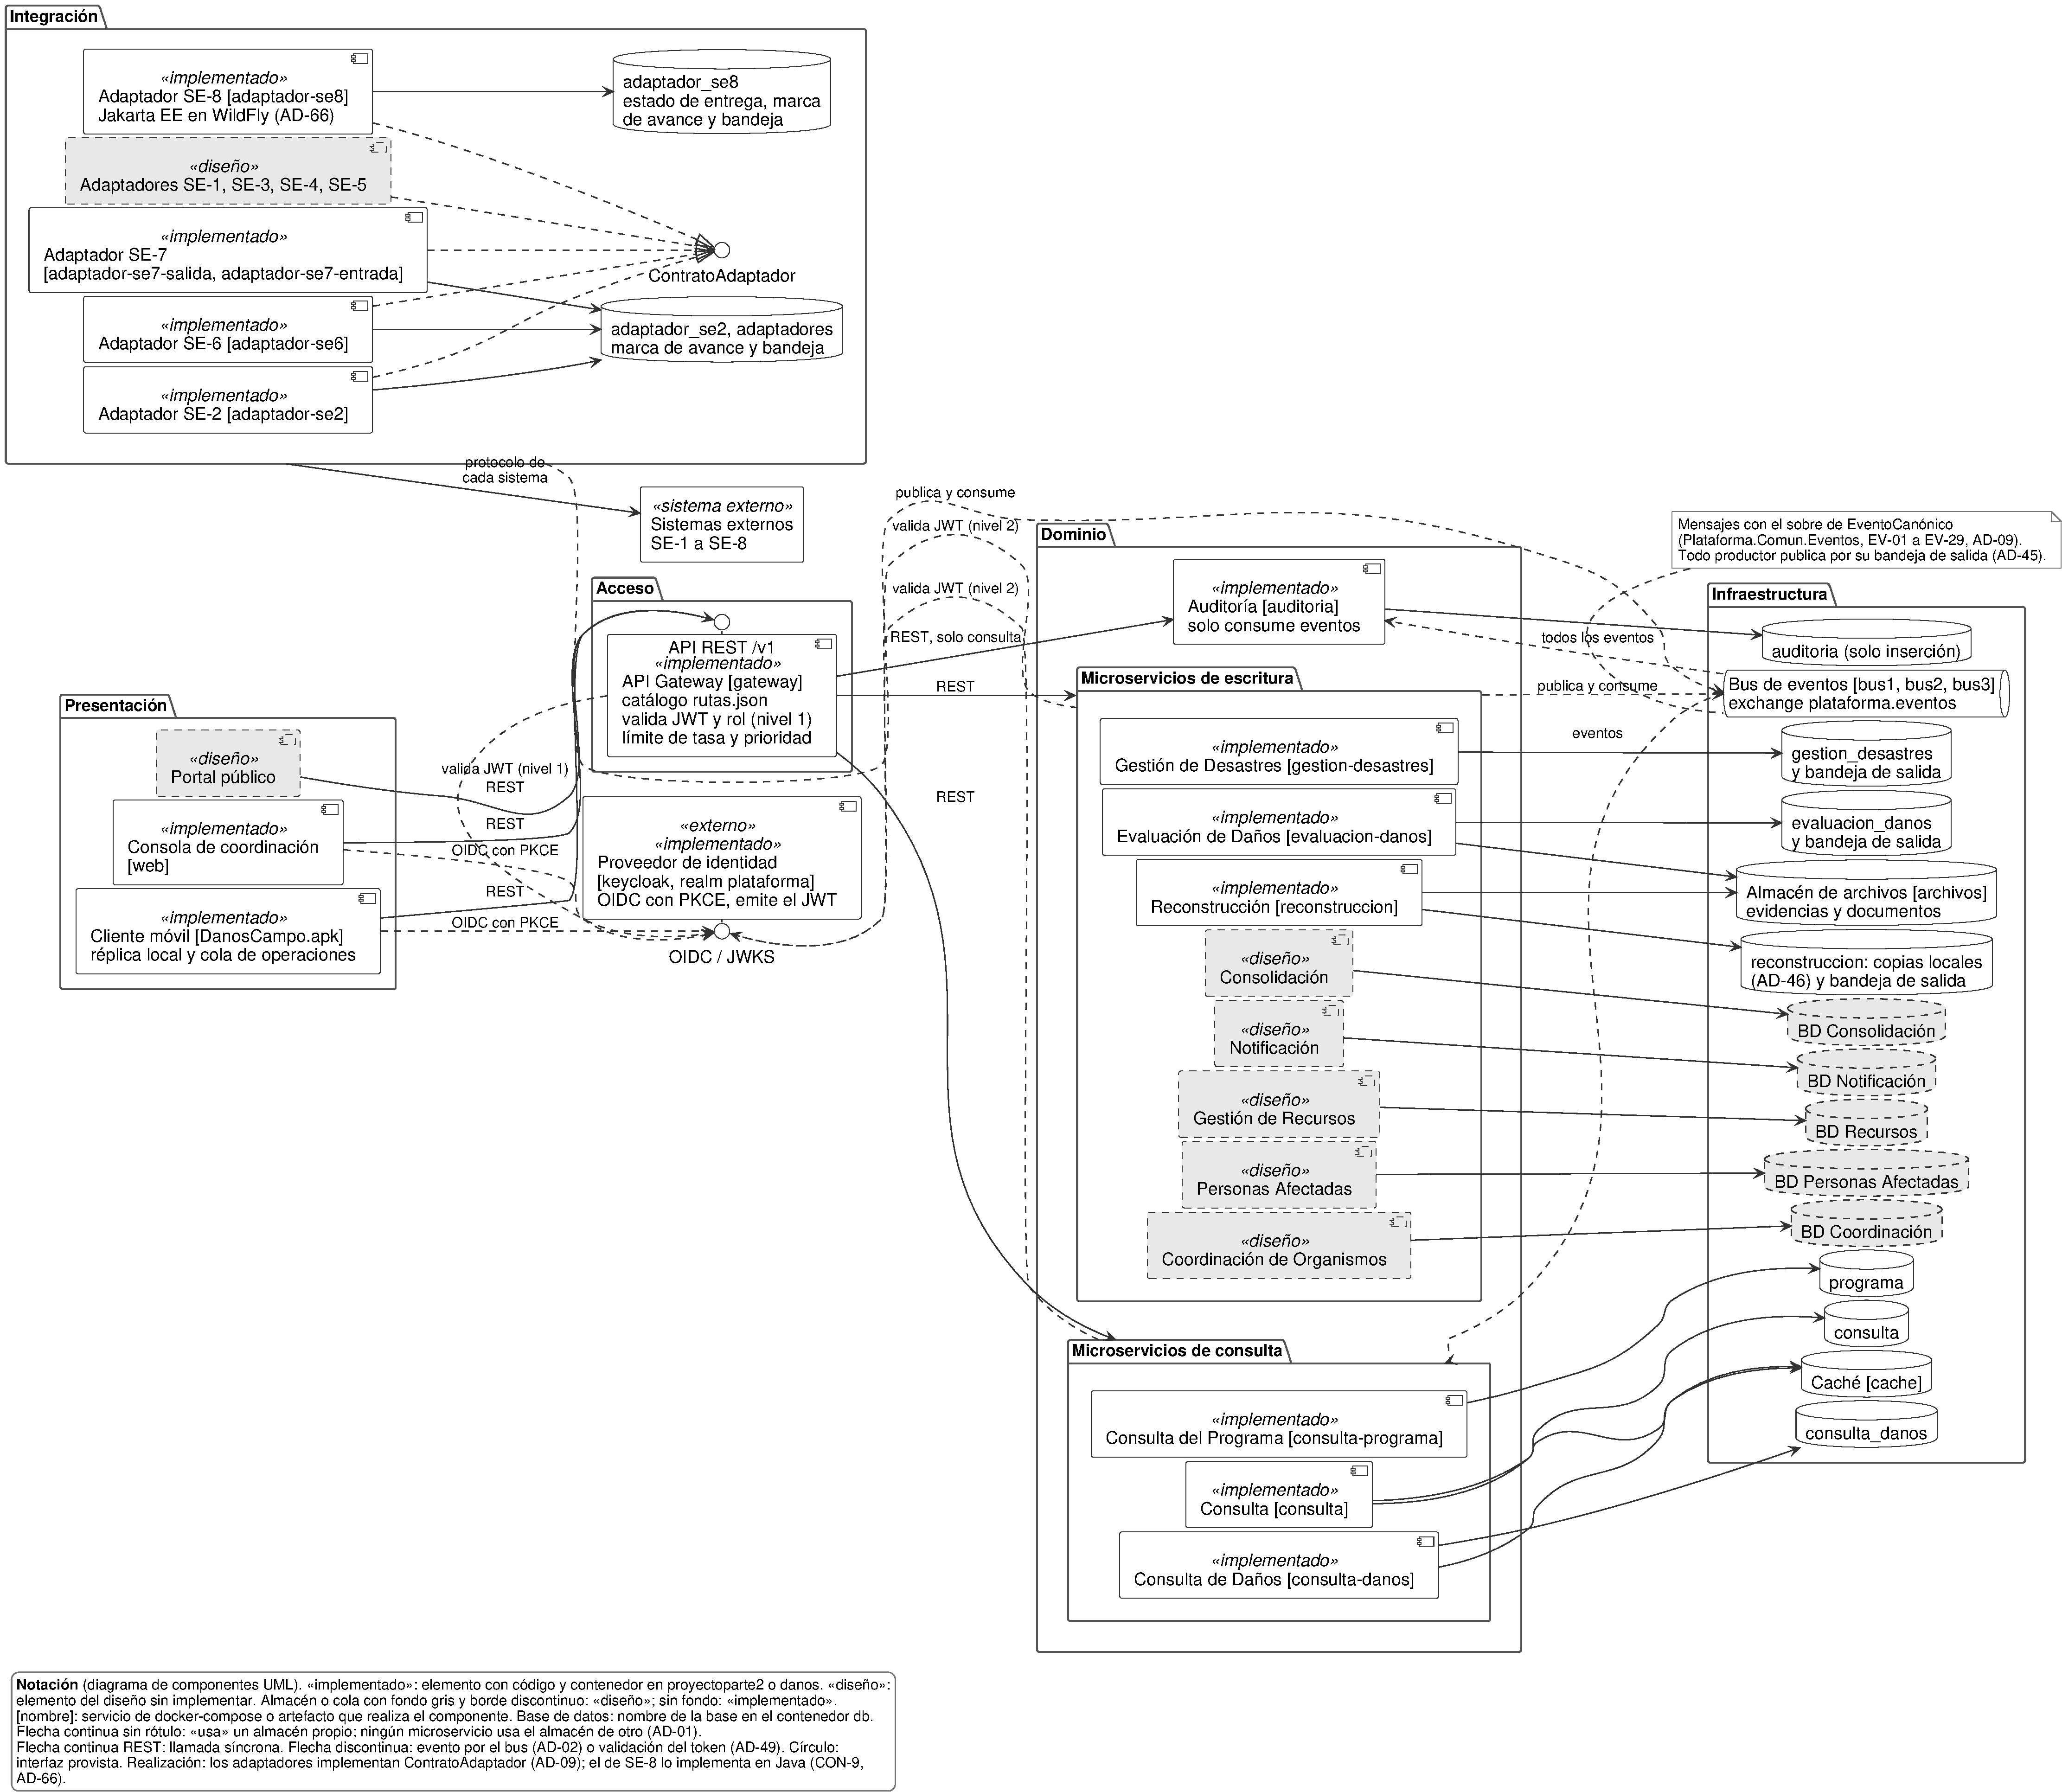
\includegraphics[width=\linewidth,height=0.95\textheight,keepaspectratio]{figuras/vista_logica}
\caption{Vista lógica. Diagrama de componentes UML por capas.}
\label{fig:vista-logica}
\end{figure}
\end{landscape}

El \cref{tab:responsabilidades} indica la responsabilidad de cada elemento de la vista lógica.

\begin{longtable}{L{2.6cm} L{4.0cm} L{9.2cm}}
\cabecera{3}{tab:responsabilidades}{Responsabilidad de los elementos de la vista
lógica}{\textbf{Capa} & \textbf{Elemento} & \textbf{Responsabilidad}}
Presentación & Consola de coordinación & Interfaz de los organismos de respuesta, las autoridades,
el operador, el administrador y el auditor. Tiene prioridad sobre el portal público (AD-19). \\
Presentación & Portal público & Interfaz del ciudadano: consulta de información pública y registro
de solicitudes de ayuda. \\
Presentación & Cliente móvil & Interfaz del evaluador de campo. Opera sobre una réplica local y
sincroniza por lotes (AD-31, AD-44). \\
Presentación & Tablero de daños & Páginas Razor de \texttt{ConsultaDanos.\br{}Api}
(\texttt{/\br{}tablero-\br{}danos}) con el consolidado, la priorización y los indicadores de revisión. Son
un segundo adaptador de entrada de Consulta de Daños: llaman en el mismo proceso a
\texttt{ConsultarConsolidado} y \texttt{ConsultarIndicadores}, los casos de uso de su API. Dominio y
Aplicación no cambian (AD-08, E-41). \\
Acceso & API Gateway & Autentica, valida el rol y la organización (primer nivel de AD-22), limita
la tasa por cliente y prioriza (AD-04, AD-19). \\
Externo & Proveedor de identidad & Autentica a los usuarios con OpenID Connect y PKCE, administra
roles y organizaciones y firma los tokens que validan el API Gateway y los microservicios
(AD-49). \\
Dominio & Gestión de Desastres & Registra y actualiza los desastres, también desde el cliente móvil
con identificador del cliente (AD-48). Administra el catálogo de tipos, los perfiles de ciclo de
vida y los niveles (AD-06, AD-07). Conserva el historial versionado de severidad y delimitación
(AD-20). Impide cerrar un desastre con proyectos no finales (AD-47). \\
Dominio & Consolidación & Correlaciona los reportes de distintas fuentes y conserva la procedencia
de cada dato (AD-10, AD-11, AD-12). \\
Dominio & Notificación & Resuelve las suscripciones y conserva el estado de entrega de cada
notificación (AD-13). \\
Dominio & Evaluación de Daños & Registra las evaluaciones, administra el catálogo de tipos de
activo, recibe la sincronización del cliente móvil y detecta conflictos y duplicados (AD-28 a
AD-33, AD-43, AD-45). \\
Dominio & Gestión de Recursos & Mantiene el catálogo consolidado de recursos con su origen y
gestiona la reserva con plazo de expiración (AD-35, AD-38, AD-39). \\
Dominio & Reconstrucción & Crea proyectos por lote y conserva el historial de solo inserción de
presupuesto y estado (AD-40, AD-41). Obtiene las candidatas de su copia local de desastres,
evaluaciones validadas y municipios (AD-46). \\
Dominio & Personas Afectadas & Registra personas, familias, necesidades y refugios. Cifra los campos
identificatorios (AD-23). \\
Dominio & Coordinación de Organismos & Registra responsabilidades, tareas, prioridades y avances
entre organismos. Aplica la regla del organismo responsable (AD-22). \\
Dominio & Consulta, Consulta de Daños y Consulta del Programa & Atienden las lecturas de mayor
carga a partir de proyecciones alimentadas por eventos (AD-15, AD-34, AD-42). \\
Dominio & Auditoría & Persiste en un registro inmutable los eventos de cambio de todos los
microservicios (AD-21). \\
Infraestructura & Almacenes de escritura & Un almacén por microservicio de escritura. Ocho en
total. \\
Infraestructura & Proyecciones y caché de geometrías & Almacenes de los microservicios de consulta.
La caché guarda la geometría calculada de cada zona (AD-17). \\
Infraestructura & Registro de auditoría & Almacén de solo inserción del microservicio de
Auditoría. \\
Infraestructura & Bus de eventos & Transporta los eventos por el exchange
\texttt{plataforma.\br{}eventos}, con una cola acotada por consumidor y su cola de mensajes muertos
(AD-02, \cref{tab:colas}). \\
Infraestructura (paquete Integración) & \texttt{ContratoAdaptador} y \texttt{EventoCanónico} & Interfaz que implementan
los adaptadores y esquema de datos de los mensajes (AD-09). \\
Infraestructura (paquete Integración) & Adaptadores & Uno por sistema externo. Traducen entre el
formato externo y el evento canónico. Cada uno tiene cortacircuitos, cola de salida y marca de avance
(AD-03, AD-05, AD-14, AD-36). El de SE-8 está en Java sobre Jakarta EE (AD-66) y los demás en .NET \\
\end{longtable}

AD-08 define cuatro capas. El paquete Integración de la \cref{fig:vista-logica} no es una quinta capa:
agrupa los elementos de la capa de infraestructura que conectan con los sistemas externos, es decir,
los adaptadores, \texttt{ContratoAdaptador} y la base con su marca de avance. Se dibuja aparte para
mostrar esa frontera.

\subsection{Vista de procesos}
\label{sec:vista-procesos}

La \cref{fig:vista-procesos} muestra los elementos en ejecución. Cada proceso lleva el estereotipo
\enquote{process} y el número de réplicas entre corchetes. Las flechas continuas son comunicación
síncrona y las discontinuas son comunicación asíncrona por el bus, que es la distinción que exige
CON-5. El bus tiene una cola por consumidor. El diagrama materializa las decisiones siguientes:

\begin{itemize}
  \item AD-24. Los procesos de escritura, el API Gateway y Auditoría tienen al menos dos réplicas
        activas, con sondeo de salud.
  \item AD-18. Los procesos de consulta tienen entre 2 y N réplicas, y N crece con la carga. Los
        procesos de escritura no crecen con la carga de consulta (QA-05).
  \item AD-25. Los adaptadores son procesos efímeros, que se crean cuando llega un evento. El
        proceso \texttt{adaptador-se8} ×1 está siempre encendido para cumplir QA-08: una réplica fija
        en compose y KEDA con mínimo 1 en Kubernetes. Es un proceso de WildFly con cuatro hilos:
        el consumidor JMS, el relevo de la bandeja (\texttt{@Schedule}), el reenvío por falta de
        acuse y el que atiende el aviso de acuse por HTTP.
  \item AD-02. Cada consumidor tiene una cola acotada. El fallo de un consumidor no detiene al
        productor (QA-04). Las colas llevan los nombres de la topología declarada en
        \texttt{despliegue/\br{}bus/\br{}definiciones.\br{}json}: \texttt{q.\br{}reconstruccion},
        \texttt{q.\br{}consulta-\br{}programa}, \texttt{q.\br{}consulta-\br{}danos}, \texttt{q.consulta},
        \texttt{q.\br{}gestion-\br{}desastres}, \texttt{q.\br{}evaluacion-\br{}danos}, \texttt{q.auditoria},
        \texttt{q.salida.se6}, \texttt{q.salida.se7}, \texttt{q.\br{}notificacion} y
        \texttt{q.salida.se8}, cada una con su cola \texttt{dlq.*} (\cref{tab:colas}).
  \item AD-45. Todo proceso productor (\texttt{gestion-\br{}desastres}, \texttt{evaluacion-\br{}danos},
        \texttt{reconstruccion} y los adaptadores) escribe sus eventos en su bandeja de salida y
        tiene un relevo que los publica en el bus. Ningún productor publica fuera de la transacción
        que modifica sus datos (E-19).
  \item AD-46 y AD-47. \texttt{reconstruccion} consume \texttt{q.\br{}reconstruccion} para mantener sus
        copias locales. \texttt{gestion-\br{}desastres} consume \texttt{q.\br{}gestion-\br{}desastres} para contar
        los proyectos no finales de cada desastre.
  \item AD-42. \texttt{consulta-\br{}programa} es el mismo artefacto que \texttt{reconstruccion},
        ejecutado como otro proceso con el rol de consulta.
\end{itemize}

\begin{landscape}
\begin{figure}[p]
\centering
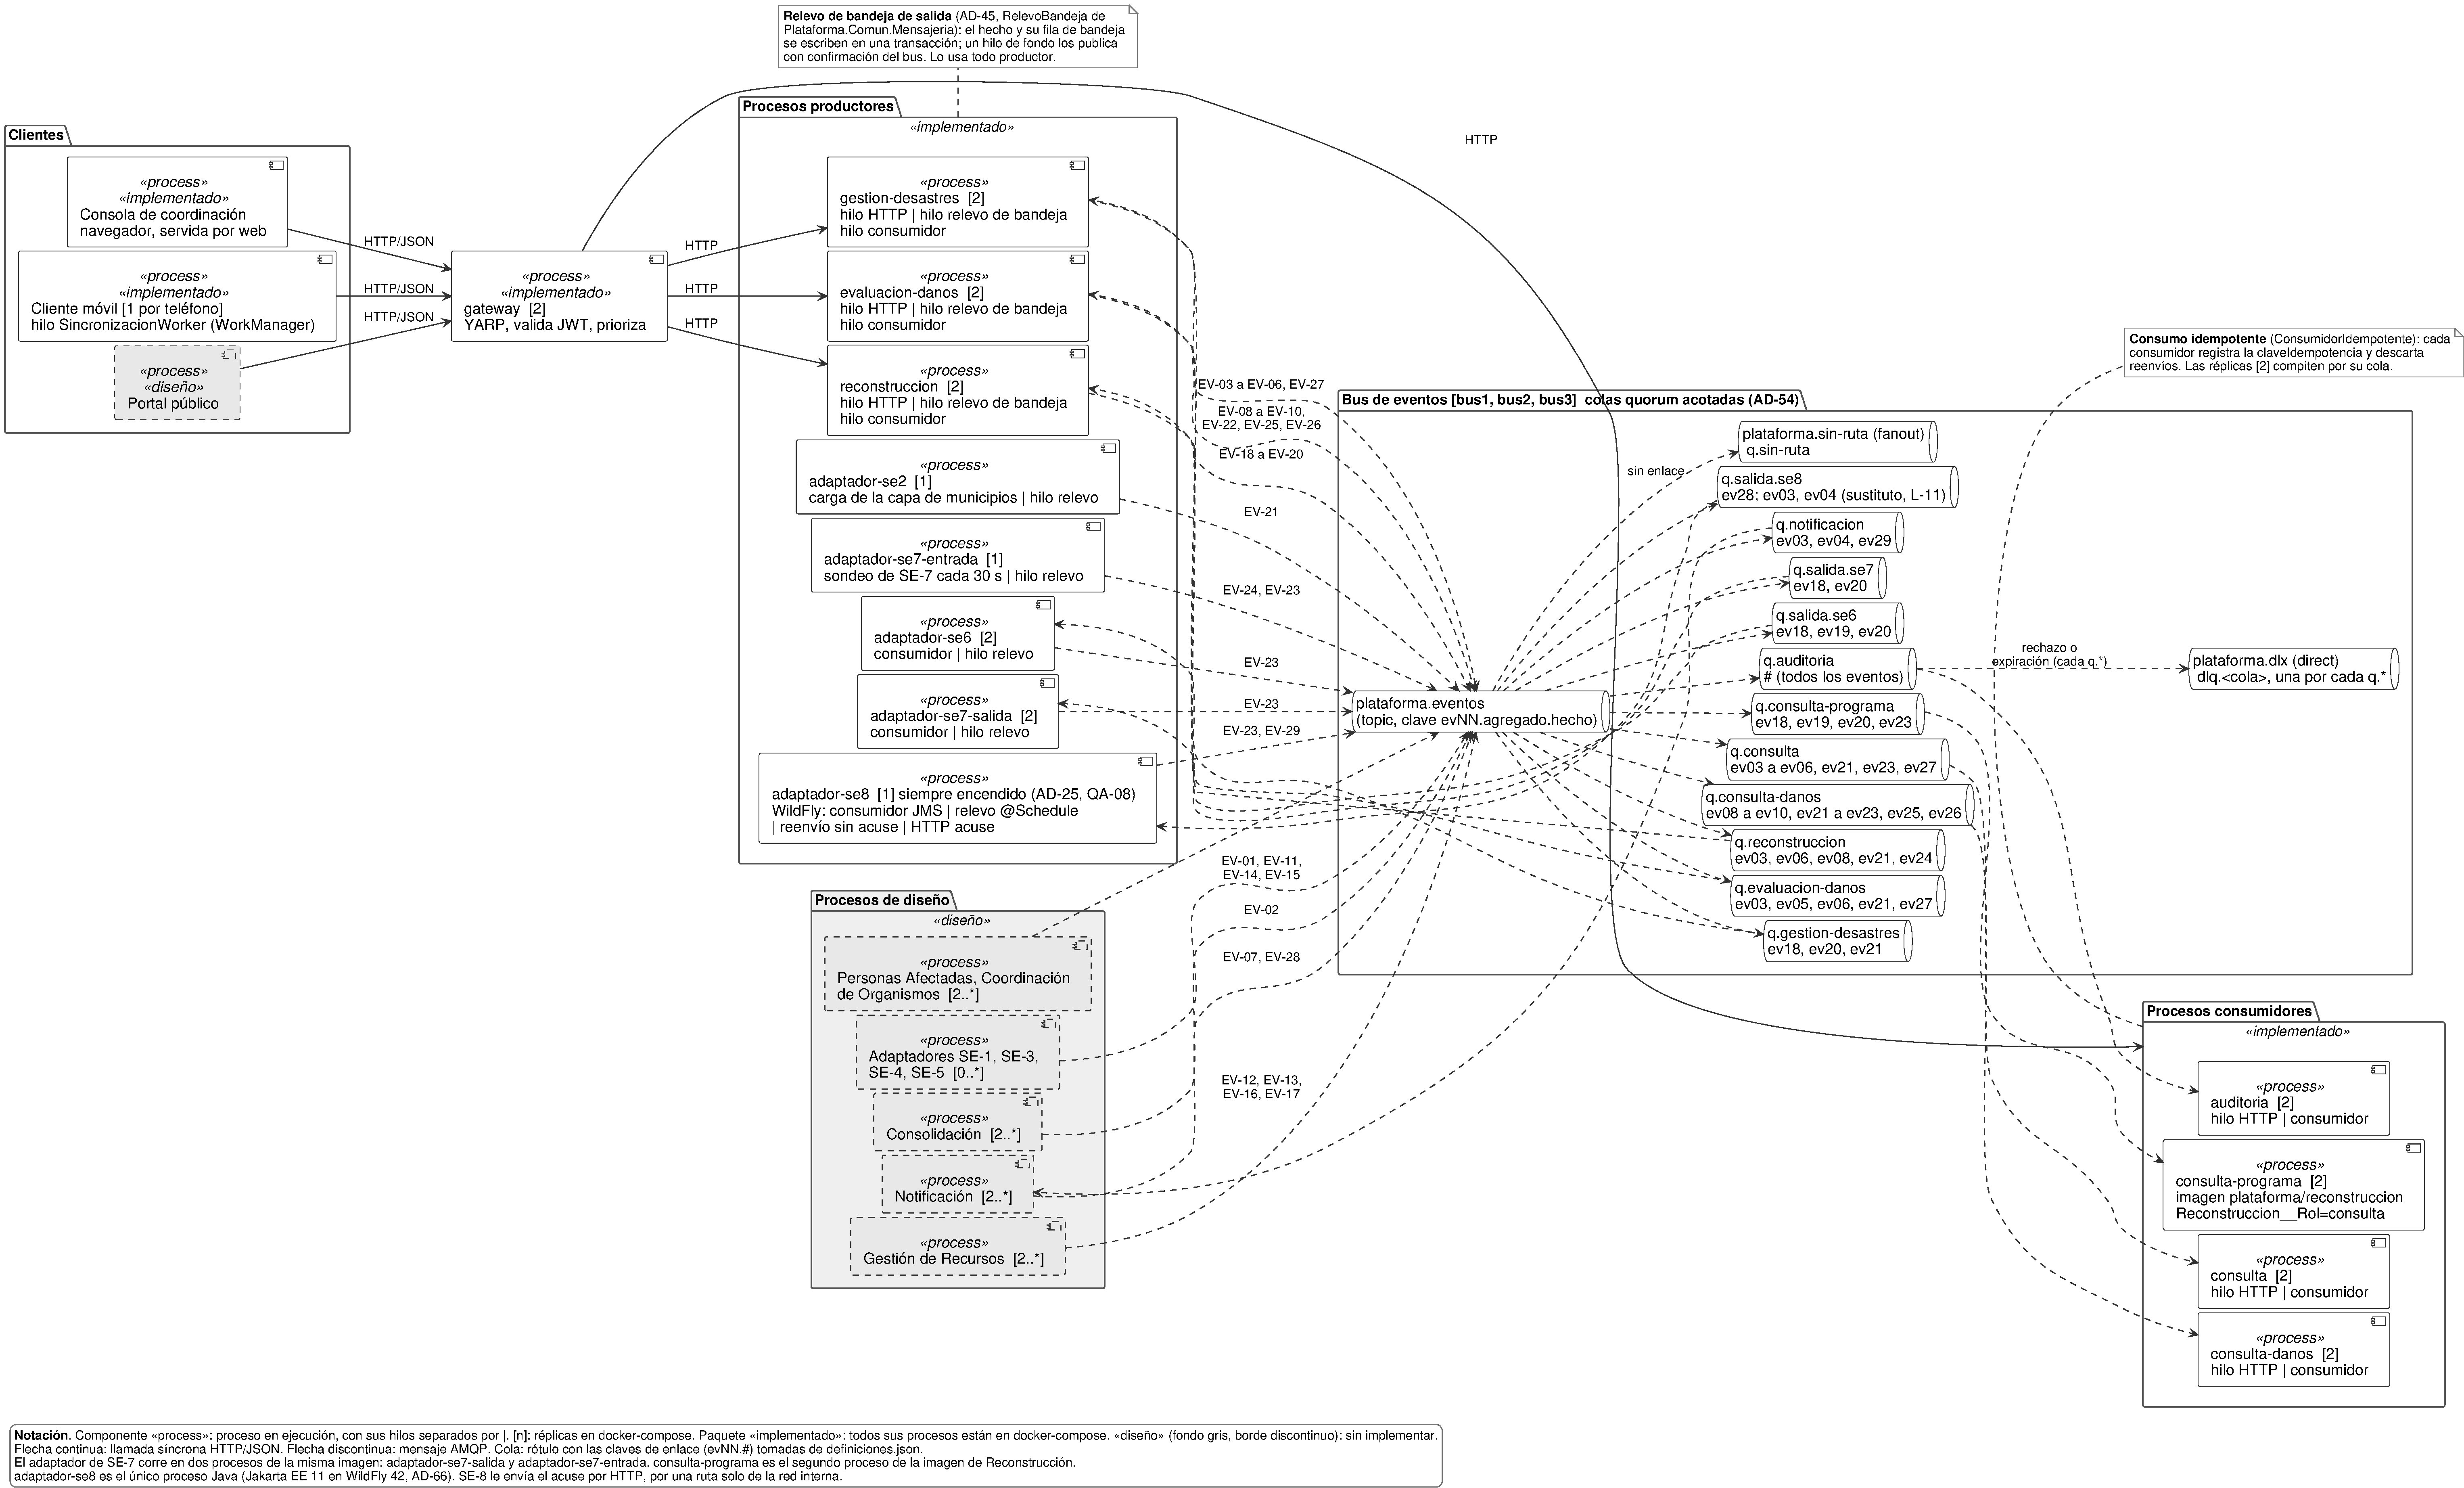
\includegraphics[width=\linewidth,height=0.95\textheight,keepaspectratio]{figuras/vista_procesos}
\caption{Vista de procesos. Procesos en ejecución, réplicas, colas por consumidor y tácticas de
resiliencia.}
\label{fig:vista-procesos}
\end{figure}
\end{landscape}

El \cref{tab:tacticas-procesos} indica en qué proceso actúa cada táctica de resiliencia y a qué rama
del árbol de tácticas de Bass, Clements y Kazman pertenece \cite{bass}.

\begin{longtable}{L{2.5cm} L{2.8cm} L{5.0cm} L{1.6cm} L{3.4cm}}
\cabecera{5}{tab:tacticas-procesos}{Tácticas de resiliencia y proceso en el que actúan}{\textbf{Táctica}
& \textbf{Dónde actúa} & \textbf{Comportamiento} & \textbf{Decisión} & \textbf{Rama de Bass}}
Cortacircuitos & En cada adaptador, sobre las llamadas a su sistema externo & Se abre cuando, con al
menos tres llamadas en \qty{30}{\second}, el \qty{100}{\percent} falla, y permanece abierto \qty{15}{\second} antes de una
llamada de prueba. Mientras está abierto, el adaptador no invoca al sistema externo y publica
EV-23 & AD-05, AD-37, AD-64 & Disponibilidad, prevenir fallos: retirar de servicio \\
Tiempo de espera y reintento & En cada adaptador y en las llamadas del API Gateway a los
microservicios & En los adaptadores implementados: tiempo de espera de \qty{3}{\second} por intento
y \qty{20}{\second} por operación, y dos reintentos con espera exponencial desde
\qty{0,5}{\second}. Solo se reintentan operaciones idempotentes. El adaptador de SE-8 aplica los
mismos valores con su ejecutor propio (AD-66) & AD-05, AD-64, AD-66 & Disponibilidad, detectar fallos (tiempo de espera) y recuperarse de fallos (reintento) \\
Cola acotada & En cada cola \texttt{q.*} del bus & Límite de \num{100000} mensajes y
\qty{256}{\mega\byte}. Al llenarse, la cola rechaza la publicación y el evento permanece en la bandeja del
productor. Ningún evento se descarta (E-23) & AD-02, AD-54 & Rendimiento, gestionar recursos: acotar las colas \\
Cola de salida & En el bus, una por adaptador & Acumula los mensajes dirigidos a un sistema
externo no disponible y los entrega cuando el circuito se cierra & AD-36 & Disponibilidad, recuperarse de fallos: reintento diferido \\
Marca de avance & En cada adaptador & Al cerrarse el circuito, el adaptador pide el rango pendiente
desde el último dato recibido & AD-14, AD-37 & Disponibilidad, recuperarse de fallos: resincronización de estado \\
Reenvío por falta de acuse & En el adaptador de SE-8 & Es distinto del reintento de la llamada: SE-8
sí recibió la alerta, pero no la acusó. Una alerta sin acuse en \qty{5}{\second} vuelve a pendiente
y se reenvía con la misma referencia. Al quinto envío queda fallida. Con EV-28, el reintento lo
decide Notificación (AD-13) & AD-13, AD-66 & Disponibilidad, recuperarse de fallos: reintento \\
Degradación controlada & En el API Gateway y en los microservicios de consulta & El API Gateway
reduce primero el portal público. La consulta devuelve el último dato conocido con su marca de
tiempo & AD-16, AD-19 & Disponibilidad, recuperarse de fallos: degradación \\
Réplica activa con sondeo de salud & En los procesos persistentes & Una réplica que no responde al
sondeo deja de recibir tráfico en \qty{30}{\second} o menos & AD-24 & Disponibilidad, detectar fallos (sondeo) y recuperarse de fallos (repuesto redundante) \\
Consumo idempotente & En cada consumidor del bus & Un mensaje entregado más de una vez se procesa
una sola vez, por la clave de idempotencia. Un fallo transitorio se reintenta hasta cinco entregas.
Al superarlas, o si el mensaje no cumple el contrato, el consumidor lo aparta a su cola
\texttt{dlq.*} (E-32) & AD-02, AD-14 & Disponibilidad, recuperarse de fallos: reintento seguro y manejo de excepciones \\
Bandeja de salida & En cada microservicio productor & El relevo publica los eventos que la
transacción dejó en la bandeja y les asigna la secuencia del productor. Si el bus no está
disponible, el evento permanece en la bandeja (E-19, E-31) & AD-45 & Disponibilidad, prevenir fallos: transacciones \\
\end{longtable}

\subsection{Vista física}
\label{sec:vista-fisica}

La \cref{fig:vista-despliegue} es un diagrama de despliegue UML. Los nodos con estereotipo
\enquote{device} contienen nodos \enquote{executionEnvironment}, y en estos se despliegan los
artefactos. Las rutas de comunicación indican el mecanismo. La vista física se presenta en dos
diagramas. La \cref{fig:vista-despliegue} muestra el despliegue de diseño en dos regiones, con los
nodos descritos por su función. La \cref{fig:vista-despliegue-impl} muestra el despliegue de la
implementación, con los artefactos reales y las tecnologías de la \cref{sec:tecnologia}. En el
diagrama de diseño, los artefactos implementados usan el nombre del servicio del compose, y los
de diseño usan un nombre propuesto con la misma convención (\texttt{consolidacion},
\texttt{notificacion}, \texttt{gestion-recursos}, \texttt{personas-afectadas} y
\texttt{coordinacion-organismos}). El diagrama de diseño materializa las decisiones siguientes:

\begin{itemize}
  \item AD-26. Hay dos regiones geográficas. La región primaria atiende todo el tráfico. La región
        secundaria tiene los microservicios desplegados con capacidad mínima y recibe los datos por
        replicación asíncrona, lo que fija un RPO $\le$ \qty{60}{\second} (QA-03). El enrutador
        global sondea la región primaria y conmuta el tráfico si deja de responder.
  \item AD-27. Cuando la región primaria se recupera, sus almacenes se resincronizan antes de
        recibir tráfico.
  \item AD-24 y AD-18. La multiplicidad de cada artefacto indica sus réplicas: al menos dos para los
        microservicios persistentes y entre 2 y N para los de consulta.
  \item AD-25. Los adaptadores se despliegan en un entorno de ejecución efímera, separado del
        entorno de los microservicios persistentes.
  \item AD-31. El dispositivo móvil del evaluador contiene el artefacto del cliente móvil y su
        réplica local, que es una base de datos embebida.
  \item AD-49. El Proveedor de identidad se despliega en su propio nodo. Los clientes lo invocan
        para obtener el token, y el API Gateway y los microservicios lo consultan para obtener las
        llaves con que validan la firma.
\end{itemize}

\begin{landscape}
\begin{figure}[p]
\centering
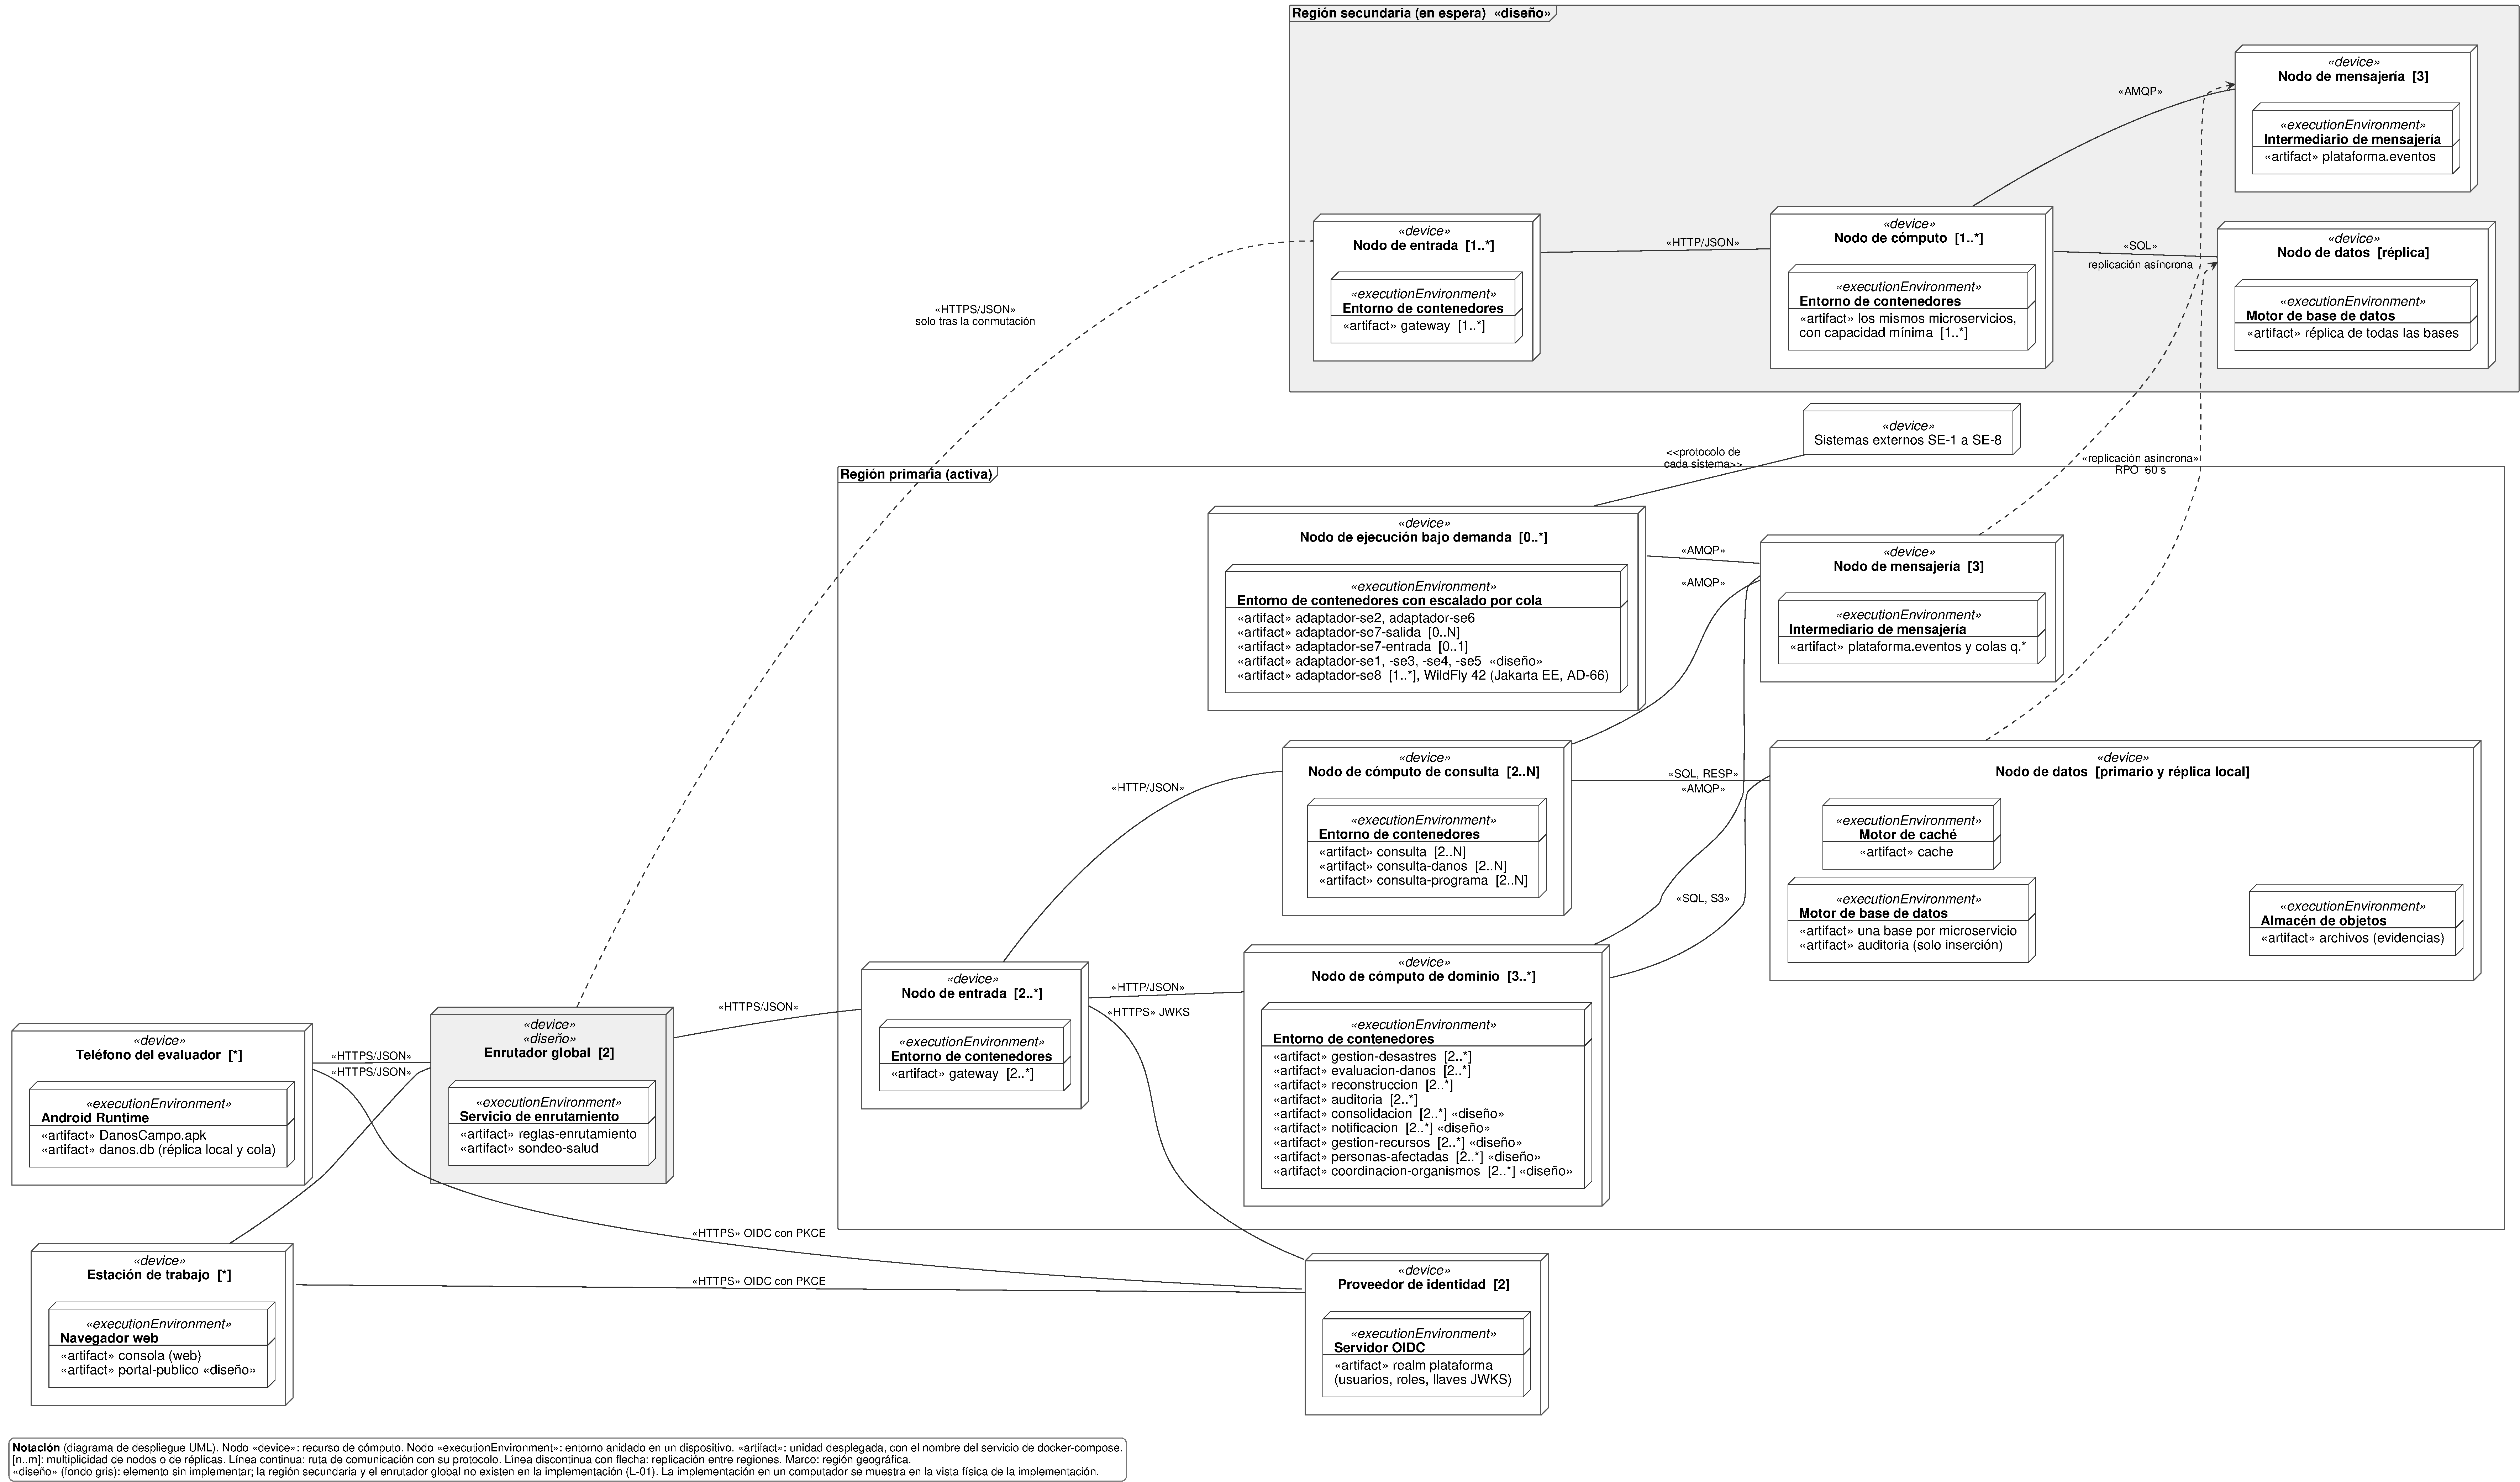
\includegraphics[width=\linewidth,height=0.95\textheight,keepaspectratio]{figuras/vista_despliegue}
\caption{Vista física. Diagrama de despliegue UML con dos regiones.}
\label{fig:vista-despliegue}
\end{figure}
\end{landscape}

\begin{longtable}{L{4.4cm} L{3.4cm} L{8.0cm}}
\cabecera{3}{tab:nodos}{Nodos de la vista física}{\textbf{Nodo} & \textbf{Multiplicidad} &
\textbf{Función}}
Dispositivo móvil del evaluador & Uno por evaluador & Ejecuta el cliente móvil y almacena la réplica
local y la cola de operaciones (AD-31, AD-44). \\
Estación de trabajo & Una por usuario & Ejecuta la consola de coordinación o el portal público en
un navegador. \\
Enrutador global & 2 & Dirige el tráfico a la región activa y conmuta a la secundaria (AD-26). \\
Nodo de entrada & 2 o más en la primaria; 1 o más en la secundaria & Ejecuta el API Gateway
(AD-04). \\
Nodo de cómputo de dominio & 3 o más & Ejecuta los ocho microservicios de escritura y el de
Auditoría, con al menos dos réplicas de cada uno (AD-24). \\
Nodo de cómputo de consulta & De 2 a N & Ejecuta los tres microservicios de consulta. Su número
crece con la carga (AD-18). \\
Nodo de ejecución bajo demanda & De 0 en adelante & Ejecuta los adaptadores como unidades efímeras
(AD-25). \\
Nodo de identidad & 2 o más en la primaria; 1 en la secundaria & Ejecuta el Proveedor de
identidad (AD-49). \\
Nodo de mensajería & 3 por región & Ejecuta el bus de eventos (AD-02). \\
Nodo de datos & Primario y réplica local por almacén; réplica en la región secundaria & Aloja los
almacenes de escritura, las proyecciones, el registro de auditoría, la caché de geometrías y las
evidencias. \\
\end{longtable}

\subsection{Vista física de la implementación}
\label{sec:vista-fisica-impl}

La \cref{fig:vista-despliegue-impl} es el diagrama de despliegue UML de la entrega 2. Corresponde
uno a uno con el archivo \texttt{despliegue/\br{}compose/\br{}docker-\br{}compose.\br{}yml} y con el cliente móvil del
repositorio \texttt{danos} (regla del diagrama que corresponde al código). Tiene dos nodos
\enquote{device}:

\begin{itemize}
  \item El computador (Windows 11), con dos entornos de ejecución. En Docker Engine con Docker
        Compose se despliega un contenedor por servicio del compose, con su nombre exacto y su
        multiplicidad, agrupados en entrada e identidad, microservicios, adaptadores y simuladores,
        datos y mensajería, y migradores (AD-24, AD-65). Dentro del contenedor
        \texttt{adaptador-se8} hay un entorno de ejecución más: el servidor Jakarta EE WildFly
        42.0.0.Final sobre Java 21, con el artefacto \texttt{adaptador-se8.war} (AD-66). En el
        navegador se ejecuta la Consola de coordinación servida por \texttt{web} (AD-59).
  \item El teléfono Android del evaluador, con el entorno de ejecución de Android. En él se
        despliegan \texttt{DanosCampo.\br{}apk} y la base \texttt{danos.db} (AD-31, AD-61, AD-62).
\end{itemize}

Las rutas de comunicación indican el protocolo y el puerto. Los clientes llegan solo al
\texttt{gateway} por HTTP con el token \emph{Bearer} (puerto 8080) y a \texttt{keycloak} por
OpenID Connect con PKCE (puerto 8180) (AD-04, AD-49). Los microservicios publican y consumen por
AMQP en \texttt{bus1}, \texttt{bus2} y \texttt{bus3} y usan SQL contra \texttt{db}, que replica por
\emph{streaming} a \texttt{db-replica} (AD-52, AD-54). Una nota indica el despliegue equivalente en
Kubernetes (\texttt{despliegue/\br{}k8s}). En esos manifiestos, un HPA escala \texttt{consulta},
\texttt{consulta-\br{}danos} y \texttt{consulta-\br{}programa}, y KEDA escala por longitud de cola
\texttt{adaptador-se6} y \texttt{adaptador-se7-salida}, enciende \texttt{adaptador-se7-entrada} con
un disparador de horario y mantiene \texttt{adaptador-se8} entre 1 y 2 réplicas (AD-18, AD-25, AD-65).
El simulador \texttt{sim-se8} avisa el acuse por \texttt{POST /v1/acuses}, una ruta solo de la red
interna del compose: el \texttt{gateway} no la enruta. Esta vista no tiene segunda región (L-01). El \cref{tab:nodos-impl} lista los
artefactos.

\begin{landscape}
\begin{figure}[p]
\centering
\includegraphics[width=\linewidth,height=0.95\textheight,keepaspectratio]{figuras/vista_despliegue_implementacion}
\caption{Vista física de la implementación. Diagrama de despliegue UML del compose y del teléfono
Android.}
\label{fig:vista-despliegue-impl}
\end{figure}
\end{landscape}

\begingroup\small
\begin{longtable}{L{3.4cm} L{4.4cm} L{1.5cm} L{6.2cm}}
\cabecera{4}{tab:nodos-impl}{Nodos y artefactos de la vista física de la implementación}{\textbf{Artefacto}
& \textbf{Imagen o archivo} & \textbf{Réplicas} & \textbf{Elemento del diseño y decisión}}
\multicolumn{4}{@{}l}{\textit{Device: computador. Entorno de ejecución: Docker Engine con Docker Compose}} \\
\texttt{gateway} & \texttt{plataforma/\br{}gateway:\br{}local} con \texttt{rutas.json} & 2 & API Gateway.
Puertos 8080 y 8081 (AD-04, AD-19, AD-57) \\
\texttt{keycloak} & \texttt{quay.\br{}io/\br{}keycloak/\br{}keycloak:\br{}26.\br{}5.\br{}2}, realm \texttt{plataforma} & 1 &
Proveedor de identidad. Puerto 8180 (AD-49, AD-58) \\
\texttt{web} & Consola Angular servida por nginx & 1 & Consola de coordinación (AD-59, AD-60) \\
\texttt{gestion-\br{}desastres} & \texttt{plataforma/\br{}gestion-\br{}desastres:\br{}local} & 2 & Gestión de Desastres
(AD-06, AD-47, AD-48) \\
\texttt{evaluacion-\br{}danos} & \texttt{plataforma/\br{}evaluacion-\br{}danos:\br{}local} & 2 & Evaluación de Daños
(AD-28 a AD-33, AD-43 a AD-45) \\
\texttt{reconstruccion} & \texttt{plataforma/\br{}reconstruccion:\br{}local}, rol de escritura & 2 &
Reconstrucción (AD-40, AD-41, AD-46) \\
\texttt{consulta-\br{}programa} & \texttt{plataforma/\br{}reconstruccion:\br{}local} con
\texttt{Reconstruccion\_\br{}\_\br{}Rol=consulta} & 2 & Consulta del Programa (AD-42) \\
\texttt{consulta} & \texttt{plataforma/\br{}consulta:\br{}local} & 2 & Consulta (AD-15, AD-17) \\
\texttt{consulta-\br{}danos} & \texttt{plataforma/\br{}consulta-\br{}danos:\br{}local} & 2 & Consulta de Daños y tablero
\texttt{/\br{}tablero-\br{}danos} (AD-34) \\
\texttt{auditoria} & \texttt{plataforma/\br{}auditoria:\br{}local} & 2 & Auditoría (AD-21) \\
\texttt{adaptador-se2} & \texttt{plataforma/\br{}adaptador-\br{}se2:\br{}local} & 1 & Adaptador de SE-2, produce
EV-21 (AD-03) \\
\texttt{adaptador-se6} & \texttt{plataforma/\br{}adaptador-\br{}se6:\br{}local} & 2 & Adaptador de salida de SE-6
(AD-03, AD-36) \\
\texttt{adaptador-\br{}se7-\br{}salida}, \texttt{adaptador-\br{}se7-\br{}entrada} & \texttt{plataforma/\br{}adaptador-\br{}se7:\br{}local}
& 2 y 1 & Adaptador de SE-7, salida por cola y entrada con marca de avance (AD-14, AD-36) \\
\texttt{sim-se6}, \texttt{sim-se7} & \texttt{plataforma/\br{}sim-\br{}se6:\br{}local},
\texttt{plataforma/\br{}sim-\br{}se7:\br{}local} & 1 & Simuladores de los sistemas externos SE-6 y SE-7 \\
\texttt{adaptador-se8} & \texttt{plataforma/\br{}adaptador-\br{}se8:\br{}local}: entorno de ejecución WildFly
42.0.0.Final (Jakarta EE 11, Java 21) con \texttt{adaptador-se8.war} & 1 & Adaptador de SE-8, siempre
encendido (AD-03, AD-25, AD-66) \\
\texttt{adaptador-\br{}se8-\br{}migrador} & \texttt{plataforma/\br{}adaptador-\br{}se8-\br{}migrador:\br{}local}
(Java 21, Flyway) & 1 & Crea la base \texttt{adaptador\_\br{}se8} y su rol de mínimo privilegio y termina
(AD-53, AD-66) \\
\texttt{sim-se8} & \texttt{plataforma/\br{}sim-\br{}se8:\br{}local} & 1 & Simulador de SE-8: recibe alertas y
avisa el acuse \\
\texttt{*-migrador} & La imagen de cada microservicio & 1 & Aplica las migraciones y termina
(AD-53) \\
\texttt{bus1}, \texttt{bus2}, \texttt{bus3} & \texttt{rabbitmq:\br{}4.\br{}4.\br{}0-\br{}management} con
\texttt{definiciones.\br{}json} & 3 & Bus de eventos (AD-02, AD-54) \\
\texttt{db} & \texttt{postgis/\br{}postgis:\br{}18-\br{}3.\br{}6} & 1 & Almacenes: bases \texttt{gestion\_\br{}desastres},
\texttt{evaluacion\_\br{}danos}, \texttt{reconstruccion}, \texttt{programa}, \texttt{consulta},
\texttt{consulta\_\br{}danos}, \texttt{auditoria}, \texttt{adaptador\_\br{}se2}, \texttt{adaptadores} y
\texttt{adaptador\_\br{}se8} (AD-01, AD-52) \\
\texttt{db-replica} & \texttt{postgis/\br{}postgis:\br{}18-\br{}3.\br{}6} en espera activa & 1 & Réplica de datos
(AD-24, AD-52) \\
\texttt{cache} & \texttt{redis:\br{}8.\br{}8.\br{}4-\br{}alpine} & 1 & Caché de geometrías (AD-17, AD-55) \\
\texttt{archivos} & Almacén de objetos con API S3 & 1 & Almacén de evidencias y documentos
(AD-56) \\
\multicolumn{4}{@{}l}{\textit{Device: teléfono Android. Entorno de ejecución: Android (minSdk 26)}} \\
\texttt{DanosCampo.\br{}apk} & \texttt{co.\br{}plataforma.\br{}danos} 2.1.0 & 1 & Cliente móvil (AD-31, AD-44,
AD-48, AD-61, AD-63) \\
\texttt{danos.db} & Base Room, esquema 3 & 1 & Réplica local y colas de operaciones (AD-31, AD-44,
AD-62) \\
\multicolumn{4}{@{}l}{\textit{Device: computador. Entorno de ejecución: navegador web}} \\
Consola de coordinación & Aplicación Angular descargada de \texttt{web} & 1 & Consola de
coordinación (AD-59) \\
\end{longtable}
\endgroup

\subsection{Vista de implementación}
\label{sec:vista-implementacion}

La vista de implementación se presenta en dos diagramas de paquetes UML con los nombres del
código. La \cref{fig:vista-implementacion} muestra la solución \texttt{Plataforma.\br{}sln} del
repositorio \texttt{proyectoparte2}: los proyectos del microservicio tipo
(\texttt{servicios/evaluacion-danos}, con sus clases principales), los proyectos comunes
\texttt{Plataforma.\br{}Comun.\br{}*}, los adaptadores y el gateway, más el proyecto Maven
\texttt{adaptador-\br{}se8-\br{}jee} con sus paquetes Java. La \cref{fig:vista-implementacion-movil}
muestra los paquetes del módulo \texttt{app} del repositorio \texttt{danos}. Los diagramas
materializan las decisiones siguientes:

\begin{itemize}
  \item AD-08. Cada microservicio se compone de cuatro proyectos .NET: \texttt{*.Api},
        \texttt{*.Aplicacion}, \texttt{*.Dominio} e \texttt{*.\br{}Infraestructura}. Las dependencias
        \enquote{import} van de \texttt{Api} a \texttt{Aplicacion} y de \texttt{Aplicacion} a
        \texttt{Dominio}. \texttt{Infraestructura} implementa los puertos que declara
        \texttt{Aplicacion}, de modo que el dominio no depende de la infraestructura. El
        \cref{tab:equivalencia-capas} relaciona estos proyectos con las cuatro capas del diseño.
  \item AD-01. Ningún proyecto de un microservicio referencia a otro microservicio. Todos dependen
        solo de los proyectos \texttt{Plataforma.\br{}Comun.\br{}*}.
  \item AD-03 y AD-09. Hay un proyecto por adaptador implementado (\texttt{AdaptadorSe2},
        \texttt{AdaptadorSe6} y \texttt{AdaptadorSe7}). Cada uno implementa la interfaz
        \texttt{IContratoAdaptador} de \texttt{Plataforma.\br{}Comun.\br{}Adaptadores} y usa el sobre
        canónico de \texttt{Plataforma.\br{}Comun.\br{}Eventos}. Los adaptadores de SE-1, SE-3, SE-4 y
        SE-5 aparecen con el estereotipo «diseño» (L-06).
  \item AD-66. El adaptador de SE-8 es el paquete Java \texttt{adaptador-\br{}se8-\br{}jee} (Maven, Java
        21, un WAR). Sus clases principales son \texttt{AdaptadorSe8} (EJB \texttt{@Stateless} que
        implementa \texttt{ContratoAdaptador}), \texttt{ManejadorSe8} (unidades de trabajo
        \texttt{REQUIRES\_NEW}), \texttt{ConsumidorSe8} y \texttt{BucleConsumo} (Jakarta Messaging),
        \texttt{Temporizadores} (Timer Service), \texttt{Entrega} (Jakarta Persistence) y
        \texttt{RecursoAcuses} (Jakarta REST). No referencia ningún proyecto .NET: comparte el
        contrato por los esquemas JSON de \texttt{Plataforma.\br{}Comun.\br{}Eventos}, que se copian al
        WAR al compilar.
  \item AD-45. \texttt{Plataforma.\br{}Comun.\br{}Mensajeria} contiene \texttt{EscritorBandeja},
        \texttt{RelevoBandeja} y \texttt{ConsumidorIdempotente}, que usan todos los productores y
        consumidores.
  \item AD-20 y AD-41. El historial versionado y el historial de solo inserción no son un paquete
        común. Cada microservicio los implementa en su proyecto \texttt{*.\br{}Infraestructura}, y su
        migración concede al usuario de la aplicación solo \texttt{SELECT} e \texttt{INSERT} sobre
        las tablas de historial (\texttt{GRANT}). La garantía de inmutabilidad la da la base de
        datos y no el código.
  \item AD-31, AD-44 y AD-48. El cliente móvil contiene la réplica local, las colas de operaciones
        de evaluaciones y de registros de desastre, y la sincronización (\texttt{MotorSincronizacion}
        y \texttt{EnviadorDesastres}).
\end{itemize}

\begin{figure}[p]
\centering
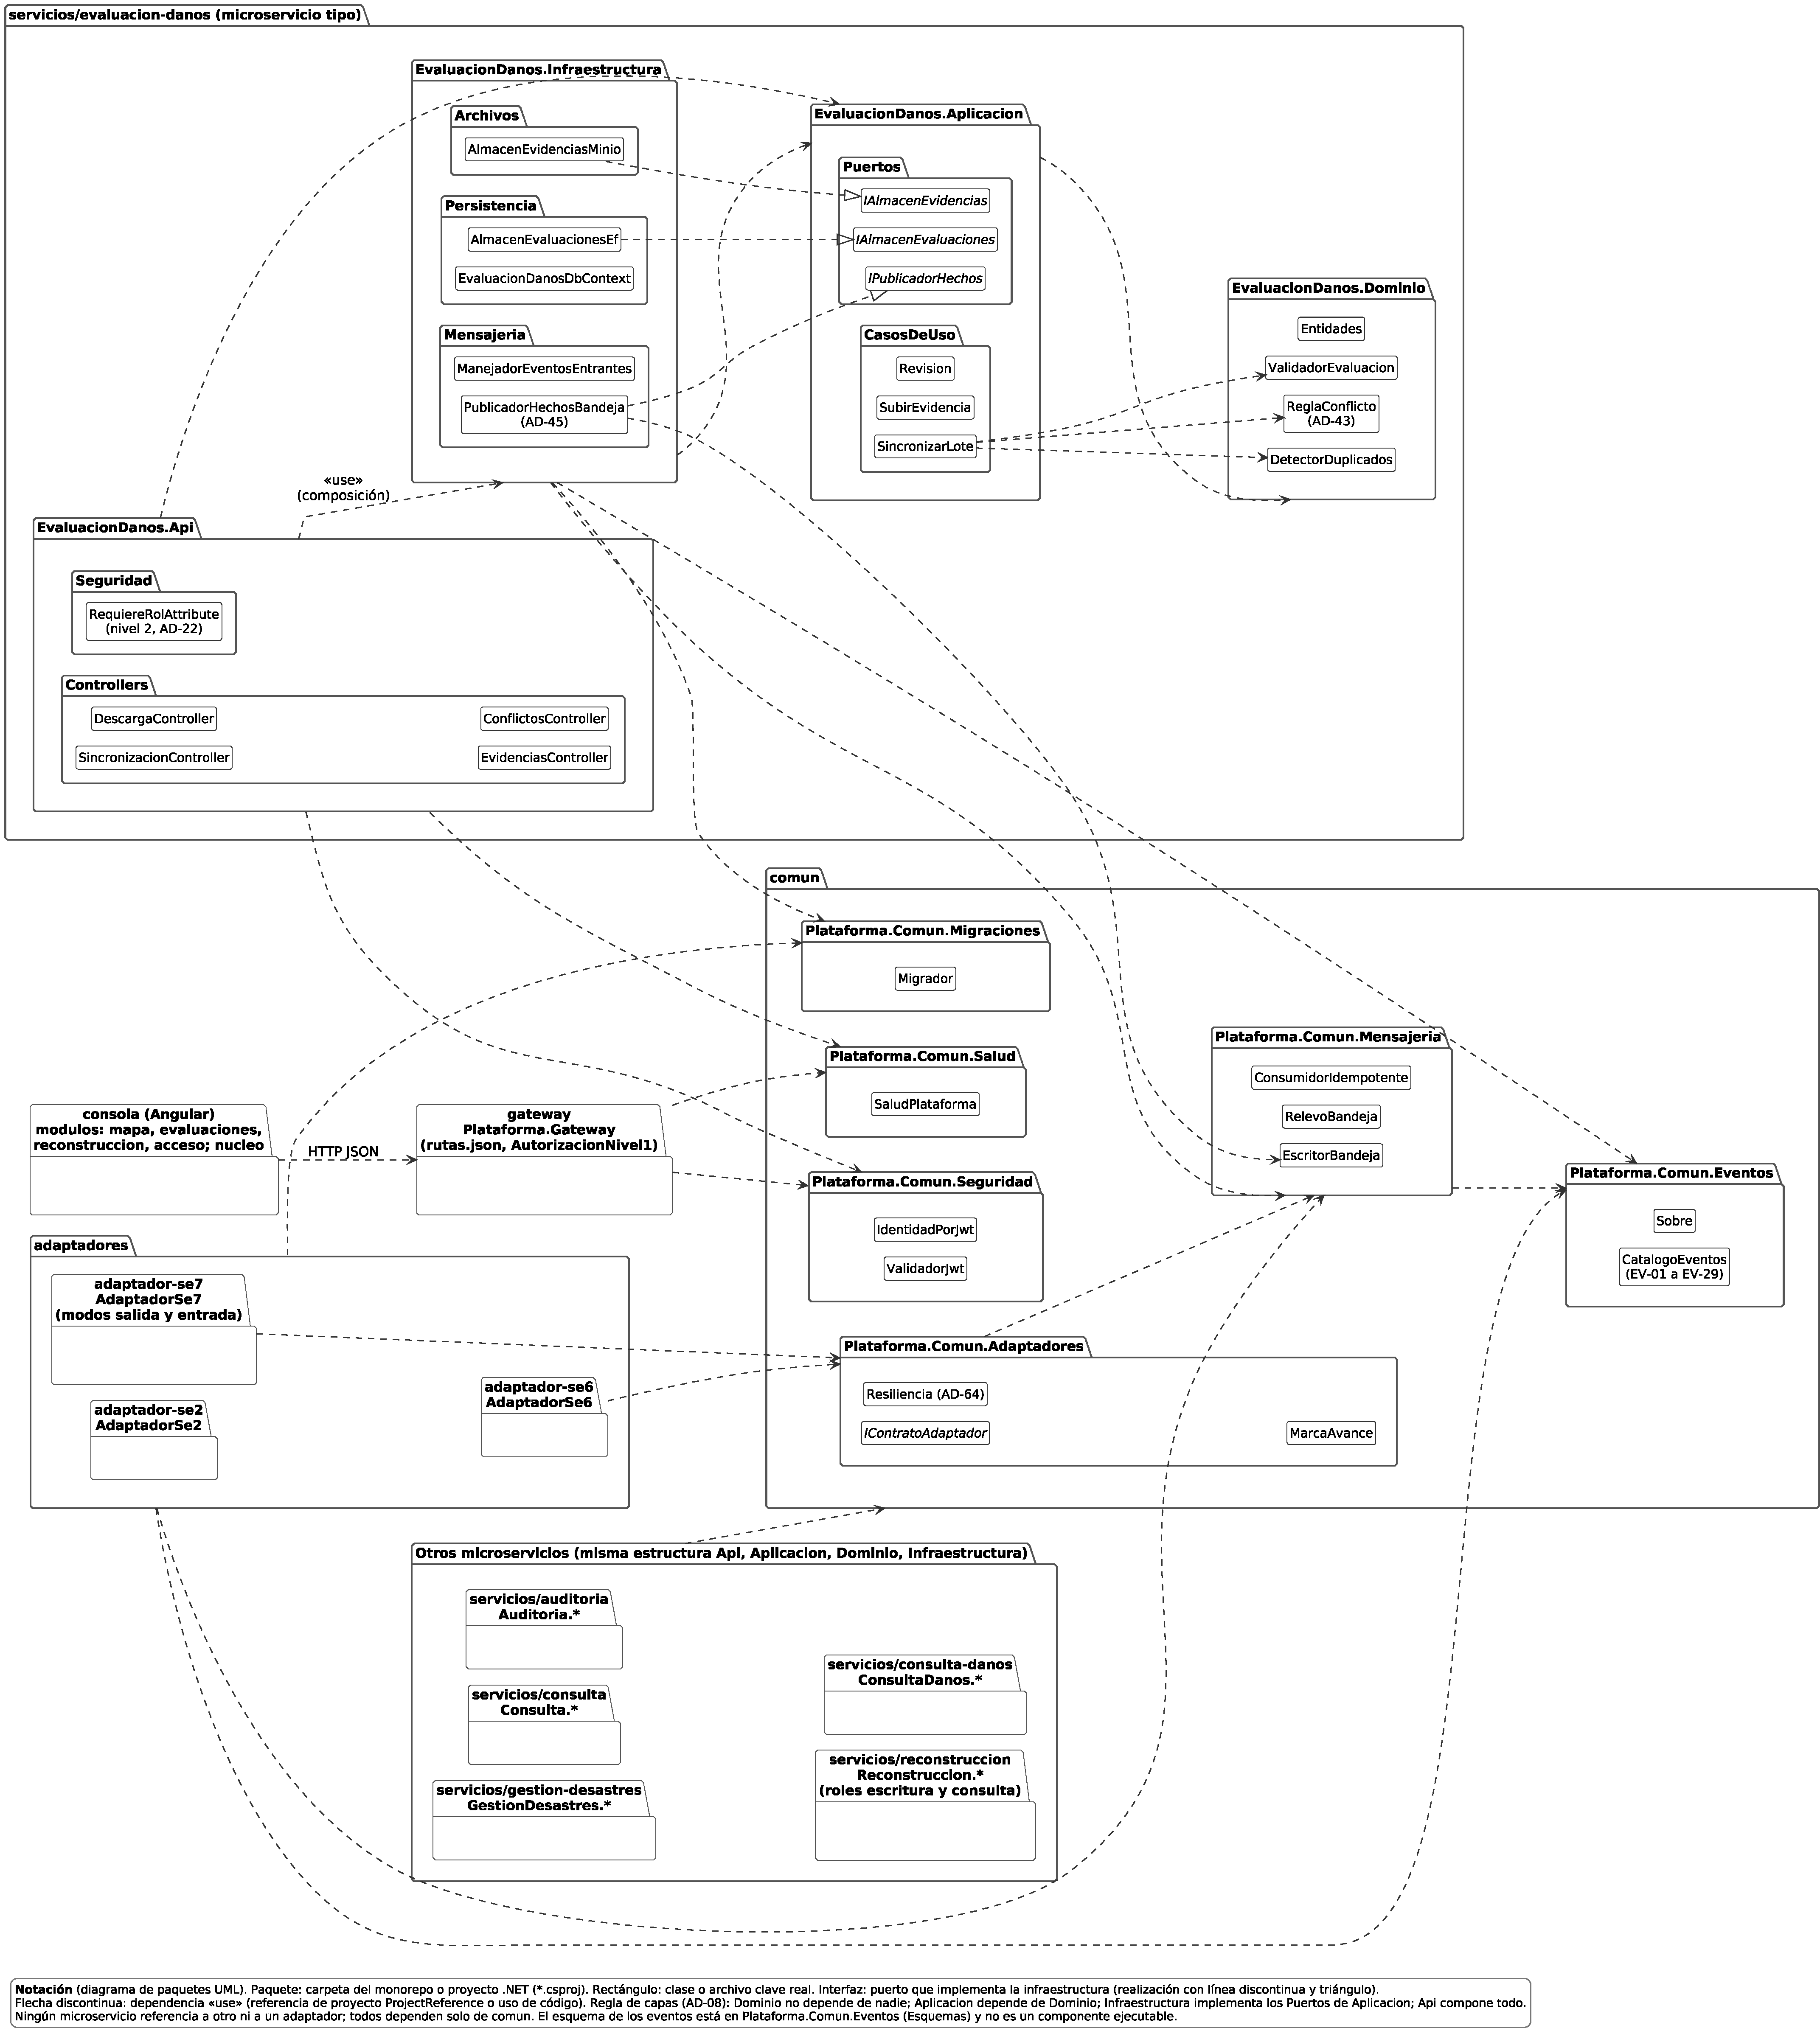
\includegraphics[width=\linewidth,height=0.92\textheight,keepaspectratio]{figuras/vista_implementacion}
\caption{Vista de implementación. Diagrama de paquetes UML del microservicio tipo, el módulo común,
los adaptadores y los demás microservicios.}
\label{fig:vista-implementacion}
\end{figure}

\begin{figure}[H]
\centering
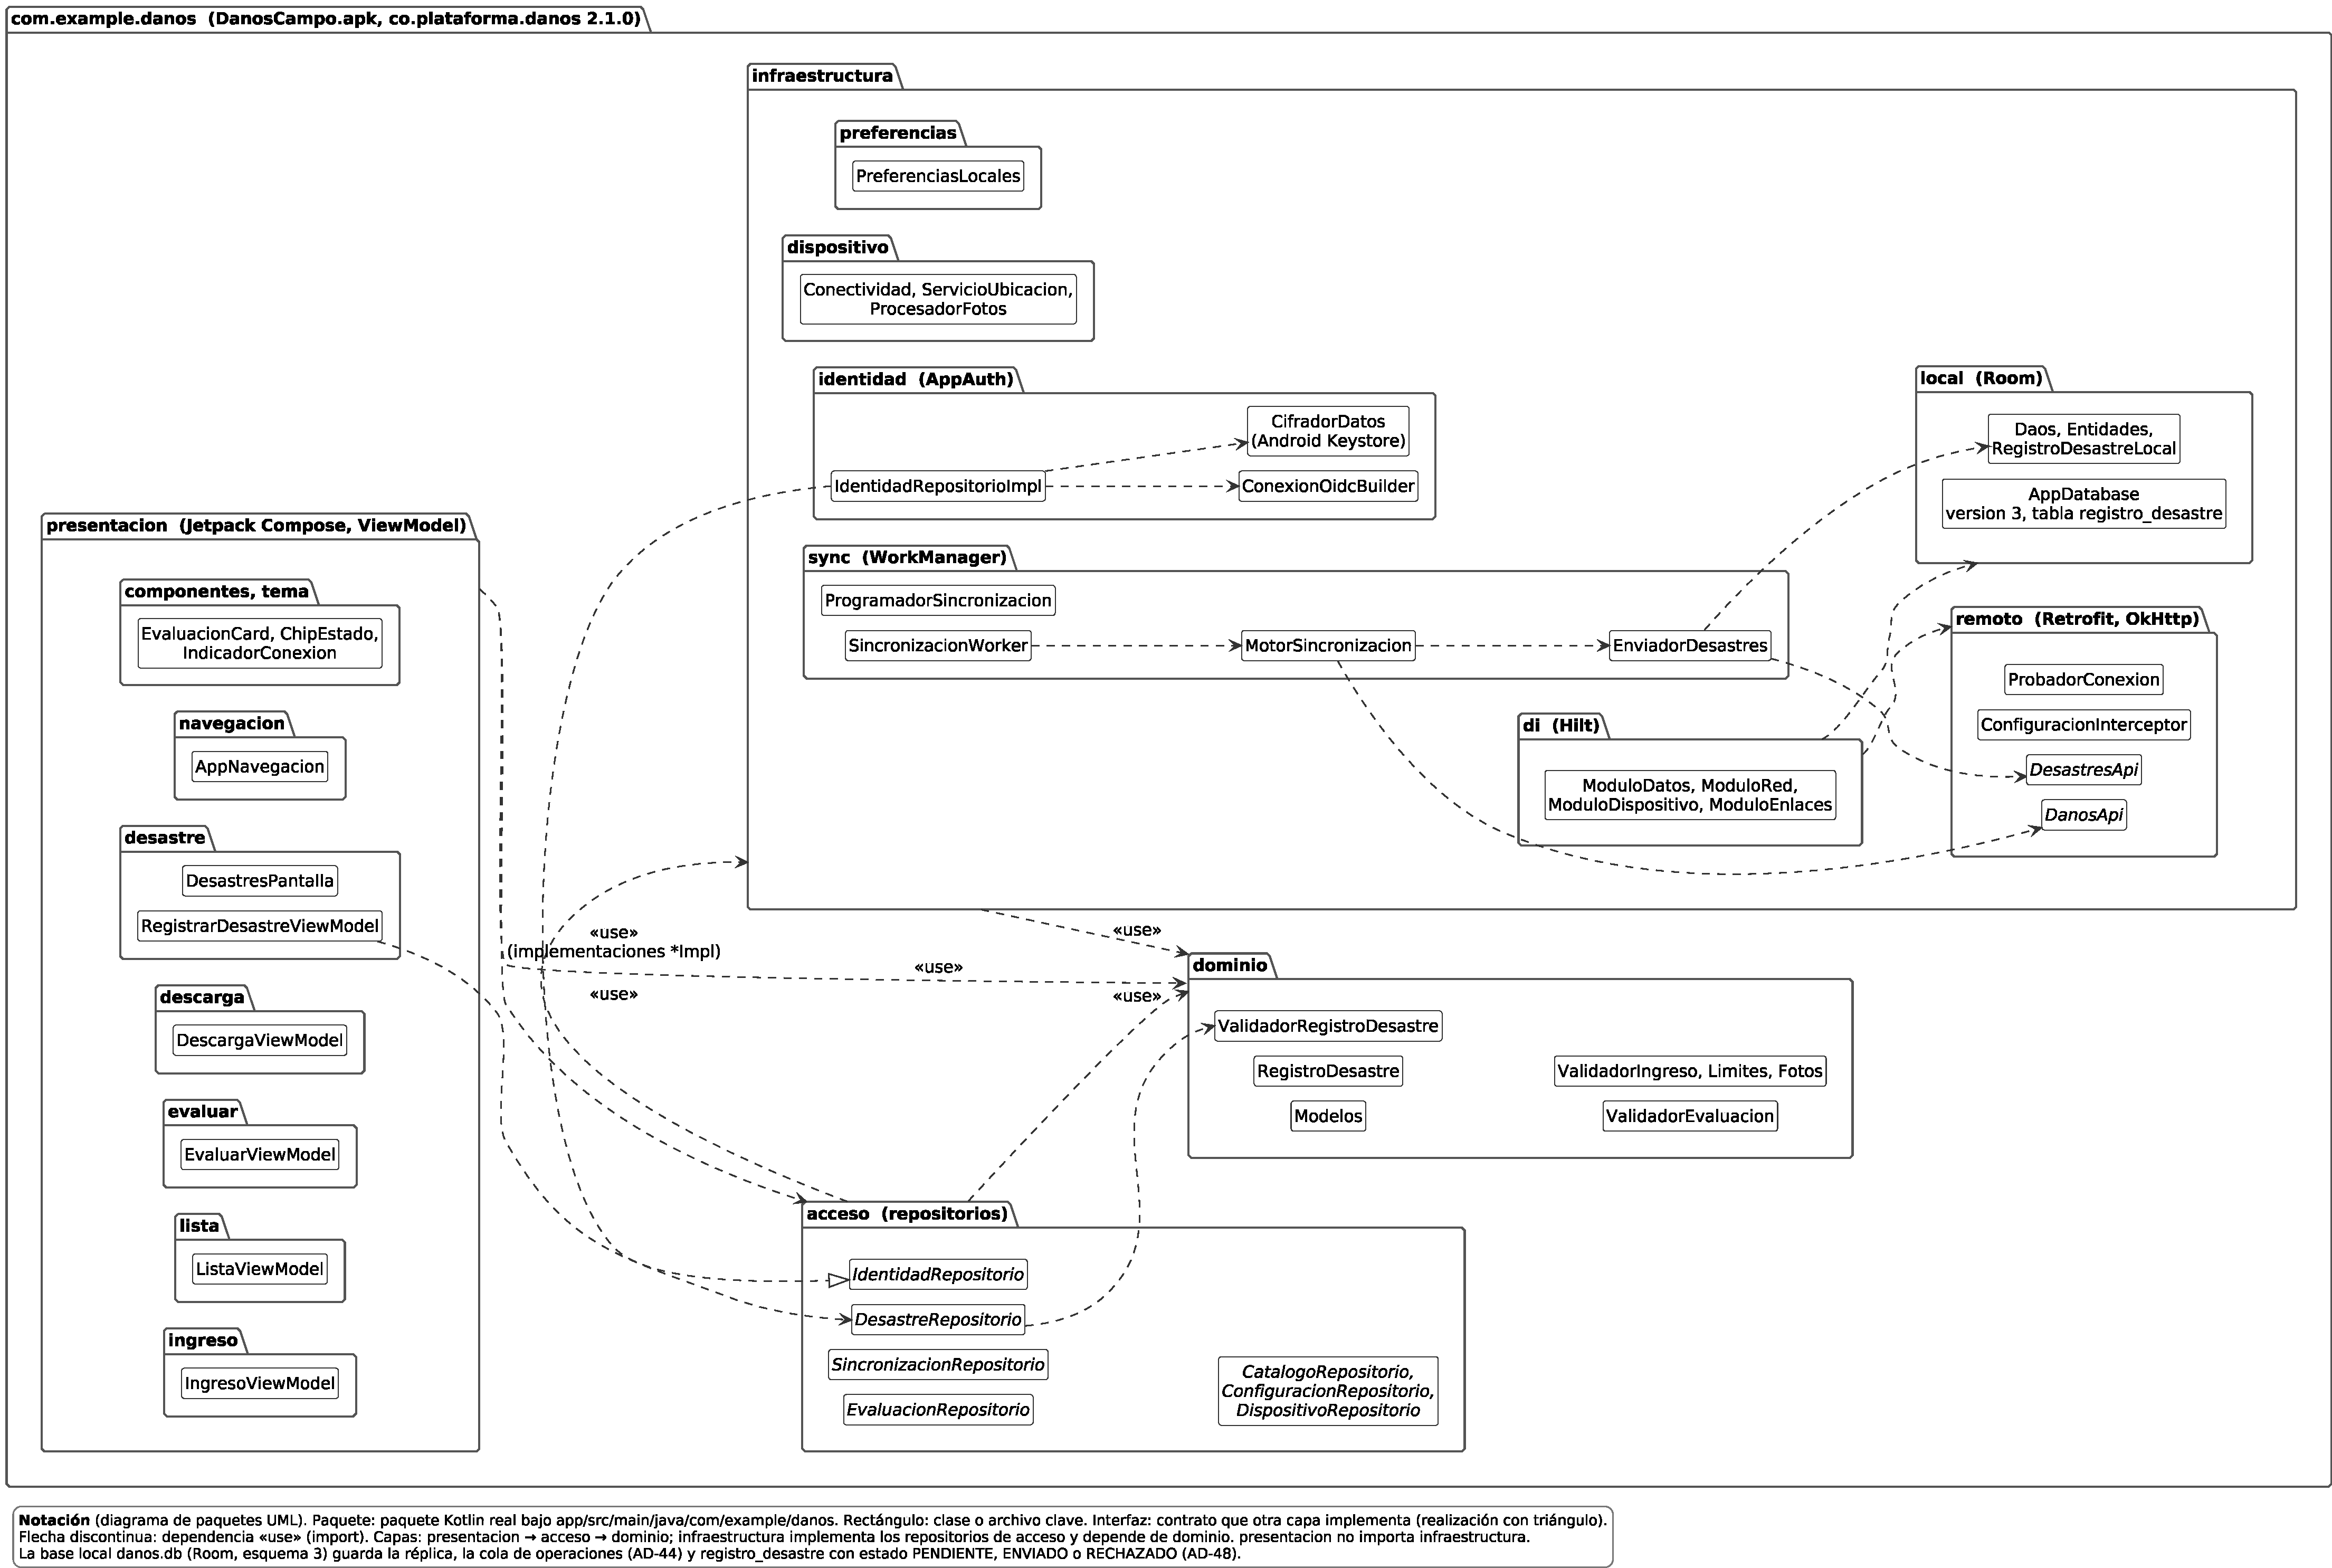
\includegraphics[width=\linewidth,height=0.8\textheight,keepaspectratio]{figuras/vista_implementacion_movil}
\caption{Vista de implementación. Diagrama de paquetes UML del cliente móvil.}
\label{fig:vista-implementacion-movil}
\end{figure}

El SAD 1.1 nombraba cuatro capas: presentación, acceso, dominio e infraestructura (AD-08). En el
código la capa de acceso se reparte entre dos proyectos: los controladores y la autorización de la
petición están en \texttt{*.Api}, y los casos de uso con sus puertos están en
\texttt{*.Aplicacion}. El \cref{tab:equivalencia-capas} fija la equivalencia.

\begin{longtable}{L{3.0cm} L{4.4cm} L{8.4cm}}
\cabecera{3}{tab:equivalencia-capas}{Equivalencia entre las capas de AD-08 y los proyectos del
código}{\textbf{Capa del SAD} & \textbf{Proyecto o paquete} & \textbf{Contenido en el código}}
Presentación & Consola (\texttt{consola}), cliente móvil (\texttt{presentacion}) y páginas Razor de
\texttt{ConsultaDanos.\br{}Api} & Pantallas de los clientes. En cada microservicio, los contratos de
petición y respuesta (\texttt{Presenters}, \texttt{Dtos.cs}) \\
Acceso & \texttt{*.Api} y \texttt{*.Aplicacion} & \texttt{*.Api}: \texttt{Controllers},
\texttt{Program.cs}, validación del token (nivel 2, AD-22) y reglas de dominio de la petición, por
ejemplo \texttt{EvaluacionDanos.\br{}Api/\br{}Seguridad}. \texttt{*.Aplicacion}: \texttt{CasosDeUso},
\texttt{Puertos} y \texttt{Hechos} \\
Dominio & \texttt{*.Dominio} & Entidades y reglas, por ejemplo \texttt{ReglaConflicto.\br{}cs} (AD-43),
\texttt{CicloDeVida.\br{}cs} (AD-07, AD-47), \texttt{MaquinaEstadosProyecto.\br{}cs} y
\texttt{Jurisdiccion.\br{}cs} \\
Infraestructura & \texttt{*.\br{}Infraestructura} y \texttt{Plataforma.\br{}Comun.\br{}*} & \texttt{Persistencia}
(contexto de datos, migraciones, historial), \texttt{Mensajeria} (manejadores de eventos y
publicador de la bandeja), \texttt{Archivos} (almacén de objetos) y \texttt{Registro.cs} \\
\end{longtable}

\begin{longtable}{L{4.2cm} L{11.6cm}}
\cabecera{2}{tab:paquetes}{Contenido de los paquetes de la vista de implementación}{\textbf{Proyecto
o paquete} & \textbf{Contenido}}
\texttt{Plataforma.\br{}Comun.\br{}Eventos} & \texttt{CatalogoEventos} (EV-01 a EV-29 y sus claves de ruteo),
\texttt{Sobre}, \texttt{Enumeraciones} y los esquemas JSON \texttt{EV-nn.v1.json} (AD-09). \\
\texttt{Plataforma.\br{}Comun.\br{}Mensajeria} & \texttt{ConexionBus}, \texttt{EscritorBandeja},
\texttt{RelevoBandeja}, \texttt{ConsumidorIdempotente} y \texttt{ValidadorContrato} (AD-02,
AD-45). \\
\texttt{Plataforma.\br{}Comun.\br{}Adaptadores} & \texttt{IContratoAdaptador}, \texttt{MarcaAvance},
\texttt{MonitorCircuito}, \texttt{EstadoIntegracion} y \texttt{Resiliencia} (AD-05, AD-09, AD-14,
AD-64). \\
\texttt{Plataforma.\br{}Comun.\br{}Seguridad} & \texttt{IdentidadPorJwt}: validación del token en cada
microservicio (AD-22, AD-49). \\
\texttt{Plataforma.\br{}Comun.\br{}Migraciones} y \texttt{Plataforma.\br{}Comun.\br{}Salud} & Migrador común y
sondeos de salud \texttt{/salud/vivo} (AD-24, AD-53). \\
\texttt{GestionDesastres.\br{}*}, \texttt{EvaluacionDanos.\br{}*}, \texttt{Reconstruccion.\br{}*},
\texttt{Consulta.*}, \texttt{ConsultaDanos.\br{}*}, \texttt{Auditoria.*} & Los seis microservicios
implementados, cada uno con \texttt{Api}, \texttt{Aplicacion}, \texttt{Dominio} e
\texttt{Infraestructura}, y sus proyectos de pruebas \texttt{*.Pruebas} e \texttt{*.Integracion}.
Consulta del Programa está dentro de \texttt{Reconstruccion.\br{}*} (AD-42). \\
\texttt{AdaptadorSe2}, \texttt{AdaptadorSe6}, \texttt{AdaptadorSe7} & Cliente del sistema externo,
traductor al evento canónico, cortacircuitos y marca de avance (AD-03, AD-14, AD-36). \\
\texttt{adaptador-\br{}se8-\br{}jee} (Java) & Paquetes \texttt{contrato} (\texttt{ContratoAdaptador},
\texttt{Sobre}, \texttt{ValidadorContrato}), \texttt{traduccion}, \texttt{resiliencia}
(\texttt{Cortacircuitos}, \texttt{EjecutorResiliente}), \texttt{cliente}, \texttt{persistencia},
\texttt{consumo}, \texttt{nucleo}, \texttt{jee} (EJB y CDI) y \texttt{api}, y el módulo
\texttt{migrador} con Flyway (AD-03, AD-14, AD-36, AD-45, AD-66). \\
\texttt{Plataforma.\br{}Gateway} & Catálogo \texttt{rutas.json}, validación del token (nivel 1) y
priorización por clase de tráfico (AD-04, AD-19). \\
\texttt{danos/app}, paquete \texttt{com.\br{}example.\br{}danos} & \texttt{presentacion} (\texttt{ingreso},
\texttt{descarga}, \texttt{lista}, \texttt{evaluar}, \texttt{desastre}, \texttt{navegacion}),
\texttt{acceso} (repositorios, entre ellos \texttt{DesastreRepositorio}), \texttt{dominio}
(\texttt{Modelos}, \texttt{RegistroDesastre}, \texttt{ValidadorEvaluacion}) e
\texttt{infraestructura}: \texttt{local} (\texttt{AppDatabase}, \texttt{Daos},
\texttt{RegistroDesastreLocal}), \texttt{sync} (\texttt{MotorSincronizacion},
\texttt{SincronizacionWorker}, \texttt{EnviadorDesastres}), \texttt{remoto} (\texttt{DanosApi},
\texttt{DesastresApi}), \texttt{identidad} (\texttt{ConexionOidcBuilder}), \texttt{dispositivo}
(\texttt{ServicioUbicacion}, \texttt{ProcesadorFotos}), \texttt{preferencias} y \texttt{di}
(AD-31, AD-44, AD-48). \\
\end{longtable}

El \cref{tab:que-se-modifica} indica los paquetes que se modifican ante los tres cambios previstos.
Es la verificación de las medidas de QA-09 y QA-10 sobre esta vista.

\begin{longtable}{L{3.8cm} L{4.6cm} L{4.6cm} L{2.6cm}}
\cabecera{4}{tab:que-se-modifica}{Qué se modifica para incorporar un sistema externo, un tipo de
desastre o un microservicio}{\textbf{Cambio} & \textbf{Qué se agrega o se modifica} & \textbf{Qué no
se modifica} & \textbf{Escenario}}
Incorporar un sistema externo & Se agrega un proyecto \texttt{AdaptadorSe9}, que implementa
\texttt{IContratoAdaptador}, y su cola de salida en \texttt{definiciones.\br{}json} & Los doce
microservicios, los proyectos \texttt{Plataforma.\br{}Comun.\br{}*} y los adaptadores existentes & QA-09: 0
componentes existentes modificados \\
Incorporar un tipo de desastre & Se agrega una entrada al catálogo de tipos, con su perfil de ciclo
de vida y sus criterios, por medio de la API de catálogos & Ningún paquete. No hay cambio de código
ni redespliegue & QA-10: 0 componentes modificados o redesplegados \\
Incorporar un microservicio & Se agrega un paquete con las cuatro capas, su almacén, su cola en el
bus y sus rutas en el API Gateway & Los microservicios existentes. Los eventos que el microservicio
nuevo consume ya se publican & QA-10 y QA-05 (CON-4) \\
\midrule
Evidencia: se incorporó SE-8 (19 de noviembre de 2026) & El proyecto Maven
\texttt{adaptador-\br{}se8-\br{}jee} (76 archivos) y el simulador \texttt{sim-se8} (6). Dos enlaces de
\texttt{q.salida.se8} en \texttt{definiciones.\br{}json} y su generador, tres servicios en el compose,
un manifiesto de Kubernetes y una prueba de humo & Los seis microservicios, los proyectos
\texttt{Plataforma.\br{}Comun.\br{}*}, el gateway, la consola y los adaptadores de SE-2, SE-6 y SE-7:
0 líneas cambiadas & QA-09: medida cumplida, 0 componentes existentes modificados \\
\end{longtable}

El \texttt{git diff --stat} del commit que incorporó SE-8 muestra 89 archivos con 7\,131 líneas
agregadas y 1 borrada. De ellos, 84 son nuevos: el adaptador (76), el simulador (6), el manifiesto
\texttt{adaptador-\br{}se8.\br{}yaml} y la prueba \texttt{prueba-se8.sh}. Los 5 modificados son de
despliegue y solo agregan líneas, salvo una: \texttt{definiciones.\br{}json} (+16),
\texttt{generar\_\br{}definiciones.py} (+3 $-$1, la lista de enlaces de \texttt{q.salida.se8}),
\texttt{docker-\br{}compose.\br{}yml} (+69), \texttt{aplicar.sh} (+7) y \texttt{kustomization.\br{}yaml} (+1). Ningún
archivo de \texttt{servicios/}, \texttt{comun/}, \texttt{gateway/}, \texttt{consola/} ni de los
adaptadores existentes aparece en el diff. La medida vale aunque el adaptador nuevo esté en otra pila
(Jakarta EE): el contrato común es el esquema del evento canónico, no una biblioteca .NET (AD-09).

\subsection{Vista de casos de uso}
\label{sec:vista-casos-uso}

La quinta vista del modelo 4+1 muestra cómo los elementos de las otras cuatro vistas colaboran para
realizar los casos de uso. La \cref{fig:casos-uso} presenta los diez casos de uso primarios del SRS
con sus actores y el caso de registro del desastre en campo. A continuación se especifican cinco
casos de uso. Los tres primeros corresponden a los escenarios de operación EO-1, EO-3 y EO-4 del
SRS. Se eligen porque cada uno recorre una combinación distinta de mecanismos: la cadena de
integración y notificación (QA-07, QA-08, QA-09), la tolerancia al fallo de un sistema externo
(QA-01) y la sincronización sin conexión (QA-14). CU-4 recorre el registro en campo con
identificador del cliente (AD-48). CU-5 recorre la reconstrucción (EO-5). CU-1 a CU-4 se acompañan de
un diagrama de secuencia UML, y las secuencias de CU-5 están en el documento de diseño del módulo de
Reconstrucción \cite{diseno-rc}. CU-1 y CU-2 recorren elementos que quedan como diseño (SE-1, SE-3,
Consolidación y Notificación, L-06). CU-3, CU-4 y CU-5 están implementados de punta a punta.

El \cref{tab:actores-cu} lista los actores de esta vista. SE-6 y SE-7 son actores distintos: SE-6 es
el sistema financiero y recibe el presupuesto y los costos, y SE-7 es el sistema de proyectos, que
recibe las obras y además reporta avance y contratista. El administrador, el auditor y el responsable
de proyecto son roles de la plataforma (\cref{tab:apis}).

\begin{longtable}{L{3.9cm} L{3.0cm} L{8.9cm}}
\cabecera{3}{tab:actores-cu}{Actores de la vista de casos de uso}{\textbf{Actor} & \textbf{Tipo o rol} &
\textbf{Participación}}
Organismo de respuesta & \texttt{organismo} & Actualiza el desastre y consulta su estado (CU-1, CU-2).
Lo registra en campo (CU-4) \\
Autoridad & \texttt{autoridad} & Registra desastres en campo (CU-4). Crea, asigna y aprueba proyectos
de su jurisdicción (CU-5) \\
Evaluador de campo & \texttt{evaluador} & Registra evaluaciones sin conexión (CU-3) \\
Operador de la plataforma & \texttt{operador} & Resuelve conflictos y duplicados (CU-3) \\
Administrador & \texttt{administrador} & Administra los catálogos de tipos de desastre, los perfiles
de ciclo de vida y los tipos de activo (FP-01, FP-06, QA-10) \\
Auditor & \texttt{auditor} & Consulta el rastro de auditoría y el historial de los proyectos, sin
modificar nada (QA-13, QA-15, CU-5) \\
Responsable de proyecto & \texttt{responsable-\br{}proyecto} & Inicia la ejecución y registra avance y
costos del proyecto que tiene asignado (CU-5) \\
Ciudadano & Portal público & Consulta información pública y registra solicitudes de ayuda (FP-02,
«diseño») \\
SE-1 & Sistema externo & Origina el registro automático de un desastre (CU-1) \\
SE-2 & Sistema externo & Aporta capas y zonas geográficas \\
SE-3 & Sistema externo & Sistema hospitalario cuya caída se analiza en CU-2 \\
SE-4 y SE-5 & Sistemas externos & Recursos, y personas afectadas (FP-07 y FP-10, «diseño») \\
SE-6 & Sistema externo & Sistema financiero: recibe presupuesto y costos (EV-18, EV-19 y EV-20, CU-5) \\
SE-7 & Sistema externo & Sistema de proyectos: recibe las obras (EV-18 y EV-20) y reporta avance y
contratista (EV-24, CU-5) \\
SE-8 & Sistema externo & Entrega las alertas y devuelve el acuse (CU-1) \\
Proveedor de identidad & Sistema externo & Autentica a los usuarios de todos los clientes (CU-4, AD-49) \\
\end{longtable}

La \cref{fig:casos-uso} todavía agrupa a SE-6 y SE-7 en un solo actor y no dibuja al administrador, al
auditor ni al responsable de proyecto. El \cref{tab:actores-cu} es la lista vigente.

\begin{figure}[H]
\centering
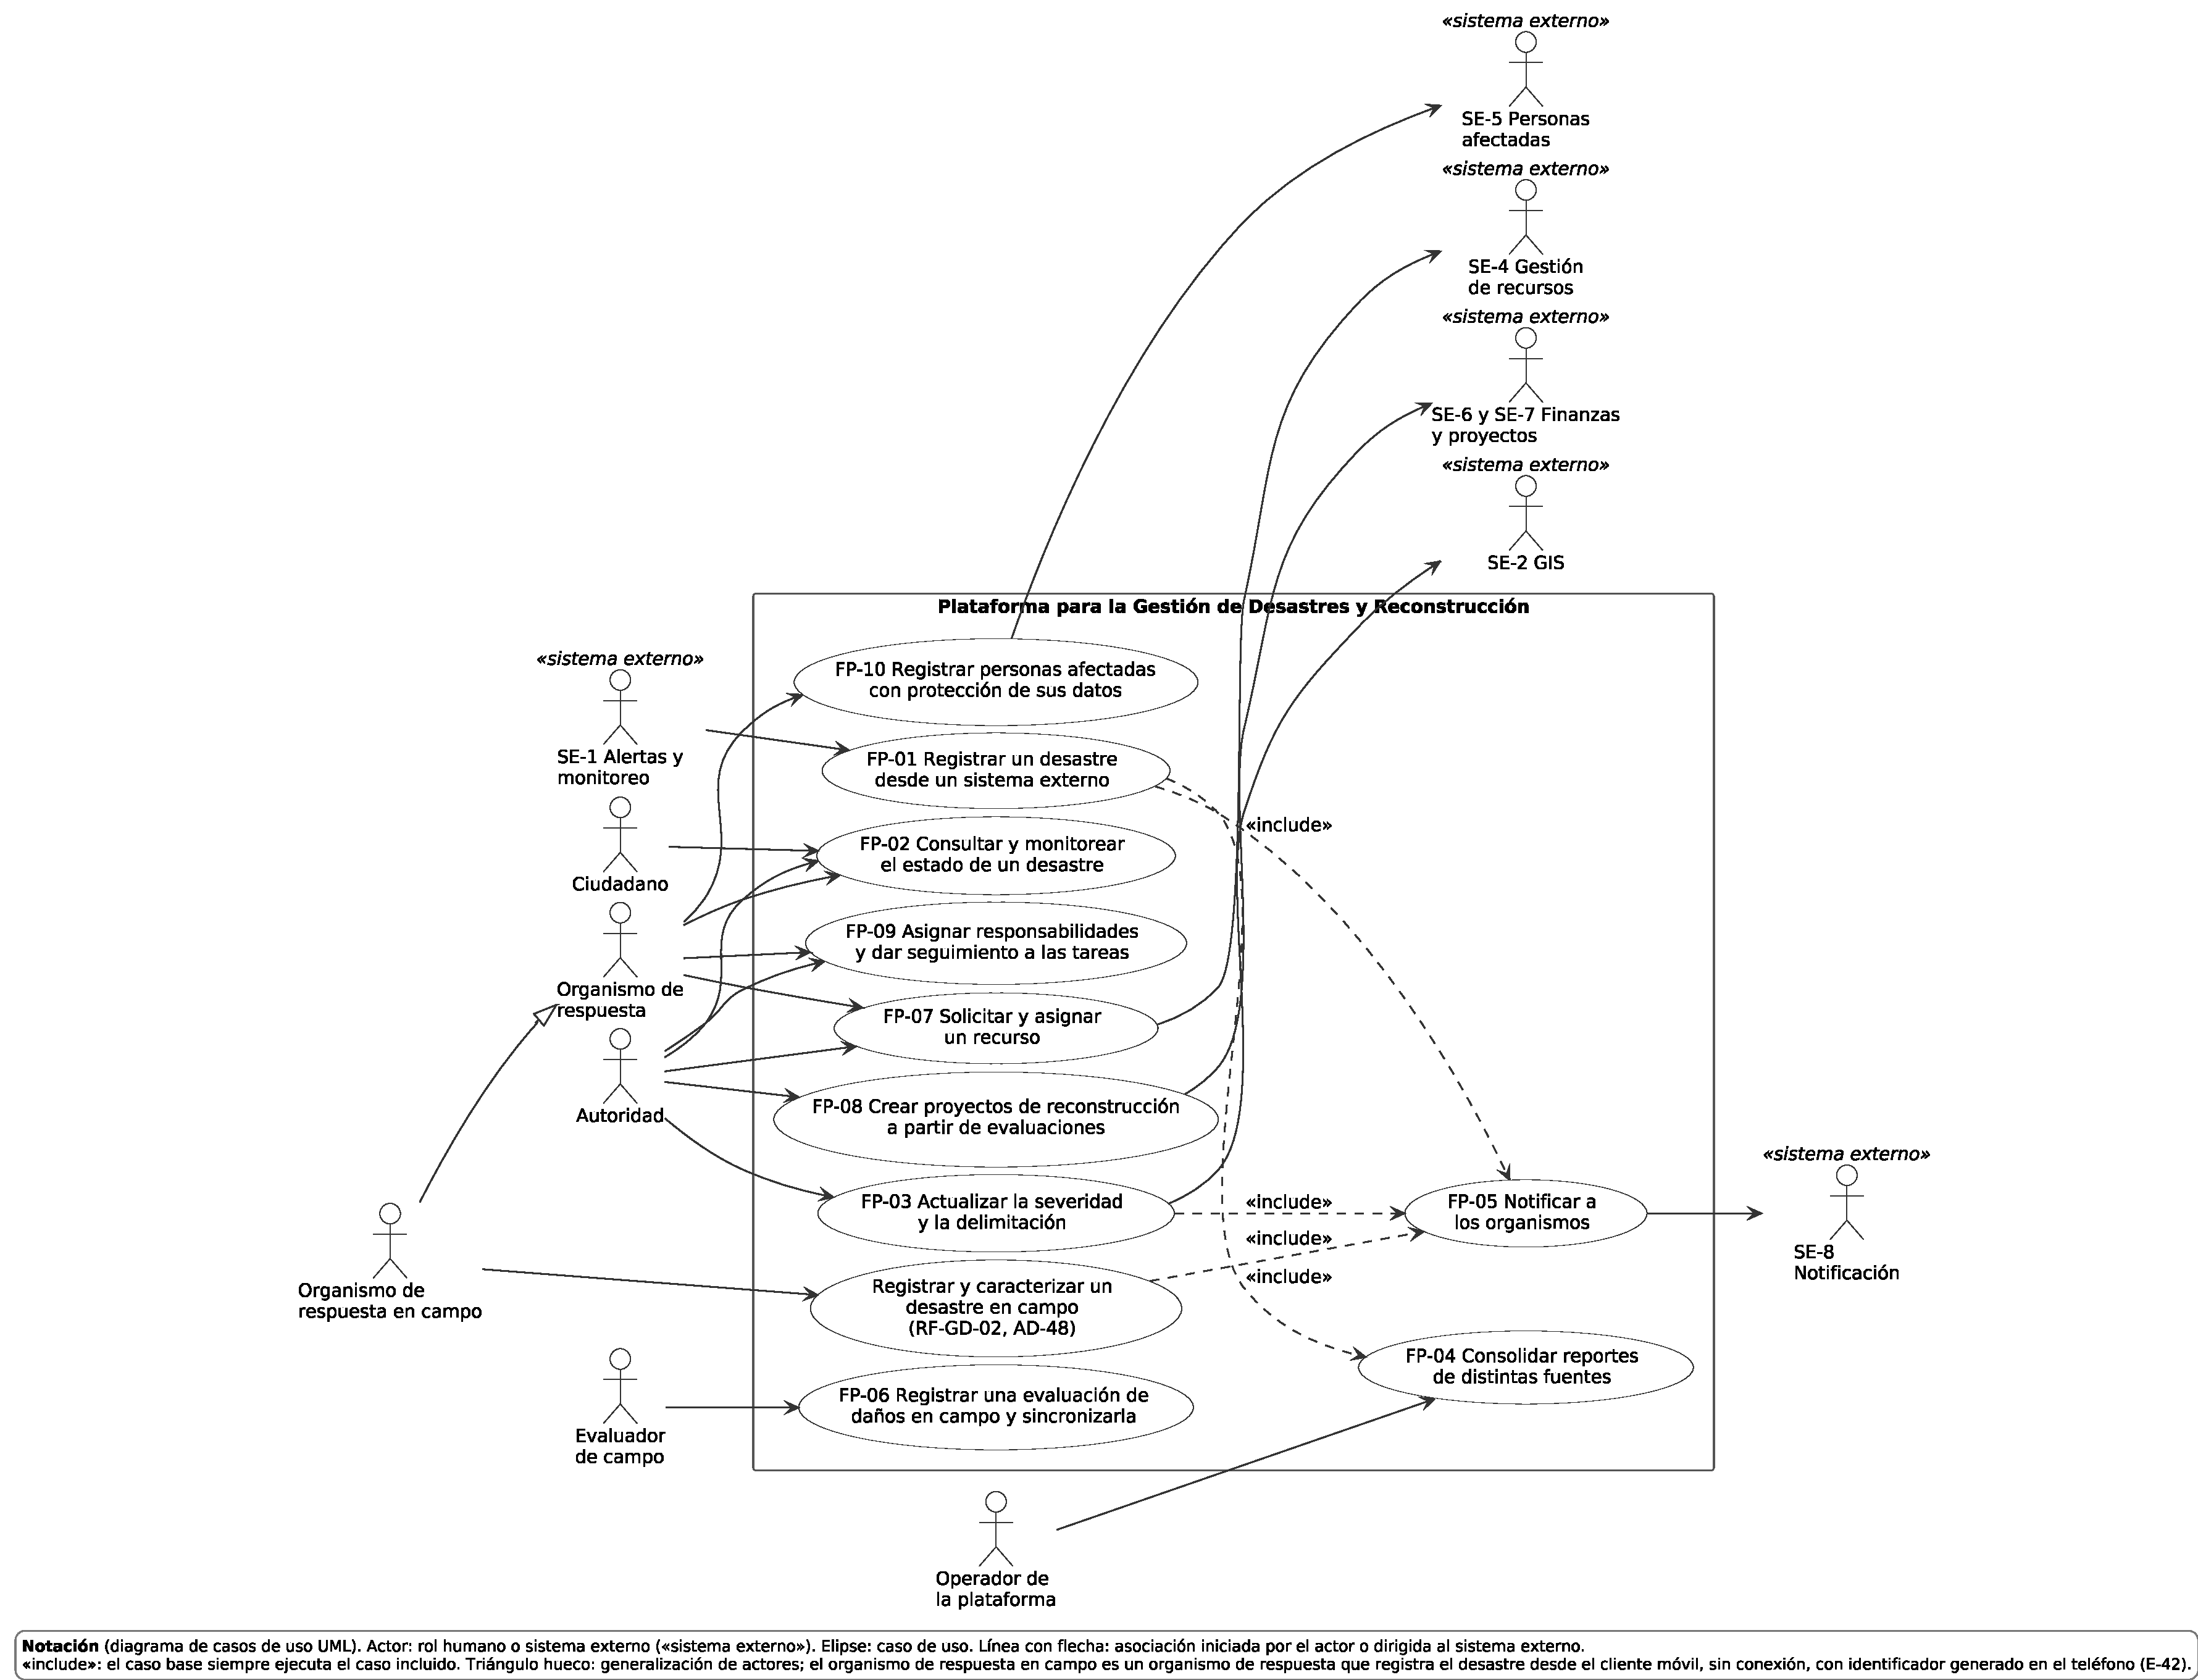
\includegraphics[width=0.86\linewidth]{figuras/casos_uso}
\caption{Diagrama de casos de uso de la funcionalidad primaria (FP-01 a FP-10) y del registro del
desastre en campo (CU-4).}
\label{fig:casos-uso}
\end{figure}

\subsubsection{Caso de uso CU-1: inicio de una emergencia (EO-1)}

\begin{longtable}{L{3.2cm} L{12.6cm}}
\cabecera{2}{tab:cu1}{Especificación del caso de uso CU-1}{\textbf{Campo} & \textbf{Contenido}}
Nombre & Registrar un desastre a partir de un sistema externo y notificarlo \\
Casos de uso primarios & FP-01, FP-04, FP-05 \\
Actores & SE-1 (primario), organismo responsable, SE-8 \\
Disparador & SE-1 detecta un fenómeno y envía un aviso \\
Precondiciones & El adaptador de SE-1 está desplegado. El tipo de fenómeno existe en el catálogo de
tipos (RN-1) \\
Flujo principal &
1. El adaptador de SE-1 recibe el aviso, lo traduce al evento canónico y publica EV-01.\newline
2. Consolidación descarta los reenvíos por clave de origen, correlaciona el reporte por ventana de
espacio y tiempo y publica EV-02 con la procedencia.\newline
3. Gestión de Desastres valida el tipo contra el catálogo, crea el desastre en estado Detectado y
publica EV-03.\newline
4. Notificación resuelve las suscripciones y envía la alerta por el adaptador de SE-8. Cuando recibe
el acuse, publica EV-07.\newline
5. Consulta actualiza sus proyecciones y Auditoría registra los eventos.\newline
6. El organismo responsable completa la información y cambia el estado del desastre por el API
Gateway. Gestión de Desastres publica EV-06 \\
Flujos alternativos &
2a. La correlación no alcanza la confianza configurada: el reporte queda pendiente y el operador lo
confirma o lo rechaza (AD-10).\newline
3a. El tipo no existe en el catálogo: el reporte se rechaza y queda registrado.\newline
4a. SE-8 no acusa en \qty{5}{\second}: la notificación queda pendiente y se reintenta (QA-08).\newline
6a. El organismo no es el responsable asignado: Gestión de Desastres rechaza la operación y
Auditoría registra el intento (QA-11) \\
Postcondiciones & El desastre existe con su procedencia. Cada notificación tiene un estado de
entrega. Los eventos EV-01, EV-02, EV-03, EV-06 y EV-07 están en el registro de auditoría \\
Escenarios de calidad & QA-07, QA-08, QA-09 \\
Decisiones & AD-03, AD-07, AD-09, AD-10, AD-11, AD-13, AD-21, AD-22 \\
\end{longtable}

En este caso de uso, SE-1 no conoce la plataforma, el adaptador no conoce los microservicios de
dominio y los microservicios no conocen a SE-1. Por eso la incorporación de un sistema externo no
modifica ningún microservicio (QA-09). La \cref{fig:seq-eo1} muestra la secuencia.

\begin{landscape}
\begin{figure}[p]
\centering
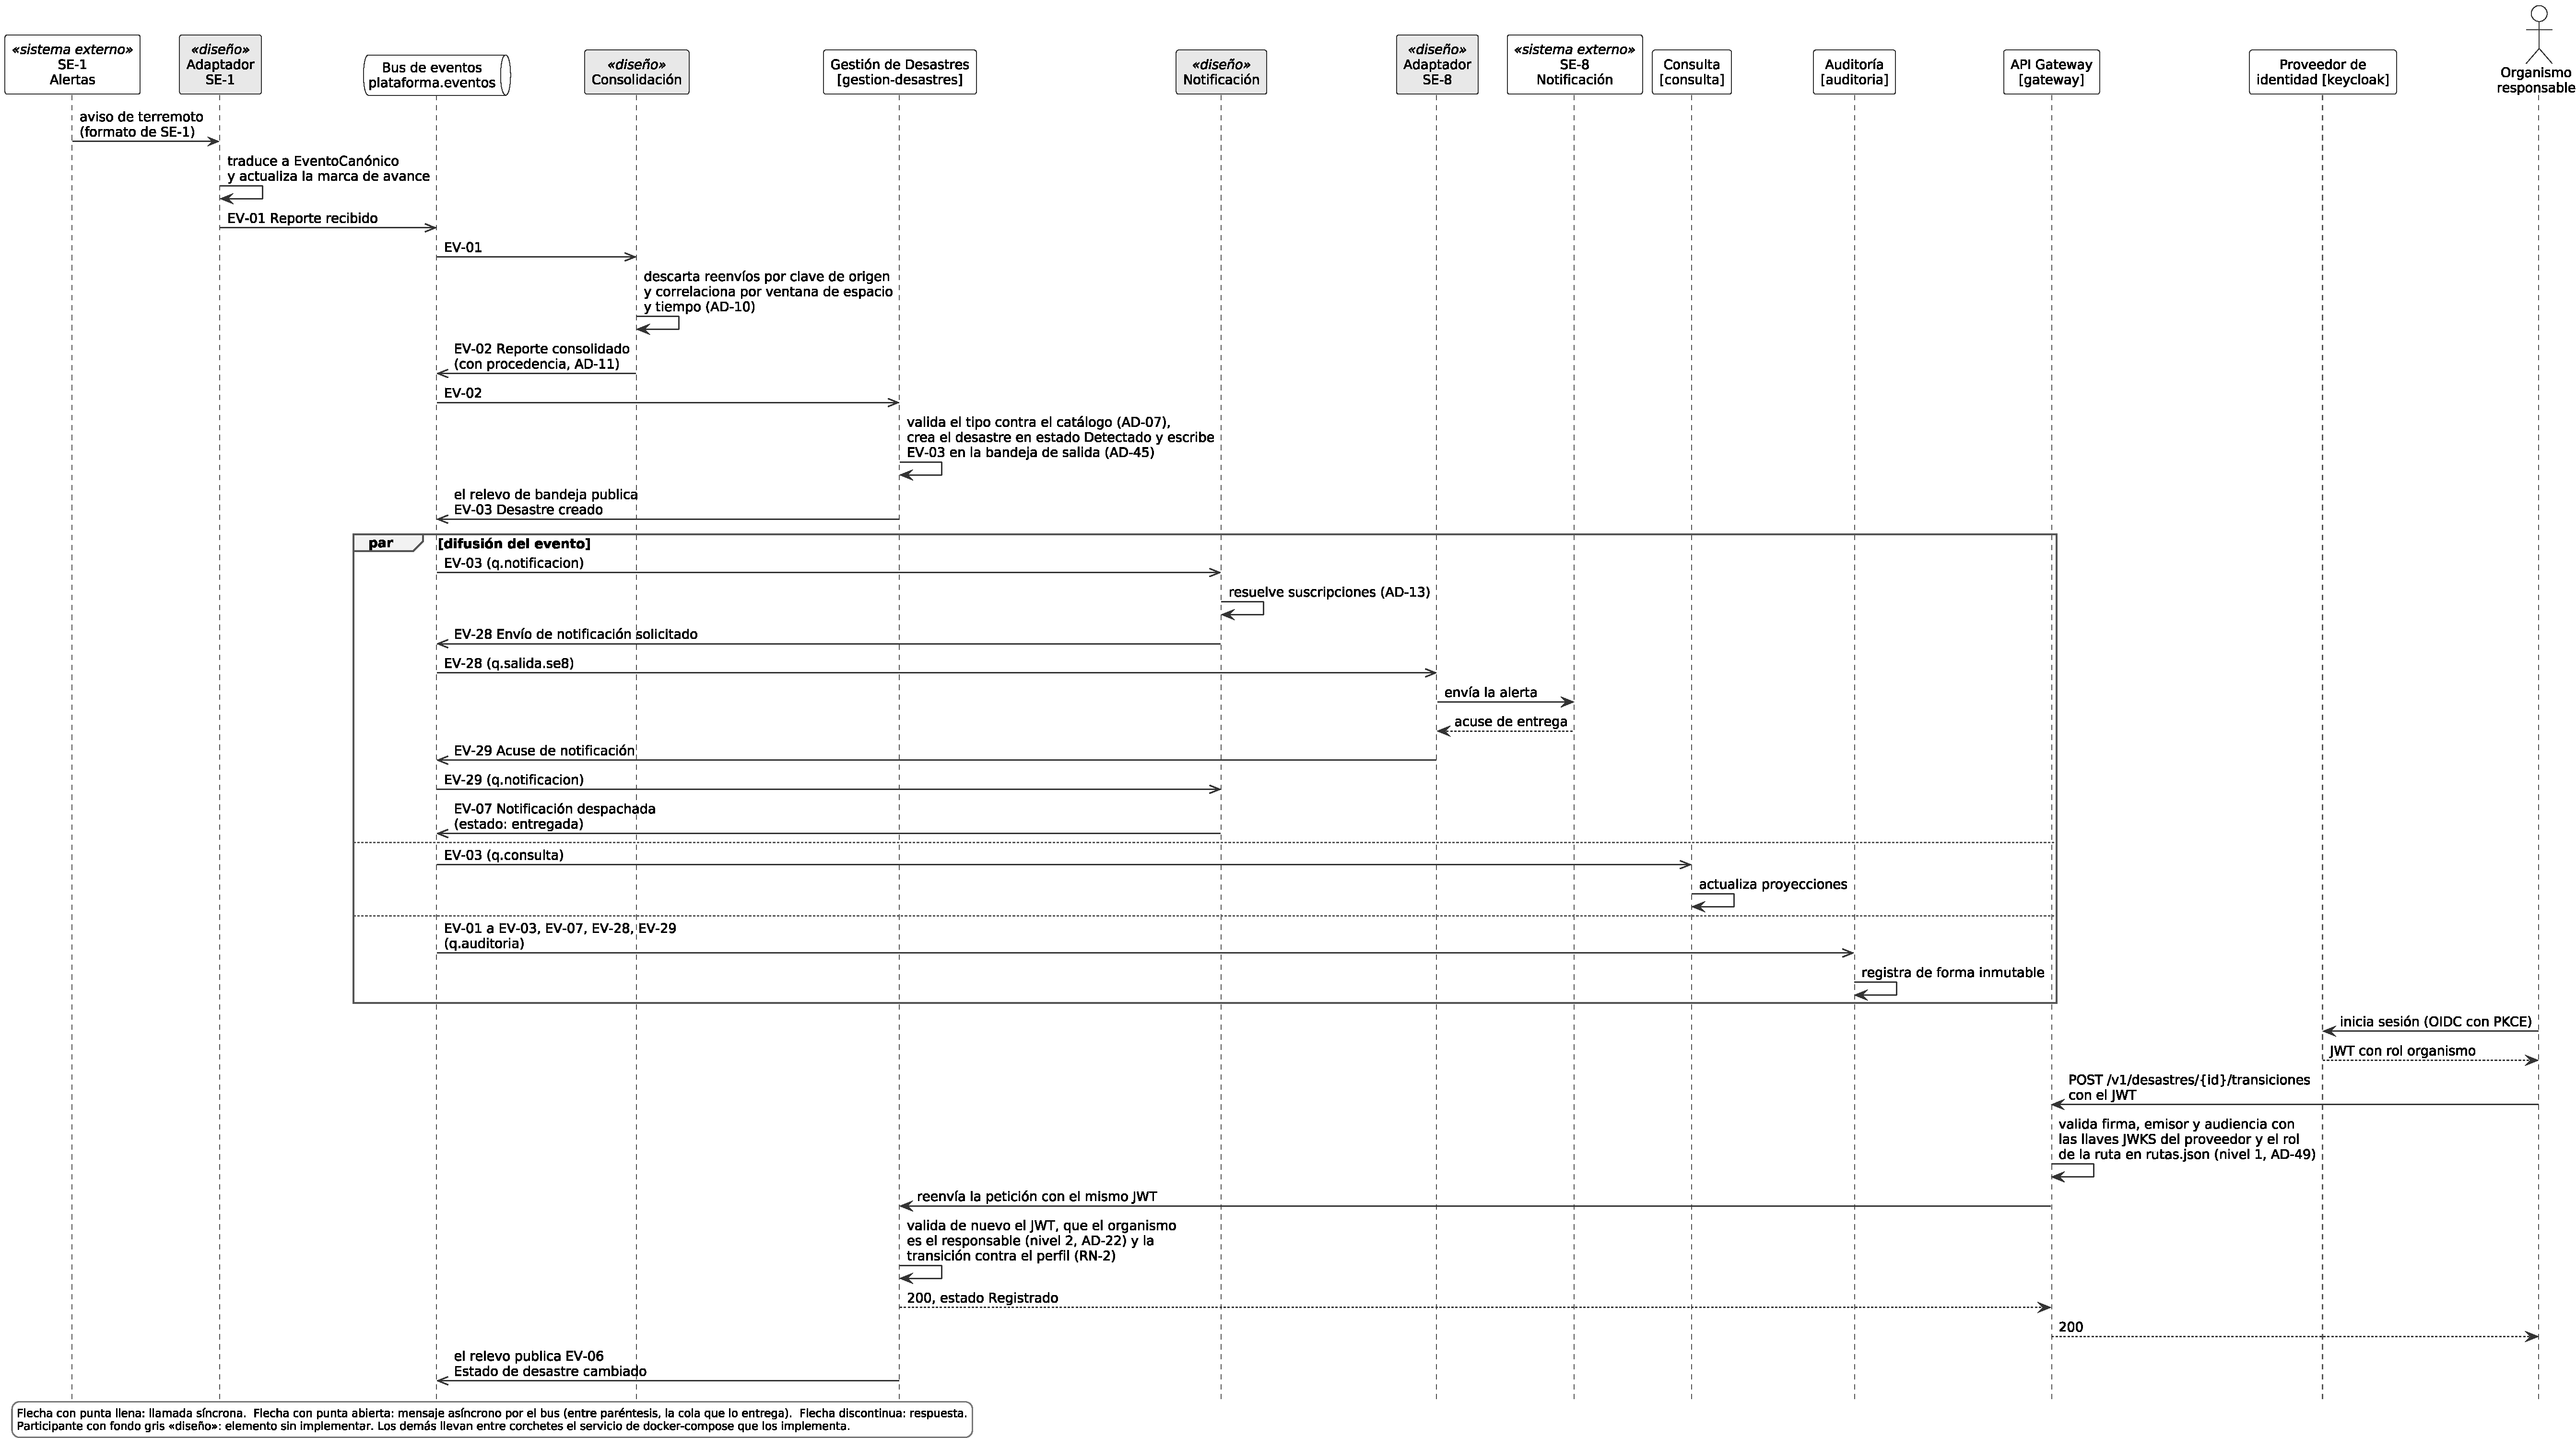
\includegraphics[width=\linewidth,height=0.86\textheight,keepaspectratio]{figuras/seq_eo1}
\caption{Diagrama de secuencia de CU-1: inicio de una emergencia (EO-1).}
\label{fig:seq-eo1}
\end{figure}
\end{landscape}

\subsubsection{Caso de uso CU-2: fallo de un sistema externo (EO-3)}

\begin{longtable}{L{3.2cm} L{12.6cm}}
\cabecera{2}{tab:cu2}{Especificación del caso de uso CU-2}{\textbf{Campo} & \textbf{Contenido}}
Nombre & Continuar la operación cuando SE-3 no responde y sincronizar cuando se restablece \\
Casos de uso primarios & FP-02 (consulta degradada). Los demás casos de uso continúan sin cambio \\
Actores & SE-3, organismo de respuesta \\
Disparador & SE-3 deja de responder: en una ventana de \qty{30}{\second}, con al menos tres llamadas
del adaptador, el \qty{100}{\percent} falla (AD-05, AD-64) \\
Precondiciones & Hay una emergencia activa. La proyección de consulta contiene un dato hospitalario
anterior, con su marca de tiempo \\
Flujo principal &
1. El cortacircuitos del adaptador de SE-3 se abre. El adaptador deja de invocar a SE-3.\newline
2. Los eventos dirigidos a SE-3 se acumulan en su cola de salida. Los microservicios que los
publican no esperan.\newline
3. El organismo consulta el estado del desastre. Consulta devuelve el último dato hospitalario con
su marca de tiempo.\newline
4. El registro de daños, de recursos y de tareas continúa, porque ninguna de esas operaciones
invoca a SE-3.\newline
5. El adaptador hace una llamada de prueba. SE-3 responde y el circuito se cierra.\newline
6. El adaptador entrega los mensajes de la cola de salida, con su clave de idempotencia.\newline
7. El adaptador pide a SE-3 el rango pendiente desde la marca de avance y publica los eventos
canónicos correspondientes.\newline
8. Consulta actualiza la proyección \\
Flujos alternativos &
5a. La llamada de prueba falla: el circuito sigue abierto y la prueba se repite con espera
creciente.\newline
2a. La cola de salida alcanza su límite: se notifica al operador. Los mensajes dentro de la ventana
de retención de \qty{72}{\hour} se conservan (QA-01) \\
Postcondiciones & Ningún mensaje se pierde ni se duplica. La proyección refleja los datos del
intervalo sin conexión, ordenados por el instante del hecho \\
Escenarios de calidad & QA-01. Restricciones CON-3 y CON-6 \\
Decisiones & AD-05, AD-14, AD-16, AD-36, AD-37 \\
\end{longtable}

El cortacircuitos es propio del adaptador de SE-3. Por eso la indisponibilidad de SE-3 no afecta a
las demás integraciones (AD-37). La \cref{fig:seq-eo3} muestra la secuencia.

\begin{landscape}
\begin{figure}[p]
\centering
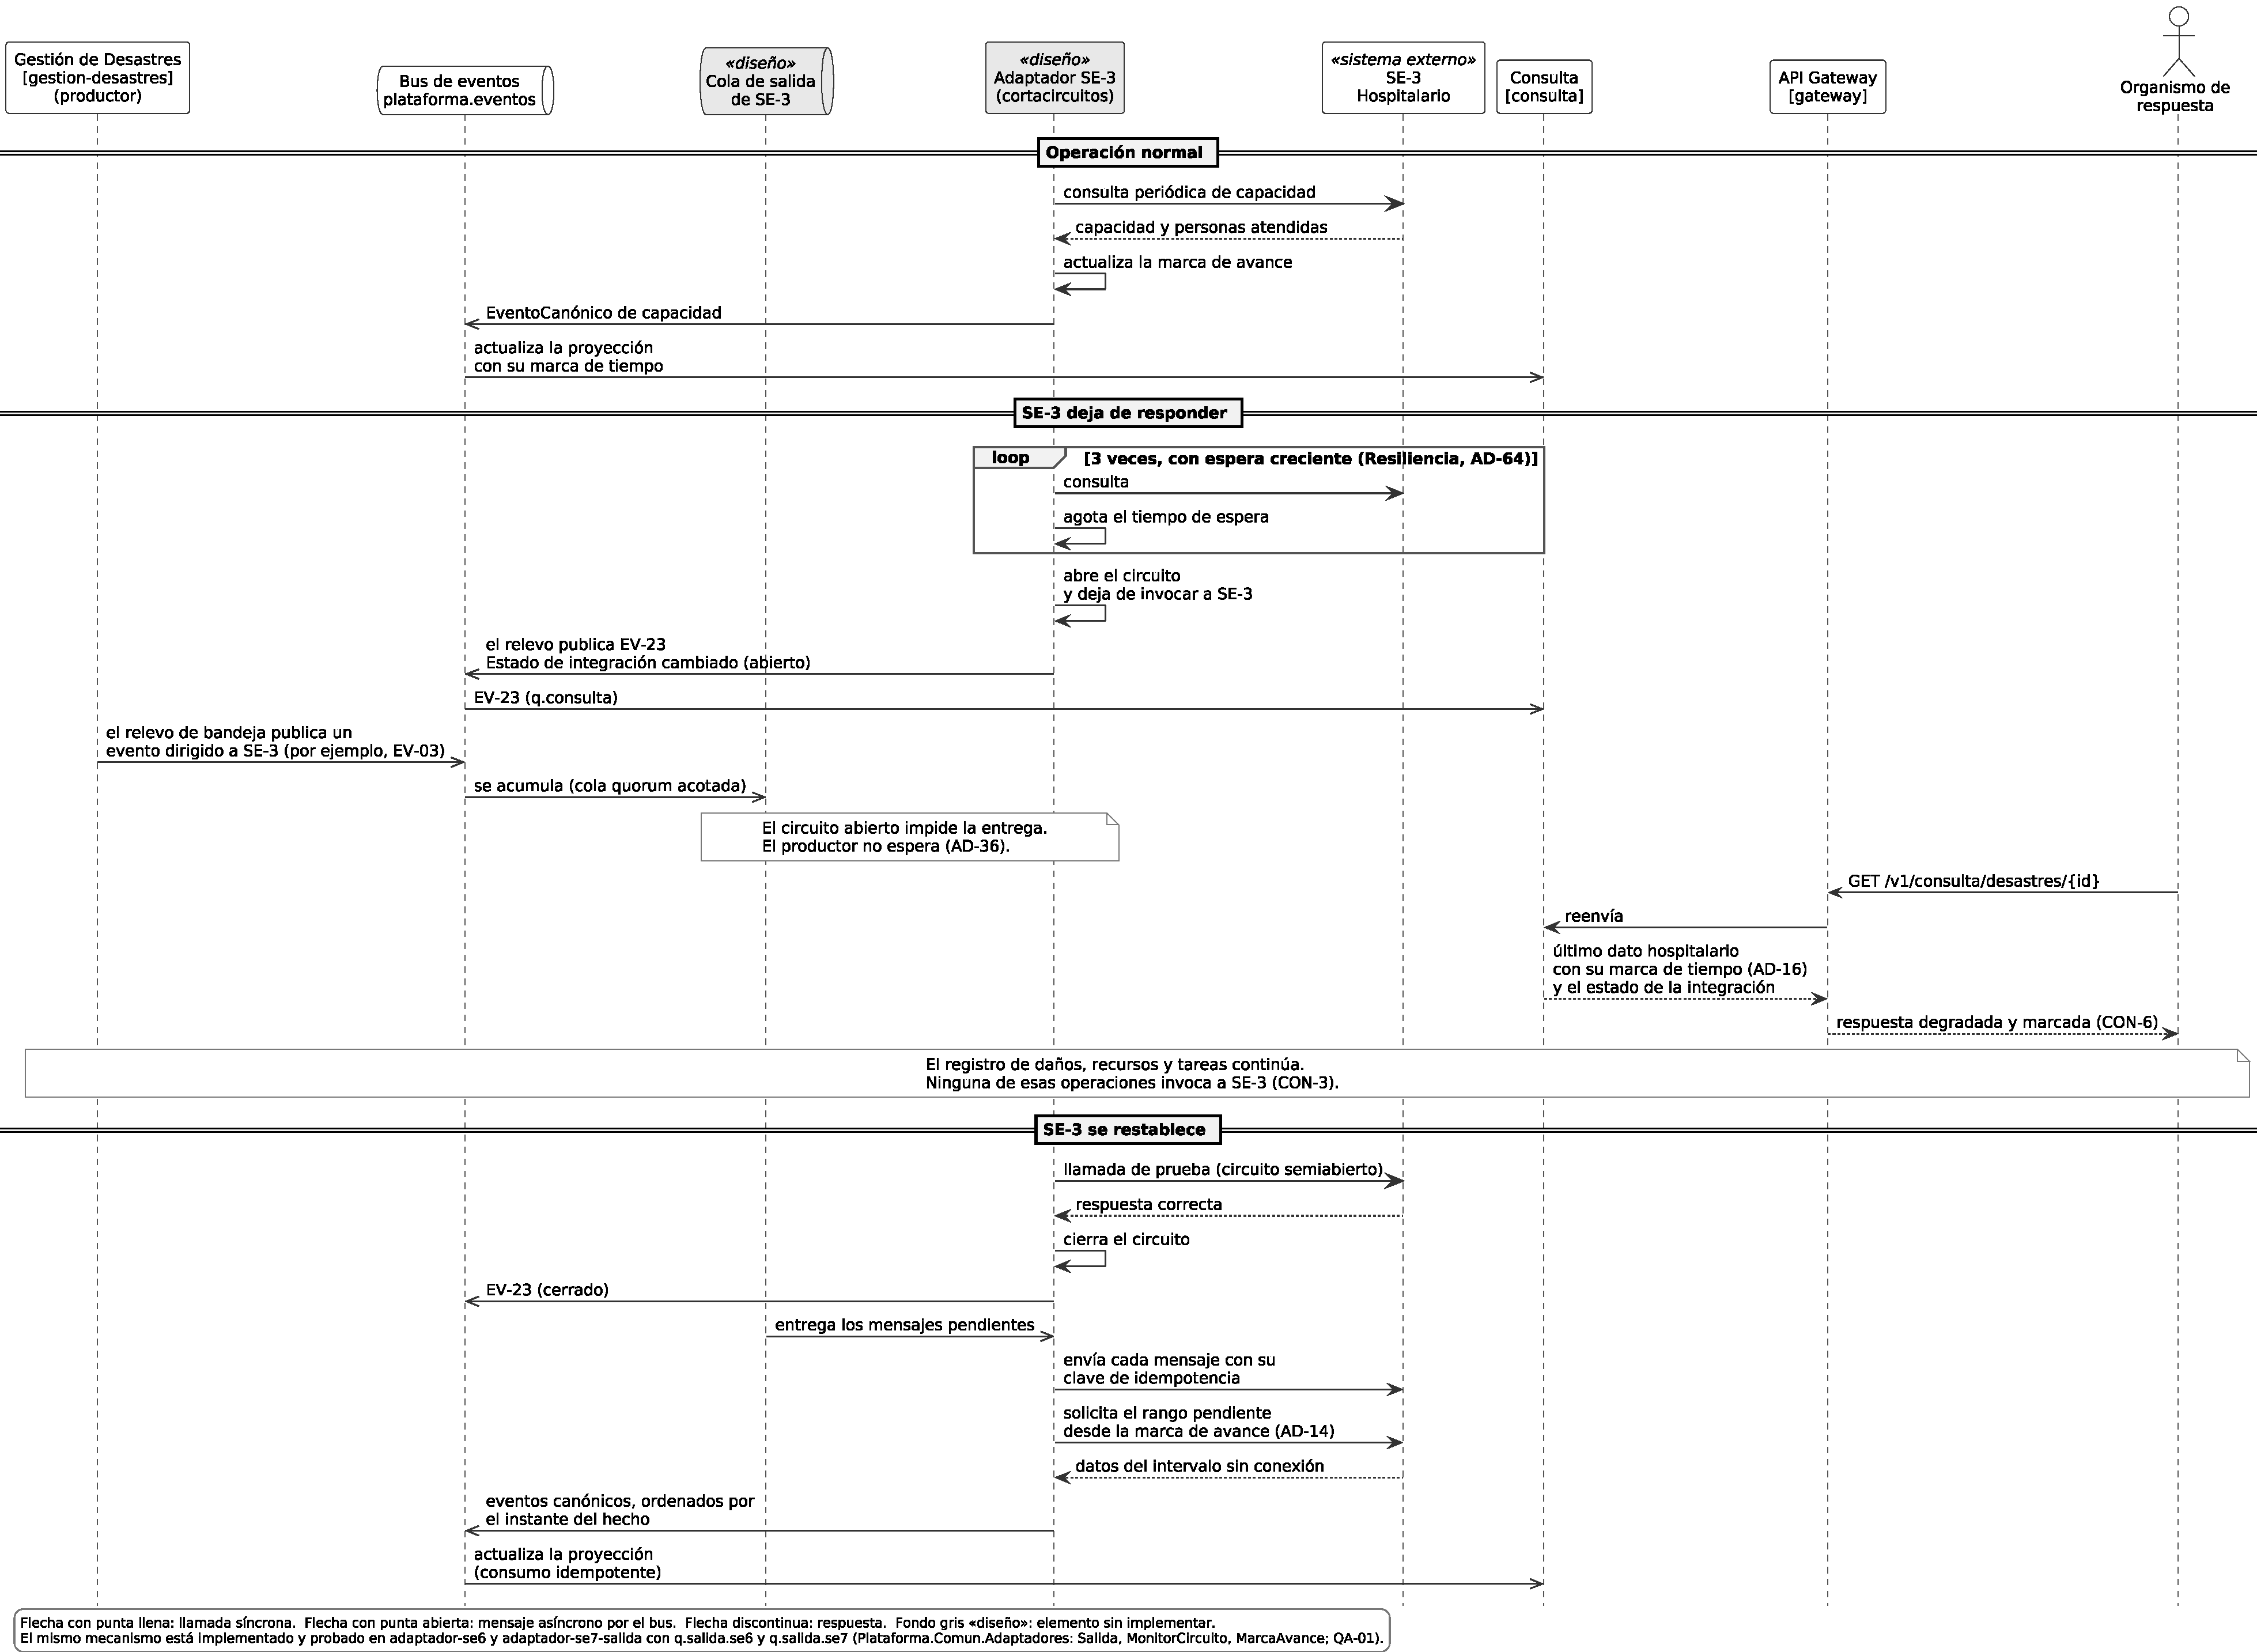
\includegraphics[width=\linewidth,height=0.86\textheight,keepaspectratio]{figuras/seq_eo3}
\caption{Diagrama de secuencia de CU-2: fallo de SE-3 con cortacircuitos, cola de salida y marca de
avance (EO-3).}
\label{fig:seq-eo3}
\end{figure}
\end{landscape}

\subsubsection{Caso de uso CU-3: evaluación de daños sin conexión (EO-4)}

\begin{longtable}{L{3.2cm} L{12.6cm}}
\cabecera{2}{tab:cu3}{Especificación del caso de uso CU-3}{\textbf{Campo} & \textbf{Contenido}}
Nombre & Registrar evaluaciones de daño sin conexión y sincronizarlas \\
Casos de uso primarios & FP-06 \\
Actores & Evaluador de campo (primario), operador de la plataforma \\
Disparador & El evaluador registra una evaluación en una zona sin conectividad \\
Precondiciones & El evaluador descargó previamente los catálogos, los desastres y los activos con
su versión (\texttt{GET /\br{}v1/\br{}descarga}) \\
Flujo principal &
1. El evaluador registra la evaluación y captura las evidencias.\newline
2. El cliente móvil, en una transacción local, guarda la evaluación en la réplica local y encola
una operación con una copia completa del contenido y la versión base del activo (AD-44).\newline
3. Al recuperar la conexión, el cliente envía el lote de operaciones con el instante de envío del
dispositivo y con los metadatos y el hash de cada evidencia.\newline
4. Evaluación de Daños registra el desfase del reloj del dispositivo (S-5) y procesa cada operación
en su propia transacción.\newline
5. Operación sin conflicto: inserta la versión de la evaluación, aumenta la versión del activo y
escribe EV-09 en la bandeja de salida (AD-45).\newline
6. El microservicio responde el resultado de cada operación. El cliente retira de la cola solo las
operaciones que tienen respuesta.\newline
7. El cliente sube cada evidencia (\texttt{PUT /v1/evidencias/\{id\}}). El microservicio verifica
el hash declarado.\newline
8. El publicador lee la bandeja de salida y publica los eventos. Consulta de Daños actualiza sus
proyecciones y Auditoría registra los eventos \\
Flujos alternativos &
5a. Conflicto: el activo tiene una versión mayor que la versión base, producida por otro
dispositivo (AD-43). El microservicio guarda la evaluación entrante con estado \enquote{en
conflicto}, conserva la versión vigente, registra el conflicto y escribe EV-10 en la bandeja de
salida. Un usuario autorizado decide después qué versión prevalece. Ninguna versión se elimina
(AD-32).\newline
5b. Reenvío: el identificador de la operación ya se procesó. El microservicio devuelve el resultado
guardado y no crea registros (AD-44).\newline
5c. Posible duplicado: existe otra evaluación del mismo activo dentro de la ventana configurada. Se
marca para revisión (AD-33).\newline
5d. Operación inválida: falta un atributo obligatorio o el tipo no existe. Se responde el motivo y
la evaluación no se guarda.\newline
6a. La conexión se interrumpe antes de la respuesta: las operaciones permanecen en la cola y se
reenvían \\
Postcondiciones & 0 evaluaciones perdidas, 0 sobrescrituras silenciosas y 0 duplicados. Cada
conflicto está en la bandeja de revisión con ambas versiones \\
Escenarios de calidad & QA-14 \\
Decisiones & AD-29 a AD-33, AD-43, AD-44, AD-45 \\
\end{longtable}

La carga de sincronización no afecta la coordinación, porque el camino de escritura de evaluaciones
está separado del camino de consulta y las proyecciones se actualizan de forma asíncrona (AD-34).
La \cref{fig:seq-eo4} muestra la secuencia con un conflicto.

\begin{figure}[p]
\centering
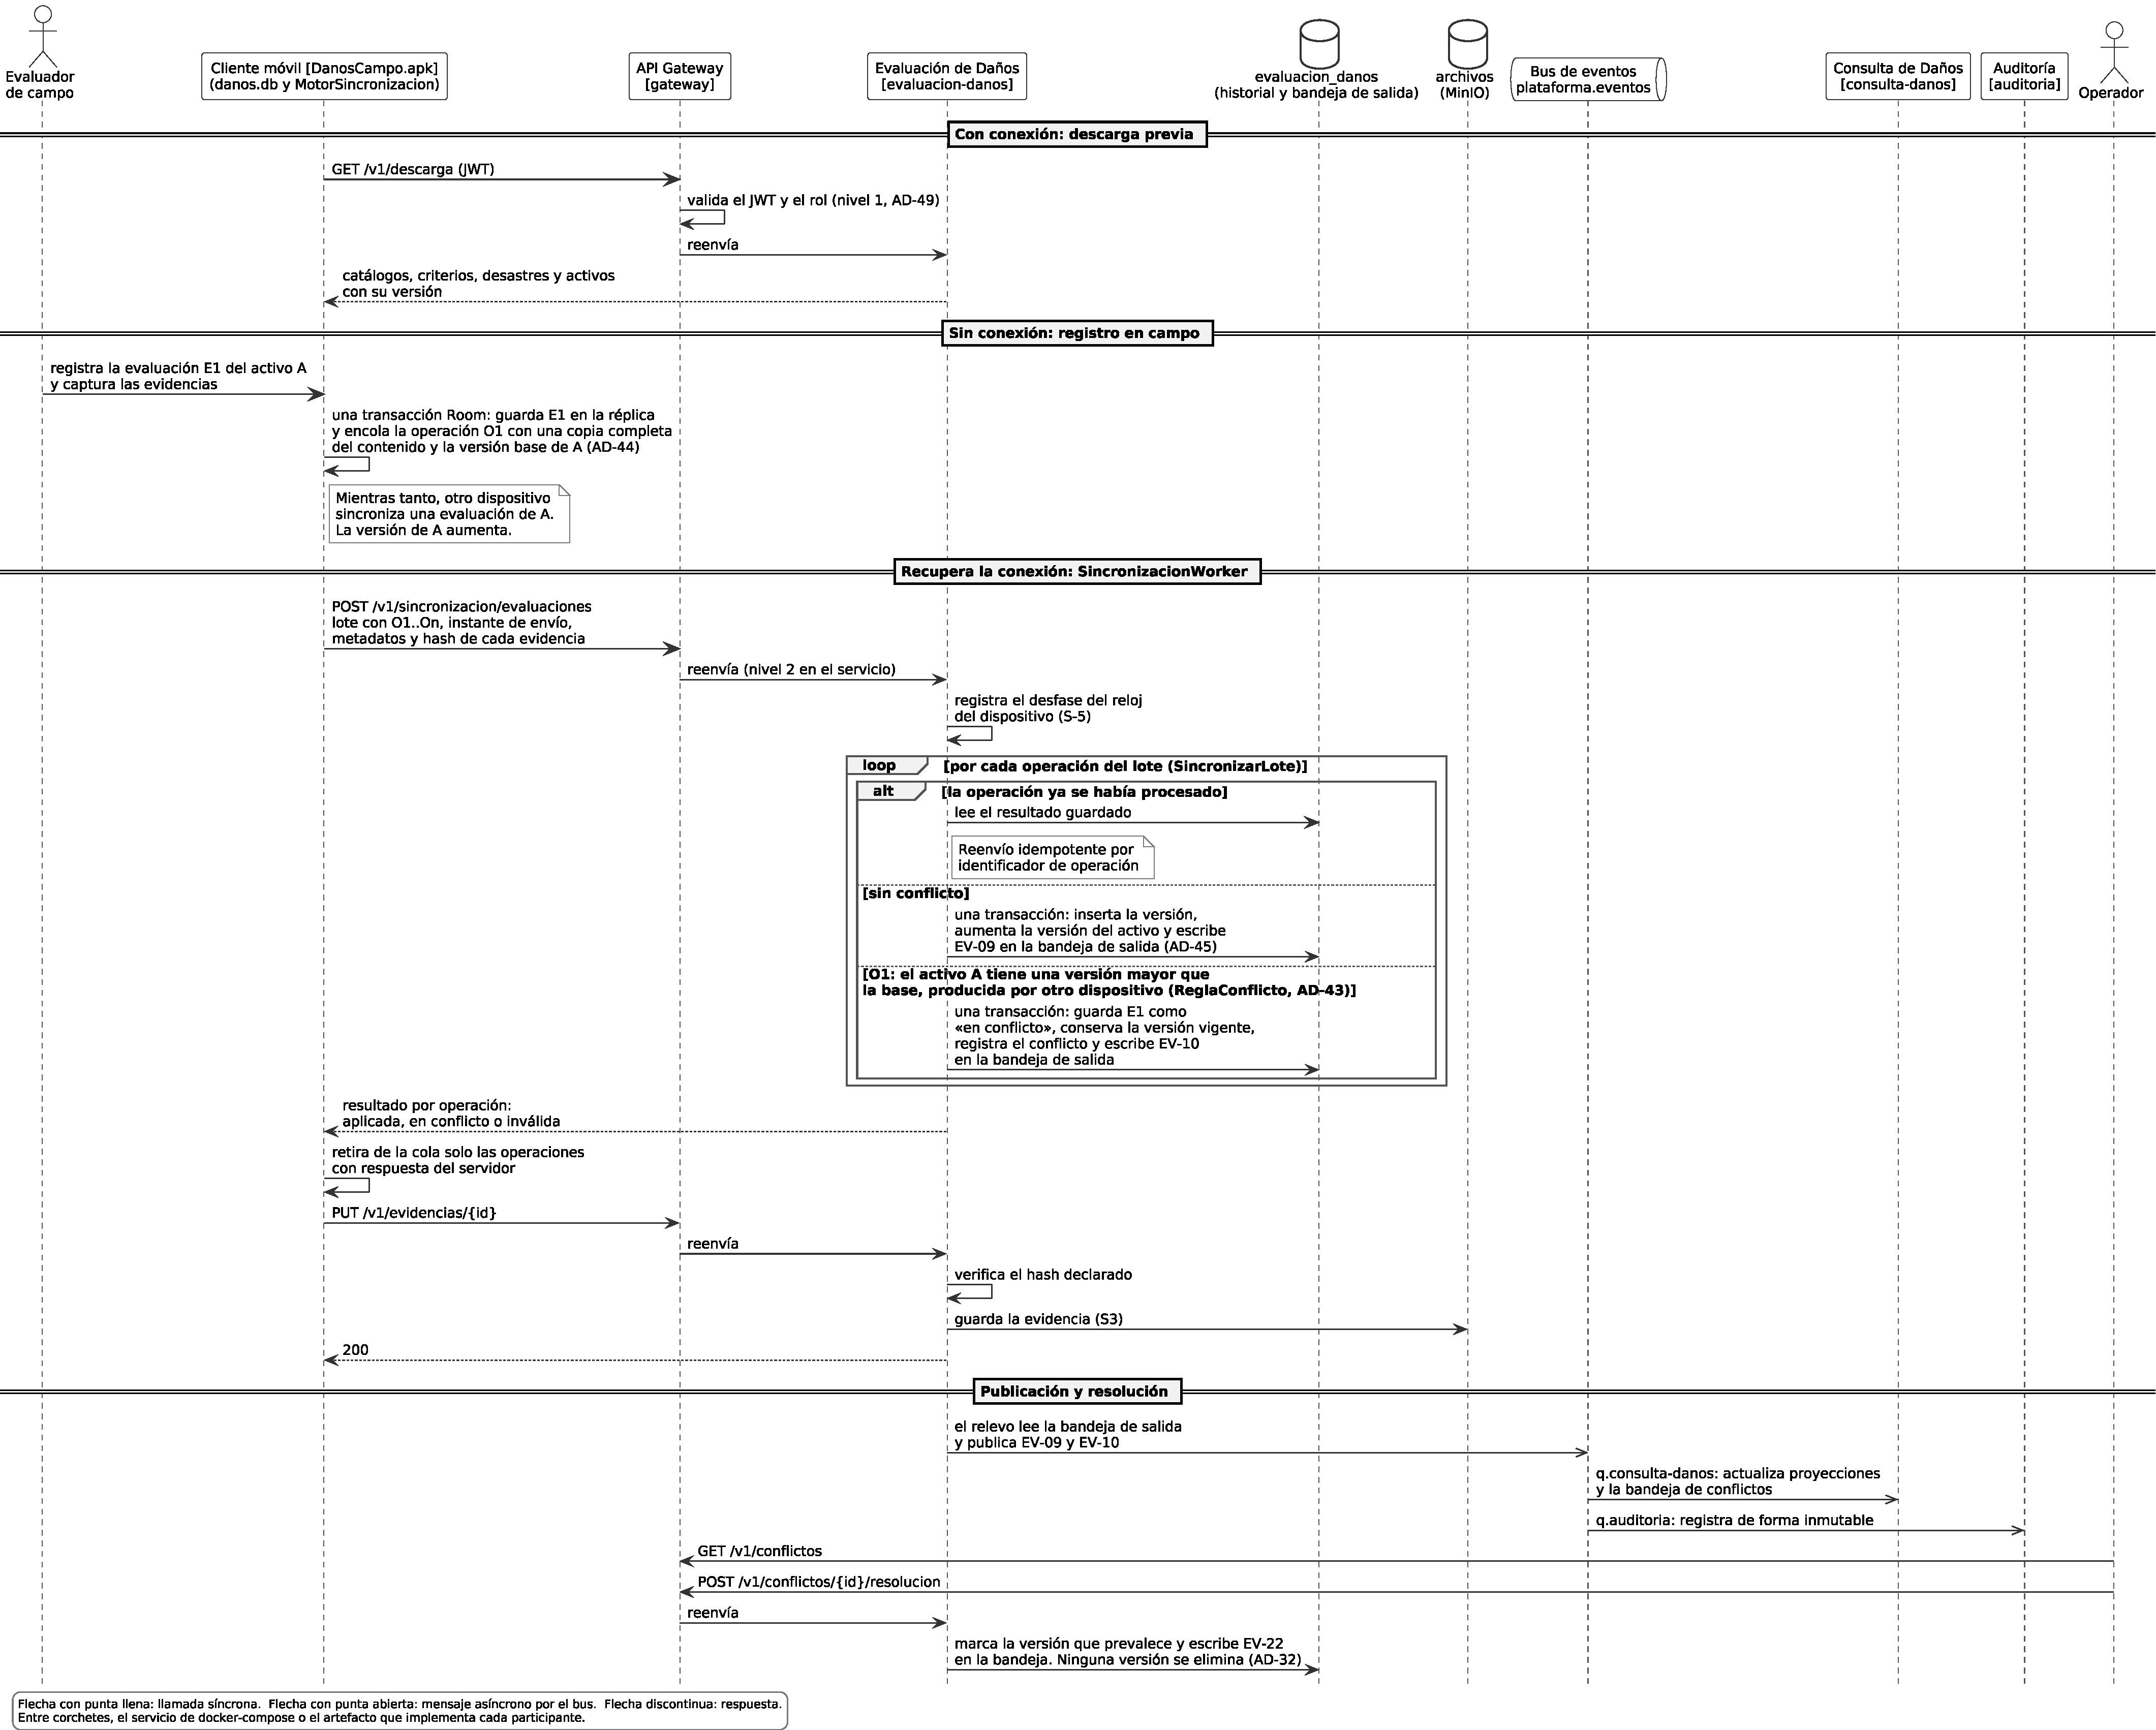
\includegraphics[width=\linewidth,height=0.9\textheight,keepaspectratio]{figuras/seq_eo4}
\caption{Diagrama de secuencia de CU-3: sincronización sin conexión con un conflicto (EO-4).}
\label{fig:seq-eo4}
\end{figure}
\clearpage

\subsubsection{Caso de uso CU-4: registro del desastre en campo}
\label{sec:cu4}

CU-4 se agrega en la versión 1.2 y permite registrar desde el cliente móvil el desastre al que se
asocian las evaluaciones (E-42, AD-48). Pertenece a Gestión de Desastres y complementa el mínimo a) de
la entrega 2, que realiza CU-3. Aparece en la \cref{fig:casos-uso} como el caso
\enquote{Registrar y caracterizar un desastre en campo} (RF-GD-02), con el actor organismo de
respuesta en campo.

\begin{longtable}{L{3.2cm} L{12.6cm}}
\cabecera{2}{tab:cu4}{Especificación del caso de uso CU-4}{\textbf{Campo} & \textbf{Contenido}}
Nombre & Registrar un desastre en campo desde el cliente móvil, con o sin conexión \\
Requisitos & RF-GD-02, RF-GD-03, RF-GD-05, RF-GD-08 \\
Actores & Organismo de respuesta o autoridad en campo (primario), Proveedor de identidad \\
Disparador & El usuario observa un fenómeno que no está registrado en la plataforma \\
Precondiciones & El usuario inició sesión con OpenID Connect y PKCE y tiene el rol
\texttt{organismo} o \texttt{autoridad} (AD-49). El cliente tiene el catálogo de tipos descargado
o usa los tipos de RN-1 \\
Flujo principal &
1. El usuario abre la pantalla Registrar desastre (paquete \texttt{presentacion/\br{}desastre}) e
ingresa el tipo, el nombre, la descripción, la severidad, el responsable, el instante de inicio, la
ubicación y el radio de la zona.\newline
2. El dominio del cliente (\texttt{RegistroDesastre}) valida los atributos mínimos y los códigos
DIVIPOLA de los municipios.\newline
3. El cliente genera el identificador del desastre y guarda el registro con estado pendiente en la
tabla \texttt{registro\_\br{}desastre} de \texttt{danos.db}, en una transacción local (AD-44).\newline
4. Con conexión, \texttt{SincronizacionWorker} invoca a \texttt{EnviadorDesastres}, que envía
\texttt{POST /\br{}v1/\br{}desastres} con el identificador y el token por el \texttt{gateway}.\newline
5. El \texttt{gateway} valida el token y el rol (nivel 1). \texttt{gestion-\br{}desastres} valida el
token de nuevo (nivel 2), valida el tipo contra el catálogo y crea el desastre con el
identificador recibido.\newline
6. En la misma transacción, \texttt{gestion-\br{}desastres} escribe EV-03 en su bandeja de salida. El
relevo lo publica en \texttt{plataforma.\br{}eventos} (AD-45).\newline
7. El servicio responde 201. El cliente marca el registro como enviado.\newline
8. \texttt{consulta}, \texttt{evaluacion-\br{}danos}, \texttt{reconstruccion} y \texttt{auditoria}
consumen EV-03 desde sus colas. El desastre aparece en el mapa de la consola \\
Flujos alternativos &
4a. Sin red, error 5xx o token vencido (401): el registro permanece pendiente y se reintenta. Un
401 pide al usuario iniciar sesión de nuevo. Ningún registro se pierde.\newline
5a. Reenvío del mismo identificador por el mismo autor: el servicio devuelve el desastre ya
registrado y no crea otro (idempotencia, AD-48).\newline
5b. El identificador pertenece a otro autor: el servicio responde 409 \texttt{ID\_EXISTE}.\newline
5c. Error de validación o de permiso (4xx): el registro queda rechazado con el motivo del servidor
y el cliente no insiste \\
Postcondiciones & El desastre existe una sola vez, en estado Registrado, con su autor y su
organización. EV-03 está en el registro de auditoría \\
Escenarios de calidad & QA-07, QA-11, QA-14 \\
Decisiones & AD-06, AD-07, AD-22, AD-44, AD-45, AD-48, AD-49 \\
\end{longtable}

La \cref{fig:seq-registro-desastre} muestra la secuencia con un envío fallido y su reenvío
idempotente. Las líneas de vida usan los nombres del código.

\begin{figure}[p]
\centering
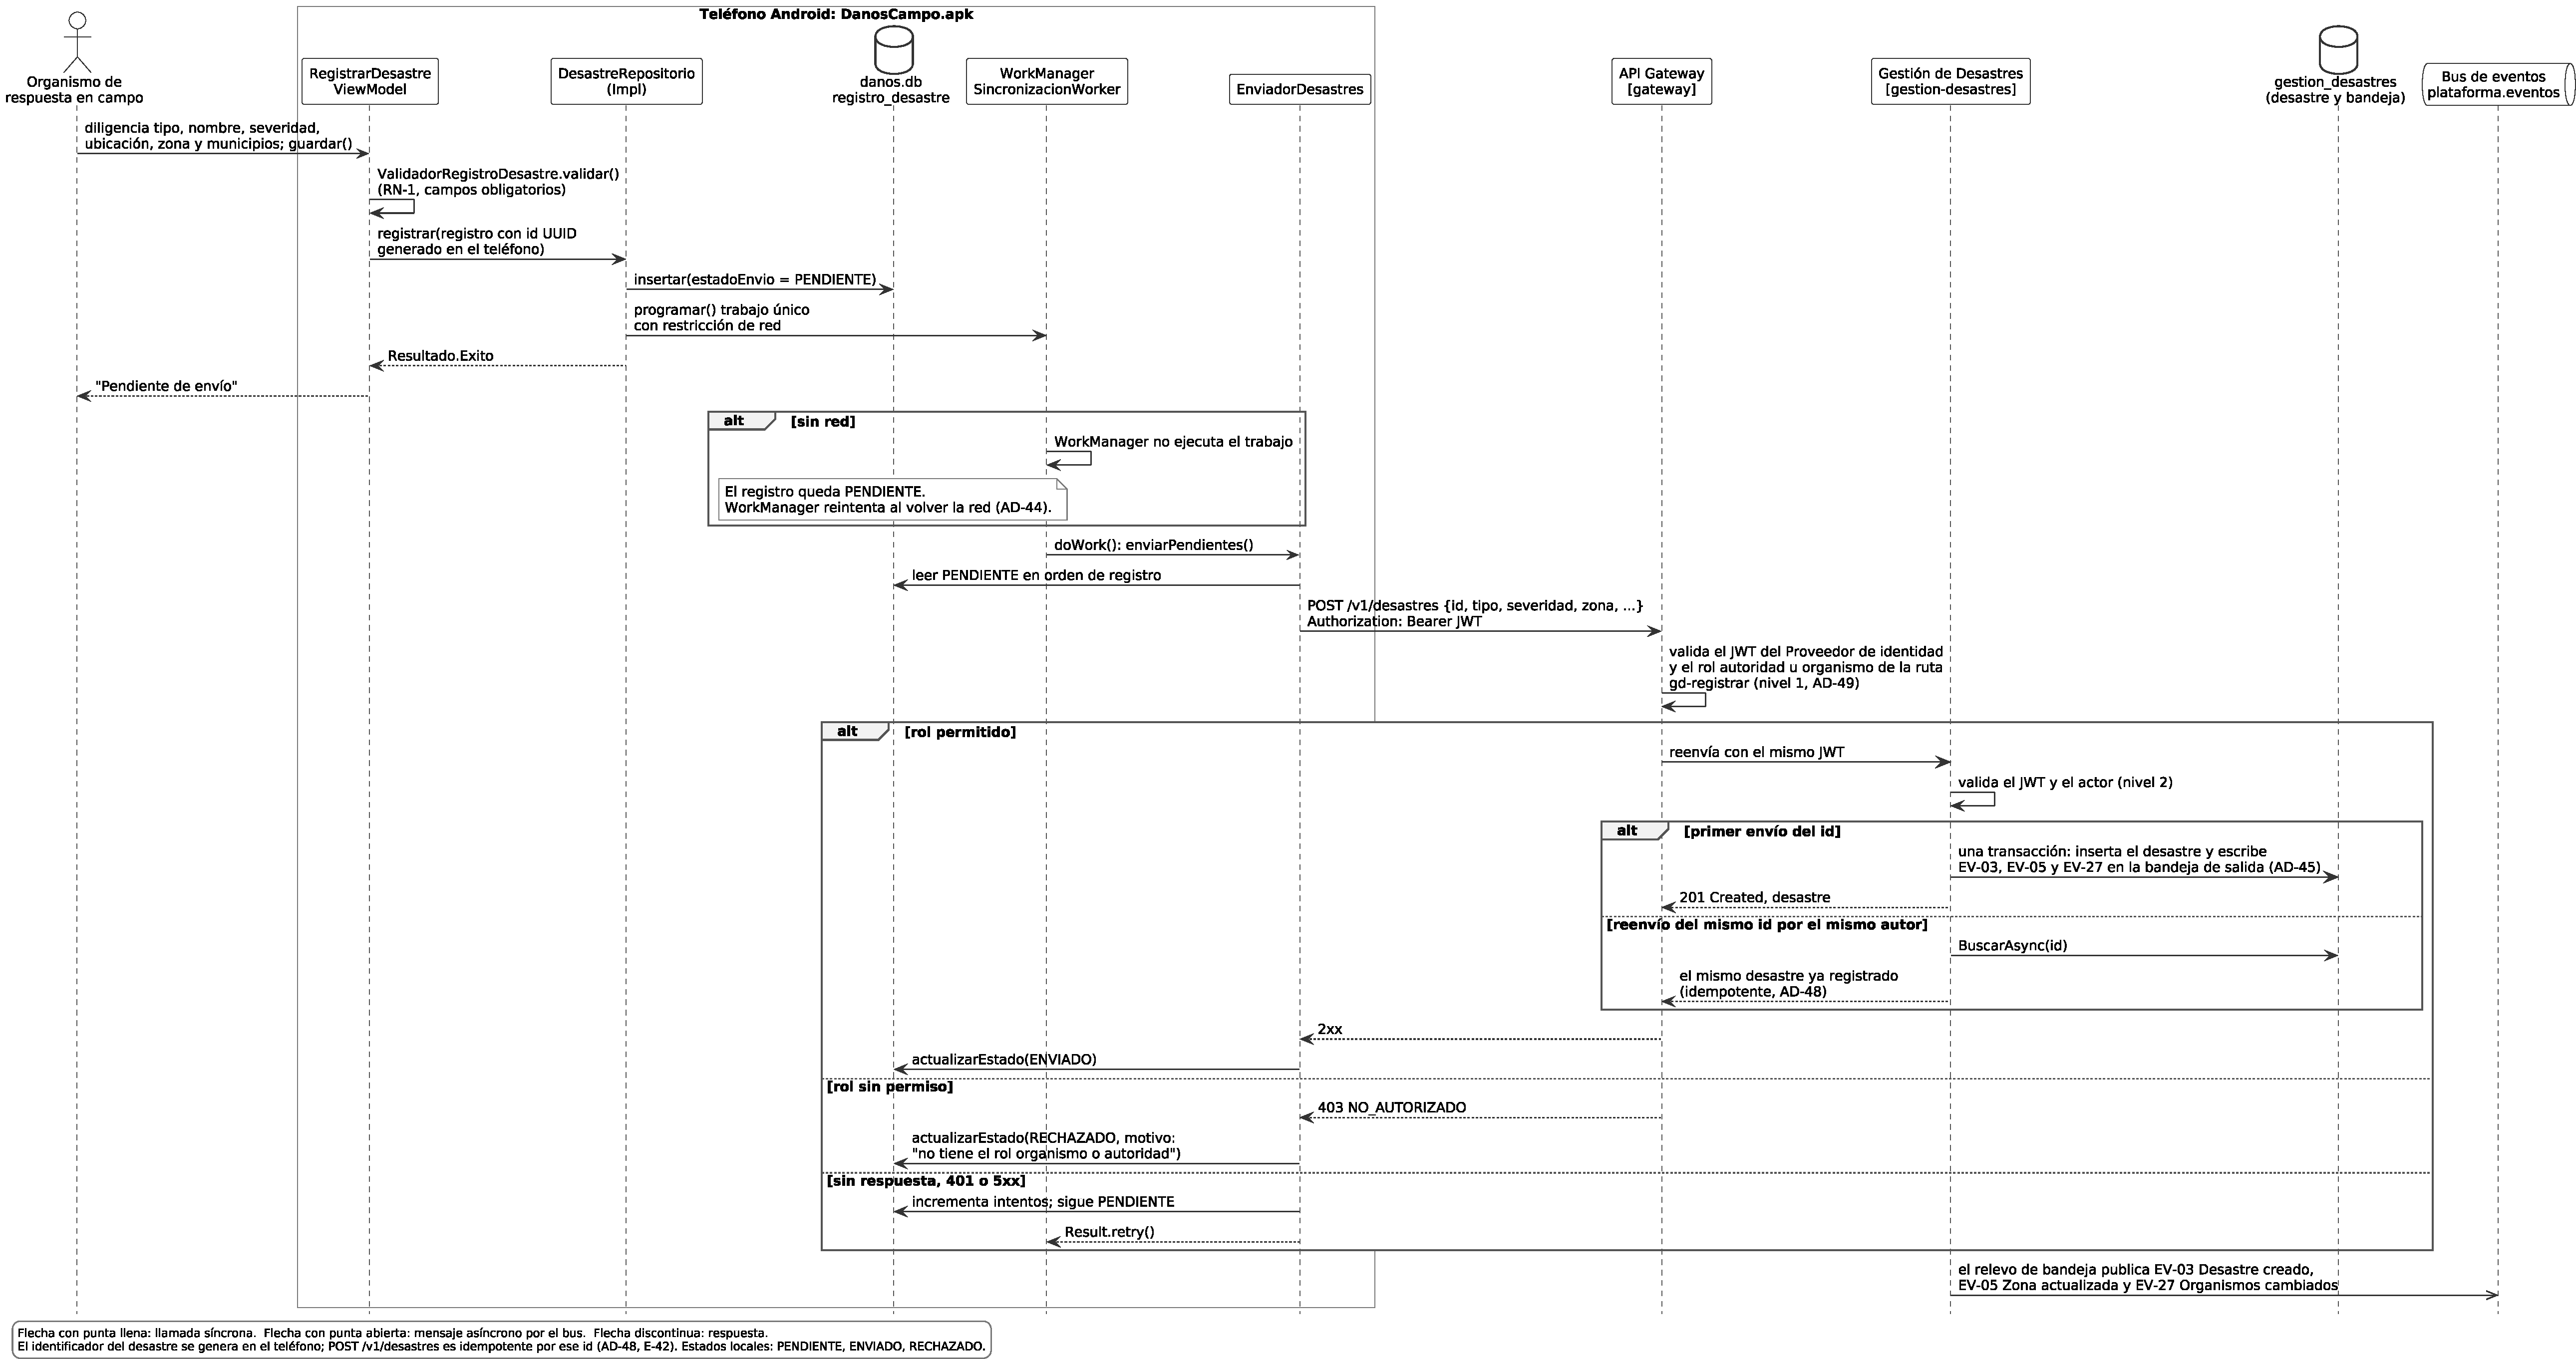
\includegraphics[width=\linewidth,height=0.9\textheight,keepaspectratio]{figuras/seq_registro_desastre}
\caption{Diagrama de secuencia de CU-4: registro del desastre en campo con reenvío idempotente
(AD-48).}
\label{fig:seq-registro-desastre}
\end{figure}
\clearpage

\subsubsection{Caso de uso CU-5: crear y dar seguimiento a proyectos de reconstrucción (EO-5)}
\label{sec:cu5}

CU-5 realiza el mínimo b) de la entrega 2. Resume los casos de uso CU-01 a CU-06 del documento de
diseño del módulo de Reconstrucción \cite{diseno-rc}, donde están sus diagramas de secuencia.

\begin{longtable}{L{3.2cm} L{12.6cm}}
\cabecera{2}{tab:cu5}{Especificación del caso de uso CU-5}{\textbf{Campo} & \textbf{Contenido}}
Nombre & Crear proyectos por lote a partir de evaluaciones validadas, aprobarlos con jurisdicción y
registrar su avance y su costo \\
Casos de uso primarios & FP-08. Requisitos RF-RC-01, RF-RC-03, RF-RC-04, RF-RC-05, RF-RC-07 y
RF-RC-08 \\
Actores & Autoridad (primario), responsable de proyecto, auditor, SE-6, SE-7 \\
Disparador & Un desastre está en reconstrucción y la autoridad decide intervenir activos con daño grave
o destrucción total \\
Precondiciones & El usuario inició sesión y tiene el rol \texttt{autoridad} (AD-49). El desastre está
en estado En reconstrucción. Las evaluaciones validadas están en la copia local de Reconstrucción
(AD-46) \\
Flujo principal &
1. La autoridad consulta las candidatas de su jurisdicción (\texttt{GET /\br{}v1/\br{}reconstruccion/\br{}candidatas}).\newline
2. Envía el desastre, las evaluaciones y la clave de idempotencia
(\texttt{POST /\br{}v1/\br{}proyectos:lote}).\newline
3. \texttt{reconstruccion} valida la jurisdicción y el lote, y crea un proyecto por activo en estado
Formulado. En una transacción guarda los proyectos, su historial y un EV-18 por proyecto en la bandeja
de salida (AD-40, AD-41, AD-45).\newline
4. El relevo publica EV-18. Los adaptadores entregan el proyecto a SE-7 y a SE-6 por sus colas de salida
(AD-36, AD-37).\newline
5. La autoridad asigna presupuesto, fuente y cronograma, y asigna el responsable, con justificación.
Reconstrucción publica EV-19 para el presupuesto y la fuente, y EV-20 para el cronograma y el
responsable (E-10).\newline
6. La autoridad con jurisdicción sobre el territorio del proyecto lo aprueba: local si es municipal,
regional si abarca varios municipios de un departamento y nacional si abarca varios departamentos
(E-20). Reconstrucción publica EV-20.\newline
7. El responsable registra el contratista, o se usa el que reportó SE-7 (EV-24), e inicia la
ejecución. Reconstrucción publica EV-20.\newline
8. El responsable registra avance y costo (\texttt{POST /\br{}v1/\br{}proyectos/\{id\}/\br{}avance}).
Reconstrucción actualiza los acumulados, guarda el historial y publica EV-20, que llega a SE-6 y a
SE-7.\newline
9. Consulta del Programa actualiza el consolidado y Auditoría registra los eventos \\
Flujos alternativos &
3a. Un lote con alguna evaluación fuera de la jurisdicción se rechaza entero con 403.\newline
3b. Una evaluación incumple una regla: no se crea ningún proyecto y se informa cuáles fallaron (422).\newline
3c. Reenvío con la misma clave de idempotencia: se devuelven los mismos proyectos.\newline
6a. Quien no ve el proyecto recibe 404. Quien lo ve y no es la autoridad que lo aprueba recibe 403
(E-39).\newline
6b. Faltan presupuesto, fuente, responsable o cronograma: 422.\newline
8a. El proyecto no está en ejecución: 409. Un valor fuera de rango: 422.\newline
8b. El costo ejecutado supera el presupuesto: el proyecto queda marcado en sobrecosto y el registro se
acepta.\newline
4a, 8c. SE-6 o SE-7 no responden: la operación se confirma y la entrega queda en su cola de salida \\
Postcondiciones & Cada proyecto conserva el vínculo con su evaluación de origen. Cada cambio queda en
el historial de solo inserción, con valor anterior, valor nuevo, autor y justificación, y el auditor
puede consultarlo \\
Escenarios de calidad & QA-15, QA-13, QA-01 \\
Decisiones & AD-36, AD-37, AD-40, AD-41, AD-42, AD-45, AD-46, AD-47 \\
\end{longtable}

\subsection{Estado consolidado de los drivers}

El \cref{tab:estado-drivers} indica, para cada caso de uso primario y cada atributo de calidad, la
iteración de ADD en la que se atendió y el mecanismo que lo resuelve. Los mecanismos aparecen en
las vistas anteriores (\cref{tab:decisiones-vistas}).

\begin{longtable}{L{5.2cm} L{1.9cm} L{8.7cm}}
\cabecera{3}{tab:estado-drivers}{Estado consolidado de los diez casos de uso primarios y de los diez
atributos de calidad}{\textbf{Driver} & \textbf{Iteración} & \textbf{Mecanismo principal}}
FP-01. Registrar un desastre desde un sistema externo & 2 & Microservicio de Gestión de Desastres y
catálogo de tipos \\
FP-02. Consultar y monitorear el estado del desastre & 4 & Microservicio de Consulta con modelo de
lectura separado \\
FP-03. Actualizar severidad y delimitación & 2 y 5 & Validación contra el catálogo e historial
versionado \\
FP-04. Consolidar reportes de distintas fuentes & 3 & Correlación híbrida y procedencia \\
FP-05. Notificar a los organismos & 3 & Microservicio de Notificación con suscripciones \\
FP-06. Registrar una evaluación de daños y sincronizarla & 7 y 8 & Catálogos configurables, réplica
local, cola de operaciones, regla determinista de conflicto y bandeja de salida \\
FP-07. Solicitar y asignar un recurso & 9 y 10 & Catálogo con dos vías de escritura y reserva
optimista con confirmación asíncrona \\
FP-08. Crear proyectos de reconstrucción & 11 & Disparador por transición de estado y creación por
lote \\
FP-09. Asignar responsabilidades y dar seguimiento a las tareas & 5 & Autorización en dos niveles
con la regla del organismo responsable, y auditoría centralizada \\
FP-10. Registrar personas afectadas con protección de datos & 5 & Cifrado por columna y control de
acceso por organización \\
\midrule
Disponibilidad & 1 y 6 & Microservicios con réplicas activas y despliegue en dos regiones \\
Interoperabilidad & 3 y 9 & Contrato de adaptador y evento canónico \\
Escalabilidad & 4 & Separación del modelo de lectura y del modelo de escritura \\
Resiliencia & 1, 3, 9 y 10 & Cortacircuitos por adaptador con tiempo de espera y reintento,
degradación controlada y colas de salida acotadas \\
Recuperación ante fallos & 6 & Réplica activa local, réplica en espera regional, conmutación
automática y resincronización de estado \\
Seguridad & 5 y 7 & Autenticación en el API Gateway, autorización en dos niveles y cifrado por
columna \\
Trazabilidad & 5, 9 y 11 & Microservicio de Auditoría alimentado por el bus, procedencia de cada
dato e historial de solo inserción \\
Rendimiento & 4 y 8 & Caché de geometrías y proyecciones precalculadas \\
Modificabilidad & 2, 3 y 7 & Catálogos de tipos y categorías configurables, y contrato de
adaptador \\
Integridad de datos & 8 & Detección determinista de conflictos sin resolución automática, cola de
operaciones idempotente y escalamiento a un usuario autorizado \\
\end{longtable}

\subsection{Representación de las decisiones en las vistas}
\label{sec:decisiones-vistas}

El \cref{tab:decisiones-vistas} indica en qué vista y en qué elemento se representa cada decisión
del \cref{tab:decisiones} y de la \cref{sec:tecnologia}. Las abreviaturas son: L, vista lógica
(\cref{fig:vista-logica}); P, vista de procesos (\cref{fig:vista-procesos}); F, vista física de
diseño (\cref{fig:vista-despliegue}); FI, vista física de la implementación
(\cref{fig:vista-despliegue-impl}); I, vista de implementación
(\cref{fig:vista-implementacion,fig:vista-implementacion-movil}); CU, vista de casos de uso
(\cref{fig:seq-eo1,fig:seq-eo3,fig:seq-eo4,fig:seq-registro-desastre}); INT, modelo de integración
(\cref{fig:integracion}).

\begin{longtable}{L{1.3cm} L{5.2cm} L{1.6cm} L{7.4cm}}
\cabecera{4}{tab:decisiones-vistas}{Vista y elemento en que se representa cada decisión}{\textbf{ID} &
\textbf{Decisión} & \textbf{Vista} & \textbf{Elemento}}
AD-01 & Microservicios con almacén propio & L, F, FI, I & Componentes \enquote{microservicio}, cada
uno con su almacén. Artefactos \texttt{gestion-\br{}desastres}, \texttt{evaluacion-\br{}danos},
\texttt{reconstruccion}, \texttt{consulta-\br{}programa}, \texttt{consulta}, \texttt{consulta-\br{}danos} y
\texttt{auditoria}, cada uno con su base en \texttt{db}. Proyectos \texttt{*.Api},
\texttt{*.Aplicacion}, \texttt{*.Dominio} e \texttt{*.\br{}Infraestructura} \\
AD-02 & Bus de eventos & L, P, F, FI & Bus de eventos con colas \texttt{q.*} por consumidor. Nodo de
mensajería. Artefactos \texttt{bus1} a \texttt{bus3} \\
AD-03 & Un adaptador por sistema externo & L, P, FI, I, INT & Componentes Adaptador de SE-n.
Implementados: \texttt{adaptador-se2}, \texttt{adaptador-se6}, \texttt{adaptador-\br{}se7-\br{}salida} y
\texttt{adaptador-\br{}se7-\br{}entrada}, proyectos \texttt{AdaptadorSe2}, \texttt{AdaptadorSe6} y
\texttt{AdaptadorSe7}. Los demás con estereotipo «diseño» \\
AD-04 & API Gateway & L, P, F, FI & Componente API Gateway. Nodo de entrada. Artefacto
\texttt{gateway} ×2 con \texttt{rutas.json}. Proyecto \texttt{Plataforma.\br{}Gateway} \\
AD-05 & Cortacircuitos, tiempo de espera y reintento & P, INT, CU & Proceso Adaptador SE-n.
Componentes Cortacircuitos y Cliente del sistema externo. Secuencia de CU-2 \\
AD-06 & Registro y actualización en un microservicio & L & Componente Gestión de Desastres \\
AD-07 & Catálogo de tipos y ciclo de vida & L, CU & Componente Gestión de Desastres. Paso 3 de
CU-1 \\
AD-08 & Cuatro capas & L, I & Paquetes de capa. Capas internas del microservicio tipo y del cliente
móvil \\
AD-09 & Contrato de adaptador y evento canónico & L, I, INT & Interfaz \texttt{ContratoAdaptador} y
esquema \texttt{EventoCanónico}. En el código, \texttt{IContratoAdaptador} de
\texttt{Plataforma.\br{}Comun.\br{}Adaptadores} y \texttt{Sobre} con los esquemas
\texttt{EV-nn.v1.json} de \texttt{Plataforma.\br{}Comun.\br{}Eventos} \\
AD-10 & Correlación híbrida & L, CU & Componente Consolidación. Paso 2 de CU-1 \\
AD-11 & Procedencia de cada dato & L, CU & Componente Consolidación. EV-02 en CU-1 \\
AD-12 & Consolidación separada & L, P & Componente y proceso Consolidación, con su cola \\
AD-13 & Notificación con suscripciones & L, CU & Componente Notificación. Paso 4 de CU-1 \\
AD-14 & Marca de avance & P, INT, CU & Proceso Adaptador SE-n. Almacén Marca de avance. Paso 7 de
CU-2 \\
AD-15 & Modelo de lectura separado & L, P, F & Microservicios de consulta y sus proyecciones. Nodo
de cómputo de consulta \\
AD-16 & Marca de tiempo del dato & P, CU & Nota de degradación controlada. Paso 3 de CU-2 \\
AD-17 & Caché de geometrías & L, F, FI & Almacén Caché de geometrías [\texttt{cache}]. Artefacto
\texttt{cache} (Redis) \\
AD-18 & Más réplicas de consulta & P, F & Multiplicidad [2..N] de los procesos y de los nodos de
consulta \\
AD-19 & Priorización y degradación en el API Gateway & L, P & Componente y proceso API Gateway, con
su nota \\
AD-20 & Historial versionado & L, I & Almacenes de Gestión de Desastres y de Evaluación de Daños.
Paquete \texttt{Persistencia} de \texttt{GestionDesastres.\br{}Infraestructura} y de
\texttt{EvaluacionDanos.\br{}Infraestructura} \\
AD-21 & Auditoría centralizada & L, P, CU & Componente Auditoría y registro de auditoría. Cola de
auditoría \\
AD-22 & Autorización en dos niveles & L, I, CU & API Gateway con la metadata \texttt{roles} y
\texttt{reglaDominio} de \texttt{rutas.json} (nivel 1). \texttt{Plataforma.\br{}Comun.\br{}Seguridad} y las
reglas de dominio de cada \texttt{*.Api} (nivel 2). Paso 5 de CU-4 \\
AD-23 & Cifrado por columna & L & Almacén de Personas Afectadas \\
AD-24 & Réplica activa con sondeo de salud & P, F & Multiplicidad de los procesos y de los
artefactos \\
AD-25 & Ejecución híbrida & P, F & Procesos persistentes y adaptador efímero. Nodo de ejecución bajo
demanda \\
AD-26 & Dos regiones con conmutación & F & Región primaria, región secundaria, enrutador global y
replicación asíncrona \\
AD-27 & Resincronización de estado & F & Ruta de replicación entre los nodos de datos \\
AD-28 & Catálogo de tipos de activo & L, I & Componente Evaluación de Daños. Clase
\texttt{CatalogoTipos} de \texttt{EvaluacionDanos.\br{}Dominio} \\
AD-29 & Registro preliminar & CU & Atributo de estado de la evaluación en CU-3 \\
AD-30 & Historial versionado de evaluaciones & L, CU & Almacén de Evaluación de Daños. Paso 5 de
CU-3 \\
AD-31 & Réplica local en el cliente móvil & L, F, FI, I & Componente Cliente móvil. Artefacto
\texttt{danos.db} en el teléfono. Paquete \texttt{infraestructura/\br{}local} \\
AD-32 & Detección sin resolución automática & L, CU & Componente Evaluación de Daños. Flujo 5a de
CU-3 \\
AD-33 & Duplicados por ventana de tiempo & CU & Flujo 5c de CU-3 \\
AD-34 & Consulta de Daños & L, P, F & Componente, proceso y artefacto de Consulta de Daños \\
AD-35 & Catálogo de recursos con origen & L & Componente Gestión de Recursos \\
AD-36 & Cola de salida con reintento & P, INT, CU & Colas de salida por adaptador. Paso 2 de CU-2 \\
AD-37 & Cortacircuitos por adaptador & P, INT, CU & Proceso Adaptador SE-n. Paso 1 de CU-2 \\
AD-38 & Reserva por cantidad & L & Componente Gestión de Recursos \\
AD-39 & Confirmación asíncrona con plazo & L, P & Componente Gestión de Recursos. Temporizador de
expiración de reservas \\
AD-40 & Proyectos por lote & L & Componente Reconstrucción \\
AD-41 & Historial de solo inserción & L, I & Almacén de Reconstrucción. Paquete
\texttt{Persistencia} de \texttt{Reconstruccion.\br{}Infraestructura}, con \texttt{GRANT SELECT, INSERT}
sobre \texttt{historial} \\
AD-42 & Consulta del Programa & L, P, F, FI & Componente y proceso Consulta del Programa. Artefacto
\texttt{consulta-\br{}programa} ×2: la imagen \texttt{plataforma/\br{}reconstruccion} con
\texttt{Reconstruccion\_\br{}\_\br{}Rol=consulta} \\
AD-43 & Regla determinista de conflicto & I, CU & Clase \texttt{ReglaConflicto} de
\texttt{EvaluacionDanos.\br{}Dominio}. Flujo 5a de CU-3 \\
AD-44 & Cola local de operaciones & L, P, I, CU & Componente y proceso Cliente móvil. Paquetes
\texttt{infraestructura/\br{}local} e \texttt{infraestructura/\br{}sync}
(\texttt{MotorSincronizacion}). Pasos 2 y 6 de CU-3 \\
AD-45 & Bandeja de salida transaccional & L, P, I, CU & Bandeja y relevo en cada proceso
productor. \texttt{EscritorBandeja} y \texttt{RelevoBandeja} de
\texttt{Plataforma.\br{}Comun.\br{}Mensajeria}. Pasos 5 y 8 de CU-3. Paso 6 de CU-4 \\
AD-46 & Copias locales en Reconstrucción & L, P, I & Almacén de Reconstrucción con las copias
locales. Cola \texttt{q.\br{}reconstruccion} (EV-03, EV-06, EV-08, EV-21, EV-24). Paquete
\texttt{Mensajeria} de \texttt{Reconstruccion.\br{}Infraestructura} \\
AD-47 & Cierre con proyectos abiertos & L, P & Relación de Gestión de Desastres con EV-18 y EV-20.
Cola \texttt{q.\br{}gestion-\br{}desastres}. \texttt{CicloDeVida.\br{}cs} \\
AD-48 & Registro del desastre en campo & I, CU & Paquetes \texttt{dominio}
(\texttt{RegistroDesastre}), \texttt{infraestructura/\br{}local} (\texttt{registro\_\br{}desastre}) e
\texttt{infraestructura/\br{}sync} (\texttt{EnviadorDesastres}). Secuencia de CU-4 \\
AD-49 & Proveedor de identidad & L, F, FI, CU & Componente externo Proveedor de identidad. Nodo de
identidad. Artefacto \texttt{keycloak}. Paso 5 de CU-4 \\
AD-50, AD-51 & C\# sobre .NET 10 y ASP.NET Core 10 & I, FI & Proyectos \texttt{*.Api},
\texttt{*.Aplicacion}, \texttt{*.Dominio} e \texttt{*.\br{}Infraestructura}. Artefactos
\texttt{plataforma/\br{}<servicio>:\br{}local} sobre \texttt{mcr.\br{}microsoft.\br{}com/\br{}dotnet/\br{}aspnet:\br{}10.\br{}0} \\
AD-52, AD-53 & PostgreSQL 18 con PostGIS y Entity Framework Core 10 & FI, I & Artefactos
\texttt{db} y \texttt{db-replica}. Paquete \texttt{Infraestructura/\br{}Persistencia} y migradores
\texttt{*-migrador} \\
AD-54 & RabbitMQ 4.4 & P, FI & Exchange \texttt{plataforma.\br{}eventos} y colas \texttt{q.*}. Artefactos
\texttt{bus1}, \texttt{bus2} y \texttt{bus3} \\
AD-55 & Redis 8.8 & FI & Artefacto \texttt{cache} \\
AD-56 & Almacén de objetos con API S3 & FI & Artefacto \texttt{archivos} \\
AD-57 & YARP con catálogo de rutas & L, FI & Componente API Gateway. Artefacto \texttt{gateway} ×2
con \texttt{rutas.json} \\
AD-58 & Keycloak 26 y clientes OIDC & L, FI, I & Componente Proveedor de identidad. Artefacto
\texttt{keycloak}. Paquete móvil \texttt{infraestructura/\br{}identidad} \\
AD-59, AD-60 & Angular 22 y Leaflet & L, FI & Componente Consola de coordinación, con los módulos
\texttt{mapa}, \texttt{evaluaciones} y \texttt{reconstruccion}. Artefacto \texttt{web} \\
AD-61, AD-62, AD-63 & Android nativo, Room y WorkManager & I, FI & Paquetes \texttt{presentacion},
\texttt{infraestructura/\br{}local} e \texttt{infraestructura/\br{}sync}. Device Teléfono Android con
\texttt{DanosCampo.\br{}apk} y \texttt{danos.db} \\
AD-64 & Resiliencia con Polly & I, INT & \texttt{Plataforma.\br{}Comun.\br{}Adaptadores}
(\texttt{Resiliencia.\br{}cs}). Cortacircuitos de la integración \\
AD-65 & Contenedores, Compose y Kubernetes & FI & Nodo Docker Engine y anotación de Kubernetes con
HPA y KEDA \\
AD-66 & Adaptador de SE-8 en Jakarta EE sobre WildFly & L, P, FI, I, INT & Componente
[\texttt{adaptador-se8}], proceso \texttt{adaptador-se8} ×1, entorno de ejecución WildFly en el
contenedor \texttt{adaptador-se8}, paquete \texttt{adaptador-\br{}se8-\br{}jee} y fila de SE-8 del
\cref{tab:integracion} \\
\end{longtable}

\subsection{Correspondencia entre el SAD y el código}
\label{sec:correspondencia}

El \cref{tab:correspondencia} relaciona cada elemento de las vistas con su artefacto del compose,
su proyecto o paquete y sus rutas o colas. La columna Estado usa la convención de la
\cref{sec:alcance-impl}. Un elemento en estado «diseño» no tiene artefacto, y la tabla indica el
límite que lo declara. La tabla permite verificar que el diagrama corresponde al código
(\cref{fig:vista-despliegue-impl,fig:vista-implementacion}).

\begingroup\small
\begin{longtable}{L{2.4cm} L{2.8cm} L{3.6cm} L{3.7cm} L{2.6cm}}
\cabecera{5}{tab:correspondencia}{Correspondencia entre el SAD y el código}{\textbf{Elemento del SAD}
& \textbf{Artefacto del compose} & \textbf{Proyecto o paquete} & \textbf{Rutas o colas} &
\textbf{Estado}}
API Gateway & \texttt{gateway} ×2 & \texttt{gateway/src/\br{}Plataforma.Gateway} & Las 56 rutas de
\texttt{rutas.json} & «implementado» \\
Proveedor de identidad & \texttt{keycloak} & \texttt{despliegue/\br{}keycloak/\br{}realm-\br{}plataforma.\br{}json}
& Realm \texttt{plataforma} & «implementado» \\
Consola de coordinación & \texttt{web} & \texttt{consola} (\texttt{modulos/mapa},
\texttt{evaluaciones}, \texttt{reconstruccion}, \texttt{acceso}) & \texttt{/\{**ruta\}} &
«implementado» \\
Cliente móvil & \texttt{DanosCampo.\br{}apk} en el teléfono & \texttt{danos/app},
\texttt{com.\br{}example.\br{}danos} & \texttt{/v1/descarga}, \texttt{/v1/sincronizacion/\br{}evaluaciones},
\texttt{/v1/evidencias/\{id\}}, \texttt{POST /\br{}v1/\br{}desastres} & «implementado» \\
Gestión de Desastres & \texttt{gestion-\br{}desastres} ×2 & \texttt{GestionDesastres.\br{}*} & 17 rutas
\texttt{gd-*}. Cola \texttt{q.\br{}gestion-\br{}desastres} & «implementado» \\
Evaluación de Daños & \texttt{evaluacion-\br{}danos} ×2 & \texttt{EvaluacionDanos.\br{}*} & 13 rutas
\texttt{ed-*}. Cola \texttt{q.\br{}evaluacion-\br{}danos} & «implementado» \\
Consulta & \texttt{consulta} ×2 & \texttt{Consulta.*} & 5 rutas \texttt{cs-*}. Cola
\texttt{q.consulta} & «implementado» \\
Consulta de Daños & \texttt{consulta-\br{}danos} ×2 & \texttt{ConsultaDanos.\br{}*} & 6 rutas \texttt{cd-*},
con \texttt{/\br{}tablero-\br{}danos}. Cola \texttt{q.\br{}consulta-\br{}danos} & «implementado» \\
Reconstrucción & \texttt{reconstruccion} ×2 & \texttt{Reconstruccion.\br{}*} & 11 rutas \texttt{rc-*}.
Cola \texttt{q.\br{}reconstruccion} & «implementado» \\
Consulta del Programa & \texttt{consulta-\br{}programa} ×2 & \texttt{Reconstruccion.\br{}*} con
\texttt{Reconstruccion\_\br{}\_\br{}Rol=consulta} & \texttt{cp-\br{}consolidado}. Cola
\texttt{q.\br{}consulta-\br{}programa} & «implementado» \\
Auditoría & \texttt{auditoria} ×2 & \texttt{Auditoria.*} & \texttt{au-registro},
\texttt{au-huecos}. Cola \texttt{q.auditoria} & «implementado» \\
Bus de eventos & \texttt{bus1}, \texttt{bus2}, \texttt{bus3} & \texttt{despliegue/\br{}bus},
\texttt{Plataforma.\br{}Comun.\br{}Mensajeria} & \texttt{plataforma.\br{}eventos}, \texttt{plataforma.\br{}dlx},
\texttt{plataforma.\br{}sin-\br{}ruta} & «implementado» \\
\texttt{Contrato\br{}Adaptador} y \texttt{Evento\br{}Canónico} & Ninguno: son interfaz y esquema &
\texttt{Plataforma.\br{}Comun.\br{}Adaptadores}, \texttt{Plataforma.\br{}Comun.\br{}Eventos} & Esquemas
\texttt{EV-nn.v1.json} y \texttt{sobre.v1.json} & «implementado» \\
Almacenes y proyecciones & \texttt{db}, \texttt{db-replica} & \texttt{*.Infraestructura/\br{}Persistencia}
& Una base por microservicio & «implementado» \\
Caché de geometrías & \texttt{cache} & \texttt{Consulta.\br{}Infraestructura},
\texttt{ConsultaDanos.\br{}Infraestructura} & Espacio de claves por servicio (E-21) & «implementado» \\
Almacén de evidencias & \texttt{archivos} & \texttt{*.\br{}Infraestructura/\br{}Archivos} & Un bucket por
servicio & «implementado» \\
Adaptador de SE-2 & \texttt{adaptador-se2} & \texttt{AdaptadorSe2} & Produce EV-21 &
«implementado» \\
Adaptador de SE-6 & \texttt{adaptador-se6} ×2, \texttt{sim-se6} & \texttt{AdaptadorSe6} & Cola
\texttt{q.salida.se6} & «implementado» \\
Adaptador de SE-7 & \texttt{adaptador-\br{}se7-\br{}salida} ×2, \texttt{adaptador-\br{}se7-\br{}entrada},
\texttt{sim-se7} & \texttt{AdaptadorSe7} & Cola \texttt{q.salida.se7}. Produce EV-23 y EV-24 &
«implementado» \\
Adaptador de SE-8 & \texttt{adaptador-se8}, \texttt{adaptador-\br{}se8-\br{}migrador}, \texttt{sim-se8}
& \texttt{adaptadores/\br{}adaptador-\br{}se8-\br{}jee} (Java, AD-66) & Cola \texttt{q.salida.se8}. Produce
EV-23 y EV-29. API interna \texttt{/v1/acuses}, \texttt{/v1/entregas} & «implementado» \\
Notificación & Ninguno & Ninguno & Cola \texttt{q.\br{}notificacion} declarada. EV-07 en el catálogo.
Sustituida en parte por los enlaces de L-11 & «diseño» (L-06) \\
Consolidación, Gestión de Recursos, Personas Afectadas, Coordinación de Organismos, Portal público
& Ninguno & Ninguno & Rutas del \cref{tab:apis-diseno} & «diseño» (L-06) \\
Adaptadores de SE-1, SE-3, SE-4 y SE-5 & Ninguno & Ninguno & Ninguna & «diseño» (L-06) \\
Región secundaria y enrutador global & Ninguno & Ninguno & Ninguna & «diseño» (L-01) \\
\end{longtable}
\endgroup

%==============================================================================
\section{Modelo de integración con sistemas externos}
\label{sec:integracion}

Todas las integraciones tienen la misma estructura (AD-03, AD-09): un adaptador por sistema externo,
que implementa el contrato de adaptador y traduce entre el formato del sistema externo y el evento
canónico. Ningún microservicio de dominio conoce a un sistema externo, y ningún sistema externo
conoce a un microservicio. Por eso incorporar una integración consiste en agregar un adaptador
(QA-09). La \cref{fig:integracion} muestra esa estructura.

\begin{figure}[H]
\centering
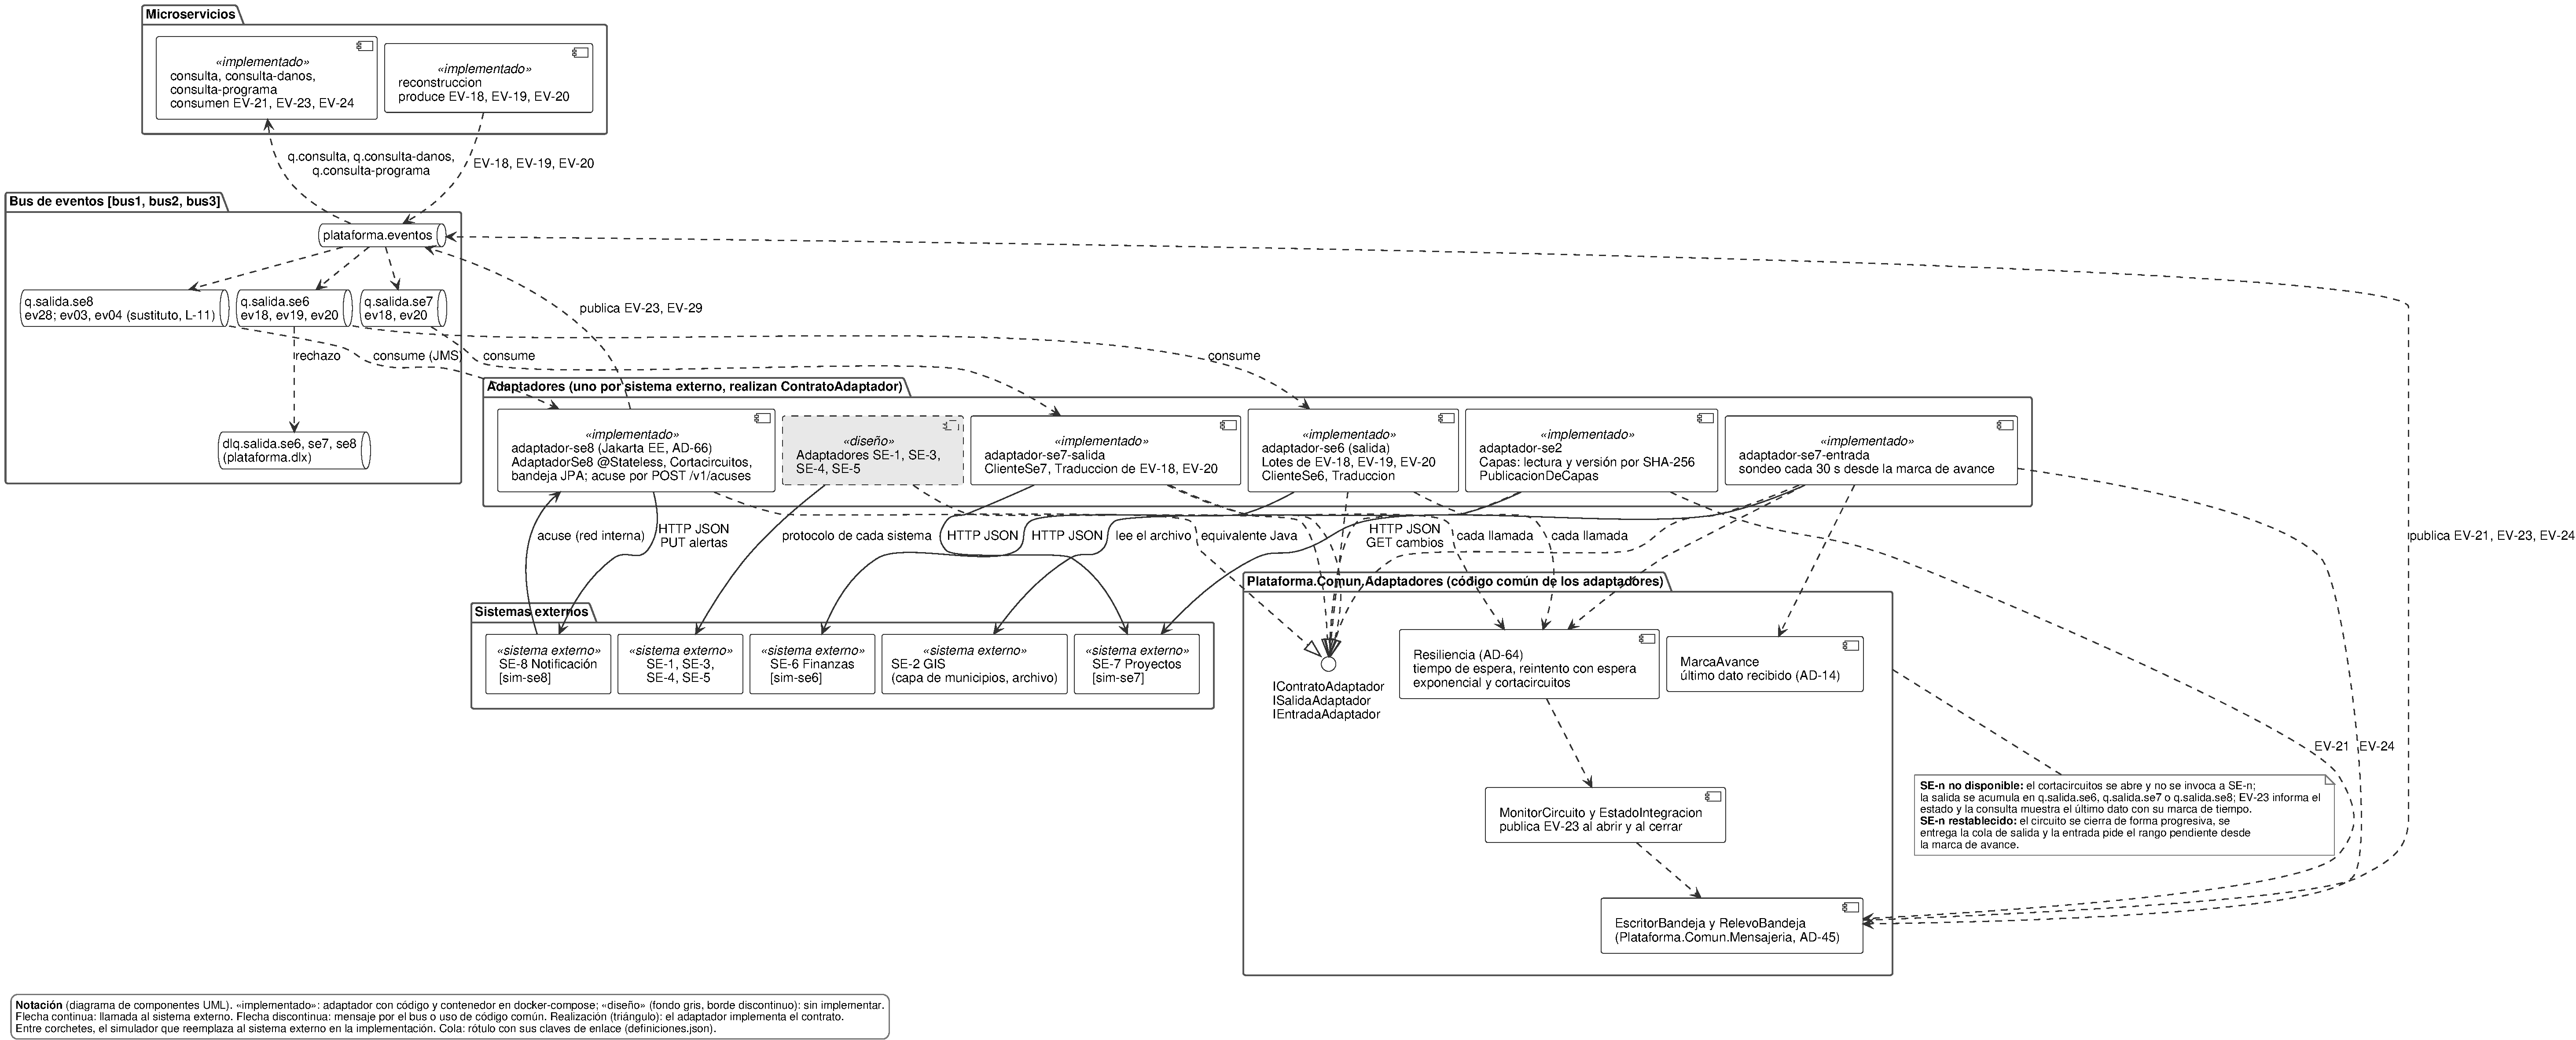
\includegraphics[width=\linewidth]{figuras/integracion}
\caption{Estructura común de una integración: adaptador, cortacircuitos, cola de salida y marca de
avance.}
\label{fig:integracion}
\end{figure}

Tres mecanismos se repiten en las integraciones:

\begin{itemize}
  \item Cortacircuitos por adaptador (AD-05, AD-37). Cada adaptador protege sus llamadas. La
        indisponibilidad de un sistema externo no afecta a las demás integraciones.
  \item Cola de salida con reintento asíncrono (AD-36). Los mensajes dirigidos a un sistema no
        disponible se encolan y se reintentan con espera creciente. La operación que los originó no
        espera.
  \item Marca de avance de entrada (AD-14). Cada adaptador registra el último dato recibido con
        éxito. Cuando la conexión se restablece, pide el rango pendiente. El consumo es idempotente
        por clave de origen, de modo que un dato reenviado se contabiliza una sola vez.
\end{itemize}

El comportamiento de cada integración difiere en la dirección, la frecuencia y la respuesta ante la
indisponibilidad. El \cref{tab:integracion} registra esas diferencias. Los protocolos se describen
como patrones de comunicación, porque los sistemas externos reales no están disponibles. En la
implementación, los adaptadores de SE-6 y SE-7 se comunican por HTTP con JSON con los simuladores
\texttt{sim-se6} y \texttt{sim-se7}, y el de SE-2 carga las divisiones administrativas de un
archivo GeoJSON (L-06). El de SE-8, en Jakarta EE (AD-66), se comunica por HTTP con JSON con
\texttt{sim-se8}. \enquote{Recepción por notificación}
indica que el sistema externo envía cuando ocurre un hecho. \enquote{Consulta periódica} indica que
el adaptador pregunta a intervalos. \enquote{API síncrona} indica una petición con respuesta
inmediata.

\begin{longtable}{L{2.2cm} L{2.4cm} L{2.4cm} L{3.3cm} L{4.8cm}}
\cabecera{5}{tab:integracion}{Integración con los sistemas externos}{\textbf{Sistema} &
\textbf{Protocolo} & \textbf{Formato} & \textbf{Patrón de comunicación} & \textbf{Comportamiento
ante indisponibilidad}}
SE-1 Alertas & Recepción por notificación. Consulta periódica como respaldo & Aviso del proveedor,
traducido al evento canónico & Solo entrada, asíncrono. El adaptador publica EV-01. No expone nada
hacia SE-1 & Cortacircuitos y marca de avance. El registro manual de un desastre sigue disponible
(RF-GD-02). Cuando SE-1 vuelve, se recupera el rango pendiente, ordenado por el instante del
fenómeno \\
SE-2 GIS & Consulta bajo demanda. Sincronización periódica de capas & Geometrías y divisiones
administrativas, traducidas a la geometría canónica & Bidireccional. Entrada de capas y zonas.
Salida de las delimitaciones y de su evolución & La caché de geometrías responde con la última
geometría calculada y su marca de tiempo (AD-17). El mapa no depende de la disponibilidad de SE-2.
La publicación de delimitaciones se encola \\
SE-3 Hospitalarios & Consulta periódica. Recepción por notificación de los cambios de capacidad &
Capacidad y atenciones, traducidas al evento canónico & Bidireccional, asíncrono. Entrada de
capacidad y personas atendidas. Salida de desastres activos y derivaciones & Es el escenario de
QA-01. La vista de capacidad muestra el último dato con su marca de tiempo. La salida se encola.
Cuando SE-3 vuelve, se sincroniza en ambos sentidos (\cref{fig:seq-eo3}) \\
SE-4 Recursos & Consulta periódica y recepción por notificación, con un adaptador por organismo &
Inventario del organismo, traducido al catálogo canónico & Bidireccional, asíncrono, con dos vías
de escritura (AD-35) & Cortacircuitos por organismo. La asignación se confirma en la plataforma sin
esperar a SE-4. Si el plazo vence sin respuesta, la reserva se libera (AD-39). La marca de avance
recupera los cambios de inventario \\
SE-5 Personas afectadas & API síncrona para la consulta puntual. Consulta periódica para la
actualización masiva & Registros de persona, con los campos sensibles marcados & Bidireccional.
Entrada de identificación y atención recibida. Salida de personas afectadas, necesidades y refugio &
Cortacircuitos y cola de salida. El adaptador cifra los campos personales en tránsito y la
plataforma los cifra en reposo (AD-23). El control de acceso se aplica antes de exponer un dato de
SE-5 (AD-22). Ante la indisponibilidad se degrada la consulta y se mantiene el control de acceso \\
SE-6 Financieros & Consulta periódica. Envío por lote & Presupuestos y ejecución, en formato
canónico & Bidireccional, asíncrono y de baja frecuencia & Cola de salida con reintento. El
historial de solo inserción permite reenviar la secuencia de cambios pendientes (AD-41). La
idempotencia usa la clave del proyecto y el número de versión \\
SE-7 Proyectos & Consulta periódica. Recepción por notificación de los avances & Estado, avance y
contratistas, en formato canónico & Bidireccional, asíncrono. Salida de proyectos creados. Entrada
de avance y contratista & Cortacircuitos, cola de salida y marca de avance. Un proyecto creado en
la plataforma queda registrado aunque SE-7 no esté disponible \\
SE-8 Notificación «implementado» & Envío por API: \texttt{PUT /v1/alertas/\{referencia\}}, idempotente
por referencia. Recepción por notificación de los acuses: \texttt{POST /v1/acuses}, una ruta solo de la
red interna que el gateway no enruta. Conciliación periódica con \texttt{GET /v1/acuses?desde=} desde
la marca de avance & Alerta de SE-8 (referencia, medio, destinatario, prioridad). Se traduce desde
EV-28 y, como sustituto temporal de Notificación, desde EV-03 y EV-04 (L-11) & Bidireccional,
asíncrono. Salida desde \texttt{q.salida.se8}. Entrada de acuses, que producen EV-29 solo para EV-28 &
Resiliencia del \cref{tab:tacticas-procesos}. Con SE-8 caído se abre el circuito, se publica EV-23 y
los mensajes esperan en la cola, sin ir a la DLQ. Cada alerta conserva su estado de entrega:
pendiente, enviada, entregada (solo con acuse, QA-08) o fallida. Sin acuse en \qty{5}{\second} se
reenvía con la misma referencia \\
\end{longtable}

En seis de las ocho integraciones la plataforma no es la fuente de los datos y replica información
que otro sistema administra (CON-1). Esto se refleja en dos elementos del diseño. El microservicio
de Consolidación conserva la procedencia de cada dato (AD-11) y la incluye en EV-02. El
microservicio de Gestión de Recursos registra el origen de cada recurso, externo o propio (AD-35),
y lo incluye en EV-12. Ambos microservicios aparecen en la vista lógica
(\cref{fig:vista-logica}). Los datos que se originan en la plataforma son la caracterización del
desastre, los proyectos de reconstrucción y los recursos que registran los organismos sin sistema
propio.

%==============================================================================
\section{Diseño de las principales APIs y eventos}
\label{sec:apis-eventos}

La plataforma tiene dos formas de interacción, como exige CON-5. Las APIs son síncronas: peticiones
con respuesta inmediata, que entran por el API Gateway y atienden los objetivos de latencia de QA-06
y QA-07. Los eventos son asíncronos: circulan por el bus, no bloquean al productor y toleran que un
consumidor no esté disponible, lo que atiende QA-01, QA-04 y QA-08. Ninguna función crítica invoca
de forma síncrona a un sistema externo (CON-3).

\subsection{Catálogo de APIs}
\label{sec:apis}

Todas las rutas se publican en el API Gateway (AD-04), que autentica, valida el rol, limita la tasa
por clase de tráfico y prioriza la consola de coordinación sobre el portal público (AD-19). El
microservicio de destino valida el token de nuevo y aplica sus reglas de autorización (AD-22,
AD-49). Los microservicios de consulta atienden las rutas de consulta (AD-15).

El \cref{tab:apis} lista las 56 rutas del catálogo \texttt{gateway/\br{}src/\br{}Plataforma.\br{}Gateway/\br{}rutas.\br{}json},
agrupadas por microservicio. Todas están implementadas. La columna Roles reproduce la metadata
\texttt{roles} del catálogo: \texttt{*} indica cualquier usuario autenticado y \texttt{publico}
indica una ruta sin token. Cuando la ruta tiene una regla de dominio de nivel 2
(\texttt{reglaDominio}), la descripción la nombra. El catálogo no admite rutas públicas de
modificación (R-07). El \cref{tab:apis-diseno} lista las rutas de los microservicios que quedan
como diseño (L-06).

Respecto de la versión 1.1 cambian cuatro puntos. El avance del proyecto se registra con
\texttt{POST /v1/proyectos/\{id\}/avance}, porque cada avance es un registro nuevo y no una
modificación (E-09). El mapa de daños es \texttt{GET /\br{}v1/\br{}consulta-\br{}danos/\br{}mapa} del microservicio de
consulta, y desaparece la ruta \texttt{/\br{}v1/\br{}mapa-\br{}calor} del primer prototipo (E-09). Las
candidatas de reconstrucción se leen de la copia local (AD-46, E-01). \texttt{POST /\br{}v1/\br{}desastres}
acepta un \texttt{id} generado por el cliente y es idempotente por ese identificador (AD-48, E-42).

\begingroup\small
\begin{longtable}{L{1.45cm} L{4.85cm} L{3.2cm} L{6.0cm}}
\cabecera{4}{tab:apis}{Catálogo de APIs implementadas (56 rutas del gateway)}{\textbf{Método} &
\textbf{Ruta} & \textbf{Roles} & \textbf{Descripción}}
\multicolumn{4}{@{}l}{\textbf{Gestión de Desastres} (\texttt{gestion-\br{}desastres}). Estado: «implementado»} \\
POST & \texttt{\br{}/v1\br{}/desastres} & \texttt{autoridad}, \texttt{organismo} & Registro de un
desastre desde la consola o desde el cliente móvil. Acepta un \texttt{id} del cliente: el reenvío
del mismo autor devuelve el desastre registrado y otro autor recibe 409 \texttt{ID\_EXISTE}
(AD-48). Publica EV-03 \\
GET & \texttt{\br{}/v1\br{}/desastres\br{}/\{id\}} & \texttt{*} & Estado vigente del desastre \\
PATCH & \texttt{\br{}/v1\br{}/desastres\br{}/\{id\}\br{}/severidad} & \texttt{autoridad},
\texttt{organismo} & Reclasificación de severidad con fila versionada. Publica EV-04. Regla
\texttt{organismo-\br{}responsable} (FP-03) \\
PUT & \texttt{\br{}/v1\br{}/desastres\br{}/\{id\}\br{}/zona} & \texttt{autoridad},
\texttt{organismo} & Delimitación geográfica. Publica EV-05. Regla
\texttt{organismo-\br{}responsable} \\
POST & \texttt{\br{}/v1\br{}/desastres\br{}/\{id\}\br{}/transiciones} & \texttt{autoridad},
\texttt{organismo} & Cambio de estado validado contra el perfil de ciclo de vida (RN-2). El cierre
exige 0 proyectos no finales (AD-47). Publica EV-06. Regla \texttt{organismo-\br{}responsable} \\
GET & \texttt{\br{}/v1\br{}/desastres\br{}/\{id\}\br{}/historial} & \texttt{*} & Evolución de
severidad, zona y estado, con autor e instante (AD-20) \\
GET & \texttt{\br{}/v1\br{}/desastres\br{}/\{id\}\br{}/organismos} & \texttt{*} & Organismo
responsable y participantes (RF-GD-12) \\
PUT & \texttt{\br{}/v1\br{}/desastres\br{}/\{id\}\br{}/organismos} & \texttt{autoridad},
\texttt{organismo} & Asigna el responsable y los participantes. Publica EV-27. Regla
\texttt{organismo-\br{}responsable} (E-35) \\
GET & \texttt{\br{}/v1\br{}/catalogos\br{}/tipos-desastre} & \texttt{*} & Catálogo de tipos y
niveles (AD-07) \\
POST & \texttt{\br{}/v1\br{}/catalogos\br{}/tipos-desastre} & \texttt{administrador} & Agrega un
tipo en ejecución (QA-10) \\
PATCH & \texttt{\br{}/v1\br{}/catalogos\br{}/tipos-desastre\br{}/\{codigo\}} &
\texttt{administrador} & Modifica un tipo \\
GET & \texttt{\br{}/v1\br{}/catalogos\br{}/tipos-desastre\br{}/\{codigo\}\br{}/ciclo-vida} &
\texttt{*} & Perfil de ciclo de vida del tipo con sus transiciones \\
GET & \texttt{\br{}/v1\br{}/catalogos\br{}/perfiles-ciclo-vida} & \texttt{*} & Perfiles de ciclo
de vida (E-35) \\
POST & \texttt{\br{}/v1\br{}/catalogos\br{}/perfiles-ciclo-vida} & \texttt{administrador} & Crea
un perfil en ejecución (RN-2, QA-10) \\
PUT & \texttt{\br{}/v1\br{}/catalogos\br{}/perfiles-ciclo-vida\br{}/\{codigo\}} &
\texttt{administrador} & Modifica un perfil. Un perfil en uso solo gana estados \\
GET & \texttt{\br{}/v1\br{}/catalogos\br{}/perfil-por-nivel} & \texttt{*} & Perfil mínimo de cada
nivel de severidad (RN-3) \\
PUT & \texttt{\br{}/v1\br{}/catalogos\br{}/perfil-por-nivel} & \texttt{administrador} & Modifica
el perfil mínimo por nivel \\
\multicolumn{4}{@{}l}{\textbf{Evaluación de Daños} (\texttt{evaluacion-\br{}danos}). Estado: «implementado»} \\
GET & \texttt{\br{}/v1\br{}/descarga} & \texttt{evaluador} & Descarga previa: catálogo, desastres no
cerrados y activos de la zona con su versión. Acepta \texttt{desastreId}, \texttt{zona} y
\texttt{desde} para la descarga incremental (RF-ED-12, AD-31, E-26, E-38) \\
POST & \texttt{\br{}/v1\br{}/sincronizacion\br{}/evaluaciones} & \texttt{evaluador} & Sincronización
por lote. Cada operación lleva su identificador y la versión base del activo. Detecta conflictos y
duplicados sin resolverlos y responde el resultado de cada operación (AD-32, AD-43, AD-44) \\
PUT & \texttt{\br{}/v1\br{}/evidencias\br{}/\{id\}} & \texttt{evaluador} & Carga una evidencia
declarada en el lote. Verifica el hash declarado (RF-ED-03) \\
GET & \texttt{\br{}/v1\br{}/evaluaciones} & \texttt{evaluador}, \texttt{operador},
\texttt{autoridad}, \texttt{organismo} & Evaluaciones, con filtro por dispositivo y por desastre
(E-09) \\
POST & \texttt{\br{}/v1\br{}/evaluaciones} & \texttt{evaluador} & Registro con conexión, con
desastre asociado o preliminar (AD-29) \\
PATCH & \texttt{\br{}/v1\br{}/evaluaciones\br{}/\{id\}} & \texttt{evaluador}, \texttt{operador} &
Actualización que conserva la versión anterior. Publica EV-26. Regla \texttt{dispositivo-\br{}autor} \\
POST & \texttt{\br{}/v1\br{}/evaluaciones\br{}/\{id\}\br{}/validacion} & \texttt{autoridad},
\texttt{organismo} & Valida o rechaza la evaluación. Publica EV-08. Regla
\texttt{organizacion-\br{}participante} (RF-ED-08) \\
POST & \texttt{\br{}/v1\br{}/evaluaciones\br{}/\{id\}\br{}/asociacion} & \texttt{operador},
\texttt{evaluador} & Vincula una evaluación preliminar a un desastre \\
GET & \texttt{\br{}/v1\br{}/conflictos} & \texttt{operador} & Bandeja de conflictos y de posibles
duplicados (E-13) \\
POST & \texttt{\br{}/v1\br{}/conflictos\br{}/\{id\}\br{}/resolucion} & \texttt{operador} & Elige la
versión que prevalece o fusiona un duplicado. Ninguna versión se elimina. Publica EV-22 (AD-32,
E-14) \\
GET & \texttt{\br{}/v1\br{}/catalogos\br{}/tipos-activo} & \texttt{*} & Tipos de activo y criterios
de daño (AD-28) \\
POST & \texttt{\br{}/v1\br{}/catalogos\br{}/tipos-activo} & \texttt{administrador} & Agrega un tipo
de activo en ejecución. Publica EV-25 (QA-10) \\
PATCH & \texttt{\br{}/v1\br{}/catalogos\br{}/tipos-activo\br{}/\{codigo\}} &
\texttt{administrador} & Modifica un tipo de activo. Publica EV-25 \\
\multicolumn{4}{@{}l}{\textbf{Consulta} (\texttt{consulta}). Estado: «implementado»} \\
GET & \texttt{\br{}/v1\br{}/consulta\br{}/desastres} & \texttt{*} & Tablero consolidado desde
proyecciones, con \texttt{datoAl} (FP-02, AD-16) \\
GET & \texttt{\br{}/v1\br{}/consulta\br{}/desastres\br{}/\{id\}} & \texttt{*} & Vista consolidada de
un desastre \\
GET & \texttt{\br{}/v1\br{}/consulta\br{}/desastres\br{}/\{id\}\br{}/evolucion} & \texttt{*} &
Evolución espacial y de severidad en el tiempo \\
GET & \texttt{\br{}/v1\br{}/consulta\br{}/mapa} & \texttt{*} & Mapa de desastres desde la caché de
geometrías (AD-17) \\
GET & \texttt{\br{}/v1\br{}/integraciones} & \texttt{*} & Estado de cada integración, alimentado por
EV-23 (R-10, E-15) \\
\multicolumn{4}{@{}l}{\textbf{Consulta de Daños} (\texttt{consulta-\br{}danos}). Estado: «implementado»} \\
GET & \texttt{\br{}/v1\br{}/consulta-danos\br{}/mapa} & \texttt{*} & Mapa de daños por zona (AD-34) \\
GET & \texttt{\br{}/v1\br{}/consulta-danos\br{}/consolidado} & \texttt{*} & Consolidado por zona y
por tipo de activo \\
GET & \texttt{\br{}/v1\br{}/consulta-danos\br{}/activos\br{}/\{id\}\br{}/evolucion} & \texttt{*} &
Evolución del daño de un activo \\
GET & \texttt{\br{}/v1\br{}/consulta-danos\br{}/zonas\br{}/\{codigo\}\br{}/evolucion} & \texttt{*} &
Evolución por municipio o departamento (RF-ED-15, E-40) \\
GET & \texttt{\br{}/v1\br{}/consulta-danos\br{}/indicadores-revision} & \texttt{*} & Indicadores de
la bandeja de revisión (R-08) \\
GET & \texttt{\br{}/tablero-danos\br{}/\{**resto\}} & \texttt{publico} & Tablero de daños en páginas
Razor con sesión OpenID Connect propia. La página autoriza (E-41) \\
\multicolumn{4}{@{}l}{\textbf{Reconstrucción} (\texttt{reconstruccion}). Estado: «implementado»} \\
GET & \texttt{\br{}/v1\br{}/reconstruccion\br{}/desastres} & \texttt{autoridad},
\texttt{responsable-\br{}proyecto}, \texttt{auditor} & Desastres de la copia local (AD-46) \\
GET & \texttt{\br{}/v1\br{}/reconstruccion\br{}/candidatas} & \texttt{autoridad} & Evaluaciones
validadas con daño grave o destrucción total, sin proyecto vigente, de la jurisdicción de la
autoridad. Se leen de la copia local alimentada por EV-03, EV-06, EV-08 y EV-21 (AD-46, E-01,
E-39) \\
POST & \texttt{\br{}/v1\br{}/proyectos:lote} & \texttt{autoridad} & Creación de proyectos por lote
(FP-08, AD-40). Publica EV-18. Regla \texttt{jurisdiccion-\br{}territorial} \\
GET & \texttt{\br{}/v1\br{}/proyectos} & \texttt{autoridad}, \texttt{responsable-\br{}proyecto},
\texttt{auditor} & Lista de proyectos, con filtro por desastre (E-09) \\
GET & \texttt{\br{}/v1\br{}/proyectos\br{}/\{id\}} & \texttt{autoridad},
\texttt{responsable-\br{}proyecto}, \texttt{auditor} & Detalle del proyecto \\
PATCH & \texttt{\br{}/v1\br{}/proyectos\br{}/\{id\}\br{}/presupuesto} & \texttt{autoridad} &
Presupuesto, fuente y cronograma. Inserta una fila en el historial y publica EV-19. Regla
\texttt{jurisdiccion-\br{}territorial} \\
PATCH & \texttt{\br{}/v1\br{}/proyectos\br{}/\{id\}\br{}/responsable} & \texttt{autoridad} & Asigna
el responsable del proyecto. Publica EV-20. Regla \texttt{jurisdiccion-\br{}territorial} (E-09) \\
POST & \texttt{\br{}/v1\br{}/proyectos\br{}/\{id\}\br{}/transiciones} & \texttt{autoridad},
\texttt{responsable-\br{}proyecto} & Cambio de estado del proyecto. Publica EV-20. Regla
\texttt{jurisdiccion-\br{}o-\br{}responsable-\br{}asignado} \\
POST & \texttt{\br{}/v1\br{}/proyectos\br{}/\{id\}\br{}/avance} & \texttt{responsable-\br{}proyecto} &
Registro de avance físico y costo ejecutado. Publica EV-20. Regla \texttt{responsable-\br{}asignado}
(E-09) \\
POST & \texttt{\br{}/v1\br{}/proyectos\br{}/\{id\}\br{}/documentos} & \texttt{responsable-\br{}proyecto}
& Documento de soporte en el almacén de objetos (RF-RC-06). Regla \texttt{responsable-\br{}asignado} \\
GET & \texttt{\br{}/v1\br{}/proyectos\br{}/\{id\}\br{}/historial} & \texttt{autoridad},
\texttt{auditor} & Historial de solo inserción (AD-41) \\
\multicolumn{4}{@{}l}{\textbf{Consulta del Programa} (\texttt{consulta-\br{}programa}). Estado: «implementado»} \\
GET & \texttt{\br{}/v1\br{}/programa\br{}/consolidado} & \texttt{autoridad}, \texttt{auditor} &
Consolidado por estado, presupuesto, costo ejecutado y avance (AD-42) \\
\multicolumn{4}{@{}l}{\textbf{Auditoría} (\texttt{auditoria}). Estado: «implementado»} \\
GET & \texttt{\br{}/v1\br{}/auditoria} & \texttt{auditor}, \texttt{autoridad} & Rastro por entidad,
actor o rango de fechas. No hay ruta de escritura (AD-21) \\
GET & \texttt{\br{}/v1\br{}/auditoria\br{}/huecos} & \texttt{auditor}, \texttt{autoridad} & Huecos
en la secuencia de cada productor (R-02, E-18) \\
\multicolumn{4}{@{}l}{\textbf{Consola de coordinación} (\texttt{web}). Estado: «implementado»} \\
GET, HEAD & \texttt{\br{}/\{**ruta\}} & \texttt{publico} & Archivos de la consola Angular. Es la
ruta de menor precedencia (AD-59) \\
\end{longtable}
\endgroup

\begingroup\small
\begin{longtable}{L{2.8cm} L{1.5cm} L{5.0cm} L{6.2cm}}
\cabecera{4}{tab:apis-diseno}{Catálogo de APIs de diseño, sin implementación (L-06)}{\textbf{Microservicio}
& \textbf{Método} & \textbf{Ruta} & \textbf{Descripción}}
Consolidación & GET & \texttt{\br{}/v1\br{}/reportes} & Reportes recibidos, con filtro por estado
de correlación y por confianza \\
Consolidación & POST & \texttt{\br{}/v1\br{}/correlaciones\br{}/\{id\}\br{}/decision} & El operador
confirma o rechaza una correlación de baja confianza (FP-04, AD-10) \\
Notificación & GET, POST, DELETE & \texttt{\br{}/v1\br{}/suscripciones} & Organismos que reciben
cada tipo de evento (AD-13) \\
Notificación & GET & \texttt{\br{}/v1\br{}/notificaciones\br{}/\{id\}} & Estado de entrega
(pendiente, entregada o fallida) y número de intentos \\
Gestión de Recursos & POST & \texttt{\br{}/v1\br{}/recursos} & Registro directo por un organismo
sin sistema propio. El recurso queda con origen interno \\
Gestión de Recursos & GET & \texttt{\br{}/v1\br{}/recursos} & Catálogo consolidado, con el origen y
la marca de tiempo de cada recurso \\
Gestión de Recursos & POST & \texttt{\br{}/v1\br{}/solicitudes-recurso} & Solicita una cantidad.
Responde con el estado reservado, sin esperar al sistema externo (FP-07) \\
Gestión de Recursos & GET & \texttt{\br{}/v1\br{}/solicitudes-recurso\br{}/\{id\}} & Estado de la
solicitud \\
Gestión de Recursos & POST & \texttt{\br{}/v1\br{}/donaciones} & Registro de una donación como
categoría del catálogo de recursos \\
Personas Afectadas & POST, GET, PATCH & \texttt{\br{}/v1\br{}/personas} & Registro y consulta de
personas y familias. Acceso por organización y campos cifrados (FP-10) \\
Personas Afectadas & POST & \texttt{\br{}/v1\br{}/personas\br{}/\{id\}\br{}/necesidades} &
Necesidades y solicitudes de ayuda \\
Personas Afectadas & POST, GET & \texttt{\br{}/v1\br{}/refugios\br{}/\{id\}\br{}/asignaciones} &
Ubicación de personas en refugios \\
Coordinación & POST, GET, PATCH & \texttt{\br{}/v1\br{}/tareas} & Tareas entre organismos, con
prioridad (FP-09) \\
Coordinación & GET & \texttt{\br{}/v1\br{}/desastres\br{}/\{id\}\br{}/actividades} & Historial de
actividades de los organismos \\
\end{longtable}
\endgroup
\subsection{Catálogo de eventos}
\label{sec:eventos}

Todos los eventos del bus usan el formato canónico (AD-09). El catálogo tiene 29 eventos, EV-01 a
EV-29, definidos en \texttt{comun/\br{}Plataforma.\br{}Comun.\br{}Eventos/\br{}CatalogoEventos.\br{}cs}, con un esquema JSON
por evento en \texttt{Esquemas/\br{}EV-\br{}nn.\br{}v1.\br{}json}. Todos comparten el sobre \texttt{sobre.v1.json}, con
los campos siguientes: \texttt{idEvento}, \texttt{tipo}, \texttt{nombre}, \texttt{version},
\texttt{instanteEmision}, \texttt{productor}, \texttt{secuenciaProductor}, \texttt{idCorrelacion},
\texttt{claveIdempotencia}, \texttt{procedencia} y \texttt{datos}.

Tres campos del sobre sustentan decisiones. El campo \texttt{claveIdempotencia} evita que un evento
entregado más de una vez se contabilice dos veces, lo que requieren las marcas de avance de AD-14 y
AD-37. El campo \texttt{procedencia} conserva la fuente del dato y su nivel de confianza (AD-11,
CON-1). El campo \texttt{secuenciaProductor} es un entero consecutivo por productor que asigna el
relevo de la bandeja solo a eventos confirmados. Con él Auditoría detecta huecos (R-02, E-18,
E-31).

El microservicio de Auditoría consume todos los eventos (AD-21), incluidos los tipos cuyo esquema
aún no conoce (E-34). Por brevedad, el \cref{tab:eventos} no lo repite en la columna de
consumidores. Todo evento se publica por medio de la bandeja de salida de su productor (AD-45).
La columna Productor marca con «diseño» los eventos cuyo productor no está implementado (L-06).
EV-07, EV-28 y EV-29 tienen esquema y colas declaradas para el diseño de Notificación, pero ningún
servicio implementado los produce ni los consume.

\begingroup\small
\begin{longtable}{L{1.1cm} L{2.7cm} L{2.4cm} L{2.9cm} L{6.2cm}}
\cabecera{5}{tab:eventos}{Catálogo de eventos}{\textbf{ID} & \textbf{Evento} & \textbf{Productor} &
\textbf{Consumidores} & \textbf{Campos principales}}
EV-01 & Reporte recibido & Adaptador de entrada (SE-1) «diseño» & Consolidación & \texttt{idReporte},
\texttt{sistemaOrigen}, \texttt{claveOrigen}, \texttt{tipoFenomeno}, \texttt{ubicacion},
\texttt{instanteFenomeno}, \texttt{severidadReportada}, \texttt{confianza} \\
EV-02 & Reporte consolidado & Consolidación «diseño» & Gestión de Desastres, Consulta &
\texttt{idCorrelacion}, \texttt{idsReportes}, \texttt{tipo}, \texttt{ubicacion},
\texttt{ventanaTemporal}, \texttt{procedencias}, \texttt{nivelConfianza},
\texttt{requiereConfirmacion} \\
EV-03 & Desastre creado & Gestión de Desastres & Notificación, Consulta, Evaluación de Daños,
Reconstrucción. Adaptador de SE-8 como sustituto (L-11) & \texttt{idDesastre}, \texttt{tipo}, \texttt{nombre}, \texttt{descripcion},
\texttt{severidad}, \texttt{zonaVersion}, \texttt{estado}, \texttt{instanteInicio},
\texttt{ubicacion}, \texttt{organismoRegistra}, \texttt{responsable}, \texttt{origen},
\texttt{versionDesastre} (E-30) \\
EV-04 & Severidad cambiada & Gestión de Desastres & Notificación, Consulta. Adaptador de SE-8 como
sustituto (L-11) & \texttt{idDesastre},
\texttt{severidadAnterior}, \texttt{severidadNueva}, \texttt{version}, \texttt{autor},
\texttt{motivo} \\
EV-05 & Zona actualizada & Gestión de Desastres & Consulta (invalida la caché de geometrías),
Evaluación de Daños & \texttt{idDesastre}, \texttt{zonaVersion}, \texttt{geometria},
\texttt{fuenteGeometria}, \texttt{autor} \\
EV-06 & Estado de desastre cambiado & Gestión de Desastres & Notificación, Consulta, Evaluación de
Daños, Reconstrucción & \texttt{idDesastre}, \texttt{estadoAnterior}, \texttt{estadoNuevo},
\texttt{autor}, \texttt{versionDesastre}. Dispara FP-08 cuando el estado nuevo es En
reconstrucción \\
EV-07 & Notificación despachada & Notificación «diseño» & Auditoría & \texttt{idNotificacion},
\texttt{idEventoOrigen}, \texttt{organismosDestino}, \texttt{canal}, \texttt{estadoEntrega},
\texttt{intentos}, \texttt{idDesastre}, \texttt{severidad}, \texttt{instanteAcuse} (E-37) \\
EV-08 & Evaluación validada & Evaluación de Daños & Consulta de Daños, Reconstrucción &
\texttt{idEvaluacion}, \texttt{idDesastre}, \texttt{tipoActivo}, \texttt{nivelDano},
\texttt{ubicacion}, \texttt{codigoMunicipio}, \texttt{estadoValidacion}, \texttt{evaluador},
\texttt{organizacion}, \texttt{version} (E-01, E-02) \\
EV-09 & Evaluación sincronizada & Evaluación de Daños & Consulta de Daños & \texttt{idEvaluacion},
\texttt{idDispositivo}, \texttt{instanteLocal}, \texttt{instanteServidor}, \texttt{enConflicto},
\texttt{versionesConservadas} \\
EV-10 & Conflicto o duplicado detectado & Evaluación de Daños & Consulta de Daños (marca en el mapa
e indicadores de revisión) & \texttt{idConflicto}, \texttt{idsEvaluaciones}, \texttt{idActivo},
\texttt{tipoConflicto}, \texttt{reglaDeteccion}, \texttt{versiones}, \texttt{estadoRevision}.
Ninguna versión se descarta (E-13) \\
EV-11 & Inventario actualizado & Adaptador de recursos (SE-4) «diseño» & Gestión de Recursos &
\texttt{idRecurso}, \texttt{organismo}, \texttt{categoria}, \texttt{cantidad}, \texttt{ubicacion},
\texttt{claveOrigen}, \texttt{marcaAvance} \\
EV-12 & Recurso registrado & Gestión de Recursos «diseño» & Consulta & \texttt{idRecurso},
\texttt{origen} (externo o propio), \texttt{organismo}, \texttt{categoria}, \texttt{cantidad} \\
EV-13 & Solicitud de confirmación de reserva & Gestión de Recursos «diseño» & Adaptador del
organismo dueño (SE-4) & \texttt{idSolicitud}, \texttt{idRecurso}, \texttt{cantidad},
\texttt{idDesastre}, \texttt{instanteExpiracion} \\
EV-14 & Reserva confirmada & Adaptador del organismo dueño «diseño» & Gestión de Recursos, Consulta
& \texttt{idSolicitud}, \texttt{cantidadConfirmada}, \texttt{instanteRespuesta} \\
EV-15 & Reserva rechazada & Adaptador del organismo dueño «diseño» & Gestión de Recursos, Consulta &
\texttt{idSolicitud}, \texttt{motivoRechazo}, \texttt{disponibilidadReal} \\
EV-16 & Reserva expirada & Gestión de Recursos «diseño» & Consulta & \texttt{idSolicitud},
\texttt{instanteExpiracion}, \texttt{cantidadLiberada}. Se emite cuando vence el plazo sin
respuesta (AD-39) \\
EV-17 & Recurso asignado & Gestión de Recursos «diseño» & Adaptador de salida (SE-4), Consulta &
\texttt{idSolicitud}, \texttt{idRecurso}, \texttt{cantidad}, \texttt{organismoDestino},
\texttt{idDesastre}, \texttt{autorizadoPor} \\
EV-18 & Proyecto creado & Reconstrucción & Consulta del Programa, Gestión de Desastres, adaptadores
de SE-6 y SE-7 & \texttt{idProyecto}, \texttt{idsEvaluacionesOrigen}, \texttt{idDesastre},
\texttt{presupuesto}, \texttt{fuenteFinanciacion}, \texttt{responsable}, \texttt{cronograma},
\texttt{codigosMunicipio}, \texttt{autor}, \texttt{proyecto} (E-30, E-33) \\
EV-19 & Presupuesto cambiado & Reconstrucción & Consulta del Programa, adaptador de SE-6 &
\texttt{idProyecto}, \texttt{tipoCambio}, \texttt{presupuestoAnterior}, \texttt{presupuestoNuevo},
\texttt{fuenteAnterior}, \texttt{fuenteNueva}, \texttt{versionHistorial}, \texttt{autor},
\texttt{justificacion}, \texttt{proyecto} \\
EV-20 & Estado o avance de proyecto cambiado & Reconstrucción & Consulta del Programa, Gestión de
Desastres, adaptadores de SE-6 y SE-7 & \texttt{idProyecto}, \texttt{estadoAnterior},
\texttt{estadoNuevo}, \texttt{avance}, \texttt{costoEjecutado}, \texttt{versionHistorial},
\texttt{autor}, \texttt{proyecto} (E-07, E-10) \\
EV-21 & Capa geográfica actualizada & Adaptador de SE-2 & Evaluación de Daños, Consulta, Consulta de
Daños, Gestión de Desastres, Reconstrucción & \texttt{capa}, \texttt{versionCapa},
\texttt{divisiones} (\texttt{codigo}, \texttt{nombre}, \texttt{codigoPadre}, \texttt{geometria}),
\texttt{fuente}, \texttt{parte}, \texttt{total} (E-11, E-36) \\
EV-22 & Conflicto o duplicado resuelto & Evaluación de Daños & Consulta de Daños &
\texttt{idConflicto}, \texttt{decision}, \texttt{idEvaluacionVigente}, \texttt{versionVigente},
\texttt{decididoPor}, \texttt{justificacion}, \texttt{evaluacion} (E-05) \\
EV-23 & Estado de integración cambiado & Adaptadores con cortacircuitos (implementados: SE-6, SE-7 y SE-8) & Consulta, Consulta
del Programa, Consulta de Daños & \texttt{sistemaExterno}, \texttt{estadoAnterior},
\texttt{estadoNuevo} (\texttt{CERRADO}, \texttt{ABIERTO}, \texttt{SEMIABIERTO}), \texttt{instante},
\texttt{mensajesEnCola} (E-15) \\
EV-24 & Avance o contratista reportado por SE-7 & Adaptador de SE-7 & Reconstrucción &
\texttt{idProyecto}, \texttt{tipo}, \texttt{avance}, \texttt{contratista},
\texttt{instanteExterno}, \texttt{claveOrigen}, \texttt{marcaAvance} (E-04) \\
EV-25 & Catálogo de tipos de activo actualizado & Evaluación de Daños & Consulta de Daños &
\texttt{codigo}, \texttt{nombre}, \texttt{criterios}, \texttt{version} (E-16) \\
EV-26 & Evaluación actualizada en el servidor & Evaluación de Daños & Consulta de Daños &
\texttt{idEvaluacion}, \texttt{motivo}, \texttt{autor}, \texttt{evaluacion} (E-06) \\
EV-27 & Organismos del desastre cambiados & Gestión de Desastres & Evaluación de Daños, Consulta &
\texttt{idDesastre}, \texttt{organismoResponsable}, \texttt{participantes}, \texttt{version},
\texttt{autor} (E-25) \\
EV-28 & Envío de notificación solicitado & Notificación «diseño» & Adaptador de SE-8 «implementado» &
\texttt{idNotificacion}, \texttt{intento}, \texttt{idEventoOrigen}, \texttt{idDesastre},
\texttt{organismo}, \texttt{canal}, \texttt{destino}, \texttt{asunto}, \texttt{mensaje},
\texttt{severidad} (E-37) \\
EV-29 & Acuse de notificación & Adaptador de SE-8 «implementado», solo para las alertas de EV-28 &
Notificación «diseño» &
\texttt{idNotificacion}, \texttt{intento}, \texttt{resultado} (\texttt{ENTREGADA} o
\texttt{FALLIDA}), \texttt{motivo}, \texttt{instante}, \texttt{claveOrigen} (E-37) \\
\end{longtable}
\endgroup

Los microservicios de Personas Afectadas y de Coordinación de Organismos publicarían sus eventos de
cambio con el mismo sobre, y el microservicio de Auditoría los consumiría (AD-21). El catálogo no
les asigna identificador porque ningún otro microservicio de dominio los consume.

\subsubsection{Topología del bus}
\label{sec:topologia-bus}

La topología se declara al desplegar, en \texttt{despliegue/\br{}bus/\br{}definiciones.\br{}json} (AD-02, AD-54).
Tiene tres intercambiadores:

\begin{itemize}
  \item \texttt{plataforma.\br{}eventos}, de tipo \emph{topic}. Cada evento se publica con la clave de
        ruteo \texttt{evNN.\br{}agregado.\br{}hecho}, por ejemplo \texttt{ev03.\br{}desastre.\br{}creado}. Cada cola se
        enlaza con el patrón \texttt{evNN.\#} de los eventos que consume.
  \item \texttt{plataforma.\br{}dlx}, que recibe los mensajes apartados de cada cola y los entrega a su
        cola \texttt{dlq.*} (E-23, E-32).
  \item \texttt{plataforma.\br{}sin-\br{}ruta}, que recibe los eventos sin cola de destino y los entrega a
        \texttt{q.sin-ruta} (E-23).
\end{itemize}

Todas las colas son de tipo quorum, replicadas en los tres nodos del bus. La política
\texttt{plataforma-\br{}colas} fija un límite de \num{100000} mensajes y \qty{256}{\mega\byte}, el
desborde \texttt{reject-\br{}publish} y un límite de cinco entregas (E-23). El \cref{tab:colas} lista las
colas.

\begingroup\small
\begin{longtable}{L{3.2cm} L{3.4cm} L{6.2cm} L{2.6cm}}
\cabecera{4}{tab:colas}{Colas del bus de eventos}{\textbf{Cola} & \textbf{Consumidor} &
\textbf{Eventos enlazados} & \textbf{Estado}}
\texttt{q.\br{}reconstruccion} & \texttt{reconstruccion} & EV-03, EV-06, EV-08, EV-21, EV-24 (AD-46) &
«implementado» \\
\texttt{q.\br{}consulta-\br{}programa} & \texttt{consulta-\br{}programa} & EV-18, EV-19, EV-20, EV-23 &
«implementado» \\
\texttt{q.\br{}consulta-\br{}danos} & \texttt{consulta-\br{}danos} & EV-08, EV-09, EV-10, EV-21, EV-22, EV-23,
EV-25, EV-26 & «implementado» \\
\texttt{q.consulta} & \texttt{consulta} & EV-03, EV-04, EV-05, EV-06, EV-21, EV-23, EV-27 &
«implementado» \\
\texttt{q.\br{}gestion-\br{}desastres} & \texttt{gestion-\br{}desastres} & EV-18, EV-20 (AD-47), EV-21 &
«implementado» \\
\texttt{q.\br{}evaluacion-\br{}danos} & \texttt{evaluacion-\br{}danos} & EV-03, EV-05, EV-06, EV-21, EV-27
(E-29) & «implementado» \\
\texttt{q.auditoria} & \texttt{auditoria} & Todos (\texttt{\#}) & «implementado» \\
\texttt{q.salida.se6} & \texttt{adaptador-se6} & EV-18, EV-19, EV-20 & «implementado» \\
\texttt{q.salida.se7} & \texttt{adaptador-\br{}se7-\br{}salida} & EV-18, EV-20 & «implementado» \\
\texttt{q.\br{}notificacion} & Notificación & EV-03, EV-04, EV-29 & Declarada para el diseño
(L-06) \\
\texttt{q.salida.se8} & \texttt{adaptador-se8} & EV-28. EV-03 y EV-04 como sustituto temporal de
Notificación (L-11) & «implementado» \\
\texttt{q.sin-ruta} & Operador (alarma) & Eventos sin cola de destino & «implementado» \\
\end{longtable}
\endgroup

Cada cola \texttt{q.*} tiene su cola de mensajes muertos con el mismo sufijo, por ejemplo
\texttt{dlq.\br{}reconstruccion}.

El \cref{tab:cobertura-fp} verifica que los diez casos de uso primarios y CU-4 se realizan con las
rutas del \cref{tab:apis,tab:apis-diseno} y los eventos del \cref{tab:eventos}.

\begin{longtable}{L{1.5cm} L{8.4cm} L{5.9cm}}
\cabecera{3}{tab:cobertura-fp}{Rutas y eventos que realizan cada caso de uso primario}{\textbf{ID} &
\textbf{Rutas} & \textbf{Eventos}}
FP-01 & Ninguna: la entrada es el adaptador de SE-1 «diseño». El registro manual usa
\texttt{POST /\br{}v1/\br{}desastres} & EV-01, EV-02, EV-03 \\
FP-02 & \texttt{/\br{}v1/\br{}consulta/\br{}*} & EV-03 a EV-06 alimentan las proyecciones \\
FP-03 & \texttt{/v1/desastres/\{id\}/severidad} y \texttt{/v1/desastres/\{id\}/zona} & EV-04,
EV-05 \\
FP-04 & \texttt{/v1/correlaciones/\{id\}/decision} & EV-01, EV-02 \\
FP-05 & \texttt{/\br{}v1/\br{}suscripciones} & EV-07 \\
FP-06 & \texttt{/v1/descarga}, \texttt{/\br{}v1/\br{}sincronizacion/\br{}evaluaciones},
\texttt{/v1/evidencias/\{id\}}, \texttt{/\br{}v1/\br{}conflictos} y
\texttt{/v1/evaluaciones/\{id\}/validacion} & EV-08, EV-09, EV-10, EV-22, EV-26 \\
FP-07 & \texttt{/\br{}v1/\br{}solicitudes-\br{}recurso} & EV-13 a EV-17 \\
FP-08 & \texttt{/\br{}v1/\br{}reconstruccion/\br{}candidatas}, \texttt{/\br{}v1/\br{}proyectos:\br{}lote} y
\texttt{/v1/proyectos/\{id\}/*} & EV-06 como disparador. EV-08 y EV-21 para la copia local. EV-18
a EV-20 y EV-24 \\
FP-09 & \texttt{/v1/desastres/\{id\}/organismos}, \texttt{/v1/tareas} y
\texttt{/v1/desastres/\{id\}/actividades} & Eventos de cambio hacia Auditoría \\
FP-10 & \texttt{/v1/personas}, \texttt{/v1/personas/\{id\}/necesidades} y
\texttt{/v1/refugios/\{id\}/asignaciones} & Eventos de cambio hacia Auditoría \\
CU-4 & \texttt{POST /\br{}v1/\br{}desastres} y \texttt{GET /\br{}v1/\br{}catalogos/\br{}tipos-\br{}desastre} & EV-03 \\
\end{longtable}

%==============================================================================
\section{Decisiones arquitectónicas documentadas}
\label{sec:decisiones}

Esta sección reúne las decisiones tomadas en las once iteraciones de ADD \cite{iteraciones}. Cada
fila consolida la decisión registrada en el paso 6 de su iteración con las alternativas evaluadas en
el paso 4.

El formato responde a CON-7. La columna de drivers cita el escenario \texttt{QA-nn}, el caso de uso
primario \texttt{FP-nn}, la regla \texttt{RN-n} o la restricción \texttt{CON-n} que respalda la
decisión. La última columna indica la justificación, la alternativa descartada y el costo aceptado.
Las decisiones estructurales se numeran de AD-01 a AD-49. Las decisiones de tecnología, AD-50 a
AD-66, están en la \cref{sec:tecnologia}.

Cuatro decisiones reutilizan un mecanismo ya decidido: AD-30, AD-34, AD-37 y AD-42. Se conservan
como decisiones porque la reutilización también se decidió frente a alternativas.

Las decisiones AD-43, AD-44 y AD-45 se agregan en la versión 1.1. Cierran el diseño de FP-06, que la
iteración 8 dejó abierto en tres puntos: la regla determinista de RF-ED-13 no estaba definida, la
cola del cliente no tenía reglas de retiro y de reenvío, y la publicación de los eventos de
sincronización no era atómica con la escritura. Estas decisiones no modifican ninguna decisión
anterior. El Anexo~\ref{sec:anexo-a} describe la implementación de FP-06.

La versión 1.2 agrega cuatro decisiones que surgieron al implementar. AD-46 corrige el origen de
las candidatas de reconstrucción: el SAD 1.1 decía que Reconstrucción las obtenía de Consulta de
Daños, lo que contradecía AD-01 (E-01, E-28). AD-47 da mecanismo a la regla de cierre del desastre
(E-07). AD-48 extiende el registro del desastre al cliente móvil en campo (E-42). AD-49 incorpora
el Proveedor de identidad a las vistas (E-43). La versión 1.2 también precisa dos decisiones. AD-42
se implementa como el mismo artefacto de Reconstrucción ejecutado como otro proceso. AD-45 se
extiende a todo productor de eventos (E-19). AD-46 a AD-49 no provienen de una iteración de ADD,
por lo que su columna It. no tiene número.

\begin{longtable}{L{1.15cm} L{3.5cm} L{0.7cm} L{1.9cm} L{8.0cm}}
\cabecera{5}{tab:decisiones}{Decisiones arquitectónicas consolidadas}{\textbf{ID} & \textbf{Decisión} &
\textbf{It.} & \textbf{Drivers} & \textbf{Justificación, alternativa descartada y costo aceptado}}
AD-01 & Dividir el sistema en microservicios, cada uno con su almacén & 1 & QA-02, QA-05, CON-4 &
Cada microservicio se escala, se despliega y falla por separado. Alternativa descartada: un
monolito en capas con base de datos compartida, en el que escalar la consulta obliga a replicar toda
la aplicación y un fallo puede detenerla completa. Costo aceptado: mayor complejidad de operación
y ausencia de consistencia inmediata entre microservicios \\
AD-02 & Comunicar los microservicios mediante un bus de eventos & 1 & QA-01, QA-04, QA-08, CON-5 &
El fallo de un consumidor no detiene al productor y el bus absorbe los picos de carga. Aplica las
tácticas de uso de un intermediario y de colas acotadas. Alternativa descartada: comunicación solo
síncrona entre microservicios. Costo aceptado: el flujo de control queda distribuido y es más
difícil de depurar \\
AD-03 & Un adaptador por cada sistema externo & 1 & QA-09, CON-2, CON-3 & Incorporar un sistema
externo consiste en agregar un adaptador, sin modificar los microservicios de dominio. Cada
adaptador aísla el fallo de su integración. AD-09 refina esta decisión con el contrato común \\
AD-04 & API Gateway como punto único de entrada & 1 & QA-11, QA-06 & Concentra la autenticación y
el control de tráfico en un solo lugar. Costo aceptado: todo el tráfico pasa por un componente, que
debe tener réplicas para no ser un punto único de fallo \\
AD-05 & Cortacircuitos con tiempo de espera, reintento y colas acotadas en las fronteras & 1 &
QA-01, QA-04, CON-3 & Limita la espera ante un componente que no responde y evita los fallos en
cascada. Los reintentos usan espera creciente. Costo aceptado: latencia adicional en el camino
degradado \\
AD-06 & Mantener el registro y la actualización del desastre en un solo microservicio & 2 & FP-01,
FP-03, QA-07 & Ambos casos de uso operan sobre la misma entidad y el mismo ciclo de vida.
Alternativa descartada: un microservicio por caso de uso, que obligaría a transferir la información
entre microservicios. Costo aceptado: el microservicio tiene dos responsabilidades \\
AD-07 & Catálogo de tipos de desastre y perfil de ciclo de vida como datos & 2 & QA-10, RN-1,
RN-2 & Incorporar un tipo de desastre no requiere modificar ni redesplegar componentes. Aplica la
táctica de enlace diferido por configuración. Alternativa descartada: una enumeración en el código,
que incumple QA-10. Costo aceptado: la validación se hace en ejecución y no en compilación \\
AD-08 & Organizar los elementos en cuatro capas: presentación, acceso, dominio e infraestructura &
2 & QA-10, CON-8 & Cada elemento nuevo tiene una ubicación definida. Una capa solo depende de las
inferiores, lo que limita el efecto de una modificación \\
AD-09 & Contrato común para todos los adaptadores, con evento canónico & 3 & QA-09, CON-1, CON-2 &
Cada adaptador resuelve su protocolo y todos entregan el mismo evento canónico. La plataforma
depende de una abstracción y no de ocho. Alternativas descartadas: una interfaz propia por
adaptador, que obligaría al dominio a conocer ocho formas de recibir información; y un adaptador
genérico configurable, que no cubre la heterogeneidad de los ocho sistemas. Costo aceptado: se
mantienen ocho adaptadores y un contrato cuyo cambio los afecta a todos \\
AD-10 & Correlación híbrida: clave de origen, ventana de espacio y tiempo, y confirmación del
operador & 3 & FP-04, RN-6 & La clave de origen descarta los reenvíos del mismo sistema. La ventana
correlaciona fuentes distintas. El operador confirma cuando la confianza es baja. Alternativas
descartadas: la clave de origen sola, que no correlaciona fuentes distintas; la ventana sola, que
puede unir dos eventos reales; y la confirmación manual en todos los casos, que no es viable con
cientos de reportes por minuto. Costo aceptado: parte de las correlaciones requiere una decisión
humana \\
AD-11 & Registrar la procedencia y el nivel de confianza de cada dato consolidado & 3 & QA-13,
CON-1, RN-6 & La procedencia es necesaria para consolidar, para resolver discrepancias y para
auditar. Es coherente con CON-1: la plataforma integra información de otros sistemas y no la
presenta como propia \\
AD-12 & Microservicio de Consolidación separado del de Gestión de Desastres & 3 & QA-05 & El
volumen de reportes es mucho mayor que el de desastres. La separación permite replicar la
consolidación sin replicar la gestión \\
AD-13 & Microservicio de Notificación con modelo de suscripciones & 3 & FP-05, QA-08, QA-10 & Los
demás microservicios no necesitan conocer los destinatarios. Incorporar un organismo consiste en
agregar una suscripción. Cada notificación conserva su estado de entrega \\
AD-14 & Marca de avance por adaptador para recuperar el flujo de entrada & 3 & QA-01, CON-3 &
Completa al cortacircuitos: cuando un sistema externo se restablece, el adaptador recupera el rango
pendiente. Costo aceptado: los datos recuperados se ordenan por el instante del hecho y no por el
orden de llegada \\
AD-15 & Separar el modelo de lectura del de escritura, con almacén propio alimentado por eventos &
4 & FP-02, QA-05, QA-07, CON-5 & Permite replicar la consulta sin replicar los microservicios de
escritura. Alternativas descartadas: leer los almacenes de otros microservicios, que rompe el
aislamiento de AD-01; y componer la respuesta con llamadas a cada microservicio de dominio, que
traslada la carga de consulta a la escritura. Costo aceptado: consistencia eventual, con un retraso
objetivo menor que \qty{2}{\second} \\
AD-16 & Mostrar la marca de tiempo del dato consultado & 4 & CON-6, QA-04 & Compensa el costo de
AD-15 y permite la degradación controlada: el usuario conoce la antigüedad del dato \\
AD-17 & Precalcular la geometría de las zonas y servirla desde una caché & 4 & QA-06 & La zona
cambia pocas veces y se consulta muchas. EV-05 sirve como señal de invalidación. Alternativas
descartadas: calcular la geometría en cada petición, que es la operación más costosa de la consulta;
y consultar a SE-2 en cada petición, que haría depender el mapa de un sistema externo. Costo
aceptado: espacio de almacenamiento y la invalidación de la caché \\
AD-18 & Más réplicas del microservicio de Consulta que de los de escritura & 4 & QA-05, CON-4 & La
carga es asimétrica: miles de usuarios consultan y decenas registran. Replicar todos los
microservicios por igual asignaría capacidad donde no se requiere \\
AD-19 & Priorización y degradación controlada en el API Gateway según el tipo de cliente & 4 &
QA-04, CON-6 & Ante un exceso de carga se degrada primero el portal público y se preserva la consola
de coordinación. Se devuelve una respuesta reducida en lugar de un error. Costo aceptado: menor
calidad de servicio para el ciudadano durante el pico \\
AD-20 & Historial versionado, con una fila nueva por cambio & 5 & FP-03, QA-13, QA-15, RN-4 &
Permite consultar la evolución del desastre sin reconstruir el estado vigente a partir de eventos.
Alternativas descartadas: sobrescribir el estado y llevar una tabla de auditoría aparte, que
mantiene dos representaciones del mismo hecho; y el almacenamiento por eventos (\emph{event
sourcing}), que excede la necesidad y obligaría a replantear AD-06. Costo aceptado: la consulta de
la evolución lee y ordena varias filas \\
AD-21 & Microservicio de Auditoría centralizado, alimentado por el bus, con registro inmutable e
idempotente & 5 & QA-13, QA-15, CON-7 & Una consulta reconstruye el rastro completo de una acción,
con independencia de los microservicios que intervinieron. Alternativa descartada: un registro por
microservicio, que obligaría a consultar varios almacenes. Costo aceptado: un componente adicional
que no debe perder eventos \\
AD-22 & Autorización en dos niveles: rol y organización en el API Gateway, y reglas específicas en
cada microservicio & 5 & QA-11, FP-09, FP-10 & Cualquier usuario con el rol adecuado puede consultar
un desastre, pero solo el organismo responsable puede modificar su severidad o su zona. Esa regla
depende de datos que solo tiene el microservicio de dominio. Alternativas descartadas: autorizar
solo en cada microservicio, que duplica la validación común; y autorizar solo en el API Gateway,
que no conoce los datos del dominio. Costo aceptado: el control de acceso se verifica en dos
lugares \\
AD-23 & Cifrado por columna de los datos de contacto y de los campos identificatorios & 5 & QA-12,
FP-10 & Se cifran los campos sensibles: los datos de contacto del responsable y de los organismos, y
los campos identificatorios de las personas afectadas. Alternativa descartada: cifrar los almacenes
completos, que aumenta el costo de cada consulta sin proteger más los campos no sensibles. Costo
aceptado: el tratamiento de los campos no es uniforme \\
AD-24 & Réplica activa local (\emph{hot spare}) con sondeo de salud & 6 & QA-02, QA-04 & Ante el
fallo de una instancia, las réplicas activas asumen la carga sin interrupción. Reutiliza las
réplicas creadas para la escalabilidad. Alternativas descartadas: el reinicio manual, que no es
viable durante una emergencia; y la reposición automática sin réplica activa, que deja un intervalo
sin servicio. Costo aceptado: recursos adicionales y coordinación entre réplicas \\
AD-25 & Modelo híbrido de ejecución: microservicios persistentes y adaptadores efímeros & 6 & QA-05,
QA-08, CON-4, CON-8 & Los microservicios de dominio deben responder de inmediato. Los adaptadores
traducen de forma puntual y están inactivos la mayor parte del tiempo. Alternativas descartadas:
capacidad fija administrada manualmente, que no absorbe el paso de \num{1000} a \num{10000}
usuarios; y unidades efímeras para todos los componentes, cuyo tiempo de arranque compromete QA-08.
Riesgo declarado: si el arranque de un adaptador compromete los \qty{5}{\second} de una alerta
crítica, se mantiene una instancia encendida \\
AD-26 & Dos regiones, con réplica en espera (\emph{warm spare}) y conmutación automática & 6 &
QA-03, QA-02 & Mantiene el servicio ante un siniestro regional que inutilice la sede principal.
Alternativas descartadas: un solo centro de cómputo; y varias sedes en la misma ciudad, que no
protegen ante un sismo regional. Costo aceptado: un RPO $\le$ \qty{60}{\second} por la replicación
asíncrona, que se elige para no aumentar la latencia de escritura \\
AD-27 & Resincronización de estado al reincorporar la sede primaria & 6 & QA-03 & Los datos de la
sede recuperada convergen con los de la sede activa antes de que reciba tráfico \\
AD-28 & Catálogo de tipos de activo y de criterios de daño en el microservicio de Evaluación de
Daños & 7 & QA-10, RN-5 & Las cinco categorías de daño son fijas y los criterios varían por tipo de
activo. Alternativas descartadas: una enumeración en el código; y un catálogo compartido en Gestión
de Desastres, que rompe el aislamiento de AD-01. Costo aceptado: el patrón de catálogo se repite en
dos microservicios \\
AD-29 & Registro preliminar de la evaluación, con asociación posterior al desastre & 7 & FP-06 &
Permite registrar en campo cuando aún no se identifica el evento. Un operador hace la asociación
después. Alternativas descartadas: exigir siempre un desastre asociado; y la asociación automática
por coincidencia geográfica y temporal, cuyo error tiene mayor costo que una evaluación pendiente.
Costo aceptado: la evaluación queda sin asociar hasta su revisión \\
AD-30 & Actualización de evaluaciones con el historial versionado de AD-20 & 7 & QA-13 & Reutiliza
el mecanismo de AD-20, porque el problema es el mismo: conservar la evolución de un dato \\
AD-31 & Réplica local completa en el cliente móvil, con sincronización diferida & 8 & FP-06, QA-14,
CON-6 & Permite al evaluador leer y escribir sin conexión. Alternativa descartada: una cola local
de solo escritura, que no permite consultar la información descargada. Costo aceptado: los
conflictos se tratan al sincronizar \\
AD-32 & La regla determinista solo detecta el conflicto. Se conservan ambas versiones y decide un
usuario autorizado & 8 & QA-14, CON-6 & La plataforma no decide qué versión de un dato prevalece.
Alternativas descartadas: la resolución automática, por ejemplo conservar el daño más alto; y la
regla de la última escritura, que no garantiza que prevalezca el valor correcto. Costo aceptado: la
evaluación queda pendiente de revisión \\
AD-33 & Detección de evaluaciones duplicadas por ventana de tiempo configurable, con fusión o
rechazo por un usuario & 8 & QA-14 & Aplica el principio de AD-32 a las evaluaciones independientes
sobre el mismo activo. Alternativa descartada: la fusión automática dentro de la ventana. Costo
aceptado: dos evaluaciones legítimas pueden marcarse como posible duplicado si la ventana es
amplia. Por eso la ventana es configurable \\
AD-34 & Microservicio de Consulta de Daños con modelo de lectura propio & 8 & QA-06, QA-05 &
Reutiliza AD-15: el consolidado por zona y por tipo de activo y el mapa se atienden con
proyecciones alimentadas por eventos \\
AD-35 & Catálogo de recursos con dos vías de escritura (adaptadores y registro directo), con el
origen de cada recurso & 9 & FP-07, CON-1 & Cubre a los organismos con sistema de inventario y a los
que no lo tienen. Para los recursos externos la plataforma es una réplica. Para los registrados
directamente es la fuente. Alternativas descartadas: solo adaptadores, que excluye a los organismos
sin sistema; y solo registro directo, que renuncia a la integración. Costo aceptado: hay dos caminos
de escritura \\
AD-36 & Publicación hacia los sistemas externos por cola, con reintento asíncrono y espera
creciente & 9 & QA-01, CON-3, CON-5 & La asignación se confirma en la plataforma sin esperar al
sistema externo. El mensaje pendiente se entrega cuando el sistema vuelve. Alternativas
descartadas: el reintento síncrono, que bloquea una operación crítica; y fallar con notificación al
organismo, que deja la asignación sin reintento. Costo aceptado: la confirmación visible para el
organismo dueño puede demorarse \\
AD-37 & Cortacircuitos por adaptador y marca de avance del inventario recibido & 9 & QA-01, CON-3 &
Reutiliza AD-05 y AD-14. La indisponibilidad de un organismo no afecta la integración con los
demás. La idempotencia usa la clave de origen de cada movimiento \\
AD-38 & Modelo de cantidad con reserva temporal & 10 & FP-07 & Los recursos se miden en cantidad.
La reserva evita la sobreasignación ante solicitudes concurrentes. Alternativas descartadas: la
unidad indivisible, que no sirve para recursos medidos en cantidad; y el descuento directo sin
reserva, en el que dos solicitudes pueden leer la misma disponibilidad. Costo aceptado: debe
definirse qué ocurre si la confirmación no llega \\
AD-39 & Confirmación asíncrona de la reserva con plazo de expiración & 10 & FP-07, QA-01, CON-5 &
La reserva y la confirmación son dos pasos. La operación no depende de la respuesta del sistema
externo. Si el plazo vence, la reserva se libera. Alternativa descartada: la confirmación síncrona
contra el adaptador al reservar. Costo aceptado: una solicitud puede tardar hasta el plazo en
conocerse como rechazada \\
AD-40 & Disparador por la transición del desastre a En reconstrucción, con creación de proyectos
por lote & 11 & FP-08, RN-2 & El disparador es el estado formal del desastre y la operación acepta
un conjunto de evaluaciones. Alternativa descartada: crear un proyecto por cada evaluación con daño
grave, que no admite lotes y crea proyectos antes de la fase de reconstrucción. Costo aceptado: no
hay proyectos antes de la transición \\
AD-41 & Historial de solo inserción para el presupuesto y el estado del proyecto & 11 & QA-15,
QA-13 & Reutiliza el historial de AD-20 y agrega la garantía de inmutabilidad: el almacén no admite
actualización ni borrado. Alternativa descartada: el historial versionado con actualización
habilitada. Costo aceptado: una corrección se registra como una entrada nueva \\
AD-42 & Microservicio de Consulta del Programa con modelo de lectura propio & 11 & QA-06, QA-05 &
Reutiliza AD-15 y AD-34: el consolidado del programa se atiende con proyecciones alimentadas por
eventos. Se implementa como el mismo artefacto, otro proceso: \texttt{consulta-\br{}programa} ejecuta la
imagen de Reconstrucción con \texttt{Reconstruccion\_\br{}\_\br{}Rol=consulta}, con su propia base
(\texttt{programa}), su cola \texttt{q.\br{}consulta-\br{}programa} y sus réplicas. Alternativa descartada: un
proyecto y una imagen aparte, que duplican el código de lectura del mismo agregado. Costo aceptado:
un cambio en la imagen redespliega los dos procesos \\
AD-43 & Regla determinista de conflicto: hay conflicto si el activo tiene una versión mayor que la
versión base de la operación, producida por otro dispositivo & 8 & QA-14, RF-ED-13 & Cada operación
del cliente declara la versión del activo que el dispositivo conocía. Todo cambio de otro
dispositivo aumenta la versión, de modo que se detecta siempre: 0 falsos negativos, como pide la respuesta de QA-14. Las
secuencias de crear y luego editar de un mismo dispositivo sin conexión no se marcan como conflicto.
Alternativas descartadas: comparar solo el número de versión, que produce falsos positivos en esas
secuencias; y comparar marcas de tiempo, que depende de los relojes de los dispositivos y no cumple
S-5. Costo aceptado: el microservicio conserva, por cada versión del activo, el dispositivo que la
produjo \\
AD-44 & Cola local de operaciones inmutables, con copia completa del contenido al encolar & 8 &
QA-14 & Una operación solo sale de la cola cuando el servidor responde por ella, lo que evita
pérdidas (medida de QA-14). El reenvío es idempotente por identificador de operación: el servidor guarda el
resultado de cada operación y lo devuelve ante un reenvío, sin crear registros, como pide la respuesta de QA-14.
Alternativa descartada: enviar el estado vigente de la réplica local al sincronizar, que pierde las
ediciones intermedias y no permite un reenvío idempotente. Costo aceptado: espacio en el
dispositivo y un registro de operaciones procesadas en el servidor \\
AD-45 & Bandeja de salida transaccional en todo microservicio productor & 8 & RF-ED-14, QA-04,
QA-15 & Todo microservicio que publica eventos de cambio los escribe en su bandeja de salida, en la
misma transacción que el cambio, y un relevo los envía al bus después (E-19). La versión 1.1 la
aplicaba solo a EV-09 y EV-10. Si el bus no está disponible, el evento permanece en la bandeja: 0
eventos perdidos y 0 cambios sin registro, como piden las respuestas de QA-04 y QA-15. El relevo asigna la secuencia del
productor (E-31). Alternativa descartada: publicar en el bus después de confirmar la transacción,
que pierde el evento si el proceso falla entre ambos pasos. Costo aceptado: la entrega es al menos
una vez, por lo que los consumidores deben ser idempotentes (AD-02) \\
AD-46 & Reconstrucción mantiene copias locales de desastres, evaluaciones validadas y municipios,
alimentadas por eventos & -- & QA-04, QA-06, RF-RC-01, FP-08 & Las candidatas y los proyectos se
calculan con las copias locales de EV-03 y EV-06 (desastres), EV-08 (evaluaciones validadas) y
EV-21 (municipios), que llegan por \texttt{q.\br{}reconstruccion} (E-01, E-28, E-36). Reconstrucción
responde aunque Evaluación de Daños o Consulta de Daños no estén disponibles. Alternativa
descartada: la llamada síncrona a Consulta de Daños que describía el SAD 1.1, que crea una
dependencia en ejecución entre microservicios y contradice AD-01. Costo aceptado: consistencia
eventual, con un retraso objetivo menor que \qty{2}{\second}, y la copia de datos de otro módulo
(CON-1) \\
AD-47 & Gestión de Desastres consume EV-18 y EV-20 para impedir el cierre de un desastre con
proyectos abiertos & -- & RN-2, RF-GD-07 & Gestión de Desastres cuenta los proyectos no finales de
cada desastre con los eventos de \texttt{q.\br{}gestion-\br{}desastres}. La transición a Cerrado exige que
el contador sea 0 (E-07). Alternativa descartada: consultar a Reconstrucción de forma síncrona al
cerrar, que es una dependencia síncrona entre microservicios (AD-01). Costo aceptado: un proyecto
recién finalizado tarda menos de \qty{2}{\second} en permitir el cierre \\
AD-48 & Registro del desastre en campo desde el cliente móvil, con cola local e identificador
generado en el cliente & -- & RF-GD-02, RF-GD-03, RF-GD-05, RF-GD-08, QA-07, AD-44 & El cliente
guarda el registro en su base local y lo envía cuando hay conexión. \texttt{POST /\br{}v1/\br{}desastres} es
idempotente por el \texttt{id} del cliente: el reenvío del mismo autor devuelve el desastre ya
registrado y otro autor recibe 409 (E-42). Aplica a los desastres las reglas de retiro y de reenvío
de AD-44. Alternativas descartadas: registrar solo con conexión, que impide caracterizar un
desastre en una zona sin red; y asignar el identificador en el servidor, que duplica el desastre
si la respuesta se pierde y el cliente reenvía. Costo aceptado: el servidor debe rechazar un
\texttt{id} que ya pertenece a otro autor \\
AD-49 & Proveedor de identidad federado externo, con OpenID Connect y PKCE, y validación del token
en el API Gateway y en cada microservicio & -- & QA-11, AD-04, AD-22 & Los usuarios se autentican
en un proveedor externo. El API Gateway valida la firma, el emisor, la audiencia y el rol del token
(nivel 1). Cada microservicio valida el mismo token y aplica la regla de dominio (nivel 2), de modo
que una petición que evita el gateway también se rechaza (E-43). Alternativas descartadas: una
identidad propia en cada microservicio, que duplica credenciales; y validar solo en el gateway, que
deja sin protección la red interna. Costo aceptado: un componente externo más y la validación del
token en dos lugares \\
\end{longtable}

\subsection{Cobertura de los drivers}
\label{sec:cobertura}

El \cref{tab:cobertura-decisiones} relaciona cada driver con las decisiones que lo atienden. Cubre
los quince escenarios de atributo de calidad, los diez casos de uso primarios y las ocho
restricciones del SRS. CON-7 no se asocia a una decisión, porque es la restricción que define el
formato del \cref{tab:decisiones}.

La versión 1.1 actualiza cuatro filas. QA-14 y FP-06 incorporan AD-43, AD-44 y AD-45. QA-04
incorpora AD-45. Se agregan las filas de FP-09 y FP-10. La versión 1.2 incorpora AD-46 a AD-49 y
la fila de CON-8 remite a la \cref{sec:tecnologia}. Los atributos que favorece cada decisión de
tecnología están en el \cref{tab:tecnologia-resumen}.

\begin{longtable}{L{2.0cm} L{13.8cm}}
\cabecera{2}{tab:cobertura-decisiones}{Trazabilidad inversa: de cada driver a las decisiones que lo
atienden}{\textbf{Driver} & \textbf{Decisiones}}
QA-01 & AD-02, AD-05, AD-14, AD-36, AD-37, AD-39 \\
QA-02 & AD-01, AD-24, AD-26 \\
QA-03 & AD-26, AD-27 \\
QA-04 & AD-02, AD-05, AD-16, AD-19, AD-24, AD-45, AD-46 \\
QA-05 & AD-01, AD-12, AD-15, AD-18, AD-25, AD-34, AD-42 \\
QA-06 & AD-04, AD-17, AD-23, AD-34, AD-42, AD-46 \\
QA-07 & AD-06, AD-15, AD-48 \\
QA-08 & AD-02, AD-13, AD-25 \\
QA-09 & AD-03, AD-09 \\
QA-10 & AD-07, AD-08, AD-13, AD-28 \\
QA-11 & AD-04, AD-22, AD-49 \\
QA-12 & AD-23 \\
QA-13 & AD-11, AD-20, AD-21, AD-30, AD-41 \\
QA-14 & AD-31, AD-32, AD-33, AD-43, AD-44 \\
QA-15 & AD-20, AD-21, AD-41, AD-45 \\
\midrule
FP-01 & AD-06, AD-48 \\
FP-02 & AD-15 \\
FP-03 & AD-06, AD-20 \\
FP-04 & AD-10 \\
FP-05 & AD-13 \\
FP-06 & AD-29, AD-31, AD-43, AD-44, AD-45 \\
FP-07 & AD-35, AD-38, AD-39 \\
FP-08 & AD-40, AD-41, AD-46, AD-47 \\
FP-09 & AD-22 \\
FP-10 & AD-22, AD-23 \\
\midrule
CON-1 & AD-09, AD-11, AD-35, AD-46 \\
CON-2 & AD-03, AD-09 \\
CON-3 & AD-03, AD-05, AD-14, AD-36, AD-37 \\
CON-4 & AD-01, AD-18, AD-25 \\
CON-5 & AD-02, AD-15, AD-36, AD-39 \\
CON-6 & AD-16, AD-19, AD-31, AD-32, AD-46, AD-48 \\
CON-7 & Define el formato del \cref{tab:decisiones} \\
CON-8 & Entrega 1: AD-08, AD-25, AD-26. Entrega 2: sustituida por AD-50 a AD-65
(\cref{sec:tecnologia}) \\
CON-9 & AD-03, AD-50, AD-66 \\
\end{longtable}

%==============================================================================
%==============================================================================
%  Decisiones de tecnología (SAD v1.2). Archivo incluido desde main.tex con %==============================================================================
%  Decisiones de tecnología (SAD v1.2). Archivo incluido desde main.tex con %==============================================================================
%  Decisiones de tecnología (SAD v1.2). Archivo incluido desde main.tex con \input{tecnologia}.
%  Generado a partir de la especificación de la versión 1.2. No carga paquetes.
%==============================================================================
\section{Decisiones de tecnología}
\label{sec:tecnologia}

El enunciado del proyecto (§8) pide seleccionar las tecnologías en la segunda entrega.
CON-8 exigía independencia tecnológica en la primera entrega.
Esta sección sustituye esa condición para la segunda entrega.
El Anexo~\ref{sec:anexo-a} deja de ser una excepción a CON-8 y describe la implementación de FP-06 con las tecnologías elegidas aquí.

Las decisiones se numeran de AD-50 a AD-66.
AD-66 responde a CON-9, que se agregó después de AD-50 a AD-65.
Ninguna modifica una decisión estructural.
Cada una materializa uno o varios mecanismos de AD-01 a AD-49, y su justificación parte de los escenarios QA-nn que ese mecanismo debe cumplir (CON-7).

\subsection{Método de decisión}
\label{sec:tec-metodo}

Cada decisión sigue cinco pasos:
\begin{enumerate}
  \item Se identifica el mecanismo del SAD que la tecnología materializa y los escenarios QA-nn que ese mecanismo atiende.
  \item Se eligen entre tres y cinco alternativas con uso real para ese mecanismo.
  \item Se definen los criterios. Cada criterio cita el QA-nn, AD-nn o CON-n del que proviene. La experiencia del equipo y la licencia o el costo se incluyen con un peso menor que los criterios de calidad.
  \item Se asigna un peso a cada criterio. Los pesos de una decisión suman 100\,\%.
  \item Se califica cada alternativa en cada criterio y se calcula el total ponderado.
\end{enumerate}

La escala de calificación tiene cinco niveles:
\begin{itemize}
  \item 1: la alternativa no satisface el criterio o lo impide.
  \item 2: lo satisface con desarrollo propio considerable.
  \item 3: lo satisface con configuración adicional o con complementos de terceros.
  \item 4: lo satisface de forma nativa con limitaciones menores.
  \item 5: lo satisface de forma nativa y la implementación lo verifica.
\end{itemize}

El total ponderado de una alternativa es $\sum_i p_i \, c_i / 100$, donde $p_i$ es el peso en porcentaje y $c_i$ la calificación del criterio $i$.
El máximo es 5.
Las cifras de verificación citadas provienen del perfil local de un computador, con 20 clientes, y no reemplazan la prueba con 10\,000 usuarios (L-04).

\subsection{Resumen de las decisiones}
\label{sec:tec-resumen}

El \cref{tab:tecnologia-resumen} relaciona cada decisión con su tecnología, el mecanismo que materializa y los escenarios que favorece.
Las versiones son las de los archivos de proyecto.

\begingroup\small
\begin{longtable}{L{1.15cm} L{2.2cm} L{6.0cm} L{2.6cm} L{2.6cm}}
\cabecera{5}{tab:tecnologia-resumen}{Resumen de las decisiones de tecnología}{\textbf{ID} & \textbf{Categoría} &
\textbf{Tecnología y versión} & \textbf{Mecanismo} & \textbf{QA que favorece}}
AD-50 & Lenguaje y plataforma & C\# sobre .NET 10 (SDK 10.0.100, \texttt{net10.0}) & AD-01, AD-08, AD-09, AD-45 & QA-06, QA-07, QA-14 \\
AD-51 & Marco web & ASP.NET Core 10 (controladores y \emph{minimal APIs}) & AD-08, AD-22, AD-24 & QA-06, QA-07, QA-11 \\
AD-52 & Persistencia & PostgreSQL 18 con PostGIS 3.6 (\texttt{postgis/postgis:18-3.6}), una base por microservicio y réplica \texttt{db-replica} & AD-01, AD-17, AD-20, AD-24, AD-41, AD-45 & QA-03, QA-04, QA-06, QA-13, QA-15 \\
AD-53 & Acceso a datos & Entity Framework Core 10.0.14, Npgsql 10.0.3 y NetTopologySuite 10.0.3, con contenedor migrador & AD-08, AD-17, AD-41, AD-45 & QA-06, QA-10, QA-13 \\
AD-54 & Mensajería & RabbitMQ 4.4 (3 nodos, colas quorum acotadas, DLQ) con RabbitMQ.Client 7.2.2 & AD-02, AD-05, AD-36, AD-45 & QA-01, QA-04, QA-08 \\
AD-55 & Caché & Redis 8.8 (\texttt{redis:8.8.4-alpine}) con StackExchange.Redis 3.4.29 & AD-16, AD-17 & QA-05, QA-06 \\
AD-56 & Almacén de objetos & MinIO con API S3 (paquete Minio 7.0.0) & AD-24, AD-31 & QA-02, QA-03, QA-14 \\
AD-57 & Puerta de entrada & YARP 2.3.0 con catálogo \texttt{rutas.json} (56 rutas) & AD-04, AD-19, AD-22 & QA-05, QA-06, QA-11 \\
AD-58 & Identidad & Keycloak 26.5.2 (realm \texttt{plataforma}), AppAuth-Android 0.11.1, angular-auth-oidc-client 22.0.2, cliente OpenID Connect de ASP.NET Core para el tablero y validador JWT propio en \texttt{Plataforma.Comun.Seguridad} & AD-04, AD-22, AD-49 & QA-11, QA-14 \\
AD-59 & Cliente web & Angular 22.2 (TypeScript 6.0) servido por nginx 1.29 detrás del gateway & AD-04, AD-08 & QA-06, QA-10, QA-11 \\
AD-60 & Mapas & Leaflet 1.9.4 con teselas de OpenStreetMap & AD-16, AD-17 & QA-06 \\
AD-61 & Cliente móvil & Android nativo: Kotlin 2.0.21, Jetpack Compose (BOM 2024.09.00), Hilt 2.60.1, minSdk 26, targetSdk 36 & AD-31, AD-44, AD-48 & QA-07, QA-14 \\
AD-62 & Persistencia móvil & Room 2.8.5 sobre SQLite, migraciones explícitas 1$\to$2$\to$3 & AD-31, AD-44, AD-48 & QA-14 \\
AD-63 & Sincronización móvil & WorkManager 2.12.0, Retrofit 3.0.0, OkHttp 5.4.0 y kotlinx.serialization 1.9.0 & AD-31, AD-44, AD-48 & QA-11, QA-14 \\
AD-64 & Resiliencia & Microsoft.Extensions.Http.Resilience 10.11.0 (Polly v8) & AD-05, AD-37 & QA-01, QA-04 \\
AD-65 & Despliegue & Contenedores Docker (\texttt{mcr.microsoft.com/\br{}dotnet/\br{}aspnet:10.0}), Docker Compose para un computador y Kubernetes con HPA y KEDA para escalar & AD-18, AD-24, AD-25 & QA-01, QA-02, QA-05 \\
AD-66 & Adaptador de SE-8 & Jakarta EE 11 sobre WildFly 42.0.0.Final (Java 21): Jakarta Messaging con el cliente JMS de RabbitMQ 3.9.1, EJB, Jakarta Persistence, Jakarta REST y MicroProfile Config & AD-03, AD-05, AD-09, AD-25, AD-45 & QA-08, QA-09, CON-9 \\
\end{longtable}
\endgroup

%---------------------------------------------------------------------- AD-50
\subsection{AD-50. Lenguaje y plataforma de los microservicios}
\label{sec:tec-ad50}

\paragraph{Contexto.} Esta decisión materializa los microservicios con almacén propio (AD-01), las cuatro capas de cada microservicio (AD-08), el contrato común de los adaptadores (AD-09) y la bandeja de salida transaccional (AD-45).
El lenguaje determina la latencia del camino síncrono, que exige QA-06 (p95 $<$ 2\,s) y QA-07 (p95 $<$ 3\,s).
También determina si la base común \texttt{comun} y el prototipo de FP-06 del Anexo~\ref{sec:anexo-a} se reutilizan, lo que afecta la verificación de QA-14.
CON-2 exige integrarse con sistemas de tecnologías diferentes, y esa heterogeneidad la absorben los adaptadores (AD-03), no el lenguaje de los microservicios.

\paragraph{Alternativas.} Se consideran C\# sobre .NET 10, Java 21, Node.js 22 con TypeScript y Go.
Las cuatro tienen licencia libre y ejecución en contenedores.
El \cref{tab:tec-ad50} presenta la matriz de decisión ponderada.
La alternativa elegida obtiene 4,90 y la segunda mejor, Java 21, obtiene 3,85.

\begingroup\small
\begin{longtable}{L{4.96cm} C{1.10cm} C{2.25cm} C{2.25cm} C{2.25cm} C{2.25cm}}
\cabecera{6}{tab:tec-ad50}{Matriz de decisión ponderada de AD-50}{\textbf{Criterio (driver)} & \textbf{Peso} & \hspace{0pt}\textbf{.NET 10} & \hspace{0pt}\textbf{Java 21} & \hspace{0pt}\textbf{Node.js 22} & \hspace{0pt}\textbf{Go}}
Rendimiento del camino síncrono (QA-06, QA-07) & 25\,\% & 5 & 4 & 3 & 5 \\
Bibliotecas maduras para bus, resiliencia, datos espaciales y JWT (AD-02, AD-05, AD-17, AD-22) & 25\,\% & 5 & 5 & 3 & 3 \\
Reutilización de \texttt{comun} y del prototipo de FP-06 (QA-14, AD-09) & 20\,\% & 5 & 2 & 2 & 2 \\
Memoria y arranque de cada réplica (QA-05, AD-18) & 10\,\% & 4 & 3 & 4 & 5 \\
Experiencia del equipo & 10\,\% & 5 & 4 & 3 & 1 \\
Licencia y costo & 10\,\% & 5 & 5 & 5 & 5 \\
\midrule
\textbf{Total ponderado} & 100\,\% & \textbf{4,90} & 3,85 & 3,10 & 3,50 \\
\end{longtable}
\endgroup

\paragraph{Alternativas descartadas.}
\begin{itemize}
  \item Java 21 pierde en la reutilización de \texttt{comun} y del prototipo de FP-06 (QA-14), que habría que reescribir.
  \item Node.js 22 pierde en el rendimiento del camino síncrono (QA-06, QA-07) y en la madurez de las bibliotecas para datos espaciales y bus.
  \item Go gana en memoria y arranque de cada réplica (QA-05), pero pierde en bibliotecas para los mecanismos del SAD y en experiencia del equipo.
\end{itemize}

\paragraph{Compromiso aceptado.} Una sola pila reduce el costo de mantener \texttt{comun} (AD-09) y acepta que todos los microservicios dependen del ciclo de soporte de .NET.
La heterogeneidad que exige CON-2 queda confinada en los adaptadores (AD-03).
El núcleo sigue en .NET aun con CON-9: Jakarta EE se confina a la frontera según AD-03 y AD-66.

\paragraph{Riesgo.} El fin del soporte de .NET 10 obligaría a migrar todos los microservicios a la vez.
El archivo \texttt{global.json} fija el SDK con avance solo de la versión de características, lo que acota este riesgo.
No corresponde a un riesgo del ATAM.

\paragraph{Dónde se ve.} Vista de implementación: proyectos \texttt{*.Api}, \texttt{*.Aplicacion}, \texttt{*.Dominio} e \texttt{*.Infraestructura} de cada microservicio.
Vista física de la implementación: artefactos \texttt{plataforma/<servicio>:local} sobre \texttt{mcr.microsoft.com/\br{}dotnet/\br{}aspnet:10.0}.

\paragraph{Evidencia en el código.} La suite de .NET suma 1\,008 pruebas en 19 proyectos en verde. QA-07 se midió con p95 de 1\,334\,ms en el perfil local (L-04).
Archivos de evidencia:
{\raggedright
\begin{itemize}
  \item \texttt{proyectoparte2/\br{}global.json}
  \item \texttt{proyectoparte2/\br{}Directory.Build.props}
\end{itemize}
\par}

%---------------------------------------------------------------------- AD-51
\subsection{AD-51. Marco de las API de los microservicios}
\label{sec:tec-ad51}

\paragraph{Contexto.} Esta decisión materializa la capa de acceso de cada microservicio (AD-08), el nivel 2 de la autorización (AD-22) y el sondeo de salud de la réplica activa (AD-24).
El marco atiende la latencia de QA-06 y QA-07 y el rechazo del 100\,\% de las modificaciones no autorizadas de QA-11.
La elección está condicionada por AD-50, porque el marco debe pertenecer a la pila elegida.

\paragraph{Alternativas.} Se consideran ASP.NET Core 10, Spring Boot 3 y NestJS.
Spring Boot 3 y NestJS se evalúan como el marco que se habría usado con Java y con Node.js.
El \cref{tab:tec-ad51} presenta la matriz de decisión ponderada.
La alternativa elegida obtiene 4,85 y la segunda mejor, Spring Boot 3, obtiene 3,75.

\begingroup\small
\begin{longtable}{L{6.74cm} C{1.10cm} C{2.50cm} C{2.50cm} C{2.50cm}}
\cabecera{5}{tab:tec-ad51}{Matriz de decisión ponderada de AD-51}{\textbf{Criterio (driver)} & \textbf{Peso} & \hspace{0pt}\textbf{ASP.NET Core 10} & \hspace{0pt}\textbf{Spring Boot 3} & \hspace{0pt}\textbf{NestJS}}
Latencia por petición (QA-06, QA-07) & 25\,\% & 5 & 4 & 3 \\
Validación JWT y autorización de nivel 2 en la tubería (QA-11, AD-22) & 20\,\% & 5 & 5 & 4 \\
Sondeos de salud vivo y listo (QA-02, QA-04, AD-24) & 15\,\% & 4 & 5 & 4 \\
Coherencia con AD-50 y con el gateway (QA-10, AD-57) & 20\,\% & 5 & 1 & 1 \\
Experiencia del equipo & 10\,\% & 5 & 3 & 3 \\
Licencia y costo & 10\,\% & 5 & 5 & 5 \\
\midrule
\textbf{Total ponderado} & 100\,\% & \textbf{4,85} & 3,75 & 3,15 \\
\end{longtable}
\endgroup

\paragraph{Alternativas descartadas.}
\begin{itemize}
  \item Spring Boot 3 gana en sondeos de salud con Actuator (QA-02), pero pierde en coherencia con AD-50, porque introduce una segunda pila.
  \item NestJS pierde en latencia por petición (QA-06, QA-07) y en coherencia con AD-50.
\end{itemize}

\paragraph{Compromiso aceptado.} Los sondeos de salud se componen con \texttt{Plataforma.Comun.Salud} en lugar de un módulo integrado como Actuator (AD-24).

\paragraph{Riesgo.} Una actualización mayor del marco afecta a todos los microservicios a la vez.
No corresponde a un riesgo del ATAM.

\paragraph{Dónde se ve.} Vista de implementación: proyectos \texttt{*.Api} con \texttt{Sdk.Web}.
Vista física de la implementación: artefactos \texttt{plataforma/<servicio>:local}.

\paragraph{Evidencia en el código.} Los proyectos \texttt{*.Api.csproj} usan \texttt{Microsoft.NET.Sdk.Web}. QA-07 se cumple con 100 de 100 registros respondidos con 201.
Archivos de evidencia:
{\raggedright
\begin{itemize}
  \item \texttt{proyectoparte2/\br{}servicios/\br{}gestion-desastres/\br{}src/\br{}GestionDesastres.Api}
  \item \texttt{proyectoparte2/\br{}comun/\br{}Plataforma.Comun.Salud}
\end{itemize}
\par}

%---------------------------------------------------------------------- AD-52
\subsection{AD-52. Motor de base de datos}
\label{sec:tec-ad52}

\paragraph{Contexto.} Esta decisión materializa el almacén propio de cada microservicio (AD-01), la geometría precalculada de las zonas (AD-17), los historiales versionados y de solo inserción (AD-20, AD-41), la réplica activa (AD-24) y la bandeja de salida (AD-45).
El motor atiende la consulta espacial de QA-06, la publicación sin pérdida de QA-04, la inmutabilidad de QA-13 y QA-15 y el RPO $\le$ 60\,s de QA-03.

\paragraph{Alternativas.} Se consideran PostgreSQL con PostGIS, MySQL 8, SQL Server y MongoDB.
El \cref{tab:tec-ad52} presenta la matriz de decisión ponderada.
La alternativa elegida obtiene 4,85 y la segunda mejor, SQL Server, obtiene 4,10.

\begingroup\small
\begin{longtable}{L{4.96cm} C{1.10cm} C{2.25cm} C{2.25cm} C{2.25cm} C{2.25cm}}
\cabecera{6}{tab:tec-ad52}{Matriz de decisión ponderada de AD-52}{\textbf{Criterio (driver)} & \textbf{Peso} & \hspace{0pt}\textbf{PostgreSQL + PostGIS} & \hspace{0pt}\textbf{MySQL 8} & \hspace{0pt}\textbf{SQL Server} & \hspace{0pt}\textbf{MongoDB}}
Consulta espacial con índice (QA-06, AD-17) & 25\,\% & 5 & 3 & 4 & 3 \\
Transacción ACID para la bandeja y el historial (QA-04, AD-20, AD-45) & 20\,\% & 5 & 4 & 5 & 3 \\
Inmutabilidad garantizada por permisos del almacén (QA-13, QA-15, AD-41) & 15\,\% & 5 & 4 & 5 & 3 \\
Réplica continua para la réplica activa y el RPO (QA-03, AD-24, AD-27) & 15\,\% & 4 & 4 & 5 & 5 \\
Experiencia del equipo & 10\,\% & 5 & 4 & 3 & 3 \\
Licencia y costo & 15\,\% & 5 & 4 & 2 & 3 \\
\midrule
\textbf{Total ponderado} & 100\,\% & \textbf{4,85} & 3,75 & 4,10 & 3,30 \\
\end{longtable}
\endgroup

\paragraph{Alternativas descartadas.}
\begin{itemize}
  \item MySQL 8 pierde en consulta espacial con índice (QA-06), porque sus funciones espaciales son menos completas que PostGIS.
  \item SQL Server gana en réplica continua (QA-03), pero pierde en licencia y costo, porque su licencia comercial se cobra por núcleo.
  \item MongoDB gana en réplica continua (QA-03), pero pierde en transacción ACID para la bandeja (QA-04) y en inmutabilidad por permisos (QA-13).
\end{itemize}

\paragraph{Compromiso aceptado.} En el entorno de un computador las nueve bases comparten la instancia \texttt{db}.
La separación por microservicio se conserva por base y por rol con mínimo privilegio (AD-01), no por servidor.

\paragraph{Riesgo.} La instancia \texttt{db} es un punto único de fallo en el entorno de un computador.
La réplica \texttt{db-replica} reduce la pérdida de datos, pero la promoción no es automática y no hay segunda región (L-01).
QA-02 y QA-03 no se midieron.

\paragraph{Dónde se ve.} Vista física de la implementación: nodos \texttt{db} y \texttt{db-replica}.
Vista de implementación: paquete \texttt{Infraestructura/Persistencia} de cada microservicio y migradores.

\paragraph{Evidencia en el código.} Los servicios \texttt{db} y \texttt{db-replica} usan la imagen \texttt{postgis/postgis:18-3.6}. QA-06 se midió con p95 de 34\,ms en el consolidado del desastre en el perfil local (L-04).
Archivos de evidencia:
{\raggedright
\begin{itemize}
  \item \texttt{proyectoparte2/\br{}despliegue/\br{}compose/\br{}docker-compose.yml}
\end{itemize}
\par}

%---------------------------------------------------------------------- AD-53
\subsection{AD-53. Acceso a datos y migraciones}
\label{sec:tec-ad53}

\paragraph{Contexto.} Esta decisión materializa la capa de infraestructura de cada microservicio (AD-08), el mapeo de las geometrías (AD-17), los permisos del historial de solo inserción (AD-41) y la escritura atómica con la bandeja (AD-45).
El acceso a datos afecta la latencia de QA-06, la evolución del esquema que pide QA-10 y la inmutabilidad de QA-13.

\paragraph{Alternativas.} Se consideran Entity Framework Core, Dapper, NHibernate y SQL directo con Npgsql sin mapeador.
El \cref{tab:tec-ad53} presenta la matriz de decisión ponderada.
La alternativa elegida obtiene 4,80 y la segunda mejor, Dapper, obtiene 3,60.

\begingroup\small
\begin{longtable}{L{4.96cm} C{1.10cm} C{2.25cm} C{2.25cm} C{2.25cm} C{2.25cm}}
\cabecera{6}{tab:tec-ad53}{Matriz de decisión ponderada de AD-53}{\textbf{Criterio (driver)} & \textbf{Peso} & \hspace{0pt}\textbf{EF Core 10} & \hspace{0pt}\textbf{Dapper} & \hspace{0pt}\textbf{NHibernate} & \hspace{0pt}\textbf{SQL directo}}
Migraciones versionadas con los permisos del historial (QA-10, QA-13, AD-41) & 25\,\% & 5 & 2 & 3 & 1 \\
Tipos espaciales mapeados (QA-06, AD-17) & 20\,\% & 5 & 3 & 2 & 3 \\
Control del SQL en las lecturas críticas (QA-06) & 20\,\% & 4 & 5 & 3 & 5 \\
Aislamiento en la capa de infraestructura y pruebas (QA-10, AD-08) & 15\,\% & 5 & 4 & 4 & 3 \\
Experiencia del equipo & 10\,\% & 5 & 4 & 2 & 4 \\
Licencia y costo & 10\,\% & 5 & 5 & 5 & 5 \\
\midrule
\textbf{Total ponderado} & 100\,\% & \textbf{4,80} & 3,60 & 3,05 & 3,20 \\
\end{longtable}
\endgroup

\paragraph{Alternativas descartadas.}
\begin{itemize}
  \item Dapper gana en control del SQL (QA-06), pero pierde en migraciones versionadas (QA-10, QA-13), que exigirían otra herramienta.
  \item NHibernate pierde en tipos espaciales mapeados (QA-06) y en experiencia del equipo.
  \item SQL directo gana en control del SQL (QA-06), pero pierde en migraciones versionadas y en aislamiento de la capa de infraestructura (QA-10).
\end{itemize}

\paragraph{Compromiso aceptado.} El mapeador agrega una capa sobre el SQL.
Las lecturas críticas del modelo de lectura (AD-15) pueden usar SQL explícito dentro del mismo contexto cuando QA-06 lo exija.
El esquema lo aplica un contenedor migrador con el rol dueño, y el microservicio corre con un rol sin permisos de DDL (AD-41).

\paragraph{Riesgo.} Una consulta generada por el mapeador puede degradar la latencia del mapa de daños, que se midió con p95 de 1\,628\,ms frente al límite de 2\,s de QA-06.
No corresponde a un riesgo del ATAM.

\paragraph{Dónde se ve.} Vista de implementación: paquete \texttt{Infraestructura/Persistencia} y migradores (\texttt{*-migrador}).
Vista física de la implementación: nodos \texttt{db} y \texttt{db-replica}.

\paragraph{Evidencia en el código.} El servicio \texttt{reconstruccion-migrador} del archivo de composición crea los roles y aplica las migraciones antes de arrancar el microservicio.
Archivos de evidencia:
{\raggedright
\begin{itemize}
  \item \texttt{proyectoparte2/\br{}Directory.Packages.props}
  \item \texttt{proyectoparte2/\br{}comun/\br{}Plataforma.Comun.Migraciones}
  \item \texttt{proyectoparte2/\br{}servicios/\br{}evaluacion-danos/\br{}src/\br{}EvaluacionDanos.Infraestructura/\br{}Persistencia}
\end{itemize}
\par}

%---------------------------------------------------------------------- AD-54
\subsection{AD-54. Bus de eventos}
\label{sec:tec-ad54}

\paragraph{Contexto.} Esta decisión materializa el bus de eventos con colas por consumidor (AD-02), las colas acotadas de la frontera (AD-05), la cola de salida con reintento (AD-36) y la entrega desde la bandeja de salida (AD-45).
El bus atiende QA-04, cuya respuesta exige 0 eventos perdidos ante el fallo de un componente interno, y QA-01, que exige procesar el 100\,\% de lo encolado cuando el sistema externo vuelve.

\paragraph{Alternativas.} Se consideran RabbitMQ, Apache Kafka, NATS JetStream y MassTransit sobre RabbitMQ.
MassTransit se evalúa como capa de abstracción sobre el mismo intermediario.
El \cref{tab:tec-ad54} presenta la matriz de decisión ponderada.
La alternativa elegida obtiene 4,90 y la segunda mejor, NATS JetStream, obtiene 3,85.

\begingroup\small
\begin{longtable}{L{4.96cm} C{1.10cm} C{2.25cm} C{2.25cm} C{2.25cm} C{2.25cm}}
\cabecera{6}{tab:tec-ad54}{Matriz de decisión ponderada de AD-54}{\textbf{Criterio (driver)} & \textbf{Peso} & \hspace{0pt}\textbf{RabbitMQ 4.4} & \hspace{0pt}\textbf{Kafka} & \hspace{0pt}\textbf{NATS JetStream} & \hspace{0pt}\textbf{MassTransit}}
Cola acotada por consumidor con rechazo al productor (QA-04, AD-05) & 25\,\% & 5 & 2 & 4 & 4 \\
Confirmación por mensaje, límite de entregas y DLQ (QA-01, QA-04, AD-36) & 20\,\% & 5 & 2 & 4 & 5 \\
Replicación de la cola ante la caída de un nodo (QA-02, QA-04) & 15\,\% & 5 & 5 & 5 & 5 \\
Topología explícita y declarada al desplegar (QA-09, QA-10) & 15\,\% & 5 & 3 & 3 & 2 \\
Experiencia del equipo & 10\,\% & 4 & 2 & 1 & 3 \\
Licencia y costo & 15\,\% & 5 & 5 & 5 & 2 \\
\midrule
\textbf{Total ponderado} & 100\,\% & \textbf{4,90} & 3,05 & 3,85 & 3,65 \\
\end{longtable}
\endgroup

\paragraph{Alternativas descartadas.}
\begin{itemize}
  \item Kafka iguala en replicación (QA-04), pero pierde en cola acotada por consumidor y en confirmación por mensaje con DLQ, que no ofrece de forma nativa.
  \item NATS JetStream pierde en topología declarada (QA-09) y en experiencia del equipo.
  \item MassTransit gana en confirmación y DLQ (QA-04), pero pierde en topología explícita, porque la oculta, y en licencia, porque sus autores anunciaron licencia comercial para la versión 9.
\end{itemize}

\paragraph{Compromiso aceptado.} La retención de un registro de eventos, que Kafka ofrece, no existe en RabbitMQ.
La recuperación de los mensajes pendientes descansa en la bandeja de salida de cada productor (AD-45).
La política \texttt{plataforma-colas} acota cada cola a 100\,000 mensajes y rechaza la publicación al llenarse.

\paragraph{Riesgo.} Una cola llena rechaza la publicación y el relevo de la bandeja reintenta.
Si la saturación persiste, la bandeja crece en la base del productor.
La alarma de la bandeja no se registra en Auditoría (L-02).

\paragraph{Dónde se ve.} Vista de procesos: exchange \texttt{plataforma.eventos} y colas \texttt{q.*} con su \texttt{dlq.*}.
Vista física de la implementación: nodos \texttt{bus1}, \texttt{bus2} y \texttt{bus3}.

\paragraph{Evidencia en el código.} Las 71 pruebas de \texttt{Plataforma.Comun.Pruebas} con RabbitMQ real verifican consumidor detenido sin pérdida, mensaje envenenado apartado y cola llena sin descarte (QA-04).
Archivos de evidencia:
{\raggedright
\begin{itemize}
  \item \texttt{proyectoparte2/\br{}despliegue/\br{}bus/\br{}definiciones.json}
  \item \texttt{proyectoparte2/\br{}comun/\br{}Plataforma.Comun.Mensajeria}
\end{itemize}
\par}

%---------------------------------------------------------------------- AD-55
\subsection{AD-55. Motor de caché}
\label{sec:tec-ad55}

\paragraph{Contexto.} Esta decisión materializa la caché de geometrías y de respuestas del mapa (AD-17) y la marca de tiempo del dato consultado (AD-16).
El motor atiende QA-06, que exige p95 $<$ 2\,s y antigüedad del dato $\le$ 2\,s en el p95.
También atiende QA-05, porque la caché separa la carga de lectura de la base de datos.

\paragraph{Alternativas.} Se consideran Redis, Valkey, Memcached y una vista materializada en PostgreSQL.
El \cref{tab:tec-ad55} presenta la matriz de decisión ponderada.
La alternativa elegida obtiene 4,70 y la segunda mejor, Valkey, obtiene 4,45.

\begingroup\small
\begin{longtable}{L{4.96cm} C{1.10cm} C{2.25cm} C{2.25cm} C{2.25cm} C{2.25cm}}
\cabecera{6}{tab:tec-ad55}{Matriz de decisión ponderada de AD-55}{\textbf{Criterio (driver)} & \textbf{Peso} & \hspace{0pt}\textbf{Redis 8.8} & \hspace{0pt}\textbf{Valkey} & \hspace{0pt}\textbf{Memcached} & \hspace{0pt}\textbf{Vista materializada}}
Lectura con TTL e invalidación por clave (QA-06, AD-17) & 30\,\% & 5 & 5 & 4 & 3 \\
Antigüedad del dato controlada (QA-06, AD-16) & 20\,\% & 4 & 4 & 4 & 2 \\
Componente separado de la base que escala aparte (QA-05, AD-18) & 15\,\% & 5 & 5 & 5 & 1 \\
Cliente maduro en la pila de AD-50 & 15\,\% & 5 & 4 & 3 & 5 \\
Experiencia del equipo & 10\,\% & 5 & 3 & 2 & 4 \\
Licencia y costo & 10\,\% & 4 & 5 & 5 & 5 \\
\midrule
\textbf{Total ponderado} & 100\,\% & \textbf{4,70} & 4,45 & 3,90 & 3,10 \\
\end{longtable}
\endgroup

\paragraph{Alternativas descartadas.}
\begin{itemize}
  \item Valkey gana en licencia, porque conserva la licencia BSD, pero pierde en experiencia del equipo y en madurez del cliente probado con la pila.
  \item Memcached pierde en invalidación por clave (QA-06), porque no ofrece estructuras ni invalidación por patrón.
  \item La vista materializada gana en cliente y licencia, pero pierde en componente separado (QA-05), porque concentra la lectura en la misma base.
\end{itemize}

\paragraph{Compromiso aceptado.} Redis 8 se distribuye con licencias RSALv2, SSPL y AGPLv3.
La AGPLv3 permite su uso en este proyecto académico.
Valkey es un sustituto compatible con el mismo protocolo si la licencia cambia.

\paragraph{Riesgo.} Riesgo R-14 del ATAM: la antigüedad del dato presentado depende de la carga.
En el perfil local se midió p95 de 1\,485\,ms con máximo de 11,8\,s.
Una corrida anterior dio p95 de 4,2\,s con 10 muestras.

\paragraph{Dónde se ve.} Vista física de la implementación: nodo \texttt{cache}.

\paragraph{Evidencia en el código.} QA-06 se midió con p95 de 142\,ms en el mapa de desastres y con la marca \texttt{datoAl} en el 100\,\% de las respuestas.
Archivos de evidencia:
{\raggedright
\begin{itemize}
  \item \texttt{proyectoparte2/\br{}servicios/\br{}consulta-danos/\br{}src/\br{}ConsultaDanos.Infraestructura/\br{}Cache.cs}
  \item \texttt{proyectoparte2/\br{}servicios/\br{}consulta/\br{}src/\br{}Consulta.Infraestructura/\br{}Adaptadores.cs}
\end{itemize}
\par}

%---------------------------------------------------------------------- AD-56
\subsection{AD-56. Almacén de archivos}
\label{sec:tec-ad56}

\paragraph{Contexto.} Esta decisión materializa el almacén de archivos de la vista física, donde se guardan las evidencias de Evaluación de Daños y los documentos de Reconstrucción.
El almacén debe mantener la evidencia disponible aunque falle una réplica del microservicio (AD-24, QA-02).
También debe conservar el 100\,\% de las fotos sincronizadas desde el cliente móvil (AD-31, QA-14).

\paragraph{Alternativas.} Se consideran MinIO, el disco local del contenedor, una columna binaria en PostgreSQL y SeaweedFS.
El \cref{tab:tec-ad56} presenta la matriz de decisión ponderada.
La alternativa elegida obtiene 4,20 y la segunda mejor, SeaweedFS, obtiene 4,05.

\begingroup\small
\begin{longtable}{L{4.96cm} C{1.10cm} C{2.25cm} C{2.25cm} C{2.25cm} C{2.25cm}}
\cabecera{6}{tab:tec-ad56}{Matriz de decisión ponderada de AD-56}{\textbf{Criterio (driver)} & \textbf{Peso} & \hspace{0pt}\textbf{MinIO} & \hspace{0pt}\textbf{Disco local} & \hspace{0pt}\textbf{Columna binaria} & \hspace{0pt}\textbf{SeaweedFS}}
Evidencia disponible ante la pérdida de una réplica (QA-02, AD-24) & 25\,\% & 4 & 1 & 4 & 4 \\
Integridad de la evidencia sincronizada (QA-14) & 20\,\% & 5 & 3 & 5 & 5 \\
Tamaño de la base y de su respaldo (QA-03, QA-06) & 15\,\% & 5 & 4 & 1 & 5 \\
Interfaz S3 estándar que permite sustituir el producto (QA-10) & 15\,\% & 5 & 1 & 1 & 4 \\
Experiencia del equipo & 10\,\% & 4 & 5 & 4 & 1 \\
Licencia y continuidad del producto & 15\,\% & 2 & 5 & 5 & 4 \\
\midrule
\textbf{Total ponderado} & 100\,\% & \textbf{4,20} & 2,85 & 3,45 & 4,05 \\
\end{longtable}
\endgroup

\paragraph{Alternativas descartadas.}
\begin{itemize}
  \item El disco local gana en experiencia y licencia, pero pierde en disponibilidad ante la pérdida de una réplica (QA-02), que AD-24 descarta.
  \item La columna binaria iguala en integridad (QA-14), pero pierde en tamaño de la base y de su respaldo (QA-03).
  \item SeaweedFS gana en continuidad del producto, pero pierde en experiencia del equipo y en compatibilidad S3 verificada.
\end{itemize}

\paragraph{Compromiso aceptado.} El proyecto original de MinIO dejó de publicar imágenes y el archivo de composición usa el fork comunitario \texttt{pgsty/minio} (DT-11).
El código depende solo de la API S3, lo que permite sustituir el producto sin modificar los microservicios.

\paragraph{Riesgo.} El fork comunitario puede dejar de mantenerse.
En el entorno de un computador \texttt{archivos} es un solo nodo, y su caída deja sin evidencias a las réplicas de \texttt{evaluacion-danos}.
No corresponde a un riesgo del ATAM.

\paragraph{Dónde se ve.} Vista física de la implementación: nodo \texttt{archivos}.

\paragraph{Evidencia en el código.} La corrida de QA-14 conservó 120 de 120 fotos a través del gateway.
Archivos de evidencia:
{\raggedright
\begin{itemize}
  \item \texttt{proyectoparte2/\br{}servicios/\br{}evaluacion-danos/\br{}src/\br{}EvaluacionDanos.Infraestructura/\br{}Archivos/\br{}AlmacenEvidenciasMinio.cs}
  \item \texttt{proyectoparte2/\br{}servicios/\br{}reconstruccion/\br{}src/\br{}Reconstruccion.Infraestructura/\br{}Archivos/\br{}AlmacenDocumentosMinio.cs}
\end{itemize}
\par}

%---------------------------------------------------------------------- AD-57
\subsection{AD-57. API Gateway}
\label{sec:tec-ad57}

\paragraph{Contexto.} Esta decisión materializa el punto único de entrada (AD-04), la priorización y degradación por tipo de cliente (AD-19) y el nivel 1 de la autorización (AD-22).
El gateway atiende QA-11, que exige el rechazo del 100\,\% de las modificaciones de un organismo no responsable.
También atiende QA-05 y QA-06, porque prioriza el tráfico crítico cuando la carga crece.

\paragraph{Alternativas.} Se consideran YARP, Kong, Traefik, Ocelot y nginx.
El \cref{tab:tec-ad57} presenta la matriz de decisión ponderada.
La alternativa elegida obtiene 4,85 y la segunda mejor, Kong, obtiene 3,45.

\begingroup\small
\begin{longtable}{L{3.93cm} C{1.10cm} C{1.95cm} C{1.95cm} C{1.95cm} C{1.95cm} C{1.95cm}}
\cabecera{7}{tab:tec-ad57}{Matriz de decisión ponderada de AD-57}{\textbf{Criterio (driver)} & \textbf{Peso} & \hspace{0pt}\textbf{YARP 2.3} & \hspace{0pt}\textbf{Kong} & \hspace{0pt}\textbf{Traefik} & \hspace{0pt}\textbf{Ocelot} & \hspace{0pt}\textbf{nginx}}
Priorización por clase de tráfico y degradación (QA-05, QA-06, AD-19) & 25\,\% & 5 & 3 & 2 & 3 & 2 \\
Validación JWT y regla de dominio por ruta (QA-11, AD-22) & 25\,\% & 5 & 4 & 3 & 4 & 2 \\
Catálogo de rutas validado al arrancar (QA-11) & 15\,\% & 5 & 4 & 3 & 3 & 2 \\
Latencia agregada por el intermediario (QA-06) & 15\,\% & 4 & 4 & 4 & 3 & 5 \\
Experiencia del equipo en la pila de AD-50 & 10\,\% & 5 & 2 & 3 & 4 & 3 \\
Licencia y mantenimiento & 10\,\% & 5 & 3 & 5 & 3 & 5 \\
\midrule
\textbf{Total ponderado} & 100\,\% & \textbf{4,85} & 3,45 & 3,10 & 3,35 & 2,85 \\
\end{longtable}
\endgroup

\paragraph{Alternativas descartadas.}
\begin{itemize}
  \item Kong pierde en priorización con degradación (QA-05), que exigiría complementos propios en otro lenguaje.
  \item Traefik pierde en priorización y en validación de la regla de dominio por ruta (QA-11).
  \item Ocelot pierde en catálogo validado al arrancar (QA-11) y en mantenimiento del proyecto.
  \item nginx gana en latencia agregada (QA-06), pero pierde en validación JWT con regla de dominio (QA-11), que no ofrece sin módulos adicionales.
\end{itemize}

\paragraph{Compromiso aceptado.} La priorización y la regla de dominio son código propio en el gateway.
Ese código se prueba con la misma suite de .NET, pero lo mantiene el equipo.

\paragraph{Riesgo.} Riesgo R-12 del ATAM: el gateway recibe tráfico sin TLS en el entorno de laboratorio (L-07).
Riesgo R-13 del ATAM: la validación depende de las llaves y del emisor de Keycloak (L-08).
Los rechazos del gateway no se registran en Auditoría (L-02).

\paragraph{Dónde se ve.} Vista lógica: componente API Gateway.
Vista física de la implementación: nodo \texttt{gateway} con dos réplicas y el artefacto \texttt{rutas.json}.

\paragraph{Evidencia en el código.} QA-11 se verificó con 218 de 218 intentos rechazados (100\,\%), 0 falsos negativos y 0 datos modificados sobre 12 rutas con regla de dominio.
Archivos de evidencia:
{\raggedright
\begin{itemize}
  \item \texttt{proyectoparte2/\br{}gateway/\br{}src/\br{}Plataforma.Gateway/\br{}rutas.json}
  \item \texttt{proyectoparte2/\br{}gateway/\br{}src/\br{}Plataforma.Gateway/\br{}Prioridad/\br{}Priorizacion.cs}
  \item \texttt{proyectoparte2/\br{}gateway/\br{}src/\br{}Plataforma.Gateway/\br{}Seguridad/\br{}AutorizacionNivel1.cs}
\end{itemize}
\par}

%---------------------------------------------------------------------- AD-58
\subsection{AD-58. Proveedor de identidad y clientes OIDC}
\label{sec:tec-ad58}

\paragraph{Contexto.} Esta decisión materializa el proveedor de identidad federado con OIDC y PKCE (AD-49) y la validación del token en el gateway y en cada microservicio (AD-04, AD-22).
Sus clientes son la consola, el cliente móvil y el tablero de daños. El tablero usa el cliente confidencial \texttt{consulta-\br{}danos-\br{}tablero} y una sesión con cookie que valida la propia página, porque su ruta es pública en el gateway (E-41).
El proveedor atiende QA-11, porque emite los roles y el atributo de organismo que usa la regla de dominio.
También atiende QA-14, porque el refresco del token sin conexión permite trabajar días en campo y sincronizar al volver.

\paragraph{Alternativas.} Se consideran Keycloak, Auth0, Duende IdentityServer y una identidad propia.
El \cref{tab:tec-ad58} presenta la matriz de decisión ponderada.
La alternativa elegida obtiene 4,90 y la segunda mejor, Duende IdentityServer, obtiene 3,75.

\begingroup\small
\begin{longtable}{L{4.96cm} C{1.10cm} C{2.25cm} C{2.25cm} C{2.25cm} C{2.25cm}}
\cabecera{6}{tab:tec-ad58}{Matriz de decisión ponderada de AD-58}{\textbf{Criterio (driver)} & \textbf{Peso} & \hspace{0pt}\textbf{Keycloak 26} & \hspace{0pt}\textbf{Auth0} & \hspace{0pt}\textbf{Duende IdentityServer} & \hspace{0pt}\textbf{Identidad propia}}
OIDC con PKCE para la consola y el móvil, con refresco sin conexión (QA-11, QA-14, AD-49) & 25\,\% & 5 & 5 & 4 & 2 \\
Roles y organismo como \emph{claims} para la regla de dominio (QA-11, AD-22) & 20\,\% & 5 & 4 & 4 & 3 \\
Despliegue dentro de la plataforma, sin servicio externo en la emergencia (QA-02, CON-3) & 15\,\% & 5 & 2 & 5 & 5 \\
Configuración declarada en un archivo versionado (QA-10) & 10\,\% & 5 & 3 & 4 & 3 \\
Experiencia del equipo & 10\,\% & 4 & 2 & 2 & 3 \\
Licencia y costo & 20\,\% & 5 & 2 & 3 & 5 \\
\midrule
\textbf{Total ponderado} & 100\,\% & \textbf{4,90} & 3,25 & 3,75 & 3,45 \\
\end{longtable}
\endgroup

\paragraph{Alternativas descartadas.}
\begin{itemize}
  \item Auth0 iguala en OIDC con PKCE (QA-11), pero pierde en despliegue dentro de la plataforma (CON-3) y en costo por usuario activo.
  \item Duende IdentityServer pierde en licencia, porque exige licencia comercial por encima de un umbral de ingresos, y en experiencia del equipo.
  \item La identidad propia gana en licencia y despliegue, pero pierde en OIDC con PKCE (QA-11), porque obligaría a construir la seguridad desde cero.
\end{itemize}

\paragraph{Compromiso aceptado.} El token se valida dos veces, en el gateway y en el microservicio, con un validador propio en \texttt{Plataforma.Comun.Seguridad}.
La doble validación agrega trabajo por petición a cambio de la defensa en profundidad de AD-22.

\paragraph{Riesgo.} Riesgo R-13 del ATAM: el emisor del token es \texttt{http://localhost:8180} y debe coincidir en el gateway y en los microservicios (L-08).
La recarga de las llaves JWT está pendiente (L-09).
Riesgo R-12 del ATAM: Keycloak corre en \texttt{start-dev} sin TLS (L-07).

\paragraph{Dónde se ve.} Vista lógica: componente externo Proveedor de identidad.
Vista física de la implementación: nodo \texttt{keycloak}.
Vista de implementación móvil: paquete \texttt{infraestructura/identidad}.

\paragraph{Evidencia en el código.} Siete pruebas instrumentadas de la app corren contra el gateway y Keycloak, incluido el rechazo por rol.
Archivos de evidencia:
{\raggedright
\begin{itemize}
  \item \texttt{proyectoparte2/\br{}despliegue/\br{}keycloak/\br{}realm-plataforma.json}
  \item \texttt{proyectoparte2/\br{}comun/\br{}Plataforma.Comun.Seguridad/\br{}IdentidadPorJwt.cs}
  \item \texttt{danos/\br{}app/\br{}src/\br{}main/\br{}java/\br{}com/\br{}example/\br{}danos/\br{}infraestructura/\br{}identidad/\br{}ConexionOidcBuilder.kt}
\end{itemize}
\par}

%---------------------------------------------------------------------- AD-59
\subsection{AD-59. Consola de coordinación}
\label{sec:tec-ad59}

\paragraph{Contexto.} Esta decisión materializa la capa de presentación web (AD-08) de la Consola de coordinación, con los módulos \texttt{mapa}, \texttt{evaluaciones} y \texttt{reconstruccion}.
La consola entra por el gateway (AD-04) y atiende QA-06 en la carga del mapa, QA-11 en el inicio de sesión y QA-10 en la incorporación de módulos.

\paragraph{Alternativas.} Se consideran Angular, React 19, Vue 3 y Blazor.
El \cref{tab:tec-ad59} presenta la matriz de decisión ponderada.
La alternativa elegida obtiene 4,80 y la segunda mejor, Vue 3, obtiene 4,10.

\begingroup\small
\begin{longtable}{L{4.96cm} C{1.10cm} C{2.25cm} C{2.25cm} C{2.25cm} C{2.25cm}}
\cabecera{6}{tab:tec-ad59}{Matriz de decisión ponderada de AD-59}{\textbf{Criterio (driver)} & \textbf{Peso} & \hspace{0pt}\textbf{Angular 22} & \hspace{0pt}\textbf{React 19} & \hspace{0pt}\textbf{Vue 3} & \hspace{0pt}\textbf{Blazor}}
Módulos con rutas, inyección y guardas (QA-10, AD-08) & 25\,\% & 5 & 3 & 4 & 4 \\
Cliente OIDC con PKCE certificado (QA-11, AD-49) & 20\,\% & 5 & 4 & 4 & 4 \\
Carga inicial y respuesta de la interfaz (QA-06) & 20\,\% & 4 & 4 & 5 & 2 \\
Archivos estáticos servidos detrás del gateway (QA-02, AD-04) & 10\,\% & 5 & 5 & 5 & 4 \\
Experiencia del equipo & 15\,\% & 5 & 3 & 2 & 3 \\
Licencia y costo & 10\,\% & 5 & 5 & 5 & 5 \\
\midrule
\textbf{Total ponderado} & 100\,\% & \textbf{4,80} & 3,80 & 4,10 & 3,55 \\
\end{longtable}
\endgroup

\paragraph{Alternativas descartadas.}
\begin{itemize}
  \item React 19 pierde en estructura por módulos con inyección y guardas (QA-10), que exige elegir y combinar bibliotecas.
  \item Vue 3 gana en carga inicial (QA-06), pero pierde en experiencia del equipo y en estructura por módulos.
  \item Blazor pierde en carga inicial (QA-06), por el tamaño del entorno WebAssembly que descarga el navegador.
\end{itemize}

\paragraph{Compromiso aceptado.} Angular produce un paquete inicial mayor que Vue.
La carga se mitiga con módulos cargados bajo demanda por ruta.

\paragraph{Riesgo.} Angular publica una versión mayor cada seis meses y obliga a actualizaciones frecuentes.
No corresponde a un riesgo del ATAM.

\paragraph{Dónde se ve.} Vista física de la implementación: nodo \texttt{web}.
Vista lógica: Consola de coordinación con los módulos \texttt{mapa}, \texttt{evaluaciones} y \texttt{reconstruccion}.

\paragraph{Evidencia en el código.} El \texttt{Dockerfile} compila con \texttt{node:22-alpine} y sirve los archivos con \texttt{nginx:1.29-alpine}.
Archivos de evidencia:
{\raggedright
\begin{itemize}
  \item \texttt{proyectoparte2/\br{}consola/\br{}package.json}
  \item \texttt{proyectoparte2/\br{}consola/\br{}Dockerfile}
  \item \texttt{proyectoparte2/\br{}consola/\br{}nginx.conf}
  \item \texttt{proyectoparte2/\br{}consola/\br{}src/\br{}app/\br{}modulos}
\end{itemize}
\par}

%---------------------------------------------------------------------- AD-60
\subsection{AD-60. Biblioteca de mapas}
\label{sec:tec-ad60}

\paragraph{Contexto.} Esta decisión materializa la presentación de las geometrías precalculadas (AD-17) y de su marca de tiempo (AD-16) en el módulo \texttt{mapa} de la consola.
La biblioteca atiende QA-06, porque el mapa es la consulta frecuente del coordinador.

\paragraph{Alternativas.} Se consideran Leaflet, OpenLayers, MapLibre GL y Google Maps.
El \cref{tab:tec-ad60} presenta la matriz de decisión ponderada.
La alternativa elegida obtiene 4,80 y la segunda mejor, OpenLayers, obtiene 3,90.

\begingroup\small
\begin{longtable}{L{4.96cm} C{1.10cm} C{2.25cm} C{2.25cm} C{2.25cm} C{2.25cm}}
\cabecera{6}{tab:tec-ad60}{Matriz de decisión ponderada de AD-60}{\textbf{Criterio (driver)} & \textbf{Peso} & \hspace{0pt}\textbf{Leaflet 1.9} & \hspace{0pt}\textbf{OpenLayers} & \hspace{0pt}\textbf{MapLibre GL} & \hspace{0pt}\textbf{Google Maps}}
Capas GeoJSON agregadas por zona (QA-06, AD-17) & 25\,\% & 5 & 5 & 5 & 4 \\
Peso de la biblioteca y tiempo de carga (QA-06) & 20\,\% & 5 & 3 & 2 & 3 \\
Independencia de un proveedor y de una llave (QA-02, CON-3) & 20\,\% & 4 & 4 & 4 & 1 \\
Integración con Angular y con el mapa del prototipo (QA-10) & 10\,\% & 5 & 3 & 3 & 3 \\
Experiencia del equipo & 10\,\% & 5 & 2 & 2 & 3 \\
Licencia y costo & 15\,\% & 5 & 5 & 5 & 2 \\
\midrule
\textbf{Total ponderado} & 100\,\% & \textbf{4,80} & 3,90 & 3,70 & 2,70 \\
\end{longtable}
\endgroup

\paragraph{Alternativas descartadas.}
\begin{itemize}
  \item OpenLayers iguala en capas GeoJSON (QA-06), pero pierde en peso de la biblioteca y en experiencia del equipo.
  \item MapLibre GL iguala en capas GeoJSON, pero pierde en peso de la biblioteca (QA-06), porque su ventaja con millones de puntos no hace falta con zonas agregadas.
  \item Google Maps pierde en independencia de un proveedor (CON-3) y en costo por carga de mapa.
\end{itemize}

\paragraph{Compromiso aceptado.} Leaflet dibuja en el navegador sin aceleración WebGL.
El volumen se controla con la agregación por zona del servidor (AD-17).

\paragraph{Riesgo.} Las teselas de OpenStreetMap no tienen acuerdo de servicio y su política de uso prohíbe el uso intensivo.
No corresponde a un riesgo del ATAM.

\paragraph{Dónde se ve.} Vista física de la implementación: nodo \texttt{web}.
Vista lógica: módulo \texttt{mapa} de la Consola de coordinación.

\paragraph{Evidencia en el código.} QA-06 se midió con p95 de 1\,628\,ms y p99 de 1\,935\,ms en el mapa de daños en el perfil local (L-04).
Archivos de evidencia:
{\raggedright
\begin{itemize}
  \item \texttt{proyectoparte2/\br{}consola/\br{}src/\br{}app/\br{}modulos/\br{}mapa/\br{}lienzo-mapa.ts}
  \item \texttt{proyectoparte2/\br{}consola/\br{}package.json}
\end{itemize}
\par}

%---------------------------------------------------------------------- AD-61
\subsection{AD-61. Plataforma del cliente móvil}
\label{sec:tec-ad61}

\paragraph{Contexto.} Esta decisión materializa la réplica local del cliente móvil (AD-31), la cola local de operaciones (AD-44) y el registro del desastre en campo (AD-48).
La plataforma atiende QA-14, cuya medida es 0 evaluaciones perdidas o sobrescritas en silencio al sincronizar 120 evaluaciones, y cuya respuesta exige 0 duplicados.

\paragraph{Alternativas.} Se consideran Android nativo con Kotlin, Flutter, React Native y Kotlin Multiplatform.
El \cref{tab:tec-ad61} presenta la matriz de decisión ponderada.
La alternativa elegida obtiene 4,60 y la segunda mejor, Kotlin Multiplatform, obtiene 4,00.

\begingroup\small
\begin{longtable}{L{4.96cm} C{1.10cm} C{2.25cm} C{2.25cm} C{2.25cm} C{2.25cm}}
\cabecera{6}{tab:tec-ad61}{Matriz de decisión ponderada de AD-61}{\textbf{Criterio (driver)} & \textbf{Peso} & \hspace{0pt}\textbf{Kotlin nativo} & \hspace{0pt}\textbf{Flutter} & \hspace{0pt}\textbf{React Native} & \hspace{0pt}\textbf{Kotlin Multiplatform}}
Trabajo en segundo plano y almacenamiento del sistema (QA-14, AD-44) & 25\,\% & 5 & 3 & 3 & 4 \\
Base local con transacciones y migraciones (QA-14, AD-31) & 20\,\% & 5 & 4 & 3 & 4 \\
Cámara y ubicación para las evidencias (QA-14) & 10\,\% & 5 & 4 & 4 & 4 \\
Reutilización del prototipo de FP-06 y de sus pruebas (QA-14) & 15\,\% & 5 & 1 & 1 & 4 \\
Portabilidad a otro sistema operativo móvil (QA-10) & 10\,\% & 1 & 5 & 5 & 4 \\
Experiencia del equipo & 10\,\% & 5 & 2 & 3 & 3 \\
Licencia y costo & 10\,\% & 5 & 5 & 5 & 5 \\
\midrule
\textbf{Total ponderado} & 100\,\% & \textbf{4,60} & 3,30 & 3,20 & 4,00 \\
\end{longtable}
\endgroup

\paragraph{Alternativas descartadas.}
\begin{itemize}
  \item Flutter gana en portabilidad (QA-10), pero pierde en reutilización del prototipo de FP-06 (QA-14), que habría que reescribir.
  \item React Native gana en portabilidad, pero pierde en base local transaccional (QA-14) y en reutilización del prototipo.
  \item Kotlin Multiplatform pierde en trabajo en segundo plano (QA-14), porque esa parte sigue siendo específica de cada plataforma.
\end{itemize}

\paragraph{Compromiso aceptado.} El cliente funciona solo en Android.
Un cliente para iOS exigiría otra implementación de la capa de presentación y de la sincronización.

\paragraph{Riesgo.} La app de entrega es la variante \texttt{debug}, que admite \texttt{http://} (L-07).
La evidencia solo admite fotos y no guarda un autor propio (L-10).

\paragraph{Dónde se ve.} Vista de implementación móvil: paquete \texttt{presentacion}.
Vista física de la implementación: \texttt{<<device>>} Teléfono Android con \texttt{DanosCampo.apk}.

\paragraph{Evidencia en el código.} La app \texttt{co.plataforma.danos} 2.1.0 tiene 81 pruebas unitarias y 16 instrumentadas en verde.
Archivos de evidencia:
{\raggedright
\begin{itemize}
  \item \texttt{danos/\br{}gradle/\br{}libs.versions.toml}
  \item \texttt{danos/\br{}app/\br{}build.gradle.kts}
\end{itemize}
\par}

%---------------------------------------------------------------------- AD-62
\subsection{AD-62. Base de datos local del cliente móvil}
\label{sec:tec-ad62}

\paragraph{Contexto.} Esta decisión materializa la réplica local (AD-31), la cola local de operaciones inmutables con copia completa del contenido (AD-44) y la tabla \texttt{registro\_desastre} del registro en campo (AD-48).
La base atiende QA-14, porque la escritura y su operación en la cola deben confirmarse en la misma transacción.

\paragraph{Alternativas.} Se consideran Room, Realm, SQLDelight y DataStore.
El \cref{tab:tec-ad62} presenta la matriz de decisión ponderada.
La alternativa elegida obtiene 4,90 y la segunda mejor, SQLDelight, obtiene 4,35.

\begingroup\small
\begin{longtable}{L{4.96cm} C{1.10cm} C{2.25cm} C{2.25cm} C{2.25cm} C{2.25cm}}
\cabecera{6}{tab:tec-ad62}{Matriz de decisión ponderada de AD-62}{\textbf{Criterio (driver)} & \textbf{Peso} & \hspace{0pt}\textbf{Room 2.8} & \hspace{0pt}\textbf{Realm} & \hspace{0pt}\textbf{SQLDelight} & \hspace{0pt}\textbf{DataStore}}
Transacción atómica entre la escritura y la cola local (QA-14, AD-44) & 30\,\% & 5 & 4 & 5 & 1 \\
Migraciones explícitas y verificables (QA-10, QA-14) & 20\,\% & 5 & 3 & 4 & 2 \\
Integración con Compose y corrutinas (AD-61) & 15\,\% & 5 & 4 & 4 & 4 \\
Continuidad del producto & 15\,\% & 5 & 1 & 5 & 5 \\
Experiencia del equipo & 10\,\% & 5 & 2 & 2 & 4 \\
Control del SQL verificado en compilación (QA-14) & 10\,\% & 4 & 2 & 5 & 1 \\
\midrule
\textbf{Total ponderado} & 100\,\% & \textbf{4,90} & 2,95 & 4,35 & 2,55 \\
\end{longtable}
\endgroup

\paragraph{Alternativas descartadas.}
\begin{itemize}
  \item Realm pierde en continuidad del producto, porque su fabricante retiró el SDK de dispositivos.
  \item SQLDelight gana en control del SQL verificado en compilación, pero pierde en migraciones con esquema exportado y en experiencia del equipo.
  \item DataStore pierde en transacción atómica con la cola (QA-14), porque guarda pares clave y valor sin relaciones.
\end{itemize}

\paragraph{Compromiso aceptado.} Cada cambio de esquema exige una migración escrita a mano y su esquema exportado.
Ese costo es el precio de no perder datos locales al actualizar la app (QA-14).

\paragraph{Riesgo.} Una migración defectuosa puede impedir abrir la base local con operaciones pendientes.
No corresponde a un riesgo del ATAM.

\paragraph{Dónde se ve.} Vista de implementación móvil: paquete \texttt{infraestructura/local}.
Vista física de la implementación: artefacto \texttt{danos.db} en el Teléfono Android.

\paragraph{Evidencia en el código.} \texttt{AppDatabase} declara la versión 3 con \texttt{MIGRACION\_1\_2} y \texttt{MIGRACION\_2\_3}, y la carpeta de esquemas guarda las versiones 1, 2 y 3.
Archivos de evidencia:
{\raggedright
\begin{itemize}
  \item \texttt{danos/\br{}app/\br{}src/\br{}main/\br{}java/\br{}com/\br{}example/\br{}danos/\br{}infraestructura/\br{}local/\br{}AppDatabase.kt}
  \item \texttt{danos/\br{}app/\br{}schemas}
\end{itemize}
\par}

%---------------------------------------------------------------------- AD-63
\subsection{AD-63. Sincronización del cliente móvil}
\label{sec:tec-ad63}

\paragraph{Contexto.} Esta decisión materializa la sincronización diferida (AD-31), el reenvío de la cola local (AD-44) y el envío idempotente del registro del desastre por el identificador del cliente (AD-48).
La sincronización atiende QA-14, cuya respuesta exige reenvío sin duplicados y 120 evaluaciones en $\le$ 10\,min.
También atiende QA-11, porque todo envío pasa por el gateway con el token OIDC.

\paragraph{Alternativas.} Se consideran WorkManager, SyncAdapter, un servicio en primer plano y Firebase.
El \cref{tab:tec-ad63} presenta la matriz de decisión ponderada.
La alternativa elegida obtiene 4,85 y la segunda mejor, SyncAdapter, obtiene 4,10.

\begingroup\small
\begin{longtable}{L{4.96cm} C{1.10cm} C{2.25cm} C{2.25cm} C{2.25cm} C{2.25cm}}
\cabecera{6}{tab:tec-ad63}{Matriz de decisión ponderada de AD-63}{\textbf{Criterio (driver)} & \textbf{Peso} & \hspace{0pt}\textbf{WorkManager} & \hspace{0pt}\textbf{SyncAdapter} & \hspace{0pt}\textbf{Servicio en primer plano} & \hspace{0pt}\textbf{Firebase}}
Ejecución garantizada con red disponible y reintento tras reinicio (QA-14, AD-44) & 30\,\% & 5 & 4 & 2 & 4 \\
Protocolo propio idempotente por identificador del cliente (QA-14, AD-48) & 25\,\% & 5 & 5 & 5 & 1 \\
Inmediatez del envío al recuperar la red (QA-14) & 15\,\% & 4 & 3 & 5 & 4 \\
Envío por el gateway con token OIDC (QA-11, AD-04) & 10\,\% & 5 & 5 & 5 & 1 \\
Experiencia del equipo & 10\,\% & 5 & 2 & 3 & 3 \\
Licencia y dependencia de un servicio externo & 10\,\% & 5 & 5 & 5 & 2 \\
\midrule
\textbf{Total ponderado} & 100\,\% & \textbf{4,85} & 4,10 & 3,90 & 2,65 \\
\end{longtable}
\endgroup

\paragraph{Alternativas descartadas.}
\begin{itemize}
  \item SyncAdapter pierde en ejecución garantizada (QA-14) y en experiencia del equipo, porque exige una cuenta del sistema y un proveedor de contenido.
  \item El servicio en primer plano gana en inmediatez del envío, pero pierde en ejecución garantizada tras un reinicio (QA-14).
  \item Firebase pierde en protocolo idempotente propio (QA-14) y en envío por el gateway (QA-11), porque sincroniza contra su propio servicio.
\end{itemize}

\paragraph{Compromiso aceptado.} El sistema operativo decide el instante de la ejecución de WorkManager.
El envío puede demorar unos segundos después de recuperar la red.

\paragraph{Riesgo.} Riesgo R-12 del ATAM: la variante \texttt{debug} admite tráfico sin TLS (L-07).
Riesgo R-13 del ATAM: desde un teléfono físico el emisor del token exige cambiar la configuración de Keycloak (L-08).

\paragraph{Dónde se ve.} Vista de implementación móvil: paquete \texttt{infraestructura/sync}.
Vista física de la implementación: \texttt{DanosCampo.apk} en el Teléfono Android.

\paragraph{Evidencia en el código.} QA-14 se verificó con 115 evaluaciones aplicadas, 5 en conflicto, 0 pérdidas, 0 sobrescrituras y 0 duplicados en 27,8\,s.
Archivos de evidencia:
{\raggedright
\begin{itemize}
  \item \texttt{danos/\br{}app/\br{}src/\br{}main/\br{}java/\br{}com/\br{}example/\br{}danos/\br{}infraestructura/\br{}sync/\br{}SincronizacionWorker.kt}
  \item \texttt{danos/\br{}app/\br{}src/\br{}main/\br{}java/\br{}com/\br{}example/\br{}danos/\br{}infraestructura/\br{}sync/\br{}EnviadorDesastres.kt}
\end{itemize}
\par}

%---------------------------------------------------------------------- AD-64
\subsection{AD-64. Biblioteca de resiliencia}
\label{sec:tec-ad64}

\paragraph{Contexto.} Esta decisión materializa el tiempo de espera, el reintento con espera creciente y el cortacircuitos de las fronteras (AD-05) y el cortacircuitos por adaptador (AD-37).
La biblioteca atiende QA-04, cuya respuesta exige cortar la propagación del fallo en $\le$ 60\,s.
También atiende QA-01, porque la caída de un sistema externo no debe degradar las demás funciones.

\paragraph{Alternativas.} Se consideran Microsoft.Extensions.Http.Resilience, una implementación propia y Steeltoe.
El \cref{tab:tec-ad64} presenta la matriz de decisión ponderada.
La alternativa elegida obtiene 4,90 y la segunda mejor, Implementación propia, obtiene 3,15.

\begingroup\small
\begin{longtable}{L{6.74cm} C{1.10cm} C{2.50cm} C{2.50cm} C{2.50cm}}
\cabecera{5}{tab:tec-ad64}{Matriz de decisión ponderada de AD-64}{\textbf{Criterio (driver)} & \textbf{Peso} & \hspace{0pt}\textbf{MS Resilience (Polly v8)} & \hspace{0pt}\textbf{Implementación propia} & \hspace{0pt}\textbf{Steeltoe}}
Tiempo de espera, reintento con variación aleatoria y cortacircuitos configurables (QA-01, AD-05) & 30\,\% & 5 & 3 & 2 \\
Corte de la propagación en $\le$ 60\,s verificable (QA-04) & 20\,\% & 5 & 3 & 3 \\
Integración con la fábrica de clientes HTTP de AD-50 & 15\,\% & 5 & 3 & 4 \\
Estado del circuito seguro ante concurrencia (QA-04) & 15\,\% & 5 & 2 & 4 \\
Experiencia del equipo & 10\,\% & 4 & 4 & 1 \\
Licencia y mantenimiento & 10\,\% & 5 & 5 & 4 \\
\midrule
\textbf{Total ponderado} & 100\,\% & \textbf{4,90} & 3,15 & 2,90 \\
\end{longtable}
\endgroup

\paragraph{Alternativas descartadas.}
\begin{itemize}
  \item La implementación propia iguala en experiencia y licencia, pero pierde en estado del circuito seguro ante concurrencia (QA-04).
  \item Steeltoe pierde en políticas configurables (QA-01) y en experiencia del equipo.
\end{itemize}

\paragraph{Compromiso aceptado.} Polly mide una proporción de fallos en una ventana, no un número de fallos consecutivos.
La regla de AD-05 se expresa como 3 llamadas mínimas con 100\,\% de fallos en 30\,s.

\paragraph{Riesgo.} Un reintento sobre una operación no idempotente duplicaría el efecto.
\texttt{Resiliencia.cs} reintenta solo operaciones idempotentes.
No corresponde a un riesgo del ATAM.

\paragraph{Dónde se ve.} Vista de implementación: proyecto \texttt{Plataforma.Comun.Adaptadores} (\texttt{Resiliencia.cs}).
Modelo de integración: cortacircuitos de cada adaptador.

\paragraph{Evidencia en el código.} La configuración usa 3\,s por intento, 2 reintentos, ventana de 30\,s y apertura de 15\,s. Las 12 pruebas de \texttt{AdaptadorSe6.Integracion} y las 14 de \texttt{AdaptadorSe7.Integracion} verifican el cortacircuitos y el reintento sin pérdida (QA-01).
Archivos de evidencia:
{\raggedright
\begin{itemize}
  \item \texttt{proyectoparte2/\br{}comun/\br{}Plataforma.Comun.Adaptadores/\br{}Resiliencia.cs}
  \item \texttt{proyectoparte2/\br{}Directory.Packages.props}
\end{itemize}
\par}

%---------------------------------------------------------------------- AD-65
\subsection{AD-65. Empaquetado, ejecución y escalado}
\label{sec:tec-ad65}

\paragraph{Contexto.} Esta decisión materializa las réplicas adicionales del camino de lectura (AD-18), la réplica activa con sondeo de salud (AD-24) y la ejecución híbrida con adaptadores efímeros (AD-25).
El empaquetado atiende QA-05, que exige escalar solo los componentes bajo presión sin modificar código.
También atiende QA-02 por el reemplazo de réplicas y QA-01 por el escalado de los adaptadores según su cola.

\paragraph{Alternativas.} Se consideran contenedores con Kubernetes, máquinas virtuales, Docker Swarm, Nomad y Knative.
El \cref{tab:tec-ad65} presenta la matriz de decisión ponderada.
La alternativa elegida obtiene 4,60 y la segunda mejor, Knative, obtiene 3,85.

\begingroup\small
\begin{longtable}{L{3.93cm} C{1.10cm} C{1.95cm} C{1.95cm} C{1.95cm} C{1.95cm} C{1.95cm}}
\cabecera{7}{tab:tec-ad65}{Matriz de decisión ponderada de AD-65}{\textbf{Criterio (driver)} & \textbf{Peso} & \hspace{0pt}\textbf{Docker + K8s (HPA, KEDA)} & \hspace{0pt}\textbf{Máquinas virtuales} & \hspace{0pt}\textbf{Docker Swarm} & \hspace{0pt}\textbf{Nomad} & \hspace{0pt}\textbf{Knative}}
Escalado automático selectivo sin modificar código (QA-05, AD-18) & 25\,\% & 5 & 2 & 2 & 4 & 5 \\
Escalado de 0 a N por largo de cola (QA-01, AD-25) & 15\,\% & 5 & 1 & 1 & 3 & 3 \\
Sondeo de salud y reemplazo de réplicas (QA-02, AD-24) & 20\,\% & 5 & 3 & 4 & 4 & 5 \\
Misma imagen en el computador y en el clúster (QA-09) & 15\,\% & 5 & 2 & 5 & 4 & 4 \\
Experiencia del equipo & 10\,\% & 4 & 3 & 3 & 1 & 1 \\
Costo de operación y licencia & 15\,\% & 3 & 2 & 5 & 3 & 3 \\
\midrule
\textbf{Total ponderado} & 100\,\% & \textbf{4,60} & 2,15 & 3,25 & 3,40 & 3,85 \\
\end{longtable}
\endgroup

\paragraph{Alternativas descartadas.}
\begin{itemize}
  \item Las máquinas virtuales pierden en escalado selectivo (QA-05) y en escalado por largo de cola (QA-01).
  \item Docker Swarm gana en costo de operación, pero pierde en escalado automático (QA-05), que no ofrece.
  \item Nomad pierde en escalado por cola y en licencia, porque cambió a BSL en 2023.
  \item Knative iguala en escalado selectivo y sondeo de salud, pero pierde en escalado por largo de cola (QA-01), porque está orientado a HTTP.
\end{itemize}

\paragraph{Compromiso aceptado.} En Docker Compose los adaptadores quedan siempre encendidos y no hay escalado automático.
El escalado de 0 a N solo existe en los manifiestos de Kubernetes (AD-25).

\paragraph{Riesgo.} El despliegue en Kubernetes no se verificó de punta a punta (L-05).
El escalado de 0 a N con KEDA no se midió (QA-01) y QA-05 no se midió con 10\,000 usuarios (L-03, L-04).

\paragraph{Dónde se ve.} Vista física de la implementación: nodo Docker Engine con los servicios del archivo de composición y anotación de Kubernetes con HPA y KEDA.

\paragraph{Evidencia en el código.} Los manifiestos declaran HPA de 2 a 6 réplicas para \texttt{consulta} y \texttt{consulta-\br{}danos}, de 2 a 5 para \texttt{consulta-\br{}programa}, y \texttt{ScaledObject} de KEDA de 0 a 4 réplicas para la salida de SE-6.
Archivos de evidencia:
{\raggedright
\begin{itemize}
  \item \texttt{proyectoparte2/\br{}despliegue/\br{}compose/\br{}docker-compose.yml}
  \item \texttt{proyectoparte2/\br{}despliegue/\br{}k8s/\br{}base/\br{}20-servicios.yaml}
  \item \texttt{proyectoparte2/\br{}despliegue/\br{}k8s/\br{}base/\br{}adaptador-se6.yaml}
\end{itemize}
\par}

%---------------------------------------------------------------------- AD-66
\subsection{AD-66. Plataforma del adaptador de SE-8}
\label{sec:tec-ad66}

\paragraph{Contexto.} CON-9, agregada el 19 de noviembre de 2026, exige que la solución final incluya Jakarta EE y .NET (E-44).
AD-03 ubica la heterogeneidad tecnológica (CON-2) en los adaptadores, no en los microservicios: un adaptador es el único punto de la arquitectura donde una pila distinta no toca el núcleo.
El adaptador de SE-8 estaba diseñado y no implementado (L-06).
QA-08 le exige una instancia encendida (AD-25), estado de entrega por alerta y \enquote{entregada} solo con acuse.
QA-09 pide que incorporar un sistema externo modifique 0 componentes existentes.
Esta decisión elige la plataforma de ese adaptador.

\paragraph{Alternativas.} Se consideran Jakarta EE 11 sobre WildFly 42.0.0.Final (imagen \texttt{quay.io/\br{}wildfly/\br{}wildfly:\br{}42.0.0.Final-\br{}jdk21}, Java 21), Spring Boot 3 sobre Java 21 y .NET 10 con \texttt{Plataforma.\br{}Comun.\br{}Adaptadores}, como los adaptadores de SE-6 y SE-7.
El \cref{tab:tec-ad66} presenta la matriz de decisión ponderada.
La alternativa elegida obtiene 4,35 y la segunda mejor, .NET 10, obtiene 4,00.

\begingroup\small
\begin{longtable}{L{6.0cm} C{1.10cm} C{2.6cm} C{2.6cm} C{2.6cm}}
\cabecera{5}{tab:tec-ad66}{Matriz de decisión ponderada de AD-66}{\textbf{Criterio (driver)} & \textbf{Peso} & \hspace{0pt}\textbf{Jakarta EE 11 (WildFly 42)} & \hspace{0pt}\textbf{Spring Boot 3} & \hspace{0pt}\textbf{.NET 10}}
Cumplimiento de CON-9 & 25\,\% & 5 & 2 & 1 \\
Adaptador nuevo sin modificar componentes existentes (QA-09, AD-03) & 20\,\% & 5 & 5 & 5 \\
Cortacircuitos del Cuadro 10 con aviso de apertura para EV-23 (QA-01, QA-08, AD-05, AD-37) & 15\,\% & 3 & 4 & 5 \\
Consumo transaccional: ack después del commit y DLQ a la quinta entrega (AD-02, AD-45) & 15\,\% & 4 & 4 & 5 \\
Instancia siempre encendida: memoria y arranque (QA-08, AD-25) & 10\,\% & 4 & 4 & 5 \\
Experiencia del equipo (especificaciones vistas en el curso) & 10\,\% & 4 & 3 & 5 \\
Licencia y costo & 5\,\% & 5 & 5 & 5 \\
\midrule
\textbf{Total ponderado} & 100\,\% & \textbf{4,35} & 3,65 & 4,00 \\
\end{longtable}
\endgroup

\paragraph{Alternativas descartadas.}
\begin{itemize}
  \item .NET 10 gana en resiliencia, mensajería y arranque, porque reutiliza \texttt{Plataforma.\br{}Comun.\br{}Adaptadores} y \texttt{ConsumidorIdempotente}. Pierde en el criterio que origina la decisión: no cumple CON-9.
  \item Spring Boot 3 corre sobre Java y usa algunas API de Jakarta, pero no es la plataforma Jakarta EE: cumple CON-9 solo en parte. Tiene un cortacircuitos con ventana de tiempo (Resilience4j) y es una tercera pila de marco que el equipo no vio en el curso.
\end{itemize}

\paragraph{Compromiso aceptado.} El adaptador usa las especificaciones estándar: Jakarta Messaging, EJB (\texttt{@Stateless}, \texttt{@Singleton}, Timer Service), Jakarta Persistence, Jakarta REST, CDI, Jakarta Concurrency y MicroProfile Config.
Dos piezas son propias y no vienen del estándar:
\begin{itemize}
  \item \textbf{Cortacircuitos propio en lugar de MicroProfile Fault Tolerance.} El \texttt{@CircuitBreaker} de MicroProfile mide una ventana de N llamadas, no la ventana de \qty{30}{\second} del Cuadro 10, y no avisa cuando el circuito se abre o se cierra. Ese aviso hace falta para publicar EV-23 por la bandeja (E-15). La clase \texttt{Cortacircuitos} aplica la regla de Polly (al menos 3 llamadas en \qty{30}{\second} con \qty{100}{\percent} de fallo, \qty{15}{\second} abierto y una sola llamada de prueba) y es segura ante concurrencia. Tiene 9 pruebas unitarias propias, una de ellas con 200 hilos.
  \item \textbf{EJB \texttt{@Singleton @Startup} en lugar de MDB.} Un MDB necesita un resource adapter JCA para el proveedor de mensajería, y RabbitMQ no tiene uno mantenido. El consumo usa igual la API estándar de Jakarta Messaging 3.1 (\texttt{Connection}, \texttt{Session} transaccional, \texttt{MessageConsumer}) con el cliente JMS de RabbitMQ en modo AMQP sobre la cola existente. El hilo lo da un \texttt{ManagedExecutorService}. Con \texttt{nackOnRollback}, \texttt{rollback()} manda el mensaje a la DLQ y cerrar la sesión lo reencola.
\end{itemize}
Se acepta además una segunda pila que mantener en la frontera. Esa pila duplica en Java la lectura del sobre y la parte del catálogo que usa el adaptador. Los esquemas JSON siguen siendo una sola fuente: el WAR los copia de \texttt{Plataforma.\br{}Comun.\br{}Eventos} al compilar.

\paragraph{Riesgo.} Un cambio del sobre canónico o de las claves de ruteo obliga a cambiar dos implementaciones. Lo detecta la validación contra los mismos esquemas, en las pruebas y al consumir. Corresponde al riesgo R-15 del ATAM.
Mientras Notificación no exista, el adaptador recibe EV-03 y EV-04 como sustituto temporal (L-11).

\paragraph{Dónde se ve.} Vista lógica: componente Adaptador de SE-8 [\texttt{adaptador-se8}] «implementado».
Vista de procesos: proceso \texttt{adaptador-se8} ×1, siempre encendido.
Vista física de la implementación: entorno de ejecución WildFly 42 dentro del contenedor \texttt{adaptador-se8} (\cref{fig:vista-despliegue-impl}, \cref{tab:nodos-impl}).
Vista de implementación: paquete \texttt{adaptador-\br{}se8-\br{}jee} (\cref{fig:vista-implementacion}).
Modelo de integración: fila de SE-8 del \cref{tab:integracion}.

\paragraph{Evidencia en el código.} 52 pruebas unitarias y 7 de integración en verde. Las de integración usan Testcontainers con la topología real del bus (cola quorum con \texttt{delivery-limit} 5) y la base del migrador. Demuestran el ack después del commit JPA, la DLQ a la quinta entrega fallida, el duplicado sin segundo envío y el circuito con EV-23.
La prueba \texttt{prueba-se8.sh} mide contra el compose: \qty{1,8}{\second} del registro a la alerta entregada con acuse, circuito abierto a los \qty{25,6}{\second} de la caída, y cola en 0 a los \qty{12,9}{\second} de la vuelta, con las 20 alertas entregadas una sola vez.
El \cref{tab:que-se-modifica} registra los 0 componentes existentes modificados.
Archivos de evidencia:
{\raggedright
\begin{itemize}
  \item \texttt{proyectoparte2/\br{}adaptadores/\br{}adaptador-se8-jee/\br{}adaptador/\br{}src/\br{}main/\br{}java/\br{}plataforma/\br{}adaptador/\br{}se8/\br{}jee/\br{}AdaptadorSe8.java}
  \item \texttt{proyectoparte2/\br{}adaptadores/\br{}adaptador-se8-jee/\br{}adaptador/\br{}src/\br{}main/\br{}java/\br{}plataforma/\br{}adaptador/\br{}se8/\br{}consumo/\br{}BucleConsumo.java}
  \item \texttt{proyectoparte2/\br{}adaptadores/\br{}adaptador-se8-jee/\br{}adaptador/\br{}src/\br{}main/\br{}java/\br{}plataforma/\br{}adaptador/\br{}se8/\br{}resiliencia/\br{}Cortacircuitos.java}
  \item \texttt{proyectoparte2/\br{}adaptadores/\br{}adaptador-se8-jee/\br{}Dockerfile}
  \item \texttt{proyectoparte2/\br{}pruebas/\br{}humo/\br{}prueba-se8.sh}
\end{itemize}
\par}

%------------------------------------------------------------------------------
\subsection{Restricciones de las tecnologías elegidas}
\label{sec:tec-restricciones}

Las tecnologías elegidas imponen límites al entorno implementado.
El \cref{tab:tec-restricciones} los relaciona con la decisión que los origina y con el escenario afectado.
Ninguno modifica una decisión estructural.

\begingroup\small
\begin{longtable}{L{2.6cm} L{1.3cm} L{6.4cm} L{1.7cm} L{3.3cm}}
\cabecera{5}{tab:tec-restricciones}{Restricciones que imponen las tecnologías elegidas}{\textbf{Restricción} &
\textbf{Origen} & \textbf{Efecto} & \textbf{QA afectado} & \textbf{Qué haría falta}}
Variante \texttt{debug} y Keycloak sin TLS (L-07) & AD-58, AD-61, AD-63 &
La app de entrega admite \texttt{http://}. Keycloak corre sin TLS. El tráfico entre el teléfono, el gateway y el proveedor de identidad viaja sin cifrar. Corresponde al riesgo R-12 del ATAM. &
QA-11, QA-12 & TLS en el borde y URL HTTPS en la variante \texttt{release} \\
Emisor del token en \texttt{localhost} (L-08) & AD-57, AD-58 &
El \texttt{iss} del token es \texttt{http://localhost:8180}. El emulador exige \texttt{adb reverse}. Un teléfono físico exige cambiar \texttt{KC\_HOSTNAME} e \texttt{Identidad\_\_Emisor} a la vez. Corresponde al riesgo R-13 del ATAM. &
QA-11, QA-14 & Un nombre DNS común para Keycloak \\
Imagen comunitaria de MinIO (DT-11) & AD-56 &
El proyecto original dejó de publicar imágenes. El archivo de composición usa el fork \texttt{pgsty/minio}, cuya continuidad no está garantizada. &
QA-02, QA-14 & Sustituir por otro almacén con API S3 sin cambiar el código \\
Política de uso de las teselas de OpenStreetMap & AD-60 &
Las teselas públicas no tienen acuerdo de servicio, exigen atribución y prohíben el uso intensivo. Durante una emergencia con 10\,000 usuarios la carga del mapa dependería de un tercero. &
QA-05, QA-06 & Servidor de teselas propio o proveedor con acuerdo \\
Keycloak en \texttt{start-dev} & AD-58 &
El modo de desarrollo usa una base embebida, no exige TLS y no está pensado para producción. El realm se importa desde \texttt{realm-plataforma.json} en cada arranque. Es una sola instancia. &
QA-02, QA-11 & Modo \texttt{start} con base PostgreSQL, TLS y dos instancias \\
Sustituto temporal de Notificación (L-11) & AD-66 &
EV-03 y EV-04 llegan a \texttt{q.salida.se8} por dos enlaces temporales, y el adaptador alerta a un único destino de difusión. No hay suscripciones ni resolución por ámbito, y el estado de entrega se consulta en el adaptador. &
QA-08 & Implementar Notificación (AD-13), quitar los enlaces y poner \texttt{Sustituto\_\_Activo=false} \\
Dos pilas en la frontera & AD-66 &
El adaptador de SE-8 duplica en Java la lectura del sobre y la parte del catálogo que usa. Un cambio del contrato se hace en .NET y en Java. Corresponde al riesgo R-15 del ATAM. &
QA-09, QA-10 & Mantener los esquemas JSON como única fuente y validarlos en las pruebas de las dos pilas \\
\end{longtable}
\endgroup
.
%  Generado a partir de la especificación de la versión 1.2. No carga paquetes.
%==============================================================================
\section{Decisiones de tecnología}
\label{sec:tecnologia}

El enunciado del proyecto (§8) pide seleccionar las tecnologías en la segunda entrega.
CON-8 exigía independencia tecnológica en la primera entrega.
Esta sección sustituye esa condición para la segunda entrega.
El Anexo~\ref{sec:anexo-a} deja de ser una excepción a CON-8 y describe la implementación de FP-06 con las tecnologías elegidas aquí.

Las decisiones se numeran de AD-50 a AD-66.
AD-66 responde a CON-9, que se agregó después de AD-50 a AD-65.
Ninguna modifica una decisión estructural.
Cada una materializa uno o varios mecanismos de AD-01 a AD-49, y su justificación parte de los escenarios QA-nn que ese mecanismo debe cumplir (CON-7).

\subsection{Método de decisión}
\label{sec:tec-metodo}

Cada decisión sigue cinco pasos:
\begin{enumerate}
  \item Se identifica el mecanismo del SAD que la tecnología materializa y los escenarios QA-nn que ese mecanismo atiende.
  \item Se eligen entre tres y cinco alternativas con uso real para ese mecanismo.
  \item Se definen los criterios. Cada criterio cita el QA-nn, AD-nn o CON-n del que proviene. La experiencia del equipo y la licencia o el costo se incluyen con un peso menor que los criterios de calidad.
  \item Se asigna un peso a cada criterio. Los pesos de una decisión suman 100\,\%.
  \item Se califica cada alternativa en cada criterio y se calcula el total ponderado.
\end{enumerate}

La escala de calificación tiene cinco niveles:
\begin{itemize}
  \item 1: la alternativa no satisface el criterio o lo impide.
  \item 2: lo satisface con desarrollo propio considerable.
  \item 3: lo satisface con configuración adicional o con complementos de terceros.
  \item 4: lo satisface de forma nativa con limitaciones menores.
  \item 5: lo satisface de forma nativa y la implementación lo verifica.
\end{itemize}

El total ponderado de una alternativa es $\sum_i p_i \, c_i / 100$, donde $p_i$ es el peso en porcentaje y $c_i$ la calificación del criterio $i$.
El máximo es 5.
Las cifras de verificación citadas provienen del perfil local de un computador, con 20 clientes, y no reemplazan la prueba con 10\,000 usuarios (L-04).

\subsection{Resumen de las decisiones}
\label{sec:tec-resumen}

El \cref{tab:tecnologia-resumen} relaciona cada decisión con su tecnología, el mecanismo que materializa y los escenarios que favorece.
Las versiones son las de los archivos de proyecto.

\begingroup\small
\begin{longtable}{L{1.15cm} L{2.2cm} L{6.0cm} L{2.6cm} L{2.6cm}}
\cabecera{5}{tab:tecnologia-resumen}{Resumen de las decisiones de tecnología}{\textbf{ID} & \textbf{Categoría} &
\textbf{Tecnología y versión} & \textbf{Mecanismo} & \textbf{QA que favorece}}
AD-50 & Lenguaje y plataforma & C\# sobre .NET 10 (SDK 10.0.100, \texttt{net10.0}) & AD-01, AD-08, AD-09, AD-45 & QA-06, QA-07, QA-14 \\
AD-51 & Marco web & ASP.NET Core 10 (controladores y \emph{minimal APIs}) & AD-08, AD-22, AD-24 & QA-06, QA-07, QA-11 \\
AD-52 & Persistencia & PostgreSQL 18 con PostGIS 3.6 (\texttt{postgis/postgis:18-3.6}), una base por microservicio y réplica \texttt{db-replica} & AD-01, AD-17, AD-20, AD-24, AD-41, AD-45 & QA-03, QA-04, QA-06, QA-13, QA-15 \\
AD-53 & Acceso a datos & Entity Framework Core 10.0.14, Npgsql 10.0.3 y NetTopologySuite 10.0.3, con contenedor migrador & AD-08, AD-17, AD-41, AD-45 & QA-06, QA-10, QA-13 \\
AD-54 & Mensajería & RabbitMQ 4.4 (3 nodos, colas quorum acotadas, DLQ) con RabbitMQ.Client 7.2.2 & AD-02, AD-05, AD-36, AD-45 & QA-01, QA-04, QA-08 \\
AD-55 & Caché & Redis 8.8 (\texttt{redis:8.8.4-alpine}) con StackExchange.Redis 3.4.29 & AD-16, AD-17 & QA-05, QA-06 \\
AD-56 & Almacén de objetos & MinIO con API S3 (paquete Minio 7.0.0) & AD-24, AD-31 & QA-02, QA-03, QA-14 \\
AD-57 & Puerta de entrada & YARP 2.3.0 con catálogo \texttt{rutas.json} (56 rutas) & AD-04, AD-19, AD-22 & QA-05, QA-06, QA-11 \\
AD-58 & Identidad & Keycloak 26.5.2 (realm \texttt{plataforma}), AppAuth-Android 0.11.1, angular-auth-oidc-client 22.0.2, cliente OpenID Connect de ASP.NET Core para el tablero y validador JWT propio en \texttt{Plataforma.Comun.Seguridad} & AD-04, AD-22, AD-49 & QA-11, QA-14 \\
AD-59 & Cliente web & Angular 22.2 (TypeScript 6.0) servido por nginx 1.29 detrás del gateway & AD-04, AD-08 & QA-06, QA-10, QA-11 \\
AD-60 & Mapas & Leaflet 1.9.4 con teselas de OpenStreetMap & AD-16, AD-17 & QA-06 \\
AD-61 & Cliente móvil & Android nativo: Kotlin 2.0.21, Jetpack Compose (BOM 2024.09.00), Hilt 2.60.1, minSdk 26, targetSdk 36 & AD-31, AD-44, AD-48 & QA-07, QA-14 \\
AD-62 & Persistencia móvil & Room 2.8.5 sobre SQLite, migraciones explícitas 1$\to$2$\to$3 & AD-31, AD-44, AD-48 & QA-14 \\
AD-63 & Sincronización móvil & WorkManager 2.12.0, Retrofit 3.0.0, OkHttp 5.4.0 y kotlinx.serialization 1.9.0 & AD-31, AD-44, AD-48 & QA-11, QA-14 \\
AD-64 & Resiliencia & Microsoft.Extensions.Http.Resilience 10.11.0 (Polly v8) & AD-05, AD-37 & QA-01, QA-04 \\
AD-65 & Despliegue & Contenedores Docker (\texttt{mcr.microsoft.com/\br{}dotnet/\br{}aspnet:10.0}), Docker Compose para un computador y Kubernetes con HPA y KEDA para escalar & AD-18, AD-24, AD-25 & QA-01, QA-02, QA-05 \\
AD-66 & Adaptador de SE-8 & Jakarta EE 11 sobre WildFly 42.0.0.Final (Java 21): Jakarta Messaging con el cliente JMS de RabbitMQ 3.9.1, EJB, Jakarta Persistence, Jakarta REST y MicroProfile Config & AD-03, AD-05, AD-09, AD-25, AD-45 & QA-08, QA-09, CON-9 \\
\end{longtable}
\endgroup

%---------------------------------------------------------------------- AD-50
\subsection{AD-50. Lenguaje y plataforma de los microservicios}
\label{sec:tec-ad50}

\paragraph{Contexto.} Esta decisión materializa los microservicios con almacén propio (AD-01), las cuatro capas de cada microservicio (AD-08), el contrato común de los adaptadores (AD-09) y la bandeja de salida transaccional (AD-45).
El lenguaje determina la latencia del camino síncrono, que exige QA-06 (p95 $<$ 2\,s) y QA-07 (p95 $<$ 3\,s).
También determina si la base común \texttt{comun} y el prototipo de FP-06 del Anexo~\ref{sec:anexo-a} se reutilizan, lo que afecta la verificación de QA-14.
CON-2 exige integrarse con sistemas de tecnologías diferentes, y esa heterogeneidad la absorben los adaptadores (AD-03), no el lenguaje de los microservicios.

\paragraph{Alternativas.} Se consideran C\# sobre .NET 10, Java 21, Node.js 22 con TypeScript y Go.
Las cuatro tienen licencia libre y ejecución en contenedores.
El \cref{tab:tec-ad50} presenta la matriz de decisión ponderada.
La alternativa elegida obtiene 4,90 y la segunda mejor, Java 21, obtiene 3,85.

\begingroup\small
\begin{longtable}{L{4.96cm} C{1.10cm} C{2.25cm} C{2.25cm} C{2.25cm} C{2.25cm}}
\cabecera{6}{tab:tec-ad50}{Matriz de decisión ponderada de AD-50}{\textbf{Criterio (driver)} & \textbf{Peso} & \hspace{0pt}\textbf{.NET 10} & \hspace{0pt}\textbf{Java 21} & \hspace{0pt}\textbf{Node.js 22} & \hspace{0pt}\textbf{Go}}
Rendimiento del camino síncrono (QA-06, QA-07) & 25\,\% & 5 & 4 & 3 & 5 \\
Bibliotecas maduras para bus, resiliencia, datos espaciales y JWT (AD-02, AD-05, AD-17, AD-22) & 25\,\% & 5 & 5 & 3 & 3 \\
Reutilización de \texttt{comun} y del prototipo de FP-06 (QA-14, AD-09) & 20\,\% & 5 & 2 & 2 & 2 \\
Memoria y arranque de cada réplica (QA-05, AD-18) & 10\,\% & 4 & 3 & 4 & 5 \\
Experiencia del equipo & 10\,\% & 5 & 4 & 3 & 1 \\
Licencia y costo & 10\,\% & 5 & 5 & 5 & 5 \\
\midrule
\textbf{Total ponderado} & 100\,\% & \textbf{4,90} & 3,85 & 3,10 & 3,50 \\
\end{longtable}
\endgroup

\paragraph{Alternativas descartadas.}
\begin{itemize}
  \item Java 21 pierde en la reutilización de \texttt{comun} y del prototipo de FP-06 (QA-14), que habría que reescribir.
  \item Node.js 22 pierde en el rendimiento del camino síncrono (QA-06, QA-07) y en la madurez de las bibliotecas para datos espaciales y bus.
  \item Go gana en memoria y arranque de cada réplica (QA-05), pero pierde en bibliotecas para los mecanismos del SAD y en experiencia del equipo.
\end{itemize}

\paragraph{Compromiso aceptado.} Una sola pila reduce el costo de mantener \texttt{comun} (AD-09) y acepta que todos los microservicios dependen del ciclo de soporte de .NET.
La heterogeneidad que exige CON-2 queda confinada en los adaptadores (AD-03).
El núcleo sigue en .NET aun con CON-9: Jakarta EE se confina a la frontera según AD-03 y AD-66.

\paragraph{Riesgo.} El fin del soporte de .NET 10 obligaría a migrar todos los microservicios a la vez.
El archivo \texttt{global.json} fija el SDK con avance solo de la versión de características, lo que acota este riesgo.
No corresponde a un riesgo del ATAM.

\paragraph{Dónde se ve.} Vista de implementación: proyectos \texttt{*.Api}, \texttt{*.Aplicacion}, \texttt{*.Dominio} e \texttt{*.Infraestructura} de cada microservicio.
Vista física de la implementación: artefactos \texttt{plataforma/<servicio>:local} sobre \texttt{mcr.microsoft.com/\br{}dotnet/\br{}aspnet:10.0}.

\paragraph{Evidencia en el código.} La suite de .NET suma 1\,008 pruebas en 19 proyectos en verde. QA-07 se midió con p95 de 1\,334\,ms en el perfil local (L-04).
Archivos de evidencia:
{\raggedright
\begin{itemize}
  \item \texttt{proyectoparte2/\br{}global.json}
  \item \texttt{proyectoparte2/\br{}Directory.Build.props}
\end{itemize}
\par}

%---------------------------------------------------------------------- AD-51
\subsection{AD-51. Marco de las API de los microservicios}
\label{sec:tec-ad51}

\paragraph{Contexto.} Esta decisión materializa la capa de acceso de cada microservicio (AD-08), el nivel 2 de la autorización (AD-22) y el sondeo de salud de la réplica activa (AD-24).
El marco atiende la latencia de QA-06 y QA-07 y el rechazo del 100\,\% de las modificaciones no autorizadas de QA-11.
La elección está condicionada por AD-50, porque el marco debe pertenecer a la pila elegida.

\paragraph{Alternativas.} Se consideran ASP.NET Core 10, Spring Boot 3 y NestJS.
Spring Boot 3 y NestJS se evalúan como el marco que se habría usado con Java y con Node.js.
El \cref{tab:tec-ad51} presenta la matriz de decisión ponderada.
La alternativa elegida obtiene 4,85 y la segunda mejor, Spring Boot 3, obtiene 3,75.

\begingroup\small
\begin{longtable}{L{6.74cm} C{1.10cm} C{2.50cm} C{2.50cm} C{2.50cm}}
\cabecera{5}{tab:tec-ad51}{Matriz de decisión ponderada de AD-51}{\textbf{Criterio (driver)} & \textbf{Peso} & \hspace{0pt}\textbf{ASP.NET Core 10} & \hspace{0pt}\textbf{Spring Boot 3} & \hspace{0pt}\textbf{NestJS}}
Latencia por petición (QA-06, QA-07) & 25\,\% & 5 & 4 & 3 \\
Validación JWT y autorización de nivel 2 en la tubería (QA-11, AD-22) & 20\,\% & 5 & 5 & 4 \\
Sondeos de salud vivo y listo (QA-02, QA-04, AD-24) & 15\,\% & 4 & 5 & 4 \\
Coherencia con AD-50 y con el gateway (QA-10, AD-57) & 20\,\% & 5 & 1 & 1 \\
Experiencia del equipo & 10\,\% & 5 & 3 & 3 \\
Licencia y costo & 10\,\% & 5 & 5 & 5 \\
\midrule
\textbf{Total ponderado} & 100\,\% & \textbf{4,85} & 3,75 & 3,15 \\
\end{longtable}
\endgroup

\paragraph{Alternativas descartadas.}
\begin{itemize}
  \item Spring Boot 3 gana en sondeos de salud con Actuator (QA-02), pero pierde en coherencia con AD-50, porque introduce una segunda pila.
  \item NestJS pierde en latencia por petición (QA-06, QA-07) y en coherencia con AD-50.
\end{itemize}

\paragraph{Compromiso aceptado.} Los sondeos de salud se componen con \texttt{Plataforma.Comun.Salud} en lugar de un módulo integrado como Actuator (AD-24).

\paragraph{Riesgo.} Una actualización mayor del marco afecta a todos los microservicios a la vez.
No corresponde a un riesgo del ATAM.

\paragraph{Dónde se ve.} Vista de implementación: proyectos \texttt{*.Api} con \texttt{Sdk.Web}.
Vista física de la implementación: artefactos \texttt{plataforma/<servicio>:local}.

\paragraph{Evidencia en el código.} Los proyectos \texttt{*.Api.csproj} usan \texttt{Microsoft.NET.Sdk.Web}. QA-07 se cumple con 100 de 100 registros respondidos con 201.
Archivos de evidencia:
{\raggedright
\begin{itemize}
  \item \texttt{proyectoparte2/\br{}servicios/\br{}gestion-desastres/\br{}src/\br{}GestionDesastres.Api}
  \item \texttt{proyectoparte2/\br{}comun/\br{}Plataforma.Comun.Salud}
\end{itemize}
\par}

%---------------------------------------------------------------------- AD-52
\subsection{AD-52. Motor de base de datos}
\label{sec:tec-ad52}

\paragraph{Contexto.} Esta decisión materializa el almacén propio de cada microservicio (AD-01), la geometría precalculada de las zonas (AD-17), los historiales versionados y de solo inserción (AD-20, AD-41), la réplica activa (AD-24) y la bandeja de salida (AD-45).
El motor atiende la consulta espacial de QA-06, la publicación sin pérdida de QA-04, la inmutabilidad de QA-13 y QA-15 y el RPO $\le$ 60\,s de QA-03.

\paragraph{Alternativas.} Se consideran PostgreSQL con PostGIS, MySQL 8, SQL Server y MongoDB.
El \cref{tab:tec-ad52} presenta la matriz de decisión ponderada.
La alternativa elegida obtiene 4,85 y la segunda mejor, SQL Server, obtiene 4,10.

\begingroup\small
\begin{longtable}{L{4.96cm} C{1.10cm} C{2.25cm} C{2.25cm} C{2.25cm} C{2.25cm}}
\cabecera{6}{tab:tec-ad52}{Matriz de decisión ponderada de AD-52}{\textbf{Criterio (driver)} & \textbf{Peso} & \hspace{0pt}\textbf{PostgreSQL + PostGIS} & \hspace{0pt}\textbf{MySQL 8} & \hspace{0pt}\textbf{SQL Server} & \hspace{0pt}\textbf{MongoDB}}
Consulta espacial con índice (QA-06, AD-17) & 25\,\% & 5 & 3 & 4 & 3 \\
Transacción ACID para la bandeja y el historial (QA-04, AD-20, AD-45) & 20\,\% & 5 & 4 & 5 & 3 \\
Inmutabilidad garantizada por permisos del almacén (QA-13, QA-15, AD-41) & 15\,\% & 5 & 4 & 5 & 3 \\
Réplica continua para la réplica activa y el RPO (QA-03, AD-24, AD-27) & 15\,\% & 4 & 4 & 5 & 5 \\
Experiencia del equipo & 10\,\% & 5 & 4 & 3 & 3 \\
Licencia y costo & 15\,\% & 5 & 4 & 2 & 3 \\
\midrule
\textbf{Total ponderado} & 100\,\% & \textbf{4,85} & 3,75 & 4,10 & 3,30 \\
\end{longtable}
\endgroup

\paragraph{Alternativas descartadas.}
\begin{itemize}
  \item MySQL 8 pierde en consulta espacial con índice (QA-06), porque sus funciones espaciales son menos completas que PostGIS.
  \item SQL Server gana en réplica continua (QA-03), pero pierde en licencia y costo, porque su licencia comercial se cobra por núcleo.
  \item MongoDB gana en réplica continua (QA-03), pero pierde en transacción ACID para la bandeja (QA-04) y en inmutabilidad por permisos (QA-13).
\end{itemize}

\paragraph{Compromiso aceptado.} En el entorno de un computador las nueve bases comparten la instancia \texttt{db}.
La separación por microservicio se conserva por base y por rol con mínimo privilegio (AD-01), no por servidor.

\paragraph{Riesgo.} La instancia \texttt{db} es un punto único de fallo en el entorno de un computador.
La réplica \texttt{db-replica} reduce la pérdida de datos, pero la promoción no es automática y no hay segunda región (L-01).
QA-02 y QA-03 no se midieron.

\paragraph{Dónde se ve.} Vista física de la implementación: nodos \texttt{db} y \texttt{db-replica}.
Vista de implementación: paquete \texttt{Infraestructura/Persistencia} de cada microservicio y migradores.

\paragraph{Evidencia en el código.} Los servicios \texttt{db} y \texttt{db-replica} usan la imagen \texttt{postgis/postgis:18-3.6}. QA-06 se midió con p95 de 34\,ms en el consolidado del desastre en el perfil local (L-04).
Archivos de evidencia:
{\raggedright
\begin{itemize}
  \item \texttt{proyectoparte2/\br{}despliegue/\br{}compose/\br{}docker-compose.yml}
\end{itemize}
\par}

%---------------------------------------------------------------------- AD-53
\subsection{AD-53. Acceso a datos y migraciones}
\label{sec:tec-ad53}

\paragraph{Contexto.} Esta decisión materializa la capa de infraestructura de cada microservicio (AD-08), el mapeo de las geometrías (AD-17), los permisos del historial de solo inserción (AD-41) y la escritura atómica con la bandeja (AD-45).
El acceso a datos afecta la latencia de QA-06, la evolución del esquema que pide QA-10 y la inmutabilidad de QA-13.

\paragraph{Alternativas.} Se consideran Entity Framework Core, Dapper, NHibernate y SQL directo con Npgsql sin mapeador.
El \cref{tab:tec-ad53} presenta la matriz de decisión ponderada.
La alternativa elegida obtiene 4,80 y la segunda mejor, Dapper, obtiene 3,60.

\begingroup\small
\begin{longtable}{L{4.96cm} C{1.10cm} C{2.25cm} C{2.25cm} C{2.25cm} C{2.25cm}}
\cabecera{6}{tab:tec-ad53}{Matriz de decisión ponderada de AD-53}{\textbf{Criterio (driver)} & \textbf{Peso} & \hspace{0pt}\textbf{EF Core 10} & \hspace{0pt}\textbf{Dapper} & \hspace{0pt}\textbf{NHibernate} & \hspace{0pt}\textbf{SQL directo}}
Migraciones versionadas con los permisos del historial (QA-10, QA-13, AD-41) & 25\,\% & 5 & 2 & 3 & 1 \\
Tipos espaciales mapeados (QA-06, AD-17) & 20\,\% & 5 & 3 & 2 & 3 \\
Control del SQL en las lecturas críticas (QA-06) & 20\,\% & 4 & 5 & 3 & 5 \\
Aislamiento en la capa de infraestructura y pruebas (QA-10, AD-08) & 15\,\% & 5 & 4 & 4 & 3 \\
Experiencia del equipo & 10\,\% & 5 & 4 & 2 & 4 \\
Licencia y costo & 10\,\% & 5 & 5 & 5 & 5 \\
\midrule
\textbf{Total ponderado} & 100\,\% & \textbf{4,80} & 3,60 & 3,05 & 3,20 \\
\end{longtable}
\endgroup

\paragraph{Alternativas descartadas.}
\begin{itemize}
  \item Dapper gana en control del SQL (QA-06), pero pierde en migraciones versionadas (QA-10, QA-13), que exigirían otra herramienta.
  \item NHibernate pierde en tipos espaciales mapeados (QA-06) y en experiencia del equipo.
  \item SQL directo gana en control del SQL (QA-06), pero pierde en migraciones versionadas y en aislamiento de la capa de infraestructura (QA-10).
\end{itemize}

\paragraph{Compromiso aceptado.} El mapeador agrega una capa sobre el SQL.
Las lecturas críticas del modelo de lectura (AD-15) pueden usar SQL explícito dentro del mismo contexto cuando QA-06 lo exija.
El esquema lo aplica un contenedor migrador con el rol dueño, y el microservicio corre con un rol sin permisos de DDL (AD-41).

\paragraph{Riesgo.} Una consulta generada por el mapeador puede degradar la latencia del mapa de daños, que se midió con p95 de 1\,628\,ms frente al límite de 2\,s de QA-06.
No corresponde a un riesgo del ATAM.

\paragraph{Dónde se ve.} Vista de implementación: paquete \texttt{Infraestructura/Persistencia} y migradores (\texttt{*-migrador}).
Vista física de la implementación: nodos \texttt{db} y \texttt{db-replica}.

\paragraph{Evidencia en el código.} El servicio \texttt{reconstruccion-migrador} del archivo de composición crea los roles y aplica las migraciones antes de arrancar el microservicio.
Archivos de evidencia:
{\raggedright
\begin{itemize}
  \item \texttt{proyectoparte2/\br{}Directory.Packages.props}
  \item \texttt{proyectoparte2/\br{}comun/\br{}Plataforma.Comun.Migraciones}
  \item \texttt{proyectoparte2/\br{}servicios/\br{}evaluacion-danos/\br{}src/\br{}EvaluacionDanos.Infraestructura/\br{}Persistencia}
\end{itemize}
\par}

%---------------------------------------------------------------------- AD-54
\subsection{AD-54. Bus de eventos}
\label{sec:tec-ad54}

\paragraph{Contexto.} Esta decisión materializa el bus de eventos con colas por consumidor (AD-02), las colas acotadas de la frontera (AD-05), la cola de salida con reintento (AD-36) y la entrega desde la bandeja de salida (AD-45).
El bus atiende QA-04, cuya respuesta exige 0 eventos perdidos ante el fallo de un componente interno, y QA-01, que exige procesar el 100\,\% de lo encolado cuando el sistema externo vuelve.

\paragraph{Alternativas.} Se consideran RabbitMQ, Apache Kafka, NATS JetStream y MassTransit sobre RabbitMQ.
MassTransit se evalúa como capa de abstracción sobre el mismo intermediario.
El \cref{tab:tec-ad54} presenta la matriz de decisión ponderada.
La alternativa elegida obtiene 4,90 y la segunda mejor, NATS JetStream, obtiene 3,85.

\begingroup\small
\begin{longtable}{L{4.96cm} C{1.10cm} C{2.25cm} C{2.25cm} C{2.25cm} C{2.25cm}}
\cabecera{6}{tab:tec-ad54}{Matriz de decisión ponderada de AD-54}{\textbf{Criterio (driver)} & \textbf{Peso} & \hspace{0pt}\textbf{RabbitMQ 4.4} & \hspace{0pt}\textbf{Kafka} & \hspace{0pt}\textbf{NATS JetStream} & \hspace{0pt}\textbf{MassTransit}}
Cola acotada por consumidor con rechazo al productor (QA-04, AD-05) & 25\,\% & 5 & 2 & 4 & 4 \\
Confirmación por mensaje, límite de entregas y DLQ (QA-01, QA-04, AD-36) & 20\,\% & 5 & 2 & 4 & 5 \\
Replicación de la cola ante la caída de un nodo (QA-02, QA-04) & 15\,\% & 5 & 5 & 5 & 5 \\
Topología explícita y declarada al desplegar (QA-09, QA-10) & 15\,\% & 5 & 3 & 3 & 2 \\
Experiencia del equipo & 10\,\% & 4 & 2 & 1 & 3 \\
Licencia y costo & 15\,\% & 5 & 5 & 5 & 2 \\
\midrule
\textbf{Total ponderado} & 100\,\% & \textbf{4,90} & 3,05 & 3,85 & 3,65 \\
\end{longtable}
\endgroup

\paragraph{Alternativas descartadas.}
\begin{itemize}
  \item Kafka iguala en replicación (QA-04), pero pierde en cola acotada por consumidor y en confirmación por mensaje con DLQ, que no ofrece de forma nativa.
  \item NATS JetStream pierde en topología declarada (QA-09) y en experiencia del equipo.
  \item MassTransit gana en confirmación y DLQ (QA-04), pero pierde en topología explícita, porque la oculta, y en licencia, porque sus autores anunciaron licencia comercial para la versión 9.
\end{itemize}

\paragraph{Compromiso aceptado.} La retención de un registro de eventos, que Kafka ofrece, no existe en RabbitMQ.
La recuperación de los mensajes pendientes descansa en la bandeja de salida de cada productor (AD-45).
La política \texttt{plataforma-colas} acota cada cola a 100\,000 mensajes y rechaza la publicación al llenarse.

\paragraph{Riesgo.} Una cola llena rechaza la publicación y el relevo de la bandeja reintenta.
Si la saturación persiste, la bandeja crece en la base del productor.
La alarma de la bandeja no se registra en Auditoría (L-02).

\paragraph{Dónde se ve.} Vista de procesos: exchange \texttt{plataforma.eventos} y colas \texttt{q.*} con su \texttt{dlq.*}.
Vista física de la implementación: nodos \texttt{bus1}, \texttt{bus2} y \texttt{bus3}.

\paragraph{Evidencia en el código.} Las 71 pruebas de \texttt{Plataforma.Comun.Pruebas} con RabbitMQ real verifican consumidor detenido sin pérdida, mensaje envenenado apartado y cola llena sin descarte (QA-04).
Archivos de evidencia:
{\raggedright
\begin{itemize}
  \item \texttt{proyectoparte2/\br{}despliegue/\br{}bus/\br{}definiciones.json}
  \item \texttt{proyectoparte2/\br{}comun/\br{}Plataforma.Comun.Mensajeria}
\end{itemize}
\par}

%---------------------------------------------------------------------- AD-55
\subsection{AD-55. Motor de caché}
\label{sec:tec-ad55}

\paragraph{Contexto.} Esta decisión materializa la caché de geometrías y de respuestas del mapa (AD-17) y la marca de tiempo del dato consultado (AD-16).
El motor atiende QA-06, que exige p95 $<$ 2\,s y antigüedad del dato $\le$ 2\,s en el p95.
También atiende QA-05, porque la caché separa la carga de lectura de la base de datos.

\paragraph{Alternativas.} Se consideran Redis, Valkey, Memcached y una vista materializada en PostgreSQL.
El \cref{tab:tec-ad55} presenta la matriz de decisión ponderada.
La alternativa elegida obtiene 4,70 y la segunda mejor, Valkey, obtiene 4,45.

\begingroup\small
\begin{longtable}{L{4.96cm} C{1.10cm} C{2.25cm} C{2.25cm} C{2.25cm} C{2.25cm}}
\cabecera{6}{tab:tec-ad55}{Matriz de decisión ponderada de AD-55}{\textbf{Criterio (driver)} & \textbf{Peso} & \hspace{0pt}\textbf{Redis 8.8} & \hspace{0pt}\textbf{Valkey} & \hspace{0pt}\textbf{Memcached} & \hspace{0pt}\textbf{Vista materializada}}
Lectura con TTL e invalidación por clave (QA-06, AD-17) & 30\,\% & 5 & 5 & 4 & 3 \\
Antigüedad del dato controlada (QA-06, AD-16) & 20\,\% & 4 & 4 & 4 & 2 \\
Componente separado de la base que escala aparte (QA-05, AD-18) & 15\,\% & 5 & 5 & 5 & 1 \\
Cliente maduro en la pila de AD-50 & 15\,\% & 5 & 4 & 3 & 5 \\
Experiencia del equipo & 10\,\% & 5 & 3 & 2 & 4 \\
Licencia y costo & 10\,\% & 4 & 5 & 5 & 5 \\
\midrule
\textbf{Total ponderado} & 100\,\% & \textbf{4,70} & 4,45 & 3,90 & 3,10 \\
\end{longtable}
\endgroup

\paragraph{Alternativas descartadas.}
\begin{itemize}
  \item Valkey gana en licencia, porque conserva la licencia BSD, pero pierde en experiencia del equipo y en madurez del cliente probado con la pila.
  \item Memcached pierde en invalidación por clave (QA-06), porque no ofrece estructuras ni invalidación por patrón.
  \item La vista materializada gana en cliente y licencia, pero pierde en componente separado (QA-05), porque concentra la lectura en la misma base.
\end{itemize}

\paragraph{Compromiso aceptado.} Redis 8 se distribuye con licencias RSALv2, SSPL y AGPLv3.
La AGPLv3 permite su uso en este proyecto académico.
Valkey es un sustituto compatible con el mismo protocolo si la licencia cambia.

\paragraph{Riesgo.} Riesgo R-14 del ATAM: la antigüedad del dato presentado depende de la carga.
En el perfil local se midió p95 de 1\,485\,ms con máximo de 11,8\,s.
Una corrida anterior dio p95 de 4,2\,s con 10 muestras.

\paragraph{Dónde se ve.} Vista física de la implementación: nodo \texttt{cache}.

\paragraph{Evidencia en el código.} QA-06 se midió con p95 de 142\,ms en el mapa de desastres y con la marca \texttt{datoAl} en el 100\,\% de las respuestas.
Archivos de evidencia:
{\raggedright
\begin{itemize}
  \item \texttt{proyectoparte2/\br{}servicios/\br{}consulta-danos/\br{}src/\br{}ConsultaDanos.Infraestructura/\br{}Cache.cs}
  \item \texttt{proyectoparte2/\br{}servicios/\br{}consulta/\br{}src/\br{}Consulta.Infraestructura/\br{}Adaptadores.cs}
\end{itemize}
\par}

%---------------------------------------------------------------------- AD-56
\subsection{AD-56. Almacén de archivos}
\label{sec:tec-ad56}

\paragraph{Contexto.} Esta decisión materializa el almacén de archivos de la vista física, donde se guardan las evidencias de Evaluación de Daños y los documentos de Reconstrucción.
El almacén debe mantener la evidencia disponible aunque falle una réplica del microservicio (AD-24, QA-02).
También debe conservar el 100\,\% de las fotos sincronizadas desde el cliente móvil (AD-31, QA-14).

\paragraph{Alternativas.} Se consideran MinIO, el disco local del contenedor, una columna binaria en PostgreSQL y SeaweedFS.
El \cref{tab:tec-ad56} presenta la matriz de decisión ponderada.
La alternativa elegida obtiene 4,20 y la segunda mejor, SeaweedFS, obtiene 4,05.

\begingroup\small
\begin{longtable}{L{4.96cm} C{1.10cm} C{2.25cm} C{2.25cm} C{2.25cm} C{2.25cm}}
\cabecera{6}{tab:tec-ad56}{Matriz de decisión ponderada de AD-56}{\textbf{Criterio (driver)} & \textbf{Peso} & \hspace{0pt}\textbf{MinIO} & \hspace{0pt}\textbf{Disco local} & \hspace{0pt}\textbf{Columna binaria} & \hspace{0pt}\textbf{SeaweedFS}}
Evidencia disponible ante la pérdida de una réplica (QA-02, AD-24) & 25\,\% & 4 & 1 & 4 & 4 \\
Integridad de la evidencia sincronizada (QA-14) & 20\,\% & 5 & 3 & 5 & 5 \\
Tamaño de la base y de su respaldo (QA-03, QA-06) & 15\,\% & 5 & 4 & 1 & 5 \\
Interfaz S3 estándar que permite sustituir el producto (QA-10) & 15\,\% & 5 & 1 & 1 & 4 \\
Experiencia del equipo & 10\,\% & 4 & 5 & 4 & 1 \\
Licencia y continuidad del producto & 15\,\% & 2 & 5 & 5 & 4 \\
\midrule
\textbf{Total ponderado} & 100\,\% & \textbf{4,20} & 2,85 & 3,45 & 4,05 \\
\end{longtable}
\endgroup

\paragraph{Alternativas descartadas.}
\begin{itemize}
  \item El disco local gana en experiencia y licencia, pero pierde en disponibilidad ante la pérdida de una réplica (QA-02), que AD-24 descarta.
  \item La columna binaria iguala en integridad (QA-14), pero pierde en tamaño de la base y de su respaldo (QA-03).
  \item SeaweedFS gana en continuidad del producto, pero pierde en experiencia del equipo y en compatibilidad S3 verificada.
\end{itemize}

\paragraph{Compromiso aceptado.} El proyecto original de MinIO dejó de publicar imágenes y el archivo de composición usa el fork comunitario \texttt{pgsty/minio} (DT-11).
El código depende solo de la API S3, lo que permite sustituir el producto sin modificar los microservicios.

\paragraph{Riesgo.} El fork comunitario puede dejar de mantenerse.
En el entorno de un computador \texttt{archivos} es un solo nodo, y su caída deja sin evidencias a las réplicas de \texttt{evaluacion-danos}.
No corresponde a un riesgo del ATAM.

\paragraph{Dónde se ve.} Vista física de la implementación: nodo \texttt{archivos}.

\paragraph{Evidencia en el código.} La corrida de QA-14 conservó 120 de 120 fotos a través del gateway.
Archivos de evidencia:
{\raggedright
\begin{itemize}
  \item \texttt{proyectoparte2/\br{}servicios/\br{}evaluacion-danos/\br{}src/\br{}EvaluacionDanos.Infraestructura/\br{}Archivos/\br{}AlmacenEvidenciasMinio.cs}
  \item \texttt{proyectoparte2/\br{}servicios/\br{}reconstruccion/\br{}src/\br{}Reconstruccion.Infraestructura/\br{}Archivos/\br{}AlmacenDocumentosMinio.cs}
\end{itemize}
\par}

%---------------------------------------------------------------------- AD-57
\subsection{AD-57. API Gateway}
\label{sec:tec-ad57}

\paragraph{Contexto.} Esta decisión materializa el punto único de entrada (AD-04), la priorización y degradación por tipo de cliente (AD-19) y el nivel 1 de la autorización (AD-22).
El gateway atiende QA-11, que exige el rechazo del 100\,\% de las modificaciones de un organismo no responsable.
También atiende QA-05 y QA-06, porque prioriza el tráfico crítico cuando la carga crece.

\paragraph{Alternativas.} Se consideran YARP, Kong, Traefik, Ocelot y nginx.
El \cref{tab:tec-ad57} presenta la matriz de decisión ponderada.
La alternativa elegida obtiene 4,85 y la segunda mejor, Kong, obtiene 3,45.

\begingroup\small
\begin{longtable}{L{3.93cm} C{1.10cm} C{1.95cm} C{1.95cm} C{1.95cm} C{1.95cm} C{1.95cm}}
\cabecera{7}{tab:tec-ad57}{Matriz de decisión ponderada de AD-57}{\textbf{Criterio (driver)} & \textbf{Peso} & \hspace{0pt}\textbf{YARP 2.3} & \hspace{0pt}\textbf{Kong} & \hspace{0pt}\textbf{Traefik} & \hspace{0pt}\textbf{Ocelot} & \hspace{0pt}\textbf{nginx}}
Priorización por clase de tráfico y degradación (QA-05, QA-06, AD-19) & 25\,\% & 5 & 3 & 2 & 3 & 2 \\
Validación JWT y regla de dominio por ruta (QA-11, AD-22) & 25\,\% & 5 & 4 & 3 & 4 & 2 \\
Catálogo de rutas validado al arrancar (QA-11) & 15\,\% & 5 & 4 & 3 & 3 & 2 \\
Latencia agregada por el intermediario (QA-06) & 15\,\% & 4 & 4 & 4 & 3 & 5 \\
Experiencia del equipo en la pila de AD-50 & 10\,\% & 5 & 2 & 3 & 4 & 3 \\
Licencia y mantenimiento & 10\,\% & 5 & 3 & 5 & 3 & 5 \\
\midrule
\textbf{Total ponderado} & 100\,\% & \textbf{4,85} & 3,45 & 3,10 & 3,35 & 2,85 \\
\end{longtable}
\endgroup

\paragraph{Alternativas descartadas.}
\begin{itemize}
  \item Kong pierde en priorización con degradación (QA-05), que exigiría complementos propios en otro lenguaje.
  \item Traefik pierde en priorización y en validación de la regla de dominio por ruta (QA-11).
  \item Ocelot pierde en catálogo validado al arrancar (QA-11) y en mantenimiento del proyecto.
  \item nginx gana en latencia agregada (QA-06), pero pierde en validación JWT con regla de dominio (QA-11), que no ofrece sin módulos adicionales.
\end{itemize}

\paragraph{Compromiso aceptado.} La priorización y la regla de dominio son código propio en el gateway.
Ese código se prueba con la misma suite de .NET, pero lo mantiene el equipo.

\paragraph{Riesgo.} Riesgo R-12 del ATAM: el gateway recibe tráfico sin TLS en el entorno de laboratorio (L-07).
Riesgo R-13 del ATAM: la validación depende de las llaves y del emisor de Keycloak (L-08).
Los rechazos del gateway no se registran en Auditoría (L-02).

\paragraph{Dónde se ve.} Vista lógica: componente API Gateway.
Vista física de la implementación: nodo \texttt{gateway} con dos réplicas y el artefacto \texttt{rutas.json}.

\paragraph{Evidencia en el código.} QA-11 se verificó con 218 de 218 intentos rechazados (100\,\%), 0 falsos negativos y 0 datos modificados sobre 12 rutas con regla de dominio.
Archivos de evidencia:
{\raggedright
\begin{itemize}
  \item \texttt{proyectoparte2/\br{}gateway/\br{}src/\br{}Plataforma.Gateway/\br{}rutas.json}
  \item \texttt{proyectoparte2/\br{}gateway/\br{}src/\br{}Plataforma.Gateway/\br{}Prioridad/\br{}Priorizacion.cs}
  \item \texttt{proyectoparte2/\br{}gateway/\br{}src/\br{}Plataforma.Gateway/\br{}Seguridad/\br{}AutorizacionNivel1.cs}
\end{itemize}
\par}

%---------------------------------------------------------------------- AD-58
\subsection{AD-58. Proveedor de identidad y clientes OIDC}
\label{sec:tec-ad58}

\paragraph{Contexto.} Esta decisión materializa el proveedor de identidad federado con OIDC y PKCE (AD-49) y la validación del token en el gateway y en cada microservicio (AD-04, AD-22).
Sus clientes son la consola, el cliente móvil y el tablero de daños. El tablero usa el cliente confidencial \texttt{consulta-\br{}danos-\br{}tablero} y una sesión con cookie que valida la propia página, porque su ruta es pública en el gateway (E-41).
El proveedor atiende QA-11, porque emite los roles y el atributo de organismo que usa la regla de dominio.
También atiende QA-14, porque el refresco del token sin conexión permite trabajar días en campo y sincronizar al volver.

\paragraph{Alternativas.} Se consideran Keycloak, Auth0, Duende IdentityServer y una identidad propia.
El \cref{tab:tec-ad58} presenta la matriz de decisión ponderada.
La alternativa elegida obtiene 4,90 y la segunda mejor, Duende IdentityServer, obtiene 3,75.

\begingroup\small
\begin{longtable}{L{4.96cm} C{1.10cm} C{2.25cm} C{2.25cm} C{2.25cm} C{2.25cm}}
\cabecera{6}{tab:tec-ad58}{Matriz de decisión ponderada de AD-58}{\textbf{Criterio (driver)} & \textbf{Peso} & \hspace{0pt}\textbf{Keycloak 26} & \hspace{0pt}\textbf{Auth0} & \hspace{0pt}\textbf{Duende IdentityServer} & \hspace{0pt}\textbf{Identidad propia}}
OIDC con PKCE para la consola y el móvil, con refresco sin conexión (QA-11, QA-14, AD-49) & 25\,\% & 5 & 5 & 4 & 2 \\
Roles y organismo como \emph{claims} para la regla de dominio (QA-11, AD-22) & 20\,\% & 5 & 4 & 4 & 3 \\
Despliegue dentro de la plataforma, sin servicio externo en la emergencia (QA-02, CON-3) & 15\,\% & 5 & 2 & 5 & 5 \\
Configuración declarada en un archivo versionado (QA-10) & 10\,\% & 5 & 3 & 4 & 3 \\
Experiencia del equipo & 10\,\% & 4 & 2 & 2 & 3 \\
Licencia y costo & 20\,\% & 5 & 2 & 3 & 5 \\
\midrule
\textbf{Total ponderado} & 100\,\% & \textbf{4,90} & 3,25 & 3,75 & 3,45 \\
\end{longtable}
\endgroup

\paragraph{Alternativas descartadas.}
\begin{itemize}
  \item Auth0 iguala en OIDC con PKCE (QA-11), pero pierde en despliegue dentro de la plataforma (CON-3) y en costo por usuario activo.
  \item Duende IdentityServer pierde en licencia, porque exige licencia comercial por encima de un umbral de ingresos, y en experiencia del equipo.
  \item La identidad propia gana en licencia y despliegue, pero pierde en OIDC con PKCE (QA-11), porque obligaría a construir la seguridad desde cero.
\end{itemize}

\paragraph{Compromiso aceptado.} El token se valida dos veces, en el gateway y en el microservicio, con un validador propio en \texttt{Plataforma.Comun.Seguridad}.
La doble validación agrega trabajo por petición a cambio de la defensa en profundidad de AD-22.

\paragraph{Riesgo.} Riesgo R-13 del ATAM: el emisor del token es \texttt{http://localhost:8180} y debe coincidir en el gateway y en los microservicios (L-08).
La recarga de las llaves JWT está pendiente (L-09).
Riesgo R-12 del ATAM: Keycloak corre en \texttt{start-dev} sin TLS (L-07).

\paragraph{Dónde se ve.} Vista lógica: componente externo Proveedor de identidad.
Vista física de la implementación: nodo \texttt{keycloak}.
Vista de implementación móvil: paquete \texttt{infraestructura/identidad}.

\paragraph{Evidencia en el código.} Siete pruebas instrumentadas de la app corren contra el gateway y Keycloak, incluido el rechazo por rol.
Archivos de evidencia:
{\raggedright
\begin{itemize}
  \item \texttt{proyectoparte2/\br{}despliegue/\br{}keycloak/\br{}realm-plataforma.json}
  \item \texttt{proyectoparte2/\br{}comun/\br{}Plataforma.Comun.Seguridad/\br{}IdentidadPorJwt.cs}
  \item \texttt{danos/\br{}app/\br{}src/\br{}main/\br{}java/\br{}com/\br{}example/\br{}danos/\br{}infraestructura/\br{}identidad/\br{}ConexionOidcBuilder.kt}
\end{itemize}
\par}

%---------------------------------------------------------------------- AD-59
\subsection{AD-59. Consola de coordinación}
\label{sec:tec-ad59}

\paragraph{Contexto.} Esta decisión materializa la capa de presentación web (AD-08) de la Consola de coordinación, con los módulos \texttt{mapa}, \texttt{evaluaciones} y \texttt{reconstruccion}.
La consola entra por el gateway (AD-04) y atiende QA-06 en la carga del mapa, QA-11 en el inicio de sesión y QA-10 en la incorporación de módulos.

\paragraph{Alternativas.} Se consideran Angular, React 19, Vue 3 y Blazor.
El \cref{tab:tec-ad59} presenta la matriz de decisión ponderada.
La alternativa elegida obtiene 4,80 y la segunda mejor, Vue 3, obtiene 4,10.

\begingroup\small
\begin{longtable}{L{4.96cm} C{1.10cm} C{2.25cm} C{2.25cm} C{2.25cm} C{2.25cm}}
\cabecera{6}{tab:tec-ad59}{Matriz de decisión ponderada de AD-59}{\textbf{Criterio (driver)} & \textbf{Peso} & \hspace{0pt}\textbf{Angular 22} & \hspace{0pt}\textbf{React 19} & \hspace{0pt}\textbf{Vue 3} & \hspace{0pt}\textbf{Blazor}}
Módulos con rutas, inyección y guardas (QA-10, AD-08) & 25\,\% & 5 & 3 & 4 & 4 \\
Cliente OIDC con PKCE certificado (QA-11, AD-49) & 20\,\% & 5 & 4 & 4 & 4 \\
Carga inicial y respuesta de la interfaz (QA-06) & 20\,\% & 4 & 4 & 5 & 2 \\
Archivos estáticos servidos detrás del gateway (QA-02, AD-04) & 10\,\% & 5 & 5 & 5 & 4 \\
Experiencia del equipo & 15\,\% & 5 & 3 & 2 & 3 \\
Licencia y costo & 10\,\% & 5 & 5 & 5 & 5 \\
\midrule
\textbf{Total ponderado} & 100\,\% & \textbf{4,80} & 3,80 & 4,10 & 3,55 \\
\end{longtable}
\endgroup

\paragraph{Alternativas descartadas.}
\begin{itemize}
  \item React 19 pierde en estructura por módulos con inyección y guardas (QA-10), que exige elegir y combinar bibliotecas.
  \item Vue 3 gana en carga inicial (QA-06), pero pierde en experiencia del equipo y en estructura por módulos.
  \item Blazor pierde en carga inicial (QA-06), por el tamaño del entorno WebAssembly que descarga el navegador.
\end{itemize}

\paragraph{Compromiso aceptado.} Angular produce un paquete inicial mayor que Vue.
La carga se mitiga con módulos cargados bajo demanda por ruta.

\paragraph{Riesgo.} Angular publica una versión mayor cada seis meses y obliga a actualizaciones frecuentes.
No corresponde a un riesgo del ATAM.

\paragraph{Dónde se ve.} Vista física de la implementación: nodo \texttt{web}.
Vista lógica: Consola de coordinación con los módulos \texttt{mapa}, \texttt{evaluaciones} y \texttt{reconstruccion}.

\paragraph{Evidencia en el código.} El \texttt{Dockerfile} compila con \texttt{node:22-alpine} y sirve los archivos con \texttt{nginx:1.29-alpine}.
Archivos de evidencia:
{\raggedright
\begin{itemize}
  \item \texttt{proyectoparte2/\br{}consola/\br{}package.json}
  \item \texttt{proyectoparte2/\br{}consola/\br{}Dockerfile}
  \item \texttt{proyectoparte2/\br{}consola/\br{}nginx.conf}
  \item \texttt{proyectoparte2/\br{}consola/\br{}src/\br{}app/\br{}modulos}
\end{itemize}
\par}

%---------------------------------------------------------------------- AD-60
\subsection{AD-60. Biblioteca de mapas}
\label{sec:tec-ad60}

\paragraph{Contexto.} Esta decisión materializa la presentación de las geometrías precalculadas (AD-17) y de su marca de tiempo (AD-16) en el módulo \texttt{mapa} de la consola.
La biblioteca atiende QA-06, porque el mapa es la consulta frecuente del coordinador.

\paragraph{Alternativas.} Se consideran Leaflet, OpenLayers, MapLibre GL y Google Maps.
El \cref{tab:tec-ad60} presenta la matriz de decisión ponderada.
La alternativa elegida obtiene 4,80 y la segunda mejor, OpenLayers, obtiene 3,90.

\begingroup\small
\begin{longtable}{L{4.96cm} C{1.10cm} C{2.25cm} C{2.25cm} C{2.25cm} C{2.25cm}}
\cabecera{6}{tab:tec-ad60}{Matriz de decisión ponderada de AD-60}{\textbf{Criterio (driver)} & \textbf{Peso} & \hspace{0pt}\textbf{Leaflet 1.9} & \hspace{0pt}\textbf{OpenLayers} & \hspace{0pt}\textbf{MapLibre GL} & \hspace{0pt}\textbf{Google Maps}}
Capas GeoJSON agregadas por zona (QA-06, AD-17) & 25\,\% & 5 & 5 & 5 & 4 \\
Peso de la biblioteca y tiempo de carga (QA-06) & 20\,\% & 5 & 3 & 2 & 3 \\
Independencia de un proveedor y de una llave (QA-02, CON-3) & 20\,\% & 4 & 4 & 4 & 1 \\
Integración con Angular y con el mapa del prototipo (QA-10) & 10\,\% & 5 & 3 & 3 & 3 \\
Experiencia del equipo & 10\,\% & 5 & 2 & 2 & 3 \\
Licencia y costo & 15\,\% & 5 & 5 & 5 & 2 \\
\midrule
\textbf{Total ponderado} & 100\,\% & \textbf{4,80} & 3,90 & 3,70 & 2,70 \\
\end{longtable}
\endgroup

\paragraph{Alternativas descartadas.}
\begin{itemize}
  \item OpenLayers iguala en capas GeoJSON (QA-06), pero pierde en peso de la biblioteca y en experiencia del equipo.
  \item MapLibre GL iguala en capas GeoJSON, pero pierde en peso de la biblioteca (QA-06), porque su ventaja con millones de puntos no hace falta con zonas agregadas.
  \item Google Maps pierde en independencia de un proveedor (CON-3) y en costo por carga de mapa.
\end{itemize}

\paragraph{Compromiso aceptado.} Leaflet dibuja en el navegador sin aceleración WebGL.
El volumen se controla con la agregación por zona del servidor (AD-17).

\paragraph{Riesgo.} Las teselas de OpenStreetMap no tienen acuerdo de servicio y su política de uso prohíbe el uso intensivo.
No corresponde a un riesgo del ATAM.

\paragraph{Dónde se ve.} Vista física de la implementación: nodo \texttt{web}.
Vista lógica: módulo \texttt{mapa} de la Consola de coordinación.

\paragraph{Evidencia en el código.} QA-06 se midió con p95 de 1\,628\,ms y p99 de 1\,935\,ms en el mapa de daños en el perfil local (L-04).
Archivos de evidencia:
{\raggedright
\begin{itemize}
  \item \texttt{proyectoparte2/\br{}consola/\br{}src/\br{}app/\br{}modulos/\br{}mapa/\br{}lienzo-mapa.ts}
  \item \texttt{proyectoparte2/\br{}consola/\br{}package.json}
\end{itemize}
\par}

%---------------------------------------------------------------------- AD-61
\subsection{AD-61. Plataforma del cliente móvil}
\label{sec:tec-ad61}

\paragraph{Contexto.} Esta decisión materializa la réplica local del cliente móvil (AD-31), la cola local de operaciones (AD-44) y el registro del desastre en campo (AD-48).
La plataforma atiende QA-14, cuya medida es 0 evaluaciones perdidas o sobrescritas en silencio al sincronizar 120 evaluaciones, y cuya respuesta exige 0 duplicados.

\paragraph{Alternativas.} Se consideran Android nativo con Kotlin, Flutter, React Native y Kotlin Multiplatform.
El \cref{tab:tec-ad61} presenta la matriz de decisión ponderada.
La alternativa elegida obtiene 4,60 y la segunda mejor, Kotlin Multiplatform, obtiene 4,00.

\begingroup\small
\begin{longtable}{L{4.96cm} C{1.10cm} C{2.25cm} C{2.25cm} C{2.25cm} C{2.25cm}}
\cabecera{6}{tab:tec-ad61}{Matriz de decisión ponderada de AD-61}{\textbf{Criterio (driver)} & \textbf{Peso} & \hspace{0pt}\textbf{Kotlin nativo} & \hspace{0pt}\textbf{Flutter} & \hspace{0pt}\textbf{React Native} & \hspace{0pt}\textbf{Kotlin Multiplatform}}
Trabajo en segundo plano y almacenamiento del sistema (QA-14, AD-44) & 25\,\% & 5 & 3 & 3 & 4 \\
Base local con transacciones y migraciones (QA-14, AD-31) & 20\,\% & 5 & 4 & 3 & 4 \\
Cámara y ubicación para las evidencias (QA-14) & 10\,\% & 5 & 4 & 4 & 4 \\
Reutilización del prototipo de FP-06 y de sus pruebas (QA-14) & 15\,\% & 5 & 1 & 1 & 4 \\
Portabilidad a otro sistema operativo móvil (QA-10) & 10\,\% & 1 & 5 & 5 & 4 \\
Experiencia del equipo & 10\,\% & 5 & 2 & 3 & 3 \\
Licencia y costo & 10\,\% & 5 & 5 & 5 & 5 \\
\midrule
\textbf{Total ponderado} & 100\,\% & \textbf{4,60} & 3,30 & 3,20 & 4,00 \\
\end{longtable}
\endgroup

\paragraph{Alternativas descartadas.}
\begin{itemize}
  \item Flutter gana en portabilidad (QA-10), pero pierde en reutilización del prototipo de FP-06 (QA-14), que habría que reescribir.
  \item React Native gana en portabilidad, pero pierde en base local transaccional (QA-14) y en reutilización del prototipo.
  \item Kotlin Multiplatform pierde en trabajo en segundo plano (QA-14), porque esa parte sigue siendo específica de cada plataforma.
\end{itemize}

\paragraph{Compromiso aceptado.} El cliente funciona solo en Android.
Un cliente para iOS exigiría otra implementación de la capa de presentación y de la sincronización.

\paragraph{Riesgo.} La app de entrega es la variante \texttt{debug}, que admite \texttt{http://} (L-07).
La evidencia solo admite fotos y no guarda un autor propio (L-10).

\paragraph{Dónde se ve.} Vista de implementación móvil: paquete \texttt{presentacion}.
Vista física de la implementación: \texttt{<<device>>} Teléfono Android con \texttt{DanosCampo.apk}.

\paragraph{Evidencia en el código.} La app \texttt{co.plataforma.danos} 2.1.0 tiene 81 pruebas unitarias y 16 instrumentadas en verde.
Archivos de evidencia:
{\raggedright
\begin{itemize}
  \item \texttt{danos/\br{}gradle/\br{}libs.versions.toml}
  \item \texttt{danos/\br{}app/\br{}build.gradle.kts}
\end{itemize}
\par}

%---------------------------------------------------------------------- AD-62
\subsection{AD-62. Base de datos local del cliente móvil}
\label{sec:tec-ad62}

\paragraph{Contexto.} Esta decisión materializa la réplica local (AD-31), la cola local de operaciones inmutables con copia completa del contenido (AD-44) y la tabla \texttt{registro\_desastre} del registro en campo (AD-48).
La base atiende QA-14, porque la escritura y su operación en la cola deben confirmarse en la misma transacción.

\paragraph{Alternativas.} Se consideran Room, Realm, SQLDelight y DataStore.
El \cref{tab:tec-ad62} presenta la matriz de decisión ponderada.
La alternativa elegida obtiene 4,90 y la segunda mejor, SQLDelight, obtiene 4,35.

\begingroup\small
\begin{longtable}{L{4.96cm} C{1.10cm} C{2.25cm} C{2.25cm} C{2.25cm} C{2.25cm}}
\cabecera{6}{tab:tec-ad62}{Matriz de decisión ponderada de AD-62}{\textbf{Criterio (driver)} & \textbf{Peso} & \hspace{0pt}\textbf{Room 2.8} & \hspace{0pt}\textbf{Realm} & \hspace{0pt}\textbf{SQLDelight} & \hspace{0pt}\textbf{DataStore}}
Transacción atómica entre la escritura y la cola local (QA-14, AD-44) & 30\,\% & 5 & 4 & 5 & 1 \\
Migraciones explícitas y verificables (QA-10, QA-14) & 20\,\% & 5 & 3 & 4 & 2 \\
Integración con Compose y corrutinas (AD-61) & 15\,\% & 5 & 4 & 4 & 4 \\
Continuidad del producto & 15\,\% & 5 & 1 & 5 & 5 \\
Experiencia del equipo & 10\,\% & 5 & 2 & 2 & 4 \\
Control del SQL verificado en compilación (QA-14) & 10\,\% & 4 & 2 & 5 & 1 \\
\midrule
\textbf{Total ponderado} & 100\,\% & \textbf{4,90} & 2,95 & 4,35 & 2,55 \\
\end{longtable}
\endgroup

\paragraph{Alternativas descartadas.}
\begin{itemize}
  \item Realm pierde en continuidad del producto, porque su fabricante retiró el SDK de dispositivos.
  \item SQLDelight gana en control del SQL verificado en compilación, pero pierde en migraciones con esquema exportado y en experiencia del equipo.
  \item DataStore pierde en transacción atómica con la cola (QA-14), porque guarda pares clave y valor sin relaciones.
\end{itemize}

\paragraph{Compromiso aceptado.} Cada cambio de esquema exige una migración escrita a mano y su esquema exportado.
Ese costo es el precio de no perder datos locales al actualizar la app (QA-14).

\paragraph{Riesgo.} Una migración defectuosa puede impedir abrir la base local con operaciones pendientes.
No corresponde a un riesgo del ATAM.

\paragraph{Dónde se ve.} Vista de implementación móvil: paquete \texttt{infraestructura/local}.
Vista física de la implementación: artefacto \texttt{danos.db} en el Teléfono Android.

\paragraph{Evidencia en el código.} \texttt{AppDatabase} declara la versión 3 con \texttt{MIGRACION\_1\_2} y \texttt{MIGRACION\_2\_3}, y la carpeta de esquemas guarda las versiones 1, 2 y 3.
Archivos de evidencia:
{\raggedright
\begin{itemize}
  \item \texttt{danos/\br{}app/\br{}src/\br{}main/\br{}java/\br{}com/\br{}example/\br{}danos/\br{}infraestructura/\br{}local/\br{}AppDatabase.kt}
  \item \texttt{danos/\br{}app/\br{}schemas}
\end{itemize}
\par}

%---------------------------------------------------------------------- AD-63
\subsection{AD-63. Sincronización del cliente móvil}
\label{sec:tec-ad63}

\paragraph{Contexto.} Esta decisión materializa la sincronización diferida (AD-31), el reenvío de la cola local (AD-44) y el envío idempotente del registro del desastre por el identificador del cliente (AD-48).
La sincronización atiende QA-14, cuya respuesta exige reenvío sin duplicados y 120 evaluaciones en $\le$ 10\,min.
También atiende QA-11, porque todo envío pasa por el gateway con el token OIDC.

\paragraph{Alternativas.} Se consideran WorkManager, SyncAdapter, un servicio en primer plano y Firebase.
El \cref{tab:tec-ad63} presenta la matriz de decisión ponderada.
La alternativa elegida obtiene 4,85 y la segunda mejor, SyncAdapter, obtiene 4,10.

\begingroup\small
\begin{longtable}{L{4.96cm} C{1.10cm} C{2.25cm} C{2.25cm} C{2.25cm} C{2.25cm}}
\cabecera{6}{tab:tec-ad63}{Matriz de decisión ponderada de AD-63}{\textbf{Criterio (driver)} & \textbf{Peso} & \hspace{0pt}\textbf{WorkManager} & \hspace{0pt}\textbf{SyncAdapter} & \hspace{0pt}\textbf{Servicio en primer plano} & \hspace{0pt}\textbf{Firebase}}
Ejecución garantizada con red disponible y reintento tras reinicio (QA-14, AD-44) & 30\,\% & 5 & 4 & 2 & 4 \\
Protocolo propio idempotente por identificador del cliente (QA-14, AD-48) & 25\,\% & 5 & 5 & 5 & 1 \\
Inmediatez del envío al recuperar la red (QA-14) & 15\,\% & 4 & 3 & 5 & 4 \\
Envío por el gateway con token OIDC (QA-11, AD-04) & 10\,\% & 5 & 5 & 5 & 1 \\
Experiencia del equipo & 10\,\% & 5 & 2 & 3 & 3 \\
Licencia y dependencia de un servicio externo & 10\,\% & 5 & 5 & 5 & 2 \\
\midrule
\textbf{Total ponderado} & 100\,\% & \textbf{4,85} & 4,10 & 3,90 & 2,65 \\
\end{longtable}
\endgroup

\paragraph{Alternativas descartadas.}
\begin{itemize}
  \item SyncAdapter pierde en ejecución garantizada (QA-14) y en experiencia del equipo, porque exige una cuenta del sistema y un proveedor de contenido.
  \item El servicio en primer plano gana en inmediatez del envío, pero pierde en ejecución garantizada tras un reinicio (QA-14).
  \item Firebase pierde en protocolo idempotente propio (QA-14) y en envío por el gateway (QA-11), porque sincroniza contra su propio servicio.
\end{itemize}

\paragraph{Compromiso aceptado.} El sistema operativo decide el instante de la ejecución de WorkManager.
El envío puede demorar unos segundos después de recuperar la red.

\paragraph{Riesgo.} Riesgo R-12 del ATAM: la variante \texttt{debug} admite tráfico sin TLS (L-07).
Riesgo R-13 del ATAM: desde un teléfono físico el emisor del token exige cambiar la configuración de Keycloak (L-08).

\paragraph{Dónde se ve.} Vista de implementación móvil: paquete \texttt{infraestructura/sync}.
Vista física de la implementación: \texttt{DanosCampo.apk} en el Teléfono Android.

\paragraph{Evidencia en el código.} QA-14 se verificó con 115 evaluaciones aplicadas, 5 en conflicto, 0 pérdidas, 0 sobrescrituras y 0 duplicados en 27,8\,s.
Archivos de evidencia:
{\raggedright
\begin{itemize}
  \item \texttt{danos/\br{}app/\br{}src/\br{}main/\br{}java/\br{}com/\br{}example/\br{}danos/\br{}infraestructura/\br{}sync/\br{}SincronizacionWorker.kt}
  \item \texttt{danos/\br{}app/\br{}src/\br{}main/\br{}java/\br{}com/\br{}example/\br{}danos/\br{}infraestructura/\br{}sync/\br{}EnviadorDesastres.kt}
\end{itemize}
\par}

%---------------------------------------------------------------------- AD-64
\subsection{AD-64. Biblioteca de resiliencia}
\label{sec:tec-ad64}

\paragraph{Contexto.} Esta decisión materializa el tiempo de espera, el reintento con espera creciente y el cortacircuitos de las fronteras (AD-05) y el cortacircuitos por adaptador (AD-37).
La biblioteca atiende QA-04, cuya respuesta exige cortar la propagación del fallo en $\le$ 60\,s.
También atiende QA-01, porque la caída de un sistema externo no debe degradar las demás funciones.

\paragraph{Alternativas.} Se consideran Microsoft.Extensions.Http.Resilience, una implementación propia y Steeltoe.
El \cref{tab:tec-ad64} presenta la matriz de decisión ponderada.
La alternativa elegida obtiene 4,90 y la segunda mejor, Implementación propia, obtiene 3,15.

\begingroup\small
\begin{longtable}{L{6.74cm} C{1.10cm} C{2.50cm} C{2.50cm} C{2.50cm}}
\cabecera{5}{tab:tec-ad64}{Matriz de decisión ponderada de AD-64}{\textbf{Criterio (driver)} & \textbf{Peso} & \hspace{0pt}\textbf{MS Resilience (Polly v8)} & \hspace{0pt}\textbf{Implementación propia} & \hspace{0pt}\textbf{Steeltoe}}
Tiempo de espera, reintento con variación aleatoria y cortacircuitos configurables (QA-01, AD-05) & 30\,\% & 5 & 3 & 2 \\
Corte de la propagación en $\le$ 60\,s verificable (QA-04) & 20\,\% & 5 & 3 & 3 \\
Integración con la fábrica de clientes HTTP de AD-50 & 15\,\% & 5 & 3 & 4 \\
Estado del circuito seguro ante concurrencia (QA-04) & 15\,\% & 5 & 2 & 4 \\
Experiencia del equipo & 10\,\% & 4 & 4 & 1 \\
Licencia y mantenimiento & 10\,\% & 5 & 5 & 4 \\
\midrule
\textbf{Total ponderado} & 100\,\% & \textbf{4,90} & 3,15 & 2,90 \\
\end{longtable}
\endgroup

\paragraph{Alternativas descartadas.}
\begin{itemize}
  \item La implementación propia iguala en experiencia y licencia, pero pierde en estado del circuito seguro ante concurrencia (QA-04).
  \item Steeltoe pierde en políticas configurables (QA-01) y en experiencia del equipo.
\end{itemize}

\paragraph{Compromiso aceptado.} Polly mide una proporción de fallos en una ventana, no un número de fallos consecutivos.
La regla de AD-05 se expresa como 3 llamadas mínimas con 100\,\% de fallos en 30\,s.

\paragraph{Riesgo.} Un reintento sobre una operación no idempotente duplicaría el efecto.
\texttt{Resiliencia.cs} reintenta solo operaciones idempotentes.
No corresponde a un riesgo del ATAM.

\paragraph{Dónde se ve.} Vista de implementación: proyecto \texttt{Plataforma.Comun.Adaptadores} (\texttt{Resiliencia.cs}).
Modelo de integración: cortacircuitos de cada adaptador.

\paragraph{Evidencia en el código.} La configuración usa 3\,s por intento, 2 reintentos, ventana de 30\,s y apertura de 15\,s. Las 12 pruebas de \texttt{AdaptadorSe6.Integracion} y las 14 de \texttt{AdaptadorSe7.Integracion} verifican el cortacircuitos y el reintento sin pérdida (QA-01).
Archivos de evidencia:
{\raggedright
\begin{itemize}
  \item \texttt{proyectoparte2/\br{}comun/\br{}Plataforma.Comun.Adaptadores/\br{}Resiliencia.cs}
  \item \texttt{proyectoparte2/\br{}Directory.Packages.props}
\end{itemize}
\par}

%---------------------------------------------------------------------- AD-65
\subsection{AD-65. Empaquetado, ejecución y escalado}
\label{sec:tec-ad65}

\paragraph{Contexto.} Esta decisión materializa las réplicas adicionales del camino de lectura (AD-18), la réplica activa con sondeo de salud (AD-24) y la ejecución híbrida con adaptadores efímeros (AD-25).
El empaquetado atiende QA-05, que exige escalar solo los componentes bajo presión sin modificar código.
También atiende QA-02 por el reemplazo de réplicas y QA-01 por el escalado de los adaptadores según su cola.

\paragraph{Alternativas.} Se consideran contenedores con Kubernetes, máquinas virtuales, Docker Swarm, Nomad y Knative.
El \cref{tab:tec-ad65} presenta la matriz de decisión ponderada.
La alternativa elegida obtiene 4,60 y la segunda mejor, Knative, obtiene 3,85.

\begingroup\small
\begin{longtable}{L{3.93cm} C{1.10cm} C{1.95cm} C{1.95cm} C{1.95cm} C{1.95cm} C{1.95cm}}
\cabecera{7}{tab:tec-ad65}{Matriz de decisión ponderada de AD-65}{\textbf{Criterio (driver)} & \textbf{Peso} & \hspace{0pt}\textbf{Docker + K8s (HPA, KEDA)} & \hspace{0pt}\textbf{Máquinas virtuales} & \hspace{0pt}\textbf{Docker Swarm} & \hspace{0pt}\textbf{Nomad} & \hspace{0pt}\textbf{Knative}}
Escalado automático selectivo sin modificar código (QA-05, AD-18) & 25\,\% & 5 & 2 & 2 & 4 & 5 \\
Escalado de 0 a N por largo de cola (QA-01, AD-25) & 15\,\% & 5 & 1 & 1 & 3 & 3 \\
Sondeo de salud y reemplazo de réplicas (QA-02, AD-24) & 20\,\% & 5 & 3 & 4 & 4 & 5 \\
Misma imagen en el computador y en el clúster (QA-09) & 15\,\% & 5 & 2 & 5 & 4 & 4 \\
Experiencia del equipo & 10\,\% & 4 & 3 & 3 & 1 & 1 \\
Costo de operación y licencia & 15\,\% & 3 & 2 & 5 & 3 & 3 \\
\midrule
\textbf{Total ponderado} & 100\,\% & \textbf{4,60} & 2,15 & 3,25 & 3,40 & 3,85 \\
\end{longtable}
\endgroup

\paragraph{Alternativas descartadas.}
\begin{itemize}
  \item Las máquinas virtuales pierden en escalado selectivo (QA-05) y en escalado por largo de cola (QA-01).
  \item Docker Swarm gana en costo de operación, pero pierde en escalado automático (QA-05), que no ofrece.
  \item Nomad pierde en escalado por cola y en licencia, porque cambió a BSL en 2023.
  \item Knative iguala en escalado selectivo y sondeo de salud, pero pierde en escalado por largo de cola (QA-01), porque está orientado a HTTP.
\end{itemize}

\paragraph{Compromiso aceptado.} En Docker Compose los adaptadores quedan siempre encendidos y no hay escalado automático.
El escalado de 0 a N solo existe en los manifiestos de Kubernetes (AD-25).

\paragraph{Riesgo.} El despliegue en Kubernetes no se verificó de punta a punta (L-05).
El escalado de 0 a N con KEDA no se midió (QA-01) y QA-05 no se midió con 10\,000 usuarios (L-03, L-04).

\paragraph{Dónde se ve.} Vista física de la implementación: nodo Docker Engine con los servicios del archivo de composición y anotación de Kubernetes con HPA y KEDA.

\paragraph{Evidencia en el código.} Los manifiestos declaran HPA de 2 a 6 réplicas para \texttt{consulta} y \texttt{consulta-\br{}danos}, de 2 a 5 para \texttt{consulta-\br{}programa}, y \texttt{ScaledObject} de KEDA de 0 a 4 réplicas para la salida de SE-6.
Archivos de evidencia:
{\raggedright
\begin{itemize}
  \item \texttt{proyectoparte2/\br{}despliegue/\br{}compose/\br{}docker-compose.yml}
  \item \texttt{proyectoparte2/\br{}despliegue/\br{}k8s/\br{}base/\br{}20-servicios.yaml}
  \item \texttt{proyectoparte2/\br{}despliegue/\br{}k8s/\br{}base/\br{}adaptador-se6.yaml}
\end{itemize}
\par}

%---------------------------------------------------------------------- AD-66
\subsection{AD-66. Plataforma del adaptador de SE-8}
\label{sec:tec-ad66}

\paragraph{Contexto.} CON-9, agregada el 19 de noviembre de 2026, exige que la solución final incluya Jakarta EE y .NET (E-44).
AD-03 ubica la heterogeneidad tecnológica (CON-2) en los adaptadores, no en los microservicios: un adaptador es el único punto de la arquitectura donde una pila distinta no toca el núcleo.
El adaptador de SE-8 estaba diseñado y no implementado (L-06).
QA-08 le exige una instancia encendida (AD-25), estado de entrega por alerta y \enquote{entregada} solo con acuse.
QA-09 pide que incorporar un sistema externo modifique 0 componentes existentes.
Esta decisión elige la plataforma de ese adaptador.

\paragraph{Alternativas.} Se consideran Jakarta EE 11 sobre WildFly 42.0.0.Final (imagen \texttt{quay.io/\br{}wildfly/\br{}wildfly:\br{}42.0.0.Final-\br{}jdk21}, Java 21), Spring Boot 3 sobre Java 21 y .NET 10 con \texttt{Plataforma.\br{}Comun.\br{}Adaptadores}, como los adaptadores de SE-6 y SE-7.
El \cref{tab:tec-ad66} presenta la matriz de decisión ponderada.
La alternativa elegida obtiene 4,35 y la segunda mejor, .NET 10, obtiene 4,00.

\begingroup\small
\begin{longtable}{L{6.0cm} C{1.10cm} C{2.6cm} C{2.6cm} C{2.6cm}}
\cabecera{5}{tab:tec-ad66}{Matriz de decisión ponderada de AD-66}{\textbf{Criterio (driver)} & \textbf{Peso} & \hspace{0pt}\textbf{Jakarta EE 11 (WildFly 42)} & \hspace{0pt}\textbf{Spring Boot 3} & \hspace{0pt}\textbf{.NET 10}}
Cumplimiento de CON-9 & 25\,\% & 5 & 2 & 1 \\
Adaptador nuevo sin modificar componentes existentes (QA-09, AD-03) & 20\,\% & 5 & 5 & 5 \\
Cortacircuitos del Cuadro 10 con aviso de apertura para EV-23 (QA-01, QA-08, AD-05, AD-37) & 15\,\% & 3 & 4 & 5 \\
Consumo transaccional: ack después del commit y DLQ a la quinta entrega (AD-02, AD-45) & 15\,\% & 4 & 4 & 5 \\
Instancia siempre encendida: memoria y arranque (QA-08, AD-25) & 10\,\% & 4 & 4 & 5 \\
Experiencia del equipo (especificaciones vistas en el curso) & 10\,\% & 4 & 3 & 5 \\
Licencia y costo & 5\,\% & 5 & 5 & 5 \\
\midrule
\textbf{Total ponderado} & 100\,\% & \textbf{4,35} & 3,65 & 4,00 \\
\end{longtable}
\endgroup

\paragraph{Alternativas descartadas.}
\begin{itemize}
  \item .NET 10 gana en resiliencia, mensajería y arranque, porque reutiliza \texttt{Plataforma.\br{}Comun.\br{}Adaptadores} y \texttt{ConsumidorIdempotente}. Pierde en el criterio que origina la decisión: no cumple CON-9.
  \item Spring Boot 3 corre sobre Java y usa algunas API de Jakarta, pero no es la plataforma Jakarta EE: cumple CON-9 solo en parte. Tiene un cortacircuitos con ventana de tiempo (Resilience4j) y es una tercera pila de marco que el equipo no vio en el curso.
\end{itemize}

\paragraph{Compromiso aceptado.} El adaptador usa las especificaciones estándar: Jakarta Messaging, EJB (\texttt{@Stateless}, \texttt{@Singleton}, Timer Service), Jakarta Persistence, Jakarta REST, CDI, Jakarta Concurrency y MicroProfile Config.
Dos piezas son propias y no vienen del estándar:
\begin{itemize}
  \item \textbf{Cortacircuitos propio en lugar de MicroProfile Fault Tolerance.} El \texttt{@CircuitBreaker} de MicroProfile mide una ventana de N llamadas, no la ventana de \qty{30}{\second} del Cuadro 10, y no avisa cuando el circuito se abre o se cierra. Ese aviso hace falta para publicar EV-23 por la bandeja (E-15). La clase \texttt{Cortacircuitos} aplica la regla de Polly (al menos 3 llamadas en \qty{30}{\second} con \qty{100}{\percent} de fallo, \qty{15}{\second} abierto y una sola llamada de prueba) y es segura ante concurrencia. Tiene 9 pruebas unitarias propias, una de ellas con 200 hilos.
  \item \textbf{EJB \texttt{@Singleton @Startup} en lugar de MDB.} Un MDB necesita un resource adapter JCA para el proveedor de mensajería, y RabbitMQ no tiene uno mantenido. El consumo usa igual la API estándar de Jakarta Messaging 3.1 (\texttt{Connection}, \texttt{Session} transaccional, \texttt{MessageConsumer}) con el cliente JMS de RabbitMQ en modo AMQP sobre la cola existente. El hilo lo da un \texttt{ManagedExecutorService}. Con \texttt{nackOnRollback}, \texttt{rollback()} manda el mensaje a la DLQ y cerrar la sesión lo reencola.
\end{itemize}
Se acepta además una segunda pila que mantener en la frontera. Esa pila duplica en Java la lectura del sobre y la parte del catálogo que usa el adaptador. Los esquemas JSON siguen siendo una sola fuente: el WAR los copia de \texttt{Plataforma.\br{}Comun.\br{}Eventos} al compilar.

\paragraph{Riesgo.} Un cambio del sobre canónico o de las claves de ruteo obliga a cambiar dos implementaciones. Lo detecta la validación contra los mismos esquemas, en las pruebas y al consumir. Corresponde al riesgo R-15 del ATAM.
Mientras Notificación no exista, el adaptador recibe EV-03 y EV-04 como sustituto temporal (L-11).

\paragraph{Dónde se ve.} Vista lógica: componente Adaptador de SE-8 [\texttt{adaptador-se8}] «implementado».
Vista de procesos: proceso \texttt{adaptador-se8} ×1, siempre encendido.
Vista física de la implementación: entorno de ejecución WildFly 42 dentro del contenedor \texttt{adaptador-se8} (\cref{fig:vista-despliegue-impl}, \cref{tab:nodos-impl}).
Vista de implementación: paquete \texttt{adaptador-\br{}se8-\br{}jee} (\cref{fig:vista-implementacion}).
Modelo de integración: fila de SE-8 del \cref{tab:integracion}.

\paragraph{Evidencia en el código.} 52 pruebas unitarias y 7 de integración en verde. Las de integración usan Testcontainers con la topología real del bus (cola quorum con \texttt{delivery-limit} 5) y la base del migrador. Demuestran el ack después del commit JPA, la DLQ a la quinta entrega fallida, el duplicado sin segundo envío y el circuito con EV-23.
La prueba \texttt{prueba-se8.sh} mide contra el compose: \qty{1,8}{\second} del registro a la alerta entregada con acuse, circuito abierto a los \qty{25,6}{\second} de la caída, y cola en 0 a los \qty{12,9}{\second} de la vuelta, con las 20 alertas entregadas una sola vez.
El \cref{tab:que-se-modifica} registra los 0 componentes existentes modificados.
Archivos de evidencia:
{\raggedright
\begin{itemize}
  \item \texttt{proyectoparte2/\br{}adaptadores/\br{}adaptador-se8-jee/\br{}adaptador/\br{}src/\br{}main/\br{}java/\br{}plataforma/\br{}adaptador/\br{}se8/\br{}jee/\br{}AdaptadorSe8.java}
  \item \texttt{proyectoparte2/\br{}adaptadores/\br{}adaptador-se8-jee/\br{}adaptador/\br{}src/\br{}main/\br{}java/\br{}plataforma/\br{}adaptador/\br{}se8/\br{}consumo/\br{}BucleConsumo.java}
  \item \texttt{proyectoparte2/\br{}adaptadores/\br{}adaptador-se8-jee/\br{}adaptador/\br{}src/\br{}main/\br{}java/\br{}plataforma/\br{}adaptador/\br{}se8/\br{}resiliencia/\br{}Cortacircuitos.java}
  \item \texttt{proyectoparte2/\br{}adaptadores/\br{}adaptador-se8-jee/\br{}Dockerfile}
  \item \texttt{proyectoparte2/\br{}pruebas/\br{}humo/\br{}prueba-se8.sh}
\end{itemize}
\par}

%------------------------------------------------------------------------------
\subsection{Restricciones de las tecnologías elegidas}
\label{sec:tec-restricciones}

Las tecnologías elegidas imponen límites al entorno implementado.
El \cref{tab:tec-restricciones} los relaciona con la decisión que los origina y con el escenario afectado.
Ninguno modifica una decisión estructural.

\begingroup\small
\begin{longtable}{L{2.6cm} L{1.3cm} L{6.4cm} L{1.7cm} L{3.3cm}}
\cabecera{5}{tab:tec-restricciones}{Restricciones que imponen las tecnologías elegidas}{\textbf{Restricción} &
\textbf{Origen} & \textbf{Efecto} & \textbf{QA afectado} & \textbf{Qué haría falta}}
Variante \texttt{debug} y Keycloak sin TLS (L-07) & AD-58, AD-61, AD-63 &
La app de entrega admite \texttt{http://}. Keycloak corre sin TLS. El tráfico entre el teléfono, el gateway y el proveedor de identidad viaja sin cifrar. Corresponde al riesgo R-12 del ATAM. &
QA-11, QA-12 & TLS en el borde y URL HTTPS en la variante \texttt{release} \\
Emisor del token en \texttt{localhost} (L-08) & AD-57, AD-58 &
El \texttt{iss} del token es \texttt{http://localhost:8180}. El emulador exige \texttt{adb reverse}. Un teléfono físico exige cambiar \texttt{KC\_HOSTNAME} e \texttt{Identidad\_\_Emisor} a la vez. Corresponde al riesgo R-13 del ATAM. &
QA-11, QA-14 & Un nombre DNS común para Keycloak \\
Imagen comunitaria de MinIO (DT-11) & AD-56 &
El proyecto original dejó de publicar imágenes. El archivo de composición usa el fork \texttt{pgsty/minio}, cuya continuidad no está garantizada. &
QA-02, QA-14 & Sustituir por otro almacén con API S3 sin cambiar el código \\
Política de uso de las teselas de OpenStreetMap & AD-60 &
Las teselas públicas no tienen acuerdo de servicio, exigen atribución y prohíben el uso intensivo. Durante una emergencia con 10\,000 usuarios la carga del mapa dependería de un tercero. &
QA-05, QA-06 & Servidor de teselas propio o proveedor con acuerdo \\
Keycloak en \texttt{start-dev} & AD-58 &
El modo de desarrollo usa una base embebida, no exige TLS y no está pensado para producción. El realm se importa desde \texttt{realm-plataforma.json} en cada arranque. Es una sola instancia. &
QA-02, QA-11 & Modo \texttt{start} con base PostgreSQL, TLS y dos instancias \\
Sustituto temporal de Notificación (L-11) & AD-66 &
EV-03 y EV-04 llegan a \texttt{q.salida.se8} por dos enlaces temporales, y el adaptador alerta a un único destino de difusión. No hay suscripciones ni resolución por ámbito, y el estado de entrega se consulta en el adaptador. &
QA-08 & Implementar Notificación (AD-13), quitar los enlaces y poner \texttt{Sustituto\_\_Activo=false} \\
Dos pilas en la frontera & AD-66 &
El adaptador de SE-8 duplica en Java la lectura del sobre y la parte del catálogo que usa. Un cambio del contrato se hace en .NET y en Java. Corresponde al riesgo R-15 del ATAM. &
QA-09, QA-10 & Mantener los esquemas JSON como única fuente y validarlos en las pruebas de las dos pilas \\
\end{longtable}
\endgroup
.
%  Generado a partir de la especificación de la versión 1.2. No carga paquetes.
%==============================================================================
\section{Decisiones de tecnología}
\label{sec:tecnologia}

El enunciado del proyecto (§8) pide seleccionar las tecnologías en la segunda entrega.
CON-8 exigía independencia tecnológica en la primera entrega.
Esta sección sustituye esa condición para la segunda entrega.
El Anexo~\ref{sec:anexo-a} deja de ser una excepción a CON-8 y describe la implementación de FP-06 con las tecnologías elegidas aquí.

Las decisiones se numeran de AD-50 a AD-66.
AD-66 responde a CON-9, que se agregó después de AD-50 a AD-65.
Ninguna modifica una decisión estructural.
Cada una materializa uno o varios mecanismos de AD-01 a AD-49, y su justificación parte de los escenarios QA-nn que ese mecanismo debe cumplir (CON-7).

\subsection{Método de decisión}
\label{sec:tec-metodo}

Cada decisión sigue cinco pasos:
\begin{enumerate}
  \item Se identifica el mecanismo del SAD que la tecnología materializa y los escenarios QA-nn que ese mecanismo atiende.
  \item Se eligen entre tres y cinco alternativas con uso real para ese mecanismo.
  \item Se definen los criterios. Cada criterio cita el QA-nn, AD-nn o CON-n del que proviene. La experiencia del equipo y la licencia o el costo se incluyen con un peso menor que los criterios de calidad.
  \item Se asigna un peso a cada criterio. Los pesos de una decisión suman 100\,\%.
  \item Se califica cada alternativa en cada criterio y se calcula el total ponderado.
\end{enumerate}

La escala de calificación tiene cinco niveles:
\begin{itemize}
  \item 1: la alternativa no satisface el criterio o lo impide.
  \item 2: lo satisface con desarrollo propio considerable.
  \item 3: lo satisface con configuración adicional o con complementos de terceros.
  \item 4: lo satisface de forma nativa con limitaciones menores.
  \item 5: lo satisface de forma nativa y la implementación lo verifica.
\end{itemize}

El total ponderado de una alternativa es $\sum_i p_i \, c_i / 100$, donde $p_i$ es el peso en porcentaje y $c_i$ la calificación del criterio $i$.
El máximo es 5.
Las cifras de verificación citadas provienen del perfil local de un computador, con 20 clientes, y no reemplazan la prueba con 10\,000 usuarios (L-04).

\subsection{Resumen de las decisiones}
\label{sec:tec-resumen}

El \cref{tab:tecnologia-resumen} relaciona cada decisión con su tecnología, el mecanismo que materializa y los escenarios que favorece.
Las versiones son las de los archivos de proyecto.

\begingroup\small
\begin{longtable}{L{1.15cm} L{2.2cm} L{6.0cm} L{2.6cm} L{2.6cm}}
\cabecera{5}{tab:tecnologia-resumen}{Resumen de las decisiones de tecnología}{\textbf{ID} & \textbf{Categoría} &
\textbf{Tecnología y versión} & \textbf{Mecanismo} & \textbf{QA que favorece}}
AD-50 & Lenguaje y plataforma & C\# sobre .NET 10 (SDK 10.0.100, \texttt{net10.0}) & AD-01, AD-08, AD-09, AD-45 & QA-06, QA-07, QA-14 \\
AD-51 & Marco web & ASP.NET Core 10 (controladores y \emph{minimal APIs}) & AD-08, AD-22, AD-24 & QA-06, QA-07, QA-11 \\
AD-52 & Persistencia & PostgreSQL 18 con PostGIS 3.6 (\texttt{postgis/postgis:18-3.6}), una base por microservicio y réplica \texttt{db-replica} & AD-01, AD-17, AD-20, AD-24, AD-41, AD-45 & QA-03, QA-04, QA-06, QA-13, QA-15 \\
AD-53 & Acceso a datos & Entity Framework Core 10.0.14, Npgsql 10.0.3 y NetTopologySuite 10.0.3, con contenedor migrador & AD-08, AD-17, AD-41, AD-45 & QA-06, QA-10, QA-13 \\
AD-54 & Mensajería & RabbitMQ 4.4 (3 nodos, colas quorum acotadas, DLQ) con RabbitMQ.Client 7.2.2 & AD-02, AD-05, AD-36, AD-45 & QA-01, QA-04, QA-08 \\
AD-55 & Caché & Redis 8.8 (\texttt{redis:8.8.4-alpine}) con StackExchange.Redis 3.4.29 & AD-16, AD-17 & QA-05, QA-06 \\
AD-56 & Almacén de objetos & MinIO con API S3 (paquete Minio 7.0.0) & AD-24, AD-31 & QA-02, QA-03, QA-14 \\
AD-57 & Puerta de entrada & YARP 2.3.0 con catálogo \texttt{rutas.json} (56 rutas) & AD-04, AD-19, AD-22 & QA-05, QA-06, QA-11 \\
AD-58 & Identidad & Keycloak 26.5.2 (realm \texttt{plataforma}), AppAuth-Android 0.11.1, angular-auth-oidc-client 22.0.2, cliente OpenID Connect de ASP.NET Core para el tablero y validador JWT propio en \texttt{Plataforma.Comun.Seguridad} & AD-04, AD-22, AD-49 & QA-11, QA-14 \\
AD-59 & Cliente web & Angular 22.2 (TypeScript 6.0) servido por nginx 1.29 detrás del gateway & AD-04, AD-08 & QA-06, QA-10, QA-11 \\
AD-60 & Mapas & Leaflet 1.9.4 con teselas de OpenStreetMap & AD-16, AD-17 & QA-06 \\
AD-61 & Cliente móvil & Android nativo: Kotlin 2.0.21, Jetpack Compose (BOM 2024.09.00), Hilt 2.60.1, minSdk 26, targetSdk 36 & AD-31, AD-44, AD-48 & QA-07, QA-14 \\
AD-62 & Persistencia móvil & Room 2.8.5 sobre SQLite, migraciones explícitas 1$\to$2$\to$3 & AD-31, AD-44, AD-48 & QA-14 \\
AD-63 & Sincronización móvil & WorkManager 2.12.0, Retrofit 3.0.0, OkHttp 5.4.0 y kotlinx.serialization 1.9.0 & AD-31, AD-44, AD-48 & QA-11, QA-14 \\
AD-64 & Resiliencia & Microsoft.Extensions.Http.Resilience 10.11.0 (Polly v8) & AD-05, AD-37 & QA-01, QA-04 \\
AD-65 & Despliegue & Contenedores Docker (\texttt{mcr.microsoft.com/\br{}dotnet/\br{}aspnet:10.0}), Docker Compose para un computador y Kubernetes con HPA y KEDA para escalar & AD-18, AD-24, AD-25 & QA-01, QA-02, QA-05 \\
AD-66 & Adaptador de SE-8 & Jakarta EE 11 sobre WildFly 42.0.0.Final (Java 21): Jakarta Messaging con el cliente JMS de RabbitMQ 3.9.1, EJB, Jakarta Persistence, Jakarta REST y MicroProfile Config & AD-03, AD-05, AD-09, AD-25, AD-45 & QA-08, QA-09, CON-9 \\
\end{longtable}
\endgroup

%---------------------------------------------------------------------- AD-50
\subsection{AD-50. Lenguaje y plataforma de los microservicios}
\label{sec:tec-ad50}

\paragraph{Contexto.} Esta decisión materializa los microservicios con almacén propio (AD-01), las cuatro capas de cada microservicio (AD-08), el contrato común de los adaptadores (AD-09) y la bandeja de salida transaccional (AD-45).
El lenguaje determina la latencia del camino síncrono, que exige QA-06 (p95 $<$ 2\,s) y QA-07 (p95 $<$ 3\,s).
También determina si la base común \texttt{comun} y el prototipo de FP-06 del Anexo~\ref{sec:anexo-a} se reutilizan, lo que afecta la verificación de QA-14.
CON-2 exige integrarse con sistemas de tecnologías diferentes, y esa heterogeneidad la absorben los adaptadores (AD-03), no el lenguaje de los microservicios.

\paragraph{Alternativas.} Se consideran C\# sobre .NET 10, Java 21, Node.js 22 con TypeScript y Go.
Las cuatro tienen licencia libre y ejecución en contenedores.
El \cref{tab:tec-ad50} presenta la matriz de decisión ponderada.
La alternativa elegida obtiene 4,90 y la segunda mejor, Java 21, obtiene 3,85.

\begingroup\small
\begin{longtable}{L{4.96cm} C{1.10cm} C{2.25cm} C{2.25cm} C{2.25cm} C{2.25cm}}
\cabecera{6}{tab:tec-ad50}{Matriz de decisión ponderada de AD-50}{\textbf{Criterio (driver)} & \textbf{Peso} & \hspace{0pt}\textbf{.NET 10} & \hspace{0pt}\textbf{Java 21} & \hspace{0pt}\textbf{Node.js 22} & \hspace{0pt}\textbf{Go}}
Rendimiento del camino síncrono (QA-06, QA-07) & 25\,\% & 5 & 4 & 3 & 5 \\
Bibliotecas maduras para bus, resiliencia, datos espaciales y JWT (AD-02, AD-05, AD-17, AD-22) & 25\,\% & 5 & 5 & 3 & 3 \\
Reutilización de \texttt{comun} y del prototipo de FP-06 (QA-14, AD-09) & 20\,\% & 5 & 2 & 2 & 2 \\
Memoria y arranque de cada réplica (QA-05, AD-18) & 10\,\% & 4 & 3 & 4 & 5 \\
Experiencia del equipo & 10\,\% & 5 & 4 & 3 & 1 \\
Licencia y costo & 10\,\% & 5 & 5 & 5 & 5 \\
\midrule
\textbf{Total ponderado} & 100\,\% & \textbf{4,90} & 3,85 & 3,10 & 3,50 \\
\end{longtable}
\endgroup

\paragraph{Alternativas descartadas.}
\begin{itemize}
  \item Java 21 pierde en la reutilización de \texttt{comun} y del prototipo de FP-06 (QA-14), que habría que reescribir.
  \item Node.js 22 pierde en el rendimiento del camino síncrono (QA-06, QA-07) y en la madurez de las bibliotecas para datos espaciales y bus.
  \item Go gana en memoria y arranque de cada réplica (QA-05), pero pierde en bibliotecas para los mecanismos del SAD y en experiencia del equipo.
\end{itemize}

\paragraph{Compromiso aceptado.} Una sola pila reduce el costo de mantener \texttt{comun} (AD-09) y acepta que todos los microservicios dependen del ciclo de soporte de .NET.
La heterogeneidad que exige CON-2 queda confinada en los adaptadores (AD-03).
El núcleo sigue en .NET aun con CON-9: Jakarta EE se confina a la frontera según AD-03 y AD-66.

\paragraph{Riesgo.} El fin del soporte de .NET 10 obligaría a migrar todos los microservicios a la vez.
El archivo \texttt{global.json} fija el SDK con avance solo de la versión de características, lo que acota este riesgo.
No corresponde a un riesgo del ATAM.

\paragraph{Dónde se ve.} Vista de implementación: proyectos \texttt{*.Api}, \texttt{*.Aplicacion}, \texttt{*.Dominio} e \texttt{*.Infraestructura} de cada microservicio.
Vista física de la implementación: artefactos \texttt{plataforma/<servicio>:local} sobre \texttt{mcr.microsoft.com/\br{}dotnet/\br{}aspnet:10.0}.

\paragraph{Evidencia en el código.} La suite de .NET suma 1\,008 pruebas en 19 proyectos en verde. QA-07 se midió con p95 de 1\,334\,ms en el perfil local (L-04).
Archivos de evidencia:
{\raggedright
\begin{itemize}
  \item \texttt{proyectoparte2/\br{}global.json}
  \item \texttt{proyectoparte2/\br{}Directory.Build.props}
\end{itemize}
\par}

%---------------------------------------------------------------------- AD-51
\subsection{AD-51. Marco de las API de los microservicios}
\label{sec:tec-ad51}

\paragraph{Contexto.} Esta decisión materializa la capa de acceso de cada microservicio (AD-08), el nivel 2 de la autorización (AD-22) y el sondeo de salud de la réplica activa (AD-24).
El marco atiende la latencia de QA-06 y QA-07 y el rechazo del 100\,\% de las modificaciones no autorizadas de QA-11.
La elección está condicionada por AD-50, porque el marco debe pertenecer a la pila elegida.

\paragraph{Alternativas.} Se consideran ASP.NET Core 10, Spring Boot 3 y NestJS.
Spring Boot 3 y NestJS se evalúan como el marco que se habría usado con Java y con Node.js.
El \cref{tab:tec-ad51} presenta la matriz de decisión ponderada.
La alternativa elegida obtiene 4,85 y la segunda mejor, Spring Boot 3, obtiene 3,75.

\begingroup\small
\begin{longtable}{L{6.74cm} C{1.10cm} C{2.50cm} C{2.50cm} C{2.50cm}}
\cabecera{5}{tab:tec-ad51}{Matriz de decisión ponderada de AD-51}{\textbf{Criterio (driver)} & \textbf{Peso} & \hspace{0pt}\textbf{ASP.NET Core 10} & \hspace{0pt}\textbf{Spring Boot 3} & \hspace{0pt}\textbf{NestJS}}
Latencia por petición (QA-06, QA-07) & 25\,\% & 5 & 4 & 3 \\
Validación JWT y autorización de nivel 2 en la tubería (QA-11, AD-22) & 20\,\% & 5 & 5 & 4 \\
Sondeos de salud vivo y listo (QA-02, QA-04, AD-24) & 15\,\% & 4 & 5 & 4 \\
Coherencia con AD-50 y con el gateway (QA-10, AD-57) & 20\,\% & 5 & 1 & 1 \\
Experiencia del equipo & 10\,\% & 5 & 3 & 3 \\
Licencia y costo & 10\,\% & 5 & 5 & 5 \\
\midrule
\textbf{Total ponderado} & 100\,\% & \textbf{4,85} & 3,75 & 3,15 \\
\end{longtable}
\endgroup

\paragraph{Alternativas descartadas.}
\begin{itemize}
  \item Spring Boot 3 gana en sondeos de salud con Actuator (QA-02), pero pierde en coherencia con AD-50, porque introduce una segunda pila.
  \item NestJS pierde en latencia por petición (QA-06, QA-07) y en coherencia con AD-50.
\end{itemize}

\paragraph{Compromiso aceptado.} Los sondeos de salud se componen con \texttt{Plataforma.Comun.Salud} en lugar de un módulo integrado como Actuator (AD-24).

\paragraph{Riesgo.} Una actualización mayor del marco afecta a todos los microservicios a la vez.
No corresponde a un riesgo del ATAM.

\paragraph{Dónde se ve.} Vista de implementación: proyectos \texttt{*.Api} con \texttt{Sdk.Web}.
Vista física de la implementación: artefactos \texttt{plataforma/<servicio>:local}.

\paragraph{Evidencia en el código.} Los proyectos \texttt{*.Api.csproj} usan \texttt{Microsoft.NET.Sdk.Web}. QA-07 se cumple con 100 de 100 registros respondidos con 201.
Archivos de evidencia:
{\raggedright
\begin{itemize}
  \item \texttt{proyectoparte2/\br{}servicios/\br{}gestion-desastres/\br{}src/\br{}GestionDesastres.Api}
  \item \texttt{proyectoparte2/\br{}comun/\br{}Plataforma.Comun.Salud}
\end{itemize}
\par}

%---------------------------------------------------------------------- AD-52
\subsection{AD-52. Motor de base de datos}
\label{sec:tec-ad52}

\paragraph{Contexto.} Esta decisión materializa el almacén propio de cada microservicio (AD-01), la geometría precalculada de las zonas (AD-17), los historiales versionados y de solo inserción (AD-20, AD-41), la réplica activa (AD-24) y la bandeja de salida (AD-45).
El motor atiende la consulta espacial de QA-06, la publicación sin pérdida de QA-04, la inmutabilidad de QA-13 y QA-15 y el RPO $\le$ 60\,s de QA-03.

\paragraph{Alternativas.} Se consideran PostgreSQL con PostGIS, MySQL 8, SQL Server y MongoDB.
El \cref{tab:tec-ad52} presenta la matriz de decisión ponderada.
La alternativa elegida obtiene 4,85 y la segunda mejor, SQL Server, obtiene 4,10.

\begingroup\small
\begin{longtable}{L{4.96cm} C{1.10cm} C{2.25cm} C{2.25cm} C{2.25cm} C{2.25cm}}
\cabecera{6}{tab:tec-ad52}{Matriz de decisión ponderada de AD-52}{\textbf{Criterio (driver)} & \textbf{Peso} & \hspace{0pt}\textbf{PostgreSQL + PostGIS} & \hspace{0pt}\textbf{MySQL 8} & \hspace{0pt}\textbf{SQL Server} & \hspace{0pt}\textbf{MongoDB}}
Consulta espacial con índice (QA-06, AD-17) & 25\,\% & 5 & 3 & 4 & 3 \\
Transacción ACID para la bandeja y el historial (QA-04, AD-20, AD-45) & 20\,\% & 5 & 4 & 5 & 3 \\
Inmutabilidad garantizada por permisos del almacén (QA-13, QA-15, AD-41) & 15\,\% & 5 & 4 & 5 & 3 \\
Réplica continua para la réplica activa y el RPO (QA-03, AD-24, AD-27) & 15\,\% & 4 & 4 & 5 & 5 \\
Experiencia del equipo & 10\,\% & 5 & 4 & 3 & 3 \\
Licencia y costo & 15\,\% & 5 & 4 & 2 & 3 \\
\midrule
\textbf{Total ponderado} & 100\,\% & \textbf{4,85} & 3,75 & 4,10 & 3,30 \\
\end{longtable}
\endgroup

\paragraph{Alternativas descartadas.}
\begin{itemize}
  \item MySQL 8 pierde en consulta espacial con índice (QA-06), porque sus funciones espaciales son menos completas que PostGIS.
  \item SQL Server gana en réplica continua (QA-03), pero pierde en licencia y costo, porque su licencia comercial se cobra por núcleo.
  \item MongoDB gana en réplica continua (QA-03), pero pierde en transacción ACID para la bandeja (QA-04) y en inmutabilidad por permisos (QA-13).
\end{itemize}

\paragraph{Compromiso aceptado.} En el entorno de un computador las nueve bases comparten la instancia \texttt{db}.
La separación por microservicio se conserva por base y por rol con mínimo privilegio (AD-01), no por servidor.

\paragraph{Riesgo.} La instancia \texttt{db} es un punto único de fallo en el entorno de un computador.
La réplica \texttt{db-replica} reduce la pérdida de datos, pero la promoción no es automática y no hay segunda región (L-01).
QA-02 y QA-03 no se midieron.

\paragraph{Dónde se ve.} Vista física de la implementación: nodos \texttt{db} y \texttt{db-replica}.
Vista de implementación: paquete \texttt{Infraestructura/Persistencia} de cada microservicio y migradores.

\paragraph{Evidencia en el código.} Los servicios \texttt{db} y \texttt{db-replica} usan la imagen \texttt{postgis/postgis:18-3.6}. QA-06 se midió con p95 de 34\,ms en el consolidado del desastre en el perfil local (L-04).
Archivos de evidencia:
{\raggedright
\begin{itemize}
  \item \texttt{proyectoparte2/\br{}despliegue/\br{}compose/\br{}docker-compose.yml}
\end{itemize}
\par}

%---------------------------------------------------------------------- AD-53
\subsection{AD-53. Acceso a datos y migraciones}
\label{sec:tec-ad53}

\paragraph{Contexto.} Esta decisión materializa la capa de infraestructura de cada microservicio (AD-08), el mapeo de las geometrías (AD-17), los permisos del historial de solo inserción (AD-41) y la escritura atómica con la bandeja (AD-45).
El acceso a datos afecta la latencia de QA-06, la evolución del esquema que pide QA-10 y la inmutabilidad de QA-13.

\paragraph{Alternativas.} Se consideran Entity Framework Core, Dapper, NHibernate y SQL directo con Npgsql sin mapeador.
El \cref{tab:tec-ad53} presenta la matriz de decisión ponderada.
La alternativa elegida obtiene 4,80 y la segunda mejor, Dapper, obtiene 3,60.

\begingroup\small
\begin{longtable}{L{4.96cm} C{1.10cm} C{2.25cm} C{2.25cm} C{2.25cm} C{2.25cm}}
\cabecera{6}{tab:tec-ad53}{Matriz de decisión ponderada de AD-53}{\textbf{Criterio (driver)} & \textbf{Peso} & \hspace{0pt}\textbf{EF Core 10} & \hspace{0pt}\textbf{Dapper} & \hspace{0pt}\textbf{NHibernate} & \hspace{0pt}\textbf{SQL directo}}
Migraciones versionadas con los permisos del historial (QA-10, QA-13, AD-41) & 25\,\% & 5 & 2 & 3 & 1 \\
Tipos espaciales mapeados (QA-06, AD-17) & 20\,\% & 5 & 3 & 2 & 3 \\
Control del SQL en las lecturas críticas (QA-06) & 20\,\% & 4 & 5 & 3 & 5 \\
Aislamiento en la capa de infraestructura y pruebas (QA-10, AD-08) & 15\,\% & 5 & 4 & 4 & 3 \\
Experiencia del equipo & 10\,\% & 5 & 4 & 2 & 4 \\
Licencia y costo & 10\,\% & 5 & 5 & 5 & 5 \\
\midrule
\textbf{Total ponderado} & 100\,\% & \textbf{4,80} & 3,60 & 3,05 & 3,20 \\
\end{longtable}
\endgroup

\paragraph{Alternativas descartadas.}
\begin{itemize}
  \item Dapper gana en control del SQL (QA-06), pero pierde en migraciones versionadas (QA-10, QA-13), que exigirían otra herramienta.
  \item NHibernate pierde en tipos espaciales mapeados (QA-06) y en experiencia del equipo.
  \item SQL directo gana en control del SQL (QA-06), pero pierde en migraciones versionadas y en aislamiento de la capa de infraestructura (QA-10).
\end{itemize}

\paragraph{Compromiso aceptado.} El mapeador agrega una capa sobre el SQL.
Las lecturas críticas del modelo de lectura (AD-15) pueden usar SQL explícito dentro del mismo contexto cuando QA-06 lo exija.
El esquema lo aplica un contenedor migrador con el rol dueño, y el microservicio corre con un rol sin permisos de DDL (AD-41).

\paragraph{Riesgo.} Una consulta generada por el mapeador puede degradar la latencia del mapa de daños, que se midió con p95 de 1\,628\,ms frente al límite de 2\,s de QA-06.
No corresponde a un riesgo del ATAM.

\paragraph{Dónde se ve.} Vista de implementación: paquete \texttt{Infraestructura/Persistencia} y migradores (\texttt{*-migrador}).
Vista física de la implementación: nodos \texttt{db} y \texttt{db-replica}.

\paragraph{Evidencia en el código.} El servicio \texttt{reconstruccion-migrador} del archivo de composición crea los roles y aplica las migraciones antes de arrancar el microservicio.
Archivos de evidencia:
{\raggedright
\begin{itemize}
  \item \texttt{proyectoparte2/\br{}Directory.Packages.props}
  \item \texttt{proyectoparte2/\br{}comun/\br{}Plataforma.Comun.Migraciones}
  \item \texttt{proyectoparte2/\br{}servicios/\br{}evaluacion-danos/\br{}src/\br{}EvaluacionDanos.Infraestructura/\br{}Persistencia}
\end{itemize}
\par}

%---------------------------------------------------------------------- AD-54
\subsection{AD-54. Bus de eventos}
\label{sec:tec-ad54}

\paragraph{Contexto.} Esta decisión materializa el bus de eventos con colas por consumidor (AD-02), las colas acotadas de la frontera (AD-05), la cola de salida con reintento (AD-36) y la entrega desde la bandeja de salida (AD-45).
El bus atiende QA-04, cuya respuesta exige 0 eventos perdidos ante el fallo de un componente interno, y QA-01, que exige procesar el 100\,\% de lo encolado cuando el sistema externo vuelve.

\paragraph{Alternativas.} Se consideran RabbitMQ, Apache Kafka, NATS JetStream y MassTransit sobre RabbitMQ.
MassTransit se evalúa como capa de abstracción sobre el mismo intermediario.
El \cref{tab:tec-ad54} presenta la matriz de decisión ponderada.
La alternativa elegida obtiene 4,90 y la segunda mejor, NATS JetStream, obtiene 3,85.

\begingroup\small
\begin{longtable}{L{4.96cm} C{1.10cm} C{2.25cm} C{2.25cm} C{2.25cm} C{2.25cm}}
\cabecera{6}{tab:tec-ad54}{Matriz de decisión ponderada de AD-54}{\textbf{Criterio (driver)} & \textbf{Peso} & \hspace{0pt}\textbf{RabbitMQ 4.4} & \hspace{0pt}\textbf{Kafka} & \hspace{0pt}\textbf{NATS JetStream} & \hspace{0pt}\textbf{MassTransit}}
Cola acotada por consumidor con rechazo al productor (QA-04, AD-05) & 25\,\% & 5 & 2 & 4 & 4 \\
Confirmación por mensaje, límite de entregas y DLQ (QA-01, QA-04, AD-36) & 20\,\% & 5 & 2 & 4 & 5 \\
Replicación de la cola ante la caída de un nodo (QA-02, QA-04) & 15\,\% & 5 & 5 & 5 & 5 \\
Topología explícita y declarada al desplegar (QA-09, QA-10) & 15\,\% & 5 & 3 & 3 & 2 \\
Experiencia del equipo & 10\,\% & 4 & 2 & 1 & 3 \\
Licencia y costo & 15\,\% & 5 & 5 & 5 & 2 \\
\midrule
\textbf{Total ponderado} & 100\,\% & \textbf{4,90} & 3,05 & 3,85 & 3,65 \\
\end{longtable}
\endgroup

\paragraph{Alternativas descartadas.}
\begin{itemize}
  \item Kafka iguala en replicación (QA-04), pero pierde en cola acotada por consumidor y en confirmación por mensaje con DLQ, que no ofrece de forma nativa.
  \item NATS JetStream pierde en topología declarada (QA-09) y en experiencia del equipo.
  \item MassTransit gana en confirmación y DLQ (QA-04), pero pierde en topología explícita, porque la oculta, y en licencia, porque sus autores anunciaron licencia comercial para la versión 9.
\end{itemize}

\paragraph{Compromiso aceptado.} La retención de un registro de eventos, que Kafka ofrece, no existe en RabbitMQ.
La recuperación de los mensajes pendientes descansa en la bandeja de salida de cada productor (AD-45).
La política \texttt{plataforma-colas} acota cada cola a 100\,000 mensajes y rechaza la publicación al llenarse.

\paragraph{Riesgo.} Una cola llena rechaza la publicación y el relevo de la bandeja reintenta.
Si la saturación persiste, la bandeja crece en la base del productor.
La alarma de la bandeja no se registra en Auditoría (L-02).

\paragraph{Dónde se ve.} Vista de procesos: exchange \texttt{plataforma.eventos} y colas \texttt{q.*} con su \texttt{dlq.*}.
Vista física de la implementación: nodos \texttt{bus1}, \texttt{bus2} y \texttt{bus3}.

\paragraph{Evidencia en el código.} Las 71 pruebas de \texttt{Plataforma.Comun.Pruebas} con RabbitMQ real verifican consumidor detenido sin pérdida, mensaje envenenado apartado y cola llena sin descarte (QA-04).
Archivos de evidencia:
{\raggedright
\begin{itemize}
  \item \texttt{proyectoparte2/\br{}despliegue/\br{}bus/\br{}definiciones.json}
  \item \texttt{proyectoparte2/\br{}comun/\br{}Plataforma.Comun.Mensajeria}
\end{itemize}
\par}

%---------------------------------------------------------------------- AD-55
\subsection{AD-55. Motor de caché}
\label{sec:tec-ad55}

\paragraph{Contexto.} Esta decisión materializa la caché de geometrías y de respuestas del mapa (AD-17) y la marca de tiempo del dato consultado (AD-16).
El motor atiende QA-06, que exige p95 $<$ 2\,s y antigüedad del dato $\le$ 2\,s en el p95.
También atiende QA-05, porque la caché separa la carga de lectura de la base de datos.

\paragraph{Alternativas.} Se consideran Redis, Valkey, Memcached y una vista materializada en PostgreSQL.
El \cref{tab:tec-ad55} presenta la matriz de decisión ponderada.
La alternativa elegida obtiene 4,70 y la segunda mejor, Valkey, obtiene 4,45.

\begingroup\small
\begin{longtable}{L{4.96cm} C{1.10cm} C{2.25cm} C{2.25cm} C{2.25cm} C{2.25cm}}
\cabecera{6}{tab:tec-ad55}{Matriz de decisión ponderada de AD-55}{\textbf{Criterio (driver)} & \textbf{Peso} & \hspace{0pt}\textbf{Redis 8.8} & \hspace{0pt}\textbf{Valkey} & \hspace{0pt}\textbf{Memcached} & \hspace{0pt}\textbf{Vista materializada}}
Lectura con TTL e invalidación por clave (QA-06, AD-17) & 30\,\% & 5 & 5 & 4 & 3 \\
Antigüedad del dato controlada (QA-06, AD-16) & 20\,\% & 4 & 4 & 4 & 2 \\
Componente separado de la base que escala aparte (QA-05, AD-18) & 15\,\% & 5 & 5 & 5 & 1 \\
Cliente maduro en la pila de AD-50 & 15\,\% & 5 & 4 & 3 & 5 \\
Experiencia del equipo & 10\,\% & 5 & 3 & 2 & 4 \\
Licencia y costo & 10\,\% & 4 & 5 & 5 & 5 \\
\midrule
\textbf{Total ponderado} & 100\,\% & \textbf{4,70} & 4,45 & 3,90 & 3,10 \\
\end{longtable}
\endgroup

\paragraph{Alternativas descartadas.}
\begin{itemize}
  \item Valkey gana en licencia, porque conserva la licencia BSD, pero pierde en experiencia del equipo y en madurez del cliente probado con la pila.
  \item Memcached pierde en invalidación por clave (QA-06), porque no ofrece estructuras ni invalidación por patrón.
  \item La vista materializada gana en cliente y licencia, pero pierde en componente separado (QA-05), porque concentra la lectura en la misma base.
\end{itemize}

\paragraph{Compromiso aceptado.} Redis 8 se distribuye con licencias RSALv2, SSPL y AGPLv3.
La AGPLv3 permite su uso en este proyecto académico.
Valkey es un sustituto compatible con el mismo protocolo si la licencia cambia.

\paragraph{Riesgo.} Riesgo R-14 del ATAM: la antigüedad del dato presentado depende de la carga.
En el perfil local se midió p95 de 1\,485\,ms con máximo de 11,8\,s.
Una corrida anterior dio p95 de 4,2\,s con 10 muestras.

\paragraph{Dónde se ve.} Vista física de la implementación: nodo \texttt{cache}.

\paragraph{Evidencia en el código.} QA-06 se midió con p95 de 142\,ms en el mapa de desastres y con la marca \texttt{datoAl} en el 100\,\% de las respuestas.
Archivos de evidencia:
{\raggedright
\begin{itemize}
  \item \texttt{proyectoparte2/\br{}servicios/\br{}consulta-danos/\br{}src/\br{}ConsultaDanos.Infraestructura/\br{}Cache.cs}
  \item \texttt{proyectoparte2/\br{}servicios/\br{}consulta/\br{}src/\br{}Consulta.Infraestructura/\br{}Adaptadores.cs}
\end{itemize}
\par}

%---------------------------------------------------------------------- AD-56
\subsection{AD-56. Almacén de archivos}
\label{sec:tec-ad56}

\paragraph{Contexto.} Esta decisión materializa el almacén de archivos de la vista física, donde se guardan las evidencias de Evaluación de Daños y los documentos de Reconstrucción.
El almacén debe mantener la evidencia disponible aunque falle una réplica del microservicio (AD-24, QA-02).
También debe conservar el 100\,\% de las fotos sincronizadas desde el cliente móvil (AD-31, QA-14).

\paragraph{Alternativas.} Se consideran MinIO, el disco local del contenedor, una columna binaria en PostgreSQL y SeaweedFS.
El \cref{tab:tec-ad56} presenta la matriz de decisión ponderada.
La alternativa elegida obtiene 4,20 y la segunda mejor, SeaweedFS, obtiene 4,05.

\begingroup\small
\begin{longtable}{L{4.96cm} C{1.10cm} C{2.25cm} C{2.25cm} C{2.25cm} C{2.25cm}}
\cabecera{6}{tab:tec-ad56}{Matriz de decisión ponderada de AD-56}{\textbf{Criterio (driver)} & \textbf{Peso} & \hspace{0pt}\textbf{MinIO} & \hspace{0pt}\textbf{Disco local} & \hspace{0pt}\textbf{Columna binaria} & \hspace{0pt}\textbf{SeaweedFS}}
Evidencia disponible ante la pérdida de una réplica (QA-02, AD-24) & 25\,\% & 4 & 1 & 4 & 4 \\
Integridad de la evidencia sincronizada (QA-14) & 20\,\% & 5 & 3 & 5 & 5 \\
Tamaño de la base y de su respaldo (QA-03, QA-06) & 15\,\% & 5 & 4 & 1 & 5 \\
Interfaz S3 estándar que permite sustituir el producto (QA-10) & 15\,\% & 5 & 1 & 1 & 4 \\
Experiencia del equipo & 10\,\% & 4 & 5 & 4 & 1 \\
Licencia y continuidad del producto & 15\,\% & 2 & 5 & 5 & 4 \\
\midrule
\textbf{Total ponderado} & 100\,\% & \textbf{4,20} & 2,85 & 3,45 & 4,05 \\
\end{longtable}
\endgroup

\paragraph{Alternativas descartadas.}
\begin{itemize}
  \item El disco local gana en experiencia y licencia, pero pierde en disponibilidad ante la pérdida de una réplica (QA-02), que AD-24 descarta.
  \item La columna binaria iguala en integridad (QA-14), pero pierde en tamaño de la base y de su respaldo (QA-03).
  \item SeaweedFS gana en continuidad del producto, pero pierde en experiencia del equipo y en compatibilidad S3 verificada.
\end{itemize}

\paragraph{Compromiso aceptado.} El proyecto original de MinIO dejó de publicar imágenes y el archivo de composición usa el fork comunitario \texttt{pgsty/minio} (DT-11).
El código depende solo de la API S3, lo que permite sustituir el producto sin modificar los microservicios.

\paragraph{Riesgo.} El fork comunitario puede dejar de mantenerse.
En el entorno de un computador \texttt{archivos} es un solo nodo, y su caída deja sin evidencias a las réplicas de \texttt{evaluacion-danos}.
No corresponde a un riesgo del ATAM.

\paragraph{Dónde se ve.} Vista física de la implementación: nodo \texttt{archivos}.

\paragraph{Evidencia en el código.} La corrida de QA-14 conservó 120 de 120 fotos a través del gateway.
Archivos de evidencia:
{\raggedright
\begin{itemize}
  \item \texttt{proyectoparte2/\br{}servicios/\br{}evaluacion-danos/\br{}src/\br{}EvaluacionDanos.Infraestructura/\br{}Archivos/\br{}AlmacenEvidenciasMinio.cs}
  \item \texttt{proyectoparte2/\br{}servicios/\br{}reconstruccion/\br{}src/\br{}Reconstruccion.Infraestructura/\br{}Archivos/\br{}AlmacenDocumentosMinio.cs}
\end{itemize}
\par}

%---------------------------------------------------------------------- AD-57
\subsection{AD-57. API Gateway}
\label{sec:tec-ad57}

\paragraph{Contexto.} Esta decisión materializa el punto único de entrada (AD-04), la priorización y degradación por tipo de cliente (AD-19) y el nivel 1 de la autorización (AD-22).
El gateway atiende QA-11, que exige el rechazo del 100\,\% de las modificaciones de un organismo no responsable.
También atiende QA-05 y QA-06, porque prioriza el tráfico crítico cuando la carga crece.

\paragraph{Alternativas.} Se consideran YARP, Kong, Traefik, Ocelot y nginx.
El \cref{tab:tec-ad57} presenta la matriz de decisión ponderada.
La alternativa elegida obtiene 4,85 y la segunda mejor, Kong, obtiene 3,45.

\begingroup\small
\begin{longtable}{L{3.93cm} C{1.10cm} C{1.95cm} C{1.95cm} C{1.95cm} C{1.95cm} C{1.95cm}}
\cabecera{7}{tab:tec-ad57}{Matriz de decisión ponderada de AD-57}{\textbf{Criterio (driver)} & \textbf{Peso} & \hspace{0pt}\textbf{YARP 2.3} & \hspace{0pt}\textbf{Kong} & \hspace{0pt}\textbf{Traefik} & \hspace{0pt}\textbf{Ocelot} & \hspace{0pt}\textbf{nginx}}
Priorización por clase de tráfico y degradación (QA-05, QA-06, AD-19) & 25\,\% & 5 & 3 & 2 & 3 & 2 \\
Validación JWT y regla de dominio por ruta (QA-11, AD-22) & 25\,\% & 5 & 4 & 3 & 4 & 2 \\
Catálogo de rutas validado al arrancar (QA-11) & 15\,\% & 5 & 4 & 3 & 3 & 2 \\
Latencia agregada por el intermediario (QA-06) & 15\,\% & 4 & 4 & 4 & 3 & 5 \\
Experiencia del equipo en la pila de AD-50 & 10\,\% & 5 & 2 & 3 & 4 & 3 \\
Licencia y mantenimiento & 10\,\% & 5 & 3 & 5 & 3 & 5 \\
\midrule
\textbf{Total ponderado} & 100\,\% & \textbf{4,85} & 3,45 & 3,10 & 3,35 & 2,85 \\
\end{longtable}
\endgroup

\paragraph{Alternativas descartadas.}
\begin{itemize}
  \item Kong pierde en priorización con degradación (QA-05), que exigiría complementos propios en otro lenguaje.
  \item Traefik pierde en priorización y en validación de la regla de dominio por ruta (QA-11).
  \item Ocelot pierde en catálogo validado al arrancar (QA-11) y en mantenimiento del proyecto.
  \item nginx gana en latencia agregada (QA-06), pero pierde en validación JWT con regla de dominio (QA-11), que no ofrece sin módulos adicionales.
\end{itemize}

\paragraph{Compromiso aceptado.} La priorización y la regla de dominio son código propio en el gateway.
Ese código se prueba con la misma suite de .NET, pero lo mantiene el equipo.

\paragraph{Riesgo.} Riesgo R-12 del ATAM: el gateway recibe tráfico sin TLS en el entorno de laboratorio (L-07).
Riesgo R-13 del ATAM: la validación depende de las llaves y del emisor de Keycloak (L-08).
Los rechazos del gateway no se registran en Auditoría (L-02).

\paragraph{Dónde se ve.} Vista lógica: componente API Gateway.
Vista física de la implementación: nodo \texttt{gateway} con dos réplicas y el artefacto \texttt{rutas.json}.

\paragraph{Evidencia en el código.} QA-11 se verificó con 218 de 218 intentos rechazados (100\,\%), 0 falsos negativos y 0 datos modificados sobre 12 rutas con regla de dominio.
Archivos de evidencia:
{\raggedright
\begin{itemize}
  \item \texttt{proyectoparte2/\br{}gateway/\br{}src/\br{}Plataforma.Gateway/\br{}rutas.json}
  \item \texttt{proyectoparte2/\br{}gateway/\br{}src/\br{}Plataforma.Gateway/\br{}Prioridad/\br{}Priorizacion.cs}
  \item \texttt{proyectoparte2/\br{}gateway/\br{}src/\br{}Plataforma.Gateway/\br{}Seguridad/\br{}AutorizacionNivel1.cs}
\end{itemize}
\par}

%---------------------------------------------------------------------- AD-58
\subsection{AD-58. Proveedor de identidad y clientes OIDC}
\label{sec:tec-ad58}

\paragraph{Contexto.} Esta decisión materializa el proveedor de identidad federado con OIDC y PKCE (AD-49) y la validación del token en el gateway y en cada microservicio (AD-04, AD-22).
Sus clientes son la consola, el cliente móvil y el tablero de daños. El tablero usa el cliente confidencial \texttt{consulta-\br{}danos-\br{}tablero} y una sesión con cookie que valida la propia página, porque su ruta es pública en el gateway (E-41).
El proveedor atiende QA-11, porque emite los roles y el atributo de organismo que usa la regla de dominio.
También atiende QA-14, porque el refresco del token sin conexión permite trabajar días en campo y sincronizar al volver.

\paragraph{Alternativas.} Se consideran Keycloak, Auth0, Duende IdentityServer y una identidad propia.
El \cref{tab:tec-ad58} presenta la matriz de decisión ponderada.
La alternativa elegida obtiene 4,90 y la segunda mejor, Duende IdentityServer, obtiene 3,75.

\begingroup\small
\begin{longtable}{L{4.96cm} C{1.10cm} C{2.25cm} C{2.25cm} C{2.25cm} C{2.25cm}}
\cabecera{6}{tab:tec-ad58}{Matriz de decisión ponderada de AD-58}{\textbf{Criterio (driver)} & \textbf{Peso} & \hspace{0pt}\textbf{Keycloak 26} & \hspace{0pt}\textbf{Auth0} & \hspace{0pt}\textbf{Duende IdentityServer} & \hspace{0pt}\textbf{Identidad propia}}
OIDC con PKCE para la consola y el móvil, con refresco sin conexión (QA-11, QA-14, AD-49) & 25\,\% & 5 & 5 & 4 & 2 \\
Roles y organismo como \emph{claims} para la regla de dominio (QA-11, AD-22) & 20\,\% & 5 & 4 & 4 & 3 \\
Despliegue dentro de la plataforma, sin servicio externo en la emergencia (QA-02, CON-3) & 15\,\% & 5 & 2 & 5 & 5 \\
Configuración declarada en un archivo versionado (QA-10) & 10\,\% & 5 & 3 & 4 & 3 \\
Experiencia del equipo & 10\,\% & 4 & 2 & 2 & 3 \\
Licencia y costo & 20\,\% & 5 & 2 & 3 & 5 \\
\midrule
\textbf{Total ponderado} & 100\,\% & \textbf{4,90} & 3,25 & 3,75 & 3,45 \\
\end{longtable}
\endgroup

\paragraph{Alternativas descartadas.}
\begin{itemize}
  \item Auth0 iguala en OIDC con PKCE (QA-11), pero pierde en despliegue dentro de la plataforma (CON-3) y en costo por usuario activo.
  \item Duende IdentityServer pierde en licencia, porque exige licencia comercial por encima de un umbral de ingresos, y en experiencia del equipo.
  \item La identidad propia gana en licencia y despliegue, pero pierde en OIDC con PKCE (QA-11), porque obligaría a construir la seguridad desde cero.
\end{itemize}

\paragraph{Compromiso aceptado.} El token se valida dos veces, en el gateway y en el microservicio, con un validador propio en \texttt{Plataforma.Comun.Seguridad}.
La doble validación agrega trabajo por petición a cambio de la defensa en profundidad de AD-22.

\paragraph{Riesgo.} Riesgo R-13 del ATAM: el emisor del token es \texttt{http://localhost:8180} y debe coincidir en el gateway y en los microservicios (L-08).
La recarga de las llaves JWT está pendiente (L-09).
Riesgo R-12 del ATAM: Keycloak corre en \texttt{start-dev} sin TLS (L-07).

\paragraph{Dónde se ve.} Vista lógica: componente externo Proveedor de identidad.
Vista física de la implementación: nodo \texttt{keycloak}.
Vista de implementación móvil: paquete \texttt{infraestructura/identidad}.

\paragraph{Evidencia en el código.} Siete pruebas instrumentadas de la app corren contra el gateway y Keycloak, incluido el rechazo por rol.
Archivos de evidencia:
{\raggedright
\begin{itemize}
  \item \texttt{proyectoparte2/\br{}despliegue/\br{}keycloak/\br{}realm-plataforma.json}
  \item \texttt{proyectoparte2/\br{}comun/\br{}Plataforma.Comun.Seguridad/\br{}IdentidadPorJwt.cs}
  \item \texttt{danos/\br{}app/\br{}src/\br{}main/\br{}java/\br{}com/\br{}example/\br{}danos/\br{}infraestructura/\br{}identidad/\br{}ConexionOidcBuilder.kt}
\end{itemize}
\par}

%---------------------------------------------------------------------- AD-59
\subsection{AD-59. Consola de coordinación}
\label{sec:tec-ad59}

\paragraph{Contexto.} Esta decisión materializa la capa de presentación web (AD-08) de la Consola de coordinación, con los módulos \texttt{mapa}, \texttt{evaluaciones} y \texttt{reconstruccion}.
La consola entra por el gateway (AD-04) y atiende QA-06 en la carga del mapa, QA-11 en el inicio de sesión y QA-10 en la incorporación de módulos.

\paragraph{Alternativas.} Se consideran Angular, React 19, Vue 3 y Blazor.
El \cref{tab:tec-ad59} presenta la matriz de decisión ponderada.
La alternativa elegida obtiene 4,80 y la segunda mejor, Vue 3, obtiene 4,10.

\begingroup\small
\begin{longtable}{L{4.96cm} C{1.10cm} C{2.25cm} C{2.25cm} C{2.25cm} C{2.25cm}}
\cabecera{6}{tab:tec-ad59}{Matriz de decisión ponderada de AD-59}{\textbf{Criterio (driver)} & \textbf{Peso} & \hspace{0pt}\textbf{Angular 22} & \hspace{0pt}\textbf{React 19} & \hspace{0pt}\textbf{Vue 3} & \hspace{0pt}\textbf{Blazor}}
Módulos con rutas, inyección y guardas (QA-10, AD-08) & 25\,\% & 5 & 3 & 4 & 4 \\
Cliente OIDC con PKCE certificado (QA-11, AD-49) & 20\,\% & 5 & 4 & 4 & 4 \\
Carga inicial y respuesta de la interfaz (QA-06) & 20\,\% & 4 & 4 & 5 & 2 \\
Archivos estáticos servidos detrás del gateway (QA-02, AD-04) & 10\,\% & 5 & 5 & 5 & 4 \\
Experiencia del equipo & 15\,\% & 5 & 3 & 2 & 3 \\
Licencia y costo & 10\,\% & 5 & 5 & 5 & 5 \\
\midrule
\textbf{Total ponderado} & 100\,\% & \textbf{4,80} & 3,80 & 4,10 & 3,55 \\
\end{longtable}
\endgroup

\paragraph{Alternativas descartadas.}
\begin{itemize}
  \item React 19 pierde en estructura por módulos con inyección y guardas (QA-10), que exige elegir y combinar bibliotecas.
  \item Vue 3 gana en carga inicial (QA-06), pero pierde en experiencia del equipo y en estructura por módulos.
  \item Blazor pierde en carga inicial (QA-06), por el tamaño del entorno WebAssembly que descarga el navegador.
\end{itemize}

\paragraph{Compromiso aceptado.} Angular produce un paquete inicial mayor que Vue.
La carga se mitiga con módulos cargados bajo demanda por ruta.

\paragraph{Riesgo.} Angular publica una versión mayor cada seis meses y obliga a actualizaciones frecuentes.
No corresponde a un riesgo del ATAM.

\paragraph{Dónde se ve.} Vista física de la implementación: nodo \texttt{web}.
Vista lógica: Consola de coordinación con los módulos \texttt{mapa}, \texttt{evaluaciones} y \texttt{reconstruccion}.

\paragraph{Evidencia en el código.} El \texttt{Dockerfile} compila con \texttt{node:22-alpine} y sirve los archivos con \texttt{nginx:1.29-alpine}.
Archivos de evidencia:
{\raggedright
\begin{itemize}
  \item \texttt{proyectoparte2/\br{}consola/\br{}package.json}
  \item \texttt{proyectoparte2/\br{}consola/\br{}Dockerfile}
  \item \texttt{proyectoparte2/\br{}consola/\br{}nginx.conf}
  \item \texttt{proyectoparte2/\br{}consola/\br{}src/\br{}app/\br{}modulos}
\end{itemize}
\par}

%---------------------------------------------------------------------- AD-60
\subsection{AD-60. Biblioteca de mapas}
\label{sec:tec-ad60}

\paragraph{Contexto.} Esta decisión materializa la presentación de las geometrías precalculadas (AD-17) y de su marca de tiempo (AD-16) en el módulo \texttt{mapa} de la consola.
La biblioteca atiende QA-06, porque el mapa es la consulta frecuente del coordinador.

\paragraph{Alternativas.} Se consideran Leaflet, OpenLayers, MapLibre GL y Google Maps.
El \cref{tab:tec-ad60} presenta la matriz de decisión ponderada.
La alternativa elegida obtiene 4,80 y la segunda mejor, OpenLayers, obtiene 3,90.

\begingroup\small
\begin{longtable}{L{4.96cm} C{1.10cm} C{2.25cm} C{2.25cm} C{2.25cm} C{2.25cm}}
\cabecera{6}{tab:tec-ad60}{Matriz de decisión ponderada de AD-60}{\textbf{Criterio (driver)} & \textbf{Peso} & \hspace{0pt}\textbf{Leaflet 1.9} & \hspace{0pt}\textbf{OpenLayers} & \hspace{0pt}\textbf{MapLibre GL} & \hspace{0pt}\textbf{Google Maps}}
Capas GeoJSON agregadas por zona (QA-06, AD-17) & 25\,\% & 5 & 5 & 5 & 4 \\
Peso de la biblioteca y tiempo de carga (QA-06) & 20\,\% & 5 & 3 & 2 & 3 \\
Independencia de un proveedor y de una llave (QA-02, CON-3) & 20\,\% & 4 & 4 & 4 & 1 \\
Integración con Angular y con el mapa del prototipo (QA-10) & 10\,\% & 5 & 3 & 3 & 3 \\
Experiencia del equipo & 10\,\% & 5 & 2 & 2 & 3 \\
Licencia y costo & 15\,\% & 5 & 5 & 5 & 2 \\
\midrule
\textbf{Total ponderado} & 100\,\% & \textbf{4,80} & 3,90 & 3,70 & 2,70 \\
\end{longtable}
\endgroup

\paragraph{Alternativas descartadas.}
\begin{itemize}
  \item OpenLayers iguala en capas GeoJSON (QA-06), pero pierde en peso de la biblioteca y en experiencia del equipo.
  \item MapLibre GL iguala en capas GeoJSON, pero pierde en peso de la biblioteca (QA-06), porque su ventaja con millones de puntos no hace falta con zonas agregadas.
  \item Google Maps pierde en independencia de un proveedor (CON-3) y en costo por carga de mapa.
\end{itemize}

\paragraph{Compromiso aceptado.} Leaflet dibuja en el navegador sin aceleración WebGL.
El volumen se controla con la agregación por zona del servidor (AD-17).

\paragraph{Riesgo.} Las teselas de OpenStreetMap no tienen acuerdo de servicio y su política de uso prohíbe el uso intensivo.
No corresponde a un riesgo del ATAM.

\paragraph{Dónde se ve.} Vista física de la implementación: nodo \texttt{web}.
Vista lógica: módulo \texttt{mapa} de la Consola de coordinación.

\paragraph{Evidencia en el código.} QA-06 se midió con p95 de 1\,628\,ms y p99 de 1\,935\,ms en el mapa de daños en el perfil local (L-04).
Archivos de evidencia:
{\raggedright
\begin{itemize}
  \item \texttt{proyectoparte2/\br{}consola/\br{}src/\br{}app/\br{}modulos/\br{}mapa/\br{}lienzo-mapa.ts}
  \item \texttt{proyectoparte2/\br{}consola/\br{}package.json}
\end{itemize}
\par}

%---------------------------------------------------------------------- AD-61
\subsection{AD-61. Plataforma del cliente móvil}
\label{sec:tec-ad61}

\paragraph{Contexto.} Esta decisión materializa la réplica local del cliente móvil (AD-31), la cola local de operaciones (AD-44) y el registro del desastre en campo (AD-48).
La plataforma atiende QA-14, cuya medida es 0 evaluaciones perdidas o sobrescritas en silencio al sincronizar 120 evaluaciones, y cuya respuesta exige 0 duplicados.

\paragraph{Alternativas.} Se consideran Android nativo con Kotlin, Flutter, React Native y Kotlin Multiplatform.
El \cref{tab:tec-ad61} presenta la matriz de decisión ponderada.
La alternativa elegida obtiene 4,60 y la segunda mejor, Kotlin Multiplatform, obtiene 4,00.

\begingroup\small
\begin{longtable}{L{4.96cm} C{1.10cm} C{2.25cm} C{2.25cm} C{2.25cm} C{2.25cm}}
\cabecera{6}{tab:tec-ad61}{Matriz de decisión ponderada de AD-61}{\textbf{Criterio (driver)} & \textbf{Peso} & \hspace{0pt}\textbf{Kotlin nativo} & \hspace{0pt}\textbf{Flutter} & \hspace{0pt}\textbf{React Native} & \hspace{0pt}\textbf{Kotlin Multiplatform}}
Trabajo en segundo plano y almacenamiento del sistema (QA-14, AD-44) & 25\,\% & 5 & 3 & 3 & 4 \\
Base local con transacciones y migraciones (QA-14, AD-31) & 20\,\% & 5 & 4 & 3 & 4 \\
Cámara y ubicación para las evidencias (QA-14) & 10\,\% & 5 & 4 & 4 & 4 \\
Reutilización del prototipo de FP-06 y de sus pruebas (QA-14) & 15\,\% & 5 & 1 & 1 & 4 \\
Portabilidad a otro sistema operativo móvil (QA-10) & 10\,\% & 1 & 5 & 5 & 4 \\
Experiencia del equipo & 10\,\% & 5 & 2 & 3 & 3 \\
Licencia y costo & 10\,\% & 5 & 5 & 5 & 5 \\
\midrule
\textbf{Total ponderado} & 100\,\% & \textbf{4,60} & 3,30 & 3,20 & 4,00 \\
\end{longtable}
\endgroup

\paragraph{Alternativas descartadas.}
\begin{itemize}
  \item Flutter gana en portabilidad (QA-10), pero pierde en reutilización del prototipo de FP-06 (QA-14), que habría que reescribir.
  \item React Native gana en portabilidad, pero pierde en base local transaccional (QA-14) y en reutilización del prototipo.
  \item Kotlin Multiplatform pierde en trabajo en segundo plano (QA-14), porque esa parte sigue siendo específica de cada plataforma.
\end{itemize}

\paragraph{Compromiso aceptado.} El cliente funciona solo en Android.
Un cliente para iOS exigiría otra implementación de la capa de presentación y de la sincronización.

\paragraph{Riesgo.} La app de entrega es la variante \texttt{debug}, que admite \texttt{http://} (L-07).
La evidencia solo admite fotos y no guarda un autor propio (L-10).

\paragraph{Dónde se ve.} Vista de implementación móvil: paquete \texttt{presentacion}.
Vista física de la implementación: \texttt{<<device>>} Teléfono Android con \texttt{DanosCampo.apk}.

\paragraph{Evidencia en el código.} La app \texttt{co.plataforma.danos} 2.1.0 tiene 81 pruebas unitarias y 16 instrumentadas en verde.
Archivos de evidencia:
{\raggedright
\begin{itemize}
  \item \texttt{danos/\br{}gradle/\br{}libs.versions.toml}
  \item \texttt{danos/\br{}app/\br{}build.gradle.kts}
\end{itemize}
\par}

%---------------------------------------------------------------------- AD-62
\subsection{AD-62. Base de datos local del cliente móvil}
\label{sec:tec-ad62}

\paragraph{Contexto.} Esta decisión materializa la réplica local (AD-31), la cola local de operaciones inmutables con copia completa del contenido (AD-44) y la tabla \texttt{registro\_desastre} del registro en campo (AD-48).
La base atiende QA-14, porque la escritura y su operación en la cola deben confirmarse en la misma transacción.

\paragraph{Alternativas.} Se consideran Room, Realm, SQLDelight y DataStore.
El \cref{tab:tec-ad62} presenta la matriz de decisión ponderada.
La alternativa elegida obtiene 4,90 y la segunda mejor, SQLDelight, obtiene 4,35.

\begingroup\small
\begin{longtable}{L{4.96cm} C{1.10cm} C{2.25cm} C{2.25cm} C{2.25cm} C{2.25cm}}
\cabecera{6}{tab:tec-ad62}{Matriz de decisión ponderada de AD-62}{\textbf{Criterio (driver)} & \textbf{Peso} & \hspace{0pt}\textbf{Room 2.8} & \hspace{0pt}\textbf{Realm} & \hspace{0pt}\textbf{SQLDelight} & \hspace{0pt}\textbf{DataStore}}
Transacción atómica entre la escritura y la cola local (QA-14, AD-44) & 30\,\% & 5 & 4 & 5 & 1 \\
Migraciones explícitas y verificables (QA-10, QA-14) & 20\,\% & 5 & 3 & 4 & 2 \\
Integración con Compose y corrutinas (AD-61) & 15\,\% & 5 & 4 & 4 & 4 \\
Continuidad del producto & 15\,\% & 5 & 1 & 5 & 5 \\
Experiencia del equipo & 10\,\% & 5 & 2 & 2 & 4 \\
Control del SQL verificado en compilación (QA-14) & 10\,\% & 4 & 2 & 5 & 1 \\
\midrule
\textbf{Total ponderado} & 100\,\% & \textbf{4,90} & 2,95 & 4,35 & 2,55 \\
\end{longtable}
\endgroup

\paragraph{Alternativas descartadas.}
\begin{itemize}
  \item Realm pierde en continuidad del producto, porque su fabricante retiró el SDK de dispositivos.
  \item SQLDelight gana en control del SQL verificado en compilación, pero pierde en migraciones con esquema exportado y en experiencia del equipo.
  \item DataStore pierde en transacción atómica con la cola (QA-14), porque guarda pares clave y valor sin relaciones.
\end{itemize}

\paragraph{Compromiso aceptado.} Cada cambio de esquema exige una migración escrita a mano y su esquema exportado.
Ese costo es el precio de no perder datos locales al actualizar la app (QA-14).

\paragraph{Riesgo.} Una migración defectuosa puede impedir abrir la base local con operaciones pendientes.
No corresponde a un riesgo del ATAM.

\paragraph{Dónde se ve.} Vista de implementación móvil: paquete \texttt{infraestructura/local}.
Vista física de la implementación: artefacto \texttt{danos.db} en el Teléfono Android.

\paragraph{Evidencia en el código.} \texttt{AppDatabase} declara la versión 3 con \texttt{MIGRACION\_1\_2} y \texttt{MIGRACION\_2\_3}, y la carpeta de esquemas guarda las versiones 1, 2 y 3.
Archivos de evidencia:
{\raggedright
\begin{itemize}
  \item \texttt{danos/\br{}app/\br{}src/\br{}main/\br{}java/\br{}com/\br{}example/\br{}danos/\br{}infraestructura/\br{}local/\br{}AppDatabase.kt}
  \item \texttt{danos/\br{}app/\br{}schemas}
\end{itemize}
\par}

%---------------------------------------------------------------------- AD-63
\subsection{AD-63. Sincronización del cliente móvil}
\label{sec:tec-ad63}

\paragraph{Contexto.} Esta decisión materializa la sincronización diferida (AD-31), el reenvío de la cola local (AD-44) y el envío idempotente del registro del desastre por el identificador del cliente (AD-48).
La sincronización atiende QA-14, cuya respuesta exige reenvío sin duplicados y 120 evaluaciones en $\le$ 10\,min.
También atiende QA-11, porque todo envío pasa por el gateway con el token OIDC.

\paragraph{Alternativas.} Se consideran WorkManager, SyncAdapter, un servicio en primer plano y Firebase.
El \cref{tab:tec-ad63} presenta la matriz de decisión ponderada.
La alternativa elegida obtiene 4,85 y la segunda mejor, SyncAdapter, obtiene 4,10.

\begingroup\small
\begin{longtable}{L{4.96cm} C{1.10cm} C{2.25cm} C{2.25cm} C{2.25cm} C{2.25cm}}
\cabecera{6}{tab:tec-ad63}{Matriz de decisión ponderada de AD-63}{\textbf{Criterio (driver)} & \textbf{Peso} & \hspace{0pt}\textbf{WorkManager} & \hspace{0pt}\textbf{SyncAdapter} & \hspace{0pt}\textbf{Servicio en primer plano} & \hspace{0pt}\textbf{Firebase}}
Ejecución garantizada con red disponible y reintento tras reinicio (QA-14, AD-44) & 30\,\% & 5 & 4 & 2 & 4 \\
Protocolo propio idempotente por identificador del cliente (QA-14, AD-48) & 25\,\% & 5 & 5 & 5 & 1 \\
Inmediatez del envío al recuperar la red (QA-14) & 15\,\% & 4 & 3 & 5 & 4 \\
Envío por el gateway con token OIDC (QA-11, AD-04) & 10\,\% & 5 & 5 & 5 & 1 \\
Experiencia del equipo & 10\,\% & 5 & 2 & 3 & 3 \\
Licencia y dependencia de un servicio externo & 10\,\% & 5 & 5 & 5 & 2 \\
\midrule
\textbf{Total ponderado} & 100\,\% & \textbf{4,85} & 4,10 & 3,90 & 2,65 \\
\end{longtable}
\endgroup

\paragraph{Alternativas descartadas.}
\begin{itemize}
  \item SyncAdapter pierde en ejecución garantizada (QA-14) y en experiencia del equipo, porque exige una cuenta del sistema y un proveedor de contenido.
  \item El servicio en primer plano gana en inmediatez del envío, pero pierde en ejecución garantizada tras un reinicio (QA-14).
  \item Firebase pierde en protocolo idempotente propio (QA-14) y en envío por el gateway (QA-11), porque sincroniza contra su propio servicio.
\end{itemize}

\paragraph{Compromiso aceptado.} El sistema operativo decide el instante de la ejecución de WorkManager.
El envío puede demorar unos segundos después de recuperar la red.

\paragraph{Riesgo.} Riesgo R-12 del ATAM: la variante \texttt{debug} admite tráfico sin TLS (L-07).
Riesgo R-13 del ATAM: desde un teléfono físico el emisor del token exige cambiar la configuración de Keycloak (L-08).

\paragraph{Dónde se ve.} Vista de implementación móvil: paquete \texttt{infraestructura/sync}.
Vista física de la implementación: \texttt{DanosCampo.apk} en el Teléfono Android.

\paragraph{Evidencia en el código.} QA-14 se verificó con 115 evaluaciones aplicadas, 5 en conflicto, 0 pérdidas, 0 sobrescrituras y 0 duplicados en 27,8\,s.
Archivos de evidencia:
{\raggedright
\begin{itemize}
  \item \texttt{danos/\br{}app/\br{}src/\br{}main/\br{}java/\br{}com/\br{}example/\br{}danos/\br{}infraestructura/\br{}sync/\br{}SincronizacionWorker.kt}
  \item \texttt{danos/\br{}app/\br{}src/\br{}main/\br{}java/\br{}com/\br{}example/\br{}danos/\br{}infraestructura/\br{}sync/\br{}EnviadorDesastres.kt}
\end{itemize}
\par}

%---------------------------------------------------------------------- AD-64
\subsection{AD-64. Biblioteca de resiliencia}
\label{sec:tec-ad64}

\paragraph{Contexto.} Esta decisión materializa el tiempo de espera, el reintento con espera creciente y el cortacircuitos de las fronteras (AD-05) y el cortacircuitos por adaptador (AD-37).
La biblioteca atiende QA-04, cuya respuesta exige cortar la propagación del fallo en $\le$ 60\,s.
También atiende QA-01, porque la caída de un sistema externo no debe degradar las demás funciones.

\paragraph{Alternativas.} Se consideran Microsoft.Extensions.Http.Resilience, una implementación propia y Steeltoe.
El \cref{tab:tec-ad64} presenta la matriz de decisión ponderada.
La alternativa elegida obtiene 4,90 y la segunda mejor, Implementación propia, obtiene 3,15.

\begingroup\small
\begin{longtable}{L{6.74cm} C{1.10cm} C{2.50cm} C{2.50cm} C{2.50cm}}
\cabecera{5}{tab:tec-ad64}{Matriz de decisión ponderada de AD-64}{\textbf{Criterio (driver)} & \textbf{Peso} & \hspace{0pt}\textbf{MS Resilience (Polly v8)} & \hspace{0pt}\textbf{Implementación propia} & \hspace{0pt}\textbf{Steeltoe}}
Tiempo de espera, reintento con variación aleatoria y cortacircuitos configurables (QA-01, AD-05) & 30\,\% & 5 & 3 & 2 \\
Corte de la propagación en $\le$ 60\,s verificable (QA-04) & 20\,\% & 5 & 3 & 3 \\
Integración con la fábrica de clientes HTTP de AD-50 & 15\,\% & 5 & 3 & 4 \\
Estado del circuito seguro ante concurrencia (QA-04) & 15\,\% & 5 & 2 & 4 \\
Experiencia del equipo & 10\,\% & 4 & 4 & 1 \\
Licencia y mantenimiento & 10\,\% & 5 & 5 & 4 \\
\midrule
\textbf{Total ponderado} & 100\,\% & \textbf{4,90} & 3,15 & 2,90 \\
\end{longtable}
\endgroup

\paragraph{Alternativas descartadas.}
\begin{itemize}
  \item La implementación propia iguala en experiencia y licencia, pero pierde en estado del circuito seguro ante concurrencia (QA-04).
  \item Steeltoe pierde en políticas configurables (QA-01) y en experiencia del equipo.
\end{itemize}

\paragraph{Compromiso aceptado.} Polly mide una proporción de fallos en una ventana, no un número de fallos consecutivos.
La regla de AD-05 se expresa como 3 llamadas mínimas con 100\,\% de fallos en 30\,s.

\paragraph{Riesgo.} Un reintento sobre una operación no idempotente duplicaría el efecto.
\texttt{Resiliencia.cs} reintenta solo operaciones idempotentes.
No corresponde a un riesgo del ATAM.

\paragraph{Dónde se ve.} Vista de implementación: proyecto \texttt{Plataforma.Comun.Adaptadores} (\texttt{Resiliencia.cs}).
Modelo de integración: cortacircuitos de cada adaptador.

\paragraph{Evidencia en el código.} La configuración usa 3\,s por intento, 2 reintentos, ventana de 30\,s y apertura de 15\,s. Las 12 pruebas de \texttt{AdaptadorSe6.Integracion} y las 14 de \texttt{AdaptadorSe7.Integracion} verifican el cortacircuitos y el reintento sin pérdida (QA-01).
Archivos de evidencia:
{\raggedright
\begin{itemize}
  \item \texttt{proyectoparte2/\br{}comun/\br{}Plataforma.Comun.Adaptadores/\br{}Resiliencia.cs}
  \item \texttt{proyectoparte2/\br{}Directory.Packages.props}
\end{itemize}
\par}

%---------------------------------------------------------------------- AD-65
\subsection{AD-65. Empaquetado, ejecución y escalado}
\label{sec:tec-ad65}

\paragraph{Contexto.} Esta decisión materializa las réplicas adicionales del camino de lectura (AD-18), la réplica activa con sondeo de salud (AD-24) y la ejecución híbrida con adaptadores efímeros (AD-25).
El empaquetado atiende QA-05, que exige escalar solo los componentes bajo presión sin modificar código.
También atiende QA-02 por el reemplazo de réplicas y QA-01 por el escalado de los adaptadores según su cola.

\paragraph{Alternativas.} Se consideran contenedores con Kubernetes, máquinas virtuales, Docker Swarm, Nomad y Knative.
El \cref{tab:tec-ad65} presenta la matriz de decisión ponderada.
La alternativa elegida obtiene 4,60 y la segunda mejor, Knative, obtiene 3,85.

\begingroup\small
\begin{longtable}{L{3.93cm} C{1.10cm} C{1.95cm} C{1.95cm} C{1.95cm} C{1.95cm} C{1.95cm}}
\cabecera{7}{tab:tec-ad65}{Matriz de decisión ponderada de AD-65}{\textbf{Criterio (driver)} & \textbf{Peso} & \hspace{0pt}\textbf{Docker + K8s (HPA, KEDA)} & \hspace{0pt}\textbf{Máquinas virtuales} & \hspace{0pt}\textbf{Docker Swarm} & \hspace{0pt}\textbf{Nomad} & \hspace{0pt}\textbf{Knative}}
Escalado automático selectivo sin modificar código (QA-05, AD-18) & 25\,\% & 5 & 2 & 2 & 4 & 5 \\
Escalado de 0 a N por largo de cola (QA-01, AD-25) & 15\,\% & 5 & 1 & 1 & 3 & 3 \\
Sondeo de salud y reemplazo de réplicas (QA-02, AD-24) & 20\,\% & 5 & 3 & 4 & 4 & 5 \\
Misma imagen en el computador y en el clúster (QA-09) & 15\,\% & 5 & 2 & 5 & 4 & 4 \\
Experiencia del equipo & 10\,\% & 4 & 3 & 3 & 1 & 1 \\
Costo de operación y licencia & 15\,\% & 3 & 2 & 5 & 3 & 3 \\
\midrule
\textbf{Total ponderado} & 100\,\% & \textbf{4,60} & 2,15 & 3,25 & 3,40 & 3,85 \\
\end{longtable}
\endgroup

\paragraph{Alternativas descartadas.}
\begin{itemize}
  \item Las máquinas virtuales pierden en escalado selectivo (QA-05) y en escalado por largo de cola (QA-01).
  \item Docker Swarm gana en costo de operación, pero pierde en escalado automático (QA-05), que no ofrece.
  \item Nomad pierde en escalado por cola y en licencia, porque cambió a BSL en 2023.
  \item Knative iguala en escalado selectivo y sondeo de salud, pero pierde en escalado por largo de cola (QA-01), porque está orientado a HTTP.
\end{itemize}

\paragraph{Compromiso aceptado.} En Docker Compose los adaptadores quedan siempre encendidos y no hay escalado automático.
El escalado de 0 a N solo existe en los manifiestos de Kubernetes (AD-25).

\paragraph{Riesgo.} El despliegue en Kubernetes no se verificó de punta a punta (L-05).
El escalado de 0 a N con KEDA no se midió (QA-01) y QA-05 no se midió con 10\,000 usuarios (L-03, L-04).

\paragraph{Dónde se ve.} Vista física de la implementación: nodo Docker Engine con los servicios del archivo de composición y anotación de Kubernetes con HPA y KEDA.

\paragraph{Evidencia en el código.} Los manifiestos declaran HPA de 2 a 6 réplicas para \texttt{consulta} y \texttt{consulta-\br{}danos}, de 2 a 5 para \texttt{consulta-\br{}programa}, y \texttt{ScaledObject} de KEDA de 0 a 4 réplicas para la salida de SE-6.
Archivos de evidencia:
{\raggedright
\begin{itemize}
  \item \texttt{proyectoparte2/\br{}despliegue/\br{}compose/\br{}docker-compose.yml}
  \item \texttt{proyectoparte2/\br{}despliegue/\br{}k8s/\br{}base/\br{}20-servicios.yaml}
  \item \texttt{proyectoparte2/\br{}despliegue/\br{}k8s/\br{}base/\br{}adaptador-se6.yaml}
\end{itemize}
\par}

%---------------------------------------------------------------------- AD-66
\subsection{AD-66. Plataforma del adaptador de SE-8}
\label{sec:tec-ad66}

\paragraph{Contexto.} CON-9, agregada el 19 de noviembre de 2026, exige que la solución final incluya Jakarta EE y .NET (E-44).
AD-03 ubica la heterogeneidad tecnológica (CON-2) en los adaptadores, no en los microservicios: un adaptador es el único punto de la arquitectura donde una pila distinta no toca el núcleo.
El adaptador de SE-8 estaba diseñado y no implementado (L-06).
QA-08 le exige una instancia encendida (AD-25), estado de entrega por alerta y \enquote{entregada} solo con acuse.
QA-09 pide que incorporar un sistema externo modifique 0 componentes existentes.
Esta decisión elige la plataforma de ese adaptador.

\paragraph{Alternativas.} Se consideran Jakarta EE 11 sobre WildFly 42.0.0.Final (imagen \texttt{quay.io/\br{}wildfly/\br{}wildfly:\br{}42.0.0.Final-\br{}jdk21}, Java 21), Spring Boot 3 sobre Java 21 y .NET 10 con \texttt{Plataforma.\br{}Comun.\br{}Adaptadores}, como los adaptadores de SE-6 y SE-7.
El \cref{tab:tec-ad66} presenta la matriz de decisión ponderada.
La alternativa elegida obtiene 4,35 y la segunda mejor, .NET 10, obtiene 4,00.

\begingroup\small
\begin{longtable}{L{6.0cm} C{1.10cm} C{2.6cm} C{2.6cm} C{2.6cm}}
\cabecera{5}{tab:tec-ad66}{Matriz de decisión ponderada de AD-66}{\textbf{Criterio (driver)} & \textbf{Peso} & \hspace{0pt}\textbf{Jakarta EE 11 (WildFly 42)} & \hspace{0pt}\textbf{Spring Boot 3} & \hspace{0pt}\textbf{.NET 10}}
Cumplimiento de CON-9 & 25\,\% & 5 & 2 & 1 \\
Adaptador nuevo sin modificar componentes existentes (QA-09, AD-03) & 20\,\% & 5 & 5 & 5 \\
Cortacircuitos del Cuadro 10 con aviso de apertura para EV-23 (QA-01, QA-08, AD-05, AD-37) & 15\,\% & 3 & 4 & 5 \\
Consumo transaccional: ack después del commit y DLQ a la quinta entrega (AD-02, AD-45) & 15\,\% & 4 & 4 & 5 \\
Instancia siempre encendida: memoria y arranque (QA-08, AD-25) & 10\,\% & 4 & 4 & 5 \\
Experiencia del equipo (especificaciones vistas en el curso) & 10\,\% & 4 & 3 & 5 \\
Licencia y costo & 5\,\% & 5 & 5 & 5 \\
\midrule
\textbf{Total ponderado} & 100\,\% & \textbf{4,35} & 3,65 & 4,00 \\
\end{longtable}
\endgroup

\paragraph{Alternativas descartadas.}
\begin{itemize}
  \item .NET 10 gana en resiliencia, mensajería y arranque, porque reutiliza \texttt{Plataforma.\br{}Comun.\br{}Adaptadores} y \texttt{ConsumidorIdempotente}. Pierde en el criterio que origina la decisión: no cumple CON-9.
  \item Spring Boot 3 corre sobre Java y usa algunas API de Jakarta, pero no es la plataforma Jakarta EE: cumple CON-9 solo en parte. Tiene un cortacircuitos con ventana de tiempo (Resilience4j) y es una tercera pila de marco que el equipo no vio en el curso.
\end{itemize}

\paragraph{Compromiso aceptado.} El adaptador usa las especificaciones estándar: Jakarta Messaging, EJB (\texttt{@Stateless}, \texttt{@Singleton}, Timer Service), Jakarta Persistence, Jakarta REST, CDI, Jakarta Concurrency y MicroProfile Config.
Dos piezas son propias y no vienen del estándar:
\begin{itemize}
  \item \textbf{Cortacircuitos propio en lugar de MicroProfile Fault Tolerance.} El \texttt{@CircuitBreaker} de MicroProfile mide una ventana de N llamadas, no la ventana de \qty{30}{\second} del Cuadro 10, y no avisa cuando el circuito se abre o se cierra. Ese aviso hace falta para publicar EV-23 por la bandeja (E-15). La clase \texttt{Cortacircuitos} aplica la regla de Polly (al menos 3 llamadas en \qty{30}{\second} con \qty{100}{\percent} de fallo, \qty{15}{\second} abierto y una sola llamada de prueba) y es segura ante concurrencia. Tiene 9 pruebas unitarias propias, una de ellas con 200 hilos.
  \item \textbf{EJB \texttt{@Singleton @Startup} en lugar de MDB.} Un MDB necesita un resource adapter JCA para el proveedor de mensajería, y RabbitMQ no tiene uno mantenido. El consumo usa igual la API estándar de Jakarta Messaging 3.1 (\texttt{Connection}, \texttt{Session} transaccional, \texttt{MessageConsumer}) con el cliente JMS de RabbitMQ en modo AMQP sobre la cola existente. El hilo lo da un \texttt{ManagedExecutorService}. Con \texttt{nackOnRollback}, \texttt{rollback()} manda el mensaje a la DLQ y cerrar la sesión lo reencola.
\end{itemize}
Se acepta además una segunda pila que mantener en la frontera. Esa pila duplica en Java la lectura del sobre y la parte del catálogo que usa el adaptador. Los esquemas JSON siguen siendo una sola fuente: el WAR los copia de \texttt{Plataforma.\br{}Comun.\br{}Eventos} al compilar.

\paragraph{Riesgo.} Un cambio del sobre canónico o de las claves de ruteo obliga a cambiar dos implementaciones. Lo detecta la validación contra los mismos esquemas, en las pruebas y al consumir. Corresponde al riesgo R-15 del ATAM.
Mientras Notificación no exista, el adaptador recibe EV-03 y EV-04 como sustituto temporal (L-11).

\paragraph{Dónde se ve.} Vista lógica: componente Adaptador de SE-8 [\texttt{adaptador-se8}] «implementado».
Vista de procesos: proceso \texttt{adaptador-se8} ×1, siempre encendido.
Vista física de la implementación: entorno de ejecución WildFly 42 dentro del contenedor \texttt{adaptador-se8} (\cref{fig:vista-despliegue-impl}, \cref{tab:nodos-impl}).
Vista de implementación: paquete \texttt{adaptador-\br{}se8-\br{}jee} (\cref{fig:vista-implementacion}).
Modelo de integración: fila de SE-8 del \cref{tab:integracion}.

\paragraph{Evidencia en el código.} 52 pruebas unitarias y 7 de integración en verde. Las de integración usan Testcontainers con la topología real del bus (cola quorum con \texttt{delivery-limit} 5) y la base del migrador. Demuestran el ack después del commit JPA, la DLQ a la quinta entrega fallida, el duplicado sin segundo envío y el circuito con EV-23.
La prueba \texttt{prueba-se8.sh} mide contra el compose: \qty{1,8}{\second} del registro a la alerta entregada con acuse, circuito abierto a los \qty{25,6}{\second} de la caída, y cola en 0 a los \qty{12,9}{\second} de la vuelta, con las 20 alertas entregadas una sola vez.
El \cref{tab:que-se-modifica} registra los 0 componentes existentes modificados.
Archivos de evidencia:
{\raggedright
\begin{itemize}
  \item \texttt{proyectoparte2/\br{}adaptadores/\br{}adaptador-se8-jee/\br{}adaptador/\br{}src/\br{}main/\br{}java/\br{}plataforma/\br{}adaptador/\br{}se8/\br{}jee/\br{}AdaptadorSe8.java}
  \item \texttt{proyectoparte2/\br{}adaptadores/\br{}adaptador-se8-jee/\br{}adaptador/\br{}src/\br{}main/\br{}java/\br{}plataforma/\br{}adaptador/\br{}se8/\br{}consumo/\br{}BucleConsumo.java}
  \item \texttt{proyectoparte2/\br{}adaptadores/\br{}adaptador-se8-jee/\br{}adaptador/\br{}src/\br{}main/\br{}java/\br{}plataforma/\br{}adaptador/\br{}se8/\br{}resiliencia/\br{}Cortacircuitos.java}
  \item \texttt{proyectoparte2/\br{}adaptadores/\br{}adaptador-se8-jee/\br{}Dockerfile}
  \item \texttt{proyectoparte2/\br{}pruebas/\br{}humo/\br{}prueba-se8.sh}
\end{itemize}
\par}

%------------------------------------------------------------------------------
\subsection{Restricciones de las tecnologías elegidas}
\label{sec:tec-restricciones}

Las tecnologías elegidas imponen límites al entorno implementado.
El \cref{tab:tec-restricciones} los relaciona con la decisión que los origina y con el escenario afectado.
Ninguno modifica una decisión estructural.

\begingroup\small
\begin{longtable}{L{2.6cm} L{1.3cm} L{6.4cm} L{1.7cm} L{3.3cm}}
\cabecera{5}{tab:tec-restricciones}{Restricciones que imponen las tecnologías elegidas}{\textbf{Restricción} &
\textbf{Origen} & \textbf{Efecto} & \textbf{QA afectado} & \textbf{Qué haría falta}}
Variante \texttt{debug} y Keycloak sin TLS (L-07) & AD-58, AD-61, AD-63 &
La app de entrega admite \texttt{http://}. Keycloak corre sin TLS. El tráfico entre el teléfono, el gateway y el proveedor de identidad viaja sin cifrar. Corresponde al riesgo R-12 del ATAM. &
QA-11, QA-12 & TLS en el borde y URL HTTPS en la variante \texttt{release} \\
Emisor del token en \texttt{localhost} (L-08) & AD-57, AD-58 &
El \texttt{iss} del token es \texttt{http://localhost:8180}. El emulador exige \texttt{adb reverse}. Un teléfono físico exige cambiar \texttt{KC\_HOSTNAME} e \texttt{Identidad\_\_Emisor} a la vez. Corresponde al riesgo R-13 del ATAM. &
QA-11, QA-14 & Un nombre DNS común para Keycloak \\
Imagen comunitaria de MinIO (DT-11) & AD-56 &
El proyecto original dejó de publicar imágenes. El archivo de composición usa el fork \texttt{pgsty/minio}, cuya continuidad no está garantizada. &
QA-02, QA-14 & Sustituir por otro almacén con API S3 sin cambiar el código \\
Política de uso de las teselas de OpenStreetMap & AD-60 &
Las teselas públicas no tienen acuerdo de servicio, exigen atribución y prohíben el uso intensivo. Durante una emergencia con 10\,000 usuarios la carga del mapa dependería de un tercero. &
QA-05, QA-06 & Servidor de teselas propio o proveedor con acuerdo \\
Keycloak en \texttt{start-dev} & AD-58 &
El modo de desarrollo usa una base embebida, no exige TLS y no está pensado para producción. El realm se importa desde \texttt{realm-plataforma.json} en cada arranque. Es una sola instancia. &
QA-02, QA-11 & Modo \texttt{start} con base PostgreSQL, TLS y dos instancias \\
Sustituto temporal de Notificación (L-11) & AD-66 &
EV-03 y EV-04 llegan a \texttt{q.salida.se8} por dos enlaces temporales, y el adaptador alerta a un único destino de difusión. No hay suscripciones ni resolución por ámbito, y el estado de entrega se consulta en el adaptador. &
QA-08 & Implementar Notificación (AD-13), quitar los enlaces y poner \texttt{Sustituto\_\_Activo=false} \\
Dos pilas en la frontera & AD-66 &
El adaptador de SE-8 duplica en Java la lectura del sobre y la parte del catálogo que usa. Un cambio del contrato se hace en .NET y en Java. Corresponde al riesgo R-15 del ATAM. &
QA-09, QA-10 & Mantener los esquemas JSON como única fuente y validarlos en las pruebas de las dos pilas \\
\end{longtable}
\endgroup


%==============================================================================
\section{Estrategias transversales}
\label{sec:estrategias}

Esta sección agrupa por atributo las decisiones del \cref{tab:decisiones} y de la
\cref{sec:tecnologia}, e indica dónde actúa cada mecanismo en la implementación. No introduce
decisiones nuevas. La \cref{sec:verificacion} resume las medidas obtenidas.

\subsection{Estrategia de seguridad}
\label{sec:est-seguridad}

La estrategia tiene cuatro componentes, que actúan en capas distintas y atienden QA-11, QA-12, QA-13
y QA-15.

\subsubsection*{Autenticación en un único punto}

Todas las peticiones entran por el API Gateway (AD-04). Para las rutas de la API, el gateway
verifica la identidad antes de reenviar. Los usuarios se autentican en el Proveedor de
identidad con OpenID Connect y PKCE (AD-49). En la implementación el proveedor es
\texttt{keycloak}, con el realm \texttt{plataforma}, y los clientes son la consola, el cliente
móvil y el tablero de daños (AD-58). Para la API, el token es un JWT firmado. El \texttt{gateway} valida la firma, el emisor, la
audiencia y el rol que declara cada ruta en \texttt{rutas.json}, y reenvía el mismo token. Una ruta
sin rol declarado invalida el catálogo y el \texttt{gateway} no arranca
(\texttt{CatalogoRutas.\br{}cs}), de modo que no quedan rutas sin proteger. El \texttt{gateway}
aplica además el límite por clase de tráfico, de modo que un abuso se detiene antes de llegar a los
microservicios de dominio (AD-19).

El tablero de daños es una excepción declarada (E-41). Su ruta \texttt{GET /\br{}tablero-\br{}danos/\br{}\{**resto\}}
es pública en el catálogo del gateway, porque el navegador presenta una cookie y no un token. La sesión
la valida la propia página con OpenID Connect y PKCE, con el cliente confidencial
\texttt{consulta-\br{}danos-\br{}tablero}, y solo admite los roles \texttt{autoridad}, \texttt{organismo},
\texttt{operador} y \texttt{auditor}. La ruta es de solo lectura: el catálogo no admite rutas públicas
de modificación, y por eso el retorno del inicio de sesión también usa \texttt{GET}.
\subsubsection*{Autorización en dos niveles}

El API Gateway valida la regla general: si el rol del usuario
puede ejecutar la operación y si su organización tiene acceso al ámbito. El microservicio de
dominio valida la regla específica, que depende de sus datos: que el organismo solicitante
sea el responsable asignado del desastre antes de modificar su severidad o su zona (AD-22).
Cualquier usuario con el rol adecuado puede consultar y solo el responsable puede
modificar. En la implementación, cada microservicio valida de nuevo el JWT con
\texttt{IdentidadPorJwt} de \texttt{Plataforma.\br{}Comun.\br{}Seguridad} (nivel 2, AD-49), y la regla de
dominio que exige cada ruta está declarada en \texttt{rutas.json} (\texttt{reglaDominio}), por
ejemplo \texttt{organismo-\br{}responsable} o \texttt{jurisdiccion-\br{}territorial}. Las operaciones
autorizadas quedan en el registro de auditoría por sus eventos. El registro de los intentos
rechazados, que pide la respuesta de QA-11, no está implementado (L-02).
\subsubsection*{Cifrado por columna}

Se cifran los datos de contacto del responsable y de los organismos,
y los campos identificatorios de las personas afectadas (AD-23). Los demás campos, como el
tipo de desastre, la severidad o la ubicación, no se cifran en reposo, porque su cifrado
aumentaría el costo de cada consulta (QA-06) sin proteger información sensible. Toda
comunicación del borde se cifra en tránsito, incluida la de los adaptadores con los sistemas
externos, y el tráfico interno usa mTLS (E-27). La implementación de laboratorio no tiene TLS en
el borde ni mTLS, y lo declara como límite (L-07). El control de acceso por organización se aplica antes de exponer un dato recibido
de SE-5. Ante una degradación se reduce la respuesta y se mantiene el control.
\subsubsection*{Trazabilidad como microservicio}

El microservicio de Auditoría (AD-21) consume del bus los
eventos de cambio de todos los microservicios y los persiste en un registro inmutable, con
idempotencia por la clave del sobre canónico. Una consulta reconstruye quién hizo qué,
cuándo, sobre qué información y con qué resultado. Tres mecanismos lo complementan: el
historial versionado de AD-20 para la severidad y la zona, el historial de solo inserción
de AD-41 para los presupuestos y los estados de proyecto, y la procedencia de AD-11, que
permite auditar la fuente de cada dato. El microservicio no tiene ruta de escritura: solo
se alimenta del bus.

El registro de auditoría es un componente adicional que no debe perder eventos. Bajo carga extrema
se acepta degradar la experiencia de consulta y se preserva la integridad del rastro (QA-13).

\subsection{Estrategia de resiliencia y recuperación}
\label{sec:est-resiliencia}

La estrategia distingue tres clases de fallo, porque cada una requiere mecanismos distintos, y
atiende QA-01, QA-02, QA-03 y QA-04. La \cref{fig:vista-procesos} y el \cref{tab:tacticas-procesos}
ubican cada mecanismo.

\subsubsection*{Fallo de un sistema externo}

Es el fallo que CON-3 anticipa. Cada adaptador protege sus
llamadas con un cortacircuitos propio (AD-05, AD-37), de modo que la indisponibilidad de un
sistema no afecta a las demás integraciones. Se combinan cuatro mecanismos: tiempo de
espera, reintento con espera creciente, cola de salida acotada y degradación controlada. En la
implementación, \texttt{Resiliencia.\br{}cs} de \texttt{Plataforma.\br{}Comun.\br{}Adaptadores} configura con
Polly (AD-64), de afuera hacia adentro: tiempo total de \qty{20}{\second}; dos reintentos con
espera exponencial desde \qty{0,5}{\second}, solo para métodos idempotentes; un cortacircuitos
que se abre cuando, con al menos tres llamadas en \qty{30}{\second}, el \qty{100}{\percent} falla,
y permanece abierto
\qty{15}{\second}; y un tiempo de espera de \qty{3}{\second} por intento. Cada cambio del circuito
publica EV-23, que muestra el estado de la integración en la consola (R-10).
Ante un fallo parcial, la plataforma devuelve una respuesta reducida y marcada, con la marca
de tiempo del dato (AD-16). La marca de avance (AD-14) resuelve la recuperación: cuando el
sistema externo vuelve, el adaptador pide el rango pendiente, y el consumo idempotente
evita la doble contabilización. Los datos recuperados se ordenan por el instante del hecho.
\subsubsection*{Fallo de un componente interno}

Los microservicios operan con réplicas activas y sondeo de
salud (AD-24). Ante el fallo de una instancia, las demás réplicas asumen la carga. En el compose,
cada microservicio y el \texttt{gateway} tienen dos réplicas con sondeo \texttt{/salud/vivo}. El
bus de eventos retiene los mensajes de un consumidor que falla y los entrega cuando se recupera,
con colas quorum acotadas en tres nodos (AD-02, AD-54). Un mensaje que falla cinco veces pasa a
su cola \texttt{dlq.*} y no bloquea los siguientes (E-23). Si la capacidad no es suficiente, el API Gateway degrada primero
el portal público y preserva la consola de coordinación (AD-19).
\subsubsection*{Fallo regional}

El desastre que origina la demanda puede inutilizar el centro de cómputo.
Por eso la plataforma se despliega en dos regiones, con réplica en espera y conmutación
automática (AD-26). La replicación es asíncrona para no aumentar la latencia de escritura,
lo que fija un RPO $\le$ \qty{60}{\second}. Cuando la sede primaria se recupera, un
protocolo de resincronización hace converger sus datos antes de que reciba tráfico
(AD-27). Los objetivos de RTO y RPO son los de QA-03. La implementación tiene una sola región, con
la réplica \texttt{db-replica} en el mismo computador (L-01).

La sincronización sin conexión es parte de la estrategia (QA-14). La plataforma detecta los
conflictos con la regla determinista de AD-43 y no los resuelve (AD-32, AD-33): conserva todas las
versiones y escala la decisión a un usuario autorizado. La cola local de operaciones (AD-44) y la
bandeja de salida (AD-45) evitan la pérdida de evaluaciones y de eventos ante una interrupción de
la red o del bus.

\subsection{Estrategia de escalabilidad}
\label{sec:est-escalabilidad}

El objetivo es pasar de \num{1000} a más de \num{10000} usuarios concurrentes durante una
emergencia sin rediseñar la aplicación (QA-05, CON-4). La carga es asimétrica: miles de usuarios
consultan y decenas registran.

\subsubsection*{Separación de lectura y escritura}

El modelo de lectura separado (AD-15) usa almacenes de
consulta alimentados por eventos, que permiten replicar la lectura sin replicar la
escritura. El patrón se aplica en tres microservicios: Consulta (AD-15), Consulta de Daños
(AD-34) y Consulta del Programa (AD-42). El costo es la consistencia eventual, con un
retraso objetivo menor que \qty{2}{\second}, que se compensa con la marca de tiempo del
dato (AD-16).
\subsubsection*{Réplicas según el perfil de carga}

Los microservicios de consulta tienen más réplicas que
los de escritura (AD-18). El modelo híbrido de ejecución sigue el mismo criterio (AD-25):
los microservicios de dominio son unidades persistentes con réplicas, y los adaptadores son
unidades efímeras que se crean al recibir un evento. Si el arranque de un adaptador
compromete los \qty{5}{\second} de una alerta crítica (QA-08), se mantiene una instancia
encendida.

En la implementación, el despliegue en Kubernetes (\texttt{despliegue/\br{}k8s}) materializa los dos
criterios con AD-65. Un HPA escala \texttt{consulta} y \texttt{consulta-\br{}danos} entre 2 y 6 réplicas
y \texttt{consulta-\br{}programa} entre 2 y 5, con un objetivo de \qty{70}{\percent} de uso de CPU
(AD-18). KEDA escala los adaptadores de salida de SE-6 y SE-7 entre 0 y 4 réplicas según la
longitud de \texttt{q.salida.se6} y \texttt{q.salida.se7}, con 20 mensajes por réplica, y la
entrada de SE-7 entre 0 y 1 con un disparador de horario (AD-25). El escalado en Kubernetes no se verificó de punta a punta
(L-05).
\subsubsection*{Descomposición por volumen}

El microservicio de Consolidación se separó del de Gestión de
Desastres (AD-12) por escala: cada evento genera cientos de reportes, y la separación
permite replicar la consolidación sin replicar la gestión.
\subsubsection*{Control de la carga en la entrada}

El API Gateway limita la tasa por cliente y prioriza
antes de reenviar (AD-19). Cuando se supera el límite, devuelve una respuesta reducida. La
caché de geometrías (AD-17) evita la operación más costosa del camino de consulta y se
invalida con EV-05.

\subsection{Verificación en la implementación}
\label{sec:verificacion}

El \cref{tab:verificacion} resume las medidas obtenidas en la implementación \cite{revision}. Las
corridas se hicieron con el compose en un solo computador, a través del \texttt{gateway} y con
tokens reales de \texttt{keycloak}. Las latencias corresponden a un perfil local de 20 clientes y no
reemplazan la prueba con \num{10000} usuarios (L-03, L-04). La suite de .NET tiene 1\,008
pruebas en 19 proyectos. El 19 de noviembre de 2026 pasan 1\,007: la prueba
\texttt{Sin\_\br{}conflictos\_\br{}de\_\br{}mas\_\br{}no\_\br{}hay\_\br{}alarma} de Consulta de Daños fija el
conflicto más antiguo en una fecha y falla desde que esa fecha supera el umbral de 24 horas. Falla
también en el commit anterior a SE-8. El adaptador de SE-8 tiene 52 pruebas unitarias (JUnit 5 y
Mockito) y 7 de integración (Testcontainers con RabbitMQ y PostgreSQL), todas en verde. El cliente móvil tiene 81 pruebas unitarias y 16
instrumentadas en verde, 7 de ellas de contrato contra el \texttt{gateway} y \texttt{keycloak}.

\begin{longtable}{L{1.9cm} L{9.1cm} L{4.8cm}}
\cabecera{3}{tab:verificacion}{Medidas obtenidas en la implementación}{\textbf{Escenario} &
\textbf{Resultado} & \textbf{Decisiones verificadas}}
QA-14 & Parcial. Medida cumplida: 0 evaluaciones perdidas o sobrescritas en silencio. 120 evaluaciones:
115 aplicadas y 5 en conflicto, 0 duplicados en el reenvío y 120 de 120 fotos, en \qty{27,8}{\second}.
La detección se verificó con 5 conflictos por corrida, no con los 100 casos de la ficha & AD-31, AD-32, AD-43, AD-44,
AD-45 \\
QA-11 & Medida cumplida: 218 de 218 intentos de un organismo no responsable rechazados
(\qty{100}{\percent}), con 0 falsos negativos y 0 datos modificados, sobre las 12 rutas con regla de
dominio. El registro del intento que pide la respuesta no está implementado (L-02) & AD-22, AD-49 \\
QA-06 & Consolidado del desastre: p95 de \qty{34}{\milli\second} y p99 de \qty{47}{\milli\second}.
Mapa de desastres: p95 de \qty{142}{\milli\second} y p99 de \qty{159}{\milli\second}. Mapa de daños:
p95 de 1\,628\,ms y p99 de 1\,935\,ms. \texttt{datoAl} en el
\qty{100}{\percent}. Antigüedad del dato: p95 de 1\,485\,ms, máximo de
\qty{11,8}{\second} & AD-15, AD-16, AD-17, AD-34 \\
QA-07 & p95 de 1\,334\,ms y p99 de 1\,353\,ms. 100 de 100 registros
con respuesta 201 & AD-06, AD-15, AD-48 \\
QA-04, QA-10, QA-13, QA-15 & Medida verificada con pruebas de integración contra PostgreSQL y
RabbitMQ. En QA-04 no se midieron la tasa de errores ni el plazo de \qty{60}{\second} de la respuesta,
y en QA-13 no se corrió la consulta de \num{10000} entradas (L-03) & AD-02, AD-07, AD-21, AD-41,
AD-45 \\
QA-01 & Parcial. Verificado con pruebas de integración de los adaptadores de SE-6 y SE-7 contra sus
simuladores, no con SE-3, que no se implementó (L-06) & AD-05, AD-64 \\
QA-09 & Medida cumplida: SE-8 se incorporó con 0 componentes existentes modificados
(\cref{tab:que-se-modifica}). La prueba \texttt{prueba-se8.sh} pasa contra el compose: una alerta queda
enviada sin acuse y entregada solo con él, un duplicado no produce un segundo envío y Consulta
muestra SE-8 abierto y cerrado sin cambios en su código & AD-03, AD-09, AD-66 \\
QA-08 & Parcial. Del registro del desastre a la alerta entregada con acuse: \qty{1,8}{\second} en una
muestra. Sin acuse, la alerta sigue enviada y se reenvía a los \qty{5}{\second}; con el acuse pasa a
entregada. Con SE-8 caído y 20 alertas: circuito abierto \qty{25,6}{\second} después de la caída (la
ventana de \qty{30}{\second} todavía tenía éxitos anteriores), 20 mensajes en la cola y 0 en la DLQ.
Al volver SE-8: cola en 0 en \qty{12,9}{\second}, las 20 entregadas en \qty{13,6}{\second}, cada una
una sola vez. Sin percentiles; Notificación no está implementada (L-06, L-11) & AD-05, AD-25, AD-36,
AD-37, AD-66 \\
QA-02, QA-03, QA-05, QA-12 & No medidos. Requieren dos regiones, carga de
\num{10000} usuarios o elementos de diseño sin implementar (L-01, L-04, L-06) & -- \\
\end{longtable}

%==============================================================================
\section{Referencias}
\label{sec:referencias}

\begingroup
\renewcommand{\section}[2]{}
\begin{thebibliography}{99}

\bibitem{srs}
S. Gantiva, D. Guiza y J. Rubiano. \textit{Especificación de Requisitos de Software (SRS).
Plataforma para la Gestión de Desastres y Reconstrucción}. Versión 1.2, 2026. Fuente de los
requisitos \texttt{RF-XX-nn}, los casos de uso primarios FP-01 a FP-10, los escenarios QA-01 a
QA-15, las reglas RN-1 a RN-6 y las restricciones CON-1 a CON-8.

\bibitem{iteraciones}
S. Gantiva, D. Guiza y J. Rubiano. \textit{Iteraciones de ADD sobre la arquitectura de la
Plataforma para la Gestión de Desastres y Reconstrucción}. 2026. Once iteraciones, con las
alternativas evaluadas y las decisiones de cada una.

\bibitem{atam}
S. Gantiva, D. Guiza y J. Rubiano. \textit{Evaluación de la arquitectura mediante ATAM. Plataforma
para la Gestión de Desastres y Reconstrucción}. Versión 1.2, 2026.

\bibitem{revision}
S. Gantiva, D. Guiza y J. Rubiano. \textit{Revisión de arquitectura y plan de integración}.
Repositorio \texttt{proyectoparte2}, \texttt{docs/\br{}decisiones/\br{}REVISION\_\br{}ARQUITECTURA.\br{}md}, sección
\enquote{Estado de la implementación}, 18 de noviembre de 2026. Fuente de las medidas y de los
límites L-01 a L-10.

\bibitem{enmiendas}
S. Gantiva, D. Guiza y J. Rubiano. \textit{Enmiendas a los documentos}. Repositorio
\texttt{proyectoparte2}, \texttt{docs/\br{}decisiones/\br{}ENMIENDAS\_\br{}DOCUMENTOS.\br{}md}, 2026. Enmiendas E-01 a
E-43.

\bibitem{diseno-rc}
C. D. Guiza, J. F. Rubiano y S. Gantiva. \textit{Documento de diseño. Módulo de Reconstrucción}.
Versión 1.2, 18 de noviembre de 2026.

\bibitem{donaciones}
S. Gantiva, D. Guiza y J. Rubiano. \textit{Subsistema de Donaciones Económicas. Modelado de
alternativas y análisis de compromisos}. 2026.

\bibitem{cervantes}
H. Cervantes y R. Kazman. \textit{Designing Software Architectures: A Practical Approach}. 2.ª
edición. Addison-Wesley, 2024.

\bibitem{bass}
L. Bass, P. Clements y R. Kazman. \textit{Software Architecture in Practice}. 4.ª edición.
Addison-Wesley, 2021.

\bibitem{kruchten}
P. Kruchten. \textit{Architectural Blueprints: The \enquote{4+1} View Model of Software
Architecture}. IEEE Software, 12(6), 1995.

\bibitem{enunciado}
Departamento de Ingeniería de Sistemas, Pontificia Universidad Javeriana. \textit{Arquitectura de
Software. Proyecto del semestre: Plataforma para la Gestión de Desastres y Reconstrucción}.
Enunciado, versión 0.9, 2026.

\bibitem{iso25010}
ISO/IEC 25010:2011. \textit{Systems and software engineering. Systems and software Quality
Requirements and Evaluation (SQuaRE). System and software quality models}. International
Organization for Standardization, 2011.

\bibitem{iso42010}
ISO/IEC/IEEE 42010:2011. \textit{Systems and software engineering. Architecture description}.
International Organization for Standardization, 2011.

\bibitem{clements}
P. Clements, F. Bachmann, L. Bass, D. Garlan, J. Ivers, R. Little, P. Merson, R. Nord y J. Stafford.
\textit{Documenting Software Architectures: Views and Beyond}. 2.ª edición. Addison-Wesley, 2011.

\bibitem{martin}
R. C. Martin. \textit{Clean Architecture: A Craftsman's Guide to Software Structure and Design}.
Prentice Hall, 2017.

\end{thebibliography}
\endgroup

%==============================================================================
\newpage
\appendix
\section{Implementación de FP-06}
\label{sec:anexo-a}

Este anexo describe la implementación del caso de uso FP-06 en la entrega 2 y su verificación
contra QA-14. La implementación materializa las decisiones AD-31, AD-32, AD-33,
AD-43, AD-44 y AD-45, y usa las tecnologías de la \cref{sec:tecnologia} (AD-50 a AD-65). En la
versión 1.1 este anexo describía un prototipo reducido, declarado como excepción a CON-8. Ese
prototipo es el proyecto \texttt{danos/api}, que fue el primer prototipo del servidor. La entrega 2
lo reemplaza por el microservicio \texttt{servicios/\br{}evaluacion-\br{}danos} del repositorio
\texttt{proyectoparte2}, y elimina sus simplificaciones: ahora hay API Gateway, autenticación con
OpenID Connect, almacén de objetos y publicación al bus (E-22).

\subsection{Alcance de la implementación}

\begin{longtable}{L{3.2cm} L{12.6cm}}
\cabecera{2}{tab:proto-alcance}{Alcance de la implementación de FP-06}{\textbf{Ámbito} &
\textbf{Contenido}}
Cliente móvil & \texttt{DanosCampo.\br{}apk}: inicio de sesión con OpenID Connect y PKCE, descarga
previa filtrada e incremental, registro y edición de evaluaciones con ubicación y fotografías,
réplica local, cola de operaciones inmutables, sincronización en segundo plano y registro del
desastre en campo (CU-4, AD-48) \\
Entrada & \texttt{gateway} con las rutas \texttt{ed-*} de \texttt{rutas.json} y validación del JWT
de \texttt{keycloak} en los dos niveles (AD-22, AD-49) \\
Servidor & \texttt{evaluacion-\br{}danos} ×2: descarga, sincronización por lote con detección de
conflictos y de duplicados, carga de evidencias al almacén de objetos \texttt{archivos}, bandeja
de conflictos, resolución y fusión, validación (RF-ED-08) y bandeja de salida con publicación al
bus de EV-08, EV-09, EV-10, EV-22, EV-25 y EV-26 \\
Visualización & Mapa, consolidado, evolución por activo y por zona e indicadores de revisión en
\texttt{consulta-\br{}danos}. Módulos \texttt{evaluaciones} y \texttt{mapa} de la consola, y tablero
\texttt{/\br{}tablero-\br{}danos} (E-40, E-41) \\
Límites & La variante entregada de la aplicación es \texttt{debug}, sin TLS (L-07). La evidencia
admite solo fotografías y no guarda un autor propio (L-10). Los pendientes menores están en
L-09 \\
\end{longtable}

\subsection{Tecnologías de la implementación}

El \cref{tab:proto-tec} relaciona cada elemento del diseño con la tecnología que lo implementa. La
justificación de cada tecnología, con sus alternativas y su matriz de decisión, está en la
\cref{sec:tecnologia}.

\begin{longtable}{L{4.4cm} L{7.6cm} L{3.8cm}}
\cabecera{3}{tab:proto-tec}{Elementos del diseño y tecnología de la implementación}{\textbf{Elemento
del diseño} & \textbf{Tecnología} & \textbf{Decisión}}
Cliente móvil & Android nativo en Kotlin con Jetpack Compose y Hilt. Un modelo de vista y un
estado por pantalla & AD-08, AD-31, AD-61 \\
Réplica local y colas de operaciones & Room sobre SQLite (\texttt{danos.db}, esquema 3). Cada
operación guarda su identificador, la versión base del activo y el contenido en JSON & AD-31,
AD-44, AD-62 \\
Sincronización en segundo plano & WorkManager con la condición de red. Lotes de 20 operaciones en
orden de creación (\texttt{MotorSincronizacion}) & AD-44, AD-63 \\
Cliente de la API & Retrofit, OkHttp y kotlinx.serialization, con el token del inicio de sesión &
AD-05, AD-63 \\
Identidad en el cliente & AppAuth-Android contra \texttt{keycloak} & AD-49, AD-58 \\
Microservicio de Evaluación de Daños & ASP.NET Core 10 sobre .NET 10, con los proyectos
\texttt{EvaluacionDanos.\br{}Api}, \texttt{Aplicacion}, \texttt{Dominio} e \texttt{Infraestructura} &
AD-01, AD-08, AD-50, AD-51 \\
Almacén del microservicio & PostgreSQL 18 con PostGIS, por medio de Entity Framework Core. La
versión del activo es el testigo de concurrencia optimista & AD-01, AD-43, AD-52, AD-53 \\
Historial versionado & Tabla de versiones de evaluación, de solo inserción & AD-30 \\
Bandeja de salida y bus & Tabla \texttt{bandeja\_\br{}salida} escrita en la misma transacción y relevo
hacia RabbitMQ & AD-45, AD-54 \\
Almacén de evidencias & Almacén de objetos con API S3 (\texttt{archivos}). El almacén del
microservicio guarda la clave y el hash & RF-ED-03, AD-56 \\
Pruebas & xUnit y el simulador \texttt{simuladores/\br{}simulador-\br{}qa14}, que envía dos veces un lote de
120 evaluaciones con 5 conflictos a través del \texttt{gateway} & QA-14 \\
\end{longtable}

\subsection{Tratamiento de una operación en el servidor}

Cada operación del lote se procesa en su propia transacción, que incluye el registro de la operación
procesada y la escritura en la bandeja de salida. El \cref{tab:proto-ramas} lista los casos. Ningún
caso elimina ni sobrescribe una versión, que es la condición de la medida de QA-14.

\begin{longtable}{L{2.4cm} L{4.6cm} L{5.4cm} L{3.2cm}}
\cabecera{4}{tab:proto-ramas}{Casos de tratamiento de una operación de sincronización}{\textbf{Caso} &
\textbf{Condición} & \textbf{Acción} & \textbf{Respuesta}}
Reenvío & El identificador de la operación ya está registrado & Ninguna & El resultado guardado \\
Inválida & Falta un atributo obligatorio, o el tipo o el nivel no existen & No guarda la
evaluación. Registra el motivo & Inválida, con el motivo \\
Activo nuevo & La operación no tiene versión base & Crea el activo con la versión 1. Si existe otro
activo del mismo tipo a \qty{25}{\metre} o menos dentro de la ventana de \qty{24}{\hour}, registra
un conflicto de tipo duplicado (AD-33) & Aplicada o posible duplicado \\
Sin conflicto & Ninguna versión mayor que la base proviene de otro dispositivo & Inserta la
evaluación o su versión, aumenta la versión del activo y escribe EV-09 en la bandeja de salida &
Aplicada, con la versión nueva del activo \\
Conflicto & Existe una versión mayor que la base producida por otro dispositivo (AD-43) & Guarda la
evaluación entrante con estado \enquote{en conflicto}, conserva la vigente, registra el conflicto y
escribe EV-10 en la bandeja de salida & En conflicto \\
Concurrencia entre dos lotes & El testigo de concurrencia del activo cambió durante la transacción &
Evalúa de nuevo la operación, una vez, con la versión actualizada & La que corresponda \\
\end{longtable}

La distancia de \qty{25}{\metre}, la ventana de \qty{24}{\hour} y el tamaño de lote de 20
operaciones son parámetros de configuración de la implementación
(\texttt{EvaluacionDanos.\br{}Api/\br{}appsettings.\br{}json} y \texttt{MotorSincronizacion}) y no forman parte de
la arquitectura.

\subsection{Verificación contra QA-14}

Los resultados se obtuvieron en el compose, a través del \texttt{gateway} y con tokens reales de
\texttt{keycloak} \cite{revision}. El escenario queda parcial: la medida se cumple, pero la detección
se verificó con menos casos que la ficha, el tiempo del lote viene de una sola corrida y la degradación
no se midió.

\begin{longtable}{L{5.2cm} L{10.6cm}}
\cabecera{2}{tab:proto-verif}{Verificación de QA-14 en la implementación}{\textbf{Exigencia}
& \textbf{Prueba y resultado}}
Medida: 0 evaluaciones perdidas o sobrescritas en silencio & \texttt{simulador-\br{}qa14}: 0 pérdidas y
0 sobrescrituras en 120 evaluaciones. Prueba instrumentada de la réplica local: una operación sin
respuesta permanece en la cola. Pruebas de los seis casos del \cref{tab:proto-ramas} \\
Respuesta: \qty{100}{\percent} de los conflictos detectados & 5 de 5 conflictos por corrida, no los 100
casos de la ficha. La regla de conflicto tiene además 7 pruebas unitarias y 21 de sincronización. La
prueba de contrato de la aplicación detecta el conflicto entre dos dispositivos \\
Respuesta: 0 registros duplicados al reenviar & El simulador envía el lote dos veces. El segundo envío
crea 0 registros y devuelve resultados idénticos \\
Respuesta: lote de 120 evaluaciones en $\le$ \qty{10}{\minute} & 115 aplicadas, 5 en conflicto y 120 de
120 fotos en \qty{27,8}{\second}, en una sola corrida \\
Respuesta: degradación $\le$ \qty{10}{\percent} de las funciones de coordinación & No se mide con carga.
El camino de escritura de \texttt{evaluacion-\br{}danos} está separado de las consultas (AD-34), pero la
prueba de carga simultánea no se ejecutó (L-03) \\
Cliente real & \texttt{ContratoServidorTest} en el emulador contra el \texttt{gateway} y
\texttt{keycloak}: 7 de 7 pruebas en verde, incluidos el registro de desastre idempotente y el
rechazo por rol \\
\end{longtable}

\end{document}
